\documentclass[twoside,openright]{report}
\usepackage{lmodern}
\usepackage{amssymb,amsmath}
\usepackage{ifxetex,ifluatex}
\usepackage{fixltx2e} % provides \textsubscript
\ifnum 0\ifxetex 1\fi\ifluatex 1\fi=0 % if pdftex
  \usepackage[T1]{fontenc}
  \usepackage[utf8]{inputenc}
\else % if luatex or xelatex
  \ifxetex
    \usepackage{mathspec}
  \else
    \usepackage{fontspec}
  \fi
  \defaultfontfeatures{Ligatures=TeX,Scale=MatchLowercase}
\fi
% use upquote if available, for straight quotes in verbatim environments
\IfFileExists{upquote.sty}{\usepackage{upquote}}{}
% use microtype if available
\IfFileExists{microtype.sty}{%
\usepackage[]{microtype}
\UseMicrotypeSet[protrusion]{basicmath} % disable protrusion for tt fonts
}{}
\PassOptionsToPackage{hyphens}{url} % url is loaded by hyperref
\usepackage[unicode=true]{hyperref}
\hypersetup{
            pdftitle={Selection and Metabolic Disease in the Pacific},
            pdfauthor={Murray Cadzow},
            pdfborder={0 0 0},
            breaklinks=true}
\urlstyle{same}  % don't use monospace font for urls
\usepackage{natbib}
\bibliographystyle{biocriku}
\usepackage{color}
\usepackage{fancyvrb}
\newcommand{\VerbBar}{|}
\newcommand{\VERB}{\Verb[commandchars=\\\{\}]}
\DefineVerbatimEnvironment{Highlighting}{Verbatim}{commandchars=\\\{\}}
% Add ',fontsize=\small' for more characters per line
\usepackage{framed}
\definecolor{shadecolor}{RGB}{248,248,248}
\newenvironment{Shaded}{\begin{snugshade}}{\end{snugshade}}
\newcommand{\KeywordTok}[1]{\textcolor[rgb]{0.13,0.29,0.53}{\textbf{#1}}}
\newcommand{\DataTypeTok}[1]{\textcolor[rgb]{0.13,0.29,0.53}{#1}}
\newcommand{\DecValTok}[1]{\textcolor[rgb]{0.00,0.00,0.81}{#1}}
\newcommand{\BaseNTok}[1]{\textcolor[rgb]{0.00,0.00,0.81}{#1}}
\newcommand{\FloatTok}[1]{\textcolor[rgb]{0.00,0.00,0.81}{#1}}
\newcommand{\ConstantTok}[1]{\textcolor[rgb]{0.00,0.00,0.00}{#1}}
\newcommand{\CharTok}[1]{\textcolor[rgb]{0.31,0.60,0.02}{#1}}
\newcommand{\SpecialCharTok}[1]{\textcolor[rgb]{0.00,0.00,0.00}{#1}}
\newcommand{\StringTok}[1]{\textcolor[rgb]{0.31,0.60,0.02}{#1}}
\newcommand{\VerbatimStringTok}[1]{\textcolor[rgb]{0.31,0.60,0.02}{#1}}
\newcommand{\SpecialStringTok}[1]{\textcolor[rgb]{0.31,0.60,0.02}{#1}}
\newcommand{\ImportTok}[1]{#1}
\newcommand{\CommentTok}[1]{\textcolor[rgb]{0.56,0.35,0.01}{\textit{#1}}}
\newcommand{\DocumentationTok}[1]{\textcolor[rgb]{0.56,0.35,0.01}{\textbf{\textit{#1}}}}
\newcommand{\AnnotationTok}[1]{\textcolor[rgb]{0.56,0.35,0.01}{\textbf{\textit{#1}}}}
\newcommand{\CommentVarTok}[1]{\textcolor[rgb]{0.56,0.35,0.01}{\textbf{\textit{#1}}}}
\newcommand{\OtherTok}[1]{\textcolor[rgb]{0.56,0.35,0.01}{#1}}
\newcommand{\FunctionTok}[1]{\textcolor[rgb]{0.00,0.00,0.00}{#1}}
\newcommand{\VariableTok}[1]{\textcolor[rgb]{0.00,0.00,0.00}{#1}}
\newcommand{\ControlFlowTok}[1]{\textcolor[rgb]{0.13,0.29,0.53}{\textbf{#1}}}
\newcommand{\OperatorTok}[1]{\textcolor[rgb]{0.81,0.36,0.00}{\textbf{#1}}}
\newcommand{\BuiltInTok}[1]{#1}
\newcommand{\ExtensionTok}[1]{#1}
\newcommand{\PreprocessorTok}[1]{\textcolor[rgb]{0.56,0.35,0.01}{\textit{#1}}}
\newcommand{\AttributeTok}[1]{\textcolor[rgb]{0.77,0.63,0.00}{#1}}
\newcommand{\RegionMarkerTok}[1]{#1}
\newcommand{\InformationTok}[1]{\textcolor[rgb]{0.56,0.35,0.01}{\textbf{\textit{#1}}}}
\newcommand{\WarningTok}[1]{\textcolor[rgb]{0.56,0.35,0.01}{\textbf{\textit{#1}}}}
\newcommand{\AlertTok}[1]{\textcolor[rgb]{0.94,0.16,0.16}{#1}}
\newcommand{\ErrorTok}[1]{\textcolor[rgb]{0.64,0.00,0.00}{\textbf{#1}}}
\newcommand{\NormalTok}[1]{#1}
\usepackage{longtable,booktabs}
% Fix footnotes in tables (requires footnote package)
\IfFileExists{footnote.sty}{\usepackage{footnote}\makesavenoteenv{long table}}{}
\usepackage{graphicx,grffile}
\makeatletter
\def\maxwidth{\ifdim\Gin@nat@width>\linewidth\linewidth\else\Gin@nat@width\fi}
\def\maxheight{\ifdim\Gin@nat@height>\textheight\textheight\else\Gin@nat@height\fi}
\makeatother
% Scale images if necessary, so that they will not overflow the page
% margins by default, and it is still possible to overwrite the defaults
% using explicit options in \includegraphics[width, height, ...]{}
\setkeys{Gin}{width=\maxwidth,height=\maxheight,keepaspectratio}
\IfFileExists{parskip.sty}{%
\usepackage{parskip}
}{% else
\setlength{\parindent}{0pt}
\setlength{\parskip}{6pt plus 2pt minus 1pt}
}
\setlength{\emergencystretch}{3em}  % prevent overfull lines
\providecommand{\tightlist}{%
  \setlength{\itemsep}{0pt}\setlength{\parskip}{0pt}}
\setcounter{secnumdepth}{5}
% Redefines (sub)paragraphs to behave more like sections
\ifx\paragraph\undefined\else
\let\oldparagraph\paragraph
\renewcommand{\paragraph}[1]{\oldparagraph{#1}\mbox{}}
\fi
\ifx\subparagraph\undefined\else
\let\oldsubparagraph\subparagraph
\renewcommand{\subparagraph}[1]{\oldsubparagraph{#1}\mbox{}}
\fi

% set default figure placement to htbp
\makeatletter
\def\fps@figure{htbp}
\makeatother

%%
%% In the style of a technical report, in 12pt and one sided.
%% Start chapters on right hand side pages only.
%%
%\documentclass[12pt]{report}    
%\documentclass[12pt,twoside,openright]{report} %% Use this for twosided.

%%
%% Load packages.
%%
\usepackage[phd]{otagothesis}     %% Use Otago page layout

%\usepackage[longnamesfirst,round]{natbib} %% Use Natural Sciences bibliography

%%\usepackage{times}              %% Times PostScript font. Don't use
                                  %% if thesis contains lots of math.

\usepackage{graphicx}             %% jpg, gif, tiff, and pdf graphics
\usepackage{moreverb}             %% Verbatim Code Listings
\usepackage{multirow}
%% set to one and a half line-spacing
\linespread{1.3} \normalsize

%% end of otago thesis setup
\usepackage[toc]{appendix} % package for making appendices

% Change the default cref name for appendix:
\usepackage{cleveref}
\crefname{appcha}{Appendix}{Appendices}
\crefname{appsec}{Appendix}{Appendices}


\usepackage{rotating}
\usepackage{lscape}
\newcommand{\blandscape}{\begin{landscape}}
\newcommand{\elandscape}{\end{landscape}}
\newcommand{\tex}[1]{#1}
\usepackage{pdfpages}
\usepackage[acronym,style=super,nogroupskip,nonumberlist,nopostdot]{glossaries}
\usepackage{booktabs}
\usepackage{longtable}
\usepackage{tabu}
\usepackage{threeparttable}
\usepackage{threeparttablex}
\usepackage{setspace}
\usepackage{etoolbox}
\renewcommand\arraystretch{0.85}
%\BeforeBeginEnvironment{tabular}{\linespread{1}}
%\AfterEndEnvironment{tabular}{\linespread{1.3}}
\ifxetex
  \usepackage{letltxmacro}
  \setlength{\XeTeXLinkMargin}{1pt}
  \LetLtxMacro\SavedIncludeGraphics\includegraphics
  \def\includegraphics#1#{% #1 catches optional stuff (star/opt. arg.)
    \IncludeGraphicsAux{#1}%
  }%
  \newcommand*{\IncludeGraphicsAux}[2]{%
    \XeTeXLinkBox{%
      \SavedIncludeGraphics#1{#2}%
    }%
  }%
\fi




% use \FloatBarrier to control float environ
\usepackage[section]{placeins}
\usepackage{siunitx}
\usepackage{color,soul}
%\usepackage{emptypage}

 % For generating glossaries:
\newglossaryentry{t2d}{
	name=type 2 diabetes,
	description={Type 2 diabetes}
}

\newglossaryentry{td}{
	name=Tajima's \emph{D},
	description={Tajima's \emph{D}}
}

\newglossaryentry{fwh}{
	name=Fay and Wu's \emph{H},
	description={Fay and Wu's \emph{H}}
}

\newglossaryentry{fld}{
	name=Fu and Li's \emph{D},
	description={Fu and Li's \emph{D}}
}

\newglossaryentry{flf}{
	name=Fu and Li's \emph{F},
	description={Fu and Li's \emph{F}}
}

\newglossaryentry{ze}{
	name=Zeng's \emph{E},
	description={Zeng's \emph{E}}
}

\newacronym[description={International Classification of Diseases, Tenth Revision}]{icd10}{ICD-10}{International Classification of Diseases, Tenth Revision}
\newacronym[description={standard error}]{se}{SE}{standard error}
\newacronym[description={standard deviation}]{sd}{SD}{standard deviation}
\newacronym[description={odds ratio}]{or}{OR}{odds ratio}
\newacronym[description={confidence interval}]{ci}{CI}{confidence interval}


\newacronym[description={derived allele frequency}]{daf}{DAF}{derived allele frequency}

\newacronym[description={years ago}]{ya}{ya}{years ago}



\newacronym[description={change in derived allele frequency}]{ddaf}{$\Delta$DAF}{change in derived allele frequency}
\newacronym[description={American College of Rheumatology}]{acr}{ACR}{American College of Rheumatology}
\newacronym[description={Akaike information criterion}]{aic}{AIC}{Akaike information criterion}
\newacronym[description={Wellcome Trust Case-Control Consortium}]{wtccc}{WTCCC}{Wellcome Trust Case-Control Consortium}
\newacronym[description={Atherosclerosis Risk in the Community}]{aric}{ARIC}{Atherosclerosis Risk in the Community}
\newacronym[description={Framingham Heart Study}]{fhs}{FHS}{Framingham Heart Study}
\newacronym[description={Kyoto Encyclopedia of Genes and Genomes}]{kegg}{KEGG}{Kyoto Encyclopedia of Genes and Genomes}

\newacronym[description={genetic relationship matrix}]{grm}{GRM}{genetic relationship matrix}

\newacronym[description={false discovery rate}]{fdr}{FDR}{false discovery rate}

\newacronym[description={principal component analysis}]{pca}{PCA}{principal component analysis}
\newacronym[description={principal component}, descriptionplural={Principal components}, plural ={PCs}]{pc}{PC}{principal component}

\newacronym[description={variant call format}]{vcf}{VCF}{variant call format}

\newacronym[description={kilobases}]{kb}{kb}{kilobases}

%\newacronym[description={hyperuricaemia}]{hu}{HU}{hyperuricaemia}
\newacronym[description={body mass index}]{bmi}{BMI}{body mass index}
\newacronym[description={cardio vascular disease}]{cvd}{CVD}{cardio vascular disease}
\newacronym[description={urate lowering therapy}]{ult}{ULT}{urate lowering therapy}
\newacronym[description={linkage disequilibrium}]{ld}{LD}{linkage disequilibrium}

\newacronym[description={1000 Genomes Project}]{1kgp}{1KGP}{1000 Genomes Project}

\newacronym[description={New Zealand}]{nz}{NZ}{New Zealand}
\newacronym[description={single nucleotide polymorphism}]{snp}{SNP}{single nucleotide polymorphism}
%\newacronym[plural={cM}, \glsshortpluralkey={cM}]{cM}{cM}{centiMorgan} 

\newacronym[description={site frequency spectrum}]{sfs}{SFS}{site frequency spectrum}
%\newacronym[description={Cook Island M\={a}ori}]{cim}{CIM}{Cook Island M\={a}ori}
%\newacronym[description={New Zealand M\={a}ori}]{nzm}{NZM}{New Zealand M\={a}ori}
%\newacronym[description={Tongan}]{ton}{TON}{Tongan}
%\newacronym[description={Samoan}]{sam}{SAM}{Samoan}
\newacronym[description={genome-wide association study},plural ={GWASes}]{gwas}{GWAS}{genome-wide association study}
\newacronym[description={variance genome-wide association scan}]{vgwas}{vGWAS}{variance genome-wide association scan}
\newacronym[description={insertion or deletion}]{indel}{INDEL}{insertion or deletion}

\newacronym[description={Genome Analysis ToolKit}]{gatk}{GATK}{genome analysis toolkit}

\newacronym[description={Hardy-Weinberg equilibrium}]{hwe}{HWE}{Hardy-Weinberg Equilibrium}
\newacronym[description={minor allele frequency}]{maf}{MAF}{minor allele frequency}
\newacronym[description={cross-population extended haplotype homozygosity}]{xpehh}{XP-EHH}{cross-population extended haplotype homozygosity}
\newacronym[description={composite likelihood ratio}]{clr}{CLR}{composite likelihood ratio}
%\newacronym[description={1000 Genomes Project European Super Population}]{eur}{EUR}{European}
%\newacronym[description={1000 Genomes Project East Asian Super Population}]{eas}{EAS}{East Asian}
%\newacronym[description={1000 Genomes Project South Asian Super Population}]{sas}{SAS}{South Asian}
%\newacronym[description={1000 Genomes Project African Super Population}]{afr}{AFR}{African}
%\newacronym[description={1000 Genomes Project American Super Population}]{amr}{AMR}{American}

\newacronym[description={integrated haplotype homozygosity score}]{ihs}{iHS}{integrated haplotype homozygosity score}
\newacronym[description={integrated extended haplotype homozygosity}]{ihh}{iHH}{integrated extended haplotype homozygosity}
\newacronym[description={extended haplotype homozygosity}]{ehh}{EHH}{extended haplotype homozygosity}
\newacronym[description={number of segregating sites by length}]{nsl}{nSL}{number of segregating sites by length}

\newacronym[description={Genome-wide Complex Trait Analysis}]{gcta}{GCTA}{Genome-wide Complex Trait Analysis}

\newacronym[description={African Caribbean in Barbados}]{acb}{ACB}{African Caribbean in Barbados}
\newacronym[description={African Super Population}]{afr}{AFR}{African Super Population}
\newacronym[description={American Super Population}]{amr}{AMR}{American Super Population}
\newacronym[description={Americans of African Ancestry in SW USA}]{asw}{ASW}{Americans of African Ancestry in SW USA}
\newacronym[description={New Zealand and Cook Island M\={a}ori}]{axi}{AXI}{New Zealand and Cook Island M\={a}ori}
\newacronym[description={Bengali from Bangladesh}]{beb}{BEB}{Bengali from Bangladesh}
\newacronym[description={Chinese Dai in Xishuangbanna China}]{cdx}{CDX}{Chinese Dai in Xishuangbanna China}
\newacronym[description={Utah Residents (CEPH) with Northern and Western Ancestry}]{ceu}{CEU}{Utah Residents (CEPH) with Northern and Western Ancestry}
\newacronym[description={Han Chinese in Bejing China}]{chb}{CHB}{Han Chinese in Bejing China}
\newacronym[description={Southern Han Chinese}]{chs}{CHS}{Southern Han Chinese}
\newacronym[description={Cook Island M\={a}ori in New Zealand}]{cim}{CIM}{Cook Island M\={a}ori in New Zealand}
\newacronym[description={Colombians from Medellin Colombia}]{clm}{CLM}{Colombians from Medellin Colombia}
\newacronym[description={East Asian Super Population}]{eas}{EAS}{East Asian Super Population}
\newacronym[description={Eastern Polynesian in New Zealand}]{epn}{EPN}{Eastern Polynesian in New Zealand}
\newacronym[description={Esan in Nigeria}]{esn}{ESN}{Esan in Nigeria}
\newacronym[description={European Super Population}]{eur}{EUR}{European Super Population}
\newacronym[description={Finnish in Finland}]{fin}{FIN}{Finnish in Finland}
\newacronym[description={British in England and Scotland}]{gbr}{GBR}{British in England and Scotland}
\newacronym[description={Gujarati Indian from Houston Texas}]{gih}{GIH}{Gujarati Indian from Houston Texas}
\newacronym[description={Gambian in Western Divisions in the Gambia}]{gwd}{GWD}{Gambian in Western Divisions in the Gambia}
\newacronym[description={Iberian Population in Spain}]{ibs}{IBS}{Iberian Population in Spain}
\newacronym[description={Indian Telugu from the UK}]{itu}{ITU}{Indian Telugu from the UK}
\newacronym[description={Japanese in Tokyo Japan}]{jpt}{JPT}{Japanese in Tokyo Japan}
\newacronym[description={Kinh in Ho Chi Minh City Vietnam}]{khv}{KHV}{Kinh in Ho Chi Minh City Vietnam}
\newacronym[description={Luhya in Webuye Kenya}]{lwk}{LWK}{Luhya in Webuye Kenya}
\newacronym[description={Mende in Sierra Leone}]{msl}{MSL}{Mende in Sierra Leone}
\newacronym[description={Mexican Ancestry from Los Angeles USA}]{mxl}{MXL}{Mexican Ancestry from Los Angeles USA}
\newacronym[description={Admixed New Zealand M\={a}ori}]{nad}{NAD}{Admixed New Zealand M\={a}ori}
\newacronym[description={Europeans in New Zealand}]{nzc}{NZC}{Europeans in New Zealand}
\newacronym[description={M\={a}ori in New Zealand}]{nzm}{NZM}{M\={a}ori in New Zealand}
\newacronym[description={Samoans in New Zealand}]{omn}{OMN}{Samoans in New Zealand}
\newacronym[description={Peruvians from Lima Peru}]{pel}{PEL}{Peruvians from Lima Peru}
\newacronym[description={Punjabi from Lahore Pakistan}]{pjl}{PJL}{Punjabi from Lahore Pakistan}
\newacronym[description={Polynesian Super Population}]{pol}{POL}{Polynesian Super Population}
\newacronym[description={Puerto Ricans from Puerto Rico}]{pur}{PUR}{Puerto Ricans from Puerto Rico}
\newacronym[description={Samoans in New Zealand}]{sam}{SAM}{Samoans in New Zealand}
\newacronym[description={South Asian Super Population}]{sas}{SAS}{South Asian Super Population}
\newacronym[description={Sri Lankan Tamil from the UK}]{stu}{STU}{Sri Lankan Tamil from the UK}
\newacronym[description={Tongans in New Zealand}]{ton}{TON}{Tongans in New Zealand}
\newacronym[description={Toscani in Italia}]{tsi}{TSI}{Toscani in Italia}
\newacronym[description={Western Polynesian in New Zealand}]{wpn}{WPN}{Western Polynesian in New Zealand}
\newacronym[description={Yoruba in Ibadan Nigeria}]{yri}{YRI}{Yoruba in Ibadan Nigeria}

\makeglossaries
%\makenoidxglossaries
%\printglossary[type=\acronymtype]

\title{Selection and Metabolic Disease in the Pacific}
\author{Murray Cadzow}
\date{}

\begin{document}
\maketitle

\newpage\null\thispagestyle{empty}\newpage


\fullname{Murray Cadzow}
\department{Department of Biochemistry}
\dob{15 Nov 1988}
\address{710 Cumberland St, Dunedin, NZ}

\frontstuff

\chapter{Introduction}\label{introduction}

\glsresetall

This thesis investigates the role that positive genetic selection has
played in causing the health disparities of metabolic disease in
Polynesian populations.

This chapter provides the background and rationale for the research
presented in this thesis. It covers the settlement of the Pacific, and
highlights the health disparities facing Polynesian populations and the
relevance of genetics. It then introduces natural selection and the
methodologies for detecting `signals of selection', followed by how
genetic selection may have played a role in creating the health
disparities caused by metabolic disease in Polynesian populations.

\section{Settlement of Polynesia}\label{settlement-of-polynesia}

The Polynesian triangle is defined as the geographic region in the
Pacific Ocean bounded by \Gls{nz} in the southwest, Hawaii in the north,
and Easter Island in the east \citep{Barcham2009}. The settlement
history of this region begins with the Out of Africa migration
approximately 50-100 thousand \gls{ya} \citep{Nielsen2017}. This
migration flowed up the Levant and Arabian peninsula (45-55 k\gls{ya})
and then split into a migration to South Asia, Indonesia, and Australia
(50 k\gls{ya}, \citet{Kivisild1999}; \citet{Quintana-Murci1999}), with a
migration into Europe under way 45 k\gls{ya}. From South Asia, the
migration continued into East Asia (20 k\gls{ya}, \citet{Groucutt2015}).

Near Oceania is the geographic region from New Guinea and the Bismark
Archipelago, through to the Solomon Islands in the east, with the
remainder of the Pacific Islands east from the Reef/Santa Cruz group,
southeast of the Solomon Island being Remote Oceania
\citep{Matisoo-Smith2018}. The settlement of Near Oceania occurred first
(40 k\gls{ya}), and was followed by the settlement of Remote Oceania,
which reached as far as Samoan and Tonga (Western Polynesia) as part of
the Lapita expansion (3 k\gls{ya}, \citep{Matisoo-Smith2015, Skoglund2016}). After this settlement, came the peopling of the
Eastern Polynesia (including the Cook Islands) (1-1.2 k\gls{ya};
\citet{Wilmshurst2011}) and then finally, the settlement of \glsdesc{nz}
by \gls{nz} M\tex{\={a}}ori 800 \gls{ya}
\citep{Duggan2014, Matisoo-Smith2015}.

In the 1950's and 60's there was a rural to urban migration of the
Polynesian populations, for mostly economic reasons. As part of this,
many individuals and families relocated from Samoa, Tonga, and the Cook
Islands to New Zealand in search of work, and now the populations in New
Zealand largely out-number the populations of their islands of origin
\citep{MatisooSmith2012highway}. Within \glsdesc{nz}, the largest number
of Polynesian people is found within the Auckland region
\citep{Barcham2009}.

\section{Metabolic syndrome}\label{metabolic-syndrome}

The World Health Organisation has previously defined Metabolic Syndrome
to be glucose intolerance, or diabetes mellitus, and or insulin
resistance combined with at least two of the following: impaired glucose
regulation or diabetes, insulin resistance, raised arterial pressure,
raised plasma triglycerides or low high-density lipoproteins to
cholesterol levels, central obesity, and microalbuminuria
\citep{Alberti1998}. Hyperuricaemia can also be considered a component
but is not required for the condition to be recognised. hyperuricaemia
is defined as a serum urate \(\geq\) 0.42 mmol/L in males and \(\geq\)
0.36 mmol/L in females \citep{Choi2007b}. There has been a slight
revision and refinement in the criteria for a diagnosis of metabolic
syndrome \citep{Alberti2009}. The requirement for diabetes mellitus and
or insulin resistance is no longer used, instead a requirement of having
3 of the 5 co-morbidities is used.

Obesity is defined as a \gls{bmi} of \textgreater{}30
kg/m\textsuperscript{2} and is a contributing risk factor for many other
diseases such as \gls{t2d} and \gls{cvd} \citep{Haslam2005}. Obesity has
been a key focus for research as the prevalence continues to increase
and is posing a major threat to health systems in many countries
\citep{Wang2011}. With respect to Pacific people obesity is a major
problem, with an obesity rate of 68\%. New Zealand M\tex{\={a}}ori have
an obesity prevalence of 48\% \citep{Health2013}. From 2012 to 2013 the
prevalence of obesity increased by 6\% in Pacific populations.

\Gls{t2d} is diagnosed by a fasting blood glucose of \textgreater{}7.0
mmol/L or 2-hr post blood glucose load of \textgreater{}11.1 mmol/L
\citep{Alberti1998}. The risk of developing \gls{t2d} is strongly
correlated with excess weight \citep{Rana2007}. The prevalence of
diabetes is 13\% in Pacific people and 7\% in NZ M\tex{\={a}}ori
\citep{Health2013} compared to 5.5\% in Europeans \citep{Winnard2013}.
In New Zealand, the rate of diabetes is twice that in M\tex{\={a}}ori
compared to non-M\tex{\={a}}ori, and the rate is 3.6 fold higher in
Pacific compared to non-Pacific ethnicities.

\subsection{Hyperuricaemia and gout}\label{hyperuricaemia-and-gout}

Hyperuricaemia can be caused by diet, genetic predisposition or
under-excretion of urate. The elevated uric acid levels in the blood
contributes to the forming of urate crystals in the joints, triggering
an inflammatory response by stimulating the synthesis and release of
humoral and cellular inflammatory mediators \citep{Choi2005a}. There is
a clear relationship between hyperuricaemia and the causal role in gout
\citep{Snaith2004}. There is also an increased prevalence in gout in
different ethnicities. New Zealand M\tex{\={a}}ori and Pacific
ethnicities have a prevalence of 12\% and 14\%, respectively, in males,
compared to 4\% in both European and Asian males
\citep{Winnard2012, Winnard2013}. While New Zealand M\tex{\={a}}ori and
Pacific people have an increased prevalence of hyperuricaemia, they also
have a genetic predisposition to elevated urate and risk of gout
\citep{Hollis-Moffatt2009, Phipps-Green2010, Hollis-Moffatt2011}. The
prevalence of metabolic syndrome in US gout patients is
\textasciitilde{}60\%, or nearly 3 fold higher than US adults without
gout \citep{Choi2007b}.

\section{Genetic variation}\label{genetic-variation}

As with many complex diseases, such as gout, \gls{t2d}, obesity, kidney
disease, and metabolic syndrome, there is an environmental component and
a genetic component. Genetic variation at a single locus, or at many,
influences the genetic risk of an individual for developing disease.
Genetic variation refers to the differences in DNA sequence that occur
between individuals of a species. Types of genetic variation include,
\gls{snp} which are single base changes (or polymorphisms), and
\glspl{indel}. \Glspl{indel} are either additional DNA, or DNA that had
been lost, and can be short (a single base, up to approximately 100 base
pairs) or long (kilobases to megabases) at which point that can also
become structural variants. Other types of genetic variation includes
copy number variation (alterations in the number of copies of a gene
from what would be expected from the ploidy of the organism), and
re-arrangements such as translocations - segments of DNA moving to
different chromosomes, or inversions - segments of DNA that are excised,
inverted, and reinserted at the same location on the chromosome. Within
population based genetic studies, such as case-control association
studies, the prominent type of genetic variation that is studied are
\glspl{snp}.

Common methodologies of genotyping, to determine the genetic variation
of an individual, are \gls{snp} arrays or sequencing. \Gls{snp} arrays,
such as the Illumina Human CoreExome bead-chip contain probes designed
for specific genetic variants that bind DNA samples, and after a single
base extension step with a labelled nucleotide, enable a genotype to be
determined from a fluorescence sensitive scanner
\citep{Wang1998, Gunderson2005, Shen2005}. Sequencing technologies, such
as the short read sequencing performed by the next-generation
sequencers, take DNA and randomly fragment it, then determine the bases
sequentially in the fragment to approximately 150 bp from the start to
create a `read' \citep{Metzker2010}. The reads are then aligned to a
reference genome and at each base of the genome a genotype is called by
using the distribution of bases from reads overlapping that position
\citep{Li2008, mckenna2010genome}. One of the key differences between
\gls{snp} arrays and sequencing is that \gls{snp} arrays capture known
variation, whereas sequencing allows for unknown genetic variants to be
genotyped.

\section{Natural selection}\label{natural-selection}

Charles \citet{darwin1909origin} in The Origin of Species declared:
\emph{``{[}The{]} preservation of favourable individual differences and
variations, and the destruction of those which are injurious, I have
called Natural Selection or Survival of the Fittest. Variations neither
useful or injurious would not be affected by natural selection, and
would be left either a fluctuating element, as perhaps we see in certain
polymorphic species, or would ultimately become fixed, owing to the
nature of the organism and the nature of the conditions.''} This theory
set the scene for research in population biology. Selection acts upon
the phenotype and this pressure transfers through to act upon the
genetic contribution of that phenotype. Most important to Darwin's
Theory was it created models for what natural selection should look like
and the methods for being able to detect selective events on the
genetics of organisms. A focus on selection in humans has added insight
into past events since migration out of Africa \citep{Soares2012} and
yielded possibilities of the influences on human disease.

\subsection{Neutrality and genetic
drift}\label{neutrality-and-genetic-drift}

The random sampling of alleles can cause an increase or decrease in
allele frequency of a population leading to genetic drift.
\citet{Wright1931} proposed genetic drift as an evolutionary model. He
put forward that by chance, in a finite population without selection
acting, an allele could increase in frequency over generations and time,
changing significantly from the original frequency values. Fisher
believed that ``Natural Selection depends on the succession of
favourable chances'', and thought that genetic drift was insignificant
compared to selection \citep{Fisher1930}. In Fisher's model, genetic
variation would disappear at an extremely slow rate in a population
without selection, and a moderate rate of new mutations would be enough
to maintain the population variability \citep{Fisher1922}.
\citet{Feller1951} unified the population models from both Wright and
Fisher into what is now known as the Wright-Fisher model. The
Wright-Fisher model in its simplest form treats a diploid population of
size \(N\) as a haploid population of \(2N\). In unifying the population
models Feller noted that the assumption of constant population size
contributes more than was previously thought, and this had been crucial
in Wright's model for gene frequency to satisfy a diffusion equation.

Adding further to the genetic drift side of the discussion was the
neutral theory of molecular evolution. The neutral theory of molecular
evolution put forward by \citet{Kimura1979a} states that most
evolutionary change is not due to selection but is due to random genetic
drift. The term ``drift'' was used because the variants under neutrality
are expected to convey no advantage, and rise and fall (or drift)
randomly in prevalence over time. Random genetic drift plays a role in
population structure by keeping the number of co-existing alleles down
\citep{Kimura1955}. One of the problems with the neutral theory was how
the diversity of species could be accounted for. The solution to this
can be explained through a positive correlation between increased
genetic diversity and an increase in recombination, hinting at a rise in
mutation rate as frequency of genetic exchange increases
\citep{Hellmann2003}. This link provided an explanation of a neutral
process leading to increased genetic diversity.

Crucial to both the neutral theory and the theory of natural selection
is the estimation of the population mutation rate, commonly referred to
as \(\theta\). The Watterson estimator, \(\theta\) = 2 \(\times\) ploidy
\(\times\) N\textsubscript{e} \(\times\) \(\mu\), represents the
expected number of new mutations for a population per generation
\citep{Watterson1975}, where \(\mu\) is the mutation rate and
N\textsubscript{e} is the effective population size. Effective
population size is the size of an idealised population with the same
amount of inbreeding or random gene frequency drift as the population
under consideration \citep{KimuraCrow1963}. Other estimators of
\(\theta\) include: \(\hat{\theta}\) = F\textsubscript{ST}
\citep{Weir1984}, and \(\hat{\theta}\) = E(\(\pi\)), in the infinite
sites model, where \(\pi\) is the average pair-wise nucleotide
differences per site \citep{Tajima1996a}. The infinite sites model
assumes only one mutation occurs per site.

The neutral model allows for natural selection, but proposes that the
majority of the genome is selectively neutral \citep{kimura1979neutral}.
The methodology for detecting selection utilises the neutral hypothesis
for many of the methods mentioned later (section \ref{selMethods}).
These methods use a model for neutrality, and if the statistic reaches a
level that is considered to be beyond that of the neutral model, the
model is rejected. Typically, the neutral hypothesis is a composite
hypothesis using assumptions for which it would be difficult to find a
human population that fulfils them, such as: ``the population is in
equilibrium at constant size with no population subdivision or gene flow
from other populations'' \citep{Nielsen2005a}.

\subsection{Selection}\label{selection}

Possible types of selection that can act upon a population include
balancing, background, or directional selection. Balancing selection
maintains both alleles in a population and is often the case when the
heterozygote has an advantage over the homozygote and can be referred to
as ``over-dominant selection''. Two examples of this are MHC class 1
\citep{Hughes1988} and sickle-cell anaemia \citep{Allison1956}. With
sickle-cell anaemia, individuals homozygous for normal haemoglobin alpha
are susceptible to malaria, individuals that are homozygote for the
`sickling' mutation develop sickle-cell disease, and the heterozygote
has a protective effect against malarial infection \citep{Aidoo2002}.
``Background selection'' is a reduction of genetic diversity at a locus
because of deleterious selection acting on a separate but linked locus
\citep{Charlesworth1993}. Background selection can be thought of as the
opposite effect to genetic hitch-hiking. Genetic hitch-hiking occurs
when a locus is under selection, linked sites on the same chromosome
will increase in frequency, causing a change in frequency of the alleles
that are not on the same chromosome \citep{Smith1974}. \Gls{ld} can
arise at sites that are under directional selection, even when the loci
are unlinked \citep{Felsenstein1965} but, recombination will act to
reduce this \gls{ld}.

Directional selection operates in two fashions, positive or negative.
Positive selection is where an allele conveys an advantage in fitness
that enhances reproductive success, resulting in the beneficial allele
increasing in frequency within the population. An example of positive
selection is the lactase gene in European populations which enables the
absorption of lactose \citep{Bersaglieri2004}. Negative selection occurs
when the allele conveys a fitness disadvantage and ends with reduced
reproductive success, decreasing the frequency of the allele in the
population. The cystic fibrosis gene \emph{CFTR}, is an example of
negative selection, where in males splicing mutations can lead to
sterility \citep{Pagani2005}.

The way selection can affect allele frequencies can be thought of as a
sweep: as an allele is selected, it increases in frequency, ``sweeping''
through the population. The intensity of this sweep can be classified
as, hard, soft, and partial or incomplete. A hard sweep, also known as a
classical sweep, is when a beneficial allele rapidly rises in frequency
and through hitch-hiking the neutral variation is simultaneously reduced
at linked sites, as shown in Figure \ref{fig:sweepDiagram}
\citep{Smith1974, Hermisson2005, Nielsen2005, Hermisson2017}.







\begin{figure}

{\centering 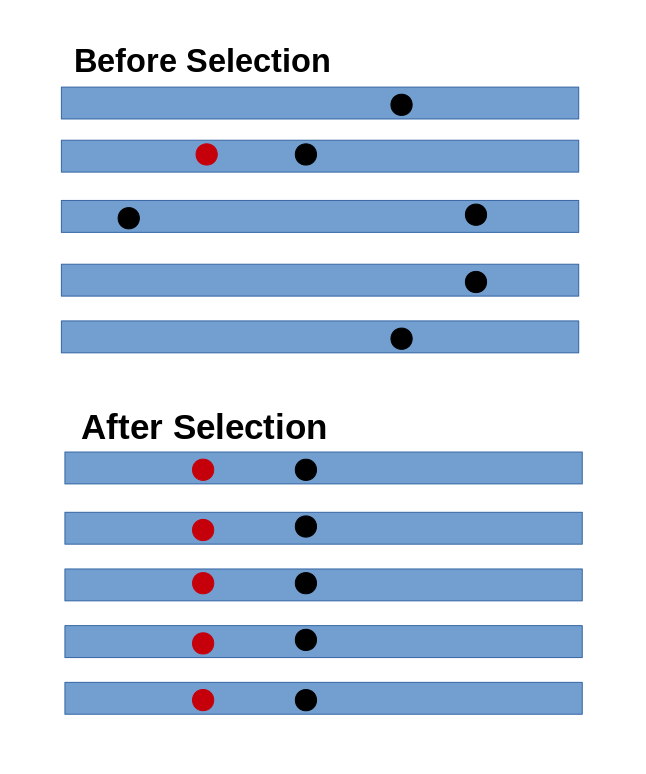
\includegraphics[width=0.5\linewidth]{images/sweep_diagram} 

}

\caption[Diagram of hard selection sweep.]{Representation of alleles before and after a hard
sweep. Each rectangle represents a haplotype within a population. A new
mutation is shown in red and neutral alleles are shown in black. After a
hard sweep the new mutation becomes fixed in the population, along with
the neutral allele that is linked to it.}\label{fig:sweepDiagram}
\end{figure}

A soft sweep occurs when an initially fitness-neutral allele evolving
under drift experiences a beneficial environmental change and increases
in frequency until fixation. The initial neutral nature of the allele
prior to becoming beneficial means there is a range of surrounding
haplotypes and there is not as much reduction in genetic diversity as
happens with a hard sweep
\citep{Hermisson2005, Schrider2015b, Hermisson2017}. The result of a
soft sweep is multiple haplotypes of intermediate frequency around the
selected site. If the selective environment for a population changes
frequently enough, soft sweeps could be the main method of adaptation
\citep{Schrider2015b}.

A partial or incomplete sweep occurs when part way through a sweep the
selective pressure is changed/removed resulting in an increase in
frequency for the allele that then returns to random genetic drift.

In order to determine if a selective event has occurred, one can attempt
to find what are termed ``signatures of selection''. Population
differentiation can sometimes be indicative of a selective event. If
extreme levels of differentiation are observed at a locus between
populations, this can be interpreted as evidence of positive selection.
Regions of the genome that have a reduction in variability in a
population can be the effect of a selective sweep. A third example of a
signature of selection is deviation in the frequency spectrum for
alleles beyond what would be considered possible under neutrality
\citep{Przeworski2002}. A key signature of positive selection is the
increase in proportion of high frequency variants
\citep{fay2000hitchhiking}.

Assuming a background of neutrality means that there needs to be a way
to identify variants under selection as opposed to population
demographic events, such as bottlenecks or expansions. In the case of
Polynesian settlement, there is evidence for a founder effect which
needs to be considered when interpreting selection results
\citep{Kayser2006a}. It is for this reason that the unique features of a
selective event need to be able to be identified from other possible
features such as population demography or admixture. Population events
and demography affect the entire genome, whereas selection acts on a
localised region \citep{Stajich2005}. To be able to recreate demography,
the choice in the \glspl{snp} used in the calculation of neutrality and
selection statistics is important as there is chance for a large
ascertainment bias if \glspl{snp} are only selected from a small number
of populations \citep{Wall2008}. The \glspl{snp} used also need to be
sampled away from genic areas.

\section{Methods for detecting selection}\label{selMethods}

Since 2005 there have been multiple reviews published (see
\citet{Nielsen2005}, \citet{sabeti2006positive}, \citet{Utsunomiya2015},
\citet{Vitti2013} and \citet{Haasl2016}) on methods of identifying
selection, as there has been a renewed interest to examine selection at
a genome wide scale due to increased availability of whole genome
genotype data. Methods that have been developed to detect signatures of
selection can be placed into two main categories, those that only work
on a single population and those that compare between populations. There
are also specific underlying genetic features that these methods can
use, such as allele frequency (frequency spectrum methods) or
differences in haplotype (linkage methods). Also, there are methods that
combine different approaches (composite methods). A summary of selection
methods is provided in Table \ref{tab:selectionMethods}.

The different methods for detecting selection work best over different
time periods. Recent soft sweeps are able to be detected well with
\gls{ld}-based methods, but frequency spectrum tests struggle
\citep{Hermisson2005}. The opposite applies in the case of hard sweeps
\citep{Hermisson2005}. In humans, the method that is able to detect the
most ancient selection, ranging to millions of years ago is the
K\textsubscript{a}/K\textsubscript{s} ratio, however if a strong
background of neutrality is present this can undermine the effectiveness
of the test. \Gls{td} is able to detect selection events as old as
250,000 years ago in regions of low diversity containing an excess of
rare alleles. \Gls{fwh} is able to detect events less than 80,000 years
ago based on derived alleles having arisen through mutation and then
risen to a high frequency via hitch-hiking. F\textsubscript{ST}, in the
range of less than 50,000 to 70,000 years ago, picks up geographic
separation of populations that have been subject to different physical
and cultural environments based on the changes in allele frequency in
one population versus another. Methods relying on long haplotypes such
as \gls{ihs} have the shortest range at less than 30,000 years ago for a
long haplotype that has not had time to break down through recombination
and contains a high frequency variant. Partial sweeps can also be
detected down to a \gls{maf} of approximately 10\%
\citep{sabeti2006positive}.

\begin{table}

\caption{\label{tab:unnamed-chunk-1} \label{tab:selectionMethods} Summary of Selection Methods}
\centering
\begin{tabular}[t]{l>{\raggedright\arraybackslash}p{10em}ll}
\toprule
Method & Detects selection within or between populations & Timeframe & Key reference\\
\midrule
\addlinespace[0.3em]
\multicolumn{4}{l}{\textbf{Macroevolutionary}}\\
\hspace{1em}Ka/Ks & Within and Between & Ancient selection & \citet{Hughes1988}\\
\hspace{1em}HKA & Within and Between &  & \citet{Hudson1987}\\
\addlinespace[0.3em]
\multicolumn{4}{l}{\textbf{Haplotypic}}\\
\hspace{1em}iHS & Within & < 30,000 years & \citet{voight2006map}\\
\hspace{1em}XPEHH & Between &  & \citet{tang2007new}\\
\hspace{1em}nSL & Within &  & \citet{Ferrer-Admetlla2014}\\
\addlinespace[0.3em]
\multicolumn{4}{l}{\textbf{Frequency spectrum}}\\
\hspace{1em}Tajima's \textit{D} & Within & < 250,000 years & \citet{Tajima1989}\\
\hspace{1em}Fay and Wu's \textit{H} & Within & < 80,000 years & \citet{fay2000hitchhiking}\\
\hspace{1em}Fu and Li's \textit{F} & Within &  & \citet{Fu1993}\\
\hspace{1em}Zeng's \textit{E} & Within &  & \citet{Zeng2006}\\
\hspace{1em}F\textsubscript{ST} & Between & < 50-70,000 years & \citet{Weir1984}\\
\hspace{1em}$\Delta$DAF & Between &  & \citet{Grossman2010}\\
\hspace{1em}SCCT & Within &  & \citet{Wang2014}\\
\addlinespace[0.3em]
\multicolumn{4}{l}{\textbf{Composite}}\\
\hspace{1em}CLR & Within &  & \citet{Kim2002}\\
\hspace{1em}XP-CLR & Between &  & \citet{Chen2010}\\
\hspace{1em}CMS & Within and Between &  & \citet{Grossman2010}\\
\hspace{1em}Meta-SS & Within and Between &  & \citet{Utsunomiya2015}\\
\hspace{1em}CSS & Within and Between &  & \citet{Randhawa2014}\\
\bottomrule
\end{tabular}
\end{table}

\subsection{Macroevolutionary methods}\label{macroevolutionary-methods}

\subsubsection{\texorpdfstring{K\textsubscript{a}/K\textsubscript{s}}{Ka/Ks}}\label{kaks}

The ratio of non-synonymous to synonymous mutations is called the
K\textsubscript{a}/K\textsubscript{s} ratio (or
d\textsubscript{N}/d\textsubscript{S} ratio as it is often referred to),
and is used to infer functional impact from selection, since synonymous
mutations are thought of as silent mutations with a neutral effect on
the protein \citep{Hughes1988}. K\textsubscript{a} is the number of
non-synonymous differences between sequences normalised by the total
number of non-synonymous sites in the sequence. K\textsubscript{s} is
likewise, but for synonymous differences normalised by the total number
of synonymous sites in the sequence. Comparing the baseline rate of
mutation (synonymous) to the non-synonymous rate gives an understanding
of the tolerance of amino acid alternatives in the protein, with an
excess of non-synonymous mutations indicating the novel protein
structures are being favoured and the protein is being positively
selected for. A K\textsubscript{a}/K\textsubscript{s} ratio greater than
1 is indicative of positive selection, while a value less than 1 is
indicative of negative selection against deleterious mutations and for
keeping the protein conserved.

\subsubsection{HKA}\label{hka}

The HKA test \citep{Hudson1987} compares between and within populations
the polymorphism and divergence of two or more loci, and uses this to
establish if a locus has been under selection, since variation within,
and diversity between, species under neutrality should be based only on
the mutation rate. The assumption that mutation rates at neutral loci
are constant over time is important, because if the rate changes, it
will affect the difference between the polymorphism and divergence. In
practice the HKA test is powered for recent selection events, however,
in practice it is difficult to find a putatively neutral locus
\citep{Zhai2009}.

\subsection{Haplotypic methods}\label{haplotypic-methods}

There are a few methods that are different derivations and applications
of looking at haplotype decay around a core \gls{snp}.
\citet{sabeti2006positive} put forward the concept of using \gls{ehh}.
The haplotypes that had unusually long haplotype homozygosity and a high
frequency in the population indicated that the polymorphism had risen in
prominence faster than it would be expected under the neutral model and
therefore under selection. The main concept is that a beneficial
mutation would not solely be selected for, with the surrounding region
initially ``hitch-hiking'' and therefore it would have a conserving
effect. As time and generations progressed, this haplotype would decay
due to recombination, and this haplotype decay can be used to assist in
the ageing of the selection event. In order to use haplotypic methods,
there is a requirement to establish the alleles that were inherited from
the maternal side and those that were inherited from the paternal side
constituting the two haplotypes (phasing).

\subsubsection{Integrated haplotype homozygosity
score}\label{integrated-haplotype-homozygosity-score}

The \gls{ihs} \citep{voight2006map, Szpiech2014} calculation starts with
\gls{ehh}, which is the probability that 2 chromosomes carrying a core
haplotype are homogenous to the distance \(x\). A value of 0 represents
no homozygosity, meaning all haplotypes are different, while a value of
1 is complete homozygosity meaning all haplotypes are the same. The
\gls{ehh} value versus distance is integrated to find the area under
\gls{ehh} curve until \gls{ehh} decays to 0.05. This \gls{ihh} is
calculated based on the ancestral or derived allele and annotated as
\gls{ihh}\textsubscript{A} or \gls{ihh}\textsubscript{D}. The
unstandardised \gls{ihs} is calculated in equation \eqref{eq:ihs}, which
is the \texttt{selscan} version \citep{Szpiech2014}. Standardisation of
\gls{ihs} is shown in equation \eqref{eq:stdihs}, where the expectations
and standard deviation of equation \eqref{eq:ihs} are estimated from the
empirical distribution of SNPs where the \gls{daf} (see section
\ref{dafsection}) p matches the frequency at the core \gls{snp}
\citep{voight2006map}. Large positive values indicate long haplotypes
carrying the derived allele, whereas negative values indicate haplotypes
carrying the ancestral allele. The calculation in \citet{voight2006map}
has \gls{ihh}\textsubscript{A} and \gls{ihh}\textsubscript{D} switched.
The \citet{Szpiech2014} \gls{ihs} calculation is used in this thesis
(equations \eqref{eq:ihs} and \eqref{eq:stdihs}). \Gls{ihs} identifies
variants under selection driven to intermediate frequencies.

\begin{equation} 
iHS_{unstd} = \ln{\frac{iHH_D}{iHH_A}}
\label{eq:ihs}
\end{equation}

\begin{equation} 
iHS_{std} = \ln{\frac{iHH_D}{iHH_A}} - \frac{E_p [\ln{\frac{iHH_D}{iHH_A}}] }{ SD_p [\ln{\frac{iHH_D}{iHH_A}}] }
\label{eq:stdihs}
\end{equation}

\subsubsection{Cross population extended haplotype
homozygosity}\label{cross-population-extended-haplotype-homozygosity}

\Gls{xpehh}, created by \citet{tang2007new}, is also known as Rsb.
\Gls{xpehh} was designed for use with \gls{snp} data rather than
sequence. \Gls{xpehh} lacks power to detect intermediate frequency
variants but is designed to detect variants that are near fixation or
completely fixed. The \gls{ehh} of \gls{snp} site (EHHS), integrates to
sum the area under the decay by distance in \gls{ehh} (iHH) which is
then used as a log ratio between populations at a single site (equation
\eqref{eq:xpehh}) and in a standardised form (equation \eqref{eq:xpehhstd}),
with 1 and 2 indicating the population. Recombination rate is mostly
conserved within populations, so provides an internal control in
\gls{xpehh} for effects of heterogeneous recombination rates. Extreme
values of \gls{xpehh} indicate a slower decay of \gls{ehh} in one
population compared to the other. \Gls{xpehh} relies on the breakdown of
\gls{ld} over time and has weak power to detect selective sweeps that
were historical and ended thousands of generations ago \citep{Chen2010}.
F\textsubscript{ST} is better than \gls{xpehh} for differential
selection between closely related populations because haplotype-based
signals are mostly shared between geographically similar populations
\citep{pickrell2009signals}.

\begin{equation} 
 XPEHH_{unstd} = \ln{\frac{iHH_1}{iHH_2}}
\label{eq:xpehh}
\end{equation}

\begin{equation} 
 XPEHH_{std} = \frac{\ln{\frac{iHH_1}{iHH_2}} - E [ \ln{\frac{iHH_1}{iHH_2}} ]}{ SD [ \ln{\frac{iHH_1}{iHH_2}} ]}
\label{eq:xpehhstd}
\end{equation}

\subsubsection{Number of segragating sites by
length}\label{number-of-segragating-sites-by-length}

\Glsdesc{nsl} is another single population haplotypic method that is
extremely similar to \gls{ihs}, however \gls{nsl} also measures the
length of a segment of haplotype homozygosity between a pair of
haplotypes in terms of number of mutations in the remaining haplotypes
in the data set in the same region \citep{Ferrer-Admetlla2014}.
Demographic events affect \gls{nsl} less than \gls{ihs}. Under
simulations for different demographic events, \gls{nsl} had a smaller
total difference in variation between the standard distribution of the
test statistic and the distribution of the modelled demographic event
\citep{Ferrer-Admetlla2014}.

\subsection{Frequency spectrum
methods}\label{frequency-spectrum-methods}

The frequency spectrum methods are based on finding deviations in the
frequency spectra of alleles that are outside of what would be expected
under neutrality. These can involve an increase in particular types of
frequencies such as low, intermediate, high variant frequencies, or a
difference in allele frequencies between populations.

\subsubsection{\texorpdfstring{Tajima's
\emph{D}}{Tajima's D}}\label{tajimas-d}

\gls{td} \citep{Tajima1989} counts the number of segregating sites of
individuals in a population and finds the ratio between polymorphisms
and pair-wise individual comparisons. \Gls{td} is a test of the neutral
hypothesis. The hypothesis is rejected when there is an excess of low
frequency variants. A negative \gls{td} is indicative of positive
selection or weak negative selection but a negative value can also be
attributed to population events such as population expansion. Positive
values of \gls{td} indicate an excess of intermediate frequency
variants. An excess of intermediate frequency variants could also be
attributed to balancing selection, population structure, or population
bottlenecks \citep{Kreitman2000, Nielsen2005, nielsen2007recent}. The
comparison of other polymorphisms, such as changes in \glspl{snp} versus
changes in \gls{indel} numbers can provide further evidence for either
selection or a population event, since population events should affect
both \glspl{snp} and \glspl{indel} in an equal fashion. The direction
(positive, zero, or negative) of \gls{td} values after a population
bottleneck depends on the strength and duration of the bottleneck and
can generate similar \gls{td} values, and can be positive, negative or
zero \citep{Fay1999}. After a population reduction or selective event,
it is expected the population will have excess rare alleles (recent, low
frequency) as the population recovers, therefore \gls{td} will be
negative \citep{Barton1998}. \Gls{td} is sensitive to sequencing errors
that are called as \glspl{snp} because they appear equivalent to low
frequency variants \citep{Achaz2008}.

\subsubsection{Fu and Li's F}\label{fu-and-lis-f}

\gls{flf} is the comparison of the number of derived singleton mutations
and the mean pair-wise difference between sequences \citep{Fu1993}. It
can be calculated both with or without an out-group
(\emph{F}\textsuperscript{*}), with Fu and Li's
\emph{F}\textsuperscript{*} having the greatest power of the Fu and Li
statistics \citep{Fu1993, Ramirez-Soriano2008}.

\subsubsection{\texorpdfstring{Fay and Wu's
\emph{H}}{Fay and Wu's H}}\label{fay-and-wus-h}

\gls{fwh} is sensitive to \glspl{snp} rising to moderate to high
frequency and uses an out-group (such as the ancestral reference
sequence) to determine the derived/ancestral state of the allele. A
positive value indicates a deficit in derived moderate to high frequency
\glspl{snp}. A negative value indicates an excess of derived moderate to
high frequency \glspl{snp}. \Gls{fwh} rejects neutrality when there is
an excess of high but not low frequency variants. An increase in the
proportion of high frequency variants compared to intermediate frequency
variants is a unique signature of positive selection
\citep{fay2000hitchhiking}. \Gls{fwh} can be used in regions of low
recombination to distinguish hitch-hiking from neutral or background
selection where it is expected there will be the same level of
intermediate to high frequency variants.

\subsubsection{Zeng's E}\label{zengs-e}

In contrast to \gls{fwh} and \gls{td}, which compare either high or low
frequency variants with intermediate frequency variants, \gls{ze}
compares the low and high frequency variants \citep{Zeng2006}. After a
selective sweep, the lower frequency variants are expected to `bounce
back' faster than the higher frequency variants. The \emph{E} test is
not sensitive to population subdivision. A negative value for \gls{ze}
is indicative of a selective sweep, but a rapid population expansion can
also produce a negative value.

\subsubsection{\texorpdfstring{F\textsubscript{ST}}{FST}}\label{fst}

F\textsubscript{ST} is a population differentiation metric that measures
the differences in heterogeneity of a sub-population compared to a
global population. Initially created by \citet{Wright1951}, as an
inbreeding coefficient for inbreeding as a whole in a population
(equation \eqref{eq:fst}), F\textsubscript{IT} is the inbreeding
coefficient for the individual in the total population and
F\textsubscript{IS} is the inbreeding coefficient for inbreeding of the
individual in the subpopulation. Both F\textsubscript{IT} and
F\textsubscript{IS} compare the observed heterozygosity of the
individual with the expected heterozygosity in either the total
population (F\textsubscript{IT}), or the subpopulation
(F\textsubscript{IS}). These fixation indices provide ways of
summarising population structure. Selection will act to drive an allele
to fixation, whereas immigration usually reduces the frequency. When the
selective advantage is strong, selection will be the dominant force on
the locus, however, when the selective advantage approaches zero, the
allele will begin to act neutrally and disappear with a probability of
one minus its frequency \citep{kimura_genetic_1968}. Cockerham
\citetext{\citeyear{Cockerham1969}; \citeyear{Cockerham1973}} equated
\(\theta\) (population genetic differentiation) with
F\textsubscript{ST}, extending F\textsubscript{ST} from calculating
population structure to population differentiation too. The fixation
indices were further developed by \citet{Weir1984} to add population
size weightings to the calculation. F\textsubscript{ST} values fall
between 0 and 1, each representing the fixation of an allele. Large
differences in F\textsubscript{ST} values are indicative of population
differentiation, suggesting directional selection at that locus, whereas
small differences in F\textsubscript{ST} indicate that the populations
are similar. F\textsubscript{ST} can have high variation in neighbouring
loci under neutrality \citep{Weir2005}. Unless populations are closely
related, such as northwest and southeast Europeans \citep{Price2008a},
the noise will drown out the signal, and identification of genome-wide
significance in F\textsubscript{ST} will be difficult. \citet{Weir2005}
suggested taking a sliding window approach to help improve the signal to
noise ratio.

\begin{equation} 
F_{ST} = \frac{F_{IT}{-}F_{IS}}{1{-}F_{IS}}
\label{eq:fst}
\end{equation}

F\textsubscript{ST} has been used in multiple studies as evidence for
natural selection
\citep{myles2007identification, pickrell2009signals, Akey2012}.
\citet{Akey2012} used F\textsubscript{ST} at individual loci and
compared this to the distributions for the genome, chromosome and gene
levels. The use of the empirical distribution to compare to
F\textsubscript{ST} for each \gls{snp} controlled for the effects of
demography. F\textsubscript{ST} as a method for detecting selection was
developed further into d\textsubscript{\emph{i}}, which is a function of
pair-wise F\textsubscript{ST} between population \emph{i} and the
remaining populations \citep{Akey2010}. Outside of the human context
F\textsubscript{ST} has been a very popular method of reporting both
population structure and evidence of selection
\citep{Akey2010, Hancock2011, Qanbari2011, Wei2015b}. The population
branching statistic is a F\textsubscript{ST} based statistic that
involves the use of an out-group to compare estimates in divergence time
between populations \citep{Yi2010b}.

\subsubsection{Selection by conditional coalescent
tree}\label{selection-by-conditional-coalescent-tree}

Selection by conditional coalescent tree (\citet{Wang2014}) detects
recent positive selection by searching for an imbalance of genetic
variants and conditions these on the allele frequencies of the candidate
loci. Selection by conditional coalescent tree pinpoints the causal
variant more accurately by using a method that is based on the
conditional coalescent tree method from \citet{Wiuf1999}, where
haplotypes are partitioned into two subgroups according to the allelic
state at a particular locus. It is assumed one subgroup carries the
derived allele at the locus and the other subgroup carries the ancestral
allele. The coalescence of a sample of haplotypes, conditioning on the
particular mutation, means each group should coalesce together
individually before the two subgroups coalesce. This is a similar idea
to that of \gls{ehh} used by \gls{ihs}, and the results of \gls{ihs} and
selection by conditional coalescent tree tend to be similar. The
selection statistic (S) is based on comparing the lineage lengths of the
two groups. Under neutrality S approaches \(\theta\), with significant
departures from \(\theta\) being considered evidence of positive
selection. When natural selection has a strong hitch-hiking effect on a
selectively favoured allele, selection by conditional coalescent tree
(and \gls{ihs}) is more powerful than \gls{td}, Fay and Wu's \emph{H},
and measuring change in derived allele frequency (see \ref{dafsection}).
In most cases the power of selection by conditional coalescent tree is
equivalent to \gls{ihs} except when selection is very strong, in which
case \gls{ihs} has more power \citep{Wang2014}. The power of selection
by conditional coalescent tree can be improved by increasing the sample
size. Selection by conditional coalescent tree performs moderately with
population demographic events (such as bottlenecks) and out performs
\gls{td} and \gls{ihs} in false discovery rate, although it does not
perform as well as \gls{fwh} \citep{Wang2014}.

\subsubsection{Change in derived allele frequency}\label{dafsection}

Similar to F\textsubscript{ST}, \gls{ddaf} looks at population
differentiation. The derived allele is determined through the use of an
ancestral out-group such as chimpanzees when used in human populations.
\Gls{daf} itself is calculated by determining the ancestral and derived
state for an allele and calculating the allele frequency with regard to
the derived state. \gls{ddaf} measures the absolute difference in the
derived allele frequency between two populations \citep{Grossman2010}
and has greater power to detect sweeps, both partial and complete, and
outperforms \gls{xpehh} for partial sweeps \citep{Colonna2014}.
\gls{ddaf} is part of the composite of multiple sites statistic
\citep{Grossman2010} but has also been used as a standalone metric in
humans \citep{Colonna2014, Gudbjartsson2015} and in other species such
as cattle \citep{Randhawa2014} to measure differentiation.

\subsection{Composite methods}\label{composite-methods}

Composite methods combine multiple methods with the goal of increasing
overall power and/or spatial resolution for detecting selection. The
combination of methods also gives greater resilience against demographic
events.

\subsubsection{Composite likelihood
ratio}\label{composite-likelihood-ratio}

The composite likelihood ratio (CLR), created by \citet{Kim2002}, is a
test for local hitch-hiking selection along a recombining chromosome. It
calculates a null distribution of variation from neutral coalescent
simulations involving recombination, and uses this to calculate the
probability of observing a threshold ratio of segregating variants. The
\citet{Nielsen2005a} version of composite likelihood ratio is similar to
Kim and Stephan's test but creates the null distribution from the data
itself, instead of using the neutral population model. A key
consideration for the use of composite likelihood ratio is that it is
very sensitive to \gls{snp} ascertainment bias \citep{Chen2010}.

\subsubsection{Cross population composite likelihoods
ratio}\label{cross-population-composite-likelihoods-ratio}

The cross-population composite likelihoods ratio (XP-CLR) is an
extension of the composite likelihood ratio test developed by
\citet{Nielsen2009} that scans for multi-locus allele frequency
differentiation between two populations and then tests if these
frequency differences are too recent to be consistent with neutrality
based on the \gls{ld} in the region \citep{Chen2010}. A down-weighting
of \glspl{snp} that are in perfect or high \gls{ld} is performed because
they essentially provide the same information. By doing this it is hoped
that false positives are reduced, since the correlation of marginal
likelihood terms in the composite likelihood function is often
overlooked and leads to false positives. Normalised cross-population
composite likelihoods ratio scores should be resistant to variation in
demographic events, however a conservative approach of using rank-order
of scores across the genome is usually taken. Unlike single population
composite likelihood ratio and similar to \gls{xpehh}, cross-population
composite likelihoods ratio is resistant to \gls{snp} ascertainment bias
because population differentiation is not affected by ascertainment
bias. There is also a strong correlation between genes identified with
cross-population composite likelihoods ratio and \gls{xpehh}.
cross-population composite likelihoods ratio is also considered an
extension of F\textsubscript{ST} and is beginning to be used as a
replacement for investigating selection in animal studies (e.g., Cattle
-- \citet{Lee2014}; Goats - \citet{Benjelloun2015})

\subsubsection{Composite of multiple
signals}\label{composite-of-multiple-signals}

Composite of multiple signals (CMS) is a combination metric composed of
\gls{ihs}, \gls{xpehh}, F\textsubscript{ST}, \gls{ddaf}, and
\(\Delta\)\gls{ihh}. \(\Delta\)\gls{ihh} is used to compare the actual
length of the haplotype. Composite of multiple signals was created to
take advantage of the combined power gained from using all metrics
together to be able to detect the source of the selective signal better
than any test individually could \citep{Grossman2010}. In composite of
multiple signals, it was found that \gls{xpehh} and F\textsubscript{ST}
contributed mostly to spatially locating the causal variant whereas
\gls{ihs}, \gls{ddaf}, and \(\Delta\)\gls{ihh} did poorly in spatially
locating the selective signal but performed well at identifying the
precise causal variant.

\subsubsection{Meta-analysis of multiple
tests}\label{meta-analysis-of-multiple-tests}

Meta-analysis of multiple tests (meta-SS)
\citep{Utsunomiya2013, Utsunomiya2015} is only able to combine selection
statistics that generate P-values. It uses an adapted version of a
weighted Stouffer method \citep{stouffer1949american, Zaykin2011} to
combine Z-transformed P-values. For each marker from each test \emph{i}
the respective P-value is transformed into a Z score by
Z\textsubscript{i} = - \(\phi\) -1(1 - \(\pi\)), where \(\phi\) is the
normal cumulative density function. Each test is weighted
(w\textsubscript{i}) to 1/n where n is the number of comparisons. The
combined statistic of \(k\) tests, for each \gls{snp} in each population
is defined in equation \eqref{eq:metass}.

\begin{equation} 
meta\-SS = \frac{\sum\limits_{i =1}^k {\omega_i Z_i}}{\sqrt{\sum\limits_{i =1}^k {\omega_i}^2}}
\label{eq:metass}
\end{equation}

\subsubsection{Composite of selection
signals}\label{composite-of-selection-signals}

Composite of selection signals (CSS) is similar to meta-analysis of
multiple tests, in that it is a method for combining the results from
multiple selection tests but is not limited to tests that produce
P-values \citep{Randhawa2014}. Composite of selection signals currently
uses F\textsubscript{ST}, \gls{xpehh}, and \gls{ddaf} or change in
selected allele frequency, and combines them by taking the test
statistic for each method across each \gls{snp}(1,\ldots{},n) then
obtaining the rank of each statistic across each \gls{snp}(1 \ldots{} n)
and converting these into fractional ranks so they lie between 0 and 1,
that is, 1/(n+1) to n/(n+1). By doing this the magnitudes of the
original statistics are not used, thus increasing the robustness. The
fractional ranks are converted to Z-statistics and the average z-values
are calculated at each \gls{snp} position. P-values are obtained from
the distribution of the means with the -log10(p) being the composite of
selection signals value. The composite of selection signals is plotted
against genomic position with an excess in the number of values at a
position showing a common signal between the multiple test statistics.

\subsection{Power}\label{power}

Power to detect selected sites can be very limited if the site is not an
outlier from empirical methods, such as simulations or using
permutations of the data, as they would not `stand out'
\citep{Teshima2006}. A key consideration when selecting a particular
method for detecting selection is the limitations the method has on
power to detect a selective event, such as starting and final allele
frequency of the variant after a sweep. \Gls{td} is powered for low and
intermediate frequency variants \citep{Simonsen1995} whereas \gls{fwh}
is powered for intermediate and high frequency variants. Some methods
such as \gls{ihs}, are good for detection of middle frequency variants.
\Gls{xpehh}, on the other hand is powered at the fixation ends of the
spectrum. \Gls{xpehh}, because it is correlated with \gls{ld}, lacks
power to detect ancient selective events \citep{Chen2010}. Sample size
is another factor to consider. \Gls{ihs} has modest reduction of power
when reducing samples until approximately 40 samples of single
chromosomes. \Gls{xpehh} can maintain power down to about 20 samples of
single chromosomes, so long as the reference population is a fixed size.
The grouping of similar genetic populations may be an option to increase
power with low sample sizes \citep{pickrell2009signals}). For
F\textsubscript{ST}, power to detect selection should be sufficient if
sample size is \textgreater{} 1/F\textsubscript{ST}
\citep{Bhatia2011, Bhatia2013a}

Power of a statistic also needs to be considered for the type of
selective sweep that may have occurred, such is the case with \gls{nsl},
which has similar power to detect selection to \gls{ihs}, but performs
better for larger starting allele frequencies. It also outperforms
\gls{ihs} in power in both hard and soft sweep scenarios
\citep{Ferrer-Admetlla2014}. When it comes to picking up demographic
events, haplotype tests are useful at detecting recent and more moderate
bottlenecks, frequency spectrum tests (such as \gls{fwh}/ \gls{td}) have
the best power for detecting moderately ancestral severe bottlenecks
\citep{Depaulis2003}, whereas \gls{ze} and \gls{flf} have the most power
during population expansion \citep{Zeng2006, Ramirez-Soriano2008}.
Assessment of power to detect selection has previously been done through
simulation or the use of well established loci as positive controls
\citep{voight2006map, Zhai2009, Cadzow2016}. When simulating, it
important to generate scenarios that include different demographic
events as well as selection events. Simulated models are generally done
in one of three ways, as a coalescent model, or a forward-in-time model,
or by resampling \citep{Yuan2012}. The coalescent model (and most
commonly used) works backwards-in-time to find the most recent common
ancestor, and then permutes through models to arrive at the current
state \citep{kingman_genealogy_1982, Yuan2012}. The forward-in-time
simulations will take a starting ancestral population and then apply a
population model, iterating through subsequent generations
\citep{peng_forward-time_2010, Yuan2012}. Another approach can be to
take the observed data and shuffle and resample it to generate empirical
distributions. From each of these methods false positive and false
negative rates can be calculated.

\subsection{Challenges}\label{challenges}

When scanning genome-wide in a population (such as in a \gls{gwas}, or
genome-wide selection scan), the variability in the genome also has
population demographic events that have acted upon it, such as
population bottlenecks, migration, or growth. Mutation and recombination
are also acting on the genome. Methods based on comparing non-synonymous
to synonymous variants are relatively unaffected, but methods based on
allele frequency are susceptible to detecting population demographic
events, along with mutation and recombination rate changes
\citep{Nielsen2009}. A meta population is a population which can be
subdivided into many different sub-populations among which there is some
pattern of migration, extinction, and recolonization
\citep{Wakeley2001}. Bottlenecks with a meta-population model can lead
to a high frequency of derived alleles, greater than would be expected
to arise through a neutral model \citep{Jensen2005} and as previously
mentioned by \citet{fay2000hitchhiking} about high frequency derived
alleles being a unique signature of selection, it not actually unique
\citep{Przeworski2002}.

\Gls{snp} ascertainment bias is caused by the non-random sampling of
SNPs on array chips. This is a problem that affects the selection
detection methods to different extents, with frequency spectrum methods
being the most susceptible. \Gls{td} is biased upwards due to the
\gls{snp} discovery process having ascertainment biases, which leads to
an excess of intermediate frequency alleles in the sample
\citep{Kelley2006}. Tests that rely on long haplotypes are less
susceptible to ascertainment bias \citep{sabeti2006positive} but because
long haplotypes can be quickly broken down through recombination, they
are only useful for short time periods. \Gls{snp} ascertainment bias can
be overcome with the use of whole genome sequencing
\citep{Albrechtsen2010}.

Many of these statistics were developed to investigate selection at a
particular locus, at a time when applying the statistics across a genome
was not possible. Up until recently, genome scans have been performed
using \gls{snp} genotypes identified through a \gls{snp} discovery
process, which means they are not random samples -- which would include
non \gls{snp} genotypes (such as \glspl{indel}) and create an
ascertainment bias \citep{Nielsen2005a}

Identification of exactly what is deemed as being ``significantly
selected''" has issues. The current practice is to take outlier loci,
usually from an empirical distribution of the selection statistic and
report these as significant. This is not necessarily indicative of
selection, as cut off levels are created subjectively rather than
derived from the model \citep{Qanbari2012a}. Using an empirical approach
will result in many false positives, however this is considered an
acceptable approach for selecting candidate genes so long as it is
realised that the false positive rate is high \citep{Kelley2006}.

In order to use haplotypic methods, (re)construction of haplotypes is
required. Currently this involves the need for the phasing of haplotypes
from genomic data. Phasing is the process of determining which alleles
are found together on the same physical chromosomes. There are a number
of ways that this can be done, such as through a pedigree, through the
use of large population data, or using the reads from next generation
sequencing. Phasing through pedigree information is utilised in most
agricultural species, whereas for human populations the population
genotypes are largely from unrelated individuals. Phasing of unrelated
individuals currently relies on probabilistic methods
\citep{Browning2009, Delaneau2012, Delaneau2013} in order to make the
best guess at each individual haplotype. Newer methods have been
developed to use the reads from next generation sequencing and are able
to trace a haplotype across multiple overlapping reads and be used to
complement other probabilistic phasing methods, however these
read-backed methods are dependent on the depth of coverage and read
quality \citep{Delaneau2014}.

\section{Improving GWAS}\label{improving-gwas}

\Gls{gwas} is a method to scan genomes, usually \gls{snp} genotype data,
for association with a phenotype. Association is usually tested between
a trait and a single \gls{snp} using either linear regression
(continuous variable) or logistic regression (binomial variable), with
confounders included where possible as covariates to the models. These
association tests are repeated for each \gls{snp} across the genome (for
a comprehensive explanation of \gls{gwas} methods see
\citet{bush_chapter_2012}). Commonly an additive model is used for the
\gls{snp}. The strength of \gls{gwas} is that prior knowledge of loci is
not required and can be used as a tool for hypothesis generation.
\Gls{gwas}, because of the large number of association tests, require
large cohorts of samples to achieve sufficient power for statistical
significance. As the effect size for a variant decreases, larger sample
sizes are also needed, as power is proportional to the square of the
effect size \citep{Hemani2013, Korte2013}. Limitations in recruiting
sufficient numbers of participants for \gls{gwas} therefore requires new
ways of increasing power to detect smaller effects without needing to
increase sample size, as outlined in this section. The goal of being
able to prioritise \gls{gwas} results by using additional information,
such as incorporating \gls{ld} or selection statistics by using a
weighting system to increase the power of a \gls{gwas}, has been
suggested \citep{Roeder2006, Ayodo2007}. When \gls{ld} between observed
\glspl{snp} and causal variants is high, such as in the case of
selection, greater power in \gls{gwas} can be achieved by focusing on
searching for non-additive variance \citep{Hemani2013}.

The basis of \gls{gwas} studies is to identify \glspl{snp} that are
associated with differences in the mean of a trait. These studies do not
necessarily identify the causal \gls{snp} but instead identify a marker
for the causal variant, usually in \gls{ld}. \citet{Fisher1919} showed
that total genetic variance could be split into components of additive,
dominance and epistatic effects. The additive component has been shown
to contribute the most to the overall genetic variance, with epistatic
variance contributing little in an outbred population \citep{Hill2008}.
Complex traits gain their complexity from being the sum of interactions
from many small effect loci, or the product of non-additive interactions
between loci and the environment, making it challenging to find the
exact contribution of a locus to a trait \citep{Fu2013a}. These small,
true effect loci can end up non-significant due to the noise in the data
but might be retrieved using methods that find non-additive effects.

Explained heritability is defined as the proportion of heritability (or
phenotypic variance) explained by a collection of genetic variants, with
the ``missing'' portion referring to the unaccounted genetic variance
that has been estimated through family studies. When the ratio of
explained heritability to total heritability is \textless{} 1, the
unexplained component is defined as missing heritability
\citep{Zuk2012}. The use of methods that capture additional loci with
non-additive effects should be able to explain more of missing
heritability.

\subsection{Selection and GWAS}\label{selection-and-gwas}

The significance of \gls{gwas} results is greatly increased when
selection statistics and association studies are combined, this has been
applied in a \gls{gwas} for malarial resistance variants
\citep{Ayodo2007}. A smaller sample size can be used if there is
evidence of positive selection because the beneficial allele will rise
in prevalence and be in high \gls{ld} with other variants (due to
genetic hitch-hiking) which can act as proxy markers
\citep{Karlsson2014}. The converse would apply for negative selection.
Complex disease traits compared to Mendelian disease associated traits
have a bias towards larger mouse-human
K\textsubscript{a}/K\textsubscript{s} ratios, by comparing the
K\textsubscript{a}/K\textsubscript{s} ratios for ortholog genes between
mouse and human, which suggests that evidence of positive selection
could be utilised in identifying variation associated with complex
disease \citep{Thomas2004}.

\subsection{Pathway analysis}\label{pathway-analysis}

A biological pathway is a dependency graph detailing the genes or
proteins involved in a series of biochemical reactions, such as a
metabolic pathway like the Krebs cycle. There are curated databases of
many of the biological pathways used by living organisms, such as
\gls{kegg} \citep{Kanehisa2017} or Reactome \citep{Fabregat2018}.
Pathways have been hypothesised to be involved in the genic adaptation
of populations since altering a gene in a biochemical pathway is likely
to alter different genes in the same pathway \citep{Bigham2010}. The use
of pathway analysis rather than focusing on individual \glspl{snp} is
another way to increase the power of a \gls{gwas} \citep{Jia2011}. This
increase in power is largely obtained through a reduction in
dimensionality in ways that attempt to remove noise from the underlying
biological signal. There are however limitations to the effectiveness of
using such an approach, such as the selection of pathway database,
density of \glspl{snp} per gene, or gene length and boundaries. The
pathway database is important because pathways can differ based on
curator, age of the database - with older databases not incorporating
current knowledge, or differing focuses. \Glspl{snp} per gene, and gene
length or boundaries all affect the pathway analysis as smaller genes or
\gls{snp} density reduces the observations for the gene compared to
large genes or genes with high \gls{snp} density. Pathways that involve
many large genes also have a higher chance of a \gls{snp} having an
extreme statistic value under a null model, because overall, they are
more likely to have more \glspl{snp} than pathways containing small
length genes.

\section{Applications}\label{applications}

\subsection{Genome-wide selection}\label{genome-wide-selection}

Genome-wide selection in humans has been investigated by
\citet{sabeti2006positive}, \citet{voight2006map}, \citet{Hancock2008},
\citet{pickrell2009signals}, the 1000 Genomes Project Consortium
\citep{1KGP2010, 1KGP2012, 1KGP2015snp}, \citet{Grossman2010},
\citet{Colonna2014}, and \citet{Mallick2016}. The population datasets
used involved the HapMap Project \citep{Hapmap2005}, the Human Genome
Diversity Project \citep{Cann2002, Rosenburg2002} and the 1000 Genomes
Project (populations are defined in section \ref{datasets};
\citet{1KGP2010}). The 1000 Genomes Project Consortium
\citep{1KGP2010, 1KGP2012, 1KGP2015snp} reported genome wide
diversification between main population groups based on
F\textsubscript{ST} and \gls{ddaf}. Genome wide mean F\textsubscript{ST}
was found to only be a maximum of 8\%, indicating overall little genetic
differentiation between populations, however several thousand SNPs had
large F\textsubscript{ST} indicating local population adaptation
\citep{1KGP2010}. The analysis also found 139 non-synonymous SNPs with
large frequency differences between populations. Investigation of the
\gls{1kgp} data set was also performed by \citet{Colonna2014}. Using
\gls{ddaf}, it was found that sites of high population differentiation
(\gls{ddaf} \textgreater{} 0.7 between and \textgreater{} 0.25 within
continents) clustered together, the same was found for sites of low
differentiation. Genes containing highly differentiated sites were
likely to also have additional evidence of positive selection in a
third. There was also a strong association of highly differentiated
sites with genes and gene regulatory elements.

Metabolic syndrome and gout have associations and interactions with
genes in metabolic pathways and the immune system \citep{Osborn2012}.
The categories of genes that have displayed evidence of selection from
the previously mentioned genome-wide selection scans include: metabolism
of sugars \citep{voight2006map, tang2007new}, drug metabolism
\citep{tang2007new}, immune system \citep{tang2007new, Grossman2010},
and climate adaptation \citep{Hancock2008}. Genes that play a role in
adaptation to climate extremes are likely to play a role in metabolic
disorders that make up metabolic syndrome \citep{Hancock2008}. In
contrast, variation in metabolic related genes can lead to elite
phenotypes in athletes, showing that metabolic genes also impact on
fitness \citep{Ahmetov2009a}.

\subsubsection{Selection in Polynesia}\label{selection-in-polynesia}

The inclusion of Oceanic populations in multi-population studies has had
a focus on genetic structure, measured via F\textsubscript{ST} for
differentiation to investigate population ancestry, rather than
selection \citep{Friedlaender2008, Tennessen2011}. The migratory history
of Polynesian populations suggests that the points of differentiation
are likely the events possibly occurring since the out of Africa
dispersal \textasciitilde{}60,000 years ago \citep{Soares2012} with
settlement of Near Oceania \textasciitilde{}40,000 years ago, and Remote
Oceania \textasciitilde{}3,100 years ago \citep{Matisoo-Smith2004} and
the Polynesian Triangle (bounded by New Zealand, Easter Island, and
Hawaii) \textasciitilde{}1,000-1,200 years ago \citep{Wilmshurst2011}.
The time frame for these events means that nearly all the previously
mentioned methods would still be within their powered time frames to
detect selective events. The haplotypic methods would possibly not be
able to detect selective events as old as the Africa dispersal and may
be at the fringe of the time period for the Near Oceania settlement.

Large population comparison studies have used Oceanic populations, but
analyses were limited to Melanesian and Papuan populations because the
cohort used was the Human Genome Diversity Project \citep{Cann2002}
which did not include Polynesian populations. The Melanesian and Papuan
populations are often used to infer the genetics of Polynesian
populations. This extrapolation does not take into account the current
ancestry predictions of Polynesians populations being more closely
related to Asian/Taiwanese Aboriginal populations than Melanesian
groups, or the presence of European admixture \citep{Friedlaender2008}.
Genomic DNA and mitochondrial DNA suggest Polynesians have East Asian
ancestry, with substantial male Melanesian admixture
\citep{Kayser2008a}. There has been limited analysis of selection in
Polynesian populations beyond \citet{Kimura2008}, where 24 Tongan
samples in conjunction with other populations were analysed using both
F\textsubscript{ST} and a modified \gls{ehh} test. Genomic regions with
evidence of having been selected in the Tongan samples were potential
candidates for increased fat, muscle and bone masses \citep{Kimura2008}.

A few candidate-genes for selection which also have been associated with
obesity and \gls{t2d} in Polynesian populations have been investigated,
such as the \emph{PPARGC1A} \citep{Myles2011} and \emph{CREBRF}
\citep{Minster2016} genes. The ``Thrifty-gene hypothesis''
\citep{Neel1962} has been the reasoning behind why these loci may have
undergone selection. The hypothesis was originally conceived to attempt
to explain the difference in prevalence of \gls{t2d}, that is, given
that there should be a strong selective pressure against it, there must
be some genetic advantage. This hypothesis has been challenged in the
Polynesian context as fitting a particular narrative
\citep{Gosling2014, Gosling2015, Cadzow2016} with an alternative
hypothesis being a link between the metabolic diseases and the innate
immune system that is under selective pressure via an infectious agent,
such as malaria, leading to disease susceptibility in these populations
\citep{Gosling2015}.

\subsection{Selection of metabolic syndrome and urate}\label{goutMetSyn}

The genetic influence of urate and gout is found in the under-excretion
of serum urate. There are 28 loci that have been identified as having a
role in hyperuricaemia and gout, of which, two (\emph{ABCG2} and
\emph{SLC2A9}) are responsible 3.4\% of the variability of urate
\citep{Kottgen2013}. \emph{SLC2A9} encodes a urate transporter expressed
on both the apical and baso-lateral membranes in the proximal tubule of
the kidney and reabsorbs urate \citep{Mandal2015}. \emph{ABCG2} encodes
an ATP powered urate transporter and is responsible for urate excretion
mostly in the gut \citep{Maliepaard2001, Mandal2015}. Twenty-six other
loci associated with serum urate explain a further 3.6\% of the variance
\citep{Kottgen2013}. The heritability of serum uric acid ranges from 40
- 70\% \citep{Yang2005, Nath2007}. This difference in explained
variability and total heritability leaves a large component yet to be
explained. This missing heritability could be reduced through
identifying additional variance attributed to non-additive effects.

There have been multiple genetic loci associated with \gls{t2d}
\citep{Billings2010} and \gls{bmi} \citep{Locke2015}, however,
\citet{Chen2010} found no evidence for enrichment in selection for
\gls{bmi}, but found significant enrichment for \gls{t2d}. The genes
associated with \gls{t2d} have been found to be differentiated by
population, however the individual \glspl{snp} are often not
\citep{pickrell2009signals}. \citet{Koh2014} identified six \glspl{snp}
in or near nine genes that had been reported as \gls{t2d} associated and
overlapped with evidence of positive selection in East Asian
populations. Common variants that have been found in European
populations associating with obesity do not replicate in the Samoan
population, although this is likely due to power \citep{Karns2012}. The
non-replication of European variants in Polynesians and the high
prevalence of obesity in Polynesian populations suggest there is likely
to be some population specific variants that are yet to be identified,
similar to the Polynesian specific variant in \emph{CREBRF}
(rs373863828), associated with obesity and protection for \gls{t2d},
identified in the Samoan population \citep{Minster2016}. Rare variants
tend to be recent and therefore geographically restricted
\citep{1KGP2012}.

The benefits of urate are in line with the categories found to be
enriched by selection in genome wide scans. Urate is an anti-oxidant in
the blood, acting to protect not just erythrocytes but also T and B
lymphocytes and macrophages \citep{Ames1981}. Urate has also been
hypothesised to have had a survival advantage during the Miocene period,
when a series of mutations in urate oxidase occurred, leading to
elevated urate. Hyperuricaemia enables blood pressure to be maintained
under low salt dietary conditions \citep{Watanabe2002}. Serum urate is
also a potent anti-oxidant which accounts for \textgreater{}50\% of the
anti-oxidant activity of the blood \citep{Glantzounis2005, Parmar2009}.
Later in life elevated serum urate is associated with increased
cognitive function \citep{Euser2009}. Urate crystals activate the NLRP3
inflammasome which plays an important role in systemic infection and
sepsis \citep{Opitz2009}. The role of urate in these situations shows
that while hyperuricaemia is now considered as contributing to disease
(such as gout), in the past it may have influenced longevity and
survival, therefore increasing reproductive success and being a
phenotype that has undergone selection.

An elevated prevalence of metabolic syndrome co-morbidities and
hyperuricaemia against a unique genetic background of Polynesian
populations provides an important opportunity to study the role and
effects that selection might have played on these metabolic conditions.

\section{Research purpose and aims}\label{research-purpose-and-aims}

This thesis seeks to understand selection in the context of Polynesian
populations, and the effect it may have played in the metabolic disease
burden that is present in these populations. There are three research
chapters, each with their own aims. In Chapter \ref{selectionResults}:
``Positive Selection in Polynesian Populations'', the aims were to
discover and characterise regions that have undergone selection in
Polynesian populations. In Chapter \ref{clustering}: ``Clustering of
Selection Statistics'', the aims were to investigate potential shared
ancestry regions that are relevant to urate and metabolic disease. And
in Chapter \ref{selGwas}: ``Selection and Association Studies'', the
aims were to investigate the use of gout definition in genetic
association studies, and the use of selection statistics in conjunction
with \gls{gwas} results.

It is hoped that the investigation of genetic selection in Polynesian
populations will further understanding of the cause of health
disparities due to metabolic disease in these populations.

\chapter{Methods and data}\label{methods-and-data}

This chapter describes the methods and datasets used in this thesis.
Section \ref{methods} covers the methods used for the preparation of the
datasets, such as haplotype phasing, \gls{pca}, and file format
conversions, as well as the methods used for the analysis of the
datasets, such as the calculation of selection statistics. Section
\ref{datasets} contains a description of the two main data sources that
were used and how they were transformed for the analysis.

\section{Methods}\label{methods}

All genomic resources and co-ordinates reported in this project use the
human genome reference build GRCh37, unless otherwise specified.

\subsection{Phasing}\label{phase}

Haplotype phasing is a method of establishing the parental origin of
haplotypes. It looks for the co-location of alleles to form haplotypes.
In diploids such as humans, there is a maternal and a paternal haplotype
at any given position in the genome. Selection statistics such as
\gls{ihs} require phased data in order to calculate the degradation of
haplotypes by recombination. Phasing can be performed through the use of
trios (parents and offspring), or it can be done through probabilistic
phasing using large population haplotype reference panels (such as
created from the \gls{1kgp}, see section \ref{kgpdesc} and Table
\ref{tab:refDatasets}) and probabilistically determining the most likely
haplotype(s) for an individual given a set of markers.

Phasing was performed using SHAPEIT2 v2.r837 \citep{Delaneau2013} using
the \gls{1kgp} reference haplotype panel (Table \ref{tab:refDatasets}).
There were two steps involved for phasing of genotypes. The first was to
check the markers in each data set were matched with the markers in the
reference haplotypes. Markers were marked for exclusion by this step for
reasons such as the marker not being in the reference panel, or if the
marker had different allele types to that in the reference panel. An
example of this step is provided in the following code.

\begin{Shaded}
\begin{Highlighting}[]
\CommentTok{# Check alignment of markers against reference haplotypes}
\CommentTok{# ? = chromosome}
\ExtensionTok{shapeit2}\NormalTok{ \textbackslash{}}
\NormalTok{-check \textbackslash{}}
\NormalTok{-M genetic_map_chr?_combined_b37.txt \textbackslash{}}
\NormalTok{--input-vcf coreExome_norm.chr?.vcf.gz \textbackslash{}}
\NormalTok{--input-ref 1000GP_Phase3_chr?.hap \textbackslash{}}
\NormalTok{  1000GP_Phase3_chr?.legend \textbackslash{}}
\NormalTok{  1000GP_Phase3.sample \textbackslash{}}
\NormalTok{  --output-log coreExome_norm.chr?.checked \textbackslash{}}
\NormalTok{  -T 12}
\end{Highlighting}
\end{Shaded}

The second step was the phasing of genotypes into their haplotypes by
using the \gls{1kgp} phased haplotype reference and a genetic map that
was provided as part of the reference files. Markers that were marked
for exclusion from the previous step were excluded. The most likely pair
of haplotypes were outputted. The haplotypes were then converted from
the haps format\footnote{\url{https://mathgen.stats.ox.ac.uk/genetics_software/shapeit/shapeit.html\#formats}}
into a phased \gls{vcf}\footnote{\url{https://samtools.github.io/hts-specs/VCFv4.2.pdf}}.
These two steps are shown in the following code.

\begin{Shaded}
\begin{Highlighting}[]
\CommentTok{# Run phasing against reference haplotypes}
\CommentTok{# Exclude misaligned markers}
\CommentTok{# Use 8 threads}
\CommentTok{# ? = chromosome}
\ExtensionTok{shapeit2}\NormalTok{ \textbackslash{}}
\NormalTok{-M genetic_map_chr?_combined_b37.txt \textbackslash{}}
\NormalTok{--input-vcf coreExome_norm.chr?.vcf.gz \textbackslash{}}
\NormalTok{--input-ref 1000GP_Phase3_chr?.hap \textbackslash{}}
\NormalTok{  1000GP_Phase3_chr?.legend \textbackslash{}}
\NormalTok{  1000GP_Phase3.sample \textbackslash{}}
\NormalTok{--output-max coreExome_norm.chr?.phased \textbackslash{}}
\NormalTok{--exclude-snp coreExome_norm.chr?.checked.snp.strand.exclude \textbackslash{}}
\NormalTok{-T 8}

\CommentTok{# Convert haps to vcf}
\ExtensionTok{shapeit2}\NormalTok{ \textbackslash{}}
\NormalTok{-convert \textbackslash{}}
\NormalTok{--input-haps coreExome_norm.chr?.phased \textbackslash{}}
\NormalTok{--output-vcf coreExome_norm.chr?.phased.vcf }
\end{Highlighting}
\end{Shaded}

\subsection{Selection Statistics}\label{selection-statistics}

\subsubsection{PopGenome}\label{popgenomeMethods}

The PopGenome package (v2.2.3, \citet{Pfeifer2014}) for R was used for
the calculation of \gls{td}, \gls{fwh}, \gls{flf}, and \gls{ze}.
Popgenome calculates the D* and F* version from \citet{Fu1993} which do
not require an outgroup that should be a closely related population or
species. The selection and neutrality statistics were calculated using a
sliding window approach with a window size of 100 kb and a slide of 10
kb. Windows that had fewer than four segregating sites were filtered
out, and window co-ordinates were altered to be +/- 5 kb from the centre
of the window. The empirical distribution for each statistic, for each
population, was used to create a significance threshold. The lower
threshold was \(min\)(1\textsuperscript{st} percentile, 0). The upper
significance threshold was \(max\)(99\textsuperscript{th} percentile,
0). The greater or less than zero condition was to enable the
interpretation of the selection and neutrality statistic results, as
zero is the point at which these statistics indicate an excess or
deficit of a particular allele frequency category. F\textsubscript{ST}
was also calculated in the same sliding window setup, and pair-wise
between the Polynesian populations and the other populations. Negative
F\textsubscript{ST} values were set to 0 because F\textsubscript{ST} is
biologically bounded to {[}0,1{]}. Negative values occur when the
variation within a population is larger than between populations.

The ancestral allele was used as annotated in the 1000 Genomes Phase 3
\gls{vcf} file where possible, for use as the out-group population. A
new sample identified as `Ancestor' was included in the phased
\gls{vcf}, and for each marker the genotype for this sample was set as
the homozygote for either the reference or alternate allele, dependent
on the ancestral allele matching, otherwise the Ancestor genotype was
set to missing. When the phased \gls{vcf} files were loaded into
PopGenome, populations were identified using panel files which were
white-space delimited files with sample id, population, and super
population as the columns. The out-group population for \gls{fwh} was
set to be that of the Ancestor sample so that the ancestral allele would
be used in the calculation.

\subsubsection{SelectionTools}\label{selectionTools}

SelectionTools v1.1 \citep{Cadzow2014} was used to generate the
haplotypic selection statistics of \gls{ihs}, \gls{nsl}, and
\gls{xpehh}. The combined population phased \gls{vcf} file was split
into individual populations. Within each population, markers were
filtered for a \gls{maf} of \textgreater{} 0.01 and a \gls{hwe} exact
test of P \textgreater{} 10\textsuperscript{-6} \citep{Wigginton2005}.
Markers were converted into ``ancestral'' or ``derived'' by comparing
alleles to the \textit{homo sapiens} ancestral fasta (see Table
\ref{tab:refDatasets}) with alleles that matched the ancestor set to 0,
and non-missing, non-matching alleles set to 1.

\gls{ihs}, \gls{nsl}, and \gls{xpehh} normalisation with frequency bins
of 0.05 was done using \emph{norm} as part of selscan v1.1.0b
\citep{Szpiech2014}. Markers with an \textbar{}\gls{ihs}\textbar{},
\textbar{}\gls{nsl}\textbar{} or \textbar{}\gls{xpehh}\textbar{} value
\textgreater{} 2.6 met the threshold for significance, which was
equivalent to approximately 1\% of the most extreme values.

Significant markers were also clustered into genomic regions using the
DBSCAN package v1.1.1 \citep{dbscanref} in R, where nearby \glspl{snp}
were assigned the same group identifier. The search radius used was 200
kb and the minimum number of points for a cluster was one. Cluster
regions were created by taking both the minimum and maximum position for
each group identifier, population, and chromosome.

\subsection{Disease associated gene lists}\label{diseaselist}

In order to create lists of genes that were associated with urate, gout,
obesity, \gls{t2d}, metabolic syndrome, and kidney disease, disease
trait entries were downloaded from the \gls{gwas} catalog\footnote{gwas\_catalog\_v1.0.1-associations\_e89\_r2017-06-19.tsv
  \url{https://www.ebi.ac.uk/gwas/} accessed 19 June 2017}
\citep{MacArthur2017}. The file was a rectangular format, with rows for
each study result, and columns such as reference paper, disease trait,
association statistics, and mapped genes. Entries were then filtered for
P \textless{} 5x10\textsuperscript{-8}. From the filtered results, the
kidney disease gene list was created by filtering the ``disease trait''
column to select rows with the keywords ``kidney'' or ``renal''. Entries
were then removed that had the keywords ``transplant'', ``carcinoma'',
``Type'', ``stones'', ``gout'', ``related'', or ``Diabetic kidney
disease''. For the gout, urate, obesity, \gls{t2d}, and metabolic
syndrome gene lists the following keywords were used on the ``disease
trait'' column to select rows of the P-value filtered data: ``metabolic
syndrome'', ``obesity'', ``diabetes'', ``urate'', ``gout'', ``body
mass'', and ``lipid traits''. This subset was then filtered to remove
rows containing these keywords in the ``disease trait'' column:
``child'', ``erectile'', ``lean'', ``autoantibodies'', ``gestational'',
``cancer'', ``psychopharmacol'', ``metaformin'', ``metformin'',
``obstructive'', ``interaction'', ``asthmatics'', ``omega'', ``pain'',
``cataracts'', ``time'', ``bilirubin'', ``chain'', ``thyroid'', ``zhi'',
``Type 1'', or ``cystic''. From this filtered data, keywords were used
to select rows relating to each trait of interest from the ``disease
trait'' column. The keywords ``urate'' and ``gout'' were used for gout
and urate, ``obesity'' and ``body mass'' used for obesity, ``diabetes''
used for \gls{t2d}, and ``syndrome'' used for metabolic syndrome. The
keywords ``kidney'' and ``renal'' were used for kidney disease, with
entries removed that had keywords of ``transplant'',
``carcinoma'',``type'', ``stones'',``gout'', ``related'', and ``Diabetic
kidney disease''.

Additional gene lists were created for malaria, auto-immune and
auto-inflammatory diseases, and neurological diseases. The keyword
``malaria'' was used to filter the disease trait column to create the
malaria gene list. The auto-immune and auto-inflammatory gene list was
based on diseases that were listed in Table 2 of \citet{Zhang2013a}. The
following keywords were filtered for in the disease trait column:
``Crohn's disease'', `Celiac disease', ``Ulcerative colitis'',
``Inflammatory bowel disease'', ``Type 1 diabetes'', ``Rheumatoid
arthritis'', ``Multiple sclerosis'', ``Psoriasis'', ``Systemic lupus
erythematosus'', ``Primary biliary cirrhosis'', and ``Vitiligo''.
Finally, a list of genes associated with neurological diseases was
created by filtering the disease trait column for the keywords
``Parkinson's disease'' and ``Alzheimer's disease''. All keyword
matching was case-insensitive. The code used for the creation of the
gene lists is found in Appendix \ref{gwascatlist}. A list of the traits
for each category can be found in Table \ref{tab:gwascatref} and a list
of the genes and what category they are from is in Table
\ref{tab:gwasgenes}.

\subsection{Principal component analysis}\label{pca}

\Glsdesc{pca} is a statistical dimension reduction technique that
transforms potentially correlated variables into a linear and
non-correlated set of variables. In a genetic context \gls{pca} is used
to reduce variation at many thousands of markers into a handful of
components that represent the majority of the variation of the data
\citep{Patterson2006}. The components are ordered such that the first
\gls{pc} captures the most variation, with each subsequent component
capturing less. These components often, but not necessarily, represent
population differences and population substructure.

\gls{pca} was used to identify the genetic ancestry of the samples from
the Genetics of Gout in Aotearoa study to be used in the selection
analysis (section \ref{selectionDataset}). It was also used in the
clustering analysis to identify the genetic groupings for the
populations (section \ref{pcaresults}). To calculate the principal
components of the genetic data, all populations and chromosomes were
combined into a single \gls{vcf} file with BCFtools v1.3.1, and then the
independent markers were identified via Plink v1.9b4.9, using a sliding
window to remove markers that had an inter-marker \gls{ld}
R\textsuperscript{2} \textgreater{} 0.2, with windows of 50 kb and a
slide of 5 markers. The first 10 principle components were calculated
using smartPCA v13050 from Eigensoft v6.0.1 \citep{Price2006}. The
following code was used to accomplish these steps.

\begin{Shaded}
\begin{Highlighting}[]
\CommentTok{#combine the chromosomes}
\ExtensionTok{bcftools}\NormalTok{ concat \textbackslash{}}
\NormalTok{  -O z \textbackslash{}}
\NormalTok{  -o -o NZ_1KGP_allchr.vcf.gz }\DataTypeTok{\textbackslash{} }
  \ExtensionTok{--threads}\NormalTok{ 10 }\VariableTok{$(}\FunctionTok{ls}\NormalTok{ NZ_1KGP.chr*gz }\KeywordTok{|} \FunctionTok{sort}\NormalTok{ -n -t}\StringTok{'r'}\NormalTok{ -k2}\VariableTok{)}

\CommentTok{#find the independent markers}
\ExtensionTok{plink1.9b4.9}\NormalTok{ --vcf NZ_1KGP_allchr.vcf.gz \textbackslash{}}
\NormalTok{  --maf 0.1 \textbackslash{}}
\NormalTok{  --indep-pairwise 50 5 0.2 \textbackslash{}}
\NormalTok{  --out NZ_1KGP_allchr}

\CommentTok{# create an empty affection file that is required for Plink to use the --make-pheno}
\CommentTok{# which in turn is required for the creation of the ped file just the way}
\CommentTok{# SmartPCA wants it}
\FunctionTok{touch}\NormalTok{ cases.txt}
\ExtensionTok{plink1.9b4.9}\NormalTok{ --vcf NZ_1KGP_allchr.vcf.gz \textbackslash{}}
\NormalTok{  --extract NZ_1KGP_allchr.prune.in \textbackslash{}}
\NormalTok{  --recode \textbackslash{}}
\NormalTok{  --out NZ_1KGP_allchr_indep \textbackslash{}}
\NormalTok{  --make-pheno cases.txt }\StringTok{'*'}

\CommentTok{# create the eigenstrat file}
\BuiltInTok{echo}\NormalTok{ -e }\StringTok{"genotype: NZ_1KGP_allchr_indep.ped\textbackslash{}nsnpname: \textbackslash{}}
\StringTok{NZ_1KGP_allchr_indep.map\textbackslash{}nindivname: \textbackslash{}}
\StringTok{NZ_1KGP_allchr_indep.ped\textbackslash{}noutputformat: \textbackslash{}}
\StringTok{EIGENSTRAT\textbackslash{}ngenotypeoutname: \textbackslash{}}
\StringTok{NZ_1KGP_allchr_indep.eigenstratgeno\textbackslash{}nsnpoutname: \textbackslash{}}
\StringTok{NZ_1KGP_allchr_indep.snp\textbackslash{}nindivoutname: \textbackslash{}}
\StringTok{NZ_1KGP_allchr_indep.ind\textbackslash{}nfamilynames: \textbackslash{}}
\StringTok{NO"} \OperatorTok{>}\NormalTok{ par.PED.EIGENSTRAT}

\CommentTok{# calculate the principle components}
\ExtensionTok{convertf}\NormalTok{ -p par.PED.EIGENSTRAT }\OperatorTok{>}\NormalTok{ eigen.log}
\ExtensionTok{smartpca.perl}\NormalTok{ \textbackslash{}}
\NormalTok{  -i NZ_1KGP_allchr_indep.eigenstratgeno \textbackslash{}}
\NormalTok{  -a NZ_1KGP_allchr_indep.snp \textbackslash{}}
\NormalTok{  -b NZ_1KGP_allchr_indep.ind \textbackslash{}}
\NormalTok{  -o NZ_1KGP_allchr_indep_eigen.pca \textbackslash{}}
\NormalTok{  -p NZ_1KGP_allchr_indep_eigen \textbackslash{}}
\NormalTok{  -e NZ_1KGP_allchr_indep_eigen.eval \textbackslash{}}
\NormalTok{  -l NZ_1KGP_allchr_indep_eigen.log \textbackslash{}}
\NormalTok{  -m 0}
\end{Highlighting}
\end{Shaded}

\subsection{Admixture analysis}\label{admixture}

Admixture arises when two populations that were previously separate,
begin to interbreed, changing the allele frequencies in the new
population \citep{Pritchard2000}. Genetic admixture analysis estimates
the proportions and the variant frequencies of the ancestral populations
that contributed to the admixture. This is often done to account for
population structure in \gls{gwas} studies. Admixture analysis was
performed to estimate the number of ancestral populations that that
contributed to the populations used in the selection analysis. It was
also used because the Polynesian populations have varying degrees of
admixture \citep{Wollstein2010}.

Admixture analysis was performed using ADMIXTURE v1.3.0
\citep{Alexander2009}. \Gls{vcf} files for all autosomes were
concatenated and the independent markers were selected by a moving
window of 50 kbp sliding by 10 markers and removing markers with a
marker \gls{ld} R\textsuperscript{2} \textgreater{} 0.1. This was done
using Plink v1.9b4.9. Following this, cross validation was performed to
find the best value of K (number of ancestral populations), for values
of K from 1 to 15. The default of 5-fold cross-validation was used,
whereby the data were partitioned into five groups, with four used to
train the model, and the fifth to test the model. This was repeated five
times, using a different combination of the partitions each iteration.
The following code was used to calculate the cross-validation errors.

\begin{Shaded}
\begin{Highlighting}[]
\CommentTok{# Combine the chromosomes}
\ExtensionTok{bcftools}\NormalTok{ concat \textbackslash{}}
\NormalTok{  -O z \textbackslash{}}
\NormalTok{  -o NZ_1KGP_allchr.vcf.gz \textbackslash{}}
\NormalTok{  --threads 10 }\VariableTok{$(}\FunctionTok{ls}\NormalTok{ NZ_1KGP.chr*gz }\KeywordTok{|} \FunctionTok{sort}\NormalTok{ -n -t}\StringTok{'r'}\NormalTok{ -k2}\VariableTok{)}

\CommentTok{# find the independent snps}
\ExtensionTok{plink1.9b4.9}\NormalTok{ \textbackslash{}}
\NormalTok{  --vcf NZ_1KGP_allchr.vcf.gz \textbackslash{}}
\NormalTok{  --indep-pairwise 50 10 0.1 \textbackslash{}}
\NormalTok{  --out NZ_1KGP_allchr_admix}

\CommentTok{# extract the independent snps}
\ExtensionTok{plink1.9b4.9}\NormalTok{ \textbackslash{}}
\NormalTok{  --vcf NZ_1KGP_allchr.vcf.gz \textbackslash{}}
\NormalTok{  --make-bed --extract NZ_1KGP_allchr_admix.prune.in \textbackslash{}}
\NormalTok{  --out NZ_1KGP_allchr_admix}

\CommentTok{# do the cross-validation for the admixture components for K 1-15 }
\KeywordTok{for} \ExtensionTok{K}\NormalTok{ in }\VariableTok{$(}\FunctionTok{seq}\NormalTok{ 1 15}\VariableTok{)}
\KeywordTok{do} 
  \ExtensionTok{admixture}\NormalTok{ -s 123456 --cv NZ_1KGP_allchr_admix.bed }\VariableTok{$K}\NormalTok{ -j20 }\KeywordTok{|} \FunctionTok{tee}\NormalTok{ log}\VariableTok{$\{K\}}\NormalTok{.out}
\KeywordTok{done}

\FunctionTok{grep}\NormalTok{ CV log* }\KeywordTok{|} \FunctionTok{cut}\NormalTok{ -d}\StringTok{':'}\NormalTok{ -f1,3 }\KeywordTok{|}\FunctionTok{tr}\NormalTok{ -d }\StringTok{':'} \KeywordTok{|} \FunctionTok{sed} \StringTok{'s/log\textbackslash{}|\textbackslash{}.out//g'} \OperatorTok{>}\NormalTok{ CV_error.txt}
\end{Highlighting}
\end{Shaded}

\subsection{Heritability analysis}\label{gctaHeritability}

Heritability analysis is a method for determining what proportion of
phenotypic variation can be attributed to environmental effects
(non-heritable) and genetic effects (heritable) \citep{Visscher2008}.
There are two measures of heritability, the first is known as
broad-sense heritability (H\textsuperscript{2}) and is the ratio of the
total genetic variance to the total phenotypic variance. The second
measure is narrow-sense heritability (h\textsuperscript{2}) and is the
ratio of the genetic variance attributed to an additive genetic model to
the total genetic variance.

The \gls{gcta} v1.26.0 software \citep{Yang2011} was used to calculate
the proportion of genetic heritability explained for gout. First the UK
Biobank genetic data (section \ref{ukbbdata}) were subsetted to only
contain gout cases and controls and the genome partitioned into
chromosomes. A \gls{grm} was created for each chromosome. The genetic
variance explained was calculated for each chromosome using restricted
maximum likelihood analysis and a general population prevalence for gout
of 2\%. The following code was used to calculate the \gls{grm} and
partition the genetic heritability by chromosome.

\begin{Shaded}
\begin{Highlighting}[]

\CommentTok{# load fam into R}
\CommentTok{# sample(10000, fam[AFF == controls]) -> controls.txt}
\CommentTok{# cat condition.fam | }
\CommentTok{# awk '\{if($6 == 2)\{print $1"\textbackslash{}t"$2\}\}' | cat - controls.txt > ids_keep.txt}

\CommentTok{# Subset samples}
\KeywordTok{for} \ExtensionTok{i}\NormalTok{ in }\VariableTok{$(}\FunctionTok{seq}\NormalTok{ 1 22}\VariableTok{)}
\KeywordTok{do} 
  \ExtensionTok{plink2}\NormalTok{ --bed }\VariableTok{$ukbio_path}\NormalTok{/chr}\VariableTok{$\{i\}}\NormalTok{impv1.bed \textbackslash{}}
\NormalTok{            --bim }\VariableTok{$ubkbio_path}\NormalTok{/chr}\VariableTok{$\{i\}}\NormalTok{impv1.bim_1kg_marker \textbackslash{}}
\NormalTok{            --fam }\VariableTok{$ukbio_path}\NormalTok{/chrallimpv1.fam_allgout_allcontrols \textbackslash{}}
\NormalTok{            --hwe 0.000001 \textbackslash{}}
\NormalTok{            --maf 0.01 \textbackslash{}}
\NormalTok{            --keep ids_keep.txt \textbackslash{}}
\NormalTok{            --make-bed \textbackslash{}}
\NormalTok{            --out gout_chr}\VariableTok{$\{i\}}\NormalTok{ \textbackslash{}}
\NormalTok{done}


\CommentTok{# Calculate the genetic relationship matrix by chromosome}
\KeywordTok{for} \ExtensionTok{i}\NormalTok{ in }\VariableTok{$(}\FunctionTok{seq}\NormalTok{ 1 22}\VariableTok{)}
\KeywordTok{do} 
  \ExtensionTok{gcta1.26.0}\NormalTok{ \textbackslash{}}
\NormalTok{    --bfile gout_chr}\VariableTok{$\{i\}}\NormalTok{ \textbackslash{}}
\NormalTok{    --chr }\VariableTok{$\{i\}}\NormalTok{ \textbackslash{}}
\NormalTok{    --make-grm-bin \textbackslash{}}
\NormalTok{    --out ukbio_10ksample_grm_chr}\VariableTok{$\{i\}}\NormalTok{ \textbackslash{}}
\NormalTok{    --thread-num 16 }\OperatorTok{>}\NormalTok{ grm_}\VariableTok{$\{i\}}\NormalTok{.log  \textbackslash{}}
\NormalTok{done}

\CommentTok{# Calculate the genetic variance explained using a }
\CommentTok{# general population gout prevalence of 2%}
\KeywordTok{for} \ExtensionTok{i}\NormalTok{ in }\VariableTok{$(}\FunctionTok{seq}\NormalTok{ 1 22}\VariableTok{)} 
\KeywordTok{do} 
  \ExtensionTok{gcta1.26.0}\NormalTok{ \textbackslash{}}
\NormalTok{    --grm ukbio_10ksample_grm_chr}\VariableTok{$\{i\}}\NormalTok{ \textbackslash{}}
\NormalTok{    --pheno phenos.txt  \textbackslash{}}
\NormalTok{    --prevalence 0.02 \textbackslash{}}
\NormalTok{    --out var_chr}\VariableTok{$\{i\}}\NormalTok{ \textbackslash{}}
\NormalTok{    --reml \textbackslash{}}
\NormalTok{    --chr }\VariableTok{$\{i\}}\NormalTok{ \textbackslash{}}
\NormalTok{    --thread-num 16 \textbackslash{}}
\NormalTok{done}
\end{Highlighting}
\end{Shaded}

\subsection{Pathway Analysis}\label{pathway-analysis-1}

Gene set analysis was performed by inputting gene lists into
Enrichr\footnote{\url{http://amp.pharm.mssm.edu/Enrichr/}}
\citep{Chen2013b, Kuleshov2016}. The pathway enrichment results were
based on the \gls{kegg} 2016 table, which is a long-standing database,
curated by a small group of experts \citep{Kanehisa2017}. A significance
threshold for a pathway was set at P \textless{} 0.05 after
Benjamini-Hochberg adjustment \citep{Benjamini1995} for multiple
hypothesis testing, as provided by Enrichr.

\section{Datasets}\label{datasets}

The following sections describe the genomic datasets used in this
thesis.

\subsection{1000 Genomes Project Phase 3}\label{kgpdesc}

The \glsdesc{1kgp} was an international consortium that was established
in 2007 to provide a comprehensive record of human genetic variation
\citep{siva2008}. The project consisted of three main data phases. A
pilot phase that whole-genome sequenced 179 individuals from four
populations at low coverage (2-4x), along with high coverage sequencing
for two trios (mother, father, and child), and exon targeted sequencing
for 697 individuals from seven populations \citep{1KGP2010}. The second
main data phase provided sequencing data for 1092 individuals from 14
populations. This sequencing data set was a combination of low coverage
whole-genome and exon sequencing \citep{1KGP2012}. The third main phase
(Phase 3) was a dataset consisting of low coverage whole-genome
sequencing, deep exome sequencing, and dense \gls{snp} array genotyping
for 2504 individuals from 26 populations \citep{1KGP2015snp}. The 1000
Genomes data set used in this thesis was the Phase 3 release\footnote{\url{ftp://ftp.1000genomes.ebi.ac.uk/vol1/ftp/release/20130502/}
  accessed 20 March 2017}.

\begin{table}

\caption[Description of Populations used in the selection analysis]{\label{tab:populations}\label{tab:populations} Description of Populations used in the selection analysis (n = 3004).}
\centering
\fontsize{8}{10}\selectfont
\begin{tabular}[t]{llrl}
\toprule
Population & Description & n & Genotype
Platform\\
\midrule
\addlinespace[0.3em]
\multicolumn{4}{l}{\textbf{African Super Population (AFR) n = 661}}\\
\hspace{1em}ACB & African Caribbeans in Barbados & 96 & Illumina HiSeq\\
\hspace{1em}ASW & Americans of African Ancestry in SW USA & 61 & Illumina HiSeq\\
\hspace{1em}ESN & Esan in Nigeria & 99 & Illumina HiSeq\\
\hspace{1em}GWD & Gambian in Western Divisions in the Gambia & 113 & Illumina HiSeq\\
\hspace{1em}LWK & Luhya in Webuye Kenya & 99 & Illumina HiSeq\\
\hspace{1em}MSL & Mende in Sierra Leone & 85 & Illumina HiSeq\\
\hspace{1em}YRI & Yoruba in Ibadan Nigeria & 108 & Illumina HiSeq\\
\addlinespace[0.3em]
\multicolumn{4}{l}{\textbf{Admixed American Super Population (AMR) n = 347}}\\
\hspace{1em}CLM & Colombians from Medellin Colombia & 94 & Illumina HiSeq\\
\hspace{1em}MXL & Mexican Ancestry from Los Angeles USA & 64 & Illumina HiSeq\\
\hspace{1em}PEL & Peruvians from Lima Peru & 85 & Illumina HiSeq\\
\hspace{1em}PUR & Puerto Ricans from Puerto Rico & 104 & Illumina HiSeq\\
\addlinespace[0.3em]
\multicolumn{4}{l}{\textbf{East Asian Super Population (EAS) n = 504}}\\
\hspace{1em}CDX & Chinese Dai in Xishuangbanna China & 93 & Illumina HiSeq\\
\hspace{1em}CHB & Han Chinese in Bejing China & 103 & Illumina HiSeq\\
\hspace{1em}CHS & Southern Han Chinese & 105 & Illumina HiSeq\\
\hspace{1em}JPT & Japanese in Tokyo Japan & 104 & Illumina HiSeq\\
\hspace{1em}KHV & Kinh in Ho Chi Minh City Vietnam & 99 & Illumina HiSeq\\
\addlinespace[0.3em]
\multicolumn{4}{l}{\textbf{European Super Population (EUR) n = 603}}\\
\hspace{1em}CEU & Utah Residents (CEPH) with Northern and Western Ancestry & 99 & Illumina HiSeq\\
\hspace{1em}FIN & Finnish in Finland & 99 & Illumina HiSeq\\
\hspace{1em}GBR & British in England and Scotland & 91 & Illumina HiSeq\\
\hspace{1em}IBS & Iberian Population in Spain & 107 & Illumina HiSeq\\
\hspace{1em}TSI & Toscani in Italia & 107 & Illumina HiSeq\\
\hspace{1em}NZC* & Europeans in New Zealand & 100 & CoreExome\_v24\\
\addlinespace[0.3em]
\multicolumn{4}{l}{\textbf{Polynesian Super Population (POL)* n = 400}}\\
\hspace{1em}CIM* & Cook Island Maori in New Zealand & 100 & CoreExome\_v24\\
\hspace{1em}NZM* & Maori in New Zealand & 100 & CoreExome\_v24\\
\hspace{1em}SAM* & Samoans in New Zealand & 100 & CoreExome\_v24\\
\hspace{1em}TON* & Tongans in New Zealand & 100 & CoreExome\_v24\\
\addlinespace[0.3em]
\multicolumn{4}{l}{\textbf{South Asian Super Population (SAS) n = 489}}\\
\hspace{1em}BEB & Bengali from Bangladesh & 86 & Illumina HiSeq\\
\hspace{1em}GIH & Gujarati Indian from Houston Texas & 103 & Illumina HiSeq\\
\hspace{1em}ITU & Indian Telugu from the UK & 102 & Illumina HiSeq\\
\hspace{1em}PJL & Punjabi from Lahore Pakistan & 96 & Illumina HiSeq\\
\hspace{1em}STU & Sri Lankan Tamil from the UK & 102 & Illumina HiSeq\\
\bottomrule
\multicolumn{4}{l}{\textsuperscript{*} NZC, NZM, TON, SAM, and CIM are from the 'Genetics of Aotearoa' study. All others are from the 1000}\\
\multicolumn{4}{l}{Genomes Project.}\\
\end{tabular}
\end{table}

\subsection{Genetics of Gout in Aotearoa
study}\label{genetics-of-gout-in-aotearoa-study}

The genetics of Gout in Aotearoa study is a case-control cohort for
gout, with recruitment mainly from the Auckland, Wellington,
Christchurch and Dunedin regions of New Zealand. Participants were asked
to fill in a questionnaire regarding demographic information, clinical
information, and gout-relevant food consumption at the time of
recruitment. Gout cases fulfilled the \gls{acr} criteria
\citep{Wallace1977a}. Controls self-reported no history of gout at the
time of recruitment. All individuals gave written informed consent, and
ethical approval was obtained from the New Zealand multi-region ethics
committee (MEC/105/10/130). Individuals from this study were genotyped
on Illumina CoreExome v24 \gls{snp} arrays using DNA extracted from
blood samples provided at the time of recruitment. Table
\ref{tab:clinInfoCE} provides the overall clinical characteristics for
this cohort.

A subset of the individuals from this study were used to form four
populations of Polynesian ancestry, two for East Polynesia (\gls{cim}
and \gls{nzm}), and two for West Polynesia (\gls{sam} and \gls{ton}),
and one population of European ancestry (\gls{nzc}). These
sub-populations formed part of the selection analysis dataset described
in section \ref{selectionDataset}).

\subsubsection{CoreExome}\label{coreExomeQC}

The Infinium CoreExome-24 bead-chip is a genotyping platform available
from Illumina and is comprised of a core set of 551,839 markers. A
subset of the individuals in the Genetics of Gout in Aotearoa study were
genotyped on this platform at the University of Queensland (Centre for
Clinical Genomics). Genotype quality control was performed by Dr Tanya
Major (Merriman Lab) following the protocol from \citet{Guo2014} and the
Illumina GenomeStudio best practice guidelines\footnote{\url{https://www.illumina.com/Documents/products/technotes/technote_infinium_genotyping_data_analysis.pdf}
  accessed 18 January 2016}. Illumina's GenomeStudio v2011.1 genotyping
module v1.9.4 was used for the initial calling of genotypes. Samples
were exported from GenomeStudio that had a call rate \textgreater{}
98\%, markers were removed if the call-rate was \textless{} 95\%.
Individuals who had not reported their sex were assigned their genetic
sex where possible. Individuals were removed where genetic and reported
sex did not match. The cohort was checked for genotype consistency
between duplicated markers, with duplicates subsequently removed.

Markers were subsetted to only include biallelic \glspl{snp}, with a
final marker number of 305214 and density of 9142 bp/marker. Relatedness
between individuals was assessed through inheritance by state using
Plink v1.9b3.32 and a pedigree of families created by Dr Tanya Major
(Merriman lab) to identify family groups. Duplicates and first-degree
relations were excluded and single individuals were randomly selected
from family groups identified through identity by state analysis, which
determined the proportions of individual genomes that were identical in
a pair-wise manner. In order to account for population specific genetic
differences, self-report of grandparent ethnicity was used to infer the
genetic ancestral populations from clusters of individuals after
plotting different \glspl{pc} from the \gls{pca} on the genetic markers
(section \ref{pca}). Individuals were removed from further analysis
where there was disagreement between self-reported grandparent ethnicity
and the inferred genetic ancestry. \Glsdesc{hwe} of markers was checked
for European, East Polynesian, and West Polynesian populations using a
\gls{hwe} exact test \citep{Wigginton2005} in Plink v1.9b3.32, and
variants were removed if they had a Bonferroni multiple testing
corrected P \textless{} 0.05.

\begin{table}

\caption{\label{tab:unnamed-chunk-11} \label{tab:clinInfoCE} Clinical information for samples that were genotyped on the CoreExome platform by genetic ancestry.}
\centering
\begin{threeparttable}
\resizebox{\linewidth}{!}{
\begin{tabular}[t]{lrrrrrrlrrrrrrlrrrrrrlrrrrrrlrrrrrrlrrrrrrlrrrrrr}
\toprule
\multicolumn{1}{c}{} & \multicolumn{2}{c}{European} & \multicolumn{2}{c}{Eastern Polynesian} & \multicolumn{2}{c}{Western Polynesian} \\
\cmidrule(l{2pt}r{2pt}){2-3} \cmidrule(l{2pt}r{2pt}){4-5} \cmidrule(l{2pt}r{2pt}){6-7}
 & Control & Gout & Control & Gout & Control & Gout\\
\midrule
Fatty liver, n (\%) & 10 (0.88) & 27 (2.45) & 2 (0.23) & 4 (0.66) & 1 (0.26) & 6 (1.34)\\
Kidney disease, n (\%) & 32 (2.82) & 240 (21.82) & 26 (3.01) & 133 (21.8) & 11 (2.85) & 83 (18.53)\\
Mean Diastolic BP (SD) & 130.3 (17.4) & 139.4 (45.7) & 130.6 (19.3) & 135.9 (20.4) & 130 (18.4) & 132.6 (17.6)\\
Diabetes, n (\%) & 54 (4.77) & 159 (14.45) & 100 (11.59) & 159 (26.07) & 53 (13.73) & 99 (22.1)\\
n & 1133 & 1100 & 863 & 610 & 386 & 448\\
\addlinespace
Heart disease, n (\%) & 114 (10.06) & 387 (35.18) & 96 (11.12) & 225 (36.89) & 22 (5.7) & 90 (20.09)\\
Mean age, years (SD) & 48.79 (18.36) & 63.54 (13.05) & 44.17 (15.46) & 56.12 (12.65) & 38.54 (14.45) & 48.82 (12.58)\\
Mean BMI (SD) & 27.16 (5.47) & 30.33 (5.4) & 31.9 (7.84) & 35.42 (8.17) & 34 (6.7) & 36.64 (7.32)\\
Mean Systolic BP (SD) & 76.9 (10.9) & 79.3 (11.5) & 81.1 (13.8) & 83.9 (13.6) & 79.8 (15.2) & 82.3 (11.7)\\
Sex, n male (\% male) & 606 (53.49) & 927 (84.27) & 333 (38.59) & 466 (76.39) & 207 (53.63) & 406 (90.62)\\
\bottomrule
\end{tabular}}
\begin{tablenotes}
\item BP = blood pressure (mmHg). BMI = body mass index (kg/m\textsuperscript{2}).
\end{tablenotes}
\end{threeparttable}
\end{table}

\subsection{Selection dataset}\label{selectionDataset}

\subsubsection{Sample selection}\label{sample-selection}

A subset of the individuals were chosen to create representative sample
Polynesian populations of similar size to the other populations in the
\gls{1kgp} to be used in a comparison for the selection analyses.
\Glsentrydescplural{pc} were calculated for all individuals genotyped on
the CoreExome \gls{snp} array using SmartPCA (EIGENSOFT v6.0.1, see
section \ref{pca}) using 2858 ancestry informative markers
(\citet{Guo2014} supplementary material). The first 10 eigenvectors were
outputted, with no outlier removal or population size limit. Individuals
were removed who did not match between self-reported ethnicity of
grandparents and their genetic ancestry, or if they had self-reported
all grandparent ethnicities as unknown.

\Glsdesc{pc} 2 was identified as providing the best separation of
European ancestry from Polynesian ancestry, and \gls{pc} 4 had the best
separation of East Polynesian from West Polynesian ancestry. Individuals
were then filtered for European or Polynesian ancestry. Individuals
reporting four grandparents of European, New Zealand M\tex{\={a}}ori,
Cook Island M\tex{\={a}}ori, Samoan, and Tongan ancestry were used to
define the threshold values, as they were most likely to represent the
ancestral populations. The mean and SD for \gls{pc} 2 and \gls{pc} 4
were calculated for the individuals who had self-reported four
grandparents of the same ethnicity. Thresholds were then applied using
the four grandparent population mean \(\pm\) 2 SD for \gls{pc} 2 and
\gls{pc} 4 for each corresponding self-report population group. Samples
were filtered so that only those that lay within the thresholds
remained. Population samples of 100 individuals were created by using
genetic ancestry for the following populations: \glsdesc{nzm},
\glsdesc{cim}, \glsdesc{sam}, \glsdesc{ton}, and \glsdesc{nzc}, by
randomly sampling from within each ancestry group (Figure
\ref{fig:cePCA}). To create a population sample that resembled the
general population for gout prevalence, individuals were prioritised
based on gout affection to reach population specific prevalences based
on \citet{Winnard2013} of 2.3\% for \gls{nzc}, 7.7\% for \gls{nzm}, and
8.6\% for \gls{cim}, \gls{sam}, and \gls{ton}. Final sample population
prevalence of 2.0\% (\gls{nzc}), 7.0\% (\gls{nzm}), 45.0\% (\gls{cim}),
12.0\% (\gls{sam}), and 54.0\% (\gls{ton}) were obtained for gout (Table
\ref{tab:cePopTable}).

\begin{table}

\caption{\label{tab:unnamed-chunk-13}\label{tab:cePopTable} Clinical information for New Zealand Populations used in the selection analysis}
\centering
\resizebox{\linewidth}{!}{
\begin{tabular}[t]{lc>{\raggedleft\arraybackslash}p{3.5em}>{\raggedleft\arraybackslash}p{3.5em}>{\raggedleft\arraybackslash}p{3.5em}>{\raggedleft\arraybackslash}p{3.5em}>{\raggedleft\arraybackslash}p{3.5em}>{\raggedleft\arraybackslash}p{3.5em}>{\raggedleft\arraybackslash}p{3.5em}>{\raggedleft\arraybackslash}p{3.5em}lcrrrrrrrrlcrrrrrrrrlcrrrrrrrrlcrrrrrrrrlcrrrrrrrrlcrrrrrrrrlcrrrrrrrrlcrrrrrrrrlcrrrrrrrr}
\toprule
Population & n & Mean Age yrs (SD) & Sex (\% Male) & Mean BMI kg/m\textsuperscript{2} (SD) & Mean Waist cm (SD) & Diabetes (\%) & Gout (\%) & Kidney Disease (\%) & Heart Problems (\%)\\
\midrule
CIM & 100 & 53.77 (16.16) & 53 & 34.64 (7.44) & 108.76 (15.49) & 31 & 45 & 10 & 24\\
NZC & 100 & 54.76 (16.38) & 71 & 28.28 (6.29) & 95.38 (13.65) & 6 & 2 & 7 & 14\\
NZM & 100 & 48.17 (14.19) & 43 & 33.86 (8.22) & 106.46 (16.07) & 16 & 7 & 3 & 18\\
SAM & 100 & 40.71 (13.23) & 66 & 34.95 (6.71) & 106.78 (12.75) & 13 & 12 & 4 & 2\\
TON & 100 & 42.43 (15.03) & 84 & 36.02 (6.81) & 112.57 (13.77) & 17 & 54 & 11 & 8\\
\bottomrule
\end{tabular}}
\end{table}




\begin{figure}

{\centering 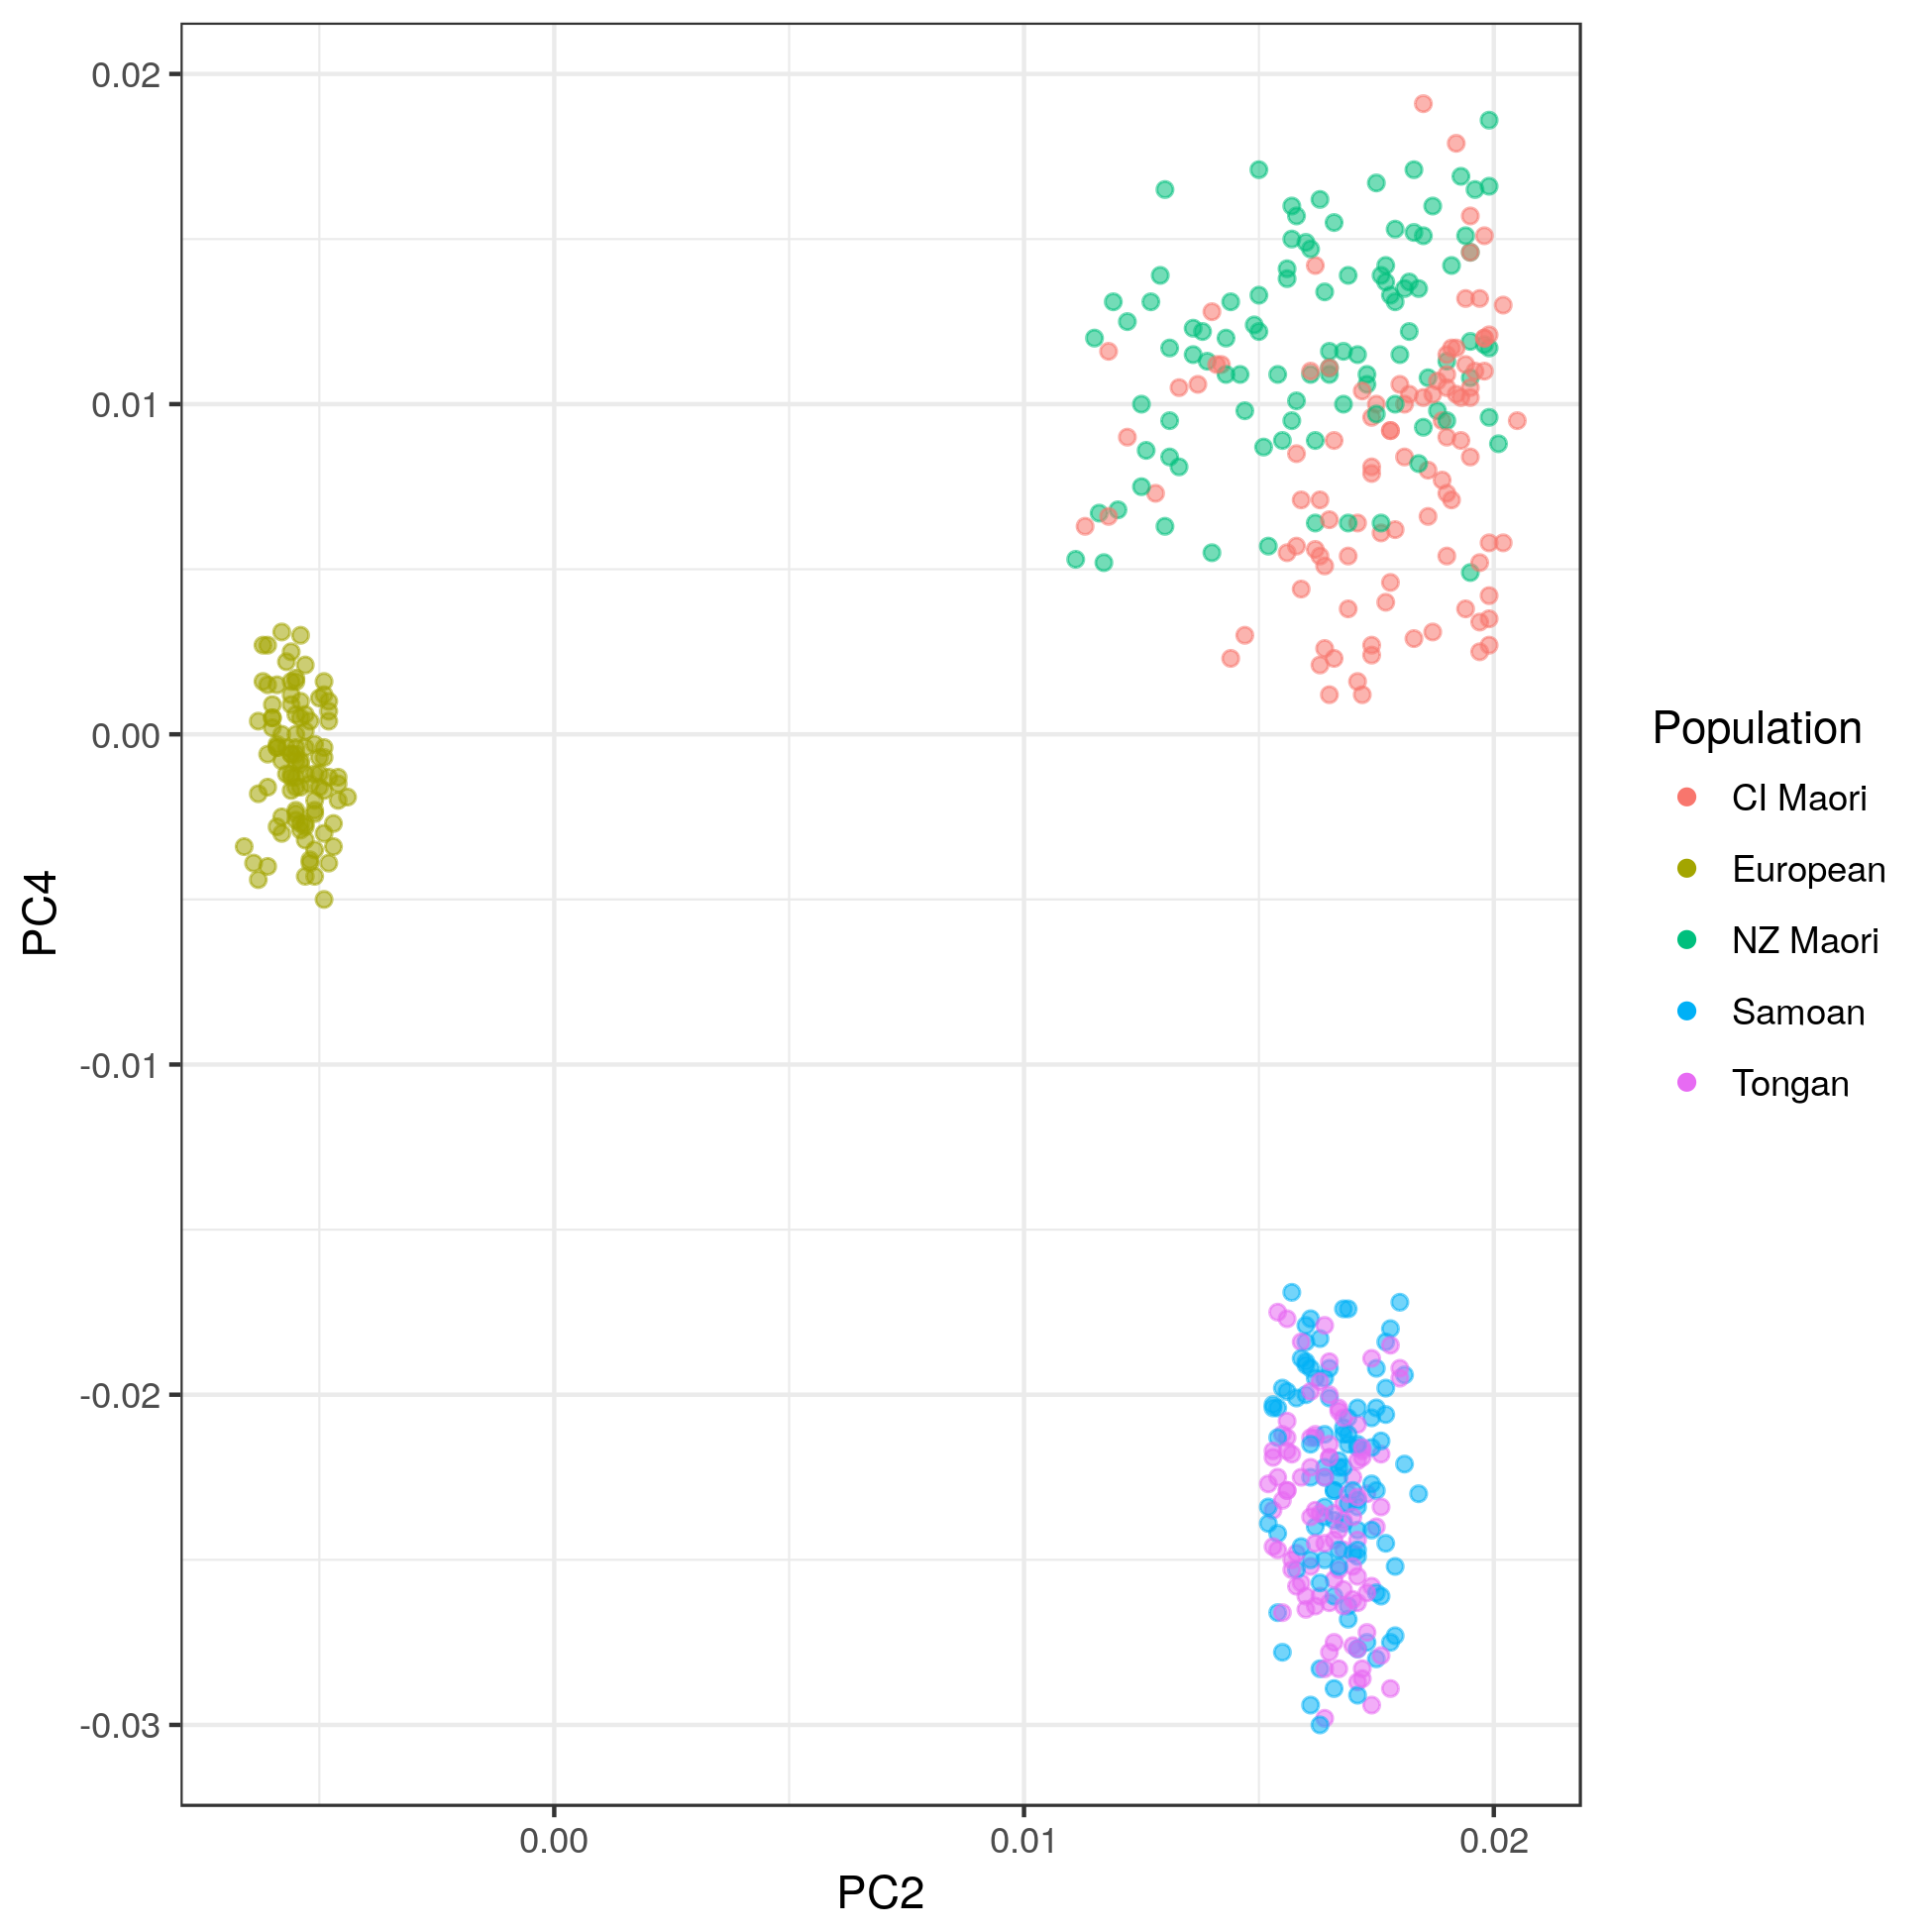
\includegraphics[width=0.7\linewidth]{images/02_methods/pca_plot} 

}

\caption{Principal components 2 and 4 for individuals used in the
selection analysis.}\label{fig:cePCA}
\end{figure}

\subsubsection{Filter individuals and
markers}\label{filter-individuals-and-markers}

To create a data set from which to calculate selection statistics, the
subset of the Genetics of Aotearoa individuals genotyped on the Illumina
CoreExome chip were combined with all of the individuals in the
\gls{1kgp} phase 3 release. This was done in order to have a common set
of markers between all populations, making the populations comparable.
Before the data sets could be combined there were a series of steps that
were performed. The first step (code following) was to keep only the
individuals who had been selected through \gls{pca} and had a genotyping
rate (percentage of all markers with genotypes) of at least 95\%. Due to
software requirements, markers were filtered to remove \glspl{indel} so
that only \glspl{snp} remained.

\begin{Shaded}
\begin{Highlighting}[]
\ExtensionTok{parallel} \StringTok{'}
\StringTok{  plink2 \textbackslash{}}
\StringTok{    --bfile src_data/QC1_7-plus_correctAff \textbackslash{}}
\StringTok{    --recode vcf \textbackslash{}}
\StringTok{    --out QC1_7-plus_correctAff.chr\{\} \textbackslash{}}
\StringTok{    --chr \{\} \textbackslash{}}
\StringTok{    --remove src_data/QC1_7-BlanketExclusions.txt \textbackslash{}}
\StringTok{    --keep coreExome_selection_keep_ids.txt \textbackslash{}}
\StringTok{    --allow-no-sex \textbackslash{}}
\StringTok{    --snps-only no-DI \textbackslash{}}
\StringTok{    --geno 0.95}
\StringTok{    '}\NormalTok{ ::: }\VariableTok{$(}\FunctionTok{seq}\NormalTok{ 1 22}\VariableTok{)}
\end{Highlighting}
\end{Shaded}

The second step was to ensure that all the CoreExome markers were
normalised against the hs37d5 human reference. This was to make sure the
reference (REF) and alternative (ALT) alleles would match with the
\gls{1kgp} phase 3 for a successful merge after phasing and subject
selection. SHAPEIT2 was then used to find \gls{snp} alleles that
disagreed with the \gls{1kgp} haplotype reference and phase the
CoreExome markers. This step (code following) also reduced markers to
baillelic positions and removed duplicate positions.

\begin{Shaded}
\begin{Highlighting}[]
\ExtensionTok{parallel} \StringTok{'}
\StringTok{  bcftools norm \textbackslash{}}
\StringTok{    -N \textbackslash{}}
\StringTok{    --rm-dup any \textbackslash{}}
\StringTok{    --check-ref s \textbackslash{}}
\StringTok{    -f hs37d5.fa \textbackslash{}}
\StringTok{    -O v QC1_7-plus_correctAff.chr\{\}.vcf | \textbackslash{}}
\StringTok{  bcftools view \textbackslash{}}
\StringTok{    -m 2 \textbackslash{}}
\StringTok{    -M 2  \textbackslash{}}
\StringTok{    -O z \textbackslash{}}
\StringTok{    -o QC1_7-plus_correctAff_norm.chr\{\}.vcf.gz \textbackslash{}}
\StringTok{  '}\NormalTok{ ::: }\VariableTok{$(}\FunctionTok{seq}\NormalTok{ 1 22}\VariableTok{)}
\end{Highlighting}
\end{Shaded}

After normalisation, the \gls{vcf} files were phased using the 1000
Genomes Project phase 3 reference haplotypes as described in section
\ref{phase}.

\subsubsection{Merge genotypes}\label{merge-genotypes}

In order to efficiently merge the data sets, the intersection of the
markers from the \gls{1kgp} dataset and the CoreExome dataset was found.
This was done by extracting the marker positions and alleles from the
CoreExome data and then matching these to the marker positions extracted
from the \gls{1kgp} phase 3. The \gls{1kgp} phase 3 markers were also
filtered to remove non-biallelic \glspl{snp}. The following code
demonstrates these steps.

\begin{Shaded}
\begin{Highlighting}[]
\CommentTok{# extract markers from core exome}
\ExtensionTok{parallel} \StringTok{'}
\StringTok{  zgrep \textbackslash{}}
\StringTok{    -v "^#" QC1_7-plus_correctAff_norm.chr\{\}.phased.vcf.gz |\textbackslash{}}
\StringTok{    cut -f1,2,4,5 > coreExome_chr\{\}_biallelic_markers.txt }
\StringTok{    '}\NormalTok{ ::: }\VariableTok{$(}\FunctionTok{seq}\NormalTok{ 1 22}\VariableTok{)}

\CommentTok{# extract 1000 Genomes markers}
\ExtensionTok{parallel} \StringTok{'}
\StringTok{  bcftools view \textbackslash{}}
\StringTok{    -O v \textbackslash{}}
\StringTok{    -m 2 \textbackslash{}}
\StringTok{    -M 2 \textbackslash{}}
\StringTok{    -v snps \textbackslash{}}
\StringTok{    -o - \textbackslash{}}
\StringTok{    ALL.chr\{\}.phase3_shapeit2_mvncall_integrated_v5a.20130502.genotypes.vcf.gz |\textbackslash{}}
\StringTok{  grep -v "^#" |\textbackslash{}}
\StringTok{  cut -f 1,2,4,5 > 1kgp_chr\{\}_biallelic_markers.txt }
\StringTok{  '}\NormalTok{ ::: }\VariableTok{$(}\FunctionTok{seq}\NormalTok{ 1 22}\VariableTok{)}
\end{Highlighting}
\end{Shaded}

An R script (below) was created in order to merge the two marker lists
based on chromosome position and the reference and alternate alleles.

\begin{Shaded}
\begin{Highlighting}[]
\CommentTok{# create list of markers present in CoreExome data}
\NormalTok{ce_markers <-}\StringTok{ }\KeywordTok{data.frame}\NormalTok{()}
\NormalTok{tmp_list <-}\StringTok{ }\KeywordTok{list}\NormalTok{()}
\ControlFlowTok{for}\NormalTok{(i }\ControlFlowTok{in} \DecValTok{1}\OperatorTok{:}\DecValTok{22}\NormalTok{)\{}
\NormalTok{  tmp_list[[i]] <-}\StringTok{ }\KeywordTok{read.table}\NormalTok{(}\DataTypeTok{file =} \KeywordTok{paste0}\NormalTok{(}
    \StringTok{'NZ_coreExome/coreExome_chr'}\NormalTok{,}
\NormalTok{    i,}\StringTok{'_biallelic_markers.txt'}\NormalTok{), }\DataTypeTok{header=}\OtherTok{FALSE}\NormalTok{)}
\NormalTok{\}}
\NormalTok{ce_markers <-}\StringTok{ }\KeywordTok{do.call}\NormalTok{(rbind, tmp_list)}

\CommentTok{# create list of markers present in 1KGP data}
\NormalTok{kg_markers <-}\StringTok{ }\KeywordTok{data.frame}\NormalTok{()}
\NormalTok{tmp_list2 <-}\StringTok{ }\KeywordTok{list}\NormalTok{()}
\ControlFlowTok{for}\NormalTok{(i }\ControlFlowTok{in} \DecValTok{1}\OperatorTok{:}\DecValTok{22}\NormalTok{)\{}
\NormalTok{  tmp_list2[[i]] <-}\StringTok{ }\KeywordTok{read.table}\NormalTok{(}\DataTypeTok{file=} \KeywordTok{paste0}\NormalTok{(}
    \StringTok{'1kgp_chr'}\NormalTok{,i,}\StringTok{'_biallelic_markers.txt'}\NormalTok{), }
    \DataTypeTok{header=}\OtherTok{FALSE}\NormalTok{)}
  \CommentTok{# find the markers in common between CoreExome and 1KGP}
\NormalTok{  tmp_list2[[i]] <-}\StringTok{  }\NormalTok{tmp_list2[[i]][ tmp_list2[[i]][,}\DecValTok{2}\NormalTok{] }\OperatorTok\StringTok{ }\NormalTok{tmp_list[[i]][,}\DecValTok{2}\NormalTok{],]}
\NormalTok{\}}
\NormalTok{kg_markers <-}\StringTok{ }\KeywordTok{do.call}\NormalTok{(rbind, tmp_list2)}
\NormalTok{ce_kg <-}\StringTok{ }\KeywordTok{merge}\NormalTok{(ce_markers, kg_markers, }\DataTypeTok{by =} \KeywordTok{c}\NormalTok{(}\StringTok{"V1"}\NormalTok{,}\StringTok{"V2"}\NormalTok{,}\StringTok{"V3"}\NormalTok{,}\StringTok{"V4"}\NormalTok{))}

\CommentTok{# write out the common markers}
\KeywordTok{write.table}\NormalTok{(}\DataTypeTok{file =} \StringTok{'ce_1kg_matched_markers.txt'}\NormalTok{, ce_kg[,}\KeywordTok{c}\NormalTok{(}\DecValTok{1}\NormalTok{,}\DecValTok{2}\NormalTok{)], }
            \DataTypeTok{row.names =} \OtherTok{FALSE}\NormalTok{, }\DataTypeTok{col.names=}\OtherTok{FALSE}\NormalTok{, }\DataTypeTok{quote=}\OtherTok{FALSE}\NormalTok{)}
\end{Highlighting}
\end{Shaded}

Once the combined marker list was created, both the CoreExome and
\gls{1kgp} data sets had markers filtered to match this consensus set.
The code for marker filtering of the \gls{vcf} files and subsequent
merge is shown below.

\begin{Shaded}
\begin{Highlighting}[]
\CommentTok{# filter 1000 Genomes markers}
\ExtensionTok{parallel} \StringTok{'}
\StringTok{  bcftools view }
\StringTok{    -R ../ce_1kg_matched_markers.txt \textbackslash{}}
\StringTok{    -O z \textbackslash{}}
\StringTok{    -m 2 \textbackslash{}}
\StringTok{    -M 2 \textbackslash{}}
\StringTok{    -v snps \textbackslash{}}
\StringTok{    -o ALL.chr\{\}.phase3_shapeit2_mvncall_integrated_v5a.20130502.matched.vcf.gz \textbackslash{}}
\StringTok{    ALL.chr\{\}.phase3_shapeit2_mvncall_integrated_v5a.20130502.genotypes.vcf.gz }
\StringTok{  '}\NormalTok{ ::: }\VariableTok{$(}\FunctionTok{seq}\NormalTok{ 1 22}\VariableTok{)}

\CommentTok{# filter coreExome markers}
\ExtensionTok{parallel} \StringTok{'}
\StringTok{  bcftools view \textbackslash{}}
\StringTok{    -R ../ce_1kg_matched_markers.txt \textbackslash{}}
\StringTok{    -O z \textbackslash{}}
\StringTok{    -m 2 \textbackslash{}}
\StringTok{    -M 2 \textbackslash{}}
\StringTok{    -v snps \textbackslash{}}
\StringTok{    -o NZ_coreExome.chr\{\}.norm.phased.matched.vcf.gz \textbackslash{}}
\StringTok{    QC1_7-plus_correctAff_norm.chr\{\}.phased.vcf.gz }
\StringTok{  '}\NormalTok{ ::: }\VariableTok{$(}\FunctionTok{seq}\NormalTok{ 1 22}\VariableTok{)}

\CommentTok{# merge 1kgp and nz coreexome}
\ExtensionTok{parallel} 
  \StringTok{'bcftools merge \textbackslash{}}
\StringTok{    -O z \textbackslash{}}
\StringTok{    -o NZ_1KGP.chr\{\}.phased.vcf.gz \textbackslash{}}
\StringTok{    ALL.chr\{\}.phase3_shapeit2_mvncall_integrated_v5a.20130502.matched.vcf.gz \textbackslash{}}
\StringTok{    NZ_coreExome/NZ_coreExome.chr\{\}.norm.phased.matched.vcf.gz }
\StringTok{  '}\NormalTok{ ::: }\VariableTok{$(}\FunctionTok{seq}\NormalTok{ 1 22}\VariableTok{)}
\end{Highlighting}
\end{Shaded}

Sample identifiers were then updated to match the panel file that
described the population and super population an individual belonged to.
The following code applies this step to each merged \gls{vcf} file.

\begin{Shaded}
\begin{Highlighting}[]
\CommentTok{# Combine FID and IID of CoreExome samples so they match the panel file}
\KeywordTok{for} \ExtensionTok{i}\NormalTok{ in }\VariableTok{$(}\FunctionTok{seq}\NormalTok{ 1 22}\VariableTok{)}
\KeywordTok{do} 
  \FunctionTok{zcat}\NormalTok{ NZ_1KGP.chr}\VariableTok{$i}\NormalTok{.phased.vcf.gz }\KeywordTok{|\textbackslash{}}
  \FunctionTok{head}\NormalTok{ -1000 }\KeywordTok{|\textbackslash{}}
  \FunctionTok{grep} \StringTok{'^#CHROM'} \KeywordTok{|\textbackslash{}}
  \FunctionTok{cut}\NormalTok{ -f10- }\KeywordTok{|\textbackslash{}}
  \FunctionTok{tr} \StringTok{'\textbackslash{}t'} \StringTok{'\textbackslash{}n'} \KeywordTok{|\textbackslash{}}
  \FunctionTok{awk}\NormalTok{ -F }\StringTok{"_"} \StringTok{'\{if(NF ==1 ) \{print $1 "\textbackslash{}t" $1\}else\{print $1"_"$2"\textbackslash{}t" $2\}\}'} \KeywordTok{|\textbackslash{}}
  \ExtensionTok{bcftools}\NormalTok{ reheader \textbackslash{}}
\NormalTok{    -s /dev/stdin/ \textbackslash{}}
\NormalTok{    -o NZ_1KGP.chr}\VariableTok{$i}\NormalTok{.phased.sample_updated.vcf.gz \textbackslash{}}
\NormalTok{    NZ_1KGP.chr}\VariableTok{$i}\NormalTok{.phased.vcf.gz}
\KeywordTok{done}
\end{Highlighting}
\end{Shaded}

\subsection{UK Biobank}\label{ukbbdata}

The UK Biobank is a collection of 500,000 individuals, mostly of
European ancestry from around the United Kingdom, and aged between 40
and 69. It consists of genetic, health, and lifestyle information. The
interim release dataset (approval number 12611) was downloaded in
November 2015 and contained genotypes for 152,249 individuals. Gout
affection was determined by self-report, or self-reported use of urate
lowering therapy, or an International Classification of Diseases, Tenth
Revision (ICD-10) code for gout (M10, including sub-codes). The dataset
was also filtered to individuals with a self-reported ethnic background
of British, Irish, or `any other white background'. Individuals were
removed who had a mismatch between self-reported sex and genetic sex, or
whose samples failed genotype quality control. The remaining individuals
were eligible for inclusion in the \gls{gwas} performed in section
\ref{ukbbgwas}.

\subsection{Reference datasets}\label{reference-datasets}

Table \ref{tab:refDatasets} provides the name of the dataset, the date
it was accessed, and the URL from which the dataset was downloaded.
These datasets were incorporated into many of the analysis steps.

\begin{longtable}[]{@{}lll@{}}
\caption{\label{tab:refDatasets} Reference Datasets}\tabularnewline
\toprule
\begin{minipage}[b]{0.24\columnwidth}\raggedright\strut
Name\strut
\end{minipage} & \begin{minipage}[b]{0.20\columnwidth}\raggedright\strut
Date\strut
\end{minipage} & \begin{minipage}[b]{0.47\columnwidth}\raggedright\strut
URL\strut
\end{minipage}\tabularnewline
\midrule
\endfirsthead
\toprule
\begin{minipage}[b]{0.24\columnwidth}\raggedright\strut
Name\strut
\end{minipage} & \begin{minipage}[b]{0.20\columnwidth}\raggedright\strut
Date\strut
\end{minipage} & \begin{minipage}[b]{0.47\columnwidth}\raggedright\strut
URL\strut
\end{minipage}\tabularnewline
\midrule
\endhead
\begin{minipage}[t]{0.24\columnwidth}\raggedright\strut
1000 Genomes Project Phase 3 release 5\strut
\end{minipage} & \begin{minipage}[t]{0.20\columnwidth}\raggedright\strut
20 Mar 2017\strut
\end{minipage} & \begin{minipage}[t]{0.47\columnwidth}\raggedright\strut
\url{http://ftp.1000genomes.ebi.ac.uk/vol1/ftp/release/20130502/}\strut
\end{minipage}\tabularnewline
\begin{minipage}[t]{0.24\columnwidth}\raggedright\strut
1000 Genomes Phase 3 phased haplotypes\strut
\end{minipage} & \begin{minipage}[t]{0.20\columnwidth}\raggedright\strut
14 Dec 2014\strut
\end{minipage} & \begin{minipage}[t]{0.47\columnwidth}\raggedright\strut
\url{https://mathgen.stats.ox.ac.uk/impute/1000GP_Phase3.html}\strut
\end{minipage}\tabularnewline
\begin{minipage}[t]{0.24\columnwidth}\raggedright\strut
Human Genome Reference FASTA\strut
\end{minipage} & \begin{minipage}[t]{0.20\columnwidth}\raggedright\strut
5 Aug 2014\strut
\end{minipage} & \begin{minipage}[t]{0.47\columnwidth}\raggedright\strut
\url{ftp://ftp.1000genomes.ebi.ac.uk:21/vol1/ftp/technical/reference/phase2_reference_assembly_sequence/hs37d5.fa.gz}\strut
\end{minipage}\tabularnewline
\begin{minipage}[t]{0.24\columnwidth}\raggedright\strut
Human Ancestral Allele FASTA\strut
\end{minipage} & \begin{minipage}[t]{0.20\columnwidth}\raggedright\strut
6 Aug 2014\strut
\end{minipage} & \begin{minipage}[t]{0.47\columnwidth}\raggedright\strut
\url{ftp://ftp.ensembl.org/pub/release-66/fasta/ancestral_alleles/homo_sapiens_ancestor_GRCh37_e66.tar.bz}\strut
\end{minipage}\tabularnewline
\bottomrule
\end{longtable}

\chapter{Positive Selection in Polynesian
Populations}\label{selectionResults}

\glsresetall

In this chapter I investigate regions of the genome that exhibit
signatures of selection in Polynesian populations, with a particular
focus on loci associated with serum urate levels and metabolic
conditions.

\section{Introduction}\label{introduction-1}

At the turn of the millennium the draft reference human genome was
released \citep{Lander2001}. Following from this, there were a number of
large projects to characterise human variation and diversity. The first
project was the HapMap project \citep{Hapmap2005} and was based on
\gls{snp} array data. This was followed by the 1000 Genomes Project
\citep{1KGP2010, 1KGP2012, 1KGP2015snp} which was the first large
project to be based on whole-genome (re)sequence data. Alongside these
variation projects were a few projects that aimed to focus on the
genomic diversity of humans, such as the Human Genome Diversity Project
\citep{Cann2002, Rosenburg2002}, and later the Simons Genome Diversity
Project \citep{Mallick2016}.

Over the last decade there has been a steady flow of studies on
genome-wide selection
\citep{sabeti2006positive, voight2006map, tang2007new, Coop2009, pickrell2009signals, Grossman2010}.
The main population samples for this have been part of the 1000 Genomes
Project, which sampled over 2500 individuals for full genome
(re)sequencing from five `super' population groups \citep{1KGP2015snp}.
The five super populations cover each of the geographical regions of
Africa, Europe, East Asia, South Asia, and the Americas. This dataset,
while capturing a large representation of the human population
variation, does not have representation for the populations of
Polynesia.

\subsection{Positive selection}\label{positive-selection}

\subsection{Selection in Polynesian
populations}\label{selection-in-polynesian-populations}

Projects to capture the genetic diversity of humans have sampled
populations worldwide, but outside the populations sampled by the 1000
Genomes Project, the population sample sizes have been small
\citep{Cann2002, Rosenburg2002, Mallick2016}. Past studies that have
included Oceanic populations have had minimal representation of
Polynesian populations, for example, \citet{Kimura2008} only had 24
Tongan individuals. The latest project for human diversity, the Simons
Human Diversity Project, did include New Zealand M\tex{\={a}}ori but
they were only represented by a single individual and did not feature in
many of the analyses \citep{Mallick2016}.

More recently there have been studies that have looked at selection in
Polynesian populations but with a focus on a few candidate loci, not at
a genome-wide scale \citep{Myles2011, Cadzow2016, Minster2016}. The main
feature of these studies has been the investigation of ``thrifty
genes''.

\subsubsection{Thrifty gene hypothesis}\label{thrifty-gene-hypothesis}

The ``Thrifty genotype hypothesis'' was originally hypothesised by
\citet{Neel1962}, whereby it was posed there must be a genetic advantage
to a disease, given what should be a strong selection pressure against
it, for it to continue to have a high prevalence - referring to
diabetes. In the Polynesian context, this hypothesis has been invoked in
an attempt to explain the higher prevalence of metabolic related
diseases such as \gls{t2d} and obesity \citep{Myles2011, Minster2016}.
However, there are several refutations of the thrifty genotype for
Polynesian populations as fitting a particular narrative
\citep{Gosling2014, Gosling2015, Cadzow2016}. An alternative to the
`thrifty-gene' hypothesis is that the link between metabolic diseases
and the innate immune system, susceptibility of populations to metabolic
disease might be due to selective pressure from infectious disease, such
as malaria \citep{Gosling2015}. Uricase, the enzyme for metabolising
urate, was lost through multiple mutations - a reduction in promoter
activity followed by two further loss of function mutations and occurred
before the divergence of humans from the great apes \citep{Kratzer2014}.
The evolutionary history of uricase however has also been described as
``the original thrifty-gene'' \citep{Kratzer2014}.

\subsection{Selection in urate and
gout}\label{selection-in-urate-and-gout}

The benefits of urate include the its ability to increase blood pressure
and it is thought to have helped early hominins to stand upright
\citep{Watanabe2002} and increase blood flow to the brain. Serum urate
is also a potent anti-oxidant which accounts for \textgreater{}50\% of
the anti-oxidant activity of the blood
\citep{Glantzounis2005, Parmar2009}. Mono-sodium urate crystals that
form in conditions of elevated urate are a potent adjuvant for the
immune system and enhances the immune response
\citep{Ames1981, Opitz2009}. Uric acid has also been identified as being
an important part of the malarial response, contributing to cytokine
secretion and response of dendritic and T-cells
\citep{GallegoDelgado2014}.

An increased level of urate in the blood is called hyperuricaemia and is
causal of gout \citep{Choi2005a}. The prevalence of hyperuricaemia in
Polynesian populations is higher than many other populations
\citep{Gosling2014}, and co-morbid with it are higher prevalences of the
co-morbidities of gout, diabetes, obesity, dyslipidaemia, kidney
disease, and \gls{cvd} \citep{Winnard2013}. In New Zealand, gout
prevalence is \textasciitilde{}3.1\%, however, prevalence in
M\tex{\={a}}ori and Pacific peoples is 6-8\% with 40\% of individuals
with gout also having diabetes or \gls{cvd} \citep{Winnard2013}. Gout is
an immune response to the monosodium urate crystals that are formed from
the precipitation of urate from the blood, with hyperuricaemia being a
prerequisite for the formation of these crystals \citep{Merriman2011a}.

Hyperuricaemia has two main components: overproduction of urate, and
under-excretion. Overproduction is influenced by diet, such as high
purine or fructose content, or increased cell turnover as observed in
cancer, or under genetic control. Under-excretion is the main cause of
hyperuricaemia, caused by either increased reabsorption or decreased
secretion. The kidneys are the organ where the majority of secretion and
excretion of urate is performed, with about 90\% of urate being
reabsorbed \citep{Kutzing2008}. In the proximal tubule, on the apical
membrane, the urate transporters of URAT1 (\emph{SLC22A12}), OAT4
(\emph{SLC22A11}), and GLUT9 (\emph{SLC2A9}) reabsorb urate, whereas
ABCC4, NPT4 (\emph{SLC17A3}), and NPT1 (\emph{SLC17A1}) are responsible
for secretion (Figure \ref{fig:urateTransporters}) \citep{Mandal2015}.
On the basolateral membrane, OAT1-3 (\emph{SLC22A6-8}), increase
intracellular uric acid, but GLUT9 moves uric acid from intracellular to
extracellular \citep{Mandal2015}. The ATP powered transporter ABCG2 is
responsible for excretion of urate in the gut and there are \glspl{snp}
that lead to a reduction of function in ABCG2 in all populations (Figure
\ref{fig:urateTransporters}) \citep{Phipps-Green2010, Cleophas2017}.
Together the genes \emph{SLC2A9} and \emph{ABCG2} account for 3.4\% of
the genetic variability of urate \citep{Kottgen2013}.

\begin{figure}
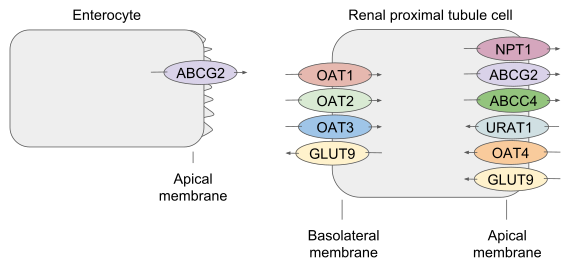
\includegraphics{_bookdown_files/images/03_selectionpipeline/urate_excretion_diagram} \caption[Location of urate transporters of gut and kidney.]{Diagram representing the urate transporters in
the gut (entrocyte) and kidney (renal proximal tubule cell). Direction
of urate movement is indicated by arrows. Adapted from
\citet{Major2018}.}\label{fig:urateTransporters}
\end{figure}






From previous studies there is prior evidence of selection at urate
associated loci \citep{Grossman2013, Zhang2013a, Ramos2017}. In the
review from \citet{Ramos2017} on natural selection in rheumatic disease,
one of the main loci for gout, \emph{SLC2A9}, in the \gls{yri}
population was reported as having been selected. The region of
\emph{BCAS3} and \emph{NACA2} also had evidence, originally found by
\citet{Grossman2013} in the Asian population from the HapMap project
data. \citet{Zhang2013a} had evidence for the urate-associated loci of
\emph{ATXN2} (rs653178) and \emph{RREB1} (rs675209) having undergone
selection when using a F\textsubscript{ST}-based method. The
co-morbidities of hyperuricaemia also show signs of selection, with loci
associated with \gls{t2d} having been reported as having undergone
selection
\citep{voight2006map, pickrell2009signals, Grossman2010, Grossman2013}.
Most recently a Samoan specific variant in \emph{CREBRF} that is
protective for \gls{t2d} but causal for obesity has also been identified
as having evidence of selection in the Samoan population
\citep{Minster2016}.

\subsection{Objectives}\label{objectives}

The objectives of this chapter are to:

\begin{itemize}
\tightlist
\item
  Investigate regions that are under selection in Polynesian
  populations.
\item
  Investigate regions previously associated with urate, \gls{t2d},
  obesity, kidney disease, and metabolic syndrome for signatures of
  selection.
\end{itemize}

\section{Methods}\label{methods}

The choice of individuals, and preliminary data preparation for the
selection data set is detailed in section \ref{selectionDataset}. It
consisted of combining 500 individuals (100 per population for each of
\gls{nzm}, \gls{cim}, \gls{sam}, \gls{ton}, and \gls{nzc}) from the
Genetics of Gout in Aotearoa study, who had been genotyped on the
Illumina CoreExome v24 \gls{snp} array with 2504 individuals from the
1000 Genomes Project.

\subsection{Calculation of selection and neutrality
statistics}\label{calcSel}

The R package PopGenome v2.2.3 \citep{Pfeifer2014} was used to calculate
the site-frequency spectrum statistics \gls{td}, \gls{fwh}, \gls{flf},
\gls{ze}, and F\textsubscript{ST} over non-overlapping windows of 10 kb
(see section \ref{popgenomeMethods} for further details). Except for
F\textsubscript{ST}, the empirical distribution for each population was
used to create an upper and a lower significance threshold. The lower
threshold was the 1\textsuperscript{st} percentile and less than zero.
The upper significance threshold was the 99\textsuperscript{th}
percentile and greater than zero. Contiguous regions of score depression
or elevation were created using a rolling window approach, whereby a
condition of 15 or more windows out of a minimum of 20 consecutive 10 kb
windows were required to have met a significance threshold in the same
tail of the distribution. These represent extended regions of the genome
and can be indicative of a selective sweep \citep{Carlson2005}.

The \gls{ihs}, \gls{nsl}, and \gls{xpehh} were calculated and normalised
using selscan v1.1.0b \citep{Szpiech2014} as part of the selectionTools
1.1 \citep{Cadzow2014}, pipeline as detailed in section
\ref{selectionTools}. The default setting was used which was a maximum
gap extension of 200 kb. Significance was defined as
\textbar{}value\textbar{} \textgreater{} 2.6 which was equivalent to the
most extreme \textasciitilde{}1\% of values after normalisation using
frequency bins of 0.05.

\subsection{Pathway enrichment
analysis}\label{pathway-enrichment-analysis}

Pathway enrichment analysis was performed by taking genes that
intersected the 1\textsuperscript{st} percentile windows for the
\glsdesc{sfs}-based statistics that also had a value \textless{} 0, or
genes that had a significant marker for \gls{ihs} or \gls{nsl} and
inputting them into Enrichr\footnote{\url{http://amp.pharm.mssm.edu/Enrichr/}
  accessed 22 November 2017} \citep{Chen2013b, Kuleshov2016} and
exporting the KEGG 2016 pathway table.




\section{Results}\label{results}

Results will be split into two themes, the first will be regions of the
genome that show evidence of selection in the Polynesian populations.
This theme will initially cover the results of the Polynesian
populations as a combined group, and then results that were specific to
individual populations. The second theme will look specifically at
selection of urate and associated loci in Polynesian populations. For
reporting, there will be a focus on the 1\textsuperscript{st}
percentile/lower tail for the intra-population statistics as this is the
distribution end that corresponds with positive selection.

\subsection{False discovery rate of windowed
statistics}\label{fdrresults}

\begin{table}

\caption{\label{tab:fdrpol}\label{tab:fdrpol} False discovery rate for windowed frequency spectrum based intra-population statistics by population.}
\centering
\begin{threeparttable}
\begin{tabular}[t]{lrlrl}
\toprule
\multicolumn{1}{c}{} & \multicolumn{2}{c}{Lower tail} & \multicolumn{2}{c}{Upper tail} \\
\cmidrule(l{2pt}r{2pt}){2-3} \cmidrule(l{2pt}r{2pt}){4-5}
Population & Percentile & FDR (95\% CI) & Percentile & FDR (95\% CI)\\
\midrule
\addlinespace[0.3em]
\multicolumn{5}{l}{\textbf{Fay and Wu's H}}\\
\hspace{1em}CIM & 0.06 & 0.059 (0.051, 0.071) & 99.4 & 0.571 (0.532, 0.609)\\
\hspace{1em}NZM & 0.07 & 0.066 (0.057, 0.076) & 99.4 & 0.585 (0.538, 0.625)\\
\hspace{1em}SAM & 0.06 & 0.056 (0.049, 0.065) & 99.4 & 0.570 (0.524, 0.615)\\
\hspace{1em}TON & 0.05 & 0.050 (0.043, 0.059) & 99.4 & 0.589 (0.546, 0.626)\\
\addlinespace[0.3em]
\multicolumn{5}{l}{\textbf{Fu and Li's F}}\\
\hspace{1em}CIM & 0.20 & 0.181 (0.161, 0.206) & 99.6 & 0.348 (0.305, 0.389)\\
\hspace{1em}NZM & 0.20 & 0.170 (0.152, 0.193) & 99.6 & 0.371 (0.327, 0.423)\\
\hspace{1em}SAM & 0.20 & 0.184 (0.167, 0.205) & 99.5 & 0.436 (0.386, 0.484)\\
\hspace{1em}TON & 0.20 & 0.191 (0.175, 0.220) & 99.5 & 0.490 (0.436, 0.554)\\
\addlinespace[0.3em]
\multicolumn{5}{l}{\textbf{Tajima's D}}\\
\hspace{1em}CIM & 0.03 & 0.028 (0.023, 0.034) & 99.8 & 0.165 (0.147, 0.189)\\
\hspace{1em}NZM & 0.04 & 0.037 (0.032, 0.045) & 99.8 & 0.174 (0.156, 0.194)\\
\hspace{1em}SAM & 0.02 & 0.019 (0.016, 0.024) & 99.8 & 0.191 (0.169, 0.219)\\
\hspace{1em}TON & 0.03 & 0.026 (0.022, 0.031) & 99.8 & 0.188 (0.165, 0.213)\\
\addlinespace[0.3em]
\multicolumn{5}{l}{\textbf{Zeng's E}}\\
\hspace{1em}CIM & 2.00 & 1.000 (1.000, 1.000) & 99.5 & 0.436 (0.405, 0.472)\\
\hspace{1em}NZM & 2.00 & 1.000 (1.000, 1.000) & 99.5 & 0.434 (0.401, 0.470)\\
\hspace{1em}SAM & 2.00 & 1.000 (1.000, 1.000) & 99.6 & 0.389 (0.361, 0.422)\\
\hspace{1em}TON & 2.00 & 1.000 (1.000, 1.000) & 99.6 & 0.389 (0.362, 0.423)\\
\bottomrule
\end{tabular}
\begin{tablenotes}
\item Percentile is the more conservative FDR quantile bin of the permuted data that was equivalent to either the 1st (lower tail) or 99th (upper tail) percentile in the observed data.
\end{tablenotes}
\end{threeparttable}
\end{table}

In order to control for false positives, the empirical \gls{fdr} was
calculated for \gls{td}, \gls{flf}, \gls{fwh}, and \gls{ze}. To
calculate the \gls{fdr}, 5000 permutations of the genotype data were
performed, each randomly shuffling the genotypes of markers by marker
position (i.e.~shuffling rows only). This process re-defined the marker
composition of each window, requiring new selection statistics to be
calculated for each window. This procedure therefore, generated a new
distribution for values of each selection statistic (per permutation)
under the null hypothesis of no association between marker genotype and
genomic position. A similar method was used by Teshima and colleagues
\citeyearpar{Teshima2006}. For each permutation, for each statistic, the
values for quantile `bins' were calculated for both tails of the
distribution. The `bins' ranged from 0.01 to 0.1\% in 0.01 increments,
0.1 to 1\% in 0.1\% increments, 1 to 5\% in 1\% increments, and 10\%.
The median and 95\% confidence intervals were calculated for the values
of the quantile `bins' across the permutations (i.e., the median,
2.5\textsuperscript{th} and 97.5\textsuperscript{th} percentiles for the
values of the 1\textsuperscript{st} percentile bin from all
permutations). The enrichment for each quantile bin was then calculated
by comparing the number of windows that were observed in the data
compared to the number expected from the permutations. \Gls{fdr} was
then estimated by using the value for the 1\textsuperscript{st} or
99\textsuperscript{th} percentile and finding the nearest conservative
quantile bin using the median, that was either larger for the lower
tail, or smaller for the upper tail and taking the inverse of enrichment
for the bin (Table \ref{tab:fdrpol}). As a result, the estimate will be
conservative compared to the true \gls{fdr} but will still maintain
\gls{fdr} control.

The \gls{fdr} for \gls{ze} was 1.0 for all Polynesian populations in the
lower end of the distribution and the 1\textsuperscript{st} percentile
of the data fell within the 2\textsuperscript{nd} percentile bin from
the permutations. This means that the 1\textsuperscript{st} percentile
threshold from the observed \gls{ze} fell between the
1\textsuperscript{st} and 2\textsuperscript{nd} percentile of the null
distribution and was entirely within the 95\% confidence interval.
Whereas, for \gls{td} and \gls{fwh} the maximum quantile bin for the
Polynesian populations in the lower tail was 0.07\% (\gls{nzm}), with
the maximum upper confidence interval being 0.076 (\gls{nzm}). For the
purpose of reporting on individual statistics, a threshold of 0.1 was
applied, to reduce the expected false positive rate to be less than 1 in
10 on average. \Gls{flf} and \gls{ze} both had an \gls{fdr} above this
threshold for the Polynesian populations and will be reported on only as
additional evidence when they overlap with other results or were in a
region of contiguously depressed score (section \ref{calcSel}).

\subsection{Comparison with prior publications}\label{priorPubs}

The selection and neutrality statistics that were in the
1\textsuperscript{st} percentile and \textless{} 0 were compared to
regions and genes identified in \citet{Hider2013} for \gls{eas} and
\citet{Jonnalagadda2017} for \gls{sas} as these papers had used a
similar, but not identical methodology to identify regions under
selection. \citet{Hider2013} investigated selection in the East Asian
populations (\gls{chb}, \gls{chs}, and \gls{jpt}) of the 1000 Genomes
Project in the Phase 1 release. For this they used a non-overlapping
window size of 25 kb and excluded windows with less than 10 segregating
sites and then looked at the top 1\% of results. They reported regions
that were significant for \gls{td}, \gls{fwh}, \gls{flf}, and \gls{ihs}.
Comparing the regions from \citet{Hider2013} with regions that met the
significance threshold for this project there were 118 of 206 regions
for \gls{td}, 15 of 151 for \gls{fwh}, 83 of 255 for \gls{flf}, and 5 of
85 for \gls{ihs} (Table \ref{tab:hiderRegionsFound}).

Of the genes reported in \citet{Jonnalagadda2017}, there were 2 of 5 for
\gls{td} (\emph{DST} and \emph{SLC24A5}), 0 of 5 for \gls{fwh}, and 2 of
5 for \gls{ihs} (\emph{TYR} and \emph{ADAM17}) that were also
significant in this project. \citet{Jonnalagadda2017} used the same
window set up as \citet{Hider2013}, but used the 1000 Genomes Project
Phase 3 release for the \gls{gih} and \gls{itu} populations.

In conjunction with the studies from \citet{Hider2013} and
\citet{Jonnalagadda2017}, \citet{Ramos2017} looked at evidence of
selection in rheumatic disease, including gout, using the \gls{ihs}
results from \citet{voight2006map} from the HapMap phase II dataset.
There were three populations used which were Asian, European, and
African. When comparing the loci reported in \citet{Ramos2017} with the
\gls{ihs} results, here the equivalent populations of \gls{chb} and
\gls{jpt} were used to represent the Asian population, \gls{ceu} for
European, and \gls{yri} for African. Where the population was unknown in
\citet{Ramos2017}, all of the specified populations (\gls{ceu},
\gls{chb}, \gls{jpt}, and \gls{yri}), from the 1000 Genomes Project
individuals were used. Loci reported for European had 47.8\% overlap
with \gls{ceu}. The Asian reported loci matched 31.6\% with \gls{chb}
and \gls{jpt}, and for African, 23.1\% of the reported loci were also
found in \gls{yri}. For the loci reported with an unknown population,
65.0\% were found to match in any of \gls{ceu}, \gls{yri}, \gls{chb}, or
\gls{jpt}.

To supplement the \citet{Ramos2017} \gls{ihs} regions, additional genes
were included from \citet{voight2006map} Table 1 to include genes that
showed evidence of selection across different combinations of the
populations and were not specific to rheumatic disease. The populations
covered by these genes were \gls{ceu}, \gls{chb}, \gls{chs}, \gls{jpt},
and \gls{yri}. The genes included were: \emph{LCT} - specific for
\gls{ceu}; \emph{SLC44A5} - specific for \gls{chb}, \gls{chs}, and
\gls{jpt}; \emph{NCOA1}, \emph{ADCY3} and \emph{SYT1} - specific for
\gls{yri}; \emph{SNTG1} - specific for \gls{ceu}, \gls{chb}, \gls{chs},
\gls{jpt}, and \gls{yri}; and \emph{SPAG4} - specific for \gls{ceu} and
\gls{yri}. All genes except \emph{SPAG4} were positive for significant
\gls{ihs} markers in the corresponding populations they were originally
reported in.

The differences in regions being found as significant can be partially
attributed to the differing window sizes, and the difference between
sequence and chip-based genotyping for \citet{Hider2013} and
\citet{Jonnalagadda2017}, and difference in markers for
\citet{Ramos2017}.

\FloatBarrier

\subsection{Selection in Polynesian populations - genome-wide
analysis}\label{selection-in-polynesian-populations---genome-wide-analysis}

In this subsection results will be presented first for those that were
in common between all Polynesian populations and the sub-groups of East
and West Polynesia. Following this, the results for individual
Polynesian populations will be presented. A complete table of all genes
that had results meeting the various thresholds for the various
statistics used can be found in the Appendix Tables
\ref{tab:intrasfsPol} (\gls{sfs}-based statistics),
\ref{tab:ihsnslPolGenes} (\gls{ihs} and \gls{nsl}), and
\ref{tab:xpehhPolgenes} (\gls{xpehh}).

There were 465 genes that were associated with urate and metabolic
diseases from the \gls{gwas} catalog (see Table \ref{tab:gwascatref} for
references), with 152 having at least a single window from the lower
tail, or \gls{snp} meeting a threshold for a single statistic in the
Polynesian populations. Genes reported here were highlighted based on
three criteria: a significant haplotypic result in multiple Polynesian
populations, or having multiple statistics meeting the significance
threshold in at least a single Polynesian population, or the locus only
having the main significant result in Polynesian populations, with
minimal signal in other populations, that is, multiple significant
markers in Polynesian populations and one or two in other populations.

Each Polynesian population had a similar number of windows in the
1\textsuperscript{st} percentile, except for the Western Polynesian
populations with \gls{ze} where they had up to \textasciitilde{}50\%
less (Table \ref{tab:sfsWindowsTable}). The Eastern Polynesian
populations tended to have more independent non-consecutive regions and
number of genes that were intersected by windows than the Western
Polynesian populations. However, this did not translate into a higher
number of genes that were significant in only a single population. There
were similar numbers of genes that intersected the windows that met the
significance threshold in either distribution tail between the
Polynesian populations of \gls{cim}, \gls{nzm}, \gls{sam}, and
\gls{ton}.

\begin{table}

\caption{\label{tab:sfsWindowsTable}\label{tab:sfsWindowsTable} Number of significant regions and genes in Polynesian populations for the intra population SFS statistics.}
\centering
\resizebox{\linewidth}{!}{
\begin{threeparttable}
\begin{tabular}[t]{lrrrrrrrr}
\toprule
\multicolumn{1}{c}{} & \multicolumn{4}{c}{Lower Tail} & \multicolumn{4}{c}{Upper Tail} \\
\cmidrule(l{2pt}r{2pt}){2-5} \cmidrule(l{2pt}r{2pt}){6-9}
Pop & Windows & Regions (n) & Genes (n) & Pop. Genes (n) & Windows & Regions (n) & Genes (n) & Pop. Genes (n)\\
\midrule
\addlinespace[0.3em]
\multicolumn{9}{l}{\textbf{Tajima's D}}\\
\hspace{1em}CIM & 2420 & 590 & 644 & 40 & 2420 & 963 & 466 & 66\\
\hspace{1em}NZM & 2429 & 577 & 713 & 37 & 2429 & 954 & 436 & 42\\
\hspace{1em}SAM & 2396 & 559 & 537 & 50 & 2396 & 961 & 479 & 75\\
\hspace{1em}TON & 2380 & 561 & 508 & 48 & 2380 & 972 & 512 & 72\\
\addlinespace[0.3em]
\multicolumn{9}{l}{\textbf{Fay and Wu's H}}\\
\hspace{1em}CIM & 2420 & 807 & 460 & 25 & 2420 & 895 & 553 & 57\\
\hspace{1em}NZM & 2429 & 770 & 443 & 20 & 2429 & 916 & 573 & 53\\
\hspace{1em}SAM & 2396 & 766 & 470 & 23 & 2396 & 895 & 565 & 36\\
\hspace{1em}TON & 2380 & 764 & 467 & 41 & 2380 & 879 & 575 & 43\\
\addlinespace[0.3em]
\multicolumn{9}{l}{\textbf{Fu and Li's F}}\\
\hspace{1em}CIM & 2419 & 655 & 805 & 72 & 2420 & 818 & 386 & 32\\
\hspace{1em}NZM & 2429 & 624 & 966 & 92 & 2429 & 797 & 379 & 21\\
\hspace{1em}SAM & 2396 & 620 & 671 & 79 & 2396 & 812 & 458 & 47\\
\hspace{1em}TON & 2380 & 669 & 643 & 96 & 2380 & 782 & 467 & 50\\
\addlinespace[0.3em]
\multicolumn{9}{l}{\textbf{Zeng's E}}\\
\hspace{1em}CIM & 2143 & 810 & 754 & 36 & 2418 & 959 & 435 & 24\\
\hspace{1em}NZM & 2335 & 865 & 894 & 43 & 2428 & 953 & 431 & 24\\
\hspace{1em}SAM & 1429 & 573 & 508 & 28 & 2396 & 895 & 448 & 28\\
\hspace{1em}TON & 1140 & 476 & 405 & 11 & 2378 & 897 & 467 & 43\\
\bottomrule
\end{tabular}
\begin{tablenotes}
\item Regions is the number of independent non-consecutive regions the significant windows form. Genes is the number of unique genes that the significant windows intersected. Pop. Genes is the number of genes that had significant windows intersect in only that particular population.
\end{tablenotes}
\end{threeparttable}}
\end{table}

\subsubsection{Polynesian super population genome-wide selection
analysis}\label{polynesian-super-population-genome-wide-selection-analysis}

Out of all the genes that met the thresholds, the Polynesian super
population had the fewest genes unique to a super population (Figure
\ref{fig:superUpset}). The ``upset plot'' shows the number of genes that
were in common between super populations that had both
intra-populational haplotypic and \gls{sfs} evidence. There were 111
genes that only had evidence of selection in Polynesian populations, and
11 genes that had evidence in all super populations.

From the 1\textsuperscript{st} percentile, 77 genes had at least one
marker that was significant in the haplotypic tests, and one window that
intersected the same gene that was in the 1\textsuperscript{st}
percentile for a frequency-based statistic and were shared between all
the Polynesian populations (Figure \ref{fig:polyUpset}). The number of
genes in common between the Eastern Polynesian populations that had both
intra-populational haplotypic and \gls{sfs} support was 385. There were
about 30\% more genes for the same criteria in the Western Polynesians,
with 490 genes. Between the individual Polynesian populations,
approximately one third of the genes that met a threshold in a
population were not in common with the other Polynesian populations. The
\gls{nzm} population had the most genes (395) that were not shared with
any of the other Polynesian populations (Figure \ref{fig:polyUpset}).

\paragraph{\texorpdfstring{Prevously reported Polynesian
``thrifty-genes''}{Prevously reported Polynesian thrifty-genes}}\label{prevously-reported-polynesian-thrifty-genes}

There was no signal of selection for the previously reported `thrifty
genes' of \emph{PPARGC1A} and \emph{CREBRF}
\citep{Myles2011, Minster2016}. There were no markers or windows that
met the significance thresholds for any of the neutrality and selection
statistics. This was consistent with the results of \citet{Cadzow2016}
for \emph{PPARGC1A}. The two identified \glspl{snp} for \gls{bmi} in
Samoans at \emph{CREBRF}, rs12513649 and rs373863828 \citep{Minster2016}
were both absent from the CoreExome \gls{snp} array. While there was no
selection signal from \gls{ihs} or \gls{nsl} at \emph{CREBRF}
(chr5:172483355-172566291), downstream at chr5:172,800,000-173,000,000
there were four markers for \gls{sam} and seven for \gls{ton} that were
significant for \gls{ihs} (Figure \ref{fig:crebrf}). Rs373863828 is
specific to Polynesian populations, and therefore, important for
detecting selection at \emph{CREBRF}. At the same location for \gls{nsl}
there were six significant markers for \gls{sam} and seven for
\gls{ton}. The populations from the \gls{eas} super population had fewer
significant markers for both \gls{ihs} and \gls{nsl}, with most of the
populations having less than three, although \gls{cdx} had five
significant markers for \gls{ihs} and seven for \gls{nsl}. The
significant markers at this location in \gls{sam} were consistent with
\citet{Minster2016}, were intergenic, and intersected the long
intergenic non-coding RNA, \emph{CTB-164N12.1}.









\begin{figure}
\includegraphics{_bookdown_files/03-SelectionPipeline_files/figure-latex/crebrf-1} \caption[Schematic of \textit{CREBRF} locus with flanking regions.]{Schematic of the \emph{CREBRF} locus with flanking regions,
at chr5:172,600,000-173,000,000. Positions of the markers included on
the CoreExome \gls{snp} array are indicated by vertical lines (top).
Positions for the significant \gls{ihs} and \gls{nsl} markers are shown
for \gls{nzm}, \gls{sam}, and \gls{ton}. There were no significant
markers for \gls{cim}. Exons for genes are indicated by rectangles, and
direction of transcription indicated by arrow heads (bottom).}\label{fig:crebrf}
\end{figure}

\paragraph{Genes with possible selection in Polynesian
populations}\label{genes-with-possible-selection-in-polynesian-populations}

A complete list of all of the genes that had windows in the
1\textsuperscript{st} percentile and values \textless{} 0 for the
Polynesian populations can be found in table \ref{tab:intrasfsPol}. A
complete list of genes that had significant \gls{ihs}, \gls{nsl}, or
\gls{xpehh} in Polynesian populations can be found in Appendix Tables
\ref{tab:ihsnslPolGenes}, and \ref{tab:xpehhPolgenes}.











\begin{figure}
\includegraphics{_bookdown_files/03-SelectionPipeline_files/figure-latex/superUpset-1} \caption[Upset plot of intra-population haplotypic and frequency spectrum-based evidence pooled by super population.]{Upset plot showing the intersections of genes that had
both intra-population haplotypic and frequency spectrum-evidence at the
individual population level and were then pooled into their super
population group. The left histogram shows the total number of genes
with both haplotypic and frequency spectrum-based evidence for each
super population. The top histogram is the number of genes that were in
common between the super populations. The dots indicate the particular
set of super populations for the intersection and are ordered by number
of intersecting sets.}\label{fig:superUpset}
\end{figure}











\begin{figure}
\includegraphics{_bookdown_files/03-SelectionPipeline_files/figure-latex/polyUpset-1} \caption[Upset plot of number of genes with evidence of possible positive selection in Polynesian populations.]{Upset plot showing the number of genes that have
evidence from \gls{ihs} or \gls{nsl}, and met the lower threshold from
any of \gls{td}, \gls{fwh}, \gls{flf}, or \gls{ze}, in the four
Polynesian populations. The left histogram shows the total number of
genes with both haplotypic and frequency spectrum-based evidence for
each Polynesian population. The top histogram is the number of genes
that were in common between the Polynesian populations. The dots
indicate the particular set of populations for the intersection and are
ordered by number of intersecting sets.}\label{fig:polyUpset}
\end{figure}

There were 10 genes (\emph{ANO1-AS1}, \emph{CCDC180}, \emph{COL6A3},
\emph{ESPNL}, \emph{GRIP1}, \emph{LINC00661}, \emph{LINC01006},
\emph{NPAT}, \emph{NPFFR1}, and \emph{PPA1}) for which all Polynesian
populations and no other super populations had at least one \gls{snp}
with a significant \gls{ihs} marker, and there were 659 genes that at
least one Polynesian population and no other super populations had
selection signals for. The Eastern Polynesian populations had 284 genes,
similarly, the Western Polynesian populations had 296 genes. This
compared to the significant \gls{nsl} markers where there were 4 genes
(\emph{GRIP}, \emph{LINC00661}, \emph{PITPNC1}, and \emph{SDC2}), that
had at least one significant marker and were found in only all four
Polynesian populations. Within only Eastern Polynesian populations,
there were 255 genes that had a significant marker, and within the
Western Polynesian populations, there were 244 genes only significant in
that group, for \gls{nsl}. There were two genes in common that had at
least one \gls{snp} in only the four Polynesian populations, when the
intersection of Polynesian specific genes for both \gls{ihs} and
\gls{nsl} were compared. The genes were \emph{GRIP1} (Glutamate Receptor
Interacting Protein 1) and \emph{LINC00661} (Long Intergenic Non-Protein
Coding RNA 661).

\paragraph{Pathway enrichment of genome-wide selection
results}\label{pathEnrich}

Pathway enrichment analysis was performed for each intra-population
statistic separately, by taking all the genes that met the threshold for
the haplotypic-based statistics, or met the lower tail of the
distribution threshold (\gls{sfs}-based statistics). Pathway terms from
the pathway enrichment analysis from the Enrichr KEGG 2016 table showed
there was minimal overlap in the terms that were significant between the
Polynesian populations (Table \ref{tab:keggPath}). There were more
pathways in common between the Eastern Polynesian populations (10) than
the Western Polynesian populations (1). The individual population
results are described in each population's subsection (subsections
\ref{cimPath}, \ref{nzmPath}, \ref{samPath}, and \ref{tonPath}).

\begin{landscape}\begin{table}

\caption[Significant pathway terms from Enrichr KEGG 2016 pathway enrichment analysis in Polynesian populations.]{\label{tab:keggPath}\label{tab:keggPath} Pathway terms that were significant after multiple-testing adjustment in Polynesian populations in Enrichr KEGG 2016 pathway enrichment analysis.}
\centering
\resizebox{\linewidth}{!}{
\fontsize{10}{12}\selectfont
\begin{threeparttable}
\begin{tabular}[t]{lllll}
\toprule
\multicolumn{1}{c}{} & \multicolumn{4}{c}{Population} \\
\cmidrule(l{2pt}r{2pt}){2-5}
Pathway Term & CIM & NZM & SAM & TON\\
\midrule
ABC transporters &  &  & iHS (9/44) P = 0.013 & iHS (9/44) P = 0.006, nSL (6/44) P = 0.036\\
Adherens junction &  &  &  & nSL (8/74) P = 0.033\\
Adrenergic signaling in cardiomyocytes & nSL (12/148) P = 0.010 & nSL (13/148) P = 0.005 &  & \\
Aldosterone synthesis and secretion &  & nSL (8/81) P = 0.010 &  & \\
Arrhythmogenic right ventricular cardiomyopathy (ARVC) & nSL (9/74) P = 0.007 & nSL (9/74) P = 0.005 &  & nSL (10/74) P = 0.004\\
Axon guidance &  &  &  & nSL (13/127) P = 0.004\\
Bacterial invasion of epithelial cells & \gls{td} (11/78) P = 0.009 & \gls{td} (11/78) P = 0.021 &  & \\
Calcium signaling pathway & nSL (12/180) P = 0.032 & nSL (14/180) P = 0.005 &  & \\
Cardiac muscle contraction &  & nSL (7/78) P = 0.028 &  & \\
cGMP-PKG signaling pathway & nSL (16/167) P = 5.877 x 10\textsuperscript{-4} & nSL (13/167) P = 0.007 &  & \\
Cholinergic synapse &  & nSL (10/111) P = 0.007 &  & \\
Circadian entrainment &  & nSL (10/95) P = 0.005 &  & \\
Dilated cardiomyopathy & nSL (9/90) P = 0.011 & nSL (9/90) P = 0.007 &  & nSL (9/90) P = 0.033\\
ECM-receptor interaction &  &  &  & iHS (11/82) P = 0.024, nSL (8/82) P = 0.049\\
Endocrine and other factor-regulated calcium reabsorption &  & nSL (5/47) P = 0.043 &  & \\
Focal adhesion &  &  &  & nSL (17/202) P = 0.004\\
Gap junction &  & nSL (9/88) P = 0.007 &  & nSL (9/88) P = 0.033\\
Glutamatergic synapse &  & nSL (13/114) P = 8.374 x 10\textsuperscript{-4} &  & \\
GnRH signaling pathway &  & nSL (7/91) P = 0.045 &  & \\
Hypertrophic cardiomyopathy (HCM) & nSL (9/83) P = 0.009 & nSL (7/83) P = 0.037 &  & nSL (8/83) P = 0.049\\
Inflammatory mediator regulation of TRP channels &  & nSL (10/98) P = 0.005 &  & \\
Insulin secretion &  & nSL (7/85) P = 0.040 &  & \\
Long-term potentiation &  & nSL (6/66) P = 0.043 & nSL (9/66) P = 0.021 & \\
Morphine addiction &  & nSL (7/91) P = 0.045 &  & \\
Olfactory transduction &  &  &  & \gls{flf} (31/415) P = 0.003\\
Oxytocin signaling pathway & nSL (12/158) P = 0.013 & nSL (12/158) P = 0.009 &  & \\
Pancreatic secretion &  & nSL (9/96) P = 0.009 &  & \\
Platelet activation & nSL (11/122) P = 0.009 & nSL (9/122) P = 0.028 &  & \\
Protein digestion and absorption &  & nSL (9/90) P = 0.007 &  & \\
Rap1 signaling pathway &  & nSL (12/211) P = 0.043 &  & \\
Regulation of actin cytoskeleton &  &  &  & nSL (17/214) P = 0.006\\
Regulation of lipolysis in adipocytes &  & nSL (6/56) P = 0.024 &  & \\
Renin secretion &  & nSL (7/64) P = 0.011 &  & \\
Retrograde endocannabinoid signaling &  & nSL (9/101) P = 0.010 &  & \\
Salivary secretion &  & nSL (7/89) P = 0.043 &  & \\
Serotonergic synapse &  & nSL (9/112) P = 0.018 &  & \\
Thyroid hormone synthesis &  & nSL (7/71) P = 0.018 &  & \\
Type II diabetes mellitus &  & nSL (5/48) P = 0.043 &  & \\
Vascular smooth muscle contraction & nSL (10/120) P = 0.017 & nSL (10/120) P = 0.010 &  & \\
\bottomrule
\end{tabular}
\begin{tablenotes}
\item Statistic the pathway enrichment was significant for is provided. Numbers in parentheses are number of genes present and the total number of genes in the pathway. P values are adjusted for multiple-testing.
\end{tablenotes}
\end{threeparttable}}
\end{table}
\end{landscape}

\paragraph{Regions of haplotypic selection in Polynesian populations -
genome-wide}\label{regions-of-haplotypic-selection-in-polynesian-populations---genome-wide}

The Polynesian populations had the least number of significant
\glspl{snp} for both \gls{ihs} and \gls{nsl} (Table
\ref{tab:numSigWindows}). For the four Polynesian populations, the mean
number of significant \glspl{snp} for \gls{ihs} was 2911.3 (SD 423.4)
and 2228.7 (SD 348.4) for \gls{nsl} (Table \ref{tab:numSigWindows}). The
Polynesian populations had a mean of 2390 \glspl{snp} with an \gls{ihs}
value that was significant, compared to 1697 for \gls{nsl}. The minimum
number of \glspl{snp} that had a significant \gls{ihs} was 2345 and was
from the \gls{nzm} population. For \gls{nsl} this was also \gls{nzm}
with 1442 \glspl{snp}. The maximum number of \glspl{snp} was for
\gls{lwk} with 3788 for \gls{ihs} and \gls{lwk} with 2802 \glspl{snp}.
Between significant \glspl{snp} for \gls{ihs} and \gls{nsl} there was a
mean of 1188.8 \glspl{snp} in common for the \gls{pol} populations,
1391.2 for \gls{eas}, 1728.9 for \gls{afr}, 1466.0 for \gls{eur}, 1562.0
for \gls{amr}, and 1498.4 from \gls{sas}.

\begin{table}

\caption{\label{tab:numSigWindows}\label{tab:numSigWindows} Number of significant windows/markers by selection or neutrality statistic by population, grouped by super population.}
\centering
\resizebox{\linewidth}{!}{
\begin{tabular}[t]{lrrrrrrrrrr}
\toprule
\multicolumn{1}{c}{} & \multicolumn{4}{c}{Lower Tail} & \multicolumn{4}{c}{Upper Tail} & \multicolumn{1}{c}{} & \multicolumn{1}{c}{} \\
\cmidrule(l{2pt}r{2pt}){2-5} \cmidrule(l{2pt}r{2pt}){6-9}
Population & \gls{fwh} & \gls{flf} & \gls{td} & \gls{ze} & \gls{fwh} & \gls{flf} & \gls{td} & \gls{ze} & iHS SNPs & nSL SNPs\\
\midrule
\addlinespace[0.3em]
\multicolumn{11}{l}{\textbf{AFR}}\\
\hspace{1em}ACB & 2452 & 2345 & 1230 & 2438 & 2453 & 2453 & 2452 & 2452 & 3590 & 2730\\
\hspace{1em}ASW & 2452 & 2243 & 1355 & 2442 & 2453 & 2453 & 2453 & 2451 & 3555 & 2704\\
\hspace{1em}ESN & 2424 & 875 & 780 & 2419 & 2424 & 2424 & 2423 & 2423 & 3478 & 2681\\
\hspace{1em}GWD & 2435 & 1267 & 902 & 2435 & 2435 & 2435 & 2435 & 2435 & 3504 & 2607\\
\hspace{1em}LWK & 2438 & 1210 & 861 & 2436 & 2438 & 2438 & 2438 & 2438 & 3788 & 2802\\
\hspace{1em}MSL & 2424 & 1026 & 871 & 2424 & 2424 & 2424 & 2424 & 2424 & 3651 & 2629\\
\hspace{1em}YRI & 2424 & 891 & 749 & 2425 & 2425 & 2426 & 2426 & 2426 & 3576 & 2785\\
\addlinespace[0.3em]
\multicolumn{11}{l}{\textbf{AMR}}\\
\hspace{1em}CLM & 2462 & 2463 & 2463 & 2221 & 2462 & 2463 & 2463 & 2463 & 3168 & 2490\\
\hspace{1em}MXL & 2451 & 2451 & 2449 & 2442 & 2451 & 2451 & 2451 & 2445 & 3043 & 2313\\
\hspace{1em}PEL & 2448 & 2448 & 2448 & 2447 & 2448 & 2448 & 2448 & 2448 & 2786 & 1953\\
\hspace{1em}PUR & 2465 & 2463 & 2465 & 2289 & 2465 & 2465 & 2465 & 2462 & 3110 & 2585\\
\addlinespace[0.3em]
\multicolumn{11}{l}{\textbf{EAS}}\\
\hspace{1em}CDX & 2387 & 2387 & 2387 & 1013 & 2387 & 2387 & 2387 & 2384 & 2558 & 1949\\
\hspace{1em}CHB & 2395 & 2395 & 2396 & 1058 & 2396 & 2396 & 2396 & 2395 & 2637 & 1918\\
\hspace{1em}CHS & 2387 & 2387 & 2387 & 952 & 2387 & 2387 & 2387 & 2385 & 2468 & 1786\\
\hspace{1em}JPT & 2377 & 1848 & 2378 & 788 & 2377 & 2379 & 2379 & 2377 & 2566 & 2032\\
\hspace{1em}KHV & 2397 & 2398 & 2398 & 1077 & 2398 & 2398 & 2397 & 2398 & 2794 & 2025\\
\addlinespace[0.3em]
\multicolumn{11}{l}{\textbf{EUR}}\\
\hspace{1em}CEU & 2445 & 2445 & 2445 & 2365 & 2445 & 2445 & 2443 & 2445 & 2770 & 2267\\
\hspace{1em}FIN & 2436 & 2436 & 2436 & 1814 & 2436 & 2436 & 2436 & 2436 & 2613 & 2205\\
\hspace{1em}GBR & 2442 & 2441 & 2441 & 2277 & 2440 & 2442 & 2440 & 2440 & 2722 & 2130\\
\hspace{1em}IBS & 2456 & 2456 & 2456 & 2314 & 2456 & 2456 & 2455 & 2454 & 2864 & 2185\\
\hspace{1em}NZC & 2452 & 2453 & 2453 & 2448 & 2453 & 2453 & 2453 & 2453 & 2636 & 2145\\
\hspace{1em}TSI & 2448 & 2449 & 2449 & 2098 & 2449 & 2449 & 2449 & 2449 & 2832 & 2185\\
\addlinespace[0.3em]
\multicolumn{11}{l}{\textbf{POL}}\\
\hspace{1em}CIM & 2420 & 2419 & 2420 & 2143 & 2420 & 2420 & 2420 & 2418 & 2350 & 1628\\
\hspace{1em}NZM & 2429 & 2429 & 2429 & 2335 & 2429 & 2429 & 2429 & 2428 & 2345 & 1442\\
\hspace{1em}SAM & 2396 & 2396 & 2396 & 1429 & 2396 & 2396 & 2396 & 2396 & 2487 & 1851\\
\hspace{1em}TON & 2380 & 2380 & 2380 & 1140 & 2380 & 2380 & 2380 & 2378 & 2378 & 1866\\
\addlinespace[0.3em]
\multicolumn{11}{l}{\textbf{SAS}}\\
\hspace{1em}BEB & 2433 & 2436 & 2436 & 1542 & 2436 & 2436 & 2436 & 2436 & 2825 & 2218\\
\hspace{1em}GIH & 2436 & 2436 & 2436 & 1425 & 2436 & 2436 & 2436 & 2435 & 2756 & 2194\\
\hspace{1em}ITU & 2433 & 2420 & 2433 & 1337 & 2433 & 2433 & 2432 & 2430 & 2738 & 2230\\
\hspace{1em}PJL & 2438 & 2438 & 2438 & 1597 & 2438 & 2438 & 2437 & 2438 & 2853 & 2222\\
\hspace{1em}STU & 2434 & 2414 & 2434 & 1287 & 2434 & 2434 & 2434 & 2434 & 2809 & 2332\\
\bottomrule
\end{tabular}}
\end{table}

\begin{table}

\caption{\label{tab:nSharedHaplo}\label{tab:nSharedHaplo} Number of significant SNPs that were in common between populations.}
\centering
\fontsize{6}{8}\selectfont
\begin{tabular}[t]{lrrrrrrrr}
\toprule
\multicolumn{1}{c}{} & \multicolumn{4}{c}{iHS} & \multicolumn{4}{c}{nSL} \\
\cmidrule(l{2pt}r{2pt}){2-5} \cmidrule(l{2pt}r{2pt}){6-9}
Population & CIM & NZM & SAM & TON & CIM & NZM & SAM & TON\\
\midrule
\addlinespace[0.3em]
\multicolumn{9}{l}{\textbf{AFR}}\\
\hspace{1em}ACB & 69 & 75 & 85 & 68 & 24 & 21 & 29 & 27\\
\hspace{1em}ASW & 57 & 85 & 92 & 68 & 25 & 36 & 24 & 30\\
\hspace{1em}ESN & 47 & 57 & 81 & 77 & 15 & 18 & 36 & 38\\
\hspace{1em}GWD & 84 & 80 & 70 & 61 & 19 & 15 & 16 & 17\\
\hspace{1em}LWK & 81 & 89 & 95 & 80 & 22 & 21 & 18 & 17\\
\hspace{1em}MSL & 57 & 56 & 141 & 104 & 24 & 20 & 25 & 29\\
\hspace{1em}YRI & 67 & 61 & 83 & 77 & 23 & 25 & 30 & 29\\
\addlinespace[0.3em]
\multicolumn{9}{l}{\textbf{AMR}}\\
\hspace{1em}CLM & 80 & 84 & 113 & 129 & 35 & 45 & 59 & 68\\
\hspace{1em}MXL & 91 & 87 & 104 & 92 & 56 & 43 & 60 & 64\\
\hspace{1em}PEL & 72 & 101 & 97 & 82 & 37 & 40 & 63 & 62\\
\hspace{1em}PUR & 59 & 58 & 99 & 76 & 27 & 26 & 33 & 38\\
\addlinespace[0.3em]
\multicolumn{9}{l}{\textbf{EAS}}\\
\hspace{1em}CDX & 80 & 89 & 154 & 140 & 71 & 65 & 127 & 146\\
\hspace{1em}CHB & 115 & 138 & 189 & 168 & 74 & 73 & 98 & 129\\
\hspace{1em}CHS & 98 & 106 & 215 & 204 & 76 & 77 & 109 & 138\\
\hspace{1em}JPT & 113 & 94 & 123 & 135 & 90 & 63 & 86 & 129\\
\hspace{1em}KHV & 91 & 112 & 248 & 231 & 56 & 63 & 118 & 136\\
\addlinespace[0.3em]
\multicolumn{9}{l}{\textbf{EUR}}\\
\hspace{1em}CEU & 62 & 46 & 73 & 75 & 30 & 28 & 26 & 34\\
\hspace{1em}FIN & 71 & 50 & 99 & 91 & 32 & 23 & 38 & 42\\
\hspace{1em}GBR & 71 & 55 & 79 & 71 & 31 & 26 & 26 & 26\\
\hspace{1em}IBS & 50 & 43 & 64 & 71 & 27 & 21 & 27 & 35\\
\hspace{1em}NZC & 62 & 44 & 66 & 67 & 26 & 22 & 20 & 22\\
\hspace{1em}TSI & 54 & 43 & 75 & 73 & 23 & 14 & 24 & 24\\
\addlinespace[0.3em]
\multicolumn{9}{l}{\textbf{POL}}\\
\hspace{1em}CIM & 2670 & 863 & 330 & 330 & 1796 & 542 & 208 & 212\\
\hspace{1em}NZM & 863 & 2671 & 284 & 260 & 542 & 1634 & 178 & 192\\
\hspace{1em}SAM & 330 & 284 & 2939 & 1275 & 208 & 178 & 2131 & 923\\
\hspace{1em}TON & 330 & 260 & 1275 & 2802 & 212 & 192 & 923 & 2158\\
\addlinespace[0.3em]
\multicolumn{9}{l}{\textbf{SAS}}\\
\hspace{1em}BEB & 84 & 63 & 93 & 85 & 46 & 32 & 45 & 56\\
\hspace{1em}GIH & 72 & 48 & 94 & 103 & 23 & 26 & 44 & 54\\
\hspace{1em}ITU & 86 & 71 & 84 & 94 & 37 & 38 & 55 & 53\\
\hspace{1em}PJL & 98 & 63 & 97 & 94 & 41 & 33 & 53 & 46\\
\hspace{1em}STU & 100 & 90 & 104 & 79 & 30 & 41 & 77 & 59\\
\bottomrule
\end{tabular}
\end{table}

On average there were 89.5 \glspl{snp} in common between the Polynesian
populations and the other populations for \gls{ihs} and 45.3 \glspl{snp}
for \gls{nsl}. Whereas, there was a higher number of significant
\glspl{snp} in common between the Polynesian populations with a mean of
557 for \gls{ihs} and 375.8 for \gls{nsl} (Table
\ref{tab:nSharedHaplo}). The Eastern/Western Polynesian split was also
evident with there being a two to four-fold difference in the number of
\glspl{snp} in common between the Eastern and Western Polynesian
populations for both \gls{ihs} and \gls{nsl}. There were 24 genes that
had at least 1 marker significant across at least 20 populations for all
Polynesian populations for \gls{xpehh}. The Eastern Polynesian
populations had 28 genes, and the Western Polynesian populations had 49
genes.

\paragraph{\texorpdfstring{F\textsubscript{ST}}{FST}}\label{fst-1}

F\textsubscript{ST} was calculated in sliding windows of 10 kb across
the genome, pair-wise between the Polynesian populations and all other
populations. Similar to the results for the F\textsubscript{ST}
calculated on entire chromosomes (section \ref{wholeFst}), the mean
F\textsubscript{ST} using windows had the Polynesian populations most
differentiated from the \gls{afr} populations. The range of mean
F\textsubscript{ST} was from 0.148 to 0.203. The Polynesian populations
were least differentiated from the \gls{eas} populations with a range of
F\textsubscript{ST} means from 0.051 to 0.076. Between the Polynesian
populations the mean F\textsubscript{ST} ranged from 0.004, between the
Western Polynesian populations of \gls{sam} and \gls{ton}, to 0.029
between \gls{nzm} and \gls{sam}. The Eastern Polynesian populations had
a marginally higher mean F\textsubscript{ST} than the Western Polynesian
populations at 0.006. The largest maximum F\textsubscript{ST} of 0.888,
across four windows, was between \gls{ton} and \gls{msl} at
chr17:62455002-62495001. This same region was the maximum
F\textsubscript{ST} for the \gls{cim} and \gls{nzm}, and the second
largest for \gls{sam}, all with \gls{msl}. The maximum
F\textsubscript{ST} between the Polynesian populations was between NZM
and TON, with a value of 0.346 at chr10:110685002-110695001. The
smallest maximum F\textsubscript{ST} of the Polynesian populations was
between SAM and TON, with a value of 0.081 at chr1:3965002-3975001.

\FloatBarrier

\subsubsection{\texorpdfstring{Cook Island M\tex{\={a}}ori genome-wide
selection
analysis}{Cook Island Mori genome-wide selection analysis}}\label{cook-island-mori-genome-wide-selection-analysis}

\paragraph{Pathway enrichment analysis of genome-wide selected loci in
CIM}\label{cimPath}

Pathway gene-set enrichment analysis on gene lists for each statistic
that met the significance thresholds was done using Enrichr. There was a
total of 10 pathways that after multiple testing correction had
significant P values (Table \ref{tab:keggPath}). Nine pathways were
significant for the gene list from \gls{nsl} and had a heart and lung
focus based on calcium ion movement in the form of genes for calcium
transporters and voltage-gated calcium channels. There were five genes
related to calcium that were in at least five of the pathway terms:
\emph{CACNA1D}, \emph{ADCY9}, \emph{SLC8A1}, \emph{CACNA2D2},
\emph{CACNA2D3}, with all of the 15 markers except 3, being in favour of
the ancestral allele. There was a single pathway that was significant
from the genes from the 1\textsuperscript{st} percentile of \gls{td}
which was ``bacterial invasion of epithelial cells''. This could be due
to selective pressure for bacterial resistance.

\paragraph{\texorpdfstring{Contiguous regions of score depression in
\gls{cim}}{Contiguous regions of score depression in }}\label{contiguous-regions-of-score-depression-in}

Looking at regions of contiguous depressed score that also had either a
significant \gls{ihs} or \gls{nsl} marker in them, there were a total of
four regions that met this criteria. For \gls{td}, there were two
regions. The first, a 290 kb region at chr2:24215002-24505001
intersected \emph{FAM228B} and had a single significant marker for both
\gls{ihs} and \gls{nsl} (rs13035774). The second, was 470 kb in length
at chr11:68105002-68575001, and included \emph{LRP5}, which had a single
significant marker (rs634008) for \gls{ihs}. \Gls{flf} also had a region
that covered \emph{LRP5} but at chr11:68085002-68355001 and was 270 kb
long. For \gls{flf}, there was a 250 kb region at chr16:3545002-3795001
that intersected \emph{DNASE1} with a single marker (rs13926) for
\gls{ihs} and \gls{nsl}, and also \emph{TRAP1} with two markers (rs13926
and rs1639150) each for \gls{ihs} and \gls{nsl}. \Gls{fwh} had a single
250 kb region that intersected \emph{MYT1L} at chr2:2015002-2265001 and
had four significant markers for \gls{ihs} (rs4571084, rs13404264,
rs11888121, and rs13382326) and four for \gls{nsl} (rs4571084,
rs12470297, rs11888121, and rs13382326), outside this region but
surrounding and still within the gene.

\paragraph{\texorpdfstring{Genome-wide selection from haplotypic
statistics in
\gls{cim}.}{Genome-wide selection from haplotypic statistics in .}}\label{genome-wide-selection-from-haplotypic-statistics-in-.}

The significant \gls{ihs} and \gls{nsl} values after conversion to a
P-value are shown by position across the genome as a Manhattan plot in
Figure \ref{fig:cimHapMan}. The conversion of the \gls{ihs} or \gls{nsl}
value to a P value used 1 - P(\textbar{}Z\textbar{}), where Z was the
\gls{ihs} or \gls{nsl} value, due to the similarity of the \gls{ihs} and
\gls{nsl} to a Z-score. The most extreme markers for \gls{ihs} (by
genomic position, -log\textsubscript{10}(P) \textgreater{} 4.8) were
chr2: rs11683451, rs2890456, and rs6755308; chr4: rs17060079; chr8:
rs2319924; chr11: rs7931930 and rs11212617; chr20: rs647518; chr21:
rs28559700. The most extreme markers for \gls{nsl} (by genomic position,
-log\textsubscript{10}(P) \textgreater{} 4.8) were chr4: rs1491411;
chr11: rs543215 and rs1963626; chr12: rs7977414. Within the most extreme
100 \gls{ihs} values, there were 37 genes. For \gls{nsl} there was 45
genes. Eighteen of these genes were in common, with \emph{C11orf65} and
\emph{CNTN4} having at least five significant \glspl{snp} each. The gene
with the most significant \glspl{snp} out of any population was
\emph{CNTN4} in \gls{cim} with 27 markers having a significant \gls{ihs}
score. The only other population with more than two significant
\glspl{snp} was \gls{nzm} with 14. There were four genes represented in
the top 100 markers that were associated with obesity or \gls{t2d},
these were: \emph{ADCY9}, \emph{ARL15}, \emph{PSMD6}, and \emph{ZFAND6}.
In total there were 124 genes that were only significant in \gls{cim}
for \gls{ihs}, and 102 for \gls{nsl}. There were 57 genes that had at
least 20 populations with significant markers for \gls{xpehh} in only
\gls{cim} from the Polynesian populations. \emph{ARL15} was associated
with obesity and \gls{t2d} \citep{mahajan2014genome, shungin2015genetic}
and \emph{RREB1} was associated with \gls{t2d} and urate
\citep{Kottgen2013, mahajan2014genome}.




\begin{figure}

{\centering 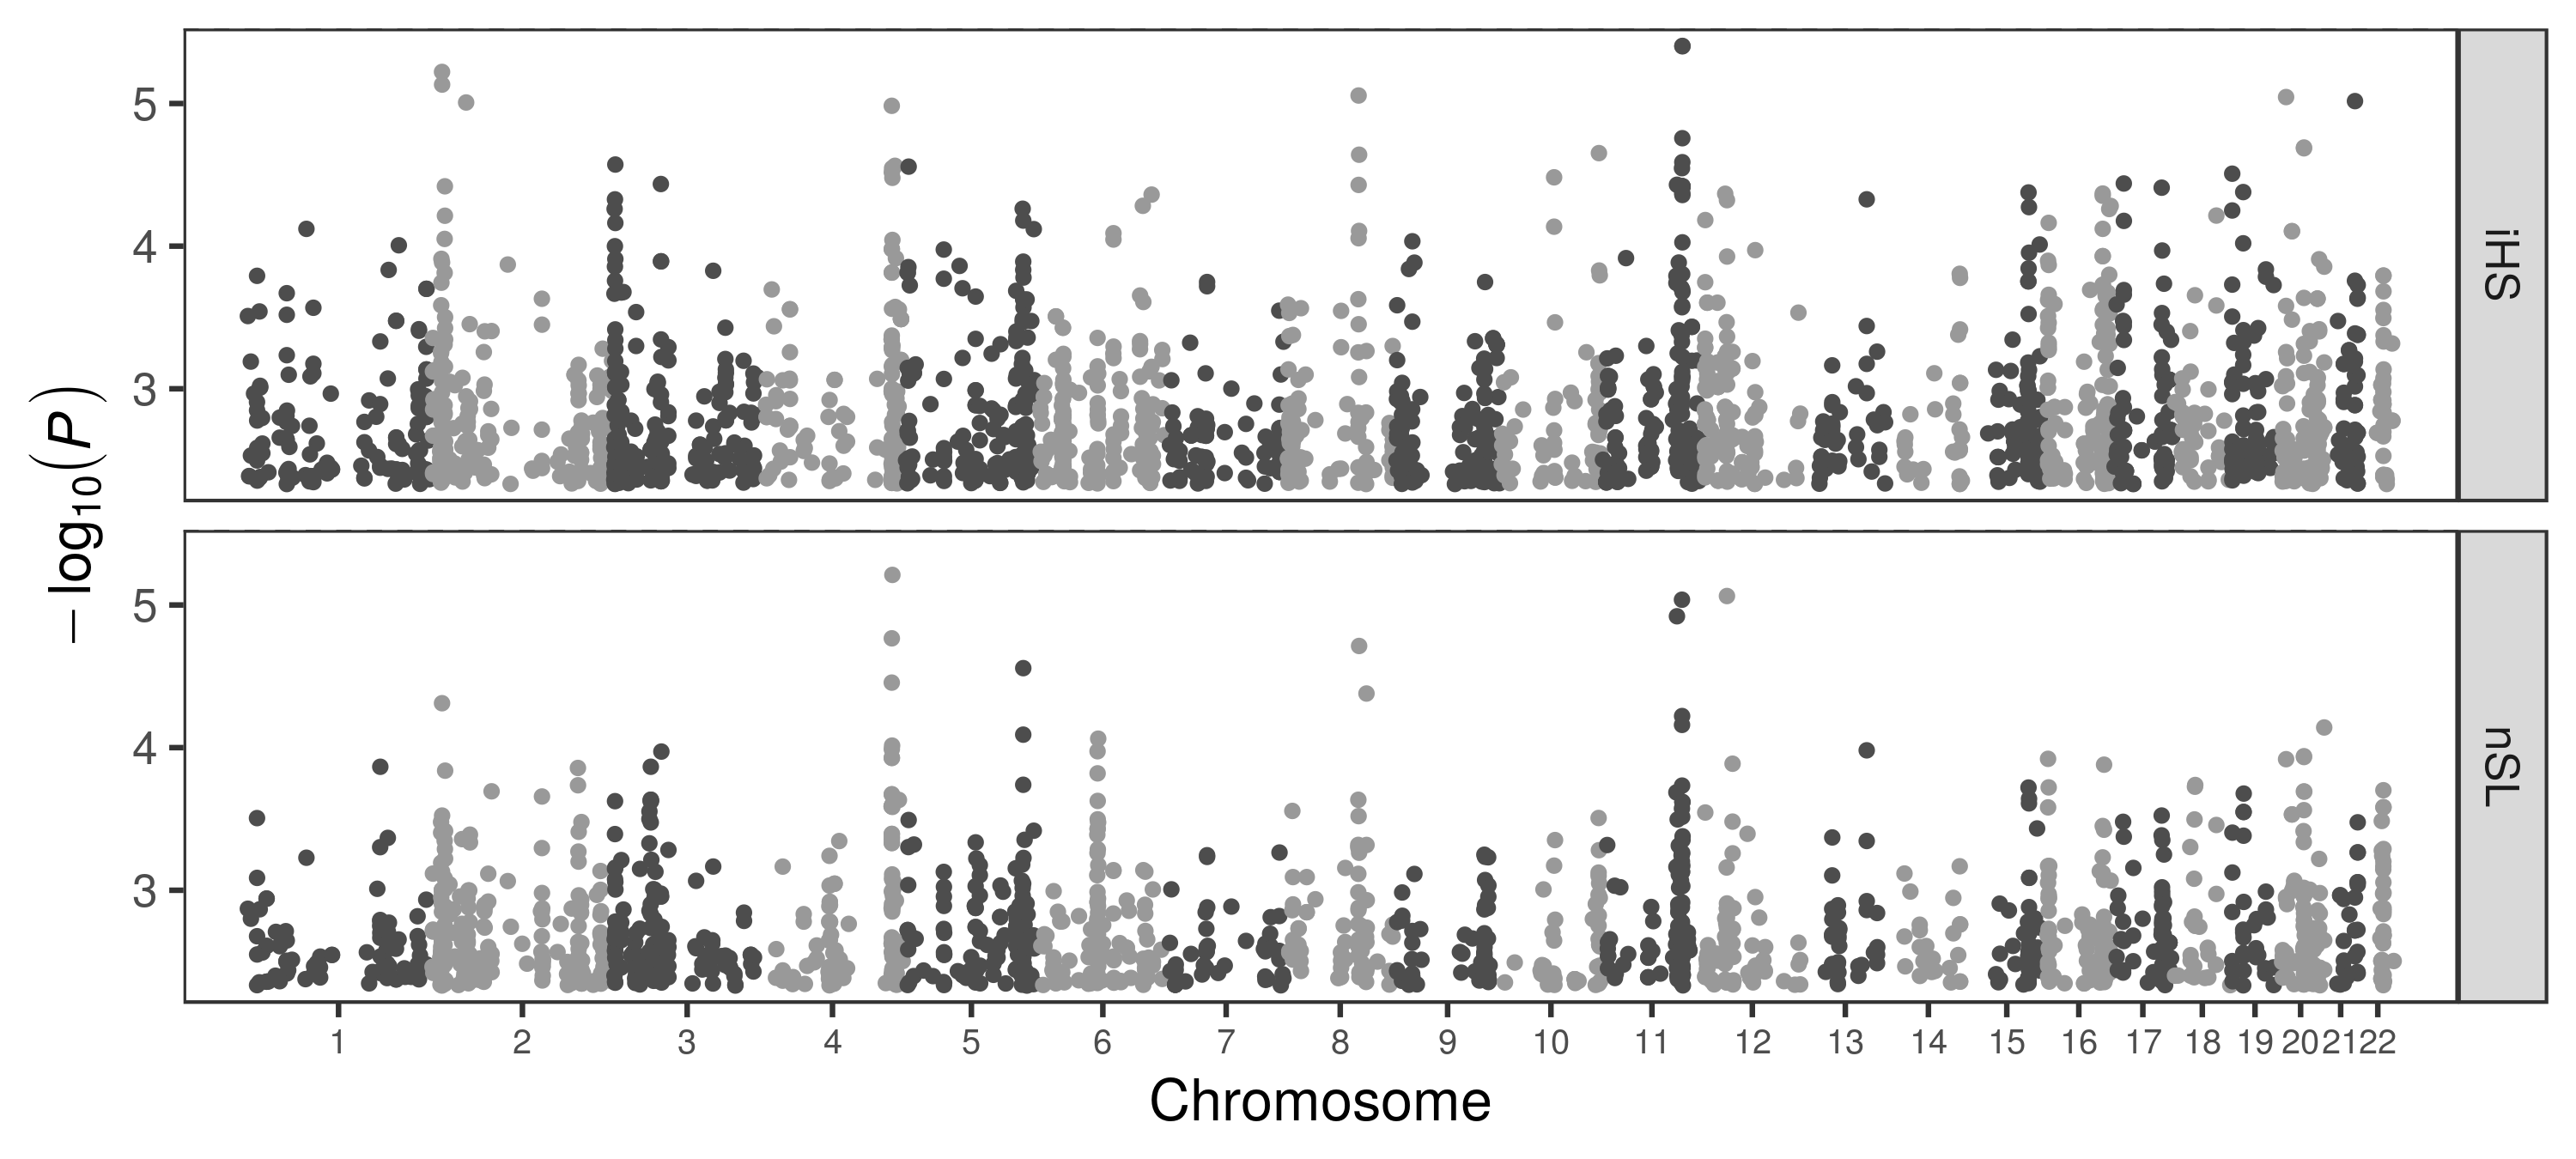
\includegraphics[height=0.4\textheight,angle=90]{images/03_selectionpipeline/cimHapMan} 

}

\caption[Manhattan plot for significant markers in \acrlong{cim} for both \acrshort{ihs} and \acrshort{nsl}.]{Manhattan plot for significant markers in \gls{cim} for
both \gls{ihs} and \gls{nsl}.}\label{fig:cimHapMan}
\end{figure}

\subsubsection{\texorpdfstring{New Zealand M\tex{\={a}}ori genome-wide
selection
analysis}{New Zealand Mori genome-wide selection analysis}}\label{new-zealand-mori-genome-wide-selection-analysis}

\paragraph{Pathway enrichment analysis of genome-wide selected loci in
NZM}\label{nzmPath}

The pathway gene-set enrichment analysis from Enrichr on the KEGG 2016
pathways had 32 pathways that were significant after multiple testing
correction, this was the largest number of pathways out of the
Polynesian populations (Table \ref{tab:keggPath}). On average only 9.3\%
of a pathway was represented by the genes. Thirty-one pathways were from
the significant genes for \gls{nsl}, with many in common with \gls{cim}.
Calcium transporters and voltage gated calcium channels featured in many
pathways that were in common. Compared to the \gls{cim} pathway results,
there were more hormone-based pathways that were significant, such as
renin secretion, oxytocin signalling pathway, adrenergic signalling in
cardiomyocytes, thyroid hormone synthesis, aldosterone synthesis and
secretion, insulin secretion, and GnRH signalling pathway. Furthermore,
diabetes-related pathways were significant such as type 2 diabetes
mellitus, insulin secretion, and pancreatic secretion pathways. The
genes that were shared in the most pathways included two adenlyate
cylases (\emph{ADCY8} and \emph{ADCY9}), two phospholipase C genes
(\emph{PLCB1} and \emph{PLCB4}), and calcium voltage-gated channel
subunits (\emph{CACNA1C} and \emph{CACNA1D}). Similar to \gls{cim},
there was a single pathway that was significant from the \gls{td} list
and that too was for bacterial invasion of epithelial cells.

\paragraph{\texorpdfstring{Selection from haplotypic statistics in
\gls{nzm} -
genome-wide}{Selection from haplotypic statistics in  - genome-wide}}\label{selection-from-haplotypic-statistics-in---genome-wide}

The significant markers from \gls{ihs} and \gls{nsl} were converted to
P-values and plotted on a Manhattan plot (Figure \ref{fig:nzmHapMan}).
The most extreme markers for \gls{ihs} (by position,
-log\textsubscript{10}(P) \textgreater{} 4.8) were: chr2 - rs2710684;
chr3 - rs74823804 and rs2280162; chr8 - rs11987519; chr9 - rs2780246;
chr10 - rs4075326 and rs11017145; chr16 - rs28564718 and rs3743759. For
\gls{nsl}, the markers were: chr4 - rs1491411; chr8 - rs11987519; chr12
- rs7977414. From the haplotypic tests for selection (\gls{ihs} and
\gls{nsl}) there were 122 genes that were only significant in \gls{nzm}
for \gls{ihs}, and 93 for \gls{nsl}. Looking at the genes represented by
the most extreme 100 \gls{ihs} and \gls{nsl} markers there were 30 genes
for \gls{ihs}, and 40 genes for \gls{nsl}. There were 12 genes in common
between the two sets (\emph{CTNNA3}, \emph{WWOX}, \emph{KCNS3},
\emph{NRXN1}, \emph{ADAM29}, \emph{VSNL1}, \emph{BCCIP}, \emph{BICD1},
\emph{DHX32}, \emph{SLC35F2}, \emph{STAU2}, and \emph{TENM3}).
\emph{CTNNA3} had five markers in the top 100 for \gls{nsl} (rs2441727,
rs12220315, rs1911341, rs2660024, and rs10997250), and was also the gene
for \gls{nzm} that had the most overall significant markers for both
\gls{ihs} and \gls{nsl}. There were 40 genes that had at least 20
populations with significant markers for \gls{xpehh} in only NZM from
the Polynesian populations, only one (\emph{PAX5}) of which was
associated with obesity \citep{melka2012genome}. There were eight genes,
\emph{LYST}, \emph{PHIP}, \emph{CTNNA3}, \emph{RAD51AP2}, \emph{SUPT3H},
\emph{EPB41L4A}, \emph{RAD51B}, and \emph{VSNL1}, that had at least one
significant marker for \gls{ihs} or \gls{nsl}, and also had a window in
the 1\textsuperscript{st} percentile from three or more statistics from
\gls{td}, \gls{fwh}, \gls{flf}, and \gls{ze}.




\begin{figure}

{\centering 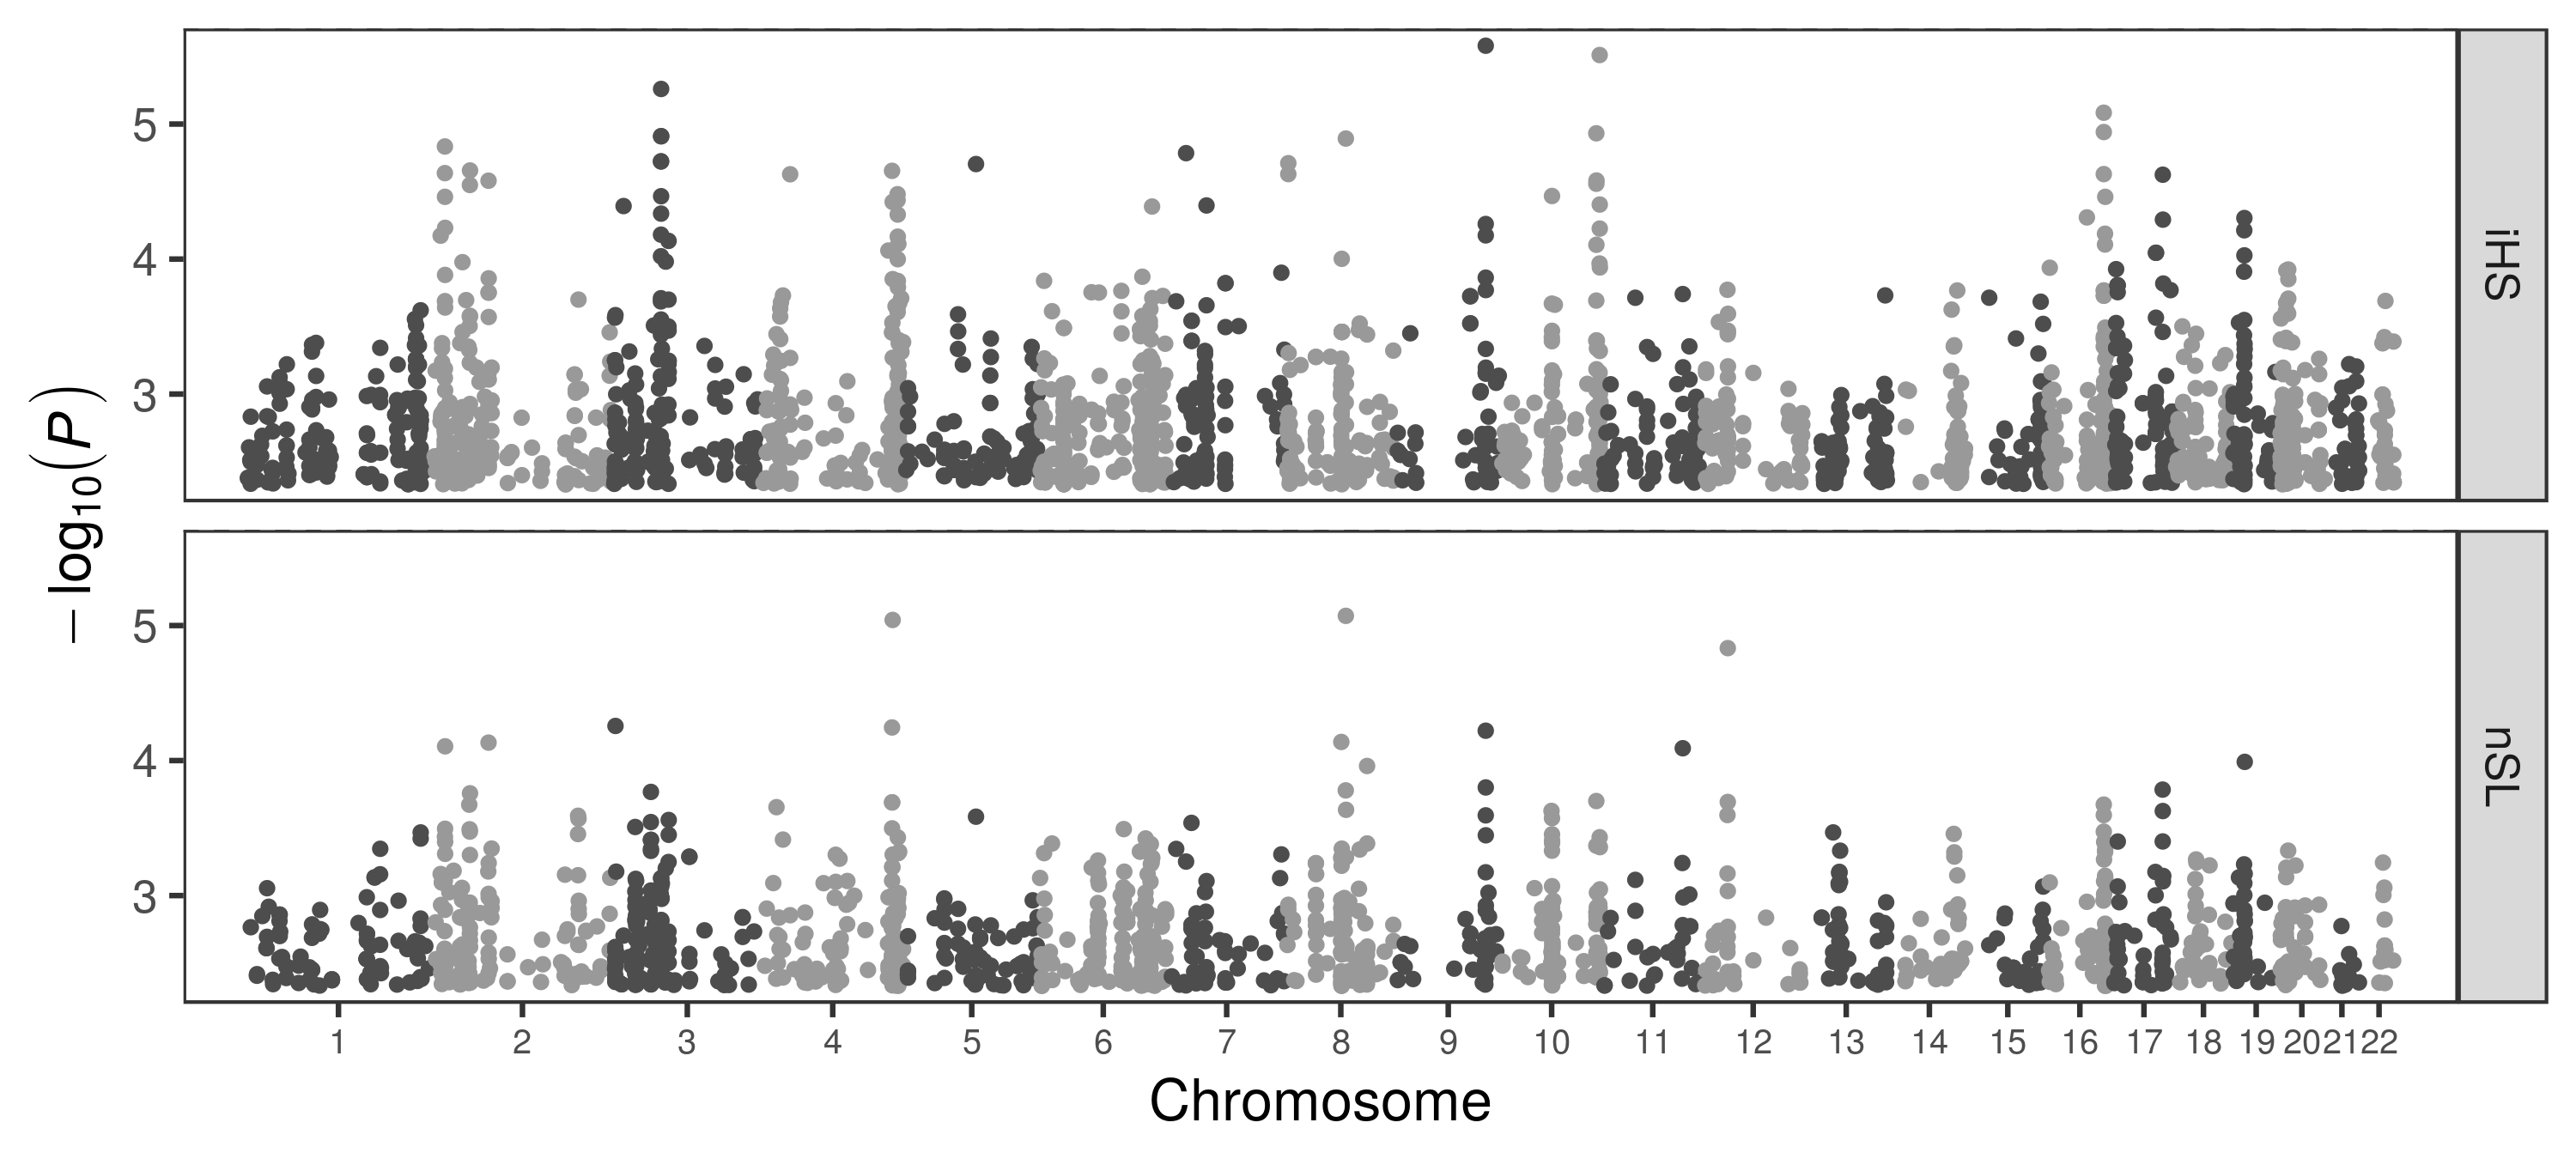
\includegraphics[height=0.4\textheight,angle=90]{images/03_selectionpipeline/nzmHapMan} 

}

\caption[Manhattan plot for significant markers in \acrlong{nzm} for both \acrshort{ihs} and \acrshort{nsl}.]{Manhattan plot for significant markers in \gls{nzm} for
both \gls{ihs} and \gls{nsl}.}\label{fig:nzmHapMan}
\end{figure}

\paragraph{\texorpdfstring{Contiguous regions of score depression in
\gls{nzm}}{Contiguous regions of score depression in }}\label{contiguous-regions-of-score-depression-in-1}

The regions of contiguous depressed score from the 1\textsuperscript{st}
percentile of windows that also contained markers with a significant
\gls{ihs} or \gls{nsl} value covered three regions of the genome for
\gls{nzm}. Two of the regions were for \gls{td}, the first was 270kb at
chr2:24215002-24485001, and overlapped the region in \gls{cim}. It had a
single significant marker for \gls{ihs} in each of
\emph{MFSD2B}/\emph{FKBP1B} (rs10185680), and \emph{FAM228B}
(rs10197527). The second \gls{td} region was 260 kb at
chr4:106555002-106815001 and had a single significant marker for
\gls{nsl} in \emph{INTS12} (rs2553453). A 200 kb region for \gls{flf} at
chr2:179395002-179595001 had four significant markers in \emph{TTN-AS1}
for \gls{ihs} (rs3731752, rs2278196, rs72648270, and rs3813243).

No contiguous regions of score depression intersected with genes
associated with urate, kidney disease, or \gls{t2d}. There were 2
regions that intersected obesity-associated loci; for \gls{td} a 320 kb
region at chr16:67145002-67465001 contained \emph{KCTD19}, and for
\gls{flf}, 220 kb at chr16:3555002-3775001 contained \emph{NLRC3}.
\emph{EDC4} which is associated with metabolic syndrome
\citep{kristiansson2012genome}, had slightly differing regions that
covered it. \Gls{td} was 330 kb spanning chr16:67775002-68105001, and
\gls{flf} was 320 kb spanning chr16:67775002-68095001.

\subsubsection{Samoan genome-wide selection
analysis}\label{samoan-genome-wide-selection-analysis}

\paragraph{Pathway enrichment analysis of genome-wide selected loci in
SAM}\label{samPath}

Only two pathways were significant for the gene-set pathway enrichment
analysis using Enrichr (Table \ref{tab:keggPath}). The pathway term
``ABC transporters'' was significant for gene list from \gls{ihs}
(adjusted P = 0.0128) with 9 of 44 genes. The genes were \emph{ABCC4},
\emph{ABCA5}, \emph{ABCC8}, \emph{ABCC5}, \emph{ABCB5}, \emph{TAP2},
\emph{ABCA9}, \emph{ABCB8}, and \emph{ABCA8}. The second pathway that
was significant was ``long-term potentiation'' and that was from the
\gls{nsl} gene list (adjusted P = 0.0213) with 9 of 66 genes. The genes
were \emph{PPP3CA}, \emph{GNAQ}, \emph{RPS6KA1}, \emph{PRKCA},
\emph{CACNA1C}, \emph{PLCB1}, \emph{PLCB2}, \emph{CAMK2G}, and
\emph{RAPGEF3}.

\paragraph{\texorpdfstring{Selection from haplotypic statistics in
\gls{sam} -
genome-wide}{Selection from haplotypic statistics in  - genome-wide}}\label{selection-from-haplotypic-statistics-in---genome-wide-1}

The significant markers for \gls{ihs} and \gls{nsl} are shown by
position across the genome as a Manhattan plot after conversion to
P-values in Figure \ref{fig:samHapMan}. The most extreme markers for
\gls{ihs} (by position, -log\textsubscript{10}(P)) were: chr1 -
rs10495181; chr4 - rs12331849; chr11 - rs6578634; chr13 - rs4941616;
chr16 - rs12596728. For \gls{nsl} they were: chr17 - rs11654176 and
rs1860316. From the haplotypic tests for selection (\gls{ihs} and
\gls{nsl}) there were 110 genes that were only significant in \gls{sam}
for \gls{ihs}, and 90 for \gls{nsl}. The genes with the most significant
markers for \gls{ihs} were \emph{CDH23} and \emph{CNTN5} with 12
significant markers each. The gene with the most significant markers for
\gls{nsl} was \emph{CDH23} with 16 markers. Looking at the most extreme
100 markers for \gls{nsl} there were 35 genes represented, \emph{SNX29}
had the most with three markers (rs350277, rs7201595, and rs12931604).
For \gls{ihs}, the gene with the most markers in the most extreme 100
was \emph{C11orf65}, with three (rs425538, rs7931930, and rs11212617).
There was a total of 39 genes represented. Between the top markers for
both \gls{ihs} and \gls{nsl} there were 10 genes that were in common
(\emph{SNX29}, \emph{LINC00693}, \emph{BANK1}, \emph{DLC1},
\emph{DUSP13}, \emph{HBE1}, \emph{HBG2}, \emph{MYCBP2}, \emph{NLRP1},
and \emph{SAMD8}).

There were ten genes that had windows from at least three of the
frequency-based statistics and also had at least a single significant
marker for either \gls{ihs} or \gls{nsl}. The genes were \emph{DISP1}
(\gls{ihs}: rs2789931 and rs2789954), \emph{PARD3B} (\gls{ihs} and
\gls{nsl}: rs13000345), \emph{C4orf45} (\gls{ihs} and \gls{nsl}:
rs11722868), \emph{NEK1} (\gls{ihs}: rs4235024), \emph{CNTNAP2}
(\gls{ihs}: rs2620441, rs2249958, and rs17170777; \gls{nsl}: rs2249958,
rs17170777, and rs10255956), \emph{CTNNA3} (\gls{ihs}: rs1948946;
\gls{nsl} rs4297361, rs1948946, rs2764813, rs2394324, and rs10823054),
\emph{CEP112} (\gls{ihs}: rs11652795; \gls{nsl} rs1373074),
\emph{CNTNAP5} (\gls{nsl}: rs314710 and rs2602647), \emph{SUPT3H}
(\gls{nsl}: rs9472376), and \emph{DGKI} (\gls{nsl}: rs12056089).
\Gls{xpehh} had 19 genes that had at least 20 populations with
significant markers in only \gls{sam} from the Polynesian populations
but none had been associated with urate or related co-morbidities.




\begin{figure}

{\centering 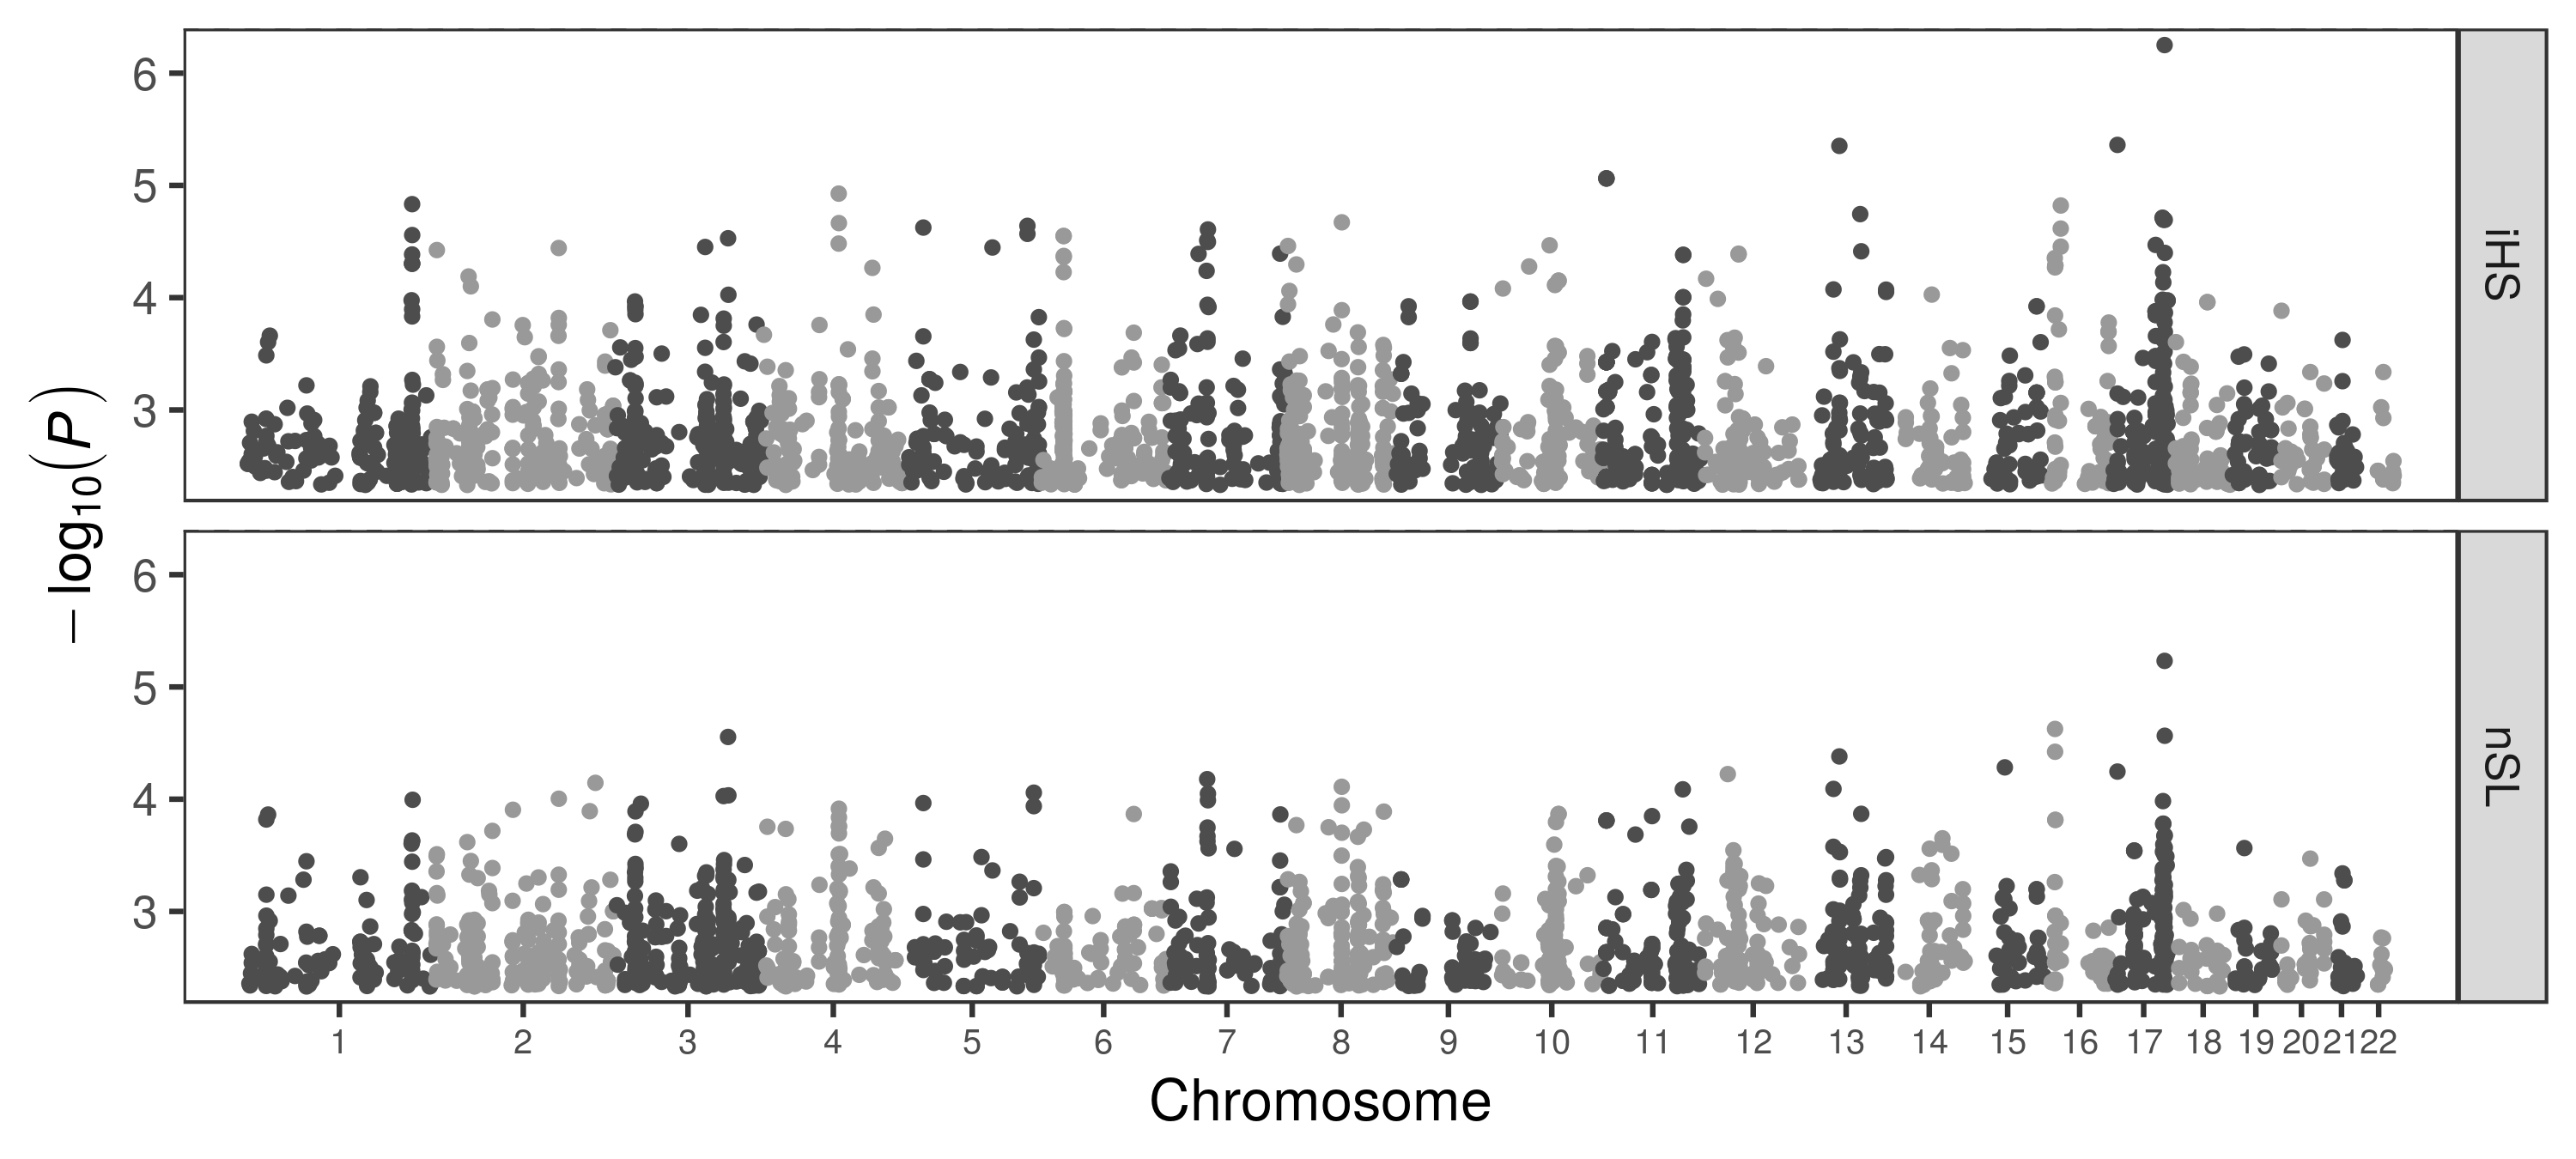
\includegraphics[height=0.4\textheight,angle=90]{images/03_selectionpipeline/samHapMan} 

}

\caption[Manhattan plot for significant markers in \acrlong{sam} for both \acrshort{ihs} and \acrshort{nsl}.]{Manhattan plot for significant markers in \gls{sam} for
both \gls{ihs} and \gls{nsl}.}\label{fig:samHapMan}
\end{figure}

\paragraph{\texorpdfstring{Contiguous regions of score depression in
\gls{sam}}{Contiguous regions of score depression in }}\label{contiguous-regions-of-score-depression-in-2}

There were no contiguous depressed score regions that intersected with
genes associated with urate, obesity, \gls{t2d}, kidney disease, or
metabolic syndrome. Regions of contiguously depressed score that also
had significant markers for \gls{ihs} or \gls{nsl} in \gls{sam} covered
three regions of the genome across two statistics. \Gls{td} had two
regions, the first was 400 kb at chr4:170025002-170425001 and had a
single significant marker for \gls{ihs} (rs4235024) nearby in
\emph{NEK1}. The second region was 300 kb in length and was found at
chr10:76685002-76985001. It had significant markers in \emph{KAT6B}
(\gls{ihs} and \gls{nsl}:rs3213967), and in \emph{SAMD8/DUSP13}
(\gls{ihs} and \gls{nsl}: rs7912300 and rs10824274). \Gls{flf} had a
single 200 kb region at chr1:26465002-26665001 that had a single
significant marker for \gls{nsl} in \emph{CNKSR1} (rs2783633), and two
markers for \gls{ihs} and three for \gls{nsl} in \emph{AIM1L} (\gls{ihs}
and \gls{nsl}:rs11247916 and rs10751735; \gls{nsl}: rs4659431).

\subsubsection{Tongan genome-wide selection
analysis}\label{tongan-genome-wide-selection-analysis}

\paragraph{Pathway enrichment analysis of genome-wide selected loci in
TON}\label{tonPath}

Pathway enrichment analysis from the Enrichr KEGG 2016 pathways produced
11 different pathways that were significant after multiple testing
correction (Table \ref{tab:keggPath}). Of the \gls{sfs} based methods,
only \gls{flf} had a significant pathway and this was ``Olfactory
transduction''. There were two pathway terms that were significant from
the \gls{ihs} results, these were ``ABC transporters'' and
``ECM-receptor interaction''. These were also significant in the
\gls{nsl} results, along with another eight terms (Table
\ref{tab:keggPath}). The genes that were included in the ``ABC
transporters'' pathway from the significant markers of both \gls{ihs}
and \gls{nsl} were: \emph{ABCC8}, \emph{TAP2}, \emph{ABCA9},
\emph{ABCA8}, and \emph{ABCG2}. From only \gls{ihs} markers \emph{ABCA5}
\emph{ABCA6}, \emph{ABCC5}, \emph{ABCB} were included, and from only
\gls{nsl} markers, \emph{ABCB8} was included. Genes with significant
markers for both \gls{ihs} and \gls{nsl} in the ``ECM-receptor
interaction'' pathway included \emph{COL4A2}, \emph{ITGB5},
\emph{ITGA1}, \emph{ITGA2}, \emph{SPP1} and \emph{ITGB6}. From only
\gls{ihs} markers \emph{LAMA5}, \emph{TNXB}, \emph{TNC}, \emph{COL6A3},
and \emph{HMMR} were included, and from only \gls{nsl} makers,
\emph{COL4A1}, and \emph{ITGA9} were included. Five of the significant
pathway terms were only significant in \gls{ton} out of the Polynesian
populations.

\paragraph{\texorpdfstring{Selection from haplotypic statistics in
\gls{ton} -
genome-wide}{Selection from haplotypic statistics in  - genome-wide}}\label{selection-from-haplotypic-statistics-in---genome-wide-2}

The significant markers for \gls{ihs} and \gls{nsl} were plotted
genome-wide after conversion to P-values in a Manhattan plot (Figure
\ref{fig:tonHapMan}). The most extreme \gls{ihs} markers (by position,
-log\textsubscript{10}(P)) were: chr1 - rs12042853, rs10495181,
rs4240931, and rs2800853; chr7 - rs10485976, rs6962297, rs296307,
rs6969276, rs7791859, and rs1405425; chr8 - rs4349972; chr10 - rs7097067
and rs7923688; chr11 - rs6578634; chr13 - rs4941616; chr16 rs154148 and
rs350277; chr17 - rs6504539, rs1860316 and rs16976276. For \gls{nsl}
they were: chr7 - rs7791859 and rs1405425; chr8 - rs2605867; chr13 -
rs4941616; chr16 - rs350277. In total there were 105 genes that were
only significant in \gls{ton} for \gls{ihs}, and 108 for \gls{nsl}. In
the most extreme 100 \gls{nsl} marker scores, there were 32 genes
represented with \emph{SNX29} having three markers (rs350277, rs7201595,
and rs12931604), and \emph{CDH23} having two (rs2394801 and rs10762462)
from the 100. The most extreme 100 marker scores for \gls{ihs} had 30
genes represented with \emph{SNX29} having five markers (rs350277,
rs7201595, rs7198595, rs7189759, and rs12931604), \emph{PCDH15} having
three (rs4272709, rs11004106, and rs4935502), and \emph{DNAH11} having
two (rs10485976 and rs1989904) of the 100. There was an overlap between
the two gene lists for the most extreme 100 of six genes, with
\emph{SNX29}, and \emph{DNAH11} having the largest number of extreme
markers for both \gls{ihs}, and \gls{nsl}. The genes with the largest
number of significant markers overall for \gls{ihs} and \gls{nsl} were
\emph{CPNE4} (16 markers for both \gls{ihs} and \gls{nsl}), \emph{SNX29}
(15 markers for \gls{ihs} and 16 for \gls{nsl}), \emph{CDH23} (11
markers for \gls{ihs} and 12 for \gls{nsl}), \emph{PCDH15} (12 markers
for \gls{nsl}), and \emph{BANK1} (9 markers for \gls{ihs} and 10 for
\gls{nsl}). There were 37 genes that had at least 20 populations with
significant markers for \gls{xpehh} in only TON from the Polynesian
populations, including \emph{IGF1R}, \emph{JAZF1}, and \emph{PEPD} which
had been associated with urate or co-morbidities.

There were seven genes that had at least one significant marker for
either \gls{ihs} or \gls{nsl}, and windows in the 1\textsuperscript{st}
percentile for at least three frequency-based intra-population selection
and neutrality statistics. They were \emph{C4orf45}, \emph{SUPT3H},
\emph{CTNNA3}, \emph{SAMD8}, \emph{EXT2}, \emph{LPO}, and \emph{NRXN3.}




\begin{figure}

{\centering 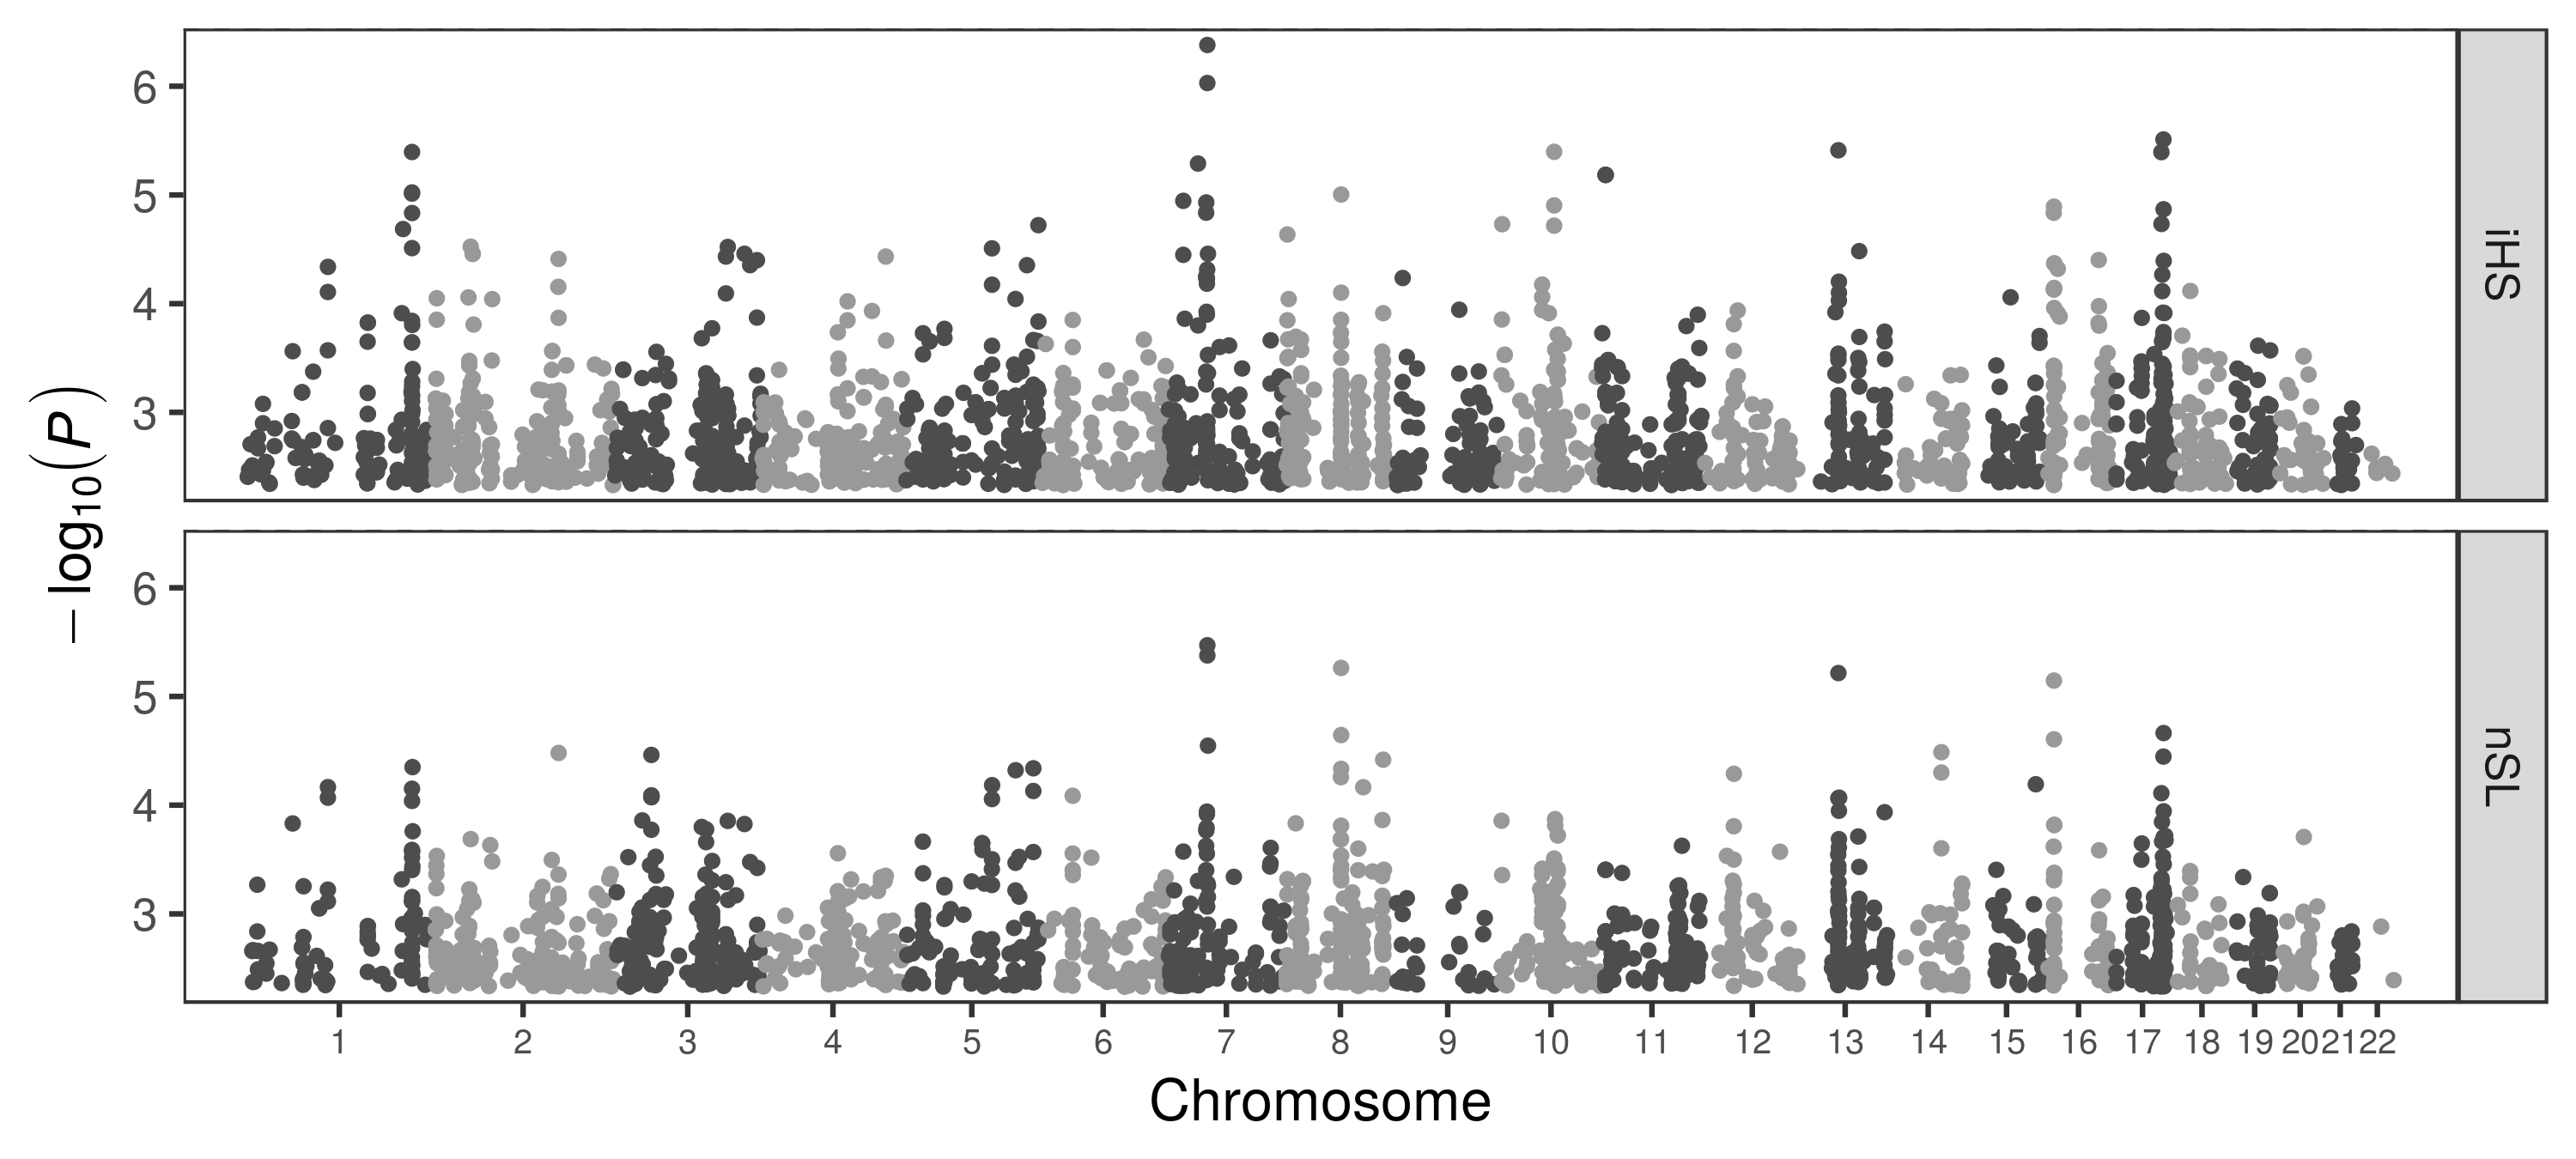
\includegraphics[height=0.4\textheight,angle=90]{images/03_selectionpipeline/tonHapMan} 

}

\caption[Manhattan plot for significant markers in \acrlong{ton} for both \acrshort{ihs} and \acrshort{nsl}.]{Manhattan plot for significant markers in \gls{ton} for
both \gls{ihs} and \gls{nsl}.}\label{fig:tonHapMan}
\end{figure}

\paragraph{\texorpdfstring{Contiguous regions of score depression in
\gls{ton}}{Contiguous regions of score depression in }}\label{contiguous-regions-of-score-depression-in-3}

There were no contiguous depressed score regions that intersected genes
associated with urate, \gls{t2d}, kidney disease, or metabolic syndrome.
There was one region that intersected the obesity associated gene
\emph{CCR3} for \gls{td} and was 260 kb in length at
chr3:46035002-46295001. There were three regions with contiguous
depressed score that also had significant markers for \gls{ihs} or
\gls{nsl} in \gls{ton}. \Gls{td} had two regions. The first similar to
\gls{sam}, was at chr10:76685002-76985001 and spanned 300 kb and had
significant markers in \emph{KAT6B} (\gls{ihs} and \gls{nsl}:rs1551067
and rs3213967), \emph{SAMD8} (\gls{ihs} and \gls{nsl}: rs10509355,
rs10824274, and rs7912300), and in \emph{DUSP13} (\gls{ihs} and
\gls{nsl}: rs10824274 and rs7912300). The second region at
chr17:56125002-56415001 was 290 kb and had a single significant marker
(rs9892223) for \gls{ihs} in both \emph{EPX} and \emph{LPO}. \Gls{flf}
had a slightly shifted region that also intersected \emph{EPX} and
\emph{LPO} and had the same significant markers as the \gls{td} region,
but also included \emph{RNF43/BZRAP1-AS1} - which also had a single
significant marker for \gls{ihs} (rs2257205). The region was at
chr17:56205002-56455001 and was 250 kb in length.

\subsection{Selection in disease-associated
genes}\label{selection-in-disease-associated-genes}

\subsubsection{Selection in Polynesian populations for genes associated
with urate and metabolic
disease}\label{selection-in-polynesian-populations-for-genes-associated-with-urate-and-metabolic-disease}

In order to establish if there was evidence of selection in genes
associated with urate and diseases with hyperuricaemia as a
co-morbidity, loci that associated with these conditions were extracted
from the \gls{gwas} catalog (as per section \ref{diseaselist}, see Table
\ref{tab:gwascatref} for references for each trait) and neutrality and
selection statistics that intersected these loci were collated. Table
\ref{tab:superDiseaseGenesTab} shows the breakdown of the number of
different statistics by population that met the significance thresholds
for the \gls{sfs} based statistics, the haplotype based statistics, and
the overlap between the frequency spectrum and haplotypic methods. The
\gls{cim} population had the least number of genes of the Polynesian
populations that had a significant result out of the genes that were
associated with urate. The Polynesian populations had the fewest number
of genes with significant \gls{ihs} or \gls{nsl} for obesity and the
Western Polynesian populations had the fewest number of genes for
\gls{t2d}.

Figure \ref{fig:intraSelGenes} shows the genes associated with urate,
gout and related diseases that had a significant marker with either
\gls{ihs} or \gls{nsl} and also had a significant window from a
\gls{sfs}-based statistic in at least one Polynesian population. There
were only 10 genes that met this criteria, of which, the \gls{t2d}
associated gene, \emph{PTPRD}, was the only gene that met the criteria,
and also had significant markers from all Polynesian populations in
\gls{ihs}. The obesity-associated genes \emph{GRID1}, \emph{FHIT}, and
\emph{ERBB4}, all had windows from \gls{fwh} that were significant in
all Polynesian populations. \emph{ERBB4} also had significant windows
for all Polynesian populations for \gls{td}.








\begin{figure}
\includegraphics{_bookdown_files/03-SelectionPipeline_files/figure-latex/intraSelGenes-1} \caption[Genes associated with urate, gout, obesity, type 2 diabetes, kidney disease, and metabolic syndrome with evidence from site-frequency spectrum and haplotypic statistics in Polynesian populations.]{Genes associated with urate, gout, obesity,
\gls{t2d}, kidney disease, and metabolic syndrome having both
significance in intra-population \gls{sfs} and haplotypic based methods
in at least one Polynesian population. Numbers inside boxes indicate the
number of significant windows (\gls{sfs} methods) or \glspl{snp}
(haplotypic methods) for the population.}\label{fig:intraSelGenes}
\end{figure}

\begin{table}[!h]

\caption[Number of genes with evidence of possible positive selection in super populations from intra-population tests from urate and co-morbidities \acrshort{gwas} associated loci.]{\label{tab:unnamed-chunk-50}\label{tab:superDiseaseGenesTab} Number of genes with evidence of possible positive selection in super populations from intra-population tests from urate and co-morbidities \gls{gwas} associated loci.}
\centering
\begin{threeparttable}
\begin{tabular}[t]{llrrrrrrrrrrrrrrr}
\toprule
\multicolumn{1}{c}{} & \multicolumn{1}{c}{} & \multicolumn{3}{c}{Urate / Gout} & \multicolumn{3}{c}{Obesity} & \multicolumn{3}{c}{T2D} & \multicolumn{3}{c}{Kidney Disease} & \multicolumn{3}{c}{Metabolic Syndrome} \\
\cmidrule(l{2pt}r{2pt}){3-5} \cmidrule(l{2pt}r{2pt}){6-8} \cmidrule(l{2pt}r{2pt}){9-11} \cmidrule(l{2pt}r{2pt}){12-14} \cmidrule(l{2pt}r{2pt}){15-17}
\rotatebox{90}{Population} & \rotatebox{90}{Super Pop.} & \rotatebox{90}{SFS} & \rotatebox{90}{Hap.} & \rotatebox{90}{Com.} & \rotatebox{90}{SFS} & \rotatebox{90}{Hap.} & \rotatebox{90}{Com.} & \rotatebox{90}{SFS} & \rotatebox{90}{Hap.} & \rotatebox{90}{Com.} & \rotatebox{90}{SFS} & \rotatebox{90}{Hap.} & \rotatebox{90}{Com.} & \rotatebox{90}{SFS} & \rotatebox{90}{Hap.} & \rotatebox{90}{Com.}\\
\midrule
ACB & AFR & 9 & 9 & 0 & 34 & 46 & 14 & 9 & 18 & 2 & 5 & 5 & 0 & 2 & 0 & 0\\
ASW & AFR & 8 & 5 & 1 & 31 & 44 & 11 & 8 & 21 & 3 & 10 & 7 & 2 & 4 & 3 & 1\\
ESN & AFR & 8 & 4 & 0 & 29 & 44 & 7 & 9 & 18 & 3 & 7 & 6 & 1 & 3 & 2 & 0\\
GWD & AFR & 5 & 4 & 0 & 41 & 43 & 8 & 9 & 15 & 3 & 6 & 6 & 1 & 4 & 3 & 0\\
LWK & AFR & 5 & 7 & 0 & 30 & 46 & 5 & 8 & 16 & 3 & 5 & 7 & 1 & 3 & 3 & 0\\
MSL & AFR & 7 & 10 & 1 & 35 & 38 & 10 & 10 & 11 & 3 & 6 & 10 & 2 & 2 & 3 & 1\\
YRI & AFR & 7 & 5 & 0 & 35 & 40 & 9 & 10 & 13 & 4 & 6 & 7 & 1 & 1 & 0 & 0\\
CLM & AMR & 10 & 4 & 1 & 30 & 36 & 6 & 8 & 15 & 1 & 8 & 3 & 0 & 2 & 5 & 1\\
MXL & AMR & 9 & 2 & 0 & 30 & 35 & 5 & 8 & 14 & 0 & 10 & 1 & 0 & 4 & 4 & 1\\
PEL & AMR & 10 & 3 & 0 & 29 & 29 & 6 & 11 & 18 & 3 & 6 & 2 & 0 & 2 & 2 & 0\\
PUR & AMR & 7 & 7 & 1 & 37 & 43 & 11 & 9 & 11 & 2 & 6 & 6 & 1 & 3 & 4 & 1\\
CDX & EAS & 4 & 2 & 0 & 21 & 37 & 6 & 11 & 11 & 3 & 5 & 3 & 1 & 1 & 2 & 0\\
CHB & EAS & 4 & 2 & 0 & 25 & 28 & 5 & 14 & 11 & 2 & 4 & 3 & 0 & 1 & 0 & 0\\
CHS & EAS & 7 & 2 & 0 & 22 & 33 & 6 & 10 & 10 & 2 & 5 & 2 & 0 & 1 & 1 & 0\\
JPT & EAS & 7 & 2 & 0 & 25 & 36 & 5 & 7 & 12 & 1 & 5 & 1 & 0 & 1 & 1 & 0\\
KHV & EAS & 2 & 3 & 0 & 25 & 34 & 9 & 6 & 11 & 2 & 6 & 1 & 0 & 1 & 1 & 0\\
CEU & EUR & 13 & 3 & 1 & 31 & 31 & 8 & 8 & 13 & 0 & 7 & 4 & 1 & 2 & 4 & 0\\
FIN & EUR & 5 & 3 & 1 & 27 & 35 & 5 & 6 & 14 & 0 & 5 & 4 & 1 & 1 & 3 & 0\\
GBR & EUR & 10 & 4 & 1 & 32 & 35 & 9 & 10 & 16 & 3 & 7 & 3 & 1 & 1 & 3 & 0\\
IBS & EUR & 9 & 3 & 0 & 34 & 38 & 9 & 8 & 12 & 1 & 7 & 2 & 1 & 1 & 4 & 0\\
NZC & EUR & 13 & 6 & 2 & 27 & 34 & 7 & 9 & 17 & 2 & 10 & 3 & 1 & 2 & 4 & 0\\
TSI & EUR & 13 & 4 & 1 & 27 & 35 & 11 & 6 & 14 & 2 & 6 & 1 & 0 & 2 & 7 & 1\\
CIM & POL & 5 & 1 & 0 & 29 & 17 & 2 & 11 & 9 & 2 & 5 & 0 & 0 & 1 & 0 & 0\\
NZM & POL & 8 & 1 & 0 & 31 & 21 & 5 & 13 & 10 & 2 & 4 & 1 & 0 & 2 & 3 & 0\\
SAM & POL & 5 & 4 & 0 & 27 & 20 & 4 & 14 & 4 & 0 & 7 & 3 & 0 & 1 & 1 & 0\\
TON & POL & 8 & 5 & 0 & 22 & 25 & 4 & 14 & 7 & 1 & 7 & 3 & 0 & 3 & 2 & 0\\
BEB & SAS & 7 & 3 & 0 & 25 & 25 & 5 & 7 & 13 & 2 & 10 & 4 & 1 & 0 & 5 & 0\\
GIH & SAS & 4 & 1 & 0 & 24 & 23 & 6 & 8 & 14 & 3 & 4 & 1 & 0 & 0 & 3 & 0\\
ITU & SAS & 6 & 3 & 0 & 20 & 24 & 5 & 6 & 14 & 2 & 8 & 2 & 1 & 1 & 4 & 0\\
PJL & SAS & 7 & 2 & 1 & 21 & 30 & 3 & 7 & 16 & 3 & 7 & 1 & 0 & 0 & 3 & 0\\
STU & SAS & 10 & 0 & 0 & 26 & 28 & 8 & 6 & 12 & 2 & 6 & 3 & 1 & 2 & 3 & 0\\
\bottomrule
\end{tabular}
\begin{tablenotes}
\item Hap = haplotypic. Com = combined. Combined is the number of genes that had both SFS and haplotypic evidence.
\end{tablenotes}
\end{threeparttable}
\end{table}

\FloatBarrier

\paragraph{Selection in Polynesian populations for genes associated with
urate and
gout}\label{selection-in-polynesian-populations-for-genes-associated-with-urate-and-gout}

The 62 loci identified in the \gls{gwas} catalog (see Table
\ref{tab:gwascatref} for references) as being associated with urate and
gout only had a small proportion with any evidence of possible
selection, 18 in Polynesian populations. In the Polynesian populations,
from the intra-population neutrality and selection statistics, there
were 18 genes that had some evidence. However, there were only nine
genes with haplotypic evidence, and only one gene (\emph{RREB1}) that
had both haplotypic and \gls{sfs}-based evidence. Overall, the
Polynesian populations did not have more urate genes with evidence for
selection than the other populations (Table
\ref{tab:superDiseaseGenesTab}).

The two main effect loci for serum urate, \emph{SLC2A9} and \emph{ABCG2}
both had limited evidence of selection. \emph{SLC2A9} did not have any
values for \gls{ihs} or \gls{nsl} because of an extended region of no
recombination leading to a large gap in the reference genome which
caused the \gls{ehh} calculation to be terminated. There was evidence
with \gls{flf} which had windows from \emph{SLC2A9} in the
1\textsuperscript{st} percentile from \gls{ton}. This was also observed
with the \gls{eas} populations of \gls{chb} and \gls{jpt}. For the
Polynesian populations, \emph{ABCG2} only had significant results from
\gls{ihs} and \gls{nsl} (at the same marker, rs2622626) for \gls{ton}.
With \gls{ihs}, the \gls{sas} populations of \gls{gih} and \gls{itu}
also had significant values for rs2622626. For \gls{nsl}, along with
\gls{gih} and \gls{itu}, the other non-Polynesian populations that had a
significant value was the \gls{eas} population \gls{jpt}, and the
\gls{afr} population of \gls{yri}. Rs2622626 is associated with both
urate and gout \citep{Kottgen2013}. There were no Polynesian populations
with values in the 1\textsuperscript{st} percentile for the
frequency-based statistics, and only \gls{esn} had windows that met the
threshold for \gls{fwh}.

Table \ref{tab:uratePol} shows all urate and gout associated genes that
had any evidence of possible selection in the Polynesian populations.
Some genes of interest included \emph{IGF1R} and \emph{RREB1} which both
had significant markers with \gls{xpehh} between nearly all Polynesian
populations and many of the other populations excepting those in the
\gls{sas} super population. \emph{RREB1} is also associated with
\gls{t2d} \citep{mahajan2014genome}. \emph{BCAS3} had multiple windows
that met the lower threshold for \gls{fwh}, \gls{flf}, and \gls{td} in
the Polynesian populations but did not have any significant markers for
the haplotypic tests of selection.

\begingroup\fontsize{8}{10}\selectfont

\begin{ThreePartTable}
\begin{TableNotes}
\item XP-EHH is the number of populations from the super population that had at least one marker significant in the gene. Integrated haplotype homozygosity score and nSL are the number of significant markers. \gls{fwh}, \gls{flf}, \gls{td}, and \gls{ze} are the number of windows intersecting the gene that met the lower threshold.
\end{TableNotes}
\begin{longtable}[t]{llllllllllllll}
\caption{\label{tab:unnamed-chunk-53}\label{tab:uratePol} Urate and gout associated loci that showed signs of possible selection in Polynesian populations.}\\
\toprule
\multicolumn{1}{c}{} & \multicolumn{1}{c}{} & \multicolumn{6}{c}{XP-EHH} & \multicolumn{1}{c}{} & \multicolumn{1}{c}{} & \multicolumn{1}{c}{} & \multicolumn{1}{c}{} & \multicolumn{1}{c}{} & \multicolumn{1}{c}{} \\
\cmidrule(l{2pt}r{2pt}){3-8}
\rotatebox{90}{Gene} & \rotatebox{90}{Population} & \rotatebox{90}{AFR} & \rotatebox{90}{AMR} & \rotatebox{90}{EAS} & \rotatebox{90}{EUR} & \rotatebox{90}{POL} & \rotatebox{90}{SAS} & \rotatebox{90}{iHS} & \rotatebox{90}{nSL} & \rotatebox{90}{Fay \& Wu's H} & \rotatebox{90}{ Fu \& Li's F} & \rotatebox{90}{Tajima's D} & \rotatebox{90}{ Zeng's E}\\
\midrule
\endfirsthead
\caption[]{\label{tab:unnamed-chunk-53}\label{tab:uratePol} Urate and gout associated loci that showed signs of possible selection in Polynesian populations. \textit{(continued)}}\\
\toprule
\multicolumn{1}{c}{} & \multicolumn{1}{c}{} & \multicolumn{6}{c}{XP-EHH} & \multicolumn{1}{c}{} & \multicolumn{1}{c}{} & \multicolumn{1}{c}{} & \multicolumn{1}{c}{} & \multicolumn{1}{c}{} & \multicolumn{1}{c}{} \\
\cmidrule(l{2pt}r{2pt}){3-8}
\rotatebox{90}{Gene} & \rotatebox{90}{Population} & \rotatebox{90}{AFR} & \rotatebox{90}{AMR} & \rotatebox{90}{EAS} & \rotatebox{90}{EUR} & \rotatebox{90}{POL} & \rotatebox{90}{SAS} & \rotatebox{90}{iHS} & \rotatebox{90}{nSL} & \rotatebox{90}{Fay \& Wu's H} & \rotatebox{90}{ Fu \& Li's F} & \rotatebox{90}{Tajima's D} & \rotatebox{90}{ Zeng's E}\\
\midrule
\endhead
\
\endfoot
\bottomrule
\insertTableNotes
\endlastfoot
\em{ABCG2} & TON &  &  &  &  &  &  & 1 & 1 &  &  &  & \\
\em{ACVR2A} & CIM &  &  &  &  &  &  &  & 1 &  &  &  & \\
\em{ALDH16A1} & NZM &  &  &  &  &  &  & 1 &  &  &  &  & \\
\em{ALDH16A1} & SAM &  &  &  &  &  &  & 1 &  &  &  &  & \\
\em{ALDH16A1} & TON &  &  &  &  &  &  & 1 &  &  &  &  & \\
\em{ATXN2} & CIM &  &  &  &  &  &  &  &  &  &  &  & 1\\
\em{ATXN2} & NZM &  &  &  &  &  &  &  &  &  &  &  & 1\\
\em{ATXN2} & SAM &  &  &  &  &  &  &  &  &  & 5 &  & 1\\
\em{BAZ1B} & NZM &  &  &  &  &  &  &  &  &  &  & 3 & \\
\em{BAZ1B} & SAM &  &  &  &  &  &  &  &  &  &  & 5 & \\
\em{BAZ1B} & TON &  &  &  &  &  &  &  &  &  &  & 3 & \\
\em{BCAS3} & CIM &  &  &  &  &  &  &  &  & 8 & 4 & 2 & \\
\em{BCAS3} & NZM &  &  &  &  &  &  &  &  & 6 & 9 & 7 & \\
\em{BCAS3} & SAM &  &  &  &  &  &  &  &  & 10 & 1 & 4 & \\
\em{BCAS3} & TON &  &  &  &  &  &  &  &  & 3 & 1 &  & \\
\em{IGF1R} & CIM &  & 2 & 3 & 1 &  &  &  &  &  &  &  & \\
\em{IGF1R} & NZM &  & 3 & 2 & 1 &  &  &  &  &  &  &  & \\
\em{IGF1R} & SAM & 2 & 4 & 5 & 3 &  &  &  & 1 &  &  &  & \\
\em{IGF1R} & TON & 6 & 4 & 5 & 6 &  & 5 &  & 5 &  &  &  & \\
\em{LRP2} & SAM &  &  &  &  & 1 &  & 1 &  &  &  &  & \\
\em{LRP2} & TON &  &  &  &  &  &  & 2 &  &  &  &  & \\
\em{LTBP3} & CIM &  &  &  &  &  &  &  &  &  & 2 & 1 & 2\\
\em{LTBP3} & NZM &  &  &  &  &  &  &  &  &  & 2 &  & \\
\em{LTBP3} & SAM &  &  &  &  &  &  &  &  &  &  &  & 2\\
\em{LTBP3} & TON &  &  &  &  &  &  &  &  &  &  &  & 2\\
\em{MLXIPL} & TON &  &  &  &  &  &  &  &  &  & 2 & 3 & \\
\em{NFAT5} & NZM &  &  &  &  &  &  &  &  &  & 4 & 4 & \\
\em{NRXN2} & SAM &  &  &  &  & 1 &  &  &  &  &  &  & \\
\em{PKLR} & NZM &  &  &  &  &  &  &  &  &  & 2 &  & \\
\em{PRKAG2} & CIM & 1 &  &  &  &  &  &  &  &  &  &  & \\
\em{PRKAG2} & NZM & 1 &  &  &  &  &  &  &  &  &  &  & \\
\em{PRKAG2} & SAM &  &  &  &  &  &  &  & 1 &  &  &  & \\
\em{PRKAG2} & TON &  &  &  &  &  &  &  &  &  & 1 &  & \\
\em{R3HDM2} & CIM &  &  &  &  &  &  &  &  &  &  &  & 5\\
\em{R3HDM2} & NZM &  &  &  &  &  &  &  &  &  &  &  & 7\\
\em{R3HDM2} & TON &  &  &  &  &  &  &  &  &  &  &  & 6\\
\em{RFX3} & TON &  &  &  &  &  &  & 1 & 1 &  &  &  & \\
\em{RREB1} & CIM & 5 & 3 & 5 & 6 &  & 1 &  &  &  &  & 3 & \\
\em{RREB1} & NZM & 4 & 3 & 5 & 6 &  &  &  &  &  & 1 & 1 & \\
\em{RREB1} & TON & 3 & 1 & 1 & 2 &  &  &  &  &  &  & 2 & \\
\em{RREB1} & SAM &  &  &  &  &  &  &  &  &  & 2 &  & \\
\em{SLC2A9} & TON &  &  &  &  &  &  &  &  &  & 7 &  & \\*
\end{longtable}
\end{ThreePartTable}

\endgroup{}

\paragraph{Selection in Polynesian populations for genes associated with
obesity}\label{selection-in-polynesian-populations-for-genes-associated-with-obesity}

There were 269 obesity-associated loci with three loci in common with
urate and gout from the \gls{gwas} catalog (see Table
\ref{tab:gwascatref} for references). The Polynesian populations had
about 30\% (84) of the obesity-associated genes showing some evidence of
possible selection (Table \ref{tab:superDiseaseGenesTab}). As a super
population, the Polynesian populations had fewer obesity-associated
genes that were significant for \gls{ihs} or \gls{nsl} compared to the
other super populations. Genes that were associated with obesity and had
evidence across multiple populations or many significant results are
included in Table \ref{tab:obesityPol}. Ten loci had evidence in all
four Polynesian populations, from a combination of haplotypic and
\gls{sfs} statistics, these were \emph{ABO}, \emph{ARL15}, \emph{CCR2},
\emph{CCR3}, \emph{COL6A1}, \emph{ERBB4}, \emph{LEKR1}, \emph{PPP2R3A},
\emph{RABEP1}, \emph{SLC39A8}, and \emph{ZBTB38}. \emph{ABO} is
discussed further in subsection \ref{malariaRes} in the context of
malaria. There were nine obesity associated loci that of the Polynesian
populations, the Eastern Polynesian populations had either the entire or
the largest signal, these were \emph{ADAMTS9}, \emph{ADCY9},
\emph{BTNL2}, \emph{CCNJL}, \emph{DNAH10}, \emph{GDF5}, \emph{LY86},
\emph{MTIF3}, and \emph{PCSK5}. Conversely, eleven loci had their entire
or largest signal in the Western Polynesian populations. These were
\emph{BDNF}, \emph{CTSS}, \emph{FER}, \emph{FAM13A}, \emph{GPRC5B},
\emph{GRID1}, \emph{JAZF1}, \emph{LRP1B}, \emph{PARK2}, \emph{PEPD}, and
\emph{TRIP11}. Four of the loci, \emph{ADAMTS9}, \emph{ARL15},
\emph{JAZF1}, and \emph{PEPD} were also associated with \gls{t2d}.
\emph{FTO} did have a single marker (rs4396532) that was significant for
\gls{ihs} in \gls{nzm}.

A contiguously depressed score region was in \gls{cim} at
chr12:124195002-124505001 for \gls{flf} that covered \emph{DNAH10},
\emph{ZNF664}, and \emph{CCDC92}. Another region in \gls{cim} had a
region at chr16:3545002-3795001 and intersected \emph{NLRC3}, and
included the significant markers for both \gls{ihs} and \gls{nsl} of
rs13926 and rs1639150. For \gls{td} there were two regions of contiguous
score depression that intersected obesity-associated loci, the first in
\gls{nzm} at chr16:67145002-67465001 intersected \emph{KCTD19.} The
second was in \gls{ton} and covered \emph{CCR3} at
chr3:46035002-46295001.

\begingroup\fontsize{6}{8}\selectfont

\begin{ThreePartTable}
\begin{TableNotes}
\item XP-EHH is the number of populations from the super population that had at least one marker significant in the gene. Integrated haplotype homozygosity score and nSL are the number of significant markers. \gls{fwh}, \gls{flf}, \gls{td}, and \gls{ze} are the number of windows intersecting the gene that met the lower threshold.
\end{TableNotes}
\begin{longtable}[t]{llllllllllllll}
\caption{\label{tab:obesityPolTab}\label{tab:obesityPol} Obesity-associated loci that showed signs of possible selection in Polynesian populations.}\\
\toprule
\multicolumn{1}{c}{} & \multicolumn{1}{c}{} & \multicolumn{6}{c}{XP-EHH} & \multicolumn{1}{c}{} & \multicolumn{1}{c}{} & \multicolumn{1}{c}{} & \multicolumn{1}{c}{} & \multicolumn{1}{c}{} & \multicolumn{1}{c}{} \\
\cmidrule(l{2pt}r{2pt}){3-8}
\rotatebox{90}{Population} & \rotatebox{90}{Gene} & \rotatebox{90}{AFR} & \rotatebox{90}{AMR} & \rotatebox{90}{EAS} & \rotatebox{90}{EUR} & \rotatebox{90}{POL} & \rotatebox{90}{SAS} & \rotatebox{90}{iHS} & \rotatebox{90}{nSL} & \rotatebox{90}{Fay \& Wu's H} & \rotatebox{90}{ Fu \& Li's F} & \rotatebox{90}{Tajima's D} & \rotatebox{90}{ Zeng's E}\\
\midrule
\endfirsthead
\caption[]{\label{tab:obesityPolTab}\label{tab:obesityPol} Obesity-associated loci that showed signs of possible selection in Polynesian populations. \textit{(continued)}}\\
\toprule
\multicolumn{1}{c}{} & \multicolumn{1}{c}{} & \multicolumn{6}{c}{XP-EHH} & \multicolumn{1}{c}{} & \multicolumn{1}{c}{} & \multicolumn{1}{c}{} & \multicolumn{1}{c}{} & \multicolumn{1}{c}{} & \multicolumn{1}{c}{} \\
\cmidrule(l{2pt}r{2pt}){3-8}
\rotatebox{90}{Population} & \rotatebox{90}{Gene} & \rotatebox{90}{AFR} & \rotatebox{90}{AMR} & \rotatebox{90}{EAS} & \rotatebox{90}{EUR} & \rotatebox{90}{POL} & \rotatebox{90}{SAS} & \rotatebox{90}{iHS} & \rotatebox{90}{nSL} & \rotatebox{90}{Fay \& Wu's H} & \rotatebox{90}{ Fu \& Li's F} & \rotatebox{90}{Tajima's D} & \rotatebox{90}{ Zeng's E}\\
\midrule
\endhead
\
\endfoot
\bottomrule
\insertTableNotes
\endlastfoot
TON & \em{ABCA1} &  & 1 &  &  &  &  &  &  &  &  &  & \\
CIM & \em{ABO} &  &  &  &  &  &  & 2 &  &  &  &  & \\
NZM & \em{ABO} &  &  &  &  &  &  & 1 &  &  &  &  & \\
SAM & \em{ABO} &  &  &  &  &  &  & 1 &  &  &  &  & \\
TON & \em{ABO} &  &  &  &  &  &  & 1 &  &  &  &  & \\
CIM & \em{ACAN} &  &  &  &  &  &  & 1 &  &  &  &  & \\
NZM & \em{ACAN} &  &  &  &  &  &  &  & 1 &  &  &  & \\
CIM & \em{ADAMTS17} &  &  & 1 &  &  &  &  &  &  &  &  & \\
NZM & \em{ADAMTS17} &  &  & 1 &  &  &  &  &  &  &  &  & \\
SAM & \em{ADAMTS17} &  &  & 1 &  &  &  &  &  &  &  &  & \\
TON & \em{ADAMTS17} &  &  & 1 &  &  &  &  & 1 &  &  &  & \\
CIM & \em{ADAMTS9} & 1 &  &  &  & 2 &  & 1 & 3 &  &  &  & \\
NZM & \em{ADAMTS9} &  &  &  &  &  &  & 1 & 3 &  &  &  & \\
CIM & \em{ADCY9} &  & 2 & 5 & 2 & 2 &  & 7 & 6 &  &  &  & \\
NZM & \em{ADCY9} &  &  & 5 &  & 1 &  & 2 & 1 &  &  &  & \\
NZM & \em{AGBL4} &  &  &  &  &  &  &  & 1 &  &  &  & 17\\
NZM & \em{APOA5} &  &  &  &  &  &  & 1 &  &  &  &  & \\
TON & \em{APOA5} &  &  &  &  &  &  & 1 &  &  &  &  & \\
CIM & \em{ARL15} & 1 & 4 & 3 & 6 & 1 & 5 & 2 & 2 &  &  & 5 & \\
NZM & \em{ARL15} & 1 & 3 &  & 6 &  & 4 & 2 &  &  &  & 2 & \\
SAM & \em{ARL15} & 1 & 3 &  & 6 &  & 5 &  &  & 1 &  & 5 & \\
TON & \em{ARL15} & 1 & 3 &  & 6 &  & 5 &  &  &  &  & 3 & \\
SAM & \em{BDNF} &  &  &  &  &  &  & 1 & 1 &  &  &  & 1\\
TON & \em{BDNF} &  &  &  &  &  &  & 1 & 1 &  &  &  & \\
CIM & \em{BTNL2} &  &  &  &  &  &  & 7 &  &  &  &  & \\
NZM & \em{BTNL2} &  &  &  &  &  &  & 5 &  &  &  &  & \\
SAM & \em{BTNL2} &  &  & 2 &  & 3 &  & 1 &  &  &  &  & \\
SAM & \em{CADM2} &  &  &  &  &  &  &  & 2 &  &  &  & \\
CIM & \em{CALCRL} & 6 & 1 &  &  &  &  &  &  &  &  &  & \\
NZM & \em{CALCRL} & 4 &  &  &  &  &  &  &  &  &  &  & \\
TON & \em{CALCRL} & 3 &  &  &  &  &  &  &  &  &  &  & \\
CIM & \em{CCDC92} & 1 &  &  &  &  &  &  &  &  & 4 & 4 & \\
CIM & \em{CCNJL} &  &  &  &  & 2 &  & 3 & 3 &  &  &  & \\
NZM & \em{CCNJL} &  &  &  &  &  &  & 1 & 1 &  &  &  & \\
CIM & \em{CCR2} &  & 3 & 2 & 1 &  & 3 &  &  &  &  &  & \\
NZM & \em{CCR2} &  & 4 & 2 & 3 &  & 5 &  &  &  &  &  & \\
SAM & \em{CCR2} &  &  & 1 &  &  &  &  &  &  &  &  & \\
TON & \em{CCR2} &  & 1 & 2 &  &  &  &  &  &  &  &  & \\
CIM & \em{CCR3} & 1 & 2 & 1 & 6 &  & 5 &  &  &  &  & 2 & \\
NZM & \em{CCR3} & 2 & 4 & 1 & 6 &  & 5 &  &  & 1 &  & 4 & \\
SAM & \em{CCR3} & 3 & 3 & 1 & 6 &  & 5 &  &  &  &  & 4 & \\
TON & \em{CCR3} & 3 & 3 & 1 & 6 &  & 5 &  &  &  & 7 & 5 & \\
NZM & \em{CDKAL1} &  &  &  &  &  &  & 1 &  &  &  &  & \\
CIM & \em{COL6A1} & 7 & 2 &  & 3 &  & 2 &  &  &  &  &  & \\
NZM & \em{COL6A1} & 6 & 1 &  & 5 &  &  &  &  &  &  &  & \\
SAM & \em{COL6A1} & 6 &  &  &  &  &  &  &  &  &  &  & \\
TON & \em{COL6A1} & 7 & 2 &  & 6 &  & 4 &  &  &  &  &  & \\
SAM & \em{CTSS} &  & 3 & 5 & 5 &  &  &  &  &  &  &  & \\
TON & \em{CTSS} &  & 1 & 5 & 4 &  &  &  &  &  &  &  & \\
CIM & \em{DGKG} &  &  &  &  &  & 2 &  &  &  &  &  & \\
NZM & \em{DGKG} &  &  &  & 1 &  & 3 &  &  &  &  &  & \\
TON & \em{DGKG} &  &  &  &  &  & 3 &  &  &  &  &  & \\
CIM & \em{DNAH10} & 3 &  &  &  &  &  &  &  & 1 & 18 & 7 & \\
NZM & \em{DNAH10} & 1 &  &  &  &  &  &  &  & 4 & 4 & 3 & 2\\
SAM & \em{DNM3} & 4 &  & 3 &  &  &  &  &  &  &  &  & \\
TON & \em{DNM3} & 3 &  & 2 &  &  &  &  &  &  &  &  & \\
SAM & \em{EFEMP1} &  &  &  &  &  &  &  & 1 &  &  &  & \\
CIM & \em{ERBB4} & 6 & 4 &  & 1 &  & 5 & 1 &  & 8 &  & 6 & \\
NZM & \em{ERBB4} & 7 & 4 &  & 4 &  & 5 & 1 &  & 7 &  & 2 & \\
SAM & \em{ERBB4} & 7 & 4 &  & 3 &  & 5 & 1 & 1 & 7 &  & 7 & \\
TON & \em{ERBB4} & 7 & 4 &  & 6 &  & 5 &  &  & 8 & 8 & 8 & \\
CIM & \em{EYA2} &  &  & 1 &  & 1 & 1 & 1 &  &  &  &  & \\
SAM & \em{EYA2} &  &  & 2 &  &  &  & 2 &  &  &  &  & \\
SAM & \em{FAM13A} & 7 & 1 &  & 5 &  &  &  &  &  &  &  & \\
TON & \em{FAM13A} & 7 & 1 &  & 5 &  & 1 &  &  &  &  &  & \\
CIM & \em{FCER1A} &  &  &  &  &  &  & 3 &  &  &  &  & \\
SAM & \em{FCER1A} &  &  &  &  &  &  & 1 &  &  &  &  & \\
TON & \em{FCER1A} &  &  &  &  &  &  & 1 &  &  &  &  & \\
SAM & \em{FER} & 1 &  &  & 2 &  &  &  &  & 10 &  & 4 & \\
TON & \em{FER} & 5 &  &  & 4 &  &  &  &  & 2 & 2 &  & \\
NZM & \em{FHIT} &  &  &  &  &  &  & 4 & 1 & 5 &  &  & \\
SAM & \em{FHIT} &  &  &  &  &  & 4 &  &  & 6 &  &  & \\
TON & \em{FHIT} & 1 & 4 & 4 &  & 2 & 5 & 1 & 1 & 5 &  &  & \\
SAM & \em{FNDC3B} &  &  &  &  & 2 &  &  &  &  &  &  & \\
TON & \em{FNDC3B} &  &  & 1 &  &  &  &  &  &  &  &  & \\
NZM & \em{FOXO3} &  &  &  &  &  &  & 1 & 1 &  &  &  & \\
SAM & \em{FOXO3} &  &  &  &  &  &  &  & 1 &  &  &  & \\
NZM & \em{FPGT-TNNI3K} & 2 &  &  &  &  & 3 &  &  &  &  &  & \\
TON & \em{FPGT-TNNI3K} & 1 &  &  &  &  & 2 & 1 & 1 &  &  &  & \\
NZM & \em{FTO} &  &  &  &  &  &  & 1 &  &  &  &  & \\
SAM & \em{GBE1} & 2 &  &  &  &  &  &  & 1 &  &  &  & \\
CIM & \em{GDF5} & 4 &  &  &  & 2 &  & 1 & 2 &  &  &  & \\
NZM & \em{GDF5} & 2 &  &  &  &  &  &  &  &  & 3 &  & \\
NZM & \em{GP2} &  & 1 &  &  &  & 1 &  &  &  &  &  & \\
TON & \em{GP2} &  &  &  &  &  &  & 1 &  &  &  &  & \\
SAM & \em{GPRC5B} &  &  &  &  &  &  & 1 & 1 &  &  &  & \\
TON & \em{GPRC5B} &  &  &  &  &  &  & 1 &  &  &  &  & \\
SAM & \em{GRID1} &  &  &  &  &  &  &  & 1 & 2 &  &  & \\
TON & \em{GRID1} &  &  &  &  &  &  &  & 2 & 2 &  &  & \\
SAM & \em{HSD17B12} &  &  &  &  &  &  & 2 &  &  &  &  & 1\\
NZM & \em{IQCK} &  &  & 1 &  &  &  &  &  &  &  &  & \\
SAM & \em{IQCK} &  &  &  &  &  &  & 1 &  &  &  &  & \\
TON & \em{ITGB6} &  &  &  &  &  &  & 1 & 1 &  &  &  & \\
CIM & \em{JAZF1} &  &  & 1 &  &  &  &  &  &  &  &  & \\
SAM & \em{JAZF1} &  & 4 & 3 & 2 & 1 & 4 &  &  &  &  &  & \\
TON & \em{JAZF1} & 5 & 4 & 5 & 6 & 1 & 5 &  & 1 &  &  &  & \\
TON & \em{KCNMA1} &  & 2 &  &  &  & 4 &  &  &  &  &  & \\
NZM & \em{KCTD15} &  &  &  &  &  &  &  & 1 &  &  &  & \\
CIM & \em{KREMEN1} &  &  &  &  &  &  &  & 1 &  &  &  & \\
SAM & \em{KREMEN1} &  &  &  &  &  &  &  & 1 &  &  &  & \\
CIM & \em{LEKR1} & 7 &  &  & 1 &  &  &  &  &  &  &  & \\
NZM & \em{LEKR1} & 4 &  &  &  &  &  &  &  &  &  &  & \\
SAM & \em{LEKR1} & 6 &  &  & 1 &  &  &  &  & 1 &  &  & \\
TON & \em{LEKR1} & 2 &  &  &  &  &  &  &  &  &  &  & \\
CIM & \em{LEPR} & 1 &  &  &  &  & 2 &  &  &  &  &  & \\
SAM & \em{LEPR} & 1 &  &  &  & 1 & 2 &  &  &  &  &  & \\
TON & \em{LEPR} &  &  &  &  &  &  & 1 &  &  &  &  & \\
NZM & \em{LIN28B} & 1 &  &  &  &  &  &  &  &  & 3 &  & \\
NZM & \em{LINGO2} &  &  &  &  & 1 &  &  &  &  &  &  & \\
TON & \em{LINGO2} &  &  &  &  &  &  & 1 &  &  &  &  & \\
SAM & \em{LRP1B} &  &  &  &  &  & 3 & 7 & 7 &  &  &  & \\
TON & \em{LRP1B} &  &  &  &  &  & 1 & 4 & 4 &  &  &  & \\
CIM & \em{LY86} &  &  &  &  & 1 &  & 1 &  &  &  &  & \\
NZM & \em{LY86} &  &  & 4 &  & 2 &  & 2 &  &  &  &  & \\
TON & \em{LY86} &  &  &  &  &  &  & 1 &  &  &  &  & \\
SAM & \em{LYPLAL1} &  & 1 & 1 &  &  &  &  &  &  &  &  & \\
TON & \em{LYPLAL1} &  & 2 & 1 &  &  & 2 &  &  &  &  &  & \\
NZM & \em{MAP2K5} &  &  &  &  &  &  & 1 &  &  &  &  & 3\\
TON & \em{MAP2K5} &  &  &  &  &  &  &  & 1 &  &  &  & 3\\
CIM & \em{MSRA} &  & 1 & 3 &  &  & 2 & 1 & 2 &  &  &  & \\
SAM & \em{MSRA} &  &  & 1 &  &  &  &  &  &  &  &  & \\
TON & \em{MSRA} &  &  & 1 &  &  &  & 1 &  &  &  &  & \\
CIM & \em{MTIF3} &  &  &  &  &  &  & 1 &  &  &  &  & \\
NZM & \em{MTIF3} &  &  &  &  &  &  & 2 &  &  &  &  & \\
CIM & \em{NAV1} &  &  &  &  &  &  & 1 & 1 &  &  &  & \\
SAM & \em{NAV1} &  &  &  &  & 1 &  &  &  &  &  &  & \\
TON & \em{NCAM2} &  &  &  &  & 1 &  &  &  &  &  &  & \\
CIM & \em{NEGR1} & 4 &  &  &  &  &  &  &  &  & 5 & 4 & \\
NZM & \em{NEGR1} & 6 &  &  &  & 1 &  &  &  &  &  &  & \\
TON & \em{NEGR1} & 6 &  &  & 1 &  &  &  &  &  & 2 & 3 & \\
NZM & \em{NFE2L3} &  &  &  &  &  &  & 1 &  &  &  &  & \\
CIM & \em{NLRC3} &  & 1 & 3 &  & 1 &  &  &  &  & 5 &  & \\
NZM & \em{NLRC3} &  &  & 1 &  &  &  &  &  &  & 5 &  & \\
SAM & \em{NRXN3} & 1 &  &  &  &  &  &  &  &  &  & 1 & \\
TON & \em{NRXN3} & 6 &  &  &  &  & 1 &  & 1 & 2 & 3 & 3 & \\
NZM & \em{OR10J1} &  &  &  &  & 1 &  &  &  &  &  &  & \\
SAM & \em{PARK2} & 1 &  &  &  & 2 &  & 1 & 1 &  &  &  & \\
TON & \em{PARK2} &  &  &  &  &  &  & 1 &  &  &  &  & \\
NZM & \em{PAX5} & 3 & 1 & 5 & 3 & 3 & 5 &  &  &  &  &  & \\
SAM & \em{PCSK1} &  &  &  &  &  &  &  & 1 &  &  &  & \\
CIM & \em{PCSK5} &  & 1 & 3 & 1 &  & 2 &  &  &  &  &  & \\
NZM & \em{PCSK5} &  & 4 & 5 & 2 &  & 3 &  & 1 &  &  &  & \\
SAM & \em{PCSK5} &  &  &  &  & 1 &  &  &  &  &  &  & \\
SAM & \em{PEPD} & 7 & 2 & 4 & 6 &  &  &  &  &  &  &  & \\
TON & \em{PEPD} & 7 & 3 & 5 & 6 & 1 &  &  &  &  &  &  & \\
NZM & \em{PGPEP1} &  &  &  &  & 1 &  &  &  &  &  &  & \\
TON & \em{PGPEP1} &  &  &  &  &  &  &  & 1 &  &  &  & \\
CIM & \em{PPP2R3A} &  &  &  & 1 &  &  &  &  &  &  &  & \\
NZM & \em{PPP2R3A} & 4 &  &  & 5 &  &  &  &  &  &  &  & \\
SAM & \em{PPP2R3A} & 2 &  &  & 2 &  &  &  &  &  & 1 &  & \\
TON & \em{PPP2R3A} & 7 &  &  & 3 &  & 1 &  &  &  &  &  & \\
CIM & \em{RABEP1} & 3 &  &  &  &  &  &  &  &  &  &  & \\
NZM & \em{RABEP1} & 1 &  &  &  &  &  & 1 & 1 &  &  &  & \\
SAM & \em{RABEP1} & 6 &  & 1 & 1 &  & 2 &  &  &  &  &  & \\
TON & \em{RABEP1} & 7 &  & 2 & 1 &  & 2 &  &  &  &  &  & \\
CIM & \em{RASA2} & 1 &  &  &  &  &  &  &  & 2 &  &  & \\
SAM & \em{RASA2} & 1 &  &  &  &  &  &  &  & 2 &  &  & \\
TON & \em{RASA2} & 1 &  &  &  &  &  &  &  &  &  &  & \\
TON & \em{RMST} &  &  &  &  & 1 &  &  &  &  &  &  & \\
NZM & \em{RPTOR} &  & 2 & 3 & 3 &  & 5 &  &  &  &  &  & \\
CIM & \em{SLC39A8} & 5 & 1 &  &  &  &  &  &  &  &  &  & \\
NZM & \em{SLC39A8} & 4 &  &  &  &  &  &  &  &  &  &  & \\
SAM & \em{SLC39A8} & 6 & 1 &  &  &  &  & 1 & 4 &  &  &  & \\
TON & \em{SLC39A8} &  &  &  &  &  &  &  & 2 &  &  &  & \\
CIM & \em{SMAD6} &  &  &  &  & 1 &  &  &  &  &  &  & \\
NZM & \em{SMAD6} &  &  &  &  &  & 1 &  &  &  &  &  & \\
TON & \em{SMAD6} &  &  &  &  & 1 &  &  &  &  &  &  & \\
CIM & \em{STXBP6} &  &  &  &  &  &  & 1 &  &  &  &  & \\
TON & \em{STXBP6} &  &  &  &  &  &  & 1 &  &  &  &  & \\
TON & \em{TCF7L2} &  &  &  & 2 & 1 &  &  &  & 2 &  &  & \\
CIM & \em{TNKS} &  &  &  &  & 2 &  &  &  &  &  &  & \\
NZM & \em{TNNI3K} & 2 &  &  &  &  & 3 &  &  &  &  &  & \\
TON & \em{TNNI3K} & 1 &  &  &  &  & 2 & 1 & 1 &  &  &  & \\
SAM & \em{TRIP11} &  &  &  &  &  &  & 2 &  &  &  &  & \\
TON & \em{TRIP11} &  &  &  &  &  &  & 3 &  &  &  &  & \\
TON & \em{USP37} &  &  &  &  & 1 &  &  &  &  &  &  & \\
CIM & \em{ZBTB38} & 1 &  &  &  &  &  &  &  & 4 &  & 1 & \\
NZM & \em{ZBTB38} & 1 &  &  &  &  &  &  &  & 2 &  &  & \\
SAM & \em{ZBTB38} & 4 &  &  &  &  &  &  &  & 1 &  &  & \\
TON & \em{ZBTB38} & 3 &  &  &  &  &  &  &  & 7 &  &  & \\
CIM & \em{ZNF664} & 1 &  &  &  &  &  &  &  &  & 1 &  & 2\\*
\end{longtable}
\end{ThreePartTable}

\endgroup{}

\paragraph{Selection in Polynesian populations for genes associated with
type 2
diabetes}\label{selection-in-polynesian-populations-for-genes-associated-with-type-2-diabetes}

\Gls{t2d} is a co-morbidity of hyperuricemia, and had 99 genes
associated from \gls{gwas} in the \gls{gwas} catalog (see Table
\ref{tab:gwascatref} for references), with one gene in common with
urate-associated loci, and 16 genes in common with obesity. For the
Polynesian populations there were 41 genes total, with 23 loci that were
intersected by windows in the 1\textsuperscript{st} percentile of a
frequency-based statistic. There were 19 genes that had a marker with a
significant value for \gls{ihs} or \gls{nsl}. The genes that showed
evidence of possible selection in the Polynesian populations are shown
in Table \ref{tab:t2dPol}. There were five genes that showed evidence
across all Polynesian populations, these were \emph{ARL15}, \emph{LPP},
\emph{PTPRD}, \emph{SND1}, and \emph{THADA.} Four genes had evidence
that was mostly in the Eastern Polynesian populations, these were
\emph{ADAMTS9}, \emph{PSMD6}, \emph{SSR1}, and \emph{ZFAND6}. And the
genes that mostly had evidence in the Western Polynesians were
\emph{BCL11A}, \emph{JAZF1}, \emph{KCNJ11}, and \emph{PEPD}. As
previously mentioned \emph{ADAMTS9}, \emph{ARL15}, \emph{JAZF1}, and
\emph{PEPD} were also associated with obesity.

There were no regions of contiguous score depression for any of the
\gls{sfs} based intra-population statistics for any of the Polynesian
populations.

\begingroup\fontsize{8}{10}\selectfont

\begin{ThreePartTable}
\begin{TableNotes}
\item XP-EHH is the number of populations from the super population that had at least one marker significant in the gene. Integrated haplotype homozygosity score and nSL are the number of significant markers. \gls{fwh}, \gls{flf}, \gls{td}, and \gls{ze} are the number of windows intersecting the gene that met the lower threshold.
\end{TableNotes}
\begin{longtable}[t]{llllllllllllll}
\caption{\label{tab:t2dPolTab}\label{tab:t2dPol} Type 2 diabetes-associated loci that showed signs of possible selection in Polynesian populations.}\\
\toprule
\multicolumn{1}{c}{} & \multicolumn{1}{c}{} & \multicolumn{6}{c}{XP-EHH} & \multicolumn{1}{c}{} & \multicolumn{1}{c}{} & \multicolumn{1}{c}{} & \multicolumn{1}{c}{} & \multicolumn{1}{c}{} & \multicolumn{1}{c}{} \\
\cmidrule(l{2pt}r{2pt}){3-8}
\rotatebox{90}{Population} & \rotatebox{90}{Gene} & \rotatebox{90}{AFR} & \rotatebox{90}{AMR} & \rotatebox{90}{EAS} & \rotatebox{90}{EUR} & \rotatebox{90}{POL} & \rotatebox{90}{SAS} & \rotatebox{90}{iHS} & \rotatebox{90}{nSL} & \rotatebox{90}{Fay \& Wu's H} & \rotatebox{90}{ Fu \& Li's F} & \rotatebox{90}{Tajima's D} & \rotatebox{90}{ Zeng's E}\\
\midrule
\endfirsthead
\caption[]{\label{tab:t2dPolTab}\label{tab:t2dPol} Type 2 diabetes-associated loci that showed signs of possible selection in Polynesian populations. \textit{(continued)}}\\
\toprule
\multicolumn{1}{c}{} & \multicolumn{1}{c}{} & \multicolumn{6}{c}{XP-EHH} & \multicolumn{1}{c}{} & \multicolumn{1}{c}{} & \multicolumn{1}{c}{} & \multicolumn{1}{c}{} & \multicolumn{1}{c}{} & \multicolumn{1}{c}{} \\
\cmidrule(l{2pt}r{2pt}){3-8}
\rotatebox{90}{Population} & \rotatebox{90}{Gene} & \rotatebox{90}{AFR} & \rotatebox{90}{AMR} & \rotatebox{90}{EAS} & \rotatebox{90}{EUR} & \rotatebox{90}{POL} & \rotatebox{90}{SAS} & \rotatebox{90}{iHS} & \rotatebox{90}{nSL} & \rotatebox{90}{Fay \& Wu's H} & \rotatebox{90}{ Fu \& Li's F} & \rotatebox{90}{Tajima's D} & \rotatebox{90}{ Zeng's E}\\
\midrule
\endhead
\
\endfoot
\bottomrule
\insertTableNotes
\endlastfoot
CIM & \em{ADAMTS9} & 1 &  &  &  & 2 &  & 1 & 3 &  &  &  & \\
NZM & \em{ADAMTS9} &  &  &  &  &  &  & 1 & 3 &  &  &  & \\
TON & \em{ADCY5} &  &  &  &  &  &  &  & 1 &  &  &  & \\
SAM & \em{AP3S2} &  & 2 &  &  &  &  &  &  &  &  &  & \\
TON & \em{AP3S2} &  & 2 &  &  &  &  &  &  &  &  &  & \\
CIM & \em{ARL15} & 1 & 4 & 3 & 6 & 1 & 5 & 2 & 2 &  &  & 5 & \\
NZM & \em{ARL15} & 1 & 3 &  & 6 &  & 4 & 2 &  &  &  & 2 & \\
SAM & \em{ARL15} & 1 & 3 &  & 6 &  & 5 &  &  & 1 &  & 5 & \\
TON & \em{ARL15} & 1 & 3 &  & 6 &  & 5 &  &  &  &  & 3 & \\
CIM & \em{ATP8B2} &  &  &  &  & 1 &  &  &  &  &  &  & \\
NZM & \em{ATP8B2} &  &  &  &  & 1 &  &  &  &  &  &  & \\
SAM & \em{BCL11A} &  & 4 &  & 6 & 1 & 4 &  &  & 2 & 5 & 1 & \\
TON & \em{BCL11A} &  & 3 &  & 3 &  & 1 &  &  & 2 &  &  & \\
SAM & \em{CAMK1D} &  &  &  &  & 1 &  &  &  &  &  &  & \\
TON & \em{CCDC85A} &  &  &  &  &  &  &  & 1 &  &  &  & \\
NZM & \em{CDC123} &  &  & 1 &  &  &  &  &  &  &  &  & \\
NZM & \em{CDKAL1} &  &  &  &  &  &  & 1 &  &  &  &  & \\
NZM & \em{CDKN2A} &  &  & 2 &  & 1 &  &  &  &  &  &  & \\
NZM & \em{CDKN2B} &  &  & 2 &  & 1 &  &  &  &  &  &  & \\
NZM & \em{FAM60A} &  &  & 5 &  &  &  &  &  &  &  &  & \\
NZM & \em{FTO} &  &  &  &  &  &  & 1 &  &  &  &  & \\
NZM & \em{GLIS3} &  &  &  &  &  & 1 &  &  &  &  &  & \\
TON & \em{GLIS3} &  &  &  &  & 1 &  & 1 &  &  &  &  & \\
CIM & \em{GLIS3} &  &  &  &  &  &  & 1 &  &  &  &  & \\
SAM & \em{GRK5} &  & 1 &  &  &  & 1 &  &  &  &  &  & \\
TON & \em{GRK5} &  & 1 &  &  &  & 1 &  &  &  &  &  & \\
NZM & \em{IDE} & 1 & 3 &  &  &  &  &  &  &  &  &  & \\
TON & \em{INS-IGF2} &  &  &  &  & 1 &  &  &  &  &  &  & \\
TON & \em{ITGB6} &  &  &  &  &  &  & 1 & 1 &  &  &  & \\
CIM & \em{JAZF1} &  &  & 1 &  &  &  &  &  &  &  &  & \\
SAM & \em{JAZF1} &  & 4 & 3 & 2 & 1 & 4 &  &  &  &  &  & \\
TON & \em{JAZF1} & 5 & 4 & 5 & 6 & 1 & 5 &  & 1 &  &  &  & \\
SAM & \em{KCNJ11} &  &  &  &  &  & 1 & 1 &  &  &  &  & \\
TON & \em{KCNJ11} &  & 3 &  &  & 2 & 3 &  &  &  &  &  & \\
NZM & \em{LAMA1} &  &  &  & 1 &  &  &  &  &  &  &  & \\
SAM & \em{LAMA1} &  &  &  &  & 1 &  &  &  &  &  &  & \\
CIM & \em{LPP} & 7 & 2 &  & 6 &  & 5 & 3 & 1 &  &  &  & \\
NZM & \em{LPP} & 7 & 4 &  & 6 & 1 & 5 & 6 & 1 &  &  &  & \\
SAM & \em{LPP} & 7 & 2 &  & 5 &  & 4 &  &  &  & 1 &  & \\
TON & \em{LPP} & 7 & 3 &  & 5 &  & 4 &  & 1 &  &  &  & \\
SAM & \em{PAX4} &  &  &  &  &  & 1 &  &  &  & 1 &  & \\
SAM & \em{PEPD} & 7 & 2 & 4 & 6 &  &  &  &  &  &  &  & \\
TON & \em{PEPD} & 7 & 3 & 5 & 6 & 1 &  &  &  &  &  &  & \\
TON & \em{PPP2R2C} &  &  &  &  & 1 &  &  &  &  &  &  & \\
CIM & \em{PSMD6} &  &  & 3 &  & 2 &  & 1 & 1 &  &  &  & \\
NZM & \em{PSMD6} &  &  &  &  &  &  & 1 & 1 &  &  &  & \\
CIM & \em{PTPRD} & 6 & 3 & 5 & 6 &  & 5 & 14 & 4 &  &  & 3 & \\
NZM & \em{PTPRD} & 5 & 3 & 4 & 5 & 1 & 5 & 1 &  & 1 &  & 1 & \\
TON & \em{PTPRD} & 7 & 3 & 4 & 2 & 1 & 5 & 5 & 4 &  & 1 & 3 & \\
SAM & \em{PTPRD} &  &  &  &  &  &  & 3 & 3 &  &  &  & \\
CIM & \em{RASGRP1} &  &  &  &  & 1 &  &  &  &  &  &  & \\
CIM & \em{RREB1} & 5 & 3 & 5 & 6 &  & 1 &  &  &  &  & 3 & \\
NZM & \em{RREB1} & 4 & 3 & 5 & 6 &  &  &  &  &  & 1 & 1 & \\
TON & \em{RREB1} & 3 & 1 & 1 & 2 &  &  &  &  &  &  & 2 & \\
CIM & \em{SND1} &  & 1 &  & 1 &  & 1 &  &  &  &  & 4 & \\
NZM & \em{SND1} &  &  &  & 1 &  & 1 &  &  &  & 7 & 4 & 4\\
SAM & \em{SND1} & 5 & 3 &  & 5 &  & 5 &  &  &  & 1 & 1 & \\
TON & \em{SND1} & 2 & 3 &  & 2 &  & 5 &  &  &  &  &  & \\
NZM & \em{SRR} &  &  &  &  &  &  & 1 &  &  &  &  & \\
CIM & \em{SSR1} & 2 & 2 & 5 & 3 &  &  & 2 & 2 &  &  &  & \\
NZM & \em{SSR1} & 4 & 2 & 5 & 3 &  &  & 2 & 2 &  &  &  & \\
SAM & \em{SSR1} &  &  & 1 &  &  &  &  &  &  &  &  & \\
TON & \em{SSR1} &  &  & 3 &  &  &  &  &  &  &  &  & \\
SAM & \em{ST6GAL1} &  &  &  &  &  &  & 1 & 1 &  &  &  & \\
TON & \em{TCF7L2} &  &  &  & 2 & 1 &  &  &  & 2 &  &  & \\
CIM & \em{THADA} & 6 & 2 &  & 6 &  & 5 &  &  & 8 & 2 &  & 1\\
NZM & \em{THADA} & 7 & 2 &  & 6 &  & 5 &  &  & 3 &  &  & 1\\
SAM & \em{THADA} & 7 & 2 &  & 6 &  & 5 &  &  & 3 &  &  & \\
TON & \em{THADA} & 7 & 2 &  & 6 &  & 5 &  &  & 7 & 12 & 8 & 2\\
SAM & \em{TP53INP1} & 7 &  &  & 1 &  &  & 2 & 2 &  &  &  & \\
TON & \em{TP53INP1} & 5 &  &  & 1 &  &  &  &  &  &  &  & \\
CIM & \em{TSPAN8} &  &  &  &  &  &  & 1 &  &  &  &  & \\
CIM & \em{WFS1} & 2 &  &  &  &  &  &  &  &  &  &  & \\
CIM & \em{ZFAND6} &  &  &  &  &  &  & 1 & 1 &  &  &  & \\
NZM & \em{ZFAND6} &  &  &  &  &  &  & 1 & 1 &  &  &  & \\
CIM & \em{ZMIZ1} &  &  & 5 &  &  & 5 &  &  &  &  &  & \\
NZM & \em{ZMIZ1} &  &  & 5 &  &  & 5 &  &  &  &  &  & \\
SAM & \em{ZMIZ1} &  &  & 5 &  &  & 4 &  &  &  &  &  & \\
TON & \em{ZMIZ1} &  &  & 5 &  &  & 1 &  &  &  &  &  & \\*
\end{longtable}
\end{ThreePartTable}

\endgroup{}

\paragraph{Selection in Polynesian populations for genes associated with
kidney
disease}\label{selection-in-polynesian-populations-for-genes-associated-with-kidney-disease}

There were 53 genes that were associated with kidney disease from the
\gls{gwas} catalog (see Table \ref{tab:gwascatref} for references) with
11 genes having possible evidence of selection in Polynesian
populations. Four genes (\emph{DDX1}, \emph{GP2}, \emph{PHTF2}, and
\emph{WDR37}) had markers that were significant for \gls{ihs} in the
Polynesian populations (Table \ref{tab:kdPol}). \Gls{nzm} had 3 markers
(rs6966446, rs17158527, and rs75330800) in \emph{PHTF2}, \gls{sam} had
one marker in \emph{DDX1}, and \gls{ton} had one marker in each of
\emph{GP2} (rs7188098) and \emph{WDR37} (rs10508203). None of these loci
also had windows from the \gls{sfs}-based statistics that were
significant. \Gls{nzm} had a single marker (rs17158527) that was
significant for \gls{nsl} in \emph{PHTF2}. \Gls{sam} had a single
significant marker (rs1001116) for \gls{nsl} in \emph{PRKAG2}, a urate
locus mentioned previously. \emph{WDR72} had two markers, rs7182198 and
rs10220852, in both \gls{ton} and \gls{sam} that were significant for
\gls{nsl}. There were no regions of contiguous score depression that
intersected with kidney disease associated genes.

\begingroup\fontsize{8}{10}\selectfont

\begin{ThreePartTable}
\begin{TableNotes}
\item XP-EHH is the number of populations from the super population that had at least one marker significant in the gene. Integrated haplotype homozygosity score and nSL are the number of significant markers. \gls{fwh}, \gls{flf}, \gls{td}, and \gls{ze} are the number of windows intersecting the gene that met the lower threshold.
\end{TableNotes}
\begin{longtable}[t]{llllllllllllll}
\caption{\label{tab:unnamed-chunk-74}\label{tab:kdPol} Kidney disease-associated loci that showed signs of possible selection in Polynesian populations.}\\
\toprule
\multicolumn{1}{c}{} & \multicolumn{1}{c}{} & \multicolumn{6}{c}{XP-EHH} & \multicolumn{1}{c}{} & \multicolumn{1}{c}{} & \multicolumn{1}{c}{} & \multicolumn{1}{c}{} & \multicolumn{1}{c}{} & \multicolumn{1}{c}{} \\
\cmidrule(l{2pt}r{2pt}){3-8}
\rotatebox{90}{Population} & \rotatebox{90}{Gene} & \rotatebox{90}{AFR} & \rotatebox{90}{AMR} & \rotatebox{90}{EAS} & \rotatebox{90}{EUR} & \rotatebox{90}{POL} & \rotatebox{90}{SAS} & \rotatebox{90}{iHS} & \rotatebox{90}{nSL} & \rotatebox{90}{Fay \& Wu's H} & \rotatebox{90}{Fu \& Li's F} & \rotatebox{90}{Tajima's D} & \rotatebox{90}{ Zeng's E}\\
\midrule
\endfirsthead
\caption[]{\label{tab:unnamed-chunk-74}\label{tab:kdPol} Kidney disease-associated loci that showed signs of possible selection in Polynesian populations. \textit{(continued)}}\\
\toprule
\multicolumn{1}{c}{} & \multicolumn{1}{c}{} & \multicolumn{6}{c}{XP-EHH} & \multicolumn{1}{c}{} & \multicolumn{1}{c}{} & \multicolumn{1}{c}{} & \multicolumn{1}{c}{} & \multicolumn{1}{c}{} & \multicolumn{1}{c}{} \\
\cmidrule(l{2pt}r{2pt}){3-8}
\rotatebox{90}{Population} & \rotatebox{90}{Gene} & \rotatebox{90}{AFR} & \rotatebox{90}{AMR} & \rotatebox{90}{EAS} & \rotatebox{90}{EUR} & \rotatebox{90}{POL} & \rotatebox{90}{SAS} & \rotatebox{90}{iHS} & \rotatebox{90}{nSL} & \rotatebox{90}{Fay \& Wu's H} & \rotatebox{90}{Fu \& Li's F} & \rotatebox{90}{Tajima's D} & \rotatebox{90}{ Zeng's E}\\
\midrule
\endhead
\
\endfoot
\bottomrule
\insertTableNotes
\endlastfoot
SAM & \em{ANXA9} &  & 2 & 3 & 4 &  &  &  &  &  &  &  & \\
TON & \em{ANXA9} &  & 2 & 1 & 3 &  &  &  &  &  &  &  & \\
CIM & \em{BNIPL} & 1 &  &  &  &  &  &  &  &  &  &  & \\
SAM & \em{BNIPL} & 1 &  &  &  &  &  &  &  &  &  & 1 & 1\\
SAM & \em{DDX1} &  &  &  &  &  &  & 1 &  &  &  &  & \\
\addlinespace
SAM & \em{FAM63A} &  &  & 2 &  &  &  &  &  &  &  &  & \\
TON & \em{FAM63A} &  &  & 1 &  &  &  &  &  &  &  &  & \\
NZM & \em{GP2} &  & 1 &  &  &  & 1 &  &  &  &  &  & \\
TON & \em{GP2} &  &  &  &  &  &  & 1 &  &  &  &  & \\
NZM & \em{PHTF2} &  &  &  &  &  &  & 3 & 1 &  &  &  & \\
\addlinespace
CIM & \em{PRKAG2} & 1 &  &  &  &  &  &  &  &  &  &  & \\
NZM & \em{PRKAG2} & 1 &  &  &  &  &  &  &  &  &  &  & \\
SAM & \em{PRKAG2} &  &  &  &  &  &  &  & 1 &  &  &  & \\
CIM & \em{SETDB1} &  &  & 1 &  &  &  &  &  &  & 1 &  & \\
SAM & \em{SETDB1} & 2 &  & 3 &  &  &  &  &  &  &  &  & \\
\addlinespace
TON & \em{SETDB1} & 1 &  & 3 &  &  &  &  &  &  &  &  & 1\\
SAM & \em{SLC13A3} &  &  &  &  & 1 &  &  &  &  &  &  & \\
NZM & \em{WDR37} &  &  & 1 &  & 1 &  &  &  &  &  &  & \\
SAM & \em{WDR37} &  &  & 1 &  &  &  &  &  &  &  &  & \\
TON & \em{WDR37} &  &  & 2 &  &  &  & 1 &  &  &  &  & \\
\addlinespace
SAM & \em{WDR72} & 2 &  &  &  &  &  &  & 2 &  &  &  & \\
TON & \em{WDR72} & 4 &  &  &  &  &  &  & 2 &  &  &  & \\*
\end{longtable}
\end{ThreePartTable}

\endgroup{}

\paragraph{Selection in Polynesian populations for genes associated with
metabolic
syndrome}\label{selection-in-polynesian-populations-for-genes-associated-with-metabolic-syndrome}

In the \gls{gwas} catalog, there were 22 genes associated with metabolic
syndrome (see Table \ref{tab:gwascatref} for references). In total, 9
loci had some evidence in the Polynesian populations of selection (Table
\ref{tab:metsynTab}). \emph{APOA5}, also associated with obesity, had a
significant marker (rs3135507) in both \gls{nzm} and \gls{ton} for
\gls{ihs}. \Gls{sam} had a marker (rs12333979) that was significant for
both \gls{ihs} and \gls{nsl} in \emph{DGKB}. As previously mentioned,
\gls{nzm} had a significant marker for \gls{ihs} in \emph{FTO}, which
was also associated with obesity and \gls{t2d}.

In the Eastern Polynesian populations there was a region of contiguous
score depression for \gls{td} that intersected \emph{EDC4} at
chr16:67835002-68115001 for \gls{cim}, and chr16:67775002-68105001 for
\gls{nzm}. \Gls{nzm} also had a similar region for \gls{flf},
chr16:67775002-68095001.

\begingroup\fontsize{8}{10}\selectfont

\begin{ThreePartTable}
\begin{TableNotes}
\item XP-EHH is the number of populations from the super population that had at least one marker significant in the gene. Integrated haplotype homozygosity score and nSL are the number of significant markers. \gls{fwh}, \gls{flf}, \gls{td}, and \gls{ze} are the number of windows intersecting the gene that met the lower threshold.
\end{TableNotes}
\begin{longtable}[t]{lllllllllll}
\caption{\label{tab:unnamed-chunk-77}\label{tab:metsynTab} Metabolic syndrome-associated genes that showed signs of possible selection in Polynesian populations}\\
\toprule
\multicolumn{1}{c}{} & \multicolumn{1}{c}{} & \multicolumn{3}{c}{XP-EHH} & \multicolumn{1}{c}{} & \multicolumn{1}{c}{} & \multicolumn{1}{c}{} & \multicolumn{1}{c}{} & \multicolumn{1}{c}{} & \multicolumn{1}{c}{} \\
\cmidrule(l{2pt}r{2pt}){3-5}
\rotatebox{90}{Population} & \rotatebox{90}{Gene} & \rotatebox{90}{AFR} & \rotatebox{90}{AMR} & \rotatebox{90}{EAS} & \rotatebox{90}{iHS} & \rotatebox{90}{nSL} & \rotatebox{90}{Fay \& Wu's H} & \rotatebox{90}{ Fu \& Li's F} & \rotatebox{90}{Tajima's D} & \rotatebox{90}{ Zeng's E}\\
\midrule
\endfirsthead
\caption[]{\label{tab:unnamed-chunk-77}\label{tab:metsynTab} Metabolic syndrome-associated genes that showed signs of possible selection in Polynesian populations \textit{(continued)}}\\
\toprule
\multicolumn{1}{c}{} & \multicolumn{1}{c}{} & \multicolumn{3}{c}{XP-EHH} & \multicolumn{1}{c}{} & \multicolumn{1}{c}{} & \multicolumn{1}{c}{} & \multicolumn{1}{c}{} & \multicolumn{1}{c}{} & \multicolumn{1}{c}{} \\
\cmidrule(l{2pt}r{2pt}){3-5}
\rotatebox{90}{Population} & \rotatebox{90}{Gene} & \rotatebox{90}{AFR} & \rotatebox{90}{AMR} & \rotatebox{90}{EAS} & \rotatebox{90}{iHS} & \rotatebox{90}{nSL} & \rotatebox{90}{Fay \& Wu's H} & \rotatebox{90}{ Fu \& Li's F} & \rotatebox{90}{Tajima's D} & \rotatebox{90}{ Zeng's E}\\
\midrule
\endhead
\
\endfoot
\bottomrule
\insertTableNotes
\endlastfoot
TON & \em{ABCA1} &  & 1 &  &  &  &  &  &  & \\
NZM & \em{APOA5} &  &  &  & 1 &  &  &  &  & \\
TON & \em{APOA5} &  &  &  & 1 &  &  &  &  & \\
CIM & \em{APOB} &  & 1 &  &  &  &  &  &  & \\
NZM & \em{APOB} &  & 1 &  &  &  &  & 6 &  & \\
\addlinespace
NZM & \em{DGKB} &  &  & 1 &  &  &  &  &  & \\
SAM & \em{DGKB} &  &  &  & 1 & 1 &  &  &  & \\
TON & \em{EDC4} & 2 &  &  &  &  &  &  &  & \\
NZM & \em{FTO} &  &  &  & 1 &  &  &  &  & \\
CIM & \em{GALNT2} &  &  & 1 &  &  &  &  &  & \\
\addlinespace
NZM & \em{LIPC} &  &  &  &  & 1 &  &  &  & \\
TON & \em{LIPC} &  &  &  &  & 1 &  &  &  & \\
CIM & \em{LPL} & 2 &  &  &  &  &  &  &  & \\
TON & \em{LPL} & 2 &  &  &  &  &  &  &  & \\*
\end{longtable}
\end{ThreePartTable}

\endgroup{}

\subsubsection{Selection in genes associated with other diseases
possibly involving
urate}\label{selection-in-genes-associated-with-other-diseases-possibly-involving-urate}

\paragraph{Selection in Polynesian populations for genes associated with
neurological
disorders}\label{selection-in-polynesian-populations-for-genes-associated-with-neurological-disorders}

Urate has associations with neurological disease, such as the potential
as a biomarker for the progression of Parkinson's disease
\citep{Wen2017}. Loci that were associated with the neurological
diseases of Parkinson's disease and Alzheimer's disease from the
\gls{gwas} catalog did not intersect with any regions of contiguous
score depression of any \gls{sfs}-based statistic. \emph{LRRK2} had
significant \gls{xpehh} for all Polynesian populations with at least one
population from each of the super populations. The Western Polynesian
populations also had markers with significant \gls{ihs} and \gls{nsl}
(Table \ref{tab:neurologicalPol1}). Another locus, \emph{CERS6}, had
each Polynesian population with significant \gls{xpehh} markers with
nearly all populations from the \gls{afr}, \gls{amr}, \gls{eur} super
population groups and approximately half of the populations from both
\gls{eas} and \gls{sas} super populations. A third locus that had
significant \gls{xpehh} markers for all Polynesian populations was
\emph{SLC2A13}. All Polynesian populations had significant \gls{xpehh}
markers with most populations from \gls{amr} and \gls{eas} super
populations. \Gls{nzm}, \gls{cim}, and \gls{sam} also had significant
markers with nearly all populations of the \gls{sas} and \gls{eur}. Only
\gls{nzm} had significant markers with the \gls{afr} populations. All
Polynesian populations had significant markers for \gls{nsl} at
\emph{SLC2A13}, and for \gls{ihs} except for \gls{nzm}. \emph{VPS13C}
had both Eastern Polynesian populations with two significant \gls{ihs}
markers (\gls{cim}: rs3784635 and rs12595158; \gls{nzm}: rs3784635 and
rs112236709), and windows from the 1\textsuperscript{st} percentile for
\gls{flf} (6 windows), and \gls{ze} (9 windows for \gls{nzm} and 11 for
\gls{cim}).

\begingroup\fontsize{8}{10}\selectfont

\begin{ThreePartTable}
\begin{TableNotes}
\item XP-EHH is the number of populations from the super population that had at least one marker significant in the gene. Integrated haplotype homozygosity score and nSL are the number of significant markers. \gls{fwh}, \gls{flf}, \gls{td}, and \gls{ze} are the number of windows intersecting the gene that met the lower threshold.
\end{TableNotes}
\begin{longtable}[t]{llllllllllllll}
\caption{\label{tab:unnamed-chunk-81}\label{tab:neurologicalPol1} Neurological disease associated loci that showed signs of possible selection in Polynesian populations.}\\
\toprule
\multicolumn{1}{c}{} & \multicolumn{1}{c}{} & \multicolumn{6}{c}{XP-EHH} & \multicolumn{1}{c}{} & \multicolumn{1}{c}{} & \multicolumn{1}{c}{} & \multicolumn{1}{c}{} & \multicolumn{1}{c}{} & \multicolumn{1}{c}{} \\
\cmidrule(l{2pt}r{2pt}){3-8}
\rotatebox{90}{Population} & \rotatebox{90}{Gene} & \rotatebox{90}{AFR} & \rotatebox{90}{AMR} & \rotatebox{90}{EAS} & \rotatebox{90}{EUR} & \rotatebox{90}{POL} & \rotatebox{90}{SAS} & \rotatebox{90}{iHS} & \rotatebox{90}{nSL} & \rotatebox{90}{Fay \& Wu's H} & \rotatebox{90}{ Fu \& Li's F} & \rotatebox{90}{Tajima's D} & \rotatebox{90}{ Zeng's E}\\
\midrule
\endfirsthead
\caption[]{\label{tab:unnamed-chunk-81}\label{tab:neurologicalPol1} Neurological disease associated loci that showed signs of possible selection in Polynesian populations. \textit{(continued)}}\\
\toprule
\multicolumn{1}{c}{} & \multicolumn{1}{c}{} & \multicolumn{6}{c}{XP-EHH} & \multicolumn{1}{c}{} & \multicolumn{1}{c}{} & \multicolumn{1}{c}{} & \multicolumn{1}{c}{} & \multicolumn{1}{c}{} & \multicolumn{1}{c}{} \\
\cmidrule(l{2pt}r{2pt}){3-8}
\rotatebox{90}{Population} & \rotatebox{90}{Gene} & \rotatebox{90}{AFR} & \rotatebox{90}{AMR} & \rotatebox{90}{EAS} & \rotatebox{90}{EUR} & \rotatebox{90}{POL} & \rotatebox{90}{SAS} & \rotatebox{90}{iHS} & \rotatebox{90}{nSL} & \rotatebox{90}{Fay \& Wu's H} & \rotatebox{90}{ Fu \& Li's F} & \rotatebox{90}{Tajima's D} & \rotatebox{90}{ Zeng's E}\\
\midrule
\endhead
\
\endfoot
\bottomrule
\insertTableNotes
\endlastfoot
CIM & \em{ABCA7} &  &  & 1 &  & 2 & 1 & 1 &  &  &  &  & \\
NZM & \em{ABCA7} &  &  &  &  & 2 &  & 1 &  &  &  &  & \\
CIM & \em{BIN1} &  &  &  &  & 1 &  &  &  &  &  &  & \\
NZM & \em{BIN1} &  &  &  &  & 1 &  &  &  &  &  &  & \\
SAM & \em{BIN1} &  &  &  &  &  &  & 1 &  &  &  &  & \\
CIM & \em{C12orf40} &  & 3 & 4 & 3 &  & 1 & 3 &  &  &  &  & \\
NZM & \em{C12orf40} & 5 & 3 & 5 & 6 &  & 5 &  &  &  &  &  & \\
SAM & \em{C12orf40} &  & 1 & 4 &  &  &  & 2 &  &  &  &  & \\
TON & \em{C12orf40} &  & 2 & 4 &  &  &  & 2 &  &  &  &  & \\
CIM & \em{CERS6} & 7 & 2 & 1 & 5 &  & 1 &  &  &  & 1 &  & \\
NZM & \em{CERS6} & 6 & 3 & 2 & 6 &  & 1 &  &  & 1 &  &  & \\
SAM & \em{CERS6} & 7 & 4 & 5 & 6 &  & 3 &  &  &  &  &  & \\
TON & \em{CERS6} & 7 & 4 & 5 & 6 &  & 5 & 1 & 1 & 1 &  &  & \\
CIM & \em{CR1} &  &  &  &  & 1 &  &  &  &  &  &  & \\
TON & \em{FAM126A} &  &  &  &  & 1 &  &  &  &  &  &  & \\
TON & \em{FRMD4A} &  &  &  &  & 1 &  &  &  &  &  &  & \\
CIM & \em{FRMD4A} &  &  &  &  &  &  & 1 &  &  &  &  & \\
NZM & \em{FRMD4A} &  &  &  &  &  &  & 2 &  &  &  &  & \\
SAM & \em{GBA} & 2 &  &  &  &  &  &  &  &  &  &  & \\
TON & \em{GPNMB} &  &  &  &  & 1 &  &  &  &  &  &  & \\
TON & \em{GPRIN3} &  &  &  &  &  &  & 1 & 2 &  &  &  & \\
SAM & \em{HLA-DQA1} &  &  & 1 &  & 1 &  &  &  &  &  &  & \\
CIM & \em{LRRK2} & 1 & 3 & 4 & 5 &  &  &  &  &  & 1 &  & \\
NZM & \em{LRRK2} & 5 & 3 & 5 & 6 &  & 5 &  &  &  &  &  & \\
SAM & \em{LRRK2} & 6 & 3 & 5 & 6 &  & 1 & 1 & 2 &  & 3 &  & \\
TON & \em{LRRK2} & 1 & 3 & 4 & 5 &  &  & 3 & 3 &  &  &  & \\
CIM & \em{MS4A6A} &  &  &  &  & 1 &  & 2 &  &  &  &  & \\
NZM & \em{MS4A6A} &  &  &  &  & 1 &  & 1 &  &  &  &  & \\
SAM & \em{MS4A6A} &  &  &  &  &  &  & 1 & 1 &  &  &  & \\
CIM & \em{NDUFAF2} & 7 & 1 &  &  &  & 5 &  &  &  &  & 5 & \\
NZM & \em{NDUFAF2} & 6 &  &  &  &  & 5 &  &  &  &  &  & \\
SAM & \em{NDUFAF2} &  &  &  &  &  & 4 &  &  &  &  &  & \\
TON & \em{NDUFAF2} &  &  &  &  &  & 4 &  &  &  & 8 & 6 & \\
SAM & \em{OR9Q1} & 3 & 3 &  & 5 & 1 &  &  &  &  &  &  & \\
TON & \em{OR9Q1} &  & 2 &  &  &  &  &  &  &  & 2 &  & \\
NZM & \em{PICALM} &  & 1 &  & 5 &  & 4 &  &  &  &  &  & \\
CIM & \em{PKP2} & 7 & 2 &  &  &  & 5 & 4 & 2 &  &  &  & \\
NZM & \em{PKP2} & 7 & 4 & 4 & 2 &  & 5 & 2 & 2 &  &  &  & \\
SAM & \em{PKP2} & 3 & 1 &  &  &  & 5 & 1 &  &  &  &  & \\
TON & \em{PKP2} & 2 & 1 &  &  &  & 2 &  &  &  &  &  & \\
TON & \em{PRICKLE1} &  &  &  &  & 1 &  &  &  &  &  &  & \\
NZM & \em{SIPA1L2} &  &  &  &  &  &  & 1 & 1 &  &  &  & \\
CIM & \em{SLC2A13} &  & 3 & 4 & 5 &  & 2 & 7 & 4 &  &  &  & 3\\
NZM & \em{SLC2A13} & 6 & 3 & 5 & 6 &  & 5 &  & 2 &  &  &  & \\
SAM & \em{SLC2A13} &  & 3 & 4 & 5 &  & 3 & 3 & 3 &  &  &  & \\
TON & \em{SLC2A13} &  & 2 & 4 &  &  &  & 3 & 2 &  &  &  & \\
CIM & \em{SNCA} &  & 2 & 3 &  &  &  &  &  &  &  &  & \\
NZM & \em{STK39} &  & 1 & 5 &  &  &  &  &  &  &  &  & \\
SAM & \em{STK39} & 1 & 2 & 5 &  &  & 4 & 8 & 4 &  &  &  & \\
TON & \em{STK39} &  &  & 5 &  &  & 2 & 7 & 4 &  &  &  & \\
SAM & \em{TMEM163} &  &  &  &  &  &  & 2 & 1 &  &  &  & \\
TON & \em{TMEM163} &  &  &  &  &  &  & 1 & 1 &  &  &  & \\
CIM & \em{VPS13C} &  &  &  &  &  &  & 2 &  &  & 5 &  & 11\\
NZM & \em{VPS13C} &  &  &  &  &  &  & 2 &  &  & 6 &  & 9\\*
\end{longtable}
\end{ThreePartTable}

\endgroup{}

\paragraph{Selection in Polynesian populations for genes associated with
inflammatory and autoimmune
disorders}\label{selection-in-polynesian-populations-for-genes-associated-with-inflammatory-and-autoimmune-disorders}

The list of inflammatory and autoimmune disorders was from
\citet{Zhang2013a} Table 2, and included: inflammatory bowel disease,
Crohn's disease, ulcerative colitis, celiac disease, systemic lupus
erythematosus, rheumatoid arthritis, psoriasis, multiple sclerosis, type
1 diabetes, primary biliary cirrhosis, and vitligo. Autoimmunity is
caused by the immune system attacking self rather than foreign antigen
and involves both the innate and adaptive immune response
\citep{Waldner2009}. The genes involved with the immune response have
been suggested as possible candidates of selection \citep{Grossman2013}.
Both gout and these inflammatory and autoimmune disorders have a common
cause from the activation of the immune system.

There were 981 genes associated with these inflammatory and autoimmune
disorders, many of which were also in common with the genes associated
with urate, obesity, \gls{t2d}, kidney disease, and metabolic syndrome,
which is indicative of the immune response being part of all of these
conditions. Some of the loci that had multiple statistics, across
multiple Polynesian populations indicating possible selection were:
\emph{ARHGEF3}, \emph{ARL15}, \emph{ATM}, \emph{BLK}, \emph{CCR3},
\emph{CNTNAP2}, \emph{DSTYK}, \emph{FAM167A}, \emph{FOXP1},
\emph{KCNB2}, \emph{LPP}, \emph{LRRK2}, \emph{RREB1}, \emph{SLC2A13},
\emph{ALCO6A1}, \emph{THADA}, and \emph{XKR6} (Table
\ref{tab:zhangImmune}).

All four Polynesian populations had significant \gls{xpehh} values with
populations from the \gls{afr} and \gls{amr} super populations at the
\emph{CNTNAP2} locus. The Western Polynesian populations also had
significant \gls{xpehh} values with \gls{eur} populations. There were
significant markers for \gls{ihs} and \gls{nsl} for \gls{nzm} and
\gls{sam}. \Gls{nzm} had rs2620441 for both \gls{ihs} and \gls{nsl},
rs2249958 for \gls{ihs}, and rs6952506 for \gls{nsl}. \Gls{sam} had
rs2249958 and rs17170777 for both \gls{ihs} and \gls{nsl}, rs2620441 for
\gls{ihs}, and rs10255956 for \gls{nsl}. All Polynesians populations
also had windows in the 1\textsuperscript{st} percentile for \gls{fwh},
with \gls{nzm} having the most with 12. All Polynesian populations also
had windows in the 1\textsuperscript{st} percentile for \gls{td} that
intersected \emph{CNTNAP2}.

\emph{CCR2} and \emph{FCHSD2} had a higher number of significant results
in the Eastern Polynesian populations, whereas \emph{CDH23} and
\emph{JAZF1} had a higher number of significant results in the Western
Polynesian populations. \emph{CCR2} and \emph{CCR3} were also associated
with obesity, \emph{ARL15} and \emph{JAZF1} were associated with obesity
and \gls{t2d}, \emph{LPP} and \emph{THADA} were associated \gls{t2d},
and \emph{RREB1} was associated with urate and \gls{t2d}. Some of the
genes had very high numbers of windows from the 1\textsuperscript{st}
percentile for \gls{td} intersect with them, such as \emph{RAD51B} which
was a contiguously depressed score region for \gls{sam}, and
\emph{XKR6}, which was a contiguously depressed score region for
\gls{cim}, \gls{sam} and \gls{ton} populations.

\paragraph{Selection in Polynesian populations for genes associated with
malaria}\label{malariaRes}

Urate has a central role in malarial infection and triggering an immune
response \citep{GallegoDelgado2014}. Given that immune response is a
strong candidate to be under selective pressure, malaria associated
genes were looked at to see if there were signals of selection. From the
GWAS catalog there were two genes that had been associated with malaria
at a genome-wide significance threshold (of three, see Table
\ref{tab:gwascatref} for references), that also had evidence of
selection with the Polynesian populations. The two genes that also had
significant \gls{ihs} scores with Polynesian populations were \emph{ABO}
and \emph{ATP2B4}.

\emph{ABO} was the only gene that had significant markers in all four
Polynesian populations out of the malaria-associated genes, and this was
only for \gls{ihs}. All of the markers with significant \gls{ihs} in
\emph{ABO} were in favour of the derived allele haplotype. \Gls{cim} had
two markers that were significant, the first, rs1053878, was also
significant in \gls{ton}. The second marker, rs55764262, was significant
in \gls{cim}, \gls{nzm}, and \gls{sam}, and was not in \gls{ld} with
rs549446 (\gls{eas} R\textsuperscript{2} = 0.003). Rs549446 was
significant in both \gls{chs} and \gls{jpt}. There were no windows from
the frequency-based statistics that met the significance threshold.
\emph{ABO} has also been associated with obesity in \gls{gwas}
\citep{comuzzie2012novel}. The marker rs8176741 had been associated with
severe malaria \citep{timmann2012genome}, however, this marker had a
significant \gls{ihs} in \gls{fin} but no other populations. The other
\glspl{snp} that showed significance for \gls{ihs} were not in \gls{ld}
(\gls{eas} R\textsuperscript{2} = 0.002) with rs55764262, for which
\gls{cim}, \gls{nzm} and \gls{sam} all had a significant result. Both
\gls{cim} and \gls{ton} had a different marker (rs1053878) that was
significant for \gls{ihs} in \emph{ABO}.

Both \gls{sam} and \gls{nzm} had \glspl{snp} that were significant for
\gls{ihs} in \emph{ATP2B4}, \gls{sam} had rs10494845, and \gls{nzm} had
rs142206068, both were in favour of the derived allele haplotype. The
malaria-associated variant was rs10900585 \citep{timmann2012genome}. All
three variants were not in \gls{ld} with each other (\gls{eas}
R\textsuperscript{2} = 0.00). The \gls{ld} was calculated using the full
\gls{1kgp} marker list for \gls{eas} because rs10900585 was not on the
CoreExome \gls{snp} array.

\begin{table}

\caption[Linkage disequilibrium in EAS populations between markers in \textit{DDC}.]{\label{tab:unnamed-chunk-90}\label{tab:ddcLd} Linkage disequilibrium in EAS populations (R\textsuperscript{2}) between markers in \textit{DDC}.}
\centering
\begin{threeparttable}
\begin{tabular}[t]{lrrrrrrr}
\toprule
\rotatebox{90}{Rs number} & \rotatebox{90}{rs2060762} & \rotatebox{90}{rs11238131} & \rotatebox{90}{rs4580999} & \rotatebox{90}{rs3807558} & \rotatebox{90}{rs2329371} & \rotatebox{90}{rs1451375} & \rotatebox{90}{rs1966839}\\
\midrule
rs2060762 & 1.000 & 0.600 & 0.449 & 0.688 & 0.723 & 0.492 & 0.490\\
rs11238131 & 0.600 & 1.000 & 0.585 & 0.680 & 0.531 & 0.319 & 0.316\\
rs4580999 & 0.449 & 0.585 & 1.000 & 0.674 & 0.510 & 0.611 & 0.607\\
rs3807558 & 0.688 & 0.680 & 0.674 & 1.000 & 0.744 & 0.497 & 0.495\\
rs2329371 & 0.723 & 0.531 & 0.510 & 0.744 & 1.000 & 0.707 & 0.698\\
\addlinespace
rs1451375 & 0.492 & 0.319 & 0.611 & 0.497 & 0.707 & 1.000 & 0.988\\
rs1966839 & 0.490 & 0.316 & 0.607 & 0.495 & 0.698 & 0.988 & 1.000\\
\bottomrule
\end{tabular}
\begin{tablenotes}
\item LD was calculated in the EAS population of the 1000 Genomes Project using LDlink \citep{Machiela2015}, due to not all markers being present on the CoreExome SNP array.
\end{tablenotes}
\end{threeparttable}
\end{table}



\emph{DDC} encodes dopa decarboxylase and has been nominally associated
at a genome-wide threshold with malaria \citep{jallow2009genome}.
\emph{DDC} has also been associated with \gls{bmi} \citep{Locke2015}.
\Gls{nzm} had significant markers for \gls{xpehh} for nearly all other
populations, \gls{cim} had fewer populations, but across all super
population other than \gls{sas} (Table \ref{tab:ddcxpehh}). The
\gls{nzm} had multiple markers within \emph{DDC} for \gls{nsl}. The
markers were rs2060762, rs3807558, rs2329371, and rs1966839. The same
markers in addition with rs11238131 and rs4580999 were significant for
\gls{ihs}. A \gls{ld} matrix with marker positions is shown in Table
\ref{tab:ddcLd}. The marker rs1966839 (reference/derived allele = T,
alternative/ancestral allele = C) had scores from \gls{ihs} and
\gls{nsl} in favour of the ancestral allele and was in high \gls{ld}
(R\textsuperscript{2} = 0.988) with the malaria-associated rs1451375
(reference/ancestral allele = C, alternative/derived = A) where the
reference and alternative alleles correspond between the \glspl{snp},
and both are intronic variants. Under a dominant model the A allele of
rs1451375 is protective of severe malaria (OR = 0.75, CI = 0.66-0.85, P
= 6 x 10-6, \citet{jallow2009genome}) and corresponded with the
ancestral allele of rs1966839.

\begin{landscape}\begin{table}

\caption{\label{tab:unnamed-chunk-91}\label{tab:ddcxpehh} Markers with significant XP-EHH in Polynesian populations at \textit{DDC} on chromosome 7.}
\centering
\resizebox{\linewidth}{!}{
\begin{tabular}[t]{lrllllllllllllllllllllllllllll}
\toprule
\multicolumn{1}{c}{} & \multicolumn{1}{c}{} & \multicolumn{1}{c}{} & \multicolumn{7}{c}{AFR} & \multicolumn{4}{c}{AMR} & \multicolumn{5}{c}{EAS} & \multicolumn{6}{c}{EUR} & \multicolumn{5}{c}{SAS} \\
\cmidrule(l{2pt}r{2pt}){4-10} \cmidrule(l{2pt}r{2pt}){11-14} \cmidrule(l{2pt}r{2pt}){15-19} \cmidrule(l{2pt}r{2pt}){20-25} \cmidrule(l{2pt}r{2pt}){26-30}
Marker & Position & Population & ACB & ASW & ESN & GWD & LWK & MSL & YRI & CLM & MXL & PEL & PUR & CDX & CHB & CHS & JPT & KHV & CEU & FIN & GBR & IBS & NZC & TSI & BEB & GIH & ITU & PJL & STU\\
\midrule
rs2060762 & 50529384 & NZM & 2.626 & 2.717 &  &  & 2.849 & 2.849 & 2.963 & 2.644 & 3.008 & 3.352 & 2.736 & 2.780 & 3.588 & 3.955 & 3.286 & 3.025 & 2.744 &  & 2.952 &  &  & 2.770 & 3.003 & 3.049 & 3.115 & 3.204 & 3.174\\
rs11238131 & 50538589 & CIM &  &  &  &  &  &  &  &  &  &  &  &  & 2.669 &  & 2.633 &  &  &  &  &  &  &  &  &  &  &  & \\
rs11238131 & 50538589 & NZM & 2.808 & 2.851 & 2.781 &  & 3.112 & 3.104 & 3.272 & 2.770 & 3.157 & 3.409 & 2.714 & 2.761 & 3.673 & 4.089 & 3.629 & 3.011 & 2.764 &  & 2.965 &  &  & 2.837 & 2.829 & 3.080 & 3.111 & 3.156 & 3.140\\
rs4580999;exm-rs4580999 & 50546261 & CIM &  &  &  &  &  &  &  &  &  &  &  &  &  & 2.839 &  &  &  &  &  &  &  &  &  &  &  &  & \\
rs4580999;exm-rs4580999 & 50546261 & NZM & 2.877 & 2.940 & 2.900 &  & 3.122 & 3.176 & 3.374 & 2.890 & 3.288 & 3.595 & 2.836 & 2.727 & 3.598 & 3.854 & 3.453 & 3.032 & 2.900 &  & 3.085 &  & 2.656 & 2.899 & 2.841 & 3.140 & 3.108 & 3.225 & 3.184\\
rs12718541 & 50550144 & CIM &  &  &  &  &  &  &  &  &  &  &  &  &  & 2.839 &  &  &  &  &  &  &  &  &  &  &  &  & \\
rs12718541 & 50550144 & NZM & 2.877 & 2.940 & 2.903 &  & 3.158 & 3.179 & 3.375 & 2.890 & 3.288 & 3.595 & 2.839 & 2.727 & 3.598 & 3.854 & 3.453 & 3.032 & 2.900 &  & 3.085 &  & 2.656 & 2.916 & 2.841 & 3.140 & 3.115 & 3.225 & 3.184\\
rs3807566 & 50564204 & CIM &  &  &  &  &  &  &  &  & 2.954 & 2.810 &  &  &  & 2.940 &  &  &  &  &  &  &  &  &  &  &  &  & \\
rs3807566 & 50564204 & NZM & 2.975 & 3.144 & 3.071 &  & 3.324 & 3.398 & 3.550 & 3.286 & 3.868 & 3.864 & 3.202 & 2.852 & 3.676 & 3.952 & 3.559 & 3.126 & 3.186 & 2.706 & 3.454 & 2.945 & 2.822 & 3.309 & 2.925 & 3.348 & 3.265 & 3.435 & 3.290\\
rs3807566 & 50564204 & SAM &  &  &  &  &  &  &  &  & 2.809 & 2.653 &  &  &  &  &  &  &  &  &  &  &  &  &  &  &  &  & \\
rs1037351 & 50565404 & CIM &  & 2.662 &  &  &  &  &  &  & 3.010 & 2.863 &  &  &  & 2.992 & 2.604 &  &  &  & 2.638 &  &  &  &  &  &  &  & \\
rs1037351 & 50565404 & NZM & 3.202 & 3.379 & 3.170 &  & 3.399 & 3.470 & 3.675 & 3.351 & 3.927 & 3.917 & 3.283 & 2.828 & 3.721 & 4.007 & 3.611 & 3.127 & 3.285 & 2.768 & 3.566 & 3.010 & 2.896 & 3.398 & 2.949 & 3.373 & 3.397 & 3.422 & 3.312\\
rs1037351 & 50565404 & SAM &  &  &  &  &  &  &  &  & 2.867 & 2.703 &  &  &  &  &  &  &  &  &  &  &  &  &  &  &  &  & \\
rs3807558 & 50571022 & CIM &  &  &  &  &  &  &  &  & 2.859 &  &  &  &  & 2.981 &  &  &  &  &  &  &  &  &  &  &  &  & \\
rs3807558 & 50571022 & NZM & 3.080 & 3.236 & 3.104 &  & 3.307 & 3.413 & 3.535 & 3.181 & 3.775 & 3.464 & 3.047 & 2.859 & 3.700 & 3.997 & 3.601 & 3.168 & 3.195 & 2.731 & 3.414 & 2.826 & 2.790 & 3.170 & 2.957 & 3.335 & 3.326 & 3.459 & 3.290\\
rs3807558 & 50571022 & SAM &  &  &  &  &  &  &  &  & 2.714 &  &  &  &  &  &  &  &  &  &  &  &  &  &  &  &  &  & \\
rs6592961 & 50572890 & CIM &  &  &  &  &  &  &  &  & 2.902 &  &  &  &  & 2.676 &  &  &  &  &  &  &  &  &  &  &  &  & \\
rs6592961 & 50572890 & NZM & 2.996 & 3.198 & 3.042 &  & 3.279 & 3.378 & 3.576 & 3.195 & 3.818 & 3.516 & 3.007 & 2.726 & 3.431 & 3.678 & 3.457 & 2.903 & 3.115 & 2.719 & 3.354 & 2.783 & 2.728 & 3.027 & 2.815 & 3.349 & 3.216 & 3.383 & 3.167\\
rs6592961 & 50572890 & SAM &  &  &  &  &  &  &  &  & 2.856 &  &  &  &  &  &  &  &  &  &  &  &  &  &  &  &  &  & \\
rs6592963 & 50581845 & CIM &  &  &  &  &  &  &  &  & 3.025 &  &  &  &  &  &  &  &  &  &  &  &  &  &  &  &  &  & \\
rs6592963 & 50581845 & NZM & 2.914 & 3.088 & 2.972 &  & 3.244 & 3.349 & 3.424 & 3.225 & 3.953 & 3.504 & 3.044 & 2.721 & 3.461 & 3.598 & 3.401 & 2.914 & 2.939 & 2.678 & 3.181 & 2.605 & 2.641 & 2.870 & 2.777 & 3.084 & 3.150 & 3.381 & 3.088\\
rs6592963 & 50581845 & SAM &  &  &  &  &  &  &  &  & 3.004 &  &  &  &  &  &  &  &  &  &  &  &  &  &  &  &  &  & \\
rs6263;exm621389 & 50595900 & CIM &  &  &  &  &  &  &  &  &  &  &  &  &  & 2.605 &  &  &  &  &  &  &  &  &  &  &  &  & \\
rs6263;exm621389 & 50595900 & NZM & 2.737 & 2.900 & 2.903 &  & 2.962 & 3.165 & 3.182 &  &  & 3.397 & 2.986 & 2.710 & 3.532 & 3.634 & 3.348 & 2.939 & 2.893 & 2.672 & 3.158 &  &  &  & 2.717 &  &  &  & \\
rs4947631 & 50603379 & SAM &  &  &  &  &  &  &  &  & 2.907 &  &  &  &  &  &  &  &  &  &  &  &  &  &  &  &  &  & \\
rs10499694 & 50614173 & CIM &  &  &  &  &  &  &  &  & 3.009 &  &  &  &  & 2.690 &  &  &  &  &  &  &  &  &  &  &  &  & \\
rs10499694 & 50614173 & NZM & 3.034 & 3.150 & 3.203 & 2.672 & 3.175 & 3.503 & 3.425 & 3.332 & 3.944 & 3.447 & 3.152 & 2.818 & 3.610 & 3.700 & 3.396 & 3.112 & 3.030 & 2.752 & 3.279 & 2.697 & 2.739 & 3.001 & 2.895 & 3.079 & 3.266 & 3.456 & 3.154\\
rs10499694 & 50614173 & SAM &  &  &  &  &  &  &  &  & 2.900 &  &  &  &  &  &  &  &  &  &  &  &  &  &  &  &  &  & \\
rs2329371 & 50615440 & NZM & 3.089 & 3.207 & 3.210 & 2.716 & 3.137 & 3.438 & 3.443 & 2.944 & 3.376 & 3.013 & 3.015 &  & 3.453 & 3.367 & 3.154 & 2.849 & 3.040 & 2.751 & 3.314 & 2.702 & 2.756 & 3.005 & 2.854 & 2.944 & 3.259 & 3.360 & 2.989\\
rs4947644 & 50618876 & NZM & 3.035 & 3.081 & 3.189 & 2.713 & 3.164 & 3.408 & 3.372 & 3.001 & 3.511 & 3.191 & 3.040 &  & 3.411 & 3.356 & 3.086 & 2.823 & 3.027 & 2.670 & 3.225 & 2.716 & 2.732 & 3.029 & 2.801 & 2.962 & 3.177 & 3.325 & 2.976\\
rs1451375;exm-rs1451375 & 50622712 & NZM & 2.876 & 2.762 & 2.892 &  & 2.704 & 2.973 & 2.977 & 2.737 & 3.443 & 3.119 & 2.932 &  & 3.347 & 3.326 & 3.017 & 2.815 & 2.974 & 2.665 & 3.144 & 2.622 & 2.707 & 2.938 & 2.818 & 2.984 & 3.238 & 3.262 & 2.924\\
rs1966839 & 50627101 & NZM & 2.876 & 2.762 & 2.889 &  & 2.717 & 2.985 & 2.974 & 2.737 & 3.443 & 3.122 & 2.896 &  & 3.310 & 3.326 & 3.017 & 2.817 & 2.973 & 2.665 & 3.152 & 2.622 & 2.714 & 2.944 & 2.789 & 2.984 & 3.238 & 3.262 & 2.922\\
rs6593011 & 50632796 & NZM & 2.962 & 2.974 & 2.927 &  & 2.862 & 3.223 & 3.009 & 2.676 & 3.385 & 2.996 & 2.941 &  & 2.703 & 2.719 & 2.618 &  & 2.976 &  & 3.025 & 2.629 & 2.690 & 2.879 & 2.652 & 2.992 & 3.147 & 3.159 & 2.887\\
\bottomrule
\end{tabular}}
\end{table}
\end{landscape}

\section{Chapter Discussion}\label{selectionDissussion}

\subsection{Identifying regions under selection in Polynesian
populations}\label{identifying-regions-under-selection-in-polynesian-populations}

One of the primary objectives of this chapter was to investigate regions
that were under selection in Polynesian populations. From the
intra-population statistics used, there were between 866 and 974 genes
identified in the Polynesian populations that had both intra-population
haplotypic and \gls{sfs} statistics that were in the
1\textsuperscript{st} percentile. The regions with possible evidence of
selection showed that compared to the other super populations, the
Polynesian populations had the fewest genes (111) that only had evidence
within the Polynesian super population, whereas the African populations
had the largest number of genes (457) that only had evidence in the
African super population (Figure \ref{fig:superUpset}). The Polynesian
populations had similar distributions of the \gls{sfs}-based statistics
(explored more in Chapter 4).

Pathway analysis on the regions with possible selection in the
Polynesian populations revealed that many of the genes that had evidence
were involved with various forms of cell signalling, with many related
to calcium channels, especially in the Eastern Polynesian populations
(sections \ref{cimPath} and \ref{nzmPath}). The majority of the pathways
that had significant enrichment were from the genes that had markers
significant for \gls{nsl}. There was similarity between the pathways of
the Eastern Polynesian populations, with many of the pathways in common
being cardiac related. These pathways, such as adrenergic signalling in
cardio myocytes, calcium signalling pathway, hypertrophic
cardiomyopathy, and vascular smooth muscle contraction all had calcium
channels as the main set of genes that were selected (sections
\ref{cimPath} and \ref{nzmPath}). The genes in common with these
pathways were \emph{CACNA1D} (Calcium Voltage-Gated Channel Subunit
Alpha1 D) which is associated with blood pressure \citep{Lu2015},
\emph{CACNA2D2} (Calcium Voltage-Gated Channel Auxiliary Subunit
Alpha2delta 2) - also associated with blood pressure \citep{Warren2017},
\emph{CACNA2D3} (Calcium Voltage-Gated Channel Auxiliary Subunit
Alpha2delta 3) - has an association with gout \citep{Lai2012} but has
not been replicated in other studies, and \emph{SLC8A1} (Solute Carrier
Family 8 Member A1) which is associated with cardiac electrical activity
time intervals \citep{Arking2014}. There was an association with gout in
the Polynesian \gls{gwas} performed in chapter 5 with \emph{CACNA2D3}
(rs6793459, OR 0.79 95\% CI {[}0.68-0.90{]}, P =
7x10\textsuperscript{-4}), however it was not genome-wide significant,
and this \gls{snp} was not in \gls{ld} with any of the significant
\gls{ihs} or \gls{nsl} markers.

In the Western Polynesian populations, the only pathway that was in
common between \gls{sam} and \gls{ton} was ABC transporters. There was
only one gene in the ABC transporters pathway that had an association
with urate and gout from the \gls{gwas} catalog. The gene was
\emph{ABCG2}, which has a strong effect for gout in Western Polynesian
populations \citep{Phipps-Green2010} and also had haplotypic evidence in
\gls{ton} with \gls{ihs}. One of the other genes in this pathway was
\emph{ABCC4} which recently had Western Polynesian specific variants,
such as rs972711951, identified and associated with gout
\citep{Tanner2017}. There was evidence of selection at \emph{ABCC4} in
\gls{cim}, \gls{nzm}, and \gls{sam} (Table \ref{tab:ihsnslPolGenes}).

The gene \emph{CNTN4}, encoding Contactin 4, had the highest number of
significant markers in \gls{cim} and third most in \gls{nzm} for
\gls{ihs}. This particular locus has not been associated with urate at a
genome-wide significance level, however there is evidence to suggest
there may be an association \citep{Chittoor2016}, but this was not
observed with gout in either of the European or Polynesian \gls{gwas}
analyses performed in chapter 5 (section \ref{gwasResults}). There has
also been prior selective evidence for this locus in the Biaka Pygmy and
Bantu populations, but not in more closely ancestrally related
populations of the Polynesian populations \citep{pickrell2009signals}.

When looking at genes that have been associated with urate, gout and
related co-morbidities, there is no apparent difference in the number of
genes showing signs of selection in Polynesian populations, when
compared to the other populations (Table
\ref{tab:superDiseaseGenesTab}). However, there were differences between
the Eastern and Western Polynesian populations for the \gls{ihs} and
\gls{nsl} results, supporting the differences in ancestral background.
There was also evidence of selection in loci that were associated with
malaria and with \gls{t2d} and obesity, and is thus suggestive of a role
for infectious disease applying selective pressure.

\subsection{Selection of urate associated
genes}\label{selection-of-urate-associated-genes}

The second objective was to investigate regions associated with urate,
gout and related co-morbidities for evidence of selection in the
Polynesian populations. There was evidence for selection in urate
associated loci. However, the evidence did not appear to be specific for
urate itself, but for loci that are involved in more general metabolic
pathways. The main effect loci identified through \gls{gwas},
\emph{SLC2A9} and \emph{ABCG2}, had limited evidence of positive
selection. \emph{ABCG2} had a significant marker (rs2622626) with
\gls{ihs} and \gls{nsl} and only in \gls{ton} from the Polynesian
populations, the only other populations were \gls{gih} and \gls{itu}
from the \gls{sas} super population. This marker showing significance
however might be due to the gout prevalence of the \gls{ton} sample
population which was 54\%. The same result is not seen in closest
population with the most similar ancestral background, \gls{sam}, where
the prevalence of gout in the sample population was much lower at 12\%.
Although rs2622626 has not previously been associated with gout in East
Asian populations \citep{zhang2016associations}, nor did it have an
association in the Polynesian gout \gls{gwas} analysis in chapter 5 (P
\textgreater{} 0.1).

Only \emph{RREB1} and \emph{IGFR1} had haplotypic evidence with
\gls{xpehh} across multiple other populations. The other gene of note
that did not have haplotypic evidence, but did have multiple windows in
the 1\textsuperscript{st} percentile across multiple statistics and all
Polynesian populations was \emph{BCAS3.} \emph{BCAS3} had been
previously identified as selected in \citet{Grossman2013}. \emph{RREB1}
was also associated with obesity and \gls{t2d} traits.
\citet{Zhang2013a} had reported a variant nearby to \emph{RREB1}
(rs675209) as having evidence of selection but this particular marker
was absent from the CoreExome \gls{snp} array.

There was a similar situation with obesity, \gls{t2d}, kidney disease,
and metabolic syndrome, where evidence of possible selection was found
for multiple loci. The number of genes that had possible evidence of
selection was similar in the Polynesian populations to that of the other
populations. An interesting point however, was that the Western
Polynesian populations had the fewest genes associated with \gls{t2d}
identified with \gls{ihs} or \gls{nsl} than all the other populations,
despite Polynesian populations having a high prevalence of \gls{t2d}
\citep{Winnard2013}.

Other complex diseases in which urate is implicated, such as the
neurological, and, inflammatory and autoimmune diseases, also showed
multiple genes that displayed evidence of selection. One of the `themes'
that appeared was that genes were often associated with multiple
diseases or gene lists, and often involved with the immune system.

\subsection{Replication of candidate
thrifty-genes}\label{replication-of-candidate-thrifty-genes}

There was no evidence of selection in either of the previously
identified loci of \emph{PPARGC1A} and \emph{CREBRF} in Polynesian
populations. The CoreExome \gls{snp} array did not have rs8192678 which
was the \gls{snp} reported in \citet{Myles2011} (and not replicated in
\citet{Cadzow2016}) as being a thrifty genotype, but it did have
rs1873532 which was in high \gls{ld} (\gls{eas} R\textsuperscript{2} =
0.976). The lack of evidence was consistent with the results of
\citet{Cadzow2016} for \emph{PPARGC1A} where there was no indication of
selection from frequency- or haplotype-based methods.

No selection signal was observed at \emph{CREBRF} in any of the
Polynesian populations that were tested. One reason for this is that the
CoreExome \gls{snp} array did not have the specific variants (rs12513649
and rs373863828) reported in \citet{Minster2016}. Downstream from
\emph{CREBRF} there was a consistent signal with what had been reported.
This was only found in the Western Polynesian populations and the
populations of the \gls{eas} super population, so suggests that had the
dataset contained the variants then detection would have been possible.
However, without the two markers reported in \citet{Minster2016} it was
unable to be determined if \emph{CREBRF} had evidence of selection from
the CoreExome data.

The pathway analysis of genes that were in the extremes for the
different selection and neutrality statistics showed that pathways
involved with cell signalling (and more general in nature) were the main
results for the Polynesian populations, rather than specific metabolic
pathways such as the urate pathway. If selection had been acting on the
pathways involved with urate, gout and related conditions it would have
been expected to see enrichment in genes involved with metabolic
pathways. The genes that indicated possible selection, even for obesity
and \gls{t2d}, which are traditionally thought of as being the thrifty
phenotype, were genes that were largely either neurological or involved
in the immune system. \gls{nzm} did have significant results for two
diabetes related pathways, ``Type II diabetes mellitus\_Homo
sapiens\_hsa04930'' and ``Insulin secretion\_Homo sapiens\_hsa04911'',
however, only up to 10\% of the pathways had genes that met the
significance thresholds. Of the genes that were part of those pathways,
up to 50\% were genes that encoded subunits of voltage-gated calcium
channels. While some \gls{t2d}-associated individual loci show some
signs of selection, it appears as if widespread selection is not the
case. \citet{Ayub2014c} had a similar finding with respect to \gls{t2d},
where there was no support for the thrifty-gene hypothesis, testing
across 65 \gls{t2d}-associated loci.

As discussed in \citet{Gosling2014}, the thrifty-gene hypothesis in the
context of the Pacific, where starvation during long voyages selected
for thrifty-genes, does not fit with the anthropological history of
Polynesian people, where they undertook planned voyages which settled
the Pacific in a speedy manner. From the analysis results in this
chapter, the thrifty-gene hypothesis appears to have none-to-minimal
support from the loci that exhibit signals of possible selection.

\subsection{Selection in malaria associated loci in Polynesian
populations}\label{selection-in-malaria-associated-loci-in-polynesian-populations}

Malaria is endemic in the southwest Pacific, extending out to the east
as far as Vanuatu, with evidence of genetic advantage against malaria of
Austronesian speaking populations in Near Oceania \citep{Clark1993}.
Malaria is absent, and always has been further west into Polynesia,
Polynesian ancestors would have passed through Near Oceania prior to
settlement of the Pacific \citep{Clark1993}. In Polynesia, even though
malaria is absent, high frequencies of \(\alpha\)-thalassaemia mutations
(protective against malaria) have been identified in populations not
exposed to malaria \citep{Hill1985}. Other malaria protective mutations,
such as glucose-6-phosphate dehydrogenase deficiency and
\(\beta\)-thalassaemia, are present in Pacific populations in higher
frequencies, though generally in island groups where malaria remains
extant \citep{Flint1986, Cappellini2008}.

Response to infectious challenge is a key mechanism that has been
thought of as a selective pressure. Malarial infection provided a
possible challenge to which urate may have been subjected to selective
pressure, and as such provided a viable candidate due to the involvement
of urate with malarial resistance \citep{GallegoDelgado2014}. This
involves precipitated urate being released from ruptured infected
erythrocytes, triggering an immune response
\citep{orengo_uric_2009, GallegoDelgado2014}. Three loci that were
associated with malaria and identified from the \gls{gwas} catalog were
investigated for having signals of selection. Two genes that had
evidence of selection in the Polynesian populations had also been
identified as being associated with obesity and \gls{t2d}. \emph{ABO}
and \emph{ATP2B4} did not have strong evidence, and it came from only
\gls{ihs}.

The blood antigen ABO has a higher susceptibility to malaria in the A,
B, or AB antigen groups, than O \citep{Zerihun2011}. This has led to the
formulation of a potential mechanism of cytoadherence through infected
red blood cells expressing PfEMP-1 and binding to the A or B antigens on
other red blood cells, enabling further infection \citep{Cserti2015}.
There is an increasing gradient of A-type antigen from west to east in
the Pacific, with populations in Melanesia having some of the lowest
frequencies, whereas, within Polynesia, Western Polynesian populations
have lower frequencies than Eastern Polynesian populations
\citep{Simmons1962}. This could suggest that areas with endemic malaria
have a maintained selective pressure against the A-type antigen.

\emph{ATP2B4} encodes a plasma membrane calcium transporter, another
calcium related gene with evidence of selection in \gls{nzm}, also
sharing similarity with the many of the genes in the pathways from the
pathway enrichment, in that they too were calcium channels.

\emph{DDC} on the other hand, which had a nominally genome-wide
significant association with malaria, had comparatively strong
haplotypic evidence in the Eastern Polynesian populations. \Gls{nzm} had
significant \gls{xpehh} results with every other non-Polynesian
population and had six significant markers for \gls{ihs}, three of which
were in the top 400 most extreme scores. Rs1966839 in \emph{DDC} was in
near perfect \gls{ld} with the malaria associated intronic variant
rs1451375 \citep{jallow2009genome} and the protective allele
corresponded with the allele displaying a possible signal of selection.

From the obesity \gls{gwas} associated gene list, there was
\emph{ADCY9}, which had a very strong signal for \gls{ihs} for 7 markers
in \gls{cim} and 2 markers in \gls{nzm}, that were the only populations
with significant \gls{ihs} values. The variant rs10775349 in
\emph{ADCY9} had been associated with malaria in a candidate gene
approach but not in \gls{gwas} \citep{Maiga2013}.

\subsection{Study limitations}\label{chap3limit}

There were some technical limitations of the study that influenced the
results obtained. The use of a \gls{snp} array meant that there was an
ascertainment bias built into the markers observed
\citep{nielsen2007recent}. The data regarding the statistic
distributions can be found in chapter 4 (sections \ref{tdDist},
\ref{fwhDist}, \ref{flfDist}, and \ref{zeDist}. The quality control
process for the CoreExome \gls{snp} array also has a bias against
singletons and low minor allele frequency \glspl{snp} \citep{Guo2014}.
The effect of this was seen in the right shifting of the distributions
of the intra-population frequency-based statistics of \gls{td},
\gls{flf}, and \gls{ze}, all of which make use of low frequency or
singleton variants in their calculations (Tables
\ref{tab:superGlobalSummaryTD}, \ref{tab:superGlobalSummaryFWH},
\ref{tab:superGlobalSummaryFLF}, and \ref{tab:superGlobalSummaryZE}).
This shift was not observed in \gls{fwh} which compared the ratio of
high frequency derived and ancestral allele variants with the
intermediate frequency variants. The shift was seen in \gls{td}, however
with the African populations being shifted to the right, such that the
first percentile for many was above zero. The intermediate and high
frequency variants were over represented compared to the actual
situation which will also have had an impact on the haplotypic
statistics due to haplotypes that have low-frequency variants being
altered. Further discussion on the distributions can be found in chapter
4, section \ref{chap4limit}. The effect of using \gls{snp} array data
and not sequence data, differing markers, marker density, and differing
window sizes all contributed to the up-to 65\% replication of previously
identified regions (section \ref{priorPubs}. For the frequency-based
statistics there was also only a \gls{fdr} less than 10\% in the
Polynesian populations for the 1\textsuperscript{st} percentile of
\gls{td} and \gls{fwh}. By focussing on regions that had multiple
windows or multiple statistics the chance of it being a false positive
should be reduced.

Another technical limitation that affected the haplotypes was phasing.
The phasing of the haplotypes for the Polynesian populations made use of
the 1000 Genomes Project reference haplotype panel for probabilistic
phasing and could not make use of trios. This panel does not contain
Polynesian-specific haplotypes and so the phasing would be influenced by
this. While the majority of common haplotypes will be represented in
this panel, haplotypes that are Polynesian-specific are not, and this
introduces incorrect haplotypes. The phasing uncertainty was unable to
be taken into account for any of the methods, this will influence the
haplotypic methods of selection.

With the adaptation of the selection and neutrality tests into
genome-wide usage, specifically the sliding window approach, there was
the need to balance the number of segregating sites with the window size
\citep{Pybus2014}. This balance is entirely influenced by \gls{snp}
density with whole genome sequence data offering 78 million bi-allelic
\glspl{snp} in the 1000 Genomes Project Phase 3. However, the CoreExome
\gls{snp} array data had lower density, with a mean of one \gls{snp} per
9142 bases. This means that window size needs to increase for \gls{snp}
array data in order to have the same number of segregating sites.
However, as window size increases it also reduces the resolution of the
genome and with it the ability to associate a window with particular
genomic features.

There was also a higher likelihood of a longer gene being reported as
significant due to more windows overlapping the genic region. Not only
that, but because the window size after the statistics were calculated
was trimmed to the central 10 kbp, this meant that \glspl{snp} in the
calculation window might not be near the actual window used, that is, up
to -45 kb to +45 kb away from the edge of the defined window used in the
worst case. This would lead to some difficulty in definitive location.
The flip-side to this was that it allows for upstream and downstream
effects of a \gls{snp} to be incorporated. There was a trade-off between
\gls{snp} density and window size. There were 305,214 bi-allelic
\gls{snp} markers used in this analysis from the CoreExome \gls{snp}
array. This was less than the other projects such as the HapMap project,
and considerably less than the sequence data that the 1000 Genomes
Project used. The marker density may have been able to be improved
though the imputation of the missing markers using a haplotype reference
panel. Ideally this analysis would have had a higher marker density,
however it was decided that it was best to remain unimputed due to both
the haplotype uncertainty at the phasing step, and the Polynesian
populations not being represented in the haplotype reference panel used
for phasing and imputation. An example of why having Polynesian
haplotypes represented is important, is the finding of
\citet{Minster2016}, where the variant (rs373863828) had no appreciable
allele frequency outside of Polynesia. Implications from the marker
density used are the number of \glspl{snp} per window was lower than in
other studies and specifically when looking at the degradation of
haplotypes there is the possibility for early truncation due to lack of
data.

The method itself of using the empirical distribution and selecting the
extremes for a statistic to determine the region under selection does
have precedence \citep{voight2006map, Hider2013, Jonnalagadda2017},
however, this does assume that selection had occurred. The underlying
null distribution of the genome is also unknown. It does need to be
acknowledged that using the extremes of the distribution is likely to
lead to many false positives \citep{Teshima2006}. This was somewhat
mitigated in this study by using the permutations of the actual data to
calculate the empirical \gls{fdr}. Having internal replication within
super populations also helps to reduce the \gls{fdr}, for the Polynesian
populations this consisted of the Eastern and Western Polynesia
population pairings.

Allele frequency methods, and also the haplotypic methods, may get
confounded by the gout prevalences of the Polynesian sample sets,
especially the \gls{cim} and \gls{ton} sets, where the prevalence of
gout was up to five-fold higher than the general population prevalence
for those populations. Loci that showed evidence in multiple populations
that did not have this enrichment for the disease trait would be
expected to have more credibility. This is important to consider for the
co-morbidities of gout too, given the commonalities in associated genes.

One of the limitations of using the \gls{gwas} catalog to create gene
lists for conditions is that there is a heavy over representation of
genes that are associated to disease in Europeans due to the overall
bias to \gls{gwas} research being conducted in European populations
\citep{Haga2010, Popejoy2016}. This can mean that population-specific
associations are missed \citep{Weissglas-Volkov2013, Minster2016}. Genes
that are associated with a condition can also be missed if they do not
reach genome-wide significance in a \gls{gwas} but in a candidate gene
approach are significant for instance \emph{ADCY9} being nominally
significant for \gls{bmi} at a genome-wide level but only significant
for malaria in a candidate gene approach.

\subsection{Conclusion}\label{conclusion}

The first objective of this chapter was to investigate regions of the
genome that had evidence of selection in Polynesian populations. The
main result regarding this objective was that the pathways that were
enriched by genes that displayed signatures of selection in Polynesian
populations from the genome-wide analysis were dominated by metabolic
pathways. Of these pathways, calcium transport and signalling was a
central theme for the genes that showed evidence of possible positive
selection in Polynesian populations.

The second objective of the chapter was to investigate regions that had
a previous association with urate, gout, and associated co-morbidities.
The results regarding this objective showed there was indeed evidence
indicative of selection in urate-associated loci in the Polynesian
populations. The evidence however was not specific to urate. This was
shown by the fact that there was little signal of selection appearing at
the urate transporters themselves, but at the loci that were part of
more general pathways. There was also evidence of selection at other
loci that were associated with the co-morbidities, but again the signals
were in genes that were for general cell functions, rather than specific
for the particular traits. The reasons for why there would be selection
still remain unclear but response to pathogenic challenge such as
malaria in the case of urate is a potential mechanism.

The analysis had limiting factors with the main data using markers that
originated from a \gls{snp} array, and the ascertainment bias this
introduced to the statistics, especially for those dependent on the
low-frequency variants. A second limiting factor was the use of
empirical thresholds which will increase the number false-positives.
Both of these factors should temper the conclusion of selection or lack
thereof, at the loci investigated.

\chapter{Clustering of Selection Statistics}\label{clustering}

\glsresetall

The previous chapter investigated regions of the genome in Polynesian
populations that displayed `signatures of selection', this chapter
investigates the hypothesis that populations with shared ancestry will
display similar signals of selection. To test this, I will be clustering
the various selection statistics and then comparing the clusters to
current population migratory history. This chapter contains data that
could be thought of as a precursor to chapter \ref{selectionResults},
however it incorporates the results from that chapter
\ref{selectionResults} and so has been presented after.

\section{Introduction}\label{chap4Intro}

\subsection{Signatures of selection}\label{signatures-of-selection}

``Signatures of selection'' in a population can be identified in regions
of the genome that exhibit a reduction in genetic variability
\citep{Smith1974, Kaplan1989, McVean2007}. This reduction in genetic
variation can arise when the phenotype of a neutral benefit allele
experiences a favourable change in environmental conditions, or a new
allele arises conveying a selective advantage \citep{Hermisson2005}.
This results in an increased frequency of both the allele, and linked
sites, within a population \citep{Smith1974}. Genome-wide scans for
signatures of selection have shown that geographically similar
populations share similar genetic signatures
\citep{Coop2009, pickrell2009signals}. Geography can inhibit migration,
leading to local adaptations affecting the allele frequency of local
populations, leaving the non-local population allele frequency
unaffected \citep{Coop2009}. New Zealand Polynesians are relatively
geographically isolated, with a recent settlement history, meaning that
any signatures of selection found, and not shared with other populations
are likely to be a recent and localised adaptation.

\subsection{Settlement of Polynesia}\label{settlement-of-polynesia-1}

The history of Polynesian migration starts with migration out of Africa
(50-100 kya, \citet{Nielsen2017}), tracking up to the Levant and Arabian
Peninsula (45-55 kya) and splitting into South Asia, Indonesia, and
Australia (50kya, \citet{Kivisild1999}; \citet{Quintana-Murci1999}).
Concurrently the migration to Europe was occurring (45 kya). From South
Asia the migration continued with the peopling of East Asia (20kya,
\citet{Groucutt2015}). The Pacific was settled in two events, the first
was the settlement of Near Oceania (40 kya), followed by the settlement
of Remote Oceania, reaching Western Polynesia (Samoa and Tonga) during
the Lapita expansion (3 kya, \citep{Matisoo-Smith2015,Skoglund2016}). Eastern Polynesia (including the Cook Islands)
was then settled (1--1.2 kya, \citet{Wilmshurst2011}). The final region
of the Polynesian triangle to be settled was that of \gls{nz} by
\gls{nz} M\tex{\={a}}ori, occurring 800 ya
\citep{Duggan2014, Matisoo-Smith2015}. It is from this migration history
that modern Polynesian populations come to have a shared common ancestry
with modern East Asian populations.

For largely economic reasons, during the 1950's and 60's there was a
rural to urban migration of people in the Pacific. As part of this, many
individuals and families settled in New Zealand from Samoa, Tonga, and
the Cook Islands in search of work, and now the populations in New
Zealand largely outnumber the populations of their islands of origin
\citep{MatisooSmith2012highway}. Within \gls{nz}, the Polynesian
populations are mostly focused within the Auckland region
\citep{Barcham2009}.

\subsection{Health disparities in Polynesian
populations}\label{health-disparities-in-polynesian-populations}

New Zealand M\tex{\={a}}ori and Pacific Islanders in New Zealand over
the past decade have been exhibiting a decrease in overall health
\citep{MinistryofHealth2016}. Fruit and vegetable intake, and physical
activity has also been reported as decreasing. All the while there has
been an increase in obesity, which has an adjusted rate ratio of 1.7 for
M\tex{\={a}}ori versus non-M\tex{\={a}}ori, and 2.4 for Pacific versus
non-Pacific \citep{MinistryofHealth2016}. The rate of increase in
\gls{bmi} for Pacific Islanders was five times that of the rest of the
world, and fasting plasma glucose was three to four times higher over
the 1980-2008 period \citep{Hawley2015}. The health disparities are
captured in the New Zealand statistics where M\tex{\={a}}ori have a
mortality rate of 1.8 that of non-M\tex{\={a}}ori, with the rates of
obesity and diabetes of particular note, with the M\tex{\={a}}ori
standardised rate of 40.6 per 100,000, five times higher than
non-M\tex{\={a}}ori at 8.1 per 100,000 \citep{MinistryofHealth2012}.

New Zealand Polynesians have inherent elevated serum urate levels and
higher prevalence of gout \citep{Winnard2012, Winnard2013} and there are
genetic variants in Polynesian populations associated with increased
risk of gout and elevated serum urate
\citep{Phipps-Green2010, Phipps-Green2016}. Serum urate has been
associated with metabolic disorders \citep{Choi2007, Choi2007b}, and
genes involved with complex diseases such as \gls{t2d}, gout, and other
metabolic related disorders, have shown evidence for selection
\citet{Hancock2008}; \citet{pickrell2009signals}; \citet{Zhang2013a}{]}.

It is hypothesised that elevated serum urate may have undergone positive
selection in Polynesian populations due to some of the beneficial
properties \citep{Gosling2014}, such as its role as a powerful
anti-oxidant \citep{Ames1981}, or as an adjuvant for the innate immune
system \citep{Opitz2009}. Serum urate has also been suggested to have a
protective neurological effect against dementia, and provides improved
cognitive function with age \citep{Euser2009}. Characterisation of
selection within Polynesian populations has been largely limited to
population differentiation due to population sample sizes
\citep{Kimura2008, Mallick2016}.

Here I investigate the shared ancestry for the genetic selection of
serum urate and related co-morbidities in Polynesian populations and
attempt to determine whether there is a selection signature shared among
populations.

\subsection{Objectives}\label{objectives-1}

The objectives of this chapter are to:

\begin{itemize}
\tightlist
\item
  Determine if neutrality and selection tests can be used to group
  populations.
\item
  Investigate the shared selective histories of genetic loci associated
  with gout, urate, \gls{t2d}, obesity, kidney disease, and metabolic
  syndrome.
\end{itemize}

\section{Methods}\label{methods-1}

\subsection{Data}\label{data}

The dataset used in this chapter is the selection dataset consisting of
31 population groups, split into six super populations, created from
marker matching the Polynesian populations genotyped on the CoreExome
\gls{snp} array, with the \gls{1kgp} Phase 3 dataset (section
\ref{selectionDataset}).

\subsection{Principal component
analysis}\label{principal-component-analysis}

\Glsdesc{pca} was performed on the independent genetic markers from the
selection dataset (for more detail refer section \ref{pca}). The first
10 components were calculated and plotted.

\subsection{Admixture analysis}\label{admixture-analysis}

Admixture analysis was performed on the independent genetic markers for
the selection dataset. Admixture proportions were calculated using all
of the populations in the selection dataset and cross-validation was
used to identify the K value (number of theoretical ancestral
populations) with the lowest error for values of K from 1 to 15.
Proportions were also calculated by first removing the \gls{amr} and
\gls{pol} populations, calculating the K value that provided the lowest
error, through cross-validation, and then projecting these ancestral
populations onto the \gls{amr} and \gls{pol} populations, again for
values of K from 1 to 15. For further information refer to section
\ref{admixture}.

\subsection{Frequency spectrum}\label{frequency-spectrum}

\Gls{td}, \gls{fwh}, \gls{flf}, \gls{ze}, and F\textsubscript{ST} were
all calculated using PopGenome v2.2.3 \citep{Pfeifer2014} for each
chromosome. Aside from F\textsubscript{ST}, these statistics were also
calculated as per section \ref{popgenomeMethods} to generate
non-overlapping windows of 10 kb. For each selection test statistic,
windows were ordered by test statistic value, and the
1\textsuperscript{st} and 99\textsuperscript{th} percentiles of the
distribution were calculated. For the windowed approach, hierarchical
clustering was then performed on a binary matrix derived from the
presence or absence of the windows in the 1\textsuperscript{st} or
99\textsuperscript{th} percentiles, across all populations. Hierarchical
clustering using the value calculated for each whole chromosome (i.e.,
treating the start and end of the chromosome as the window boundary)
used the statistic value itself to create the distance matrix. The
distance measure used was Euclidean distance and the linkage criteria
was ``complete linkage'' for both sets of clustering. Accuracy of the
clustering was assessed by descending the dendrogram until six groups,
one for each super population, could be made, and then calculating the
maximum proportion of the individual populations of the same super
population assigned to the same cluster. Exclusivity of each cluster was
calculated using the proportion of populations from a given super
population compared to the total number of individual populations
assigned to that cluster. For example, if a cluster consisted of eight
populations, two from super population A and six from super population
B, then the exclusivity of the cluster would be 0.25 for super
population A, and 0.75 for super population B. F\textsubscript{ST} was
calculated pair-wise for all populations for each chromosome.

\subsection{Extended haplotype homozygosity}\label{haplocluster}

For all \glspl{snp}, \gls{ihs} and \gls{nsl} were calculated and
normalised using selscan v1.1.0b \citep{Szpiech2014} as part of the
selectionTools 1.1 \citep{Cadzow2014} pipeline, as described in section
\ref{selectionTools}. Markers with an absolute \gls{ihs} or \gls{nsl}
value greater than 2.6 met the significance threshold, and were
clustered into genomic regions using the DBSCAN package v1.1.1
\citep{dbscanref} in R, where nearby \glspl{snp} were assigned the same
group identifier. The search radius used was 200 kb and the minimum
number of points for a cluster was one. Cluster regions were created by
taking both the minimum and maximum position for each group identifier,
population and chromosome. The distance matrix was the result of
calculating (A \(\cap\) B)/ A and (A \(\cap\) B) / B, where A \(\cap\) B
was the sum of the intersection of clustered regions between population
A and population B, and A and B was the sum of the clustered regions for
population A and population B respectively. Hierarchical clustering was
then performed, using complete linkage for the linkage criteria to
create two sets of clusters (for an example see Figure
\ref{fig:ihsclust}).

\subsection{Pathway enrichment
analysis}\label{pathway-enrichment-analysis-1}

Pathway enrichment analysis was performed by taking genes that
intersected the clustered \gls{ihs} and \gls{nsl} regions, inputting
them into Enrichr\footnote{\url{http://amp.pharm.mssm.edu/Enrichr/}
  accessed 26 February 2018} \citep{Chen2013b, Kuleshov2016} and
exporting the KEGG 2016 pathway table. This differs from the pathway
analysis in chapter \ref{selectionResults} in that it was performed on
genes from clustered regions of significant \gls{ihs} or \gls{nsl}
\glspl{snp}, rather than just the locus a \gls{snp} was from.

\subsection{Disease-associated genes}\label{disease-associated-genes}

Disease associated markers and their annotated genes were downloaded
from the \gls{gwas} catalog\footnote{\url{https://www.ebi.ac.uk/gwas/}
  accessed 19 June 2017} \citep{MacArthur2017} and filtered for
association (chi-squared P \textless{} 5x10\textsuperscript{-8}). Gene
lists were then created for each of the following diseases or traits;
urate and gout, \gls{t2d}, obesity, kidney disease, and metabolic
syndrome by filtering the study disease trait on keywords (see section
\ref{diseaselist} for details). Table \ref{tab:gwascatref} shows source
disease trait and reference used to create categories of gene lists for
gout/urate, obesity, \gls{t2d}, kidney disease, and metabolic syndrome.
Selection test statistics values for each population were centred using
the population median. The gene lists from these categories were used in
section \ref{genelistcluster} for hierarchical clustering using the
selection test statistic values for windows that intersected these gene
regions. Complete linkage and Euclidean distance were used for the
clustering.




\section{Results}\label{results-1}

\subsection{Frequency spectrum}\label{frequency-spectrum-1}

\subsubsection{PCA analysis}\label{pcaresults}

In order to confirm that individuals from a population were genetically
similar \gls{pca} was performed. It was expected that there would be
higher genetic variation between populations, than between individuals
of a population. It was also used to confirm if the differences between
populations was likely influenced by difference in genotyping platform.
The genetic variation captured by \gls{pca} was plotted to visualise the
relationship of individuals to one another (Figure \ref{fig:allpopPCA}).
Starting from \gls{pc} 1, each subsequent \gls{pc} captured less of the
variation than the previous. \Glsentrydescplural{pc} for the merged
\gls{1kgp} data and the New Zealand samples showed in the first two
components (which capture the most variation) that the \gls{afr},
\gls{eur}, and \gls{sas} super populations all formed separate
groupings. \Gls{pc} 1 was responsible for separating the \gls{afr}
populations from the others, and \gls{pc} 2 was largely responsible for
separating the \gls{eur} and \gls{sas} from each other, and from the
\gls{eas} and \gls{pol} populations. The \gls{eas} and \gls{pol}
populations were extremely similar in \gls{pc} 1 but the \gls{pol}
populations were spread with \gls{pc} 2, with the majority of the spread
being accounted for by the Eastern Polynesian populations whereas the
Western Polynesian populations had a tight grouping at -0.025 on
\gls{pc} 2, slightly below the \gls{eas} group. This can be observed
when \gls{pc} 6 is used to separate the Polynesian populations (Figure
\ref{fig:polPCA}). \Gls{pc} 3 separated the \gls{pol} populations from
the \gls{eas} populations (Figure \ref{fig:allpopPCA} B) and \gls{pc} 4
separated the \gls{amr} and \gls{sas} populations (Figure
\ref{fig:allpopPCA} C). The Polynesian populations were split into
Eastern and Western Polynesian sub-groups with \gls{pc} 6 (Figure
\ref{fig:polPCA}). This confirmed that the genetic variation was higher
between populations, than between individuals of a population, and
indicated how genetically similar or dissimilar populations were to each
other. Populations that were thought to have a large degree of admixture
also indicated as such by the spread, and overlap with other better
defined clusters.

The admixture of the \gls{amr} populations \citep{1KGP2015snp} was
evident in \gls{pc} 1 with a large spread centred with the \gls{eur}
populations. The first four \gls{pc} indicated that the six super
populations could form super population clusters based on the genetic
variation. There was no distinction between the \gls{ceu}, \gls{gbr},
and \gls{nzc} populations (Figure \ref{fig:eurPCA}), this indicated that
the use of \gls{snp} array versus sequence data was not a major source
of variability in the dataset.






\begin{figure}

{\centering \includegraphics{_bookdown_files/04-Clustering_files/figure-latex/allpopPCA-1} 

}

\caption[Principal components 1 to 4 for all populations.]{A) Principal components 1 and 2 for all populations. B)
Principal components 1 and 3 for all populations. C) Principal
components 1 and 4 for all populations. Coloured by super population
grouping.}\label{fig:allpopPCA}
\end{figure}




\begin{figure}
\centering
\includegraphics{_bookdown_files/04-Clustering_files/figure-latex/eurPCA-1.pdf}
\caption{\label{fig:eurPCA}Principal components 1 and 2 for populations of the
European super population.}
\end{figure}




\begin{figure}
\centering
\includegraphics{_bookdown_files/04-Clustering_files/figure-latex/polPCA-1.pdf}
\caption{\label{fig:polPCA}Principal components 2 and 6 for the Polynesian
populations.}
\end{figure}

\FloatBarrier

\subsubsection{Admixture analysis}\label{admixtureresults}

Admixture analysis is a method that can be used to infer the number of
ancestral populations that contribute to current populations by
modelling the probability of the observed genotypes using proportions of
ancestral populations and the population allele frequencies
\citep{Alexander2009}. Proportions of theoretical ancestral populations
for each population were calculated, using all of the populations to
establish the number of ancestral populations (K), that resulted in the
smallest cross-validation error. Five-fold cross-validation was used to
calculate this error for K from 1 to 15. The K value with the lowest
cross-validation error was K = 11, with an error of 0.3855 (Table
\ref{tab:admixCV}). Admixture analysis was performed to identify the
likely presence of admixture in populations, not for quantification
purposes, for cultural sensitivity reasons.

To understand the similarities in ancestral background and degree of
admixture present at a population level, the ancestral proportions for K
= 11 were plotted for each individual for each population revealing
there were some clear similarities amongst the super populations (Figure
\ref{fig:admix}). Within the \gls{afr} populations there were three main
ancestral populations, which correlated with geography, with the East
African population of \gls{lwk} being most different to the West African
populations (\gls{esn}, \gls{yri}, \gls{gwd}, and \gls{msl}). The
populations of \gls{acb} and \gls{asw} showed signs of admixture with
similarities to the ancestral populations in the West African
populations, with smaller proportions from the ancestral populations of
\gls{lwk}, and the European populations. The \gls{eas} populations were
represented by two ancestral populations. \Gls{cdx} was mostly one, and
\gls{jpt} mostly the other, the remaining \gls{eas} populations were
mixtures of the two. A single ancestral population represented
\gls{sas}, but there were indications of admixture with the ancestral
populations of the \gls{eur} and \gls{eas} populations. In the \gls{eur}
populations there was again two main ancestral populations, they
correlated with North and South Europe. One ancestral population was
mostly in \gls{fin}, and the other mostly in \gls{tsi} and \gls{ibs}.
\gls{gbr}, \gls{ceu}, and \gls{nzc} were all extremely similar in
proportions of the two and ancestral populations. The \gls{amr}
populations were mostly differing proportions of the ancestral
population that \gls{tsi} had, and an ancestral population that was only
in the \gls{amr} populations. There were also small proportions of the
ancestral populations that made up the West African populations. The
\gls{pol} populations had two ancestral populations, one found in the
East Polynesian populations, and the other in the West Polynesian
populations. All Polynesian populations had indications of small amounts
of admixture with the ancestral populations of the \gls{eur}
populations, with the East Polynesian populations having a higher amount
than the West Polynesian populations. This analysis was consistent with
the results of the \gls{pca}, and other admixture analysis
\citep{Hellenthal2014, 1KGP2015snp}, but also showed that there were
sub-groups within the super-populations. The low level of admixture in
the Polynesian populations also indicated it confounding role in
subsequent analyses would be minimal.







\begin{figure}
\includegraphics{_bookdown_files/04-Clustering_files/figure-latex/admix-1} \caption[Proportions of ancestral populations as inferred from ADMIXTURE]{Proportions of ancestral populations as inferred from
ADMIXTURE, using K = 11. Ancestral population (AP) represents a
particular theoretical ancestral population. Q is the ancestral
proportion. Individuals in the sample populations are represented on the
x-axis.}\label{fig:admix}
\end{figure}

\subsubsection{Whole chromosome
clustering}\label{whole-chromosome-clustering}

In order to establish at a summary genome level how similar populations
were by selection and neutrality statistic were, clustering on each
statistic summarising each chromosome was done. Clustering on the full
chromosome results for all chromosomes from PopGenome (Figure
\ref{fig:multichrplot}) did not group the populations of each super
population together, with the exception of \gls{fwh}, which grouped all
super populations, although it split the \gls{amr} populations into two
subgroups. \gls{td} grouped the \gls{eur} and most of the \gls{sas}
super populations, and had smaller sub-super population groupings of two
to three populations. \Gls{cim}, \gls{nzm}, and \gls{sam} were grouped
with two \gls{amr} populations, (\gls{pel} and \gls{mxl}), and this
group was the least similar to the others. There was no clear pattern to
the clustering order of \gls{flf}, although it did have a few small
groups of the same super population of no more than three individual
populations. The \gls{cim} and \gls{sam} populations were grouped
together for both statistics. \Gls{ze} clustered the \gls{afr}
populations together and this cluster was the least similar to the other
populations. There was also a grouping of the \gls{eas} populations
which had the Western Polynesian populations as part of it. This
indicated that at a summary level many of the populations within a super
population were similar to each other.







\begin{figure}
\includegraphics{_bookdown_files/04-Clustering_files/figure-latex/multichrplot-1} \caption[Hierarchical clustering of the populations using selection test statistics for each entire chromosome.]{Hierarchical clustering of the populations using
selection test statistics for each entire chromosome. Clustering was
performed using Euclidean distance for the distance measure and complete
linkage for the linkage criteria. Selection test statistic is in the
label for each dendrogram. Coloured by super population.}\label{fig:multichrplot}
\end{figure}

\FloatBarrier

\subsubsection{\texorpdfstring{F\textsubscript{ST}}{FST}}\label{wholeFst}

Hierarchical clustering performed on the pair-wise F\textsubscript{ST}
for the whole chromosomes between each individual population grouped all
of the super populations, except \gls{amr} into their correct groups
(Figure \ref{fig:wholechrfst}). The \gls{afr} populations were most
similar to each other but least similar to the rest of the populations.
The Polynesian populations were grouped together and were sub grouped
into East and West Polynesian. The largest differentiation was between
\gls{cim} and \gls{esn} (mean F\textsubscript{ST} = 0.203), whereas the
smallest differentiation was between \gls{ceu} and \gls{nzc} (mean
F\textsubscript{ST} = 3.42x10\textsuperscript{-4}). The mean
F\textsubscript{ST} for \gls{pol} and \gls{afr} was 0.184; \gls{pol} and
\gls{amr} was 0.110; \gls{pol} and \gls{eas} was 0.065; \gls{pol} and
\gls{eur} was 0.128; \gls{pol} and \gls{sas} was 0.095. This shows that
the \gls{pol} populations were least differentiated from \gls{eas}
populations and most from the \gls{afr} populations, which is consistent
with the migration history.





\begin{figure}
\includegraphics{_bookdown_files/04-Clustering_files/figure-latex/wholechrfst-1} \caption[Hierarchical clustering on chromosomal F\textsubscript{ST}]{Hierarchical clustering on chromosomal
F\textsubscript{ST} using Euclidean distance and complete linkage.
Coloured by super population.}\label{fig:wholechrfst}
\end{figure}

\subsection{Hierarchical clustering of distribution
extremes}\label{hierarchical-clustering-of-distribution-extremes}

Hierarchical clustering of the distribution extremes for each population
was done to investigate if there was a similarity between populations
and the genetic regions that had the most extreme scores. For the
frequency spectrum methods, the 1\textsuperscript{st} and
99\textsuperscript{th} percentiles of windows (i.e., distribution tails)
by statistic value were calculated, and a binary matrix of sharing of
significant windows between populations was used for the clustering.
This was done with the premise being that the extremes would represent
regions that had a similar selective pressure based on geographic
similarity, or selective pressure that operated on a shared ancestral
population. For the haplotypic methods, the proportion of regions that
overlapped between populations was used to create the distance matrix
for the hierarchical clustering. The groups created by the clustering
were then assessed for the number of populations from a super population
that were assigned the same cluster. Having all populations correctly
grouped into their super population was only completely achieved by
clustering using the lower tail of \gls{fwh}. If an allowance is made
for the two \gls{amr} populations to be grouped with the \gls{eur}
populations, as in the chromosomal F\textsubscript{ST} clustering, then
both haplotypic methods and six of the clustered tails of the frequency
spectrum-based methods clustered populations into their respective super
populations.

\begin{table}

\caption[Proportion of populations clustered into their corresponding super population by selection and neutrality statistic.]{\label{tab:proportion}\label{tab:proportion} Proportion of populations clustered into their corresponding super population by selection and neutrality statistic. Proportions were calculated independently for each super population based on the cluster group with the maximum number of populations from a particular super population.}
\centering
\begin{tabular}[t]{lllllll}
\toprule
Type & AFR & AMR & EAS & EUR & POL & SAS\\
\midrule
\addlinespace[0.3em]
\multicolumn{7}{l}{\textbf{Fu and Li's F}}\\
\hspace{1em}Chromosome & 0.57 & 0.50 & 0.60 & 0.50 & 0.75 & 0.80\\
\hspace{1em}Lower Tail & 0.71 & 1.00 & 1.00 & 1.00 & 0.75 & 1.00\\
\hspace{1em}Upper Tail & 1.00 & 0.50 & 1.00 & 1.00 & 0.50 & 1.00\\
\hspace{1em}Urate/Gout & 1.00 & 1.00 & 0.80 & 0.83 & 0.75 & 1.00\\
\hspace{1em}\Gls{t2d} & 1.00 & 0.75 & 1.00 & 1.00 & 0.50 & 1.00\\
\hspace{1em}Obesity & 1.00 & 0.75 & 1.00 & 1.00 & 0.50 & 1.00\\
\hspace{1em}Kidney Disease & 1.00 & 1.00 & 1.00 & 0.33 & 1.00 & 1.00\\
\hspace{1em}Metabolic Syndrome & 0.57 & 0.75 & 1.00 & 1.00 & 0.50 & 1.00\\
\addlinespace[0.3em]
\multicolumn{7}{l}{\textbf{Fay and Wu's H}}\\
\hspace{1em}Chromosome & 1.00 & 0.50 & 1.00 & 1.00 & 0.75 & 1.00\\
\hspace{1em}Lower Tail & 1.00 & 1.00 & 1.00 & 1.00 & 1.00 & 1.00\\
\hspace{1em}Upper Tail & 1.00 & 0.50 & 1.00 & 1.00 & 1.00 & \vphantom{2} 1.00\\
\hspace{1em}Urate/Gout & 1.00 & 0.75 & 1.00 & 1.00 & 1.00 & \vphantom{2} 1.00\\
\hspace{1em}\Gls{t2d} & 1.00 & 0.50 & 1.00 & 1.00 & 0.50 & \vphantom{1} 1.00\\
\hspace{1em}Obesity & 1.00 & 0.75 & 1.00 & 1.00 & 1.00 & \vphantom{1} 1.00\\
\hspace{1em}Kidney Disease & 1.00 & 1.00 & 0.80 & 1.00 & 0.50 & 1.00\\
\hspace{1em}Metabolic Syndrome & 1.00 & 0.75 & 1.00 & 1.00 & 1.00 & \vphantom{2} 1.00\\
\addlinespace[0.3em]
\multicolumn{7}{l}{\textbf{Tajima's D}}\\
\hspace{1em}Chromosome & 0.71 & 0.25 & 0.60 & 1.00 & 0.50 & 0.80\\
\hspace{1em}Lower Tail & 1.00 & 0.50 & 1.00 & 1.00 & 1.00 & \vphantom{1} 1.00\\
\hspace{1em}Upper Tail & 1.00 & 0.50 & 1.00 & 1.00 & 1.00 & \vphantom{1} 1.00\\
\hspace{1em}Urate/Gout & 1.00 & 0.75 & 1.00 & 1.00 & 1.00 & \vphantom{1} 1.00\\
\hspace{1em}\Gls{t2d} & 1.00 & 0.50 & 1.00 & 1.00 & 0.50 & 1.00\\
\hspace{1em}Obesity & 1.00 & 0.75 & 1.00 & 1.00 & 1.00 & 1.00\\
\hspace{1em}Kidney Disease & 1.00 & 0.50 & 1.00 & 1.00 & 1.00 & 1.00\\
\hspace{1em}Metabolic Syndrome & 1.00 & 0.75 & 1.00 & 1.00 & 1.00 & \vphantom{1} 1.00\\
\addlinespace[0.3em]
\multicolumn{7}{l}{\textbf{Zeng's E}}\\
\hspace{1em}Chromosome & 0.57 & 0.75 & 1.00 & 1.00 & 0.50 & 0.60\\
\hspace{1em}Lower Tail & 1.00 & 0.50 & 1.00 & 1.00 & 1.00 & 1.00\\
\hspace{1em}Upper Tail & 1.00 & 0.50 & 1.00 & 1.00 & 1.00 & 1.00\\
\hspace{1em}Urate/Gout & 1.00 & 0.75 & 1.00 & 1.00 & 1.00 & 1.00\\
\hspace{1em}\Gls{t2d} & 1.00 & 0.50 & 1.00 & 1.00 & 1.00 & 1.00\\
\hspace{1em}Obesity & 1.00 & 0.50 & 1.00 & 1.00 & 1.00 & 1.00\\
\hspace{1em}Kidney Disease & 1.00 & 1.00 & 0.80 & 1.00 & 0.75 & 1.00\\
\hspace{1em}Metabolic Syndrome & 1.00 & 0.75 & 1.00 & 1.00 & 1.00 & 1.00\\
\bottomrule
\end{tabular}
\end{table}

\begin{table}

\caption[Mean exclusivity of clusters for a given super population by selection and neutrality statistic.]{\label{tab:exclusivity}\label{tab:exclusivity} Mean exclusivity of clusters for a given super population by selection and neutrality statistic. Exclusivity of each cluster was calculated by using the proportions of populations from a given super population assigned compared to the total number of individual populations assigned to that cluster}
\centering
\begin{tabular}[t]{lllllll}
\toprule
Type & AFR & AMR & EAS & EUR & POL & SAS\\
\midrule
\addlinespace[0.3em]
\multicolumn{7}{l}{\textbf{Fu and Li's F}}\\
\hspace{1em}Chromosome & 0.25 & 0.23 & 0.47 & 0.67 & 0.40 & 0.28\\
\hspace{1em}Lower Tail & 1.00 & 0.36 & 1.00 & 0.55 & 0.55 & 1.00\\
\hspace{1em}Upper Tail & 1.00 & 0.58 & 1.00 & 0.46 & 1.00 & 0.38\\
\hspace{1em}Urate/Gout & 1.00 & 0.40 & 0.62 & 0.55 & 0.88 & 0.50\\
\hspace{1em}\Gls{t2d} & 1.00 & 0.61 & 1.00 & 0.43 & 1.00 & 0.36\\
\hspace{1em}Obesity & 1.00 & 0.61 & 1.00 & 0.43 & 1.00 & 0.36\\
\hspace{1em}Kidney Disease & 1.00 & 0.67 & 0.56 & 0.78 & 0.44 & 1.00\\
\hspace{1em}Metabolic Syndrome & 0.64 & 0.21 & 1.00 & 0.86 & 1.00 & 0.45\\
\addlinespace[0.3em]
\multicolumn{7}{l}{\textbf{Fay and Wu's H}}\\
\hspace{1em}Chromosome & 1.00 & 0.44 & 1.00 & 0.50 & 0.88 & 0.42\\
\hspace{1em}Lower Tail & 1.00 & 1.00 & 1.00 & 1.00 & 1.00 & 1.00\\
\hspace{1em}Upper Tail & 1.00 & 0.62 & 1.00 & 0.75 & 1.00 & \vphantom{2} 1.00\\
\hspace{1em}Urate/Gout & 1.00 & 0.69 & 1.00 & 1.00 & 1.00 & \vphantom{2} 0.62\\
\hspace{1em}\Gls{t2d} & 1.00 & 0.58 & 1.00 & 0.46 & 1.00 & \vphantom{1} 0.38\\
\hspace{1em}Obesity & 1.00 & 0.67 & 1.00 & 0.67 & 1.00 & 1.00\\
\hspace{1em}Kidney Disease & 1.00 & 1.00 & 0.65 & 0.55 & 0.57 & 0.45\\
\hspace{1em}Metabolic Syndrome & 1.00 & 0.69 & 1.00 & 1.00 & 1.00 & \vphantom{2} 0.62\\
\addlinespace[0.3em]
\multicolumn{7}{l}{\textbf{Tajima's D}}\\
\hspace{1em}Chromosome & 0.61 & 0.28 & 0.31 & 0.86 & 0.50 & 0.34\\
\hspace{1em}Lower Tail & 1.00 & 0.62 & 1.00 & 0.75 & 1.00 & \vphantom{1} 1.00\\
\hspace{1em}Upper Tail & 1.00 & 0.62 & 1.00 & 0.75 & 1.00 & \vphantom{1} 1.00\\
\hspace{1em}Urate/Gout & 1.00 & 0.69 & 1.00 & 1.00 & 1.00 & \vphantom{1} 0.62\\
\hspace{1em}\Gls{t2d} & 1.00 & 0.58 & 1.00 & 0.46 & 1.00 & 0.38\\
\hspace{1em}Obesity & 1.00 & 0.69 & 1.00 & 1.00 & 1.00 & 0.62\\
\hspace{1em}Kidney Disease & 1.00 & 0.62 & 1.00 & 0.75 & 1.00 & 1.00\\
\hspace{1em}Metabolic Syndrome & 1.00 & 0.69 & 1.00 & 1.00 & 1.00 & \vphantom{1} 0.62\\
\addlinespace[0.3em]
\multicolumn{7}{l}{\textbf{Zeng's E}}\\
\hspace{1em}Chromosome & 1.00 & 0.64 & 0.71 & 0.55 & 0.34 & 0.39\\
\hspace{1em}Lower Tail & 1.00 & 0.62 & 1.00 & 0.75 & 1.00 & 1.00\\
\hspace{1em}Upper Tail & 1.00 & 0.62 & 1.00 & 0.75 & 1.00 & 1.00\\
\hspace{1em}Urate/Gout & 1.00 & 0.69 & 1.00 & 1.00 & 1.00 & 0.62\\
\hspace{1em}\Gls{t2d} & 1.00 & 0.62 & 1.00 & 0.75 & 1.00 & 1.00\\
\hspace{1em}Obesity & 1.00 & 0.62 & 1.00 & 0.75 & 1.00 & 1.00\\
\hspace{1em}Kidney Disease & 1.00 & 0.44 & 0.75 & 1.00 & 0.75 & 0.56\\
\hspace{1em}Metabolic Syndrome & 1.00 & 0.69 & 1.00 & 1.00 & 1.00 & 0.62\\
\bottomrule
\end{tabular}
\end{table}

There were differing numbers of windows used for each population,
ranging from a minimum of 2388 to a maximum of 2488. The mean number of
windows per population was 2444.7 (SD 22.9) and was due to multiple
windows having the same value. Table \ref{tab:proportion} and Table
\ref{tab:exclusivity} show the proportion and exclusivity of the
clusters respectively, for the clustering of populations by cutting the
dendrograms to create six groups, based on the number of super
populations. Proportions were calculated independently for each super
population based on the cluster group with the maximum number of
populations from a particular super population, whereas, exclusivity of
each cluster was calculated by using the proportions of populations from
a given super population assigned compared to the total number of
individual populations assigned to that cluster. Clustering based on the
windows of the extreme tails of the selection statistic distributions
resulted in a higher number of the individual populations being
clustered into their super populations than for the chromosome-wide
selection statistics, and the clusters were also more exclusive to the
super populations. This shows that the aggregate frequency
spectrum-based selection and neutrality statistics do not capture the
population differentiation, but that the extremes for each population do
replicate the grouping that population differentiation had with
F\textsubscript{ST}.

The following subsections will cover the distributions for the
frequency-based statistics calculated genome-wide in windows to
highlight that populations within a super population had similar
distributions, but between super populations there were differences. For
each statistic there will also be a description of the clustering that
was done on the 1\textsuperscript{st} and 99\textsuperscript{th}
percentiles, and make note of any of the metabolic disease associated
loci from chapter \ref{selectionResults} that met the selection
thresholds that were found in windows from the distribution extremes.
There is a subtle difference between the windows that were deemed of
interest in chapter \ref{selectionResults}, and the windows in the
extremes of the distributions, in that the latter does not have the
greater or less than zero condition. Each statistic also represents
different `partitions' of the frequency spectrum with \gls{td}
representing low versus intermediate frequency variants, \gls{flf}
representing singletons versus intermediate frequency variants,
\gls{fwh} representing intermediate versus high frequency derived
variants, and \gls{ze} representing low versus high frequency variants.

\subsubsection{\texorpdfstring{Tajima's
\emph{D}}{Tajima's D}}\label{tajimas-d-1}

\paragraph{\texorpdfstring{Tajima's \emph{D}
distributions}{Tajima's D distributions}}\label{tdDist}

The distributions of the genome-wide \gls{td} values showed that there
were differences between each population, and super population (Figure
\ref{fig:tdDensity} and Table \ref{tab:superGlobalSummaryTD}). The
\gls{td} means for the Polynesian populations were the smallest of the
super populations at 2.003 (SD 1.049) with 1.875 (SD 1.073) for
\gls{cim}, 1.929 (SD 1.042) for \gls{nzm}, 2.061 (SD 1.041) for
\gls{sam}, and 2.151 (SD 1.016) for \gls{ton} (Table
\ref{tab:gsTdTable}). The means of the Polynesian populations were lower
than all of the other populations except \gls{pel} and \gls{mxl},
indicating that overall the Polynesian populations had a higher
proportion of low frequency to intermediate frequency variants. The
\gls{sas} populations had the highest mean \gls{td} overall at 2.442 (SD
0.891). The \gls{afr} populations were the only populations with the
1\textsuperscript{st} percentile above zero, but also had the smallest
overall maximum value of 4.610. The \gls{eur} populations had the
highest maximum \gls{td} value at 4.884. The smallest \gls{td} value of
-2.642 came from the \gls{khv} population of the \gls{eas} super
population. The \gls{afr} population had the smallest range (6.395),
whereas the \gls{eas} super population had the largest (7.506). The
\gls{pol} population had the second largest (7.396). The distribution
for \gls{td} should normally centre on zero, however, a right shifted
distribution of \gls{td}, such as all distributions in Figure
\ref{fig:tdDensity}, can be attributed to ascertainment bias from using
a \gls{snp} array, where there is a bias against low frequency markers.

\begin{table}

\caption{\label{tab:unnamed-chunk-5}\label{tab:superGlobalSummaryTD} Summary statistics for \gls{td} by super population.}
\centering
\resizebox{\linewidth}{!}{
\begin{tabular}[t]{lrrrrrrr}
\toprule
Super Population & Mean & SD & Min & 1st Percentile & Median & 99th Percentile & Max\\
\midrule
AFR & 2.378 & 0.717 & -1.785 & 0.362 & 2.454 & 3.730 & 4.610\\
AMR & 2.228 & 0.948 & -2.252 & -0.522 & 2.376 & 3.850 & 4.827\\
EAS & 2.348 & 0.985 & -2.642 & -0.628 & 2.521 & 3.966 & 4.863\\
EUR & 2.321 & 0.977 & -2.200 & -0.603 & 2.491 & 3.929 & 4.884\\
POL & 2.003 & 1.049 & -2.559 & -0.977 & 2.160 & 3.824 & 4.837\\
SAS & 2.442 & 0.891 & -2.274 & -0.257 & 2.590 & 3.948 & 4.772\\
\bottomrule
\end{tabular}}
\end{table}

\begin{figure}
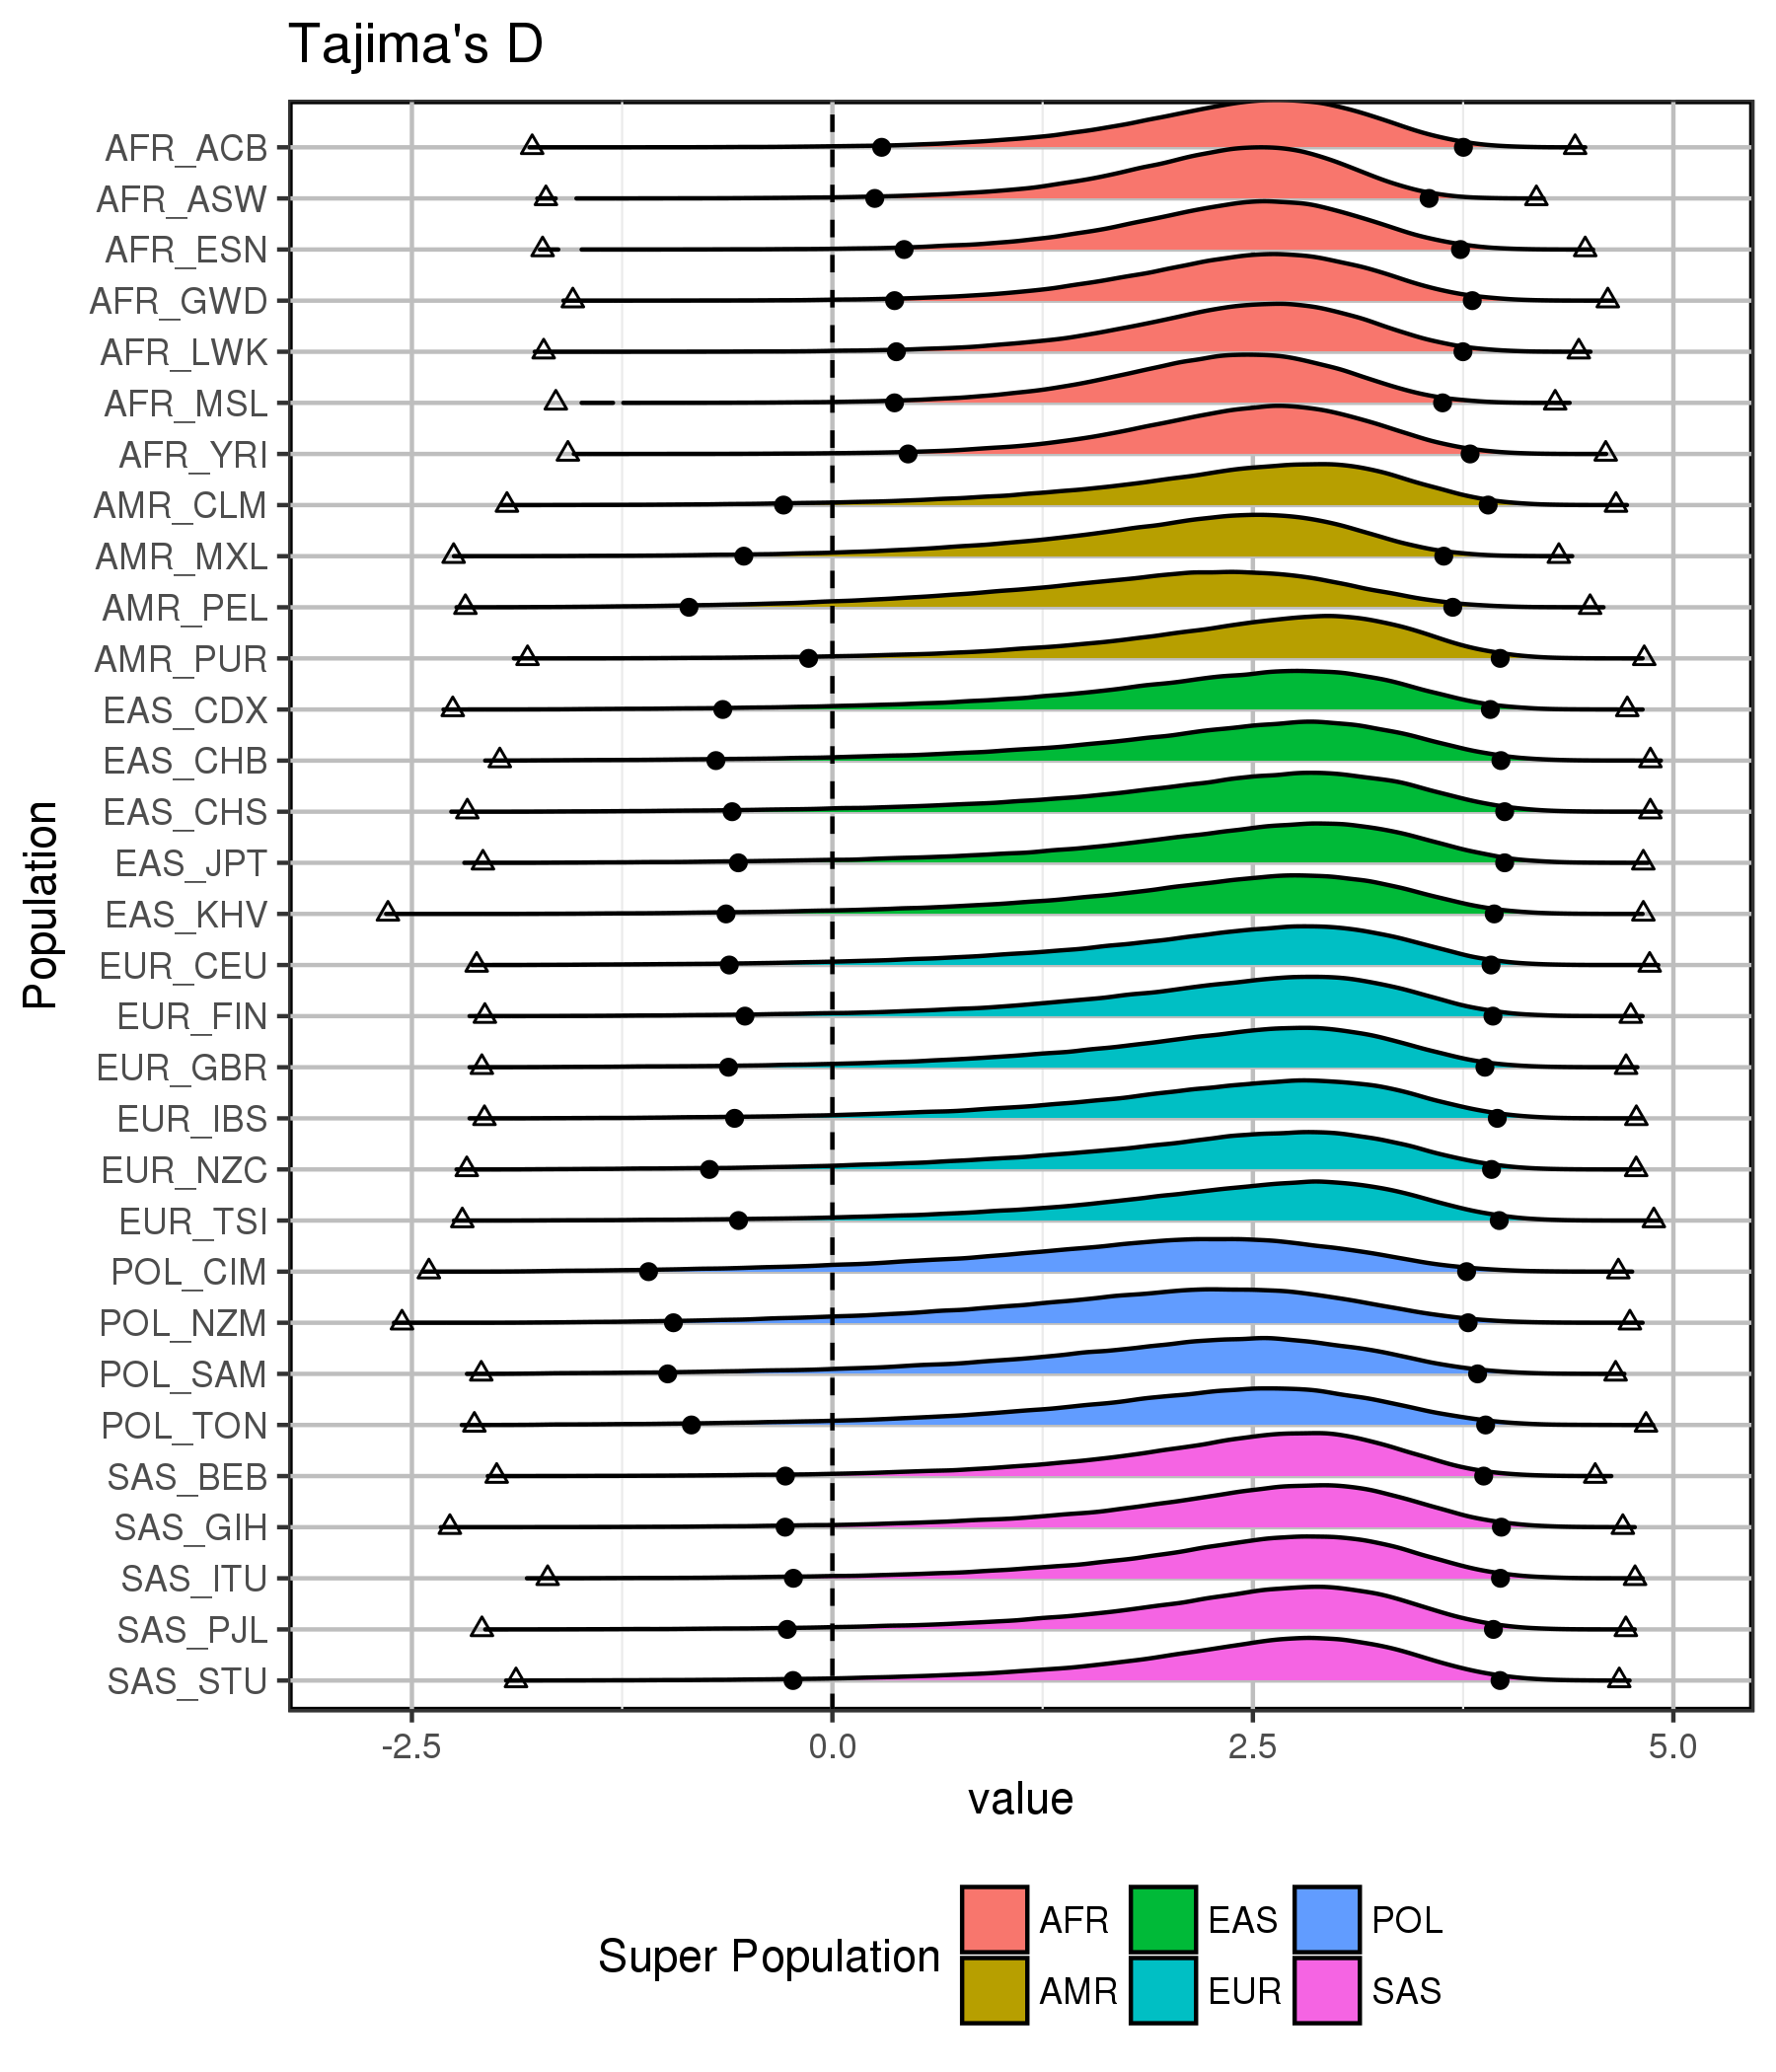
\includegraphics{_bookdown_files/images/04_clustering/td_densities} \caption[Plot of the distribution of \gls{td} by population]{Plot of the distribution of \gls{td} by population.
Triangles indicate the minimum and maximum values. Dots indicate the
1\textsuperscript{st} and 99\textsuperscript{th} percentiles for each
population.}\label{fig:tdDensity}
\end{figure}






\begin{figure}
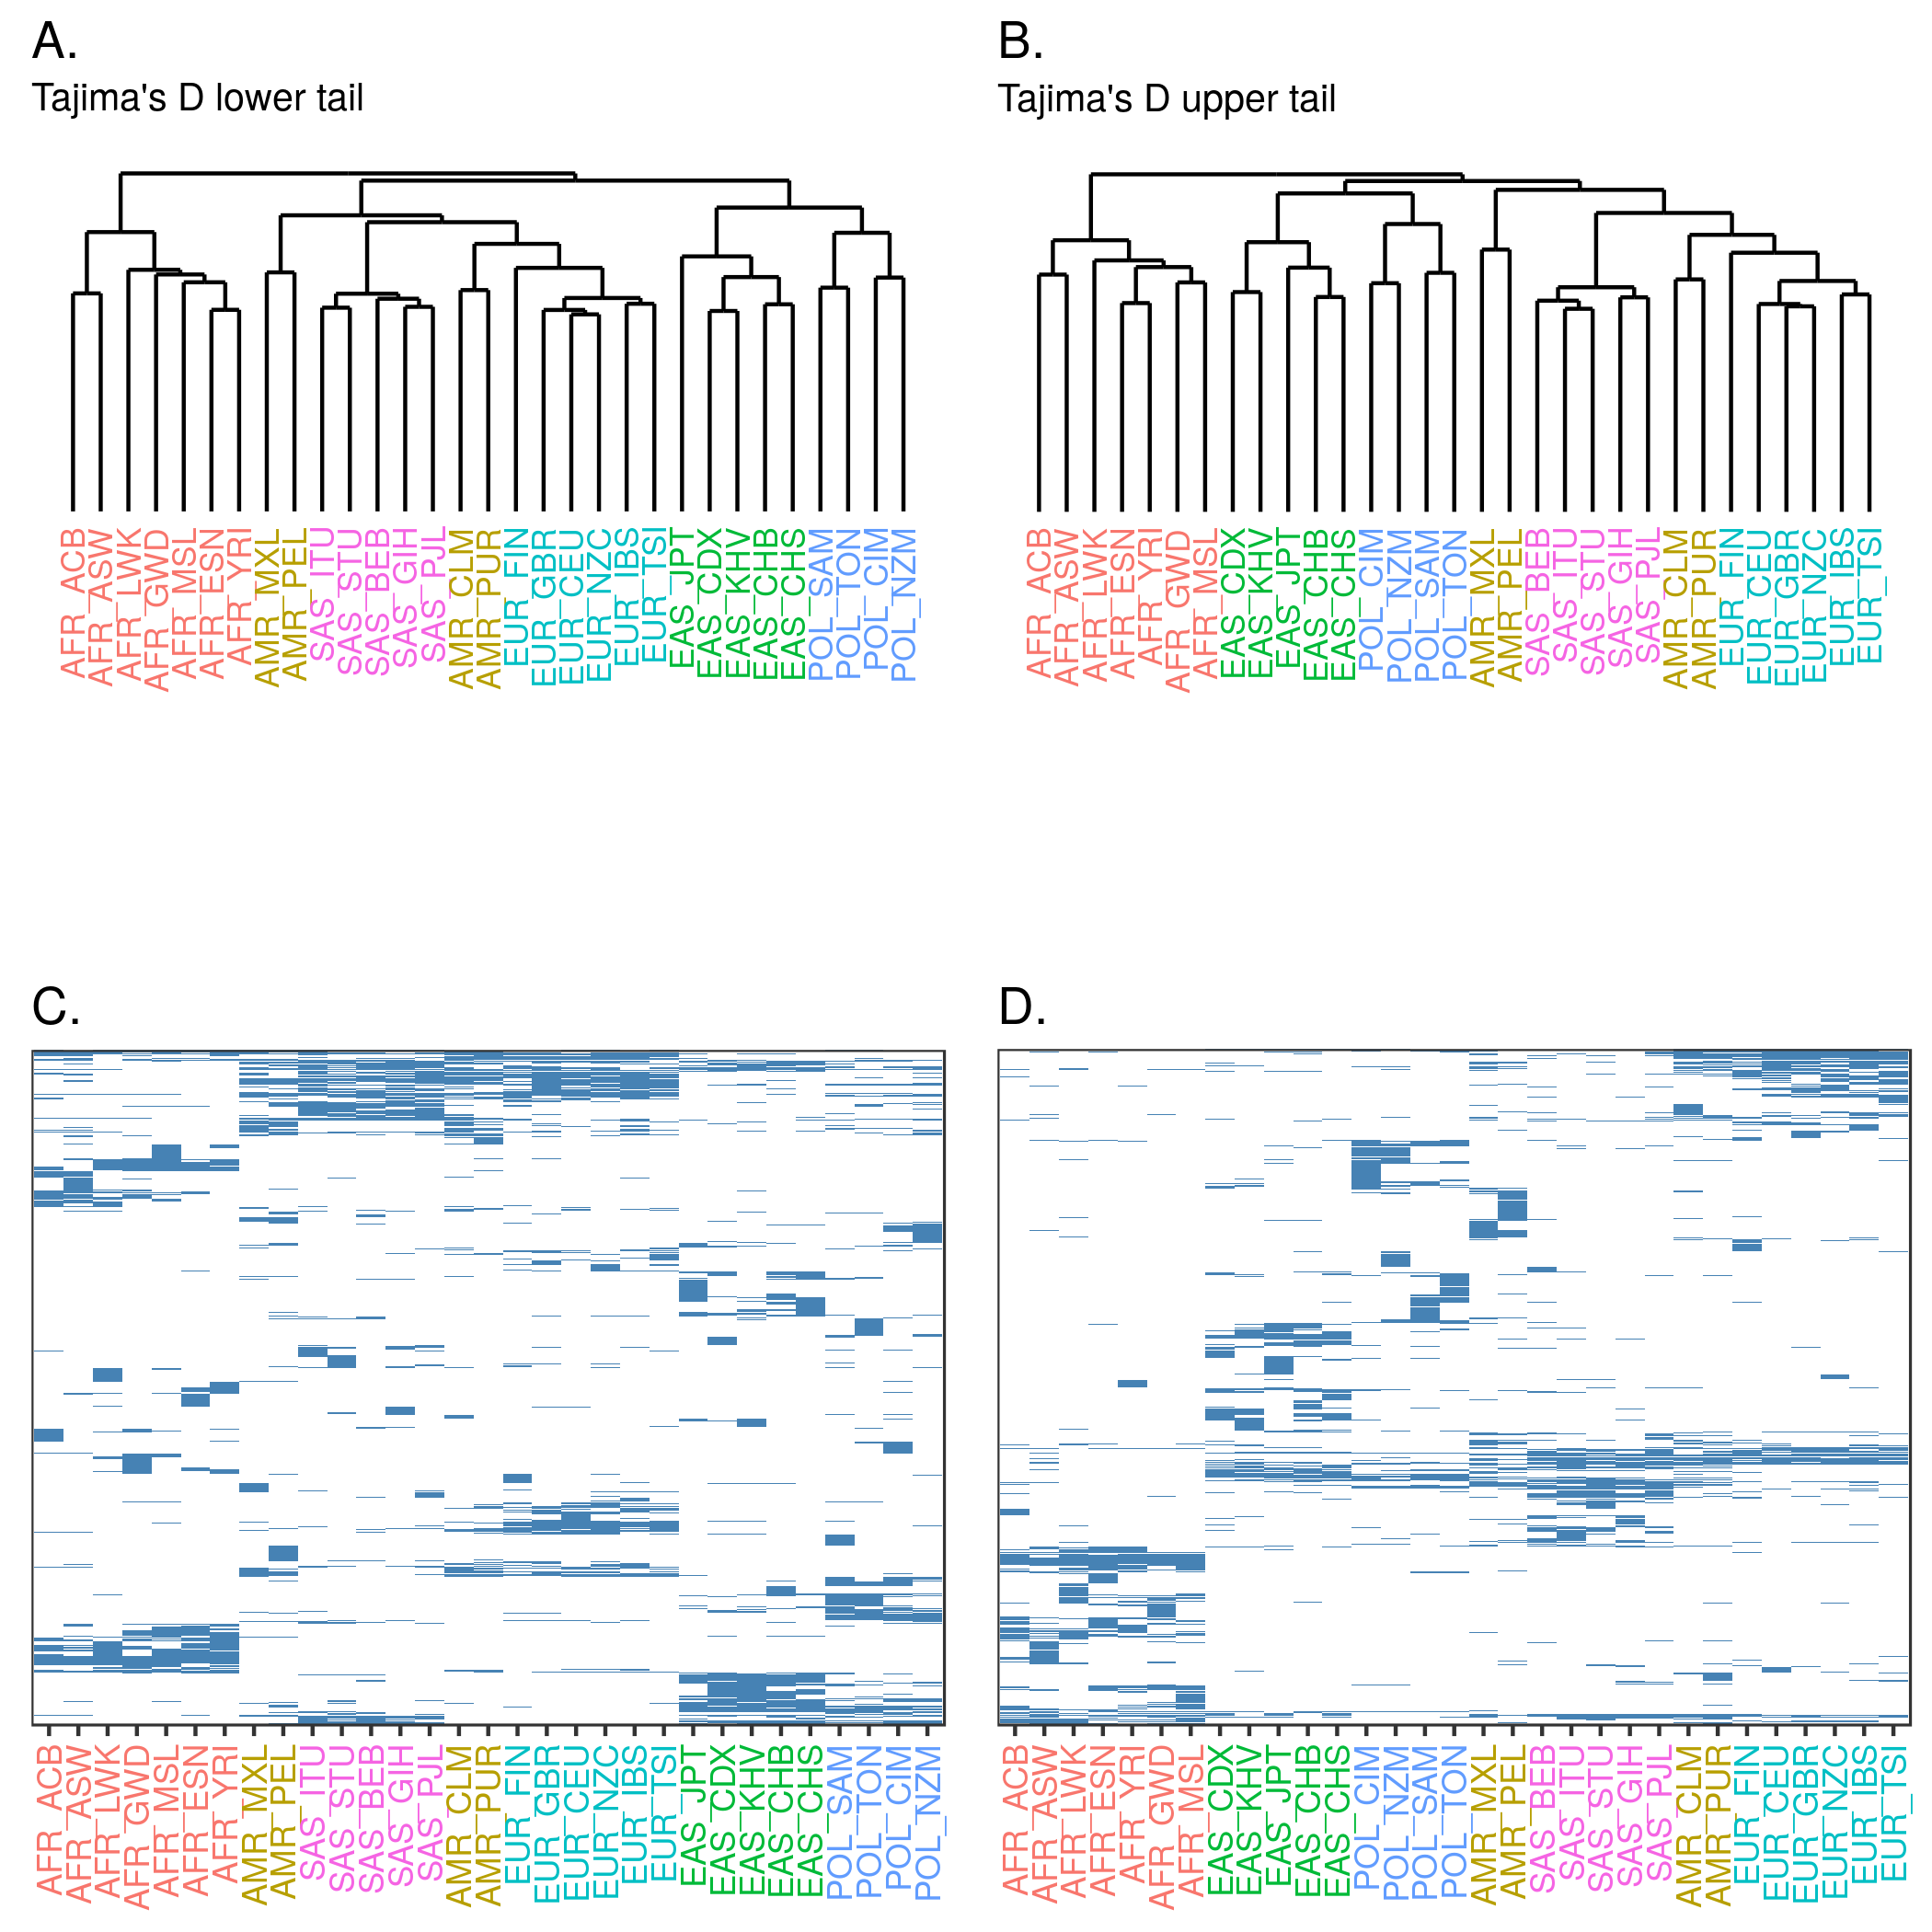
\includegraphics[width=6in]{images/04_clustering/tdTop1000} \caption[Hierarchical clustering of \gls{td} using the upper and lower 1\% of the distribution.]{Hierarchical clustering of \gls{td} using the upper and
lower 1\% of the distribution. \textbf{A} and \textbf{B} Dendrograms
representing the clusters of \gls{td} lower and upper tails
respectively, using hierarchical clustering with Euclidean distance and
complete linkage, and coloured by super population. \textbf{C} and
\textbf{D} Plots representing the windows present in each population
from the lower and upper tails respectively. A blue line represents
presence of a window, white represents the absence of a window in the
1\% of the distribution for a population.}\label{fig:tdTop1000}
\end{figure}











The clustering of the individual populations for the 1\% most extreme
values from each of the lower and upper tails of the \gls{td}
distribution both showed the East/West split in the Polynesians (Figure
\ref{fig:tdTop1000}). But the clustering also showed that the Polynesian
populations were most similar to each other. Both tails placed the
Polynesian cluster closest to the \gls{eas} cluster, consistent with the
migration history. The main groupings are of the populations that were
designated as the same super population, although the \gls{amr} super
population in both tails has been split into two. The mean number of
unique windows per population was 274.5 (SD 153.1) in the upper tail,
compared with 202.4 (SD 101.2) in the lower tail, indicating a higher
degree of window sharing in the 1\textsuperscript{st} percentiles of
populations. The groupings for both the upper and lower tails
exclusively grouped each of the \gls{afr}, \gls{sas} and \gls{pol} super
populations. The \gls{amr} super population was split into an exclusive
group of \gls{mxl} and \gls{pel}, and a group of \gls{clm} and \gls{pur}
which was shared with the \gls{eur} super population. All clusters,
except the \gls{amr} - \gls{eur} cluster, were each exclusive to a
single super population.

\paragraph{\texorpdfstring{Clustering Tajima's \emph{D}
1\textsuperscript{st}
percentile}{Clustering Tajima's D 1st percentile}}\label{clustering-tajimas-d-1st-percentile}

In the lower tail, the number of windows that were unique to the
Polynesian super population was 2188, representing 11.1\% of all windows
in the lower tail that were used. This compared to super population
unique window numbers of 4825, 1085, 2114, 1250, 1119 for the \gls{afr},
\gls{amr}, \gls{eas}, \gls{eur}, and \gls{sas} super populations
respectively. Of the unique windows for Polynesian populations, 267 were
specific to \gls{cim}, 266 were specific to \gls{nzm}, 300 were specific
to \gls{sam}, and 404 were specific to \gls{ton}. The Eastern
Polynesians had 699 unique windows with 166 of those shared between
\gls{cim} and \gls{nzm}, whereas the Western Polynesians had 950
windows, with 246 shared between \gls{sam} and \gls{ton}. There were 314
windows where all the Polynesian populations shared a window with a
non-Polynesian population. And 3130 windows, intersecting 1268 genes,
where at least one Polynesian population shared a window with a
non-Polynesian population (Table \ref{tab:polTdNegGenes}). There were 32
genes that had windows that were in the 1\textsuperscript{st} percentile
for all four Polynesian populations. Cell signalling as an immune
response, such as the Toll-like receptor cascades, were the main
pathways this list of genes covered, although this was largely due to
\emph{PPP2CB} and \emph{NOD1}. Two other genes in the list were
\emph{CCR3} and \emph{ARL15}, both of which are associated with obesity
related traits \citep{comuzzie2012novel, shungin2015genetic}, and the
latter also associated with \gls{t2d} \citep{mahajan2014genome}.

\paragraph{\texorpdfstring{Clustering Tajima's \emph{D}
99\textsuperscript{th}
percentile}{Clustering Tajima's D 99th percentile}}\label{clustering-tajimas-d-99th-percentile}

The upper tail had a total of 3036 windows, or 13.5\% that were unique
to the Polynesian populations. This compares to super population unique
window numbers of 4626 (\gls{afr}), 1774 (\gls{amr}), 2476 (\gls{eas}),
1952 (\gls{eur}), 1274 (\gls{sas}). Eastern Polynesians contributed 985
unique windows, with \gls{cim} having 491 unique windows and \gls{nzm}
having 494 windows. The Western Polynesians had 1279 unique windows. 497
were from only \gls{sam} and 533 from only \gls{ton}. There were 291
windows where all the Polynesian populations shared a window with a
non-Polynesian population. And 2807 windows, intersecting 1098 genes,
where at least one Polynesian population shared a window with a
non-Polynesian population (Table \ref{tab:polTdPosGenes}).

In both tails the clustering was being driven by a small subset of the
regions; this can be seen in Figures \ref{fig:tdTop1000} C and D, where
most of the regions that the Polynesian populations have are not shared
with the other populations. It can also be seen that the regions that
the Polynesian populations do have in common are also shared with the
\gls{eas} populations. This is reflected in the dendrograms in Figures
\ref{fig:tdTop1000} A and B.

\paragraph{\texorpdfstring{Metabolic disease-associated genes in the
extremes of Tajima's
\emph{D}}{Metabolic disease-associated genes in the extremes of Tajima's D}}\label{metabolic-disease-associated-genes-in-the-extremes-of-tajimas-d}

Specifically focusing on the 465 genes that were associated with urate,
gout, obesity, \gls{t2d}, kidney disease, and metabolic syndrome from
the \gls{gwas} catalog (Tables \ref{tab:gwascatref} and
\ref{tab:gwasgenes}), from the clustering of the extremes, there were a
total of 32 genes that had at least one of the Polynesian populations
having at least one window in the 1\textsuperscript{st} percentile. This
dropped to 6 genes that had windows in the 1\textsuperscript{st}
percentile for at least one Polynesian population, and also in the
1\textsuperscript{st} percentile of other populations. Some examples of
this were \emph{CCR3}, which had windows in the 1\textsuperscript{st}
percentile for all four Polynesian populations, and the same windows
were also in the 1\textsuperscript{st} percentile as the \gls{eas}
populations of \gls{cdx} and \gls{khv}. \emph{ARL15} had windows that
were only from the four Polynesian populations. And \emph{DNAH10} had
windows that were in the 1\textsuperscript{st} percentile of the
\gls{eas} populations except \gls{cdx}, as well as the Eastern
Polynesian populations, \gls{cim} and \gls{nzm}. In the
99\textsuperscript{th} percentile there were 39 genes associated with
the metabolic diseases that had windows in the Polynesian populations,
of those, 9 genes had windows in the 99th percentile for Polynesians and
the 99\textsuperscript{th} percentile of other populations. Some
examples include \emph{ADCY3} which had multiple windows with \gls{pol},
\gls{eur}, \gls{eas}, and \gls{sas}. And \emph{NEGR1} which had windows
from both the \gls{eas} and \gls{pol} populations.

\subsubsection{\texorpdfstring{Fay and Wu's
\emph{H}}{Fay and Wu's H}}\label{fay-and-wus-h-1}

\paragraph{\texorpdfstring{Fay and Wu's \emph{H}
distributions}{Fay and Wu's H distributions}}\label{fwhDist}

Comparing genome-wide \gls{fwh} revealed that the \gls{pol} super
population had the lowest mean (-1.283), 1\textsuperscript{st}
percentile (-6.395), median (-0.982), 99\textsuperscript{th} percentile
(1.162), and maximum values (1.732) (Figure \ref{fig:fwhDensity} and
Table \ref{tab:superGlobalSummaryFWH}). Within the \gls{pol} group, the
minimum \gls{fwh} value for a Polynesian population was from NZM,
whereas the maximum value was from SAM. \gls{eas} was the second lowest
for mean (-1.040), 1\textsuperscript{st} percentile (-5.977), median
(-0.743), and 99\textsuperscript{th} percentile (1.232), but had the
largest maximum (1.860). The \gls{eur} super population had both the
smallest minimum and largest range (14.850). The \gls{afr} super
population were the only group to have a positive mean (0.028), they
also had the smallest range and variation (SD 0.913). This indicates
that the \gls{afr} populations have a deficit of moderate-to-high
frequency derived alleles, whereas the \gls{pol} and \gls{eas}
populations have the most windows with the highest excess of
moderate-to-high frequency derived alleles.

\begin{figure}
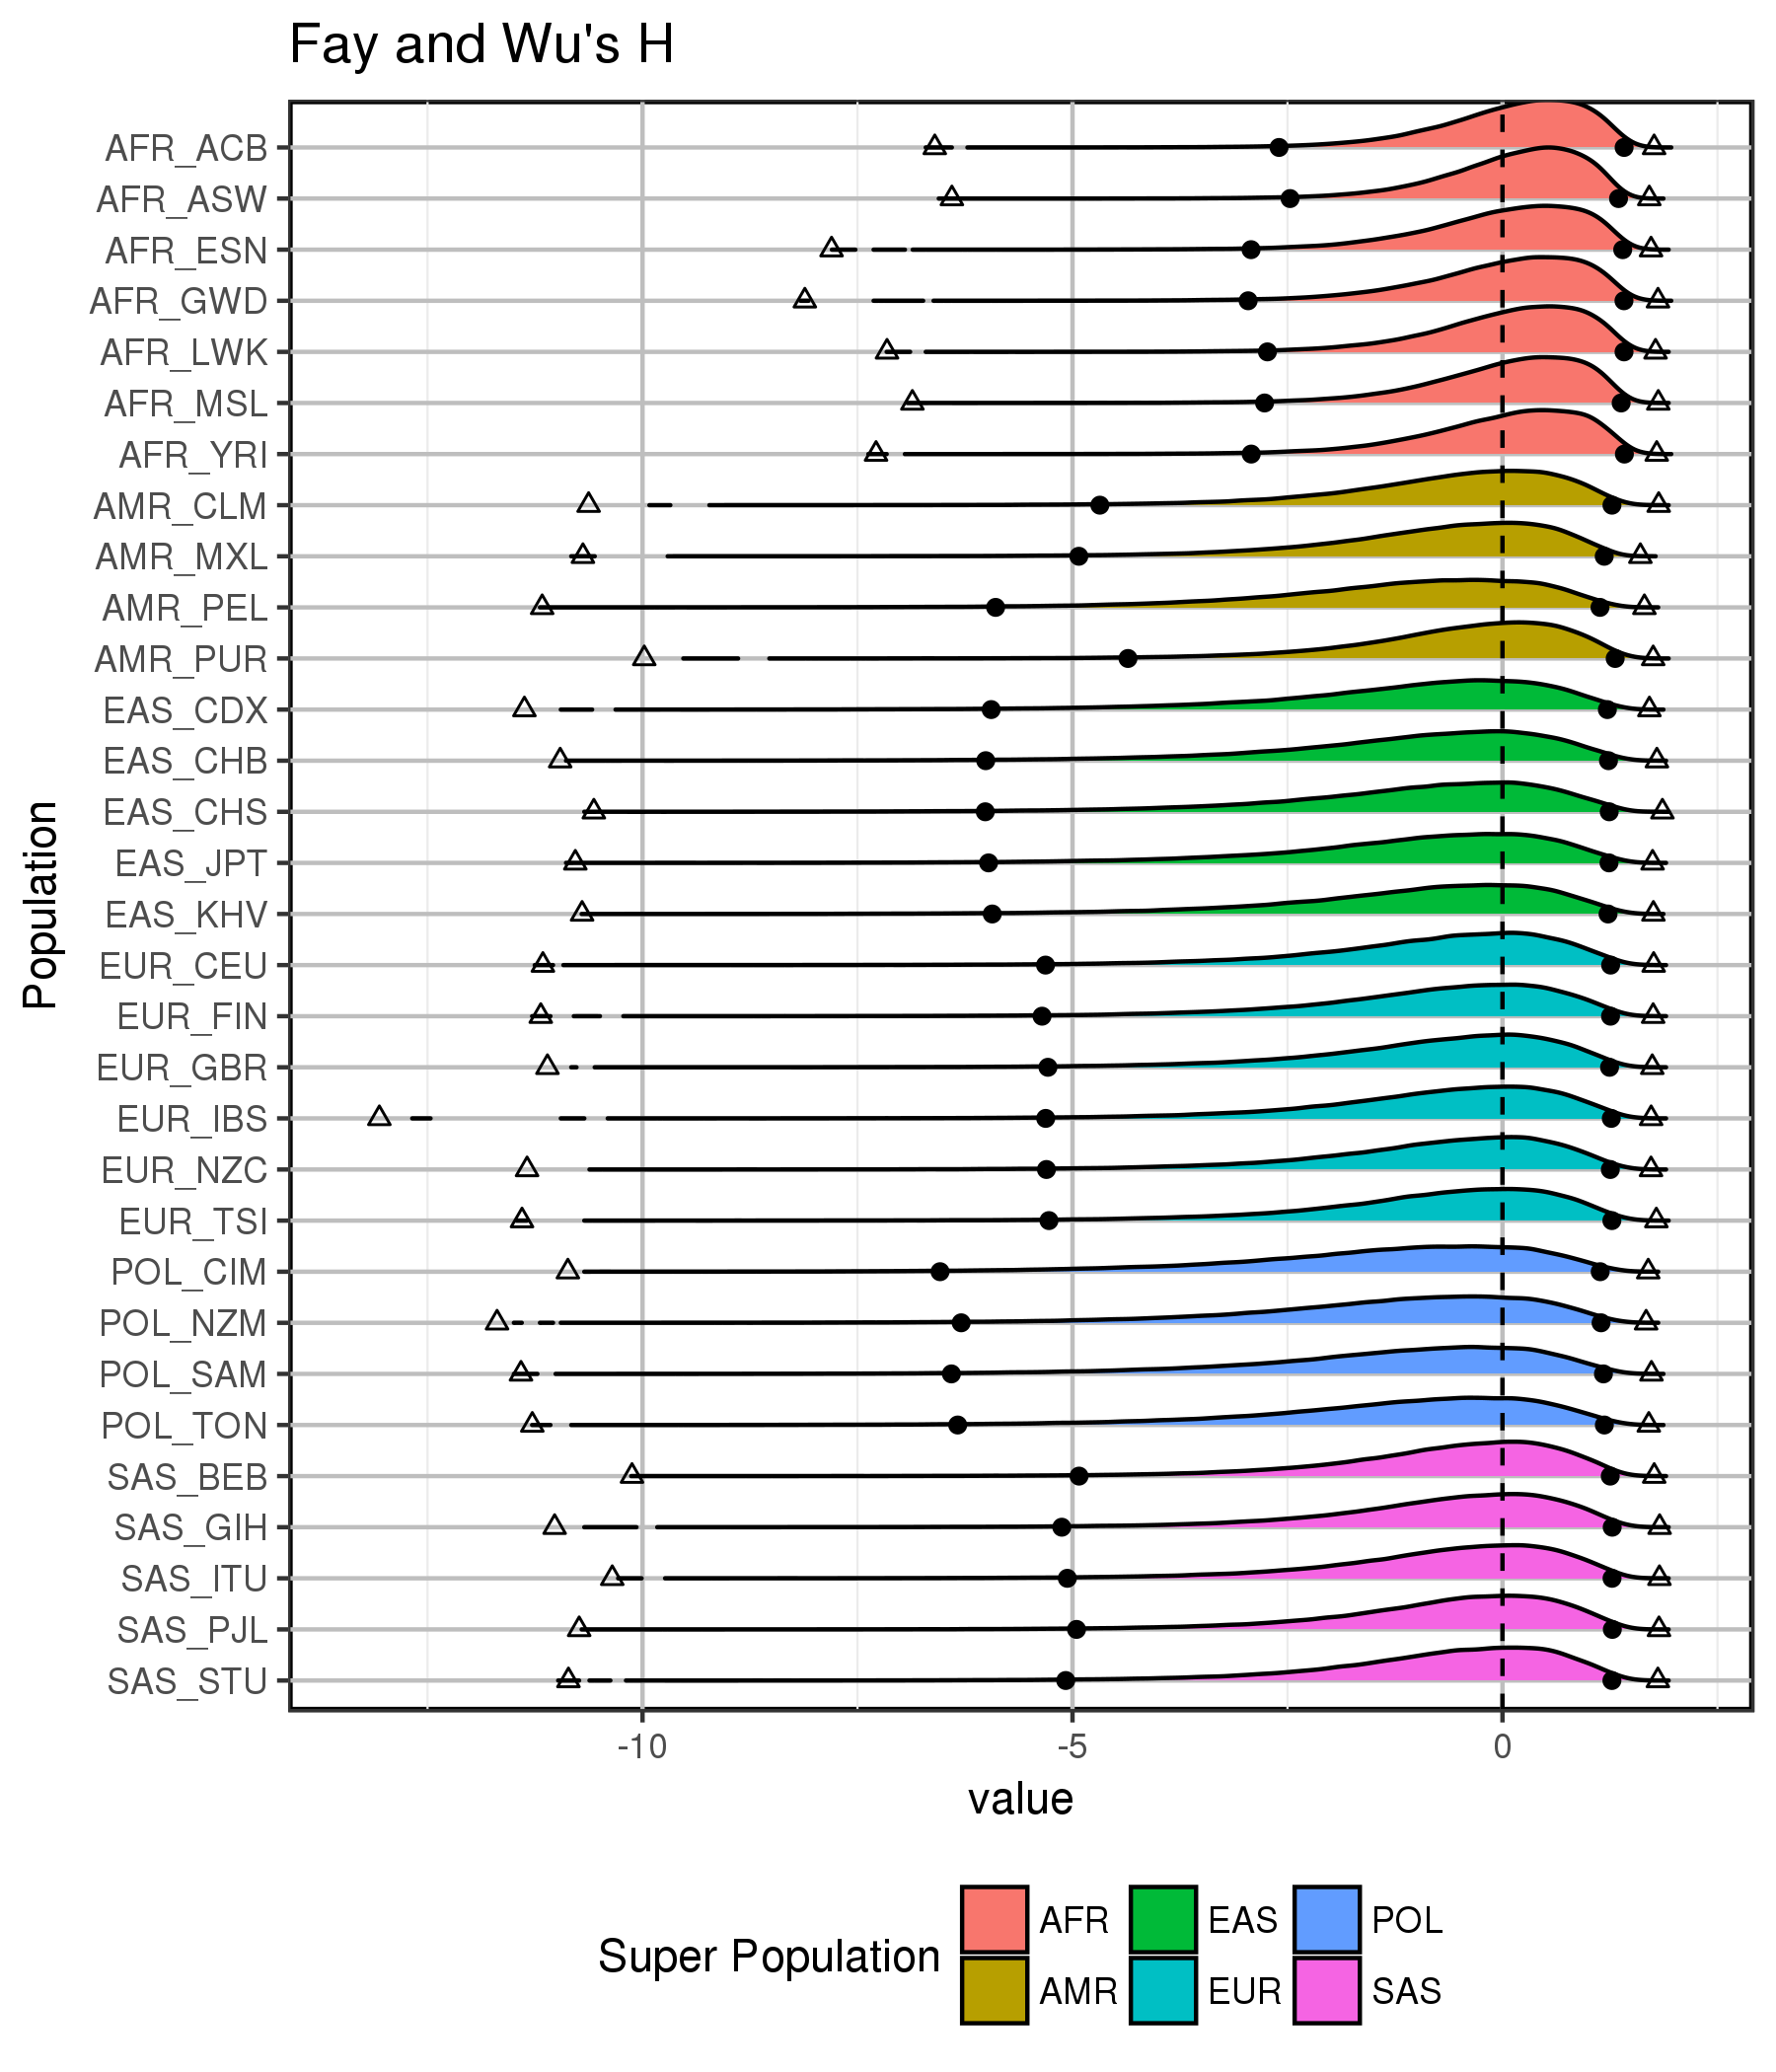
\includegraphics{_bookdown_files/images/04_clustering/fwh_densities} \caption[Plot of the distribution of \gls{fwh} by population.]{Plot of the distribution of \gls{fwh} by population.
Triangles indicate the minimum and maximum values. Dots indicate the
1\textsuperscript{st} and 99\textsuperscript{th} percentiles for each
population.}\label{fig:fwhDensity}
\end{figure}






\begin{table}

\caption{\label{tab:unnamed-chunk-16}\label{tab:superGlobalSummaryFWH} Summary statistics for \gls{fwh} by super population.}
\centering
\resizebox{\linewidth}{!}{
\begin{tabular}[t]{lrrrrrrr}
\toprule
Super Population & Mean & SD & Min & 1st Percentile & Median & 99th Percentile & Max\\
\midrule
AFR & 0.028 & 0.913 & -8.113 & -2.782 & 0.183 & 1.400 & 1.812\\
AMR & -0.761 & 1.366 & -11.167 & -5.098 & -0.507 & 1.240 & 1.817\\
EAS & -1.040 & 1.551 & -11.374 & -5.977 & -0.743 & 1.232 & 1.860\\
EUR & -0.812 & 1.415 & -13.060 & -5.306 & -0.546 & 1.259 & 1.789\\
POL & -1.283 & 1.648 & -11.692 & -6.395 & -0.982 & 1.162 & 1.732\\
SAS & -0.704 & 1.348 & -11.022 & -5.031 & -0.453 & 1.271 & 1.827\\
\bottomrule
\end{tabular}}
\end{table}











\begin{figure}
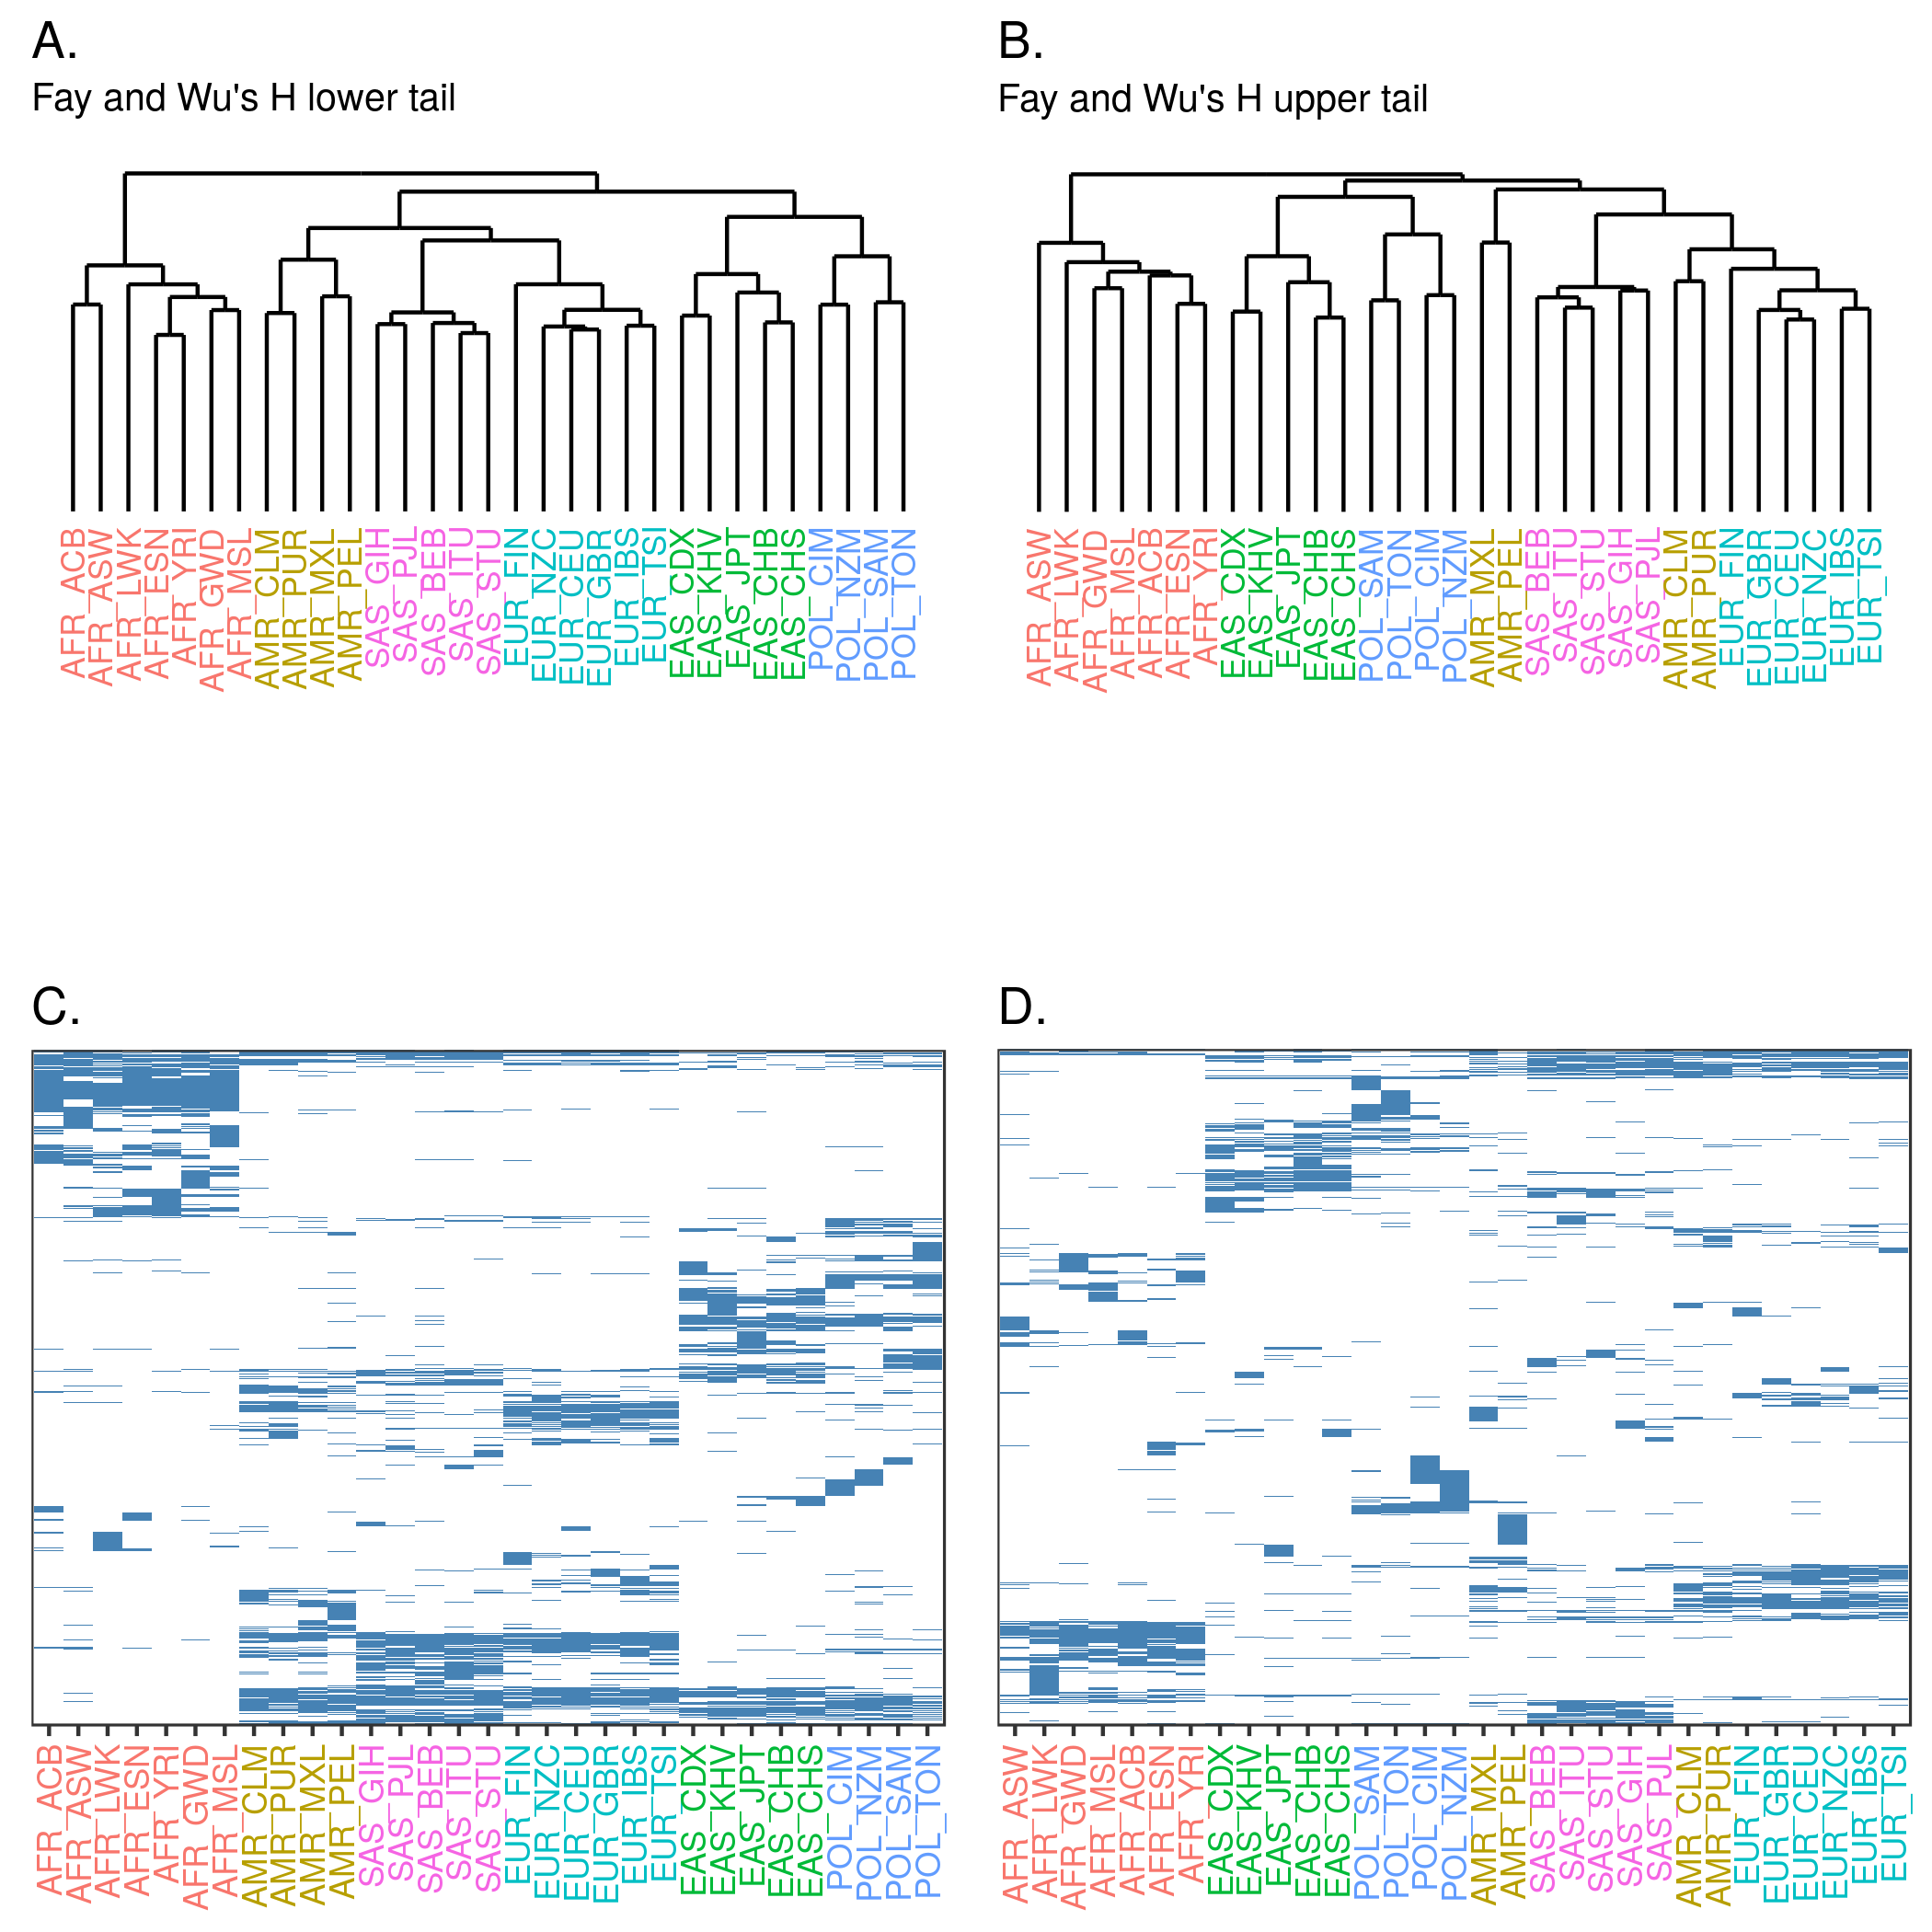
\includegraphics[width=6in]{images/04_clustering/fwhTop1000} \caption[Hierarchical clustering of \gls{fwh} using the upper and lower 1\% of the distribution.]{Hierarchical clustering of \gls{fwh} using the upper
and lower 1\% of the distribution. \textbf{A} and \textbf{B} Dendrograms
representing the clusters of \gls{fwh} lower and upper tails
respectively, using hierarchical clustering with Euclidean distance and
complete linkage, and coloured by super population. \textbf{C} and
\textbf{D} Plots representing the windows present in each population
from the lower and upper tails respectively. A blue line represents
presence of a window, white represents the absence of a window in the
1\% of the distribution for a population.}\label{fig:fwhTop1000}
\end{figure}

The clustering of \gls{fwh} (Figure \ref{fig:fwhTop1000}) had the main
groupings the same as the defined super population groups, with the
exception of the upper tail where the \gls{amr} super population was
split in half. The Polynesian populations were clustered together in
both the lower and upper tails for \gls{fwh}. In both tails the
Polynesian cluster also had the East/West split within the group. The
Polynesian population group was closest to the \gls{eas} populations
with 1631 windows from the upper tail and 2212 windows from the lower
tail in common between at least one Polynesian population and one
\gls{eas} population.

\paragraph{\texorpdfstring{Clustering Fay and Wu's \emph{H}
1\textsuperscript{st}
percentile}{Clustering Fay and Wu's H 1st percentile}}\label{clustering-fay-and-wus-h-1st-percentile}

The clustering of the lower tail assigned all the individuals into their
super populations and each of the groups were exclusive to their super
population. There were a total of 15,628 windows in the lower tail, with
1546 windows specific to Polynesian populations. This compared to 3767
windows for \gls{afr}, 679 windows for \gls{amr}, 1081 windows for
\gls{eur}, and 1375 windows for \gls{eas}. The Eastern Polynesian
populations had 561 windows, of those, 230 were specific to \gls{cim}
and 189 were specific to \gls{nzm}. The Western Polynesian populations
had 593 windows, with 156 specific to \gls{sam} and 283 specific to
\gls{ton}. The mean number of windows specific to an individual
population was 135.6 (SD 72.8) in the lower tail. There were 595 windows
with all Polynesians that also shared with a non-Polynesian population.
And 3208 windows, intersecting 885 genes with at least one Polynesian
population that also shared with a non-Polynesian population (Table
\ref{tab:polFwhNegGenes}). There were 38 genes that had windows that
were only in the four Polynesian populations and no others.

\paragraph{\texorpdfstring{Clustering Fay and Wu's \emph{H}
99\textsuperscript{th}
percentile}{Clustering Fay and Wu's H 99th percentile}}\label{clustering-fay-and-wus-h-99th-percentile}

In the upper tail of the \gls{fwh} distribution, the clustering assigned
all of the individual populations into their super populations with only
\gls{amr} being split. The \gls{clm} and \gls{pur} populations were
clustered as part of the \gls{eur} group. Exclusivity was also high with
all clusters except the \gls{eur} - \gls{amr} being exclusive to a
single super population. Of the 20,659 windows, 2545 windows were from
Polynesian populations only. The Eastern Polynesian populations had 1119
specific windows, of those, 404 were unique to \gls{cim} and 371 were
unique to \gls{nzm}. The Western Polynesian populations had 925 unique
windows, of these, 305 were specific to \gls{sam} and 332 specific to
\gls{ton}. The mean number of unique windows for all populations was
226.4 (SD 144.1). There were 344 windows with all Polynesians that also
shared with a non-Polynesian population. And 2731 windows, intersecting
1176 genes, with at least one Polynesian population that also shared
with a non-Polynesian population (Table \ref{tab:polFwhPosGenes}).

The 1\textsuperscript{st} percentile has many of the regions in the
Polynesian populations in common with the \gls{eas} populations (Figure
\ref{fig:fwhTop1000}). Whereas, in the 99\textsuperscript{th} percentile
there were more regions that were only from the Polynesian populations
that were not in common with any other populations. This shows that the
regions with high frequency derived alleles are in common with the
\gls{eas} populations, indicating they possibly originated prior to the
Polynesian migration.

\paragraph{\texorpdfstring{Metabolic disease-associated genes in the
extremes of Fay and Wu's
\emph{H}}{Metabolic disease-associated genes in the extremes of Fay and Wu's H}}\label{metabolic-disease-associated-genes-in-the-extremes-of-fay-and-wus-h}

Of the genes that were in the windows of the 1\textsuperscript{st}
percentile, there were 30 genes that were in the list of genes of
metabolic disease associated genes and also had windows that intersected
them from the Polynesian populations. Thirteen of those genes were for
windows from Polynesian populations, as well as others. Some examples of
these genes were \emph{RASA2} and \emph{ERBB4}, and both are associated
with obesity traits and involved in signalling pathways. \emph{RASA2}
had windows only from \gls{cim} and \gls{nzm}. \emph{ERBB4} had windows
from all four Polynesian populations, as well as the populations of
\gls{eas} - except \gls{jpt}.

There were 25 genes that were in the 99\textsuperscript{th} percentile
that were also in the list of genes of metabolic disease associated
genes. Some examples of genes that had windows in both Polynesian and
other populations in the 99\textsuperscript{th} percentile include
\emph{SHROOM3}, \emph{RBMS1}, and \emph{UBE2E2}. \emph{SHROOM3} was an
example of a gene that had windows in common from all the other super
populations, except \gls{eas}. \emph{RBMS1} had multiple windows for
across all Polynesian populations, but not other super populations. And
\emph{UBE2E2} had multiple windows across the Polynesian populations, as
well as the populations of \gls{eas} and \gls{sas}. \emph{SHROOM3} was
an example of a gene associated with kidney disease, with its role being
in the development of the kidney \citep{Khalili2016}.

\subsubsection{\texorpdfstring{Fu and Li's
\emph{F}}{Fu and Li's F}}\label{fu-and-lis-f-1}

\paragraph{Fu and Li's distributions}\label{flfDist}

The distributions of \gls{flf} were all centred above zero, with the
lowest mean being that of \gls{pol} at 1.719 (Figure
\ref{fig:flfDensity} and Table \ref{tab:superGlobalSummaryFLF}). The
\gls{pol} populations also had the lowest 1\textsuperscript{st}
percentile (-0.685), median (1.844), and 99\textsuperscript{th}
percentile (2.970). Conversely, the \gls{sas} populations had the
highest mean (2.012), median (2.104), and were equal with the \gls{afr}
populations with the highest minimum (-4.068). The \gls{afr} populations
were the only group to have a positive 1\textsuperscript{st} percentile
(0.243). The \gls{eas} populations had the lowest minimum (-5.262), but
the highest 99\textsuperscript{th} percentile (3.110) and the largest
range (9.195). This pattern was similar to what was seen with \gls{td}.






\begin{figure}
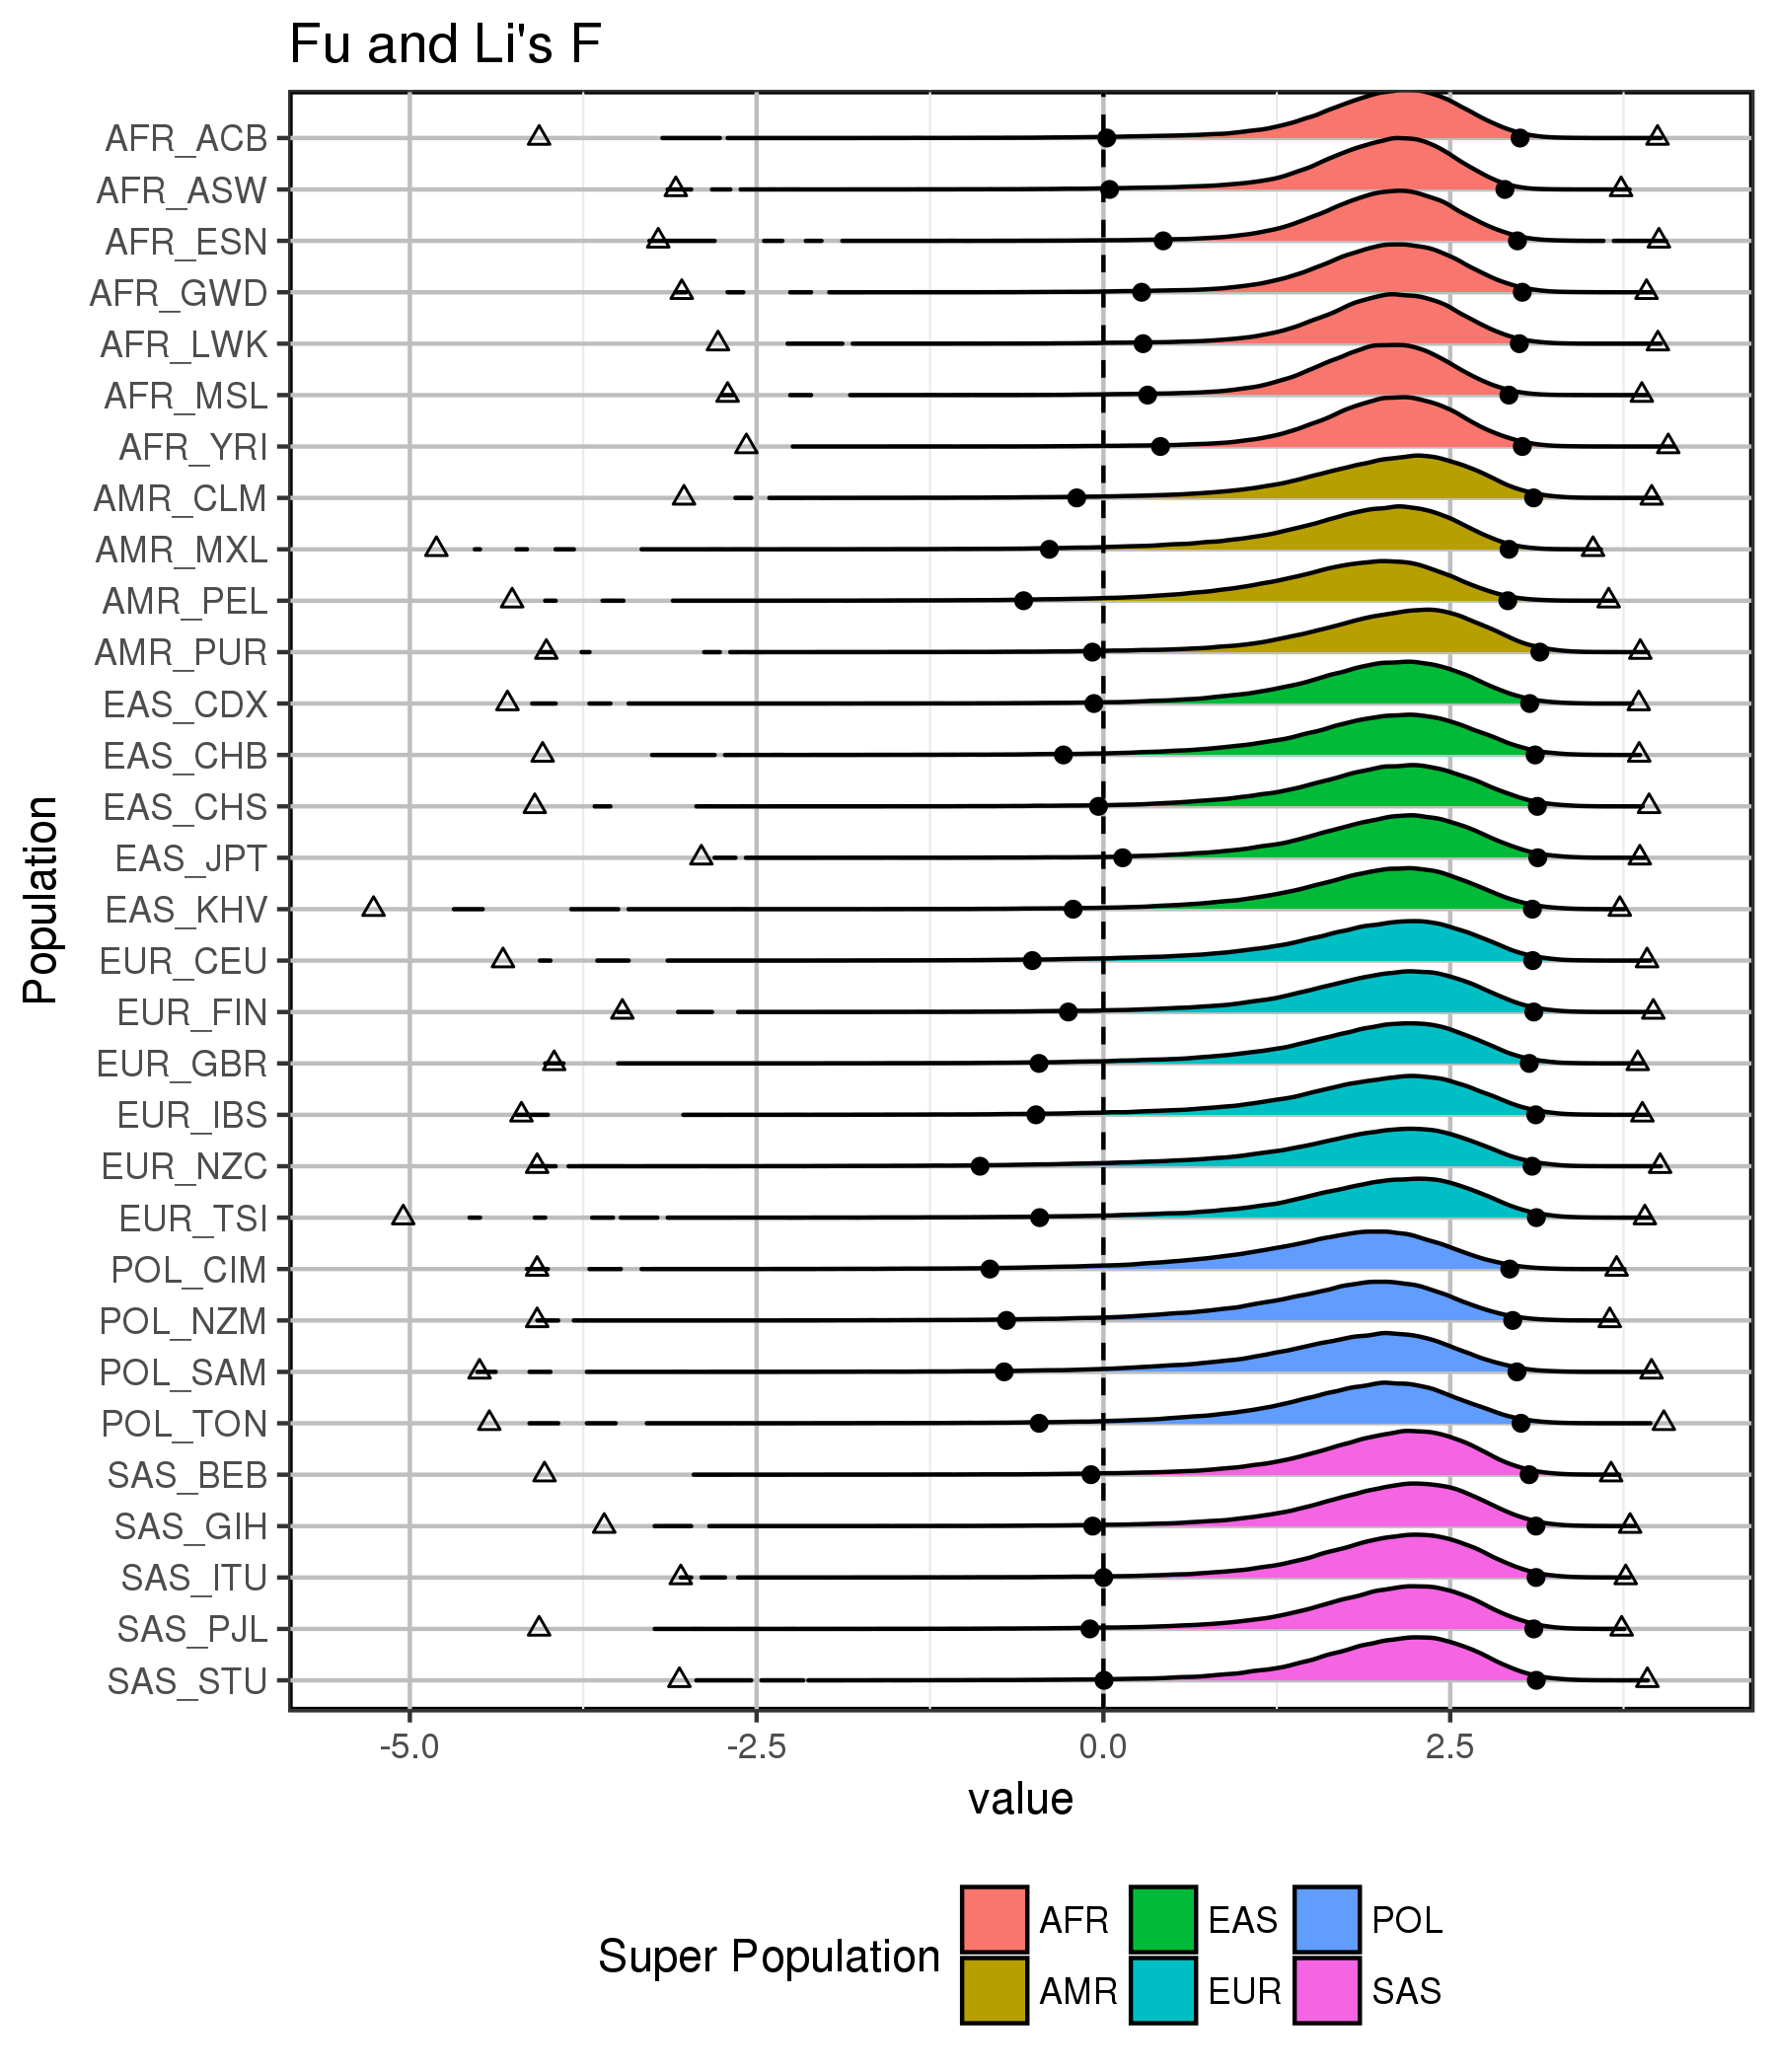
\includegraphics{_bookdown_files/images/04_clustering/flf_densities} \caption[Plot of the distribution of \gls{flf} by population.]{Plot of the distribution of \gls{flf} by population.
Triangles indicate the minimum and maximum values. Dots indicate the
1\textsuperscript{st} and 99\textsuperscript{th} percentiles for each
population.}\label{fig:flfDensity}
\end{figure}

\begin{table}

\caption{\label{tab:unnamed-chunk-21}\label{tab:superGlobalSummaryFLF} Summary statistics for \gls{flf} by super population.}
\centering
\resizebox{\linewidth}{!}{
\begin{tabular}[t]{lrrrrrrr}
\toprule
Super Population & Mean & SD & Min & 1st Percentile & Median & 99th Percentile & Max\\
\midrule
AFR & 1.992 & 0.543 & -4.068 & 0.243 & 2.050 & 2.982 & 4.072\\
AMR & 1.891 & 0.694 & -4.809 & -0.342 & 1.998 & 3.055 & 3.953\\
EAS & 1.955 & 0.663 & -5.262 & -0.108 & 2.044 & 3.110 & 3.934\\
EUR & 1.899 & 0.744 & -5.048 & -0.528 & 2.025 & 3.100 & 4.013\\
POL & 1.719 & 0.754 & -4.498 & -0.685 & 1.844 & 2.970 & 4.040\\
SAS & 2.012 & 0.643 & -4.068 & -0.055 & 2.104 & 3.107 & 3.921\\
\bottomrule
\end{tabular}}
\end{table}











\begin{figure}
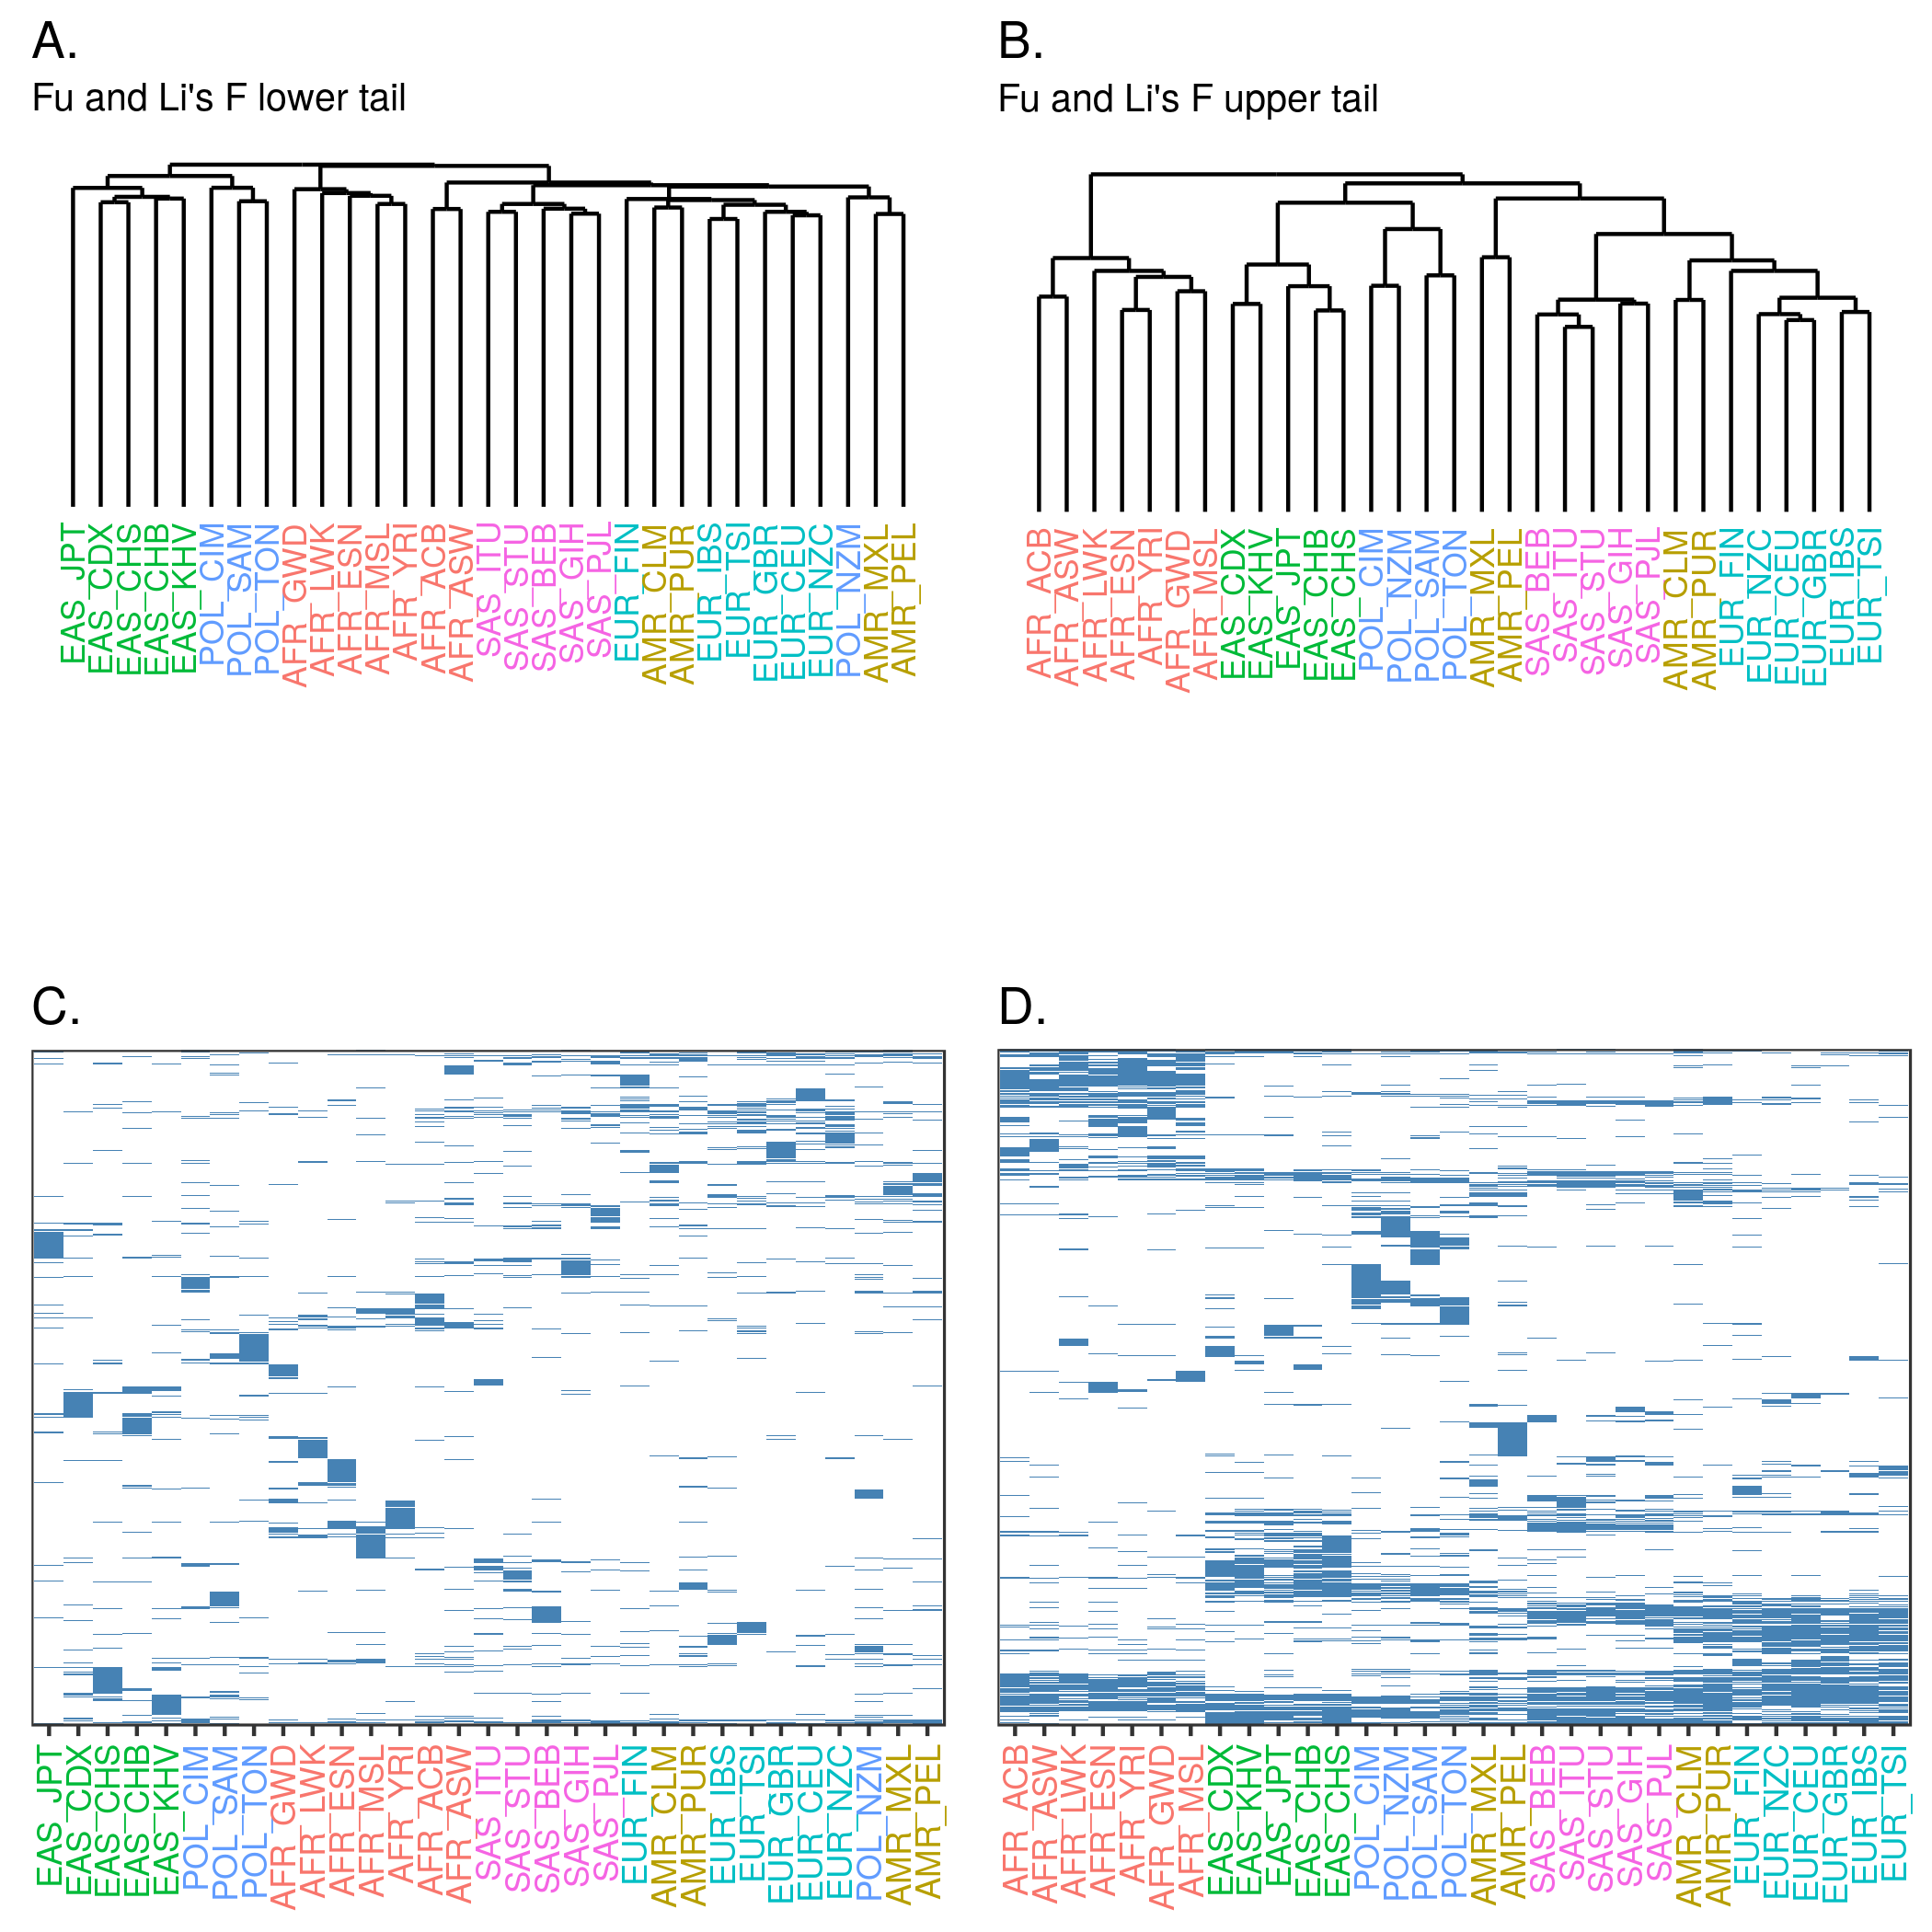
\includegraphics[width=6in]{images/04_clustering/flfTop1000} \caption[Hierarchical clustering of \gls{flf} using the upper and lower 1\% of the distribution.]{Hierarchical clustering of \gls{flf} using the upper
and lower 1\% of the distribution. \textbf{A} and \textbf{B} Dendrograms
representing the clusters of \gls{flf} lower and upper tails
respectively, using hierarchical clustering with Euclidean distance and
complete linkage, and coloured by super population. \textbf{C} and
\textbf{D} Plots representing the windows present in each population
from the lower and upper tails respectively. A blue line represents
presence of a window, white represents the absence of a window in the
1\% of the distribution for a population.}\label{fig:flfTop1000}
\end{figure}

Clustering on the 1\% \gls{flf} from each tail of the distribution
(Figure \ref{fig:flfTop1000}) had 13851 windows in the upper tail
(Figure \ref{fig:flfTop1000} B and D) and 30798 windows in the lower
tail (Figure \ref{fig:flfTop1000} A and C). The mean number of unique
windows per population was 120.6 (SD 102.8) in the upper tail, compared
with 467.2 (SD 202.1) in the lower tail. Both tails clustered the
\gls{eas} populations into their own exclusive cluster.

\paragraph{\texorpdfstring{Clustering Fu and Li's \emph{F}
1\textsuperscript{st}
percentile}{Clustering Fu and Li's F 1st percentile}}\label{clustering-fu-and-lis-f-1st-percentile}

Clustering on the lower tail windows grouped the majority of the
individual populations together into their super populations. The
Polynesian populations were grouped together as a West Polynesian group
and the \gls{cim} population. The \gls{nzm} population was grouped with
the \gls{mxl} and \gls{pel} as part of a larger group with the \gls{eur}
super population. Exclusivity of clusters was reasonable with four of
six being exclusive. There were a total of 30,798 windows with 2722
windows specific to Polynesian populations. This compared to 6337
windows for \gls{afr}, 1322 windows for \gls{amr}, 2635 windows for
\gls{eur}, and 4168 windows for \gls{eas}. The Eastern Polynesian
populations had a total of 926 unique windows, 483 were unique to
\gls{cim} and 407 were unique to \gls{nzm}. The Western Polynesian
populations had 1538 unique windows. Of these, 565 were unique to
\gls{sam} and 811 to \gls{ton}. There were 15 genes that overlapped
windows in the 1\textsuperscript{st} percentiles of all four Polynesian
populations (Table \ref{tab:polFlfNegGenes}). Of these genes, three
(\emph{OR4C11}, \emph{OR4C15}, and \emph{OR4C16}) were involved with the
significantly enriched ``Olfactory transduction\_Homo
sapiens\_hsa04740'' pathway (adjusted P = 0.044).

\paragraph{\texorpdfstring{Clustering Fu and Li's \emph{F}
99\textsuperscript{th}
percentile}{Clustering Fu and Li's F 99th percentile}}\label{clustering-fu-and-lis-f-99th-percentile}

Clustering on the windows from the upper tail put the super populations
into their own groups, but also split the \gls{amr} populations into two
separate groups. The Polynesian populations were also clustered into an
East/West split of 2 separate exclusive clusters. Exclusivity of
clusters was high with five of the six clusters being exclusive to a
single super population, however one cluster contained half of the
\gls{amr} populations (\gls{clm} and \gls{pur}) and all of the \gls{eur}
and \gls{sas} populations. There were a total of 13,851 windows with
1804 windows specific to Polynesian populations. This compared to 2020
windows for \gls{afr}, 896 windows for \gls{amr}, 777 windows for
\gls{eur}, and 953 windows for \gls{eas}. The Eastern Polynesian
populations had a total of 795 unique windows with 314 only from
\gls{cim} and 228 from \gls{nzm}. From the Western Polynesian
populations there were 687 specific windows. There were 267 specific to
\gls{sam} and 276 specific to \gls{ton}. There were 101 genes that
overlapped windows in the 99\textsuperscript{th} percentiles of all four
Polynesian populations (Table \ref{tab:polFlfPosGenes}).

\paragraph{\texorpdfstring{Metabolic disease associated genes in the
extremes of Fu and Li's
\emph{F}}{Metabolic disease associated genes in the extremes of Fu and Li's F}}\label{metabolic-disease-associated-genes-in-the-extremes-of-fu-and-lis-f}

There were 50 genes that were in the list of genes of metabolic disease
associated genes and also had windows in the 1\textsuperscript{st}
percentile, that intersected them from the Polynesian populations. Some
examples of these genes were \emph{MAFC1}, \emph{DNAH10} and
\emph{SLC2A9}. \emph{MAFC1} had six windows, some of which were in
common with the \gls{amr} and \gls{afr} populations. \emph{DNAH10} had
18 windows, with about half being in common with the populations of
\gls{eur}, \gls{eas}, \gls{sas}, and \gls{amr}. The urate transporter
\emph{SLC2A9} had multiple significant windows in \gls{ton}, \gls{jpt},
and \gls{chb}.

There were 41 of genes that were in the 99\textsuperscript{th}
percentile for Polynesians. Some examples were \emph{HLA-B},
\emph{PTPRD}, \emph{LIPC}, \emph{SHROOM3}, and \emph{ABO}. \emph{HLA-B}
was in common with all the super populations, although only half of the
populations of \gls{afr}. \emph{PTPRD} was mostly only the four
\gls{pol} populations with a few windows that were in common with a
population for either \gls{sas} or \gls{amr}. \emph{LIPC} had windows in
common for all Polynesian populations, and also shared with \gls{eas},
\gls{sas}, and \gls{amr}. \emph{SHROOM3} was in the Eastern Polynesian
populations, but also in common with \gls{eas}, and to a lesser degree
\gls{eur} and \gls{amr} and \gls{afr}. \emph{ABO} was in the Eastern
Polynesian populations and also in common with \gls{eas}, \gls{sas}, and
\gls{afr}.

\subsubsection{\texorpdfstring{Zeng's
\emph{E}}{Zeng's E}}\label{zengs-e-1}

\paragraph{\texorpdfstring{Zeng's \emph{E}
distributions}{Zeng's E distributions}}\label{zeDist}

Similar to \gls{td}, all of the distributions for \gls{ze} appear to
have been shifted to the right, indicating a potential bias against low
frequency variants (Figure \ref{fig:zeDensity} and Table
\ref{tab:superGlobalSummaryZE}). The \gls{afr} populations had the
lowest overall distribution, with the lowest mean (1.850),
1\textsuperscript{st} percentile (-0.096), median (1.838),
99\textsuperscript{th} percentile (3.910), maximum (6.511), and range
(8.093). The \gls{eur} populations that had the lowest minimum (-1.866)
and the highest maximum (8.544), which also meant the largest range
(10.410). The highest mean of 2.642 was from \gls{eas}. The \gls{pol}
populations had the second highest mean (2.559), median (2.535),
99\textsuperscript{th} percentile (5.194), and maximum (7.827).






\begin{figure}
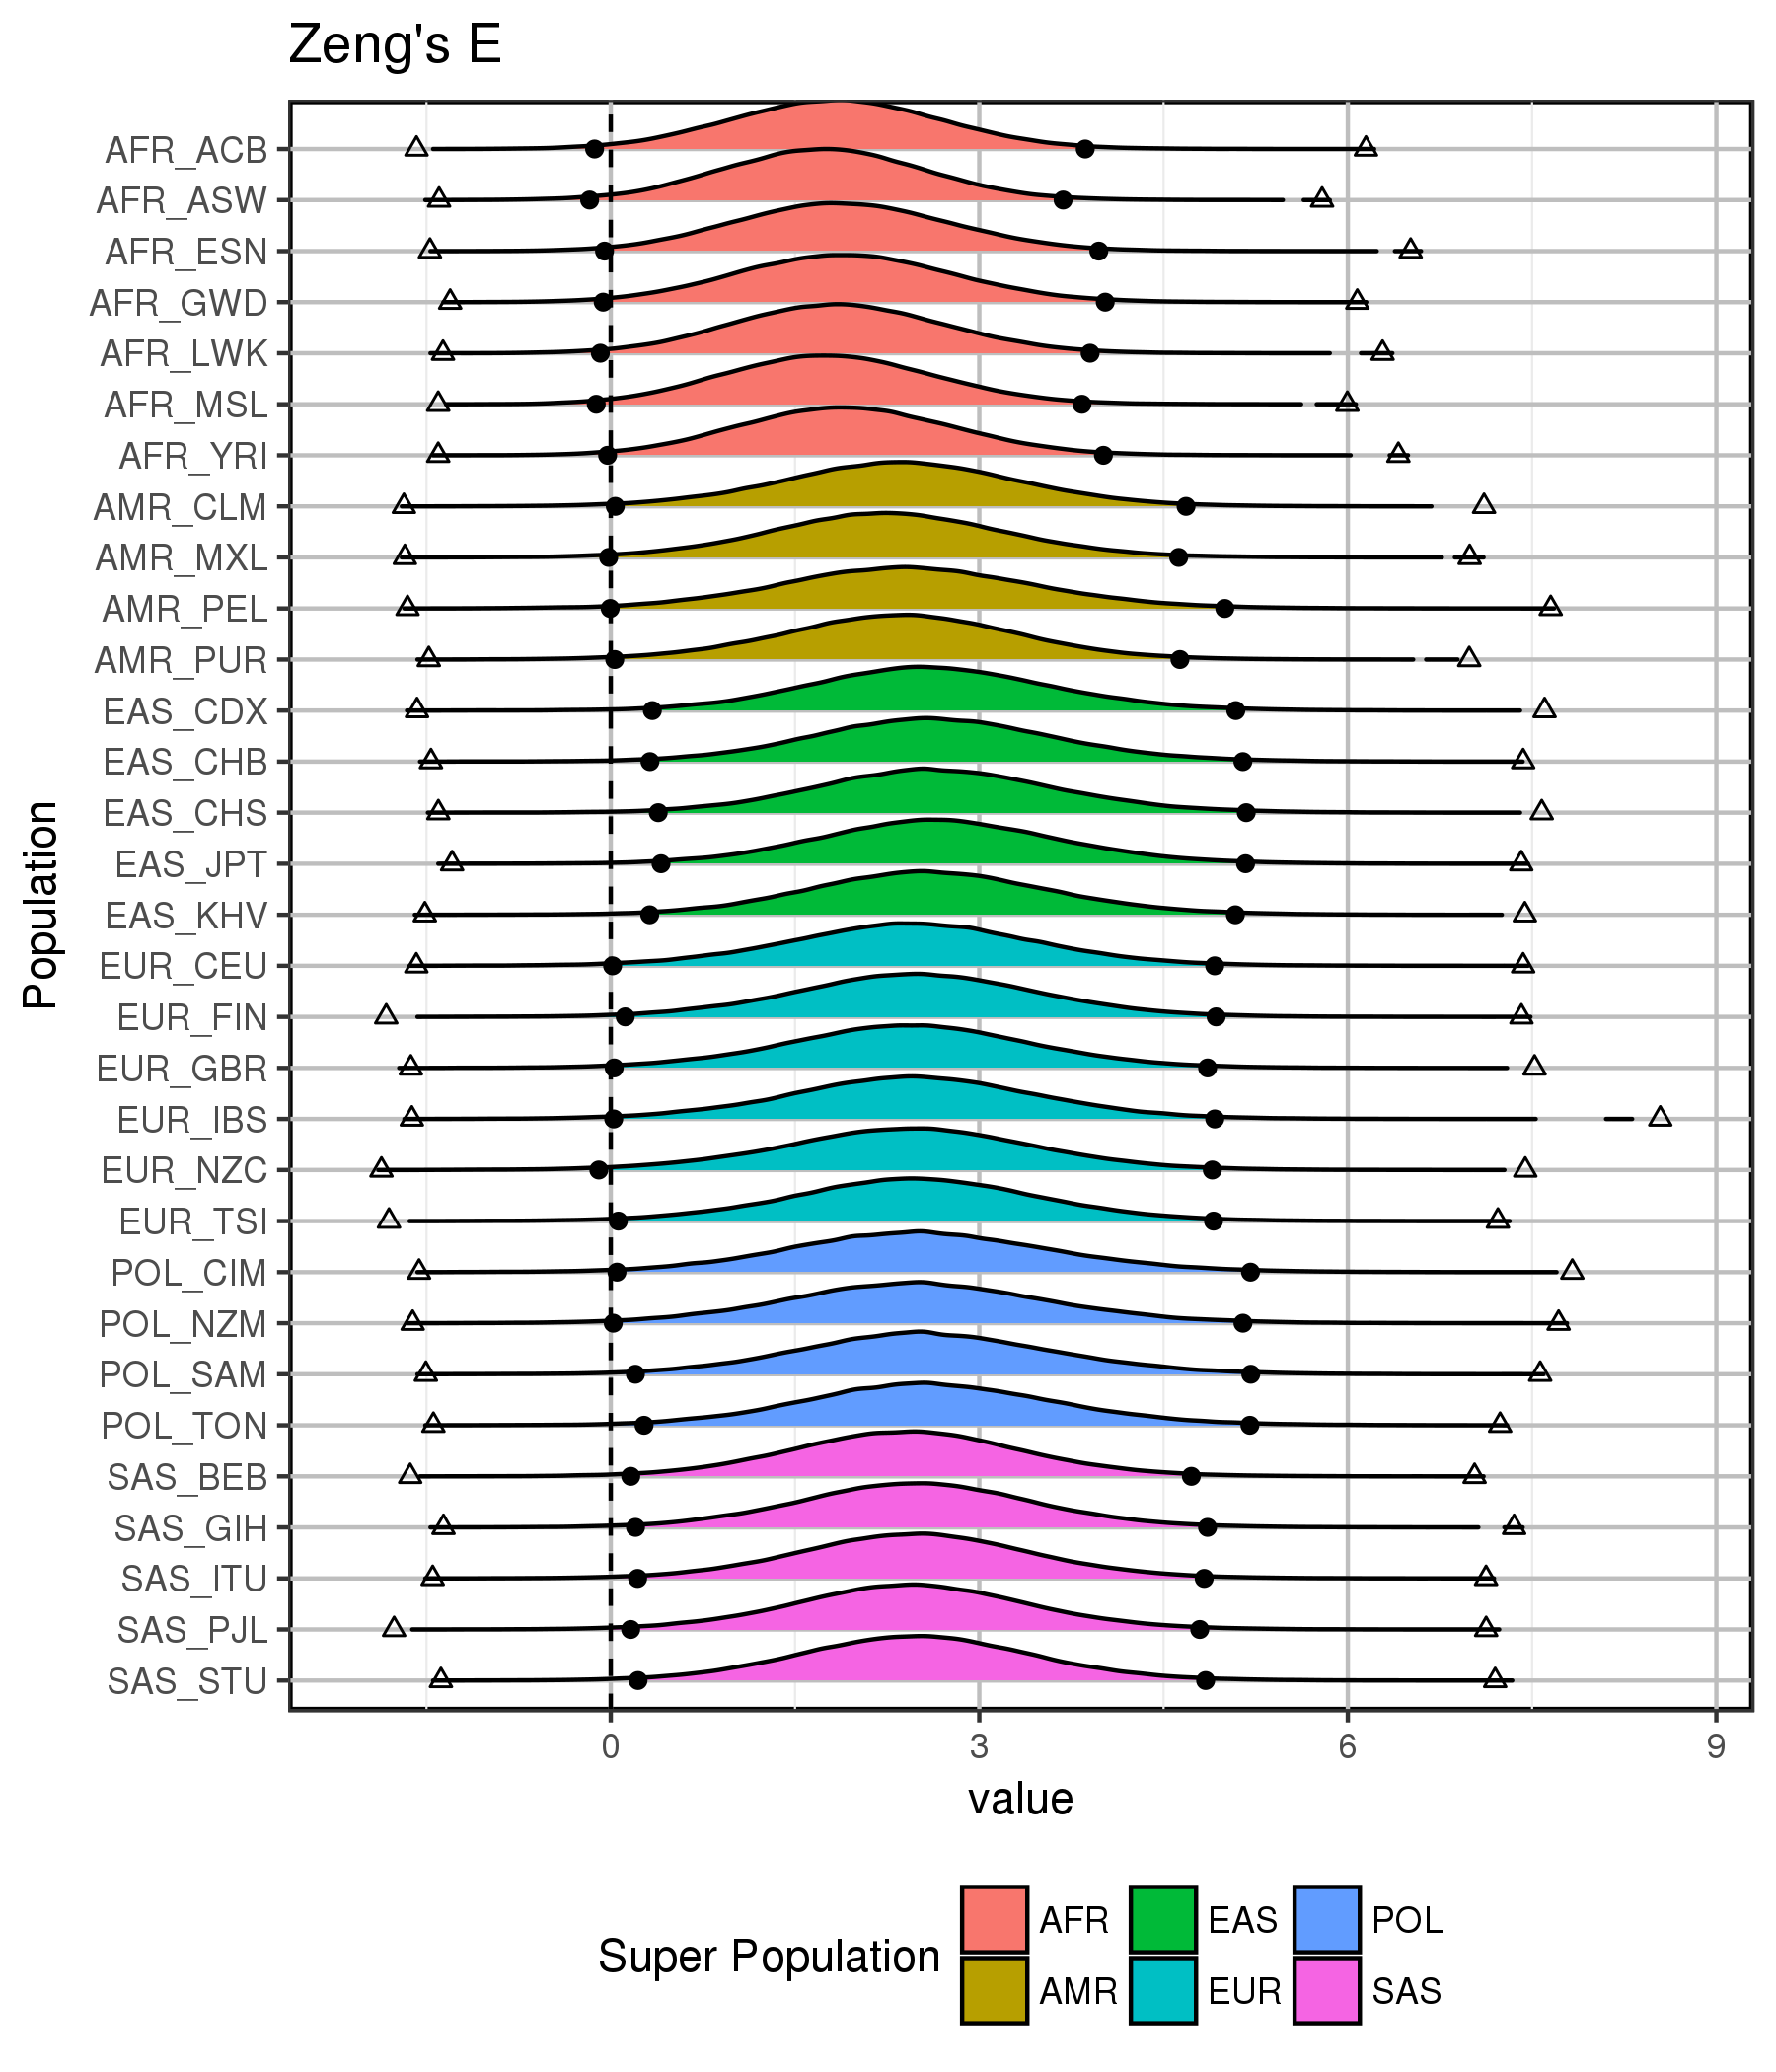
\includegraphics{_bookdown_files/images/04_clustering/ze_densities} \caption[Plot of the distribution of \gls{ze} by population.]{Plot of the distribution of \gls{ze} by population.
Triangles indicate the minimum and maximum values. Dots indicate the
1\textsuperscript{st} and 99\textsuperscript{th} percentiles for each
population.}\label{fig:zeDensity}
\end{figure}

\begin{table}

\caption{\label{tab:unnamed-chunk-25}\label{tab:superGlobalSummaryZE} Summary statistics for \gls{ze} by super population.}
\centering
\resizebox{\linewidth}{!}{
\begin{tabular}[t]{lrrrrrrr}
\toprule
Super Population & Mean & SD & Min & 1st Percentile & Median & 99th Percentile & Max\\
\midrule
AFR & 1.850 & 0.860 & -1.581 & -0.096 & 1.838 & 3.910 & 6.511\\
AMR & 2.346 & 0.994 & -1.684 & 0.012 & 2.340 & 4.754 & 7.652\\
EAS & 2.642 & 1.001 & -1.577 & 0.352 & 2.620 & 5.135 & 7.602\\
EUR & 2.452 & 1.024 & -1.866 & 0.024 & 2.453 & 4.904 & 8.544\\
POL & 2.559 & 1.065 & -1.613 & 0.122 & 2.535 & 5.194 & 7.827\\
SAS & 2.463 & 0.968 & -1.763 & 0.192 & 2.458 & 4.812 & 7.354\\
\bottomrule
\end{tabular}}
\end{table}











\begin{figure}
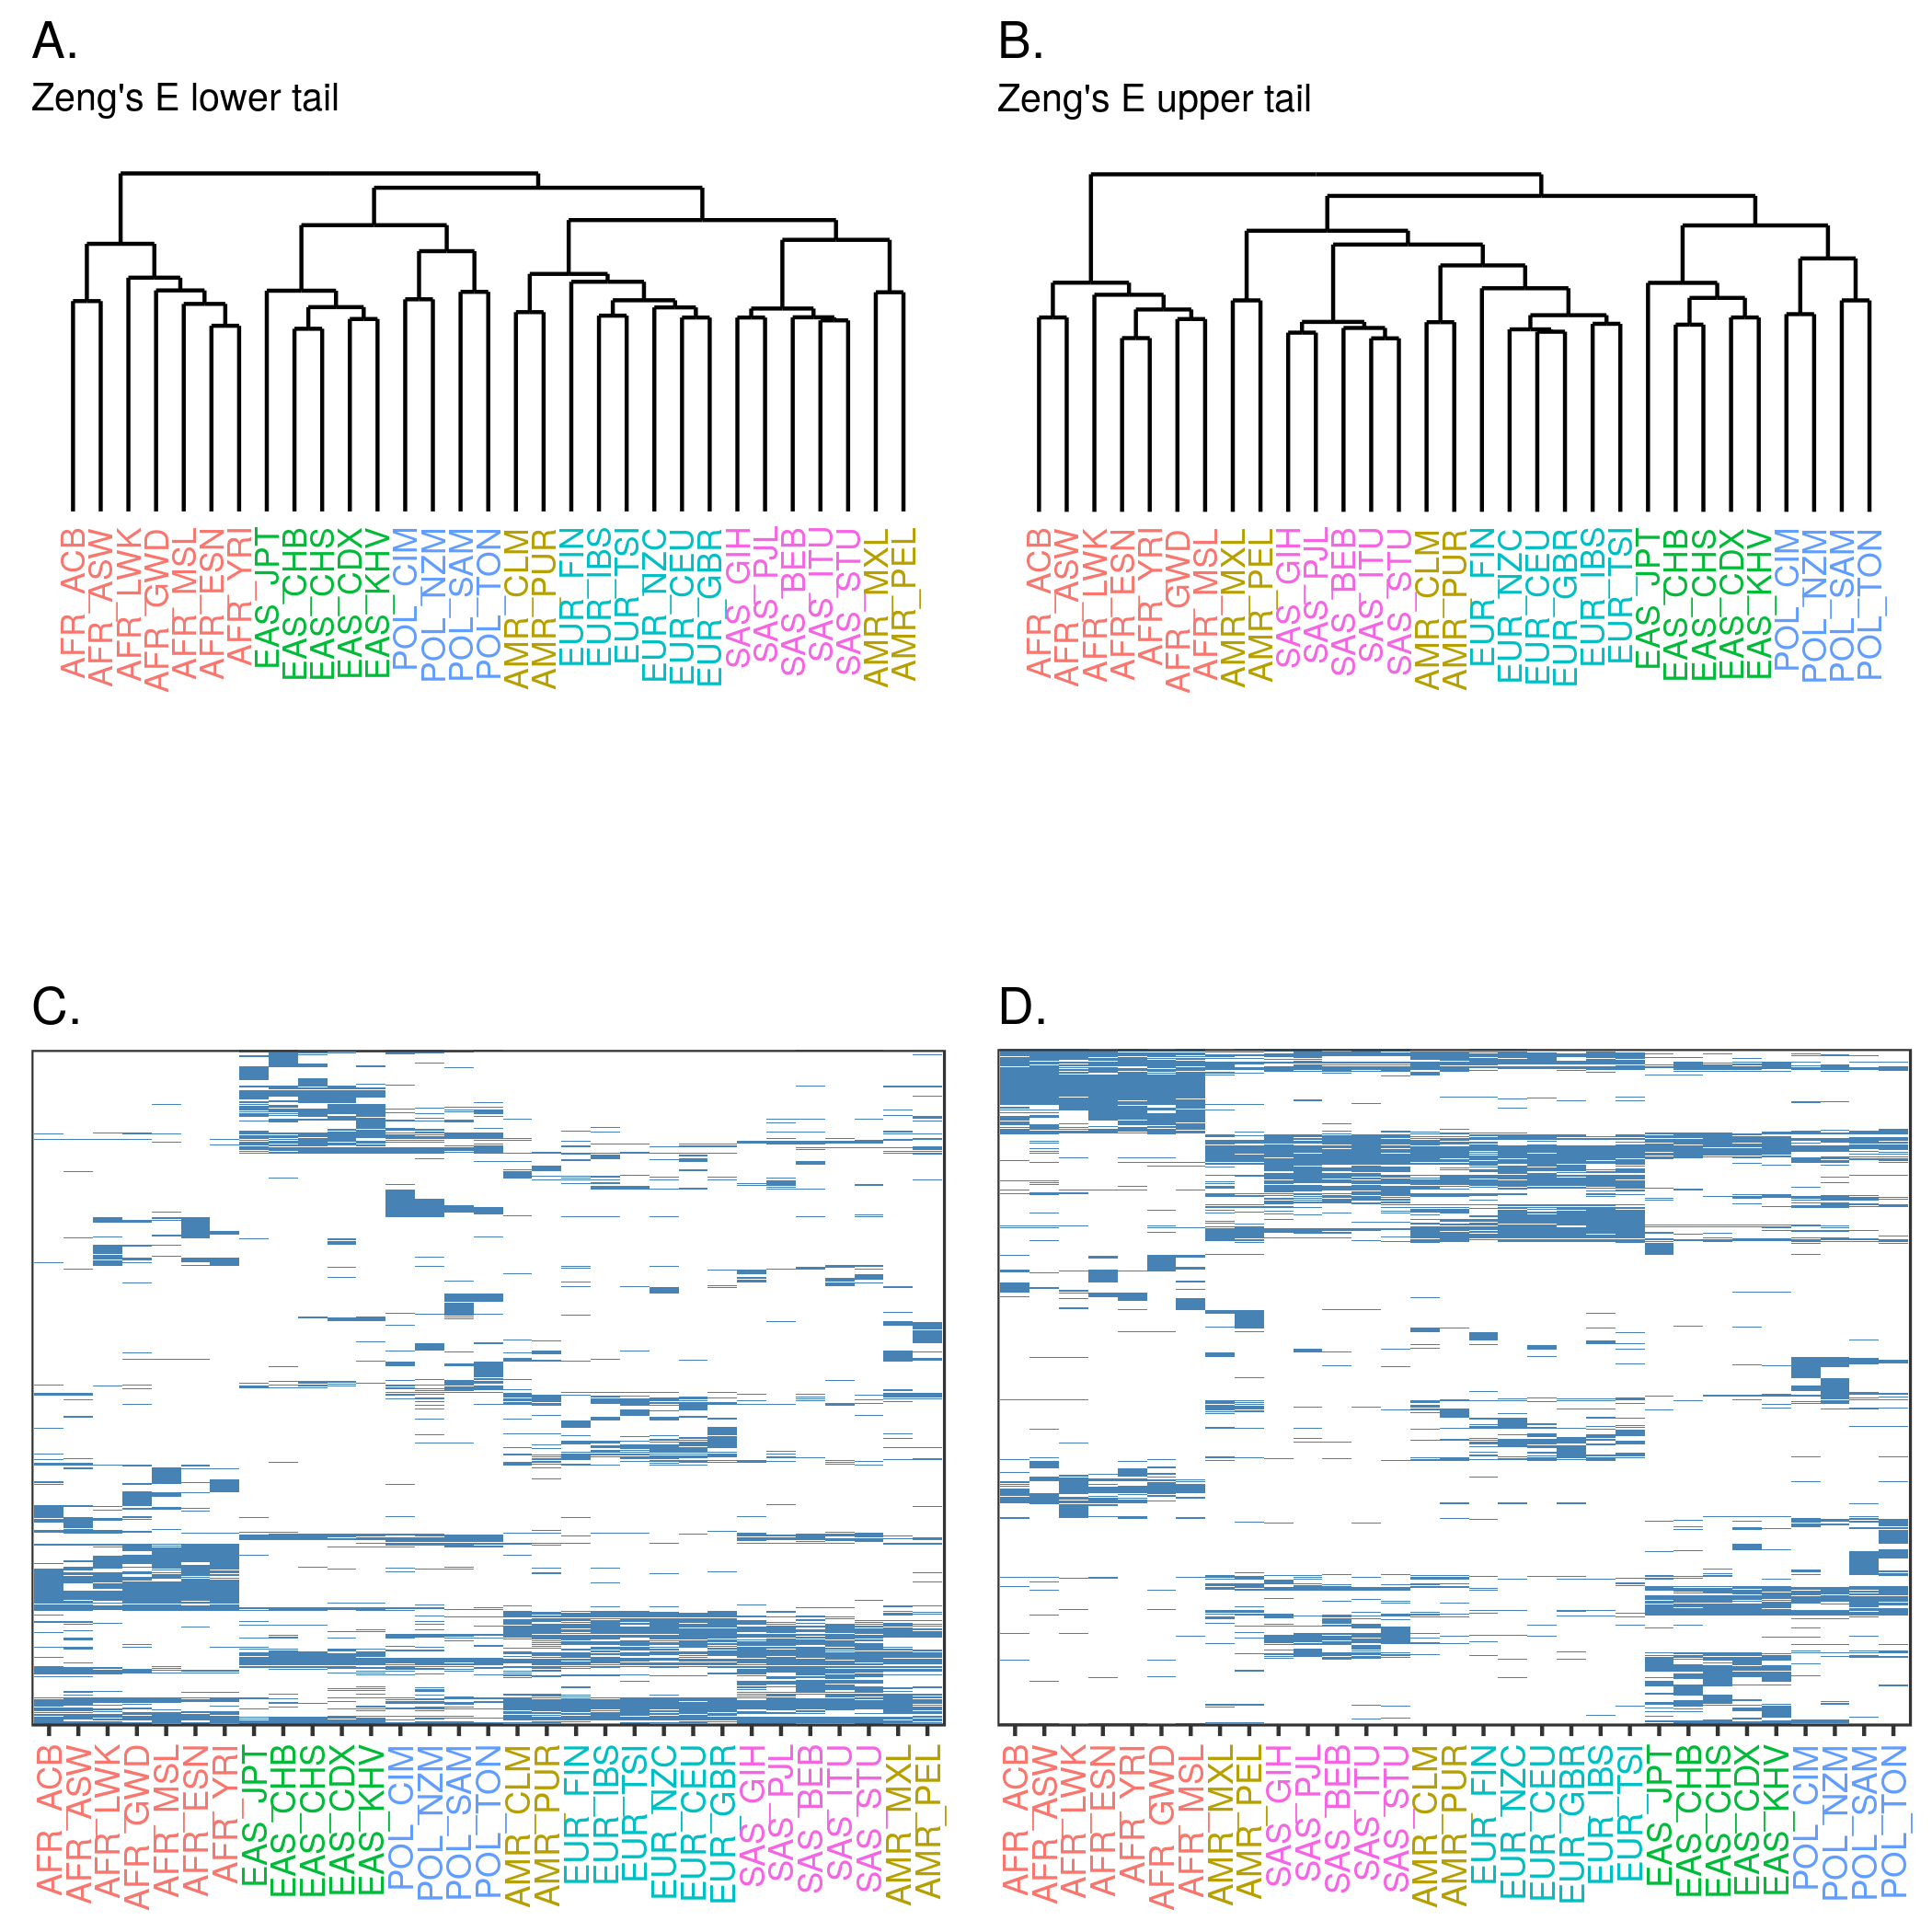
\includegraphics[width=6in,]{images/04_clustering/zeTop1000} \caption[Hierarchical clustering of \gls{ze} using the upper and lower 1\% of the distribution.]{Hierarchical clustering of \gls{ze} using the upper and
lower 1\% of the distribution. \textbf{A} and \textbf{B} Dendrograms
representing the clusters of \gls{ze} lower and upper tails
respectively, using hierarchical clustering with Euclidean distance and
complete linkage, and coloured by super population. \textbf{C} and
\textbf{D} Plots representing the windows present in each population
from the lower and upper tails respectively. A blue line represents
presence of a window, white represents the absence of a window in the
1\% of the distribution for a population.}\label{fig:zeTop1000}
\end{figure}

\Gls{ze} for both extremes of the distribution (Figure
\ref{fig:zeTop1000}), clustered all populations except \gls{amr} into
their respective super populations. The \gls{amr} population was split
into \gls{clm} and \gls{pur} which was grouped with the \gls{eur}
populations, and \gls{mxl} and \gls{pel} which were grouped as a
separate exclusive cluster. The groupings of all super populations was
the same for both tails, however, in the dendrogram the difference comes
from where the \gls{amr} populations were relative to the other super
populations with the \gls{mxl} and \gls{pur} populations changing
slightly in how close to the \gls{sas} group they were. Exclusivity of
clusters was high with only the \gls{amr} -\gls{eur} group not being
exclusive to a single super population.

\paragraph{\texorpdfstring{Clustering Zeng's \emph{E}
1\textsuperscript{st}
percentile}{Clustering Zeng's E 1st percentile}}\label{clustering-zengs-e-1st-percentile}

There were a total of 14,052 windows, with 1371 windows specific to
Polynesian populations in the lower tail. This compared to 3002 windows
for \gls{afr}, 605 windows for \gls{amr}, 976 windows for \gls{eur}, and
1149 windows for \gls{eas}. There were a total of 444 windows specific
to the Eastern Polynesian populations, with 191 specific to \gls{cim}
and 130 specific to \gls{nzm}. The Western Polynesian populations had
618 unique windows, 204 were unique to \gls{sam} and 250 unique to
\gls{ton}. The mean number of unique windows was 119.5 (SD 64.1) in the
lower tail. There were 36 genes that intersected windows that were only
in the four Polynesian populations and no other populations (Table
\ref{tab:polZeNegGenes}). None of these genes were associated with urate
or co-morbidities.

\paragraph{\texorpdfstring{Clustering Zeng's \emph{E}
99\textsuperscript{th}
percentile}{Clustering Zeng's E 99th percentile}}\label{clustering-zengs-e-99th-percentile}

In the upper tail there were a total of 13,684 windows with 1320 windows
specific to Polynesian populations. This compared to 2909 windows for
\gls{afr}, 584 windows for \gls{amr}, 900 windows for \gls{eur}, and
1200 windows for \gls{eas}. The Eastern Polynesian populations had 467
unique windows, the \gls{cim} had211 unique windows, and \gls{nzm} had
141 unique windows. The Western Polynesian populations had 594 unique
windows. Of those, 204 were unique to \gls{sam} and 264 unique to
\gls{ton}. The mean number of unique windows per population was 113.5
(SD 64.3)

\paragraph{\texorpdfstring{Metabolic associated diseases in the extremes
of Zeng's
\emph{E}}{Metabolic associated diseases in the extremes of Zeng's E}}\label{metabolic-associated-diseases-in-the-extremes-of-zengs-e}

There were 34 genes that were in the list of genes of metabolic disease
associated genes and also had windows in the 1\textsuperscript{st}
percentile, that intersected them from the Polynesian populations. Some
examples of these genes are \emph{MACF1}, \emph{AGBL4}, \emph{DACH1},
and \emph{RBMS1}. \emph{MACF1} had windows that were in the
1\textsuperscript{st} percentile of all populations. \emph{AGBL4} and
\emph{DACH1} had windows in nearly every population except for most
\gls{afr} populations. \emph{RBMS1} was only in the
1\textsuperscript{st} percentile for the Western Polynesian populations
\gls{sam} and \gls{ton}. Windows of the 99\textsuperscript{th}
percentile in the Polynesian populations that intersected the metabolic
disease associated genes tended to also be found in the populations of
\gls{eas}, and many also were in common with all other populations but
not many were in common with the \gls{afr} populations. There were 37
genes that were in the 99\textsuperscript{th} percentile for
Polynesians. Some examples were \emph{CHST8}, \emph{ERBB4}, \emph{FHIT},
\emph{PTPRD}, and \emph{HMGA2}. \emph{CHST8} had windows that were in
the 99\textsuperscript{th} percentile for the four Polynesian
populations, as well as the populations of \gls{eas} with a couple of
populations of both \gls{sas} and \gls{eur} too. \emph{ERBB4} had
windows that were in both \gls{pol} and \gls{eas} populations.
\emph{FHIT} had windows for the Western Polynesian populations,
\gls{sam} and \gls{ton} and most of the populations from \gls{eas} and
\gls{sas}. \emph{PTPRD} had windows from the Eastern Polynesian
populations of \gls{cim} and \gls{nzm}, these windows were also in
common with populations mostly from \gls{eur}, while some other windows
were in common with the Eastern Polynesian populations and \gls{afr}.
\emph{HMGA2} had windows in all of the super populations except
\gls{afr}.

\subsubsection{Summary of clustering on extremes
regions}\label{summary-of-clustering-on-extremes-regions}

Clustering of the windows using that fell in the lower 1\% and upper
99\% of the distributions for grouped the populations of the \gls{pol}
super population together in all instances except the lower tail of
\gls{flf}. There were no windows that were present for a single
population in the 1\textsuperscript{st} percentile for all
frequency-based statistics. The same applied for the
99\textsuperscript{th} percentile. Pooling the windows for each
population within a super population for the 1st percentile, across all
intra-population frequency-based statistics used, had 16 genes. The
\gls{afr} superpopulation had \emph{PHF7}; \gls{eas} had \emph{ALMS1},
\emph{OPLAH}, \emph{EXOSC4}, \emph{GPAA1}, \emph{CYC1}, and
\emph{SHARPIN}; \gls{eur} had \emph{NTN3}; \gls{pol} had \emph{FANCM}
and \emph{ALMS1}; and \gls{sas} had \emph{ABHD14A}, \emph{ACY1},
\emph{ABHD14B}, \emph{TBC1D24}, and \emph{NTN3}. \gls{eas} and \gls{pol}
had \emph{ALMS1}, a kidney function-associated locus
\citep{pattaro2016genetic} in common, and \gls{eur} and \gls{sas} had
\emph{NTN3} in common. There were no windows in the
99\textsuperscript{th} percentile that when populations were pooled as
super populations were present in all four frequency-based statistics.

\FloatBarrier

\subsection{Hierarchical clustering of selected haplotypic
regions}\label{hierarchical-clustering-of-selected-haplotypic-regions}

A similar approach as with clustering of the frequency spectrum-based
statistics was used to investigate similarities in regions that had
evidence of possible selection in the intra-population haplotypic based
selection methods. To do this, the significant \gls{ihs} or \gls{nsl}
results were clustered into regions (Table \ref{tab:hapclustab}), and
the percentage of bases overlapping between populations was calculated
in these regions. The proportion of shared regions, based on region
overlap, was used to cluster populations, given the total region that
was significant for a single population. This was to investigate if
there was a commonality between populations in the haplotypic regions
that had evidence for selection, the hypothesis being that populations
in similar geographic regions would have had a similar environmental
exposure, and therefore have similar regions of the genome under
selective pressure. Another possibility was that the selective pressure
was in a shared ancestral population.

Clustering on the proportion of shared regions (see section
\ref{haplocluster}) for both \gls{ihs} (Figure \ref{fig:ihsclust}) and
\gls{nsl} (Figure \ref{fig:nslclust}) grouped the individual populations
into their super populations, with the exception of the \gls{amr}
populations which were split into two separate groups. The order of
populations differed due to each population having a different total for
the size of region that was significant. Both \gls{ihs} and \gls{nsl}
gave similar groupings and had similar proportions of selected regions
shared.

\subsubsection{\texorpdfstring{\gls{ihs}}{}}\label{section}

For the \gls{ihs} significant regions, the populations with the least
regions shared between them were \gls{cim} and \gls{clm}, with 3.0\%
shared. The populations that had the largest proportion of region shared
was \gls{nzc} and \gls{ceu} with 56.7\% shared. Looking specifically at
the proportion of regions shared between Polynesian populations, for the
Eastern Polynesian populations there was \gls{nzm} with 34.5\% of
regions shared with \gls{cim}, and \gls{cim} shared 35.6\% of regions
with \gls{nzm}. In the Western Polynesian populations, \gls{sam} shared
43.8\% of regions with \gls{ton}, but \gls{ton} shared 45.3\% of regions
with \gls{sam}. Out of all the significant \gls{ihs} regions for
Polynesian populations, only 1.7\% were in common across all Polynesian
populations. The Eastern Polynesians accounted for 59.9\% of the regions
from all of the Polynesian populations while the Western Polynesian
populations made up 50.1\%.

The proportion of significant \gls{ihs} regions the Polynesian
populations shared with AMR was 14.5\%, AFR was 14.5\%, EAS was 12.9\%,
EUR was 10.4\%, and SAS was 9.6\%. This was lower than the mean (20.3\%)
for proportion of regions shared between the other super populations.
The Polynesian populations were clustered together with a high
proportion of shared significant regions. The Eastern Polynesians had on
average 35.0\% in common, and the Western Polynesian populations had
44.6\%. However, shared regions between the Eastern and Western
Polynesian populations was 14.2\% on average. Of the clustered regions
of significant \gls{ihs} that were in common between all of the
\gls{pol} populations, 70 genes intersected the regions. These genes
were part of 57 pathways in the \gls{kegg} 2016 pathways in Enrichr, but
none were significantly enriched. Regions that were in common between
\gls{nzm} and \gls{cim} had 392 genes that intersected, and were
involved with 174 pathways. Again, no pathways were significantly
enriched. For the regions that were in common between \gls{sam} and
\gls{ton}, there were 502 genes that intersected the regions. They
belonged to 223 pathways, with only a single pathway significantly
enriched (Benjamini-Hochberg adjusted P = 0.023) with seven of 44 genes
(\emph{ABCA5}, \emph{ABCC8}, \emph{ABCC5}, \emph{TAP2}, \emph{ABCA9},
\emph{ABCB8}, and \emph{ABCA8}). That pathway was ``ABC
transporters\_Homo sapiens\_hsa02010''.

\begin{figure}
\includegraphics{_bookdown_files/04-Clustering_files/figure-latex/ihsclust-1} \caption[Hierarchical clustering of \acrshort{ihs}.]{\gls{ihs} Clustering: A. Dendrogram from hierarchical
clustering based on proportion of significant \gls{ihs} regions shared
between populations, coloured by super population. B. Heatmap showing
the proportion of significant \gls{ihs} regions shared. The population
listed on the axis is used as A in the calculation = (A \(\cap\) B)/ A.
Axes have been ordered according to the hierarchical clustering.}\label{fig:ihsclust}
\end{figure}








\subsubsection{\texorpdfstring{\gls{nsl}}{}}\label{section-1}

The clustering results using regions of significant \gls{nsl} gave the
same groupings as \gls{ihs} (Figure \ref{fig:nslclust}). This similarity
was also seen with the differences in individual populations, where
\gls{nzc} and \gls{gbr} had the highest percentage of shared regions at
59.9\%. \Gls{nzm} and \gls{beb} shared the lowest percentage of regions
at 0.5\%. The percentage of the significant \gls{nsl} regions the
Polynesian populations shared with AMR was 10.0\%, AFR was 10.4\%, EAS
was 11.6\%, EUR was 7.6\%, and SAS was 7.0\%. This was lower than the
mean (16.5\%) proportion of region sharing between super populations.
The Polynesian populations were clustered together with a high
proportion of shared significant regions. The Eastern Polynesians had on
average 36.5\% in common. NZM shared 38.3\% of regions with CIM, whereas
CIM shared 34.6\% of regions with NZM. The Western Polynesians had
40.4\% of regions shared on average. SAM shared 39.1\% of regions with
TON, but TON shared 41.8\% of regions with SAM. However, between the
Eastern and Western populations, region sharing averaged 11.2\%. Of the
regions from all of the Polynesian populations, the Western Polynesian
populations made up 56.7\%. The Eastern Polynesians made up 51.0\%. The
total percentage of regions common for all Polynesian populations was
1.4\%. This shows that within the Eastern or Western Polynesian groups
there was a larger proportion of regions that were similar for
significant \gls{nsl}, than between the Eastern and Western groups.

The regions that were in common for significant \gls{nsl} between all of
the \gls{pol} populations intersected 27 genes. These genes were part of
10 pathways, but none were significantly enriched. Regions that were in
common between \gls{nzm} and \gls{cim} had 230 genes that intersected,
and were involved with 160 pathways. A single pathway,
``Glycosaminoglycan degradation\_Homo sapiens\_hsa00531'', was
significantly enriched (adjusted P 9.223 x 10\textsuperscript{-3}) with
four of 19 genes (\emph{HPSE2}, \emph{HYAL1}, \emph{HYAL2}, and
\emph{HYAL3}). The regions that were in common between \gls{sam} and
\gls{ton} intersected 319 genes. There were 197 pathways that these
genes were part of but none were significantly enriched.

\begin{figure}
\includegraphics{_bookdown_files/04-Clustering_files/figure-latex/nslclust-1} \caption[Hierarchical clustering of \acrshort{nsl}.]{\gls{nsl} Clustering: A. Dendrogram from hierarchical
clustering based on proportion of significant \gls{nsl} regions shared
between populations, coloured by super population. B. Heatmap showing
the proportion of significant \gls{nsl} regions shared. The population
listed on the axis is used as A in the calculation = (A \(\cap\) B)/ A.
Axes have been ordered according to the hierarchical clustering.}\label{fig:nslclust}
\end{figure}








\subsubsection{Metabolic disease associated
genes}\label{metabolic-disease-associated-genes}

In the clustered-significant regions of both \gls{ihs} and \gls{nsl}
(Table \ref{tab:hapclustab}) there were 405 independent regions that
overlapped with genes associated with urate and metabolic diseases from
all populations, for Polynesian populations the number of regions was
104. \gls{ihs} had 337 regions, while \gls{nsl} had 329, and in common
between the two statistics were 261 regions. The regions of the
Polynesian populations covered 433 \glspl{snp} for \gls{ihs} and 301 for
\gls{nsl}, with 149 in common between them. For the genes that had
significant regions in Polynesian populations, 8 regions intersected
genes that had been associated with urate and gout, 67 with obesity, 30
with \gls{t2d}, 6 with kidney disease, and 5 with metabolic syndrome.

Using the significant \glspl{snp} for these \gls{ihs} and \gls{nsl} (as
in Chapter 3) there were a total of 204 \glspl{snp} that were
significant in a Polynesian population and also significant in at least
one other population for \gls{ihs}, and 93 for \gls{nsl} (Table
\ref{tab:ihsnslPolGenes}). The number of \glspl{snp} that were
significant in both \gls{ihs} and \gls{nsl} in the Polynesian population
was 48.

The urate associated gene \emph{ABCG2} had a single \gls{snp}
(rs2622626) that was significant in \gls{ton} that was in common for
significance for \gls{ihs} in two other populations, \gls{gih} and
\gls{itu}, both were from the \gls{sas} super population. The situation
was the same for \gls{nsl}, but with the addition of \gls{jpt}.

The \gls{sam} and \gls{ton} populations had multiple \glspl{snp} in
common that were significant for both \gls{ihs} and \gls{nsl}. An
example is in \emph{LRP1B}, where there were three \glspl{snp}:
rs10173806, rs4591293, and rs2890615. Rs2890615 was also significant in
\gls{esn} and \gls{chs}.

\emph{ERBB4} had a single significant \gls{snp}, rs6707285, in
\gls{sam}, and was also significant in \gls{pur}, \gls{khv}, \gls{ibs},
\gls{tsi}, and \gls{gbr}. \emph{FHIT} also had a single significant
\gls{snp}, but this was in the \gls{nzm}, \gls{chb}, \gls{chs},
\gls{cdx}, \gls{khv}, and \gls{pel} populations. Of the metabolic
disease genes, \emph{ERBB4} and \emph{FHIT} were also found by
\citet{pickrell2009signals} in the Human Genome Diversity-CEPH Panel
using \gls{ihs} and \gls{xpehh}.

One of the main regions, chr20:33470694-34556005, had 11 significant
\glspl{snp} in Polynesian populations as well as up to 16 other
populations, contained the obesity-associated gene \emph{GDF5} and the
neighbouring genes \emph{CEP250} and \emph{UQCC1.} The majority of the
significant \glspl{snp} were for the ancestral allele. Both rs1570841
and rs4911502 were significant in the populations of \gls{amr}
(\gls{clm}, \gls{mxl} and \gls{pur}), \gls{eas} (\gls{cdx}, \gls{chb},
\gls{chs}, \gls{jpt}, and \gls{khv}), \gls{eur} (\gls{ceu}, \gls{fin},
\gls{gbr}, \gls{ibs}), \gls{pol} (\gls{cim}, \gls{nzm}, and \gls{ton}),
and \gls{sas} (\gls{beb} and \gls{itu}. Both \glspl{snp} were for the
ancestral allele. Four \glspl{snp}, rs4911178, rs4911494, rs6087704, and
rs6087704, intersected both \emph{GDF5} and \emph{UQCC1}, and were
significant for the derived alleles in the \gls{cim} and \gls{jpt}
populations.

\subsection{Disease-associated gene clustering}\label{genelistcluster}

To assess if there was specificity of selection for the metabolic
disease gene lists or if the population groupings could be obtained from
any list of genes, clustering was performed using the actual statistic
values for the genes. These values were median-centred to account for
the population specific shifting of distributions which would have
accounted for the majority of difference in the distance calculation.
Gene lists were chosen for metabolic-related disease and compared to
lists of random genes (section \ref{randomgenes}) to assess clustering
specificity to metabolic disease.

\subsubsection{Clustering of median-centred window values for urate and
gout-associated
genes}\label{clustering-of-median-centred-window-values-for-urate-and-gout-associated-genes}

There were 62 loci that had an association with urate or gout at a
genome-wide significance level in the \gls{gwas} catalog. This mapped to
435 windows for each of the frequency-based selection test statistics.
Tables \ref{tab:gouttdgeneclus}, \ref{tab:goutfwhgeneclus},
\ref{tab:goutflfgeneclus}, and \ref{tab:goutzegeneclus} contain the
median centred values for the windows used in the clustering. All
statistics (\gls{td}, \gls{fwh}, \gls{flf}, and \gls{ze}) grouped most
of the super populations correctly and nearly all clusters had good
exclusivity for each single super population (Tables
\ref{tab:proportion} and \ref{tab:exclusivity}). \Gls{td}, \gls{fwh},
and \gls{ze} also had an Eastern/Western Polynesian population sub group
within the Polynesian group (Figure \ref{fig:goutdendros}). Unlike the
F\textsubscript{ST} clustering, the \gls{amr} populations were grouped
together for \gls{td}, \gls{fwh}, and \gls{ze}. The \gls{eas} and
\gls{pol} populations were closest for \gls{td}, \gls{flf}, \gls{fwh},
and \gls{ze}.

One of the trends across all of the statistics, was that within a super
population, the range of values within a gene were very similar, but
between super populations there could be completely different
directions. There was also variation between loci, in terms of which
populations had overall more positive or negative windows. \emph{INHBB}
was an example of a locus with \gls{fwh} that showed similarity in
scores of populations with similar ancestry, such as between the
\gls{pol} and \gls{eas} which were positive, \gls{sas} was near zero but
slightly positive, \gls{eur} and \gls{amr} were near zero but slightly
negative, and \gls{afr} was more negative (Table
\ref{tab:goutfwhgeneclus}). Another example was \emph{RREB1}, where for
\gls{td}, the \gls{pol} populations were sitting around -2 , with the
\gls{eas} populations slightly less negative, and the other populations
having windows that were around zero (Table \ref{tab:gouttdgeneclus}). A
similar pattern was seen in \emph{RREB1} with \gls{flf} (Table
\ref{tab:goutflfgeneclus}). With \gls{ze}, \emph{SLC22A12} and
\emph{SLC22A12} both had \gls{afr}, \gls{eas}, and \gls{pol} negative,
and \gls{amr}, \gls{eur}, and \gls{sas} positive (Table
\ref{tab:goutzegeneclus}). And both \emph{SLC17A1} and \emph{SLC17A4}
had all populations with negative \gls{ze}, except the \gls{pol}
populations, which were positive. \emph{SLC2A9} tended to be overall
more negative in value for all statistics for both \gls{pol} and
\gls{eas} than for the other super populations.





\begin{figure}
\includegraphics{_bookdown_files/04-Clustering_files/figure-latex/goutdendros-1} \caption[Dendrograms created from hierarchical clustering applied to windows from loci associated with urate and gout]{Dendrograms created from hierarchical clustering
applied to windows from the 62 loci associated with urate and gout.
Coloured by super population.}\label{fig:goutdendros}
\end{figure}

\subsubsection{Clustering of median-centred window values for
obesity-associated
genes}\label{clustering-of-median-centred-window-values-for-obesity-associated-genes}

The \gls{gwas} catalog had 269 loci associated with obesity, this was
represented by 4099 windows and the clustering resulted in the groupings
of super populations (Figure \ref{fig:obesitydendros}). Exclusivity of a
single super population to a cluster was also high with the notable
exception being the \gls{amr} populations of \gls{clm} and \gls{pur}
often being part of the \gls{eur} cluster (Tables \ref{tab:proportion}
and \ref{tab:exclusivity}). Tables \ref{tab:obesitytdgeneclus},
\ref{tab:obesityfwhgeneclus}, \ref{tab:obesityflfgeneclus}, and
\ref{tab:obesityzegeneclus} contain the median centred statistic values
for the windows used in the clustering. The Polynesian super population
cluster was also closest to \gls{eas} in all selection statistics and
also had an Eastern/Western sub-grouping within the \gls{pol} group.

Much like the urate-associated genes, the same trend of within a super
population, genes had similar values, but there could be completely
different directions of statistic between super populations held. Some
examples of this included \emph{LEPR} and \emph{FOXE1}, where for
\gls{fwh}, \gls{td}, and \gls{flf}, for the \gls{eas} and \gls{pol}
populations the windows were mostly negative, whereas for the other
populations they were close to zero or even positive. \emph{ARL15} was
an example of a locus that all populations had a range of values, but
the \gls{pol} populations was the negative most for all statistics, and
in \gls{td}, \gls{fwh}, and \gls{flf} the \gls{eas} populations showed
similarity with the \gls{pol} populations in the values of the
statistics in being overall quite negative.

\begin{figure}
\includegraphics{_bookdown_files/04-Clustering_files/figure-latex/obesitydendros-1} \caption[Dendrograms created from hierarchical clustering applied to windows from obesity-associated loci.]{Dendrograms created from hierarchical clustering
applied to windows from the 269 loci associated with obesity. Coloured
by super population.}\label{fig:obesitydendros}
\end{figure}





\subsubsection{Clustering of median-centred window values for type 2
diabetes-associated
genes}\label{clustering-of-median-centred-window-values-for-type-2-diabetes-associated-genes}

The \gls{gwas} catalog had 99 genes associated with \gls{t2d}. These
were represented by 1471 windows and clustering of the \gls{t2d}
associated genes grouped the individual populations into their super
population groups. For all clustering the \gls{amr} populations were
split, with \gls{clm} and \gls{pur} grouped with the \gls{eur}
populations for \gls{td}, \gls{fwh}, and \gls{ze} (Figure
\ref{fig:t2ddendros}). Tables \ref{tab:t2dtdgeneclus},
\ref{tab:t2dfwhgeneclus}, \ref{tab:t2dflfgeneclus}, and
\ref{tab:t2dzegeneclus} contain the median centred statistic values for
the windows used in the clustering. The \gls{pol} populations were
assigned two exclusive groups through the cutree method that created an
Eastern/Western Polynesian split for \gls{td}, \gls{fwh}, \gls{flf}, and
\gls{ze}. \gls{fwh} and \gls{ze} had a similar pattern to the groupings
of the whole chromosome F\textsubscript{ST} clustering.

Again, most of the loci that were associated with \gls{t2d} followed the
same trend of values within a super population being similar, and
differences between the super populations. An example where this was not
the case was \emph{SSR1}, where all populations, except the Eastern
Polynesian populations were very similar and close to zero, whereas the
Eastern Polynesian populations were negative in all statistics, but not
extreme enough to be in the 1\textsuperscript{st} percentile.





\begin{figure}
\includegraphics{_bookdown_files/04-Clustering_files/figure-latex/t2ddendros-1} \caption[Dendrograms created from hierarchical clustering applied to windows from \gls{t2d}-associated loci.]{Dendrograms created from hierarchical clustering
applied to windows from the 99 loci associated with \gls{t2d}. Coloured
by super population.}\label{fig:t2ddendros}
\end{figure}

\subsubsection{Clustering of median-centred window values for kidney
disease-associated
genes}\label{clustering-of-median-centred-window-values-for-kidney-disease-associated-genes}





\begin{figure}
\includegraphics{_bookdown_files/04-Clustering_files/figure-latex/kidneydendros-1} \caption[Dendrograms created from hierarchical clustering applied to windows from kidney disease-associated loci.]{Dendrograms created from hierarchical clustering
applied to windows from the 53 loci associated with kidney disease.
Coloured by super population.}\label{fig:kidneydendros}
\end{figure}

The GWAS catalog had 53 genes associated with kidney disease, this was
represented by 390 windows. The clustering of the kidney
disease-associated genes grouped the individual populations into their
super population groups for \gls{afr} and \gls{sas} using \gls{td},
\gls{fwh}, \gls{flf}, and \gls{ze}. Populations from \gls{pol} and
\gls{eas} were clustered into separate clusters with \gls{td} and
\gls{flf} but were clustered together for \gls{fwh} and \gls{ze} (Figure
\ref{fig:kidneydendros}). Tables \ref{tab:kdtdgeneclus},
\ref{tab:kdfwhgeneclus}, \ref{tab:kdflfgeneclus}, and
\ref{tab:kdzegeneclus} contain the median centred statistic values for
the windows used in the clustering. \gls{td} clustered populations from
\gls{afr}, \gls{eas}, \gls{pol}, and \gls{sas} into super population
specific and exclusive clusters.

The same trend as for the other gene lists still stood with the kidney
disease gene list. Although for \gls{fwh} and \gls{ze} there was a
higher similarity between \gls{ton} and \gls{khv} than with the other
populations of their respective super populations. This was largely
driven by \emph{ALMS1}, where \gls{ton}, \gls{khv}, and the populations
of \gls{afr}, were negative, and the other populations were positive for
\gls{ze} and the opposite was the case for \gls{fwh}.

\subsubsection{Clustering of median-centred window values for metabolic
syndrome-associated
genes}\label{clustering-of-median-centred-window-values-for-metabolic-syndrome-associated-genes}





\begin{figure}
\includegraphics{_bookdown_files/04-Clustering_files/figure-latex/metsyndendros-1} \caption[Dendrograms created from hierarchical clustering applied to windows from metabolic syndrome-associated loci.]{Dendrograms created from hierarchical clustering
applied to windows from the 22 loci associated with metabolic syndrome.
Coloured by super population.}\label{fig:metsyndendros}
\end{figure}

The GWAS catalog had 22 genes associated with metabolic syndrome, this
was represented by 234 windows. The clustering of the metabolic syndrome
associated genes grouped individual populations into their super
population groups for \gls{td} and \gls{fwh} (Figure
\ref{fig:metsyndendros}). Tables \ref{tab:metsyntdgeneclus},
\ref{tab:metsynfwhgeneclus}, \ref{tab:metsynflfgeneclus}, and
\ref{tab:metsynzegeneclus} contain the median centred statistic values
for the windows used in the clustering. For \gls{flf}, the Polynesian
populations were assigned two exclusive clusters that followed the
Eastern/Western Polynesian split. \Gls{ze} clustered the individual
populations, except for \gls{pel}, into their super populations. The
Polynesian populations were grouped into entirely exclusive clusters for
all statistics. The same trends of within super populations having
similar statistic values and differences between super populations still
held in the gene list for metabolic syndrome.

\subsection{Random draws}\label{random-draws}

\subsubsection{Random windows}\label{random-windows}

It is possible that obtaining the population groupings by clustering the
most extreme windows for each statistic, could have occurred by chance.
To assess this, 10,000 iterations of random resampling of 2500 windows
per population was undertaken, and these windows were then clustered.
This was done so that the extreme tail clustering could be compared to
the random windows to see if the extreme window clustering performed
better in exclusivity and proportion of super population clustering than
by drawing windows at random. The maximum proportion of populations
being clustered into their designated super population was then
calculated when the tree was cut to have six groups (K = 6), one for
each super population. The mean proportion of populations grouped into
their super population was less than 0.5 for all super populations, with
an overall mean of 0.282 (Table \ref{tab:randtab}). This compared to a
mean proportion of 0.916 for the clustering of the extreme windows, this
implies that there is similarity in the regions of extreme score within
a super population, and differences in these regions between super
populations. Based on the results of the admixture analysis, K = 11 was
also tested and had higher mean exclusivity (0.424) than K = 6, due to
more possible individual clusters. The remainder of this section will
report on K = 6, as this reflects the number of super populations used
for the non-randomised data.

Not a single random draw grouped the all individual populations into all
of their respective super populations. Only the populations of the
\gls{afr} and \gls{eur} super populations did not each get fully grouped
into a cluster. Grouping at least 50\% of a super population was at best
12\% of the draws but for the larger super populations (\gls{afr},
\gls{eas}, \gls{eur}, and \gls{sas}) it was on average 4\% of the draws.
There were only eight random draws that had all super populations each
having half or more of their individual populations assigned to the same
group. The mean exclusivity of the random draws was low, ranging from
0.26 to 0.32 and there were no random draws in which the Polynesian
populations were all grouped together as a Polynesian exclusive cluster.

Compared to the clustering on the extreme tails, the random windows had
poorer exclusivity of clusters with a mean exclusivity of 28\%. The
populations were clustered into their super populations rarely for the
random windows and did not have multiple super populations being
clustered as the clustering of the extremes returned (Table
\ref{tab:randtab}). This indicates that there is a degree of similarity
of regions that are in the extremes of the distributions and the
populations who share them. This is largely due a minimum degree of
differences in similarity being needed in order for hierarchical
clustering to be effective for clustering. When windows are drawn at
random the differences, or distances, between populations is likely to
be equivalent, so the hierarchy is flatter, meaning small differences
have very large changes to the groupings.

\begin{table}

\caption{\label{tab:randtabpander}\label{tab:randtab} Proportion of individual populations assigned to their super population by hierarchical clustering across 10000 iterations of 2500 randomly drawn windows.}
\centering
\begin{threeparttable}
\begin{tabular}[t]{lrrrrrrlrrrrrrlrrrrrrlrrrrrrlrrrrrrlrrrrrrlrrrrrr}
\toprule
Super Population & Min & Mean & Std. Dev & Max & Prop50 (\%) & Total Complete (n)\\
\midrule
AFR & 0.286 & 0.389 & 0.103 & 0.857 & 2.1 & 0\\
AMR & 0.250 & 0.451 & 0.147 & 1.000 & 11.9 & 32\\
EAS & 0.200 & 0.429 & 0.118 & 1.000 & 3.6 & 6\\
EUR & 0.167 & 0.395 & 0.102 & 0.833 & 5.6 & 0\\
POL & 0.250 & 0.450 & 0.147 & 1.000 & 11.8 & 30\\
SAS & 0.200 & 0.423 & 0.116 & 1.000 & 3.3 & 2\\
\bottomrule
\end{tabular}
\begin{tablenotes}
\item Prop50 is the percentage of the iterations that had at least 50\% of each super population assigned the same cluster. Total complete is the number of iterations all populations of a super population were assigned the same cluster
\end{tablenotes}
\end{threeparttable}
\end{table}

\subsubsection{Random genes}\label{randomgenes}

In order to assess whether the clustering from gene lists was specific
to the disease associated genes used, lists of random genes were created
by selecting genes from a list containing all annotated genes, and then
clustered. Random gene lists were generated with either 25 or 100
randomly selected genes, 100 times each. Hierarchical clustering was
then performed on the median centred statistic value based on the
population, for windows that intersected genes from the random gene
lists for \gls{td}, \gls{fwh}, \gls{flf}, and \gls{ze}. The number of
times the Polynesian super population was completely clustered ranged
from 5 to 78 (Table \ref{tab:randgenes}). The Polynesian super
population was completely clustered more often with the lists of 100
genes for \gls{td}, \gls{fwh}, \gls{flf}, and \gls{ze} compared to the
lists of 25 genes. The number of times all populations were clustered
completely was less than 10\%. However, if the \gls{amr} super
population was not included then it became 56 for the 100 genes, and
36.3 for the 25 genes. \gls{flf} did not perform well at clustering the
Polynesian populations into their super population, and only achieved
this less than 13\% of the time. Clustering all populations was not
achieved by \gls{flf}. The other frequency spectrum statistics clustered
the Polynesian populations into their super population for at least 50\%
of the time and did better with more genes. Clustering of the other
super populations was similar to the Polynesian super population when
the \gls{amr} populations were not included. This indicates that
clustering from disease associated gene lists is not specific to
particular genes, but they contain similar discriminatory information as
other lists of genes, which is likely to be capturing allele frequency
differences between populations. This was evident from that fact that if
the \gls{amr} populations are excluded, by chance the super populations
were correctly clustered at least 50\% of the time, and this increased
to \textasciitilde{}75\% when more genes were used (Table
\ref{tab:randgenes}). It also indicates that genes (even when randomly
selected) are better at clustering the super populations than randomly
drawn windows.

\begin{table}

\caption{\label{tab:unnamed-chunk-57}\label{tab:randgenes} Percentage of draws from randomly selected genes for completely clustered super populations.}
\centering
\begin{tabular}[t]{lrrrrlrrrrlrrrrlrrrrlrrrr}
\toprule
Statistic & Genes (n) & POL Complete (\%) & All Complete (\%) & All Complete excl. AMR (\%)\\
\midrule
Fay and Wu's H & 25 & 57 & 5 & 49\\
Fu and Li's F & 25 & 13 & 0 & 0\\
Tajima's D & 25 & 51 & 8 & 44\\
Zeng's E & 25 & 60 & 7 & 52\\
Fay and Wu's H & 100 & 78 & 5 & 75\\
Fu and Li's F & 100 & 5 & 0 & 1\\
Tajima's D & 100 & 74 & 3 & 73\\
Zeng's E & 100 & 75 & 6 & 75\\
\bottomrule
\end{tabular}
\end{table}

\clearpage

\section{Chapter discussion}\label{chapter-discussion}

\subsection{Use of selection and neutrality statistics to group
populations}\label{use-of-selection-and-neutrality-statistics-to-group-populations}

Other studies have previously shown the relationships between Polynesian
and other Pacific populations, most often with mitochondrial DNA and Y
chromosome markers
\citep{Kayser2010, Duggan2014a, Hudjashov2017, Hudjashov2018}. Autosomes
have also been used to explore Polynesian origins and relationships
between Pacific populations, though generally with rather small sample
sizes (Largest Polynesian population size: 24 \citet{Kimura2008}; 9
\citet{Hudjashov2017}; 30 \citet{Hudjashov2018}). This study is the
first to compare four Polynesian populations, two of East, and two of
West Polynesian ancestry, and of similar sample sizes to those of the
\glsdesc{1kgp}. The analysis is important because it adds new evidence
of the genetic relationship between the Polynesian populations and other
populations. This is important, as (in addition to purely academic
reasons) understanding the ancestry of populations helps to inform and
reduce the stigma of genetic diseases \citep{Sankar2006}, and to inform
about the etiology of modern metabolic disease.

In Chapter 3 (section \ref{selectionDissussion}), it was noted that the
populations had population specific-distributions for the frequency
spectrum-based selection and neutrality statistics. The tails of the
distributions contain the most extreme values and are therefore most
likely to be the loci that have undergone selection - specifically the
negative tail is of interest for positive selection. It was thought that
perhaps the tails could be used to group the individual populations
using an unsupervised method - in this case, hierarchical clustering -
and reassemble the super populations. The first test used the entire
chromosome and created a summary statistic that was used to create
clusters. It was successful in re-assembling the super populations using
F\textsubscript{ST} which is a measure of population differentiation,
and had previously been used within the \gls{1kgp} dataset to establish
how differentiated the \gls{1kgp} samples were from each other
\citep{1KGP2015snp}. The population groupings were also the same as in
the \gls{pca} that was used to select the individuals for the selection
analysis (Figure \ref{fig:allpopPCA}). Both the F\textsubscript{ST}
results and PCA (for the subject selection) confirmed the genetic
relatedness and differentiation of the Polynesian populations in a
global context, as being most similar to the East Asian populations
\citep{Kayser2008a}. It also confirmed that within Polynesia, the
differentiation between Eastern and Western Polynesia, was consistent
with the out of Africa human migration and subsequent Polynesian
expansion
\citep{Matisoo-Smith2015, Skoglund2016, Nielsen2017, Hudjashov2018}.

\subsubsection{Clustering of aggregate
statistics}\label{clustering-of-aggregate-statistics}

The whole chromosome summary using the intra-population frequency
spectrum neutrality and selection statistics had varying levels of
success in re-assembling the super populations. \gls{flf} had
mini-groups of 2-3 populations that were part of the same super
population, but these mini-groups were not closely linked to the other
groups of the same super population. These two statistics are based on
singletons, and it is likely that these are not well represented in the
markers of the CoreExome chip itself, or the quality control that the
New Zealand samples underwent. During the quality control process, a
singleton was more likely to be removed, or less likely to be rescued,
upon manual inspection depending on the predefined cluster boundaries
for the probe intensities in Genome Studio. This would lead to an
under-representation of the singletons that actually might be present in
the populations. Overall, it was found that the clustering of selection
and neutrality test statistics for entire chromosomes did not resemble
the grouping that clustering on F\textsubscript{ST} produced.

\subsubsection{Clustering of extreme windowed
statistics}\label{clustering-of-extreme-windowed-statistics}

Compared to the entire chromosome summaries, using windows from the
extremes of the distribution was effective at clustering the individual
populations into their super population groups. \gls{fwh} was the only
statistic that grouped all individual populations into their
corresponding super populations, whereas \gls{td} and \gls{ze} had the
same split of the \gls{amr} populations as with the F\textsubscript{ST}
clustering. The clustering of populations into their super populations
was not seen when random windows were used for clustering, indicating
that there is a degree of commonality in the extreme windows within a
super population group. This would mean that there was similarity in the
windows, and therefore regions of the genome that were represented in
the extremes of the distributions between the populations of a super
population. It also suggests that because these regions differ between
super populations that these regions may have been influenced from the
out of Africa migration and subsequent population movements. The
haplotypic based methods of \gls{ihs} and \gls{nsl} clustered into super
populations and had the \gls{amr} population split too. There was not a
high amount of region sharing outside of each super population, again
showing similarity within super populations but not between.

Allele sharing between populations is moderate for common \glspl{snp},
and more so for continental groups, but is minimal for rarer
frequencies, due to population divergence \citep{Gravel2011}. This helps
to explain both of the patterns observed with \gls{sfs} based statistics
for both the extremes and gene clustering. With the extremes, many of
the super populations had windows that were not in the extremes of the
other populations, these formed the `blocks' in the heatmap, showing
that there were regions of the genome that differed in extremity between
super populations. This was most evident with the \gls{afr} populations,
which had the majority of windows for each statistic not in common with
the extremes from the other populations.

The extremes of the distributions represent different types of selection
or demographic events and are different depending on the selection test
statistic being used
\citep{Tajima1989, Fu1993, fay2000hitchhiking, Zeng2006}. The upper end
of the distribution is able to be compared as all of the values that it
encompassed were positive in value across all populations for all
statistics and represent the same types of selection or demography.

The clustering of the most extreme windows represents, other than a
similarity in allele frequencies between populations, a pattern that is
consistent with the out of Africa model of human migration
\citep{Mallick2016, Pagani2016}. And represents the influence of
selection, drift, population expansions, migrations, bottlenecks,
introgression, and admixture following the population divergences over
history.

\subsubsection{Clustering on genic
regions}\label{clustering-on-genic-regions}

Clustering from gene lists for the frequency spectrum-based selection
and neutrality statistics consistently grouped the individual
populations into their super populations, although there was
inconsistency for the \gls{amr} populations. This inconsistency could be
the influence of admixture in the \gls{amr} populations, between the PCA
analysis and the admixture analysis (sections \ref{pcaresults} and
\ref{admixtureresults}), it was clear that the four \gls{amr}
populations were less homogenous than the other super populations. With
the exception of the \gls{amr} populations, the clustering of
populations using windows or haplotypes was consistent with previously
reported results \citep{pickrell2009signals, 1KGP2015snp}. The grouping
of populations was also seen with random lists of genes. This would
indicate that the commonalities with populations for a gene are not
specific to a disease, but instead, a general locus by locus similarity.

\subsection{Potential shared selective histories for loci associated
with urate and metabolic
disease}\label{potential-shared-selective-histories-for-loci-associated-with-urate-and-metabolic-disease}

The ``Out of Africa'' model of human migration can be useful in
explaining differences between modern populations and potential time
points when these differences may have arisen. Under a neutral model the
differences in allele frequency between populations are due to genetic
drift \citep{kimura1979neutral}. Demographic events such as bottleneck,
migration, expansion, and admixture also contribute to the differences
in allele frequencies found between populations \citep{Wright1951}.
Conversely, selection acts in a targeted manner, therefore if the
selection occurred post population split then it would be expected to
look neutral in one population but not in the other. However, if the
selective event happened in an ancestral population of the two then,
dependent on time since divergence, it would be expected to be observed
in both populations \citep{Hermisson2017}. It is also possible to have
`parallel' selection, where both populations experience independent
selection \citep{Tennessen2011}. Using a coalescent approach to identify
the common intermediate ancestral populations, if for example, a genomic
region identified as under selection in the Polynesian populations was
also found in the East Asian populations, but not the Europeans, it
could be inferred that the selective pressure was likely after the
migration from Europe to East Asia. In looking at modern disease, a
potential approach to understanding the differences in disease burden
between modern populations is to look at the genetic differences between
populations with shared ancestry.

The current metabolic disease burden in the Polynesian populations is
higher than other populations \citep{Winnard2012, Winnard2013}. This
higher disease burden could possibly have arisen due to environmental
changes and selective pressure on Polynesian populations after the
migration into the Pacific. As found in Chapter 3, however, there was
limited evidence for selection, especially in the overlap between
haplotypic and \gls{sfs}-based methodologies, in the genes that were
associated with urate and associated metabolic diseases (Table
\ref{tab:superDiseaseGenesTab}). Three approaches were taken to
investigate the potential of a `shared selective' history of the loci
associated with urate and metabolic disease. These were: investigating
the loci that were in either the 1\textsuperscript{st} or
99\textsuperscript{th} percentile, investigating the loci that were in
the clustered regions for the significant \glspl{snp} of the haplotypic
statistics, use of \gls{ihs} and \gls{nsl}, and finally, hierarchical
clustering of the median-centred values for windows that intersected the
loci associated with urate and metabolic disease.

For the \gls{sfs}-based statistics, many of the windows in either the
1\textsuperscript{st} or 99\textsuperscript{th} percentile for the
\gls{pol} populations that intersected the genes associated with
metabolic disease were not in common with other populations. The windows
that were in common, were usually with the \gls{eas} populations. This
is consistent with the migratory history of the Pacific and the shared
ancestry the Polynesian populations have with East Asia.

\subsubsection{Clustering on median-centred gene
values}\label{clustering-on-median-centred-gene-values}

The clustering based on the median-centred values of the statistics was
able to reassemble the super population groups. Again, the similarity of
the allele frequency spectrum-based on geography appeared through urate
and metabolic disease genes. Both exclusivity and the proportion of
populations clustered correctly were very high for nearly all
populations for the four site-frequency statistics, across the metabolic
disease gene lists (Tables \ref{tab:proportion} and
\ref{tab:exclusivity}). This indicated that there was sufficient
similarity between populations of a super population, and differences
between super populations that the statistic values were discriminatory.
However, the groups were also reassembled with the random draws of
genes, with an increase in the number of completely grouped super
populations when more genes were used. This showed that the particular
genes themselves were not specific to the clustering but the frequency
distributions in genes were different and the number of genes influenced
the discrimination of populations during clustering.

The simplest explanation of why similar clustering occurred with the
gene lists is that with the tests of neutrality or selection that rely
on the frequency spectrum, populations that are similar geographically
and/or ancestrally, also have a similar allele frequency to each other
\citep{Gravel2011}. This would explain why, with \gls{td}, \gls{fwh},
and \gls{ze}, which are based on comparing ratios of low, intermediate
and high frequency variants, all were clustered into their super
population groups.

\subsubsection{Clustering of extreme value
windows}\label{clustering-of-extreme-value-windows}

The differences in the extremes of the distributions for the
site-frequency spectrum statistics showed that they could be used to
cluster the populations into their super populations. The differences
and commonalities in the genes that had evidence of association with a
metabolic disease, in the 1\textsuperscript{st} percentiles of the
statistics for the Polynesian populations, were almost exclusively
isolated to only the Polynesian populations. The 1\textsuperscript{st}
percentile represents the values with the highest likelihood of being
under selection. The windows that were in common with other populations
were, for the most part, only found in the populations of \gls{eas}. The
windows or \glspl{snp} that were significant in the Polynesian
populations within the metabolic disease gene lists were usually limited
to commonality with the paired ancestrally similar population (\gls{cim}
and \gls{nzm}, or \gls{sam} and \gls{ton}). Windows were more likely to
be in common between populations for the 99\textsuperscript{th}
percentiles where this represented an increase in high frequency
variants.

\subsubsection{Clustering of haplotype-based
statistics}\label{clustering-of-haplotype-based-statistics}

For the haplotypic statistics, there were commonalities between some of
the significant \glspl{snp}. The \glspl{snp} that were in common were
more often in pairs of either \gls{sam} and \gls{ton}, or \gls{cim} and
\gls{nzm}. The \glspl{snp} that were significant for a Polynesian
population were more likely to have also been significant in an
\gls{eas} population than the other super populations. The regions
created from the clustering of significant \glspl{snp} also showed that
within the super populations there was a higher commonality than between
super populations. This would suggest that, similar to \citet{Coop2009},
geographically similar populations are subjected to similar selective
environments. The time to the most recent common ancestor of two
populations also affects the detection of shared regions as the more
time that has passed, the more recombination will have an opportunity to
break down the haplotype.

\subsection{Limitations}\label{chap4limit}

The technical limitations of this dataset based on the markers from the
CoreExome \gls{snp} array raised in section \ref{chap3limit} also apply
to this analysis. Particular to the analysis in this chapter is how the
clusters were determined. The \texttt{cutree} method implemented in R
\citep{RCoreTeam2017} that was used to slice the dendrograms, creating
the groups used to assess the proportions and exclusivity of the
clustering was relatively crude and did not always agree with the
clusters that were `visually apparent' in the dendrogram, although
`visually apparent' could be partially attributed to confirmation bias.
Hierarchical clustering was chosen as the clustering algorithm over
K-means because the branching nature could be thought of as a metaphor
for the population migration histories. It is also possible that
different linkage and distance criteria for the clustering algorithm may
have produced different clusters. However, a brief investigation of
this, using each of the distance and linkage measures implemented by the
\texttt{hclust} method in R indicated that any differences in clusters
would likely be minor (data not shown).

The \texttt{cutree} method also required that K clusters be returned
regardless of what the tree actually looked like, and K \textless{} n.
The use of K = 6 was chosen due to there being six super populations,
however, \gls{clm}, \gls{pur}, \gls{mxl}, and \gls{pel} being classed as
a single super population was not reflected in the clustering of the
chromosome-wide F\textsubscript{ST}. Many of the selection tests split
\gls{amr} into 2 groups, \gls{clm}/\gls{pur} and \gls{msl}/\gls{pel}.
This pairing is consistent with what had previously been found from
similarity of admixture and F\textsubscript{ST}
\citep{Gravel2013, 1KGP2015snp}. These \gls{amr} populations had also
been identified as being admixed and so it was interesting that for the
upper tail of \gls{flf} they were clustered with the \gls{nzm}
population, which is also known to be admixed, mostly with New Zealand
European \citep{Hollis-Moffatt2012, Gravel2013}. Because these \gls{amr}
populations were still included, and the requirement for six clusters,
this affected the exclusivity measurement of clusters. The proportion
measurement was also affected because sometimes a super population was
spread across multiple but exclusive clusters. An example of this was
the Polynesian populations and the 99\textsuperscript{th} percentile of
\gls{flf} where the Eastern Polynesian populations were an exclusive
cluster, and the Western Polynesian populations were an exclusive
cluster. This meant more clusters were assigned to Polynesian
populations than should have been (under the K = 6 assumption there
would be one cluster per super population), and for six clusters to
remain, the \gls{sas} populations ended up combined with the \gls{eur}
populations, based on the distance and linkage criteria used for the
clustering.

The only statistic that consistently did not cluster the Polynesian
populations was \gls{flf}. \Gls{flf} is based on singletons, and for the
clustering, the 1\textsuperscript{st} percentile windows was a sparse
matrix of windows that were in common between populations. The sparsity
of the matrix influenced how well the clustering performed due to the
lack of windows that were in common between any pair of populations. At
the extremes of similarity (e.g., very similar or very dissimilar), the
clusters are disproportionately influenced by only a few windows, which
means a large amount of information was not being used for the
differentiation of populations. As the lower tail represents an excess
of singletons, this is likely to have been impacted by using \gls{snp}
array data as there was a very strong bias against singletons during the
quality control protocol \citep{Guo2014}. In this situation, because the
data has reduced singletons, the distribution for \gls{flf} was shifted
to the right, with the upper tail representing a deficit of singletons
\citep{Fu1993}. This shift now means there is an under representation of
regions in the lower tail.

As reported in section \ref{fdrresults}, only the \gls{fdr} for the
Polynesian populations was below 10\% for the 1\textsuperscript{st}
percentiles of \gls{td} and \gls{fwh} for the frequency spectrum-based
statistics. This means that while the extremes would be considered the
most likely ends of the distribution that would contain regions of the
genome that had been selected, this cannot be claimed with confidence.
Therefore, the mechanism through which they became the extremes of the
distribution is possibly through selection, however, other neutrality
mechanisms are still valid. While it is true that the extremes may
include selected loci, it is also true that because of the use of a
distribution proportion threshold, there will always be windows or
\glspl{snp} that would be identified as possibly being under selection
\citep{Teshima2006}. This means that while there were similarities in
the extremes of the distributions for the frequency-based statistics,
they are not necessarily under selection, and based on the \gls{fdr}
calculated from the permutations, they are likely to be false positives.

Another limitation was a lack of `internal replication', for example,
the Eastern and Western Polynesian pairs, where a region would only meet
the threshold for significance in a single population and not in the
paired population. This could also just be a side effect of discretising
a continuous distribution, and especially for values sitting close to
the threshold it is easy to imagine a situation where in one population
it was significant and the other it was not. An alternative approach
could have been to rank all of the windows based on statistic value and
determine differences and similarities in rank order between
populations.

The rightwards shift in the distributions of \gls{td}, \gls{flf}, and
\gls{ze} largely is influenced by the low frequency variants and
singletons being under-represented. This effect is due to the
ascertainment bias on the \gls{snp} arrays, where there is an excess of
common alleles, when compared with sequence data
\citep{Ramirez-Soriano2009}. This shift was more noticeable in the
\gls{afr} populations with the 1\textsuperscript{st} percentile being
above zero for \gls{td} and \gls{flf}. This meant that the windows that
were being compared were not always the going to be inferring the same
type of selection or population demographic events as those that were
from below zero. The rightward shift would not have affected all genes
in a uniform manner - the impact will be different for different genes,
based on the frequency of the markers they contain. This means that it
cannot be assumed that the genes in the 1\textsuperscript{st} percentile
for the \gls{afr} populations are the equivalent in terms of ranking by
statistic value, to those in the other populations. Nor can it be
assumed that the distribution that was observed using the markers from
the CoreExome would be the same that would be observed from using
sequencing data.

Grouping based on the clustering of the significant results in \gls{ihs}
or \gls{nsl} may falsely link \glspl{snp} into a `region of
significance'. The 200 kb limit was the maximum distance that selscan by
default would allow the calculation of the extended haplotype
heterozygosity to extend across a gap of information before terminating.
The calculation of region sharing also does not take into account the
directionality of the selection. For example, one population might have
favoured the ancestral allele, whereas a second favoured the derived
allele, the region sharing calculation treats these as being the same
and would consider them a shared region.

\subsection{Conclusions}\label{conclusions}

It can be concluded that the extremes of the distributions for the
intra-population selection and neutrality statistics can be used to
group populations into their super populations. There was similarity in
the regions in the extremes of the selection and neutrality statistics
for the populations of a super population, but limited commonality in
the extreme regions between super populations. Random regions of the
genome had varying levels of commonality between populations but was
lower than the regions with extreme selection and neutrality statistic
values.

Genes that are associated with disease performed well at grouping
populations into their super population groups with hierarchical
clustering. However, this was not specific to metabolic disease
associated genes, but applied to random sets of genes, with an increase
in number of genes improving the clustering. This suggests the result
was not specific to the loci used, and instead was due to allele
frequency similarities between populations.

In all combinations of clustering of selection and neutrality statistics
used, the East Asian populations were the most similar to the Polynesian
populations. There was additional evidence of the differences and
similarities of the Polynesian populations, between the Eastern and
Western Polynesian's, which reflected the migration history . And there
was evidence of regions having a shared ancestry between these
populations, along with evidence of a common ancestral population with
the modern East Asian populations.

Due to the limitations of the source dataset, additional analysis using
whole genome sequence data would be beneficial.

\chapter{Selection and Association Studies}\label{selGwas}

\glsresetall

This chapter investigates the performance of different gout case
definitions on a \gls{gwas}. It also looks at how selection statistics
could be used for the prioritisation of variants from a \gls{gwas}.

A subset of these results were published as part of \citet{Cadzow2017};
the gout definition testing, heritability of gout, and the replication
of the \citet{Kottgen2013} results for gout, using the UK Biobank data.
The results and discussion from that paper have been included and
expanded on here.

\section{Genetic associations with
Gout}\label{genetic-associations-with-gout}

\subsection{Performance of gout
definitions}\label{performance-of-gout-definitions}

Genome-wide association studies provide a statistical framework on a
genomic scale for an association analysis between a phenotype of
interest, and the genotypes of a genetic marker, generally using linear
regression for a continuous trait, or logistic regression for a
dichotomous trait \citep{Lee2011, Zuk2012}. The association test, in a
\gls{gwas} context, is repeated for all available markers across the
genome. In epidemiological studies the use of an accurate case
definition is important \citep{Olijhoek2007}, however, there is
variation in the gout definitions used from the multi-purpose cohort
studies that are used for genetic analysis. Multi-purpose cohort studies
are cohorts that are collected in a way that enables the use of the data
to answer many different research questions; some well known cohorts
include the \gls{wtccc} cohort, the \gls{aric} study, and the \gls{fhs}
\citep{Aric1989, Burton2007, Splansky2007}.

The use of a consistent case definition is also important for genetic
analyses using multiple cohorts. If the definition is consistent then it
is possible to combine the genetic data from each cohort and performing
the \gls{gwas}, allowing for increased sample size and therefore
increased power. Another common way of combining genetic association
studies is through meta-analysis. In both instances, having the same
case definitions across studies reduces the variation. The power of
genetic case-control studies increases with accurate case definition.
The use of gold-standard case definitions means that there are the
maximum number of genuine cases, and the maximum number of disease-free
controls \citep{Colhoun2003}. For gout, the gold standard case
definition is the presence of mono-sodium urate crystals in the synovial
fluid of the joint \citep{Wallace1977a}, measurement of which is not
possible for multi-purpose cohorts. A substitute for crystals in the
synovial fluid is the \gls{acr} criteria \citep{Wallace1977a}. These
criteria require a minimum of six of twelve conditions to be met for an
individual to be classed as a `case'. It is uncommon for multi-purpose
cohorts to report either the gold-standard, or \gls{acr} criteria, but
instead, for a self-report diagnosis of conditions and diseases to be
reported.

The UK Biobank is a publicly available data set consisting of 500,000
individuals, mostly of European ancestry, from around the United
Kingdom, aged between 40 and 69. It contains genetic, health, and
lifestyle information. As part of the UK Biobank collection process,
participants filled in detailed surveys on health and lifestyle
questions, provided biological samples, and provided access to
administrative health records. The UK Biobank includes the self-report
diagnoses that were collected by survey at the time of recruitment, but
it also has hospital admission information, for both primary and
secondary diagnosis. This collection of both self-report information
combined with hospital admission information provides a unique
opportunity in a large cohort to investigate possible gout definitions
and their influence on \gls{gwas}.

\subsection{Genetic associations for gout in Polynesian
populations}\label{genetic-associations-for-gout-in-polynesian-populations}

As has been previously mentioned (sections \ref{goutMetSyn},
\ref{chap4Intro}), New Zealand Polynesians have a higher prevalence of
gout and metabolic disease \citep{Winnard2013}. Of the 28 genetic
variants associated at a genome-wide significance threshold with serum
urate levels that have been previously reported in European populations,
17 also had significant associations with gout \citep{Kottgen2013}. In
the Polynesian populations of New Zealand, association with gout has
been replicated for nine of these variants, with some
Polynesian-specific effects being noted \citep{Phipps-Green2016}. The
inherent higher prevalence of gout in Polynesian populations, combined
with a lack of adequate sample sizes to perform \gls{gwas} with
sufficient power to detect loci (other than the main effect loci of
\emph{ABCG2} and \emph{SLC2A9}), means that alternative approaches are
needed to find additional evidence to reduce the number of potentially
false negative results. Traditionally meta-analysis of \gls{gwas} has
been used to boost statistical power, or trans-ancestral meta-analysis
can be used to incorporate differing \gls{ld} patterns between
ancestries when performing meta-analysis \citep{Morris2011}.

\subsection{Use of selection statistics to inform
GWAS}\label{use-of-selection-statistics-to-inform-gwas}

\gls{gwas} in the last few years have utilised larger and larger
cohorts, in a quest to discover the source of `missing heritability'
\citep{Visscher2012, Yang2017}. The requirement for larger cohorts comes
from the inverse relationship between effect-size and statistical power.
The source of missing heritability is thought to be found in the
polygenic effects of many small effect genetic variants and unmarked
uncommon variants of stronger effect sizes \citep{Spencer2009}.
\gls{gwas} also suffer from the need to control the false positive rate
and as such have a stringent significance threshold for association
\citep{Fadista2016}. One of the side-effects of this threshold is that
variants that have a true effect but due to cohort size do not reach
statistical significance are lost in the `noise' of the \gls{gwas}
signal. One of the possibilities to be able to identify such variants is
to use a combination of of selection statistics with \gls{gwas} to
prioritise \gls{gwas} results \citep{Ayodo2007, Casto2011, Field2016a}.

\subsection{Objectives}\label{objectives-2}

The objectives of this chapter are to:

\begin{itemize}
\tightlist
\item
  Test performance of gout definitions on \gls{gwas}.
\item
  Investigate the use of selection statistics in conjunction with
  \gls{gwas}.
\end{itemize}

\section{Methods}\label{methods-2}

\subsection{European Gout GWAS}\label{ukbbgwas}

This \gls{gwas} was performed using the interim data release from the UK
Biobank (approval number 12611) downloaded November 2015. There was
genetic information for 152,249 individuals. For the \gls{gwas} itself,
it was limited to be only people who had self-reported an ethnic
background of British, Irish, or `any other white background' to limit
the effect of genetic ancestry confounding the analysis.

Inclusion criteria were: European ethnicity, aged between 40 and 69
years, and having genome wide genotypes available. The exclusion
criteria used were: mismatch between self-reported sex and genetic sex,
genotype quality control failure, relatedness, or either a primary or
secondary hospital diagnosis of kidney disease (\gls{icd10}, codes I12,
I13, N00-N05, N07, N11, N14, N17--N19, Q61, N25.0, Z49, Z94.0, Z99.2),
participants aged 70 years and over, and those with kidney disease,
because these are risk factors for secondary gout.

Individuals from the UK Biobank cohort were genotyped on an Axiom array
with 820,967 markers (Affymetrix, Santa Clara, CA, USA). The genotypes
were phased using SHAPEIT3, and then imputed using IMPUTE2 with both the
UK10K impute reference panel\footnote{\url{https://www.uk10k.org}}, and
the haplotype reference consortium impute panel \citep{McCarthy2016}, to
bring the total number of \glspl{snp} to approximately 73.3 million.
Genotyping, phasing, and imputation were performed by the UK Biobank.

A replication cohort was created from the full UK Biobank genetic
dataset by using the same criteria as for the interim release but with
the participants from the interim release excluded. Genotypes for these
individuals were downloaded in March 2018. The number of individuals in
this replication cohort was 261132.

\subsubsection{Gout definitions}\label{gout-definitions}

Four main classification criteria were used to define gout cases.
\emph{Hospital defined gout} involved either a primary or secondary
hospital diagnosis for gout (\gls{icd10} code M10, including sub-codes).
\emph{Self-report of gout} was defined as reporting having gout at the
time of the study interview with a nurse, in response to the question
``In the touch screen you selected that you have been told by a doctor
that you have other serious illnesses or disabilities, could you now
tell me what they are?''\footnote{\url{http://biobank.ctsu.ox.ac.uk/crystal/docs/Interview.pdf}
  accessed 28 May 2018}. \emph{Use of \gls{ult}} used self-report data
for the use of allopurinol, febuxostat, or sulphinpyrazone, and not
having a hospital diagnosis of leukaemia or lymphoma (\gls{icd10} codes
C81-C96). \emph{Winnard defined gout} was based on \citet{Winnard2012}
and consisted of a hospital diagnosis of gout, or self-report of gout
specific medication (\gls{ult} or colchicine). The largest number of
people were classified through either self-report or the use of urate
lowering therapy (Figure \ref{fig:ukbbupsetplot}). Additional exclusion
criteria were applied to participants not classified as having gout from
these definitions in order to remove possible cases from the control
cohort. The criteria were cortico-steroidal use, non-steroidal
anti-inflammatory drug use or probenecid use. The UK Biobank replication
cohort used the gout definition of self-reported gout or self-reported
\gls{ult} use to define cases.

Confidence intervals for proportions of each gout definition out of the
combination of all gout definitions were calculated using the
\texttt{prop.test} function from the \emph{stats} package in R.

\subsubsection{Gout association test}\label{gout-association-test}

A \gls{gwas} was performed using logistic regression in Plink1.9b
\citep{Chang2015, plink2} for each gout classification, with age, sex,
and \gls{bmi} as co-variates. The association results for each
\gls{gwas} were then compared with the 30 \glspl{snp} reported in Table
1 of \citet{Kottgen2013} that had previously been associated with urate
and gout in a cohort of \textgreater{}140,000 Europeans.

\subsubsection{Heritability}\label{heritability}

For each gout classification, the genetic component of heritability
explained was calculated. This was done by first randomly selecting
10,000 controls and then combining this same subset with cases from each
of the gout classifications. The genetic variance was calculated for
each chromosome separately and then combined. The dichotomous
case-control phenotype was transformed onto a continuous liability scale
using the restricted maximum likelihood analysis function in the GCTA
software (v1.26.0, \citet{Yang2011part}) and a general population
prevalence of gout of 2\% (section \ref{gctaHeritability}). The
liability scale operates on a liability threshold model whereby an
unseen continuous trait has a threshold above which one is a case
\citep{Lee2011, Zuk2012}. Heritability estimates were compared using the
formula h\textsubscript{1} - h\textsubscript{2} and the \gls{se}
calculated using formula \eqref{eq:h2se}.

\begin{equation} 
 SE = \sqrt{SE_1^2 + SE_2^2}
 \label{eq:h2se}
\end{equation}

\subsection{Polynesian Gout GWAS}\label{polynesian-gout-gwas}

A multi-cohort gout dataset was assembled by combining individuals from
the Genetics of Gout, Diabetes, and Kidney Disease in Aotearoa cohorts
and the Ng\tex{\={a}}ti Porou Hauora Charitable Trust cohort. Genotyping
on the Infinium CoreExome v24 bead-chip was performed at the University
of Queensland (Centre for Clinical Genomics) for the Genetics of Gout,
Diabetes, and Kidney Disease in Aotearoa cohorts and at AgResearch
(Invermay Agricultural Centre) for the Ng\tex{\={a}}ti Porou Hauora
Charitable Trust cohort. The genotype quality control procedures
described in section \ref{coreExomeQC} were applied per cohort, and then
as necessary after combining the cohorts. The genotype quality control,
and combining of cohorts were performed by Dr Tanya Major, Merriman Lab.
\Glsfirst{pca} was performed on the combined dataset with the first 10
components outputted and used as covariates to adjust for population
substructure in the \gls{gwas}.

The \gls{gwas} for gout using individuals with Polynesian ancestry was
conducted by Dr Tanya Major (Merriman Lab) using Plink v1.9b32. Gout
affection was determined by the \gls{acr} criteria \citep{Wallace1977a},
or a doctor diagnosis, or if enrolled in a gout drug trial. All
participants were older than 18, and provided informed written consent.
Exclusion criteria included unknown gout affection status,
non-Polynesian self-reported ancestry, or a mismatch between
self-reported ancestry and \gls{pca} clustering. The \gls{gwas} was
adjusted for age, sex, and the first ten \glspl{pc} calculated from
2,858 ancestry informative markers (as identified by Illumina and used
in \citet{Guo2014}). Markers were removed if the minor allele frequency
was less than 0.01, or had a \gls{hwe} chi-squared exact test P
\textless{} 1x10\textsuperscript{-6}.

\section{Results}\label{results-2}

\subsection{UK Biobank}\label{uk-biobank}

\subsubsection{Participant and association model
characteristics}\label{participant-and-association-model-characteristics}

There were genome-wide genotype data available for 105,421 participants,
after applying the inclusion and exclusion criteria. The mean \gls{bmi}
for all participants was 27.36 kg/m\textsuperscript{2}, the mean age was
56.97 years, and 50.82\% were male. A breakdown by affection status for
anthropomorphic traits, drug use, and gout classifications is provided
in Table \ref{tab:ukbbclin}.

Prior to performing the \gls{gwas} analyses using the different
classifications for gout, the best model (determined by \gls{aic}
\citep{Akaike1974}) for phenotype co-variate adjustment was determined
by logistic regression. Known co-variates for gout included age, sex,
and \gls{bmi}. Each of these co-variates were tested individually and
together. Each covariate had a significant association with gout on
their own: age (P = \num{8.72e-88}), sex (P = \num{8.26e-247}), and
\gls{bmi} (P = \num{1.84e-271}). In the combined model, with all three
covariates there was an \gls{aic} for the model of 19558.30 compared to
single variable models for age (\gls{aic} 22706.05), sex (\gls{aic}
21041.80) and \gls{bmi} (\gls{aic} 22001.03). Based on the lower
\gls{aic} for the combined model, age, sex, and \gls{bmi} were used as
the covariates in the \gls{gwas} for gout.

\subsubsection{Performance of gout classification
criteria}\label{performance-of-gout-classification-criteria}

There were a total of 2432 individuals that had any classification of
gout and 102,989 controls. Of those with any classification of gout,
there were 382 with a hospital diagnosis, 1652 with urate lowering
therapy, 1861 with the Winnard criteria, and 2066 with self-reported
gout. The overlaps in classification between each group can be seen in
Figure \ref{fig:ukbbupsetplot}. There was considerable overlap between
the self-report, urate lowering therapy, and Winnard classifications
with 1242 individuals meeting all three classifications. There were 571
(27.6\%) of 2066 participants who could only be defined through
self-report. And for hospital diagnosis, 126 (33.0\%) of 382, did not
meet the self-report of gout, or \gls{ult} use definition criteria.

The prevalence of gout from all definitions was 2.4\%. This ranged from
the lowest prevalence of gout of 0.36\%, from the hospital diagnosis
definition, through to the highest of 2.18\%, by self-report of gout or
\gls{ult} usage in the study population (Table \ref{tab:ukbbprev}). The
UK Biobank replication cohort had a total of 5065 cases and 256,067
controls.

\begin{table}[!h]

\caption{\label{tab:unnamed-chunk-6}\label{tab:ukbbclin} Clinical details of participants in the UK Biobank.}
\centering
\begin{threeparttable}
\begin{tabular}[t]{lllll}
\toprule
\multicolumn{1}{c}{} & \multicolumn{1}{c}{} & \multicolumn{1}{c}{} & \multicolumn{2}{c}{Replication} \\
\cmidrule(l{2pt}r{2pt}){4-5}
 & Case & Control & Case & Control\\
\midrule
n & 2432 & 102989 & 5065 & 256067\\
Male (\%) & 97.88 & 52.94 & 98.22 & 54.75\\
Mean Age (SD) & 60.18 (6.67) & 56.9 (7.93) & 59.88 (6.96) & 56.94 (7.98)\\
Mean BMI (SD) & 30.82 (4.89) & 27.28 (4.7) & 30.64 (4.97) & 27.13 (4.61)\\
\addlinespace[0.3em]
\multicolumn{5}{l}{\textbf{Gout medication}}\\
\hspace{1em}Febuxostat & 0 & 0 & 0 & 0\\
\hspace{1em}Allopurinol & 1651 & 0 & 3633 & 0\\
\hspace{1em}Sulphinpyrazone & 9 & 0 & 22 & 0\\
\hspace{1em}Colchicine & 63 & 0 & 135 & 0\\
\addlinespace[0.3em]
\multicolumn{5}{l}{\textbf{Gout classification}}\\
\hspace{1em}Hospital & 382 & 0 & 1381 & 0\\
\hspace{1em}Self-report & 2066 & 0 & 4553 & 0\\
\hspace{1em}Winnard & 1861 & 0 & 3932 & 0\\
\hspace{1em}ULT & 1652 & 0 & 3610 & 0\\
\bottomrule
\end{tabular}
\begin{tablenotes}
\item Mean age is reported in years. BMI is reported in kg/m\textsuperscript{2}
\end{tablenotes}
\end{threeparttable}
\end{table}





\begin{figure}
\includegraphics{_bookdown_files/05-Selection_and_association_files/figure-latex/ukbbupsetplot-1} \caption[Upset plot of number of samples and intersections for different gout classification criteria.]{An ``upset plot'' showing the number of samples
(left) and intersections (upper) for the different gout classification
criteria.}\label{fig:ukbbupsetplot}
\end{figure}

\begin{landscape}\begin{table}

\caption[Number and prevalence of gout by gout definition.]{\label{tab:unnamed-chunk-7}\label{tab:ukbbprev} Number, prevalence (95\% CI) of participants defined as gout cases}
\centering
\begin{tabular}[t]{l>{\raggedright\arraybackslash}p{3.5cm}>{\raggedright\arraybackslash}p{3.5cm}>{\raggedright\arraybackslash}p{3.5cm}>{\raggedright\arraybackslash}p{3.5cm}}
\toprule
Definition & No. of subjects, prevalence (95\% CI) in entire study population (n = 105,421) & No. of subjects, prevalence (95\% CI) in male participants (n = 51,844)  & No. of subjects, prevalence (95\% CI) in female participants (n = 53,577) & Percentage (95\% CI) of study population with gout using any definition (n = 2432)\\
\midrule
Self-report of gout diagnosis & 2066, 1.96\% (1.88-2.05) & 1921, 3.71\% (3.55-3.87) & 145, 0.27\% (0.23-0.32) & 84.95\% (83.45-86.34)\\
Self-report of gout or ULT use & 2295, 2.18\% (2.09-2.27) & 2122, 4.09\% (3.92-4.27) & 173, 0.32\% (0.28-0.38) & 94.37\% (93.36-95.23)\\
ULT use & 1652, 1.57\% (1.49-1.64) & 1529, 2.95\% (2.81-3.1) & 123, 0.23\% (0.19-0.27) & 67.93\% (66.02-69.77)\\
Winnard definition & 1861, 1.77\% (1.69-1.85) & 1707, 3.29\% (3.14-3.45) & 154, 0.29\% (0.24-0.34) & 76.52\% (74.77-78.18)\\
Hospital diagnosis & 382, 0.36\% (0.33-0.4) & 346, 0.67\% (0.6-0.74) & 36, 0.07\% (0.05-0.09) & 15.71\% (14.3-17.23)\\
\bottomrule
\end{tabular}
\end{table}
\end{landscape}

\subsubsection{\texorpdfstring{Replication of \citet{Kottgen2013} urate
associated
loci}{Replication of @Kottgen2013 urate associated loci}}\label{replication-of-kottgen2013-urate-associated-loci}

Analysis of the 30 reported urate-associated \glspl{snp} from
\citet{Kottgen2013} revealed similar \glspl{or} for all gout definitions
(Figures \ref{fig:kotplot} and \ref{fig:kotplot2}, Table
\ref{tab:ukbbkot}). Experiment-wide significance was defined as P
\textless{} 0.0017, and genome-wide significance as P \textless{}
5x10\textsuperscript{-8} \citep{Fadista2016}. There were differing
numbers of \glspl{snp} that had a significant association with gout,
both at genome- and the experiment-wide thresholds between the gout
definitions used. Meeting genome-wide significance, there were five
\glspl{snp} (one in each of \emph{ABCG2}, \emph{GCKR}, \emph{SLC17A3},
\emph{SLC22A12}, and \emph{SLC2A9}) for both the self-reported gout or
\gls{ult} usage definition and the self-reported gout definition, four
\glspl{snp} (\emph{ABCG2}, \emph{GCKR}, \emph{SLC22A12}, and
\emph{SLC2A9}) for the \gls{ult} usage definition, three \glspl{snp}
(\emph{ABCG2}, \emph{GCKR}, and \emph{SLC2A9}) for the Winnard
definition, and two \glspl{snp} (\emph{ABCG2} and \emph{SLC2A9}) for the
hospital diagnosis definition. For all definitions, the effect size and
strength of association was larger for \emph{ABCG2} than \emph{SLC2A9}.
At the experiment-wide significance threshold, there were 13 \glspl{snp}
for the self-reported gout or \gls{ult} use definition, 12 \glspl{snp}
for the self-reported gout definition, 11 for \gls{ult} use definition,
10 for the Winnard definition, and three \glspl{snp} for the hospital
diagnosis definition.

\begin{figure}
\includegraphics{_bookdown_files/05-Selection_and_association_files/figure-latex/kotplot-1} \caption[Odds ratios for rs2231142 and rs12498742 based on gout definitions.]{Plot showing odds ratios (95\% \acrshort{ci}) for the two
largest effect \glspl{snp} reported in \citet{Kottgen2013} based on gout
definitions, rs2231142 and rs12498742. Original Kottgen reported odd
ratio are shown as red circles. The reported Kottgen odds ratio was
inverted to maintain consistency of reported effect allele (A1) for
rs12498742.}\label{fig:kotplot}
\end{figure}
















\begin{figure}
\includegraphics{_bookdown_files/05-Selection_and_association_files/figure-latex/kotplot2-1} \caption[Odds ratios for the 28 SNPs reported in \citet{Kottgen2013} based on gout definitions.]{Plot showing odds ratios (95\% \acrshort{ci}) for the 28
\glspl{snp} reported in \citet{Kottgen2013} based on gout definitions.
Original Kottgen reported odds ratios are shown as red circles. The
reported Kottgen odds ratio was inverted to maintain consistency of
reported effect allele (A1) for the following markers: rs2307394,
rs2079742, rs7224610, rs7188445, rs1178977, rs6770152, rs7193778,
rs164009, rs653178, rs2078267 and rs478607.}\label{fig:kotplot2}
\end{figure}

\subsubsection{Heritability explained}\label{heritability-explained}

To see if there was a difference between gout classifications in the
genetic component of the variance explained by an additive model in
gout, heritability estimates were calculated for each gout
classification. To do this, 10,000 controls were randomly selected and
were used with each different gout criteria, and heritability estimates
for each chromosome were calculated using GCTA 1.26.0
\citep{Yang2011part}. The heritability estimates were 0.289
(\acrshort{se} 0.034) for the self-report of gout or \gls{ult} use
definition, 0.283 (\acrshort{se} 0.036) for the self-report of gout
definition, 0.282 (\acrshort{se} 0.040) for the Winnard definition,
0.308 (\acrshort{se} 0.044) for the \gls{ult} use definition and 0.236
(\acrshort{se} 0.160) for the hospital diagnosis definition. There were
no statistically significant differences between the heritability
estimates for any of the different classifications. The heritability
estimates for gout were similar to the estimates of genetic variance of
serum urate previously reported \citep{Kottgen2013}.

\begin{landscape}\begin{table}[!h]

\caption{\label{tab:unnamed-chunk-9}\label{tab:ukbbkot} The odds ratios for the 30 variants reported in \citet{Kottgen2013} for the different gout classification methods.}
\centering
\resizebox{\linewidth}{!}{
\begin{threeparttable}
\begin{tabular}[t]{lllllllll}
\toprule
Grail gene & Marker & A1 & A2 & Hospital & Self-report & Self-report or ULT & ULT & Winnard\\
\midrule
\em{ABCG2} & rs2231142 & T & G & 2.12 [1.77 -2.53], 2.274 x 10\textsuperscript{-16} & 2.27 [2.10 -2.46], 1.059 x 10\textsuperscript{-92} & 2.23 [2.06 -2.40], 1.280 x 10\textsuperscript{-95} & 2.29 [2.10 -2.50], 3.377 x 10\textsuperscript{-77} & 2.18 [2.00 -2.37], 3.510 x 10\textsuperscript{-74}\\
\em{ACVR2A} & rs2307394 & C & T & 1.03 [0.88 -1.21], 0.672 & 1.03 [0.96 -1.10], 0.438 & 1.03 [0.96 -1.10], 0.411 & 1.00 [0.93 -1.08], 0.949 & 1.03 [0.95 -1.10], 0.485\\
\em{ASAH2} & rs10821905 & A & G & 0.95 [0.79 -1.16], 0.629 & 1.12 [1.03 -1.22], 0.005 & 1.11 [1.03 -1.20], 0.008 & 1.08 [0.98 -1.18], 0.105 & 1.09 [1.00 -1.19], 0.055\\
\em{C17orf82} & rs2079742 & C & T & 0.93 [0.75 -1.16], 0.536 & 0.94 [0.85 -1.04], 0.213 & 0.95 [0.87 -1.04], 0.250 & 0.93 [0.83 -1.03], 0.167 & 0.93 [0.84 -1.03], 0.143\\
\em{GCKR} & rs1260326 & T & C & 1.32 [1.14 -1.53], 1.525 x 10\textsuperscript{-4} & 1.31 [1.23 -1.40], 2.709 x 10\textsuperscript{-17} & 1.28 [1.21 -1.36], 4.536 x 10\textsuperscript{-16} & 1.26 [1.18 -1.35], 1.250 x 10\textsuperscript{-10} & 1.26 [1.18 -1.35], 7.828 x 10\textsuperscript{-12}\\
\em{HLF} & rs7224610 & C & A & 1.05 [0.90 -1.22], 0.526 & 1.08 [1.01 -1.15], 0.020 & 1.09 [1.03 -1.16], 0.005 & 1.09 [1.01 -1.17], 0.020 & 1.07 [1.00 -1.15], 0.054\\
\em{HNF4G} & rs2941484 & T & C & 0.90 [0.77 -1.05], 0.179 & 1.07 [1.01 -1.15], 0.032 & 1.07 [1.01 -1.14], 0.025 & 1.09 [1.01 -1.17], 0.021 & 1.08 [1.00 -1.15], 0.037\\
\em{IGF1R} & rs6598541 & A & G & 0.96 [0.82 -1.12], 0.616 & 1.06 [0.99 -1.13], 0.082 & 1.05 [0.98 -1.11], 0.166 & 1.01 [0.94 -1.09], 0.838 & 1.02 [0.95 -1.09], 0.635\\
\em{INHBB} & rs17050272 & A & G & 1.13 [0.98 -1.31], 0.099 & 1.00 [0.94 -1.06], 0.957 & 0.99 [0.94 -1.06], 0.851 & 0.98 [0.91 -1.05], 0.490 & 1.00 [0.93 -1.07], 0.954\\
\em{INHBE} & rs3741414 & T & C & 0.81 [0.68 -0.97], 0.020 & 0.83 [0.77 -0.90], 2.032 x 10\textsuperscript{-6} & 0.84 [0.78 -0.91], 5.649 x 10\textsuperscript{-6} & 0.83 [0.77 -0.91], 3.515 x 10\textsuperscript{-5} & 0.85 [0.78 -0.92], 6.179 x 10\textsuperscript{-5}\\
\em{LTBP3} & rs642803 & T & C & 0.89 [0.77 -1.03], 0.121 & 0.92 [0.86 -0.98], 0.010 & 0.92 [0.87 -0.98], 0.008 & 0.91 [0.85 -0.98], 0.014 & 0.90 [0.84 -0.96], 0.002\\
\em{MAF} & rs7188445 & A & G & 0.96 [0.83 -1.13], 0.648 & 1.00 [0.94 -1.07], 0.905 & 1.01 [0.94 -1.07], 0.826 & 1.02 [0.95 -1.10], 0.620 & 1.01 [0.94 -1.08], 0.841\\
\em{MLXIPL} & rs1178977 & G & A & 0.99 [0.82 -1.18], 0.872 & 0.84 [0.77 -0.91], 3.768 x 10\textsuperscript{-5} & 0.85 [0.78 -0.92], 4.138 x 10\textsuperscript{-5} & 0.88 [0.81 -0.97], 0.008 & 0.87 [0.80 -0.95], 0.002\\
\em{MUSTN1} & rs6770152 & G & T & 1.09 [0.94 -1.26], 0.241 & 1.10 [1.03 -1.18], 0.003 & 1.11 [1.04 -1.18], 8.397 x 10\textsuperscript{-4} & 1.08 [1.01 -1.17], 0.026 & 1.09 [1.02 -1.17], 0.010\\
\em{NFAT5} & rs7193778 & C & T & 1.14 [0.94 -1.39], 0.178 & 1.10 [1.01 -1.21], 0.023 & 1.11 [1.03 -1.21], 0.010 & 1.04 [0.94 -1.15], 0.448 & 1.05 [0.96 -1.16], 0.257\\
\em{NRG4} & rs1394125 & A & G & 1.11 [0.96 -1.29], 0.164 & 1.08 [1.01 -1.15], 0.022 & 1.07 [1.01 -1.14], 0.023 & 1.05 [0.98 -1.13], 0.183 & 1.07 [1.00 -1.14], 0.067\\
\em{PDZK1} & rs1471633 & A & C & 1.05 [0.91 -1.22], 0.477 & 1.18 [1.11 -1.26], 3.034 x 10\textsuperscript{-7} & 1.17 [1.10 -1.24], 2.421 x 10\textsuperscript{-7} & 1.18 [1.10 -1.27], 2.723 x 10\textsuperscript{-6} & 1.18 [1.10 -1.25], 2.043 x 10\textsuperscript{-6}\\
\em{PKLR} & rs11264341 & T & C & 0.93 [0.80 -1.07], 0.306 & 0.88 [0.83 -0.94], 1.644 x 10\textsuperscript{-4} & 0.87 [0.82 -0.93], 1.687 x 10\textsuperscript{-5} & 0.89 [0.83 -0.96], 0.002 & 0.89 [0.83 -0.95], 4.852 x 10\textsuperscript{-4}\\
\em{PRKAG2} & rs10480300 & T & C & 1.05 [0.89 -1.24], 0.553 & 1.08 [1.01 -1.16], 0.029 & 1.08 [1.01 -1.15], 0.031 & 1.09 [1.00 -1.18], 0.039 & 1.06 [0.98 -1.14], 0.133\\
\em{PRPSAP1} & rs164009 & G & A & 0.95 [0.82 -1.10], 0.472 & 0.97 [0.91 -1.04], 0.409 & 0.98 [0.92 -1.04], 0.432 & 0.99 [0.92 -1.07], 0.811 & 0.99 [0.92 -1.06], 0.765\\
\em{PTPN11} & rs653178 & C & T & 1.09 [0.94 -1.26], 0.245 & 1.13 [1.06 -1.20], 1.861 x 10\textsuperscript{-4} & 1.13 [1.07 -1.20], 3.772 x 10\textsuperscript{-5} & 1.15 [1.07 -1.23], 1.020 x 10\textsuperscript{-4} & 1.12 [1.05 -1.20], 6.013 x 10\textsuperscript{-4}\\
\em{RREB1} & rs675209 & T & C & 0.98 [0.83 -1.15], 0.783 & 1.10 [1.02 -1.18], 0.008 & 1.09 [1.02 -1.17], 0.011 & 1.09 [1.01 -1.18], 0.022 & 1.08 [1.01 -1.17], 0.033\\
\em{SLC16A9} & rs1171614 & T & C & 0.86 [0.72 -1.03], 0.102 & 0.82 [0.75 -0.88], 5.899 x 10\textsuperscript{-7} & 0.83 [0.77 -0.90], 2.633 x 10\textsuperscript{-6} & 0.86 [0.78 -0.93], 4.880 x 10\textsuperscript{-4} & 0.87 [0.80 -0.94], 9.017 x 10\textsuperscript{-4}\\
\em{SLC17A3} & rs1165151 & T & G & 0.95 [0.82 -1.09], 0.462 & 0.83 [0.77 -0.88], 5.706 x 10\textsuperscript{-9} & 0.82 [0.77 -0.87], 8.828 x 10\textsuperscript{-11} & 0.83 [0.77 -0.89], 1.744 x 10\textsuperscript{-7} & 0.83 [0.77 -0.89], 6.065 x 10\textsuperscript{-8}\\
\em{SLC22A11} & rs2078267 & C & T & 1.18 [1.02 -1.36], 0.024 & 1.16 [1.08 -1.23], 6.868 x 10\textsuperscript{-6} & 1.17 [1.10 -1.25], 1.840 x 10\textsuperscript{-7} & 1.17 [1.09 -1.26], 7.730 x 10\textsuperscript{-6} & 1.16 [1.09 -1.24], 9.722 x 10\textsuperscript{-6}\\
\em{SLC22A12} & rs478607 & G & A & 1.15 [0.95 -1.40], 0.152 & 1.27 [1.17 -1.38], 2.110 x 10\textsuperscript{-8} & 1.27 [1.18 -1.38], 1.832 x 10\textsuperscript{-9} & 1.29 [1.18 -1.42], 4.293 x 10\textsuperscript{-8} & 1.26 [1.15 -1.37], 2.142 x 10\textsuperscript{-7}\\
\em{SLC2A9} & rs12498742 & G & A & 0.57 [0.46 -0.69], 3.014 x 10\textsuperscript{-8} & 0.56 [0.51 -0.61], 5.529 x 10\textsuperscript{-39} & 0.55 [0.51 -0.60], 8.663 x 10\textsuperscript{-44} & 0.55 [0.50 -0.61], 4.133 x 10\textsuperscript{-32} & 0.56 [0.51 -0.61], 8.637 x 10\textsuperscript{-35}\\
\em{STC1} & rs17786744 & G & A & 1.05 [0.91 -1.22], 0.503 & 1.02 [0.95 -1.08], 0.613 & 1.00 [0.94 -1.06], 0.914 & 0.99 [0.92 -1.06], 0.791 & 1.00 [0.94 -1.07], 0.890\\
\em{TMEM171} & rs17632159 & C & G & 0.92 [0.78 -1.08], 0.313 & 0.91 [0.85 -0.98], 0.009 & 0.91 [0.85 -0.97], 0.005 & 0.91 [0.84 -0.99], 0.020 & 0.92 [0.85 -0.99], 0.021\\
\em{VEGFA} & rs729761 & T & G & 1.03 [0.88 -1.22], 0.682 & 0.95 [0.88 -1.02], 0.175 & 0.95 [0.89 -1.02], 0.190 & 0.93 [0.86 -1.01], 0.073 & 0.94 [0.87 -1.01], 0.093\\
\bottomrule
\end{tabular}
\begin{tablenotes}
\item OR [95\% CI], P. ULT = Urate lowering therapy. The reported effect allele is A1. Effects are adjusted by age, sex, and BMI.
\end{tablenotes}
\end{threeparttable}}
\end{table}
\end{landscape}

\subsection{GWAS results}\label{gwasResults}

\subsubsection{UK Biobank gout definitions
GWAS}\label{uk-biobank-gout-definitions-gwas}

The total number of genome-wide significant \glspl{snp} was 397 for the
hospital definition, 2044 for the self-reported gout definition, 1396
for the \gls{ult} use definition, 1411 for the Winnard definition, and
2310 for the self-reported gout or \gls{ult} use definition. There was
considerable overlap between the definitions in the \glspl{snp} that met
the nominal significance threshold of P \textless{}
1x10\textsuperscript{-5} (Figure \ref{fig:ukOverlap}). There were five
main regions of the genome that had peaks of association with gout.
These were at \emph{GCKR} on chromosome 2, \emph{SLC2A9} and
\emph{ABCG2} on chromosome 4, the \emph{SLC17A1-SLC17A3} region on
chromosome 6, and the \emph{SLC22A11-SLC22A12} region on chromosome 11
(Figure \ref{fig:manhatSelfUltAgeSexBmi}). Only the peaks at
\emph{SLC2A9} and \emph{ABCG2} reached genome-wide significance under
the hospital definition.

There were a total of ten top \glspl{snp} from seven genes that were
associated with gout at a genome-wide significance threshold, across the
definitions used (Table \ref{tab:ukgwas}). The top \gls{snp} for each
locus differed between definitions for \emph{GCKR} and \emph{SLC2A9},
and \emph{SLC22A12}. \emph{GCKR} had the top \gls{snp} (rs780093) for
self-report of gout, self-report of gout or \gls{ult} use, or \gls{ult},
whereas the top \gls{snp} for the Winnard definition was rs780094. The
top \gls{snp} was rs9994216 in \emph{SLC2A9} for the self-reported gout
definition, and rs4697701 for the \gls{ult} usage, self-report of gout,
and the Winnard definitions. \emph{SLC22A12} had rs11231837 for the top
\gls{snp} for the self-reported gout and self-reported gout or \gls{ult}
use definitions, whereas rs7929627 was the top \gls{snp} for the
\gls{ult} usage, and Winnard definitions. None of the top \glspl{snp}
were the same as reported by \citet{Kottgen2013} in Table 1. This can
largely be explained by the top \glspl{snp} reported here being
associated with gout, whereas \citet{Kottgen2013} Table 1 was for urate.







\begin{figure}
\includegraphics{_bookdown_files/05-Selection_and_association_files/figure-latex/ukOverlap-1} \caption[Overlap of markers that reached nominal genome-wide significance between the different gout classifications.]{Overlap of markers that reached nominal genome-wide
significance between the different gout classifications. The upper
histogram indicates the size of the intersection and the left histogram
indicates the total number of nominally significant \glspl{snp} by gout
definition.}\label{fig:ukOverlap}
\end{figure}

\begin{table}

\caption{\label{tab:unnamed-chunk-11}\label{tab:ukgwas} Top genome-wide significant SNPs by gout definition in the UK Biobank cohort.}
\centering
\resizebox{\linewidth}{!}{
\begin{tabular}[t]{rllllll}
\toprule
Chromosome & Definition & Gene name & Marker & A1 & A2 & OR [95\% CI], P\\
\midrule
2 & Self-report & \em{GCKR} & rs780093 & T & C & 1.316 [1.235-1.403], 1.990 x 10\textsuperscript{-17}\\
2 & Self-report or ULT & \em{GCKR} & rs780093 & T & C & 1.293 [1.217-1.374], 7.827 x 10\textsuperscript{-17}\\
2 & Winnard & \em{GCKR} & rs780094 & T & C & 1.276 [1.193-1.364], 1.057 x 10\textsuperscript{-12}\\
2 & ULT & \em{GCKR} & rs780093 & T & C & 1.286 [1.198-1.38], 3.666 x 10\textsuperscript{-12}\\
4 & Hospital & \em{ABCG2} & rs4148155 & G & A & 2.126 [1.777-2.543], 1.544 x 10\textsuperscript{-16}\\
4 & Self-report & \em{ABCG2} & rs4148155 & G & A & 2.279 [2.106-2.466], 2.844 x 10\textsuperscript{-93}\\
4 & Self-report or ULT & \em{ABCG2} & rs4148155 & G & A & 2.234 [2.071-2.409], 2.970 x 10\textsuperscript{-96}\\
4 & Winnard & \em{ABCG2} & rs4148155 & G & A & 2.185 [2.009-2.376], 1.125 x 10\textsuperscript{-74}\\
4 & ULT & \em{ABCG2} & rs4148155 & G & A & 2.302 [2.109-2.513], 1.121 x 10\textsuperscript{-77}\\
4 & Hospital & \em{SLC2A9} & rs734553 & G & T & 0.5603 [0.459-0.6838], 1.218 x 10\textsuperscript{-8}\\
4 & Self-report & \em{SLC2A9} & rs9994216 & G & G & 0.548 [0.5025-0.5975], 3.162 x 10\textsuperscript{-42}\\
4 & Self-report or ULT & \em{SLC2A9} & rs4697701 & A & G & 0.5646 [0.5219-0.6108], 5.547 x 10\textsuperscript{-46}\\
4 & Winnard & \em{SLC2A9} & rs4697701 & A & G & 0.5796 [0.5316-0.6319], 3.883 x 10\textsuperscript{-35}\\
4 & ULT & \em{SLC2A9} & rs4697701 & A & G & 0.5725 [0.5223-0.6276], 1.207 x 10\textsuperscript{-32}\\
6 & Self-report & \em{SLC17A1} & rs1165195 & T & G & 0.8093 [0.7585-0.8636], 1.683 x 10\textsuperscript{-10}\\
6 & Self-report or ULT & \em{SLC17A1} & rs1165195 & T & G & 0.8034 [0.7552-0.8547], 4.176 x 10\textsuperscript{-12}\\
6 & Winnard & \em{SLC17A1} & rs1165195 & T & G & 0.8175 [0.7634-0.8753], 7.601 x 10\textsuperscript{-9}\\
6 & ULT & \em{SLC17A1} & rs1165195 & T & G & 0.8162 [0.7592-0.8776], 3.926 x 10\textsuperscript{-8}\\
6 & Self-report & \em{SLC17A3} & rs1747550 & A & G & 0.8186 [0.7675-0.873], 1.090 x 10\textsuperscript{-9}\\
6 & Self-report or ULT & \em{SLC17A3} & rs1747550 & A & G & 0.8087 [0.7606-0.8599], 1.221 x 10\textsuperscript{-11}\\
6 & Winnard & \em{SLC17A3} & rs1747550 & A & G & 0.8254 [0.7712-0.8833], 2.894 x 10\textsuperscript{-8}\\
6 & ULT & \em{SLC17A3} & rs1747550 & A & G & 0.8186 [0.7618-0.8796], 4.873 x 10\textsuperscript{-8}\\
11 & Self-report & \em{NRXN2} & rs10897521 & T & C & 1.337 [1.24-1.443], 5.729 x 10\textsuperscript{-14}\\
11 & Self-report or ULT & \em{NRXN2} & rs10897521 & T & C & 1.341 [1.247-1.441], 1.699 x 10\textsuperscript{-15}\\
11 & Winnard & \em{NRXN2} & rs10897521 & T & C & 1.31 [1.209-1.42], 4.063 x 10\textsuperscript{-11}\\
11 & ULT & \em{NRXN2} & rs10897521 & T & C & 1.345 [1.236-1.464], 5.585 x 10\textsuperscript{-12}\\
11 & Self-report & \em{SLC22A12} & rs11231837 & T & C & 1.319 [1.223-1.423], 7.494 x 10\textsuperscript{-13}\\
11 & Self-report or ULT & \em{SLC22A12} & rs11231837 & T & C & 1.326 [1.234-1.425], 1.521 x 10\textsuperscript{-14}\\
11 & Winnard & \em{SLC22A12} & rs7929627 & G & A & 1.298 [1.198-1.406], 1.660 x 10\textsuperscript{-10}\\
11 & ULT & \em{SLC22A12} & rs7929627 & G & A & 1.333 [1.226-1.45], 2.022 x 10\textsuperscript{-11}\\
\bottomrule
\multicolumn{7}{l}{A1 is the effect allele.}\\
\end{tabular}}
\end{table}









\begin{figure}

{\centering 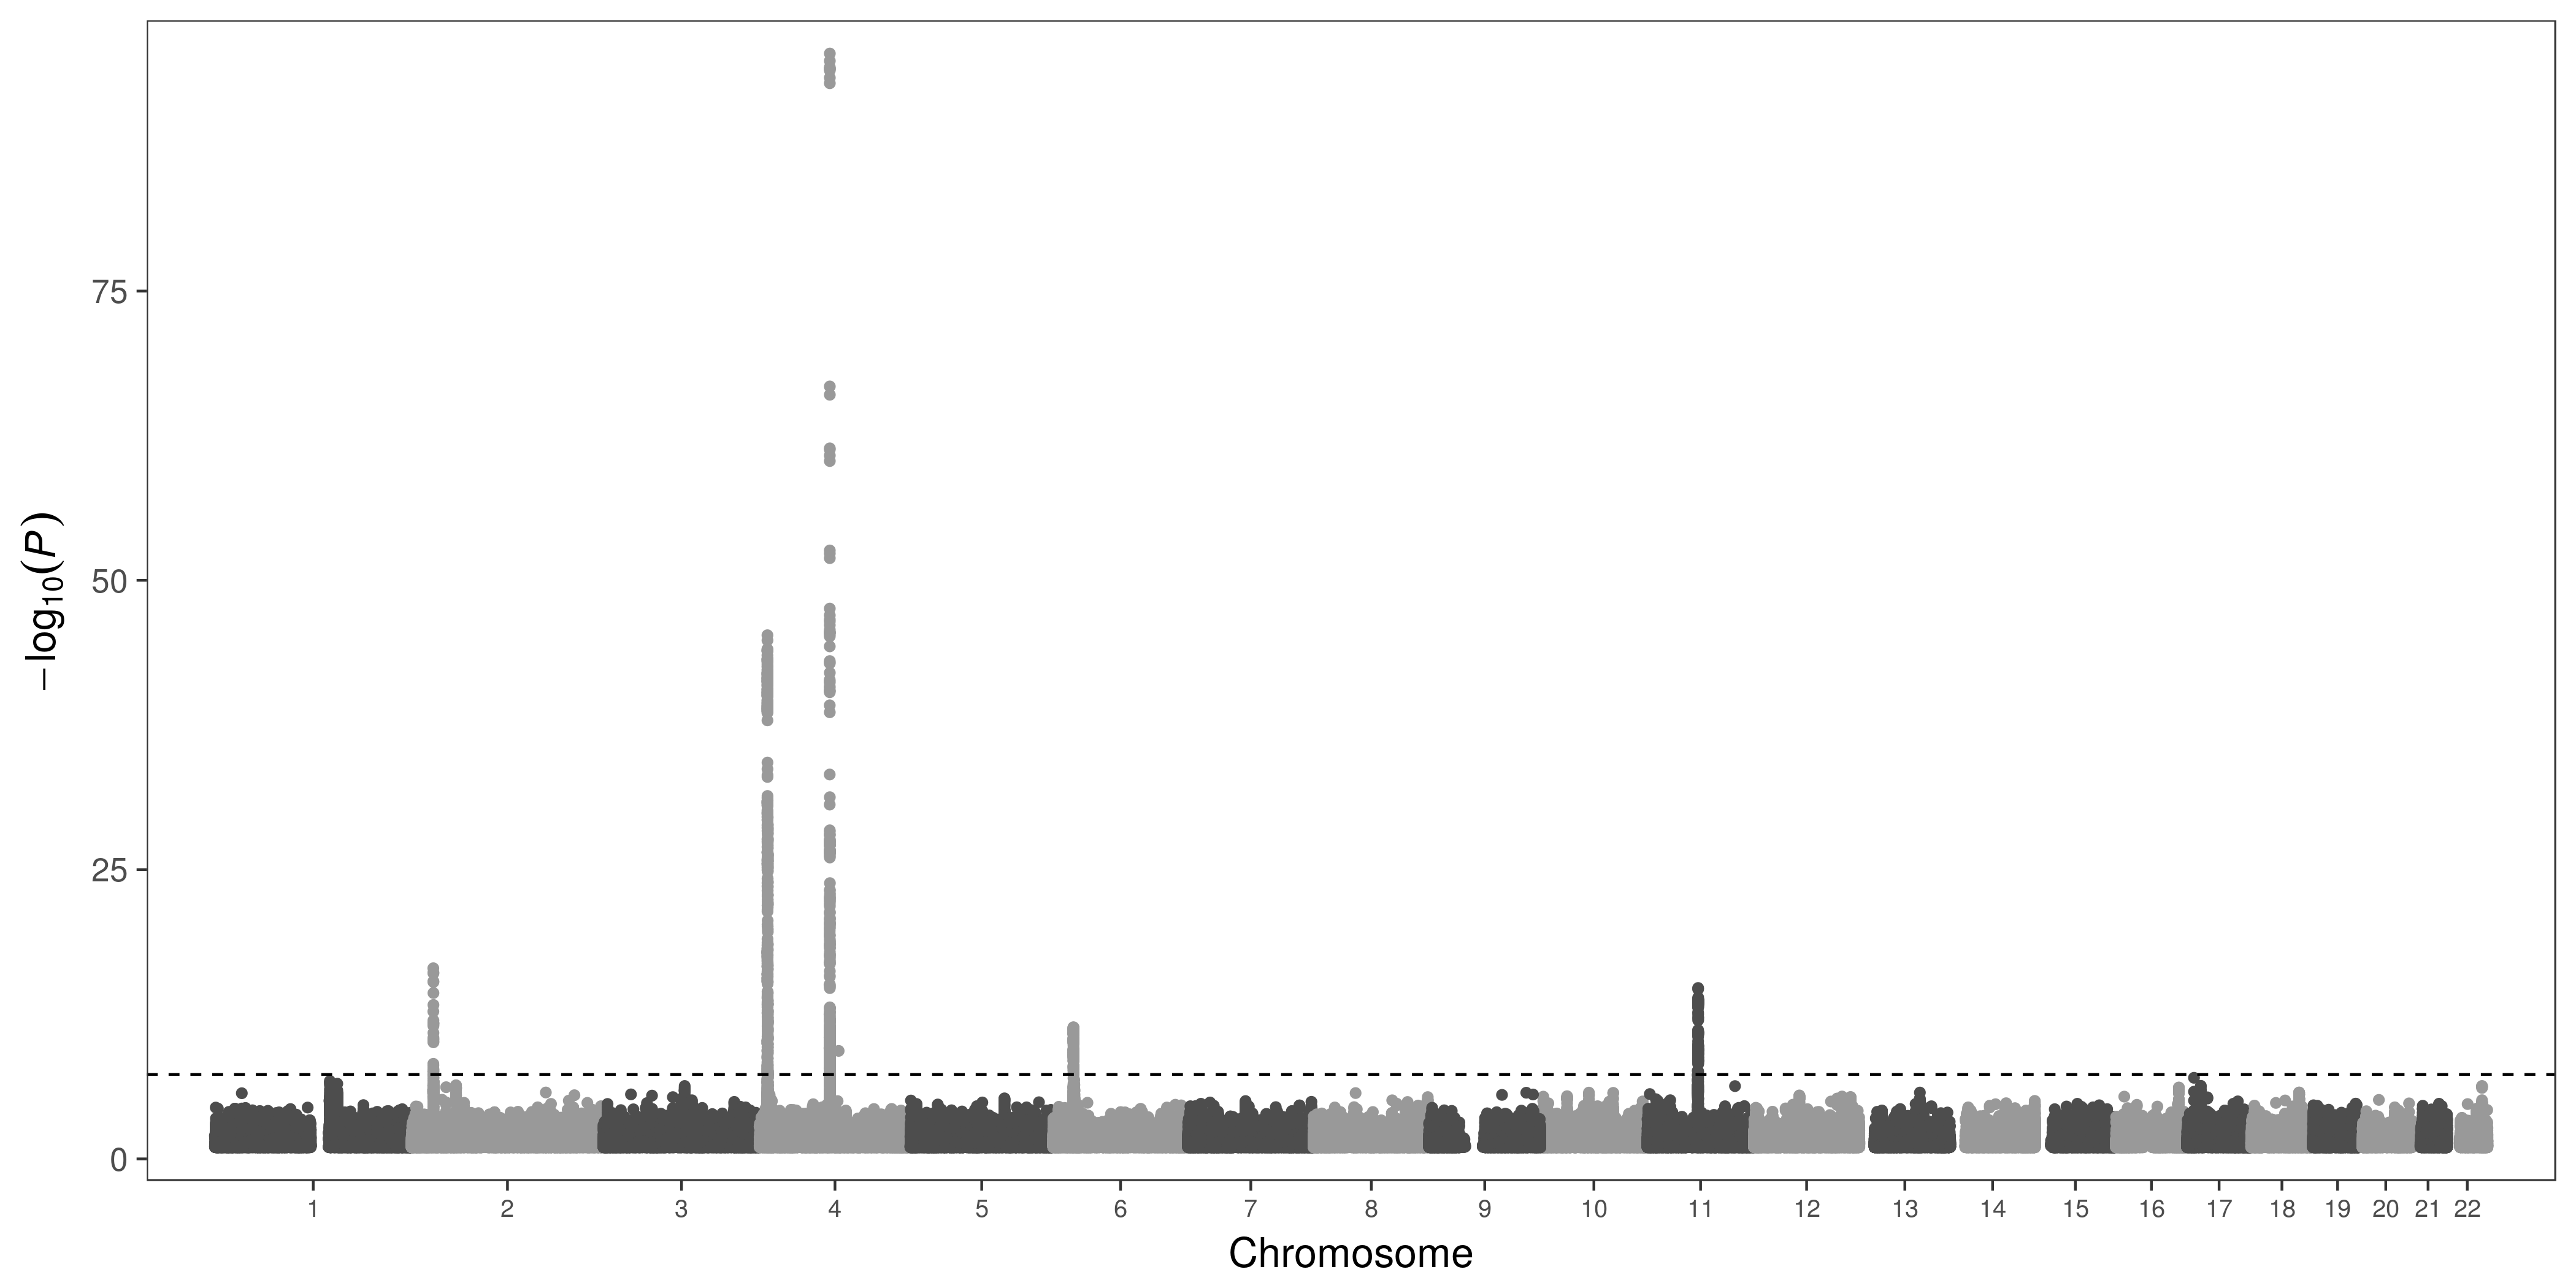
\includegraphics[width=0.95\linewidth]{images/05_selection_and_association/self_ult_age_sex_bmi} 

}

\caption[Manhattan plot for association with gout, adjusted for age, sex and \acrshort{bmi} using the self-reported gout or \acrshort{ult} usage gout definition.]{Manhattan plot for association with gout,
adjusted for age, sex and \gls{bmi} using the self-reported gout or
\gls{ult} usage gout definition. The dotted line indicates the
genome-wide significance threshold level of 5x10\textsuperscript{-8}.
The genome-wide significant peaks in order are \emph{GCKR} (chr2),
\emph{SLC2A9} and \emph{ABGC2} (chr4), \emph{SLC17A1-SLC17A3} (chr6),
and \emph{NRXN2-SLC22A12} (chr11).}\label{fig:manhatSelfUltAgeSexBmi}
\end{figure}




\FloatBarrier

\subsubsection{Polynesian GWAS}\label{polynesian-gwas}

The \gls{gwas} for gout in the Polynesian populations of New Zealand had
a total of 2402 individuals, with a mean age of 48.6 (\acrshort{sd}
14.9), was 60.5\% male, and had a mean \gls{bmi} of 35.0 (\acrshort{sd}
8.35). A break down by gout affection is shown in Table
\ref{tab:polyGwasclinc}. There were only two markers that met the
threshold for genome-wide significance, rs2725215 (risk allele = T,
\acrshort{or} = 1.939, 95\% CI = 1.567-2.40, P = 1.162 x
10\textsuperscript{-9}), located in \emph{PKD2}, and rs2231142 (risk
allele = T, \acrshort{or} = 2.306, 95\% CI =1.891-2.81, P = 1.570 x
10\textsuperscript{-16}), located in \emph{ABCG2}. The \gls{ld}
r\textsuperscript{2} between these two markers was 0.58 (\gls{pol}). Two
other markers reached the nominal significance threshold, rs2728108
(\emph{ABCG2}) and rs11034401 (chr11 inter-genic). Other genes that had
\glspl{snp} that were close to the nominal significance threshold, in
the 10\textsuperscript{-5} \textless{} P \textless{}
10\textsuperscript{-4} range contained some previously associated
genes/regions for urate and gout such as \emph{SLC2A9} and the region
containing \emph{IBSP}, \emph{MEPE}, \emph{PKD2}, and \emph{ABCG2}, all
on chromosome 4 (Figure \ref{fig:polyManhat}). Of the 39 \glspl{snp} in
the 10\textsuperscript{-4} \textgreater{} P \textgreater{}
10\textsuperscript{-5} range, only rs3775948 in \emph{SLC2A9},
rs7698623, rs2725220 and, rs1871744 in \emph{ABCG2}, rs6481407 in
\emph{BICC1}, and rs6041522 in \emph{LOC105372532}, had associations of
P \textless{} 0.05 in the UK Biobank gout \gls{gwas}, with only
rs3775948 being genome-wide significant (P = 9 x
10\textsuperscript{-43}).

\begin{table}

\caption{\label{tab:unnamed-chunk-16}\label{tab:polyGwasclinc} Clinical details for participants of the Polynesian gout GWAS.}
\centering
\begin{tabular}[t]{lcclcclcc}
\toprule
 & Controls & Cases\\
\midrule
n & 1182 & 1222\\
Mean Age (SD) & 44.14 (15.26) & 52.95 (13.2)\\
Mean BMI (SD) & 33.35 (8.12) & 36.62 (8.26)\\
Sex (\% Male) & 43.9 & 81.4\\
\bottomrule
\multicolumn{9}{l}{Mean age is reported in years. BMI is reported in kg/m\textsuperscript{2}.}\\
\end{tabular}
\end{table}








\begin{figure}

{\centering 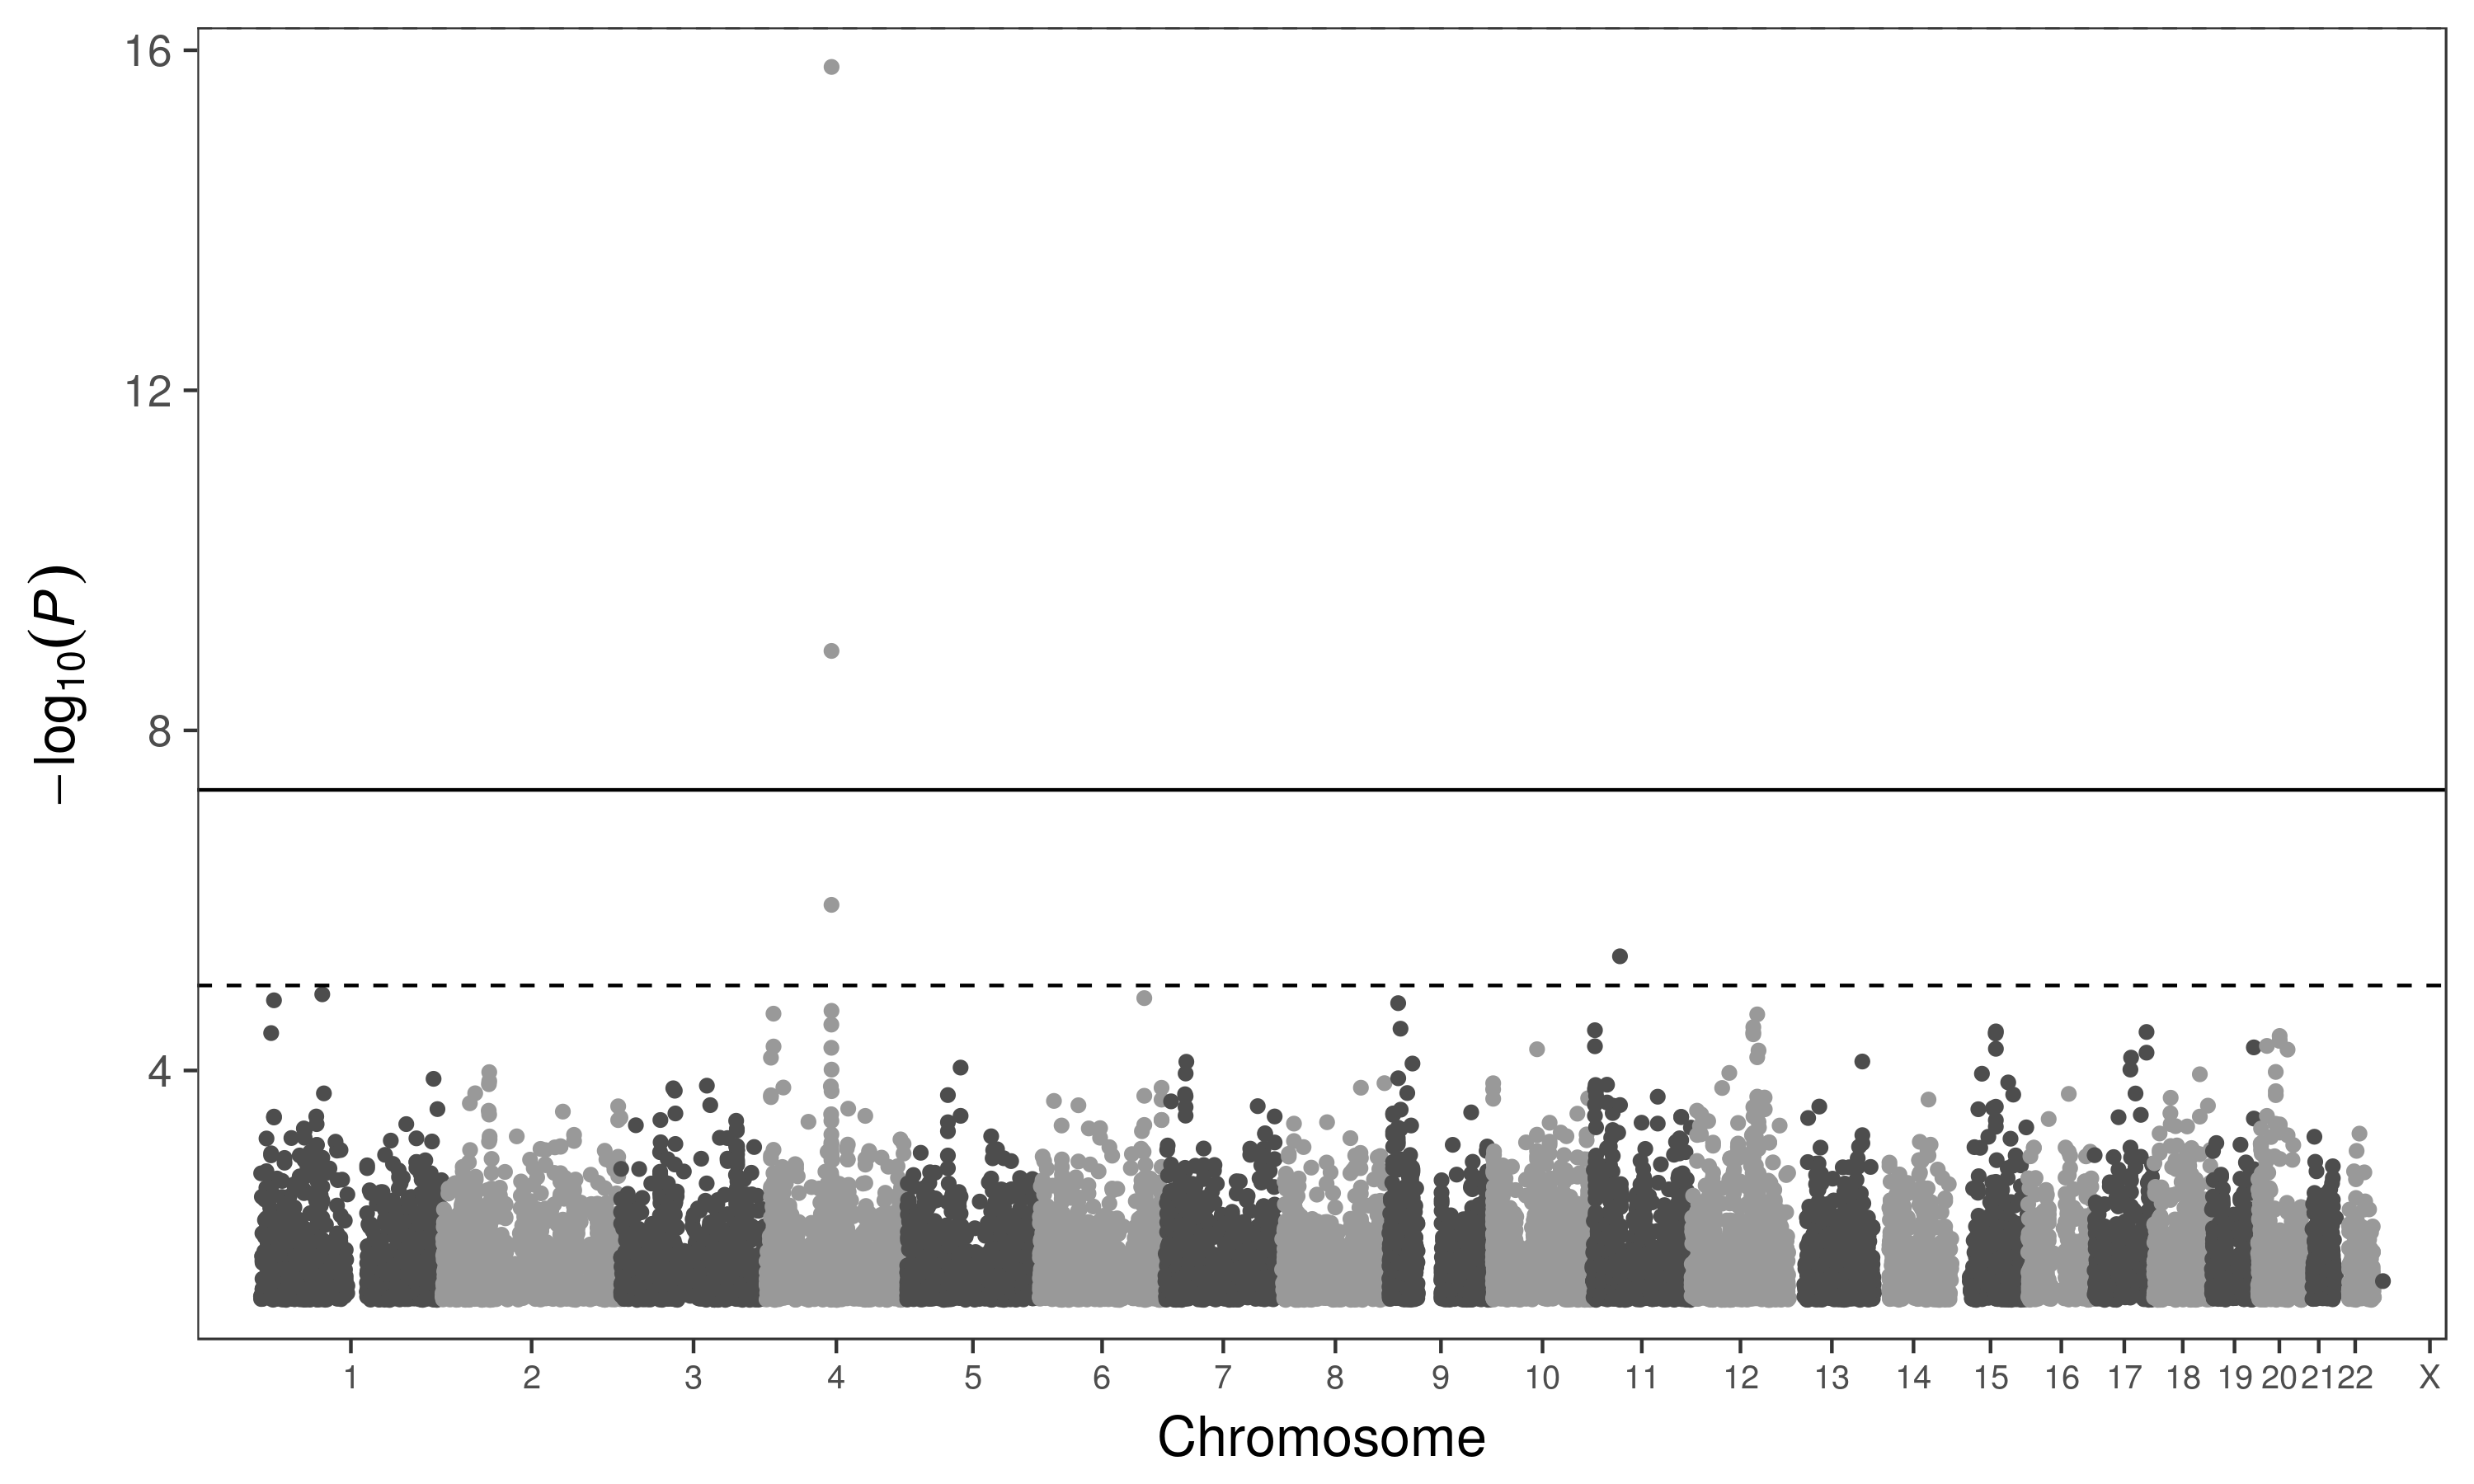
\includegraphics[width=0.95\linewidth]{images/05_selection_and_association/polyGwas} 

}

\caption[Manhattan plot for gout GWAS, adjusted for age and sex, in Polynesian ancestry individuals.]{Manhattan plot for gout GWAS, adjusted for age and sex,
in Polynesian ancestry individuals showing -log\textsubscript{10}(P) for
the association test by genomic position. The solid line indicates the
genome-wide significance threshold of P = 5 x10\textsuperscript{-8}, the
dashed line indicates the suggestive significance threshold of P =
10\textsuperscript{-5}.}\label{fig:polyManhat}
\end{figure}

\subsection{Comparison of haplotypic selection with gout
GWAS}\label{comparison-of-haplotypic-selection-with-gout-gwas}

In order to determine if additional loci (which did not meet the
significance threshold in \gls{gwas}), had extra information from the
selection tests that could prioritise the \gls{gwas} results, the gout
\gls{gwas} and selection results were combined. The ``European
Ancestry'' combination, combined the \gls{gwas} performed in the UK
Biobank using the self-reported gout or \gls{ult} usage with the
haplotypic selection results for the \gls{gbr} population. The
``Polynesian Ancestry'' combination, combined the Polynesian gout
\gls{gwas} with the haplotypic selection results for the Polynesian
populations of \gls{cim}, \gls{nzm}, \gls{sam}, and \gls{ton}. All of
the analyses were restricted to the markers of the CoreExome \gls{snp}
array. A new threshold for the combinations was used that required an
\textbar{}\gls{ihs}\textbar{} \textgreater{} 2 or
\textbar{}\gls{nsl}\textbar{} \textgreater{} 2 and a \gls{gwas} P
\textless{} 2 x 10\textsuperscript{-4}. the \gls{ihs} and \gls{nsl}
threshold was selected because \textbar{}\gls{ihs}\textbar{} or
\textbar{}\gls{nsl}\textbar{} \textgreater{} 2 is equivalent to P
\textless{} 0.05, since the statistics are very similar to a Z-score. A
``probability score'' for the combined statistics was calculated using
Score\textsubscript{combined} = P\textsubscript{GWAS} x
P\textsubscript{selection}, where P\textsubscript{selection} was given
by 1 - P(\textbar{}Z\textbar{}), and Z was the \gls{ihs} or \gls{nsl}
value. With the Polynesian populations, the maximum
\textbar{}value\textbar{} was used. The combined threshold was set as
Score\textsubscript{combined} \textless{} 5 x 10\textsuperscript{-8}, to
mirror the \gls{gwas} significance threshold.

\subsubsection{UK Biobank GWAS and haplotypic selection in
GBR}\label{uk-biobank-gwas-and-haplotypic-selection-in-gbr}

When the results from the UK Biobank \gls{gwas} for gout (using the
self-reported gout or \gls{ult} usage definition) and the \gls{ihs} and
\gls{nsl} results for the \gls{gbr} population were combined, there was
only one \gls{snp}, rs12638016 (intergenic), with an
\textbar{}\gls{ihs}\textbar{} \textgreater{} 2.6 (equivalent to the most
extreme 1\%) that also had P \textless{} 10\textsuperscript{-5} in the
\gls{gwas}. If the significance threshold for \gls{ihs} was reduced to
\textbar{}\gls{ihs}\textbar{} \textgreater{} 2 (approximately the 5\%
extreme most values), then there were three \glspl{snp}, all located at
\emph{SLC22A12} or within 1 kb, that were genome-wide significant in the
\gls{gwas} (rs505802, rs9734313, and rs559946), and four \glspl{snp}
that were nominally significant. There were 176 \glspl{snp} that had an
\textbar{}\gls{ihs}\textbar{} \textgreater{} 2 and a gout \gls{gwas} of
P \textless{} 0.01. This decreased to ten \glspl{snp}, when the
\gls{gwas} P threshold was reduced to 2 x 10\textsuperscript{-4} (Table
\ref{tab:haplogwas}). Only the variants in \emph{SLC22A12} replicated in
the UK Biobank replication cohort.

Using a threshold of \textbar{}\gls{nsl}\textbar{} \textgreater{} 2 and
a nominally significant P \textless{} 10\textsuperscript{-5}, two
\glspl{snp} were identified, both on chromosome 6 (Table
\ref{tab:haplogwas}). The first was rs4712972, located in
\emph{SLC17A4.} The second was rs501220, located in \emph{SLC17A3}. If
the thresholds were relaxed, there were 158 \glspl{snp} that had a
\textbar{}\gls{nsl}\textbar{} \textgreater{} 2 and a gout \gls{gwas} P
\textless{} 0.01. This decreased to seven, when a \gls{gwas} P threshold
of 2 x 10\textsuperscript{-4} was used (Table \ref{tab:haplogwas}). The
only variants that replicated in the UK Biobank replication cohort were
from \emph{SLC17A3} and \emph{SLC17A4}.

\begin{landscape}\begin{table}

\caption{\label{tab:ukhaplogwas}\label{tab:haplogwas} SNPs that had |iHS| or |nSL| > 2 from the GBR, 1000 Genomes Project population and a gout association P > 2 x 10\textsuperscript{-4} in the UK Biobank self-reported gout or ULT definition.}
\centering
\resizebox{\linewidth}{!}{
\begin{tabular}[t]{rrllllllllll}
\toprule
\multicolumn{1}{c}{} & \multicolumn{1}{c}{} & \multicolumn{1}{c}{} & \multicolumn{1}{c}{} & \multicolumn{1}{c}{} & \multicolumn{1}{c}{} & \multicolumn{1}{c}{} & \multicolumn{1}{c}{Selection} & \multicolumn{2}{c}{GWAS} & \multicolumn{1}{c}{} & \multicolumn{1}{c}{} \\
\cmidrule(l{2pt}r{2pt}){8-8} \cmidrule(l{2pt}r{2pt}){9-10}
Chromsome & Position & Marker & Gene name & Ref & Alt & Anc & GBR & A1 & OR [95\% CI], P & Score combined & UKBB Rep (OR [95\% CI], P)\\
\midrule
\addlinespace[0.3em]
\multicolumn{12}{l}{\textbf{iHS}}\\
\hspace{1em}2 & 27972833 & rs12104449 & \em{LOC105374378} & A & G & A & 2.213 & G & 1.275 [1.160-1.402], 4.638 x 10\textsuperscript{-7} & \textbf{6.230 x 10\textsuperscript{-9}} & 1.137 [1.071-1.208], 2.842 x 10\textsuperscript{-5}\\
\hspace{1em}3 & 166249372 & rs12638016 & \em{} & C & T & C & 2.632 & T & 0.883 [0.830-0.939], 8.101 x 10\textsuperscript{-5} & 3.438 x 10\textsuperscript{-7} & 1.002 [0.962-1.044], 0.914\\
\hspace{1em}10 & 3628517 & rs11251954 & \em{LOC105376360} & G & A & G & 2.075 & A & 1.140 [1.067-1.218], 9.698 x 10\textsuperscript{-5} & 1.842 x 10\textsuperscript{-6} & 1.002 [0.958-1.048], 0.939\\
\hspace{1em}11 & 64357072 & rs505802 & \em{SLC22A12} & T & C & C & 2.220 & C & 1.246 [1.169-1.328], 1.255 x 10\textsuperscript{-11} & \textbf{1.659 x 10\textsuperscript{-13}} & 1.228 [1.176-1.282], 8.670 x 10\textsuperscript{-21}\\
\hspace{1em}11 & 64358311 & rs9734313 & \em{SLC22A12} & C & T & C & 2.220 & C & 1.246 [1.169-1.328], 1.267 x 10\textsuperscript{-11} & \textbf{1.674 x 10\textsuperscript{-13}} & 1.226 [1.174-1.280], 1.811 x 10\textsuperscript{-20}\\
\hspace{1em}11 & 64358605 & rs559946 & \em{SLC22A12} & T & C & C & 2.220 & C & 1.247 [1.170-1.329], 1.065 x 10\textsuperscript{-11} & \textbf{1.407 x 10\textsuperscript{-13}} & 1.227 [1.175-1.281], 1.111 x 10\textsuperscript{-20}\\
\hspace{1em}12 & 112871372 & rs11066301 & \em{PTPN11} & A & G & A & 2.469 & G & 1.136 [1.070-1.206], 3.198 x 10\textsuperscript{-5} & 2.167 x 10\textsuperscript{-7} & 1.062 [1.020-1.106], 0.004\\
\hspace{1em}15 & 58970805 & rs7182060 & \em{ADAM10} & T & G & T & -2.060 & G & 0.824 [0.752-0.903], 3.182 x 10\textsuperscript{-5} & 6.262 x 10\textsuperscript{-7} & 1.017 [0.961-1.077], 0.555\\
\hspace{1em}16 & 79943738 & rs7185008 & \em{} & G & A & G & -2.220 & A & 1.215 [1.111-1.328], 1.800 x 10\textsuperscript{-5} & 2.378 x 10\textsuperscript{-7} & 1.047 [0.985-1.114], 0.142\\
\hspace{1em}21 & 37953187 & rs432137 & \em{} & A & G & G & -2.840 & A & 1.123 [1.056-1.194], 1.992 x 10\textsuperscript{-4} & 4.494 x 10\textsuperscript{-7} & 1.017 [0.976-1.059], 0.432\\
\addlinespace[0.3em]
\multicolumn{12}{l}{\textbf{nSL}}\\
\hspace{1em}3 & 166249372 & rs12638016 & \em{} & C & T & C & 2.450 & T & 0.883 [0.830-0.939], 8.101 x 10\textsuperscript{-5} & 5.784 x 10\textsuperscript{-7} & 1.002 [0.962-1.044], 0.914\\
\hspace{1em}6 & 25772047 & rs4712972 & \em{SLC17A4} & A & G & G & 2.306 & A & 1.202 [1.111-1.301], 5.202 x 10\textsuperscript{-6} & 5.489 x 10\textsuperscript{-8} & 1.103 [1.044-1.165], 4.401 x 10\textsuperscript{-4}\\
\hspace{1em}6 & 25873025 & rs501220 & \em{SLC17A3} & C & A & C & 2.478 & A & 1.225 [1.130-1.327], 7.820 x 10\textsuperscript{-7} & \textbf{5.169 x 10\textsuperscript{-9}} & 1.125 [1.065-1.189], 2.910 x 10\textsuperscript{-5}\\
\hspace{1em}11 & 1150353 & rs17859811 & \em{MUC5AC} & G & A & g & -2.100 & A & 1.165 [1.076-1.261], 1.648 x 10\textsuperscript{-4} & 2.947 x 10\textsuperscript{-6} & 1.024 [0.970-1.081], 0.395\\
\hspace{1em}15 & 58970805 & rs7182060 & \em{ADAM10} & T & G & T & -2.367 & G & 0.824 [0.752-0.903], 3.182 x 10\textsuperscript{-5} & 2.850 x 10\textsuperscript{-7} & 1.017 [0.961-1.077], 0.555\\
\hspace{1em}16 & 79943738 & rs7185008 & \em{} & G & A & G & -2.747 & A & 1.215 [1.111-1.328], 1.800 x 10\textsuperscript{-5} & 5.409 x 10\textsuperscript{-8} & 1.047 [0.985-1.114], 0.142\\
\hspace{1em}21 & 37953187 & rs432137 & \em{} & A & G & G & -2.984 & A & 1.123 [1.056-1.194], 1.992 x 10\textsuperscript{-4} & 2.838 x 10\textsuperscript{-7} & 1.017 [0.976-1.059], 0.432\\
\bottomrule
\multicolumn{12}{l}{GWAS results are age, sex and BMI adjusted. Ref is the reference allele in GRCh37, Alt is the alternative allele, Anc is the ancestral allele, and}\\
\multicolumn{12}{l}{A1 is the effect allele. Score combined < 5 x 10\textsuperscript{-8} is in bold.}\\
\end{tabular}}
\end{table}
\end{landscape}

\subsubsection{Polynesian GWAS and haplotypic selection in Polynesian
populations}\label{polynesian-gwas-and-haplotypic-selection-in-polynesian-populations}

Combining the results of the \gls{gwas} for gout in Polynesians with the
results of the \gls{ihs} analysis produced a single marker that met the
threshold of an \textbar{}\gls{ihs}\textbar{} \textgreater{} 2.6 and a
\gls{gwas} P \textless{} 5 x 10\textsuperscript{-8}; that \gls{snp} was
rs2725215, located in \emph{PKD2.} Rs2725215 also had a
\textbar{}\gls{nsl}\textbar{} \textgreater{} 2.6. Both \gls{ihs} and
\gls{nsl} thresholds were only met for \gls{ton}. There were 1604
\glspl{snp} that had a \gls{gwas} P \textless{} 0.05 and an
\textbar{}\gls{ihs}\textbar{} \textgreater{} 2; this reduced to 11 at
the combined threshold of \textbar{}\gls{ihs}\textbar{} \textgreater{} 2
and P \textless{} 2 x 10\textsuperscript{-4} (Table
\ref{tab:polyhaplogwas}). Combining the \gls{nsl} results with the
\gls{gwas}, there were 1502 \glspl{snp} that had a \gls{gwas} P
\textless{} 0.05 and a \textbar{}\gls{nsl}\textbar{} \textgreater{} 2;
this reduced to 14 at the combined threshold of
\textbar{}\gls{nsl}\textbar{} \textgreater{} 2 and P \textless{} 2 x
10\textsuperscript{-4} (Table \ref{tab:polyhaplogwas}).

At the combined threshold of \textbar{}\gls{ihs}\textbar{}
\textgreater{} 2 or \textbar{}\gls{nsl}\textbar{} \textgreater{} 2 and a
\gls{gwas} P \textless{} 2 x 10\textsuperscript{-4}, there were seven
\glspl{snp}, located within \emph{IBSP}, \emph{PKD2}, \emph{ABCG2} and
\emph{PPCDC}, found with both \gls{ihs} and \gls{nsl} (Table
\ref{tab:polyhaplogwas}). \emph{CHN2} and \emph{SLC39A11} only had
\glspl{snp} that met the \gls{nsl} threshold. Out of all of the
\glspl{snp} that met the combined threshold, ten \glspl{snp} had
evidence from both \gls{ihs} and \gls{nsl}. Rs12908919 (\emph{PPCDC})
was the only \gls{snp} that showed significance in multiple populations
(\gls{sam} and \gls{ton}) and had support from both \gls{ihs} and
\gls{nsl} (Table \ref{tab:polyhaplogwas}), whereas, there were six
\glspl{snp} that had support from only the \gls{ton} population, for
both \gls{ihs} and \gls{nsl}. The loci represented were different to the
\glspl{snp} in the European ancestry \gls{gwas} and selection analysis.

The region containing \emph{IBSP}, \emph{PKD2}, and \emph{ABCG2} had
multiple \glspl{snp} that met the suggestive significance threshold. Of
those, six \glspl{snp} had evidence of both selection and association
(Figure \ref{fig:locusZoom}, Table \ref{tab:polyhaplogwas}). The
selection signal came only from the Western Polynesian populations, with
no indication in the Eastern Polynesian populations of selection in this
region. The recombination rate in this region had intermittent small
spikes, with three of the variants in \emph{PDK2} having an \gls{ld}
R\textsuperscript{2} \textgreater{} 0.4 with rs2231142 (calculated using
\gls{eas}). These variants also had an association with gout that met
the suggestive significance threshold. Only the variants from
\emph{PKD2} and \emph{ABCG2} replicated their association from the UK
Biobank replication cohort.










\begin{figure}

{\centering 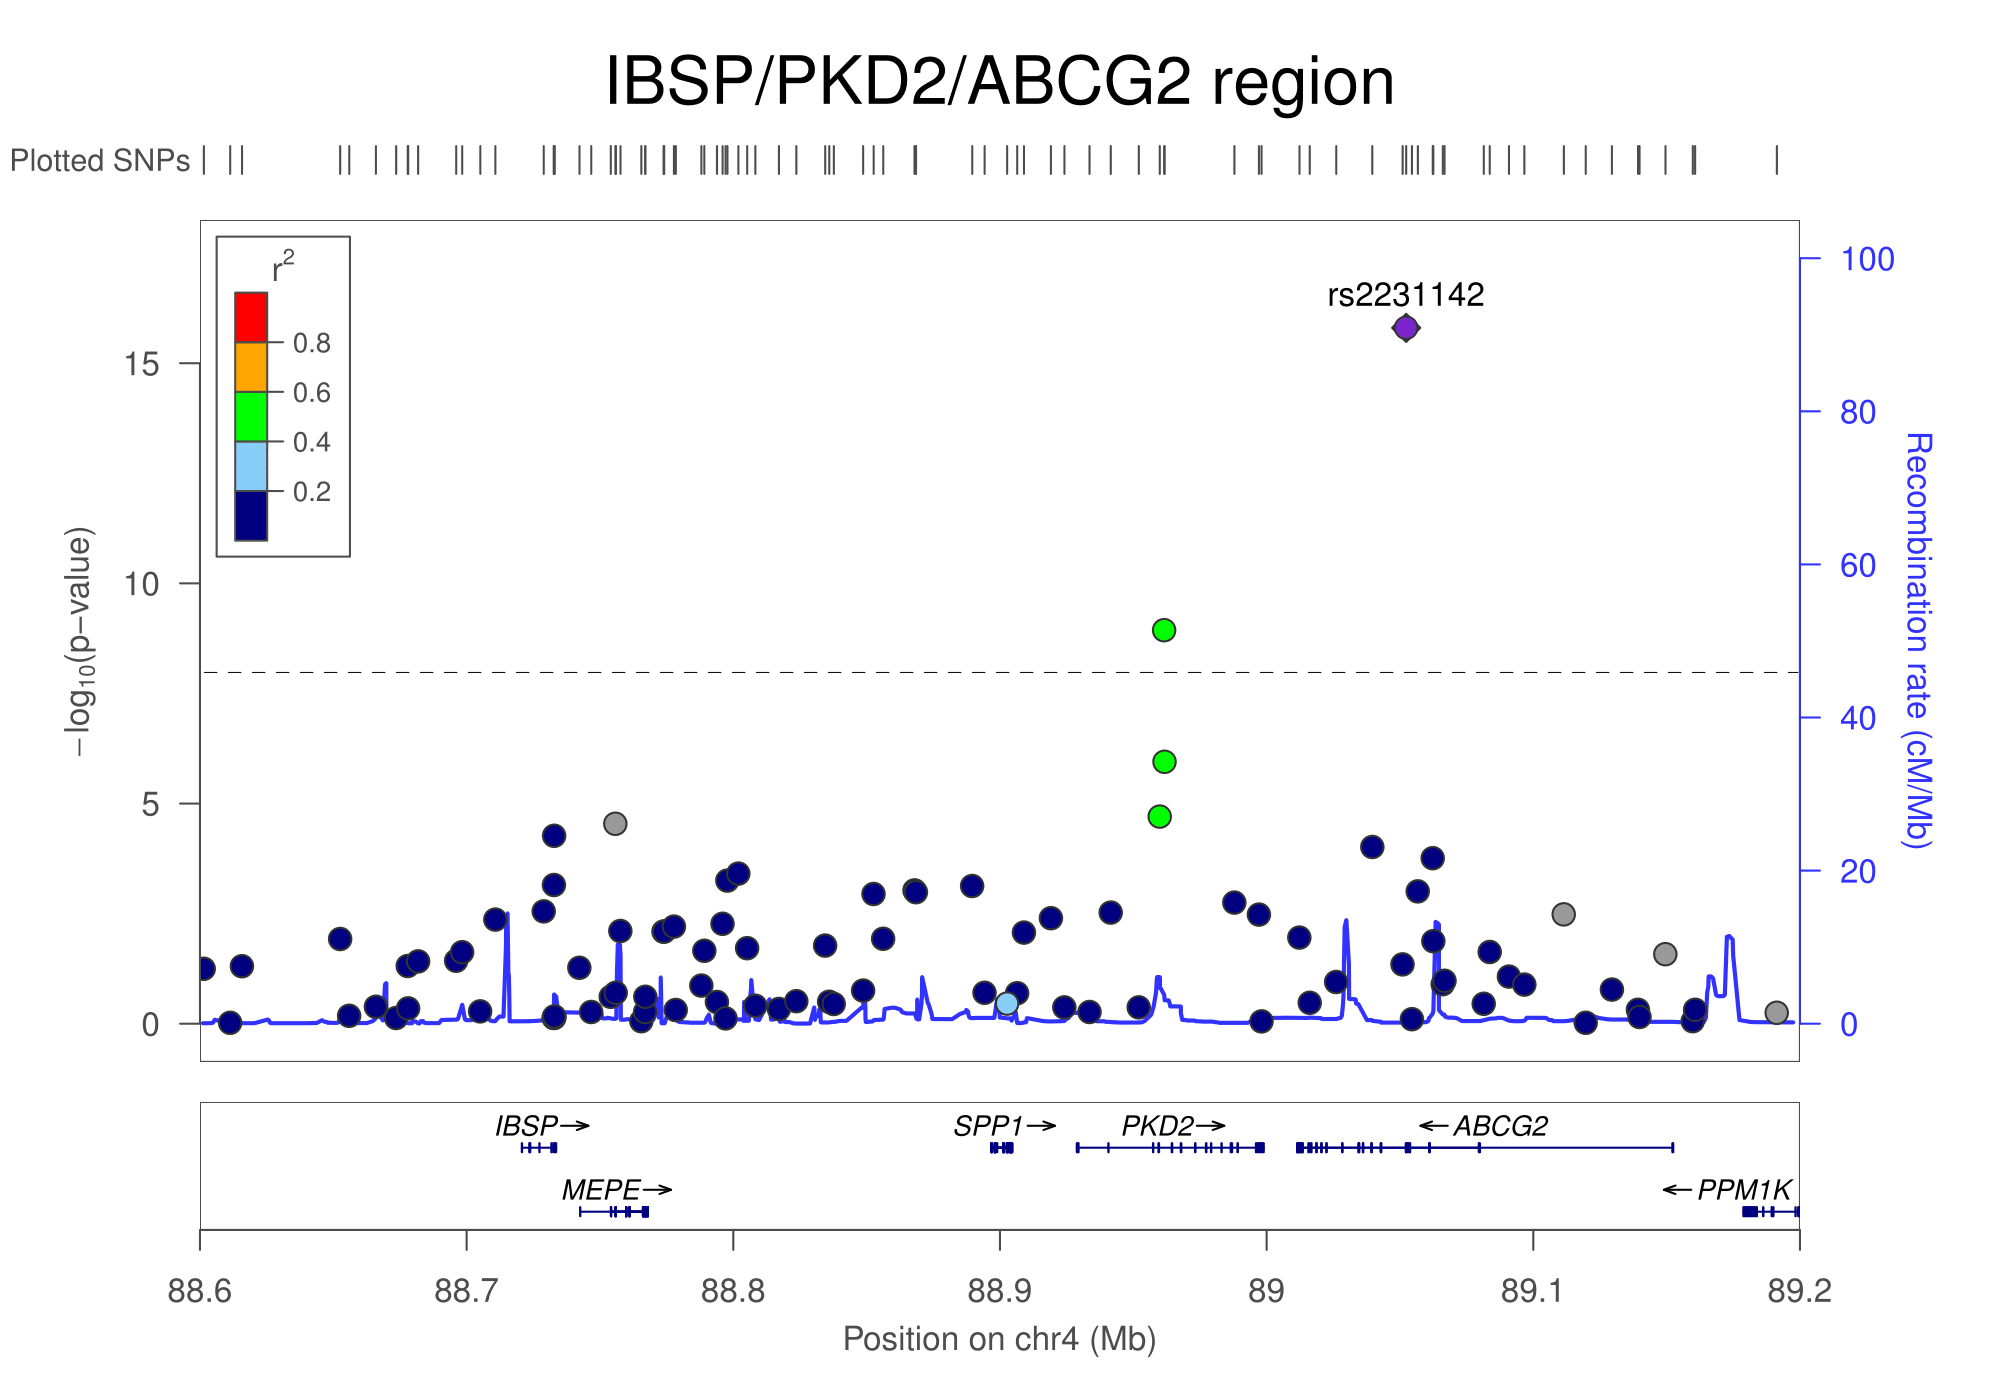
\includegraphics[width=0.8\linewidth]{images/05_selection_and_association/polygwas_locuszoom.ASN.chr4.88.6-89.2mb-1} 

}

\caption[Locus zoom plot of Polynesian gout \acrshort{gwas} results for the region covering \textit{IBSP}, \textit{PKD2}, and \textit{ABCG2}]{Locus zoom plot of Polynesian gout \gls{gwas} results
for the region chr4:88,600,000-89,200,000, covering \emph{IBSP},
\emph{PKD2}, and \emph{ABCG2}. Points indicate SNP association with gout
by genomic position in the Polynesian gout GWAS. Linkage disequilibrium
with rs2231142 is indicated by colour. Recombination rate in the East
Asian super population of the 1000 Genomes Project is indicated by the
blue line. The dashed line indicates the Genome-wide significance
threshold P = 5 x 10\textsuperscript{-8}.}\label{fig:locusZoom}
\end{figure}

\begin{landscape}\begin{table}

\caption{\label{tab:polyhaplogwastab}\label{tab:polyhaplogwas} SNPs that had |iHS| or |nSL| > 2 in the New Zealand Polynesian populations and a gout association P > 2 x 10\textsuperscript{-4} in the Polynesian GWAS.}
\centering
\resizebox{\linewidth}{!}{
\begin{tabular}[t]{rrlllllllllllll}
\toprule
\multicolumn{1}{c}{} & \multicolumn{1}{c}{} & \multicolumn{1}{c}{} & \multicolumn{1}{c}{} & \multicolumn{1}{c}{} & \multicolumn{1}{c}{} & \multicolumn{1}{c}{} & \multicolumn{4}{c}{Selection} & \multicolumn{2}{c}{GWAS} & \multicolumn{1}{c}{} & \multicolumn{1}{c}{} \\
\cmidrule(l{2pt}r{2pt}){8-11} \cmidrule(l{2pt}r{2pt}){12-13}
Chromosome & Position & Marker & Gene name & Ref & Alt & Anc & CIM & NZM & SAM & TON & A1 & OR [95\% CI], P & Score combined & UKBB Rep (OR [95\% CI], P)\\
\midrule
\addlinespace[0.3em]
\multicolumn{15}{l}{\textbf{iHS}}\\
\hspace{1em}4 & 88732874 & rs17013182 & \em{IBSP} & A & G & A & - & - & 1.544 & 2.550 & G & 1.596 [1.272-2.002], 5.410 x 10\textsuperscript{-5} & 2.910 x 10\textsuperscript{-7} & 1.079 [0.950-1.225], 0.244\\
\hspace{1em}4 & 88959922 & rs2725220 & \em{PKD2} & G & C & C & 0.266 & 0.863 & -1.800 & -2.866 & C & 1.466 [1.230-1.748], 1.988 x 10\textsuperscript{-5} & \textbf{4.138 x 10\textsuperscript{-8}} & 1.142 [1.097-1.189], 1.019 x 10\textsuperscript{-10}\\
\hspace{1em}4 & 88961571 & rs2725215 & \em{PKD2} & C & T & T & - & - & -1.952 & -2.866 & T & 1.939 [1.567-2.400], 1.162 x 10\textsuperscript{-9} & \textbf{2.419 x 10\textsuperscript{-12}} & 1.770 [1.671-1.875], 4.022 x 10\textsuperscript{-84}\\
\hspace{1em}4 & 88961736 & rs2728108 & \em{PKD2} & A & C & C & 0.270 & 0.728 & -1.579 & -2.738 & C & 1.546 [1.297-1.843], 1.127 x 10\textsuperscript{-6} & \textbf{3.479 x 10\textsuperscript{-9}} & 1.150 [1.105-1.198], 1.341 x 10\textsuperscript{-11}\\
\hspace{1em}4 & 89039629 & rs1871744 & \em{ABCG2} & T & C & T & -0.663 & -1.044 & -1.723 & -2.517 & C & 0.733 [0.627-0.857], 9.769 x 10\textsuperscript{-5} & 5.789 x 10\textsuperscript{-7} & 0.840 [0.795-0.888], 9.021 x 10\textsuperscript{-10}\\
\hspace{1em}4 & 89052323 & rs2231142 & \em{ABCG2} & G & T & G & -0.252 & - & 1.424 & 2.136 & T & 2.306 [1.891-2.813], 1.570 x 10\textsuperscript{-16} & \textbf{2.568 x 10\textsuperscript{-18}} & 2.098 [1.993-2.208], 6.608 x 10\textsuperscript{-177}\\
\hspace{1em}6 & 166567345 & rs6914547 & \em{} & G & A & A & 0.989 & 1.543 & 1.944 & 2.169 & A & 0.769 [0.671-0.881], 1.598 x 10\textsuperscript{-4} & 2.404 x 10\textsuperscript{-6} & 1.005 [0.965-1.047], 0.814\\
\hspace{1em}8 & 107908032 & rs6469084 & \em{} & A & G & G & -2.658 & -1.805 & -0.747 & -0.459 & G & 0.755 [0.652-0.874], 1.595 x 10\textsuperscript{-4} & 6.261 x 10\textsuperscript{-7} & 1.013 [0.959-1.071], 0.639\\
\hspace{1em}9 & 15521362 & rs7856710 & \em{} & G & A & A & -2.170 & -1.813 & 0.151 & 1.047 & A & 0.593 [0.463-0.758], 3.225 x 10\textsuperscript{-5} & 4.844 x 10\textsuperscript{-7} & 0.982 [0.899-1.073], 0.693\\
\hspace{1em}15 & 75348712 & rs12908919 & \em{PPCDC} & G & A & G & 1.443 & 1.308 & 2.692 & 2.493 & A & 1.457 [1.201-1.769], 1.383 x 10\textsuperscript{-4} & 4.907 x 10\textsuperscript{-7} & 1.057 [0.993-1.126], 0.083\\
\hspace{1em}17 & 55901677 & rs2685501 & \em{LOC105371839} & T & C & T & -0.136 & 1.367 & 0.907 & 2.170 & T & 1.377 [1.164-1.628], 1.866 x 10\textsuperscript{-4} & 2.800 x 10\textsuperscript{-6} & 1.039 [0.997-1.082], 0.068\\
\addlinespace[0.3em]
\multicolumn{15}{l}{\textbf{nSL}}\\
\hspace{1em}4 & 88732874 & rs17013182 & \em{IBSP} & A & G & A & - & - & 1.387 & 2.375 & G & 1.596 [1.272-2.002], 5.410 x 10\textsuperscript{-5} & 4.750 x 10\textsuperscript{-7} & 1.079 [0.950-1.225], 0.244\\
\hspace{1em}4 & 88959922 & rs2725220 & \em{PKD2} & G & C & C & 0.309 & 0.705 & -2.049 & -3.129 & C & 1.466 [1.230-1.748], 1.988 x 10\textsuperscript{-5} & \textbf{1.744 x 10\textsuperscript{-8}} & 1.142 [1.097-1.189], 1.019 x 10\textsuperscript{-10}\\
\hspace{1em}4 & 88961571 & rs2725215 & \em{PKD2} & C & T & T & - & - & -2.198 & -3.128 & T & 1.939 [1.567-2.400], 1.162 x 10\textsuperscript{-9} & \textbf{1.024 x 10\textsuperscript{-12}} & 1.770 [1.671-1.875], 4.022 x 10\textsuperscript{-84}\\
\hspace{1em}4 & 88961736 & rs2728108 & \em{PKD2} & A & C & C & 0.308 & 0.556 & -1.754 & -2.929 & C & 1.546 [1.297-1.843], 1.127 x 10\textsuperscript{-6} & \textbf{1.919 x 10\textsuperscript{-9}} & 1.150 [1.105-1.198], 1.341 x 10\textsuperscript{-11}\\
\hspace{1em}4 & 89039629 & rs1871744 & \em{ABCG2} & T & C & T & -0.691 & -1.168 & -1.724 & -2.488 & C & 0.733 [0.627-0.857], 9.769 x 10\textsuperscript{-5} & 6.277 x 10\textsuperscript{-7} & 0.840 [0.795-0.888], 9.021 x 10\textsuperscript{-10}\\
\hspace{1em}4 & 89052323 & rs2231142 & \em{ABCG2} & G & T & G & -0.489 & - & 1.440 & 2.146 & T & 2.306 [1.891-2.813], 1.570 x 10\textsuperscript{-16} & \textbf{2.500 x 10\textsuperscript{-18}} & 2.098 [1.993-2.208], 6.608 x 10\textsuperscript{-177}\\
\hspace{1em}5 & 56390346 & rs831831 & \em{} & A & G & G & 1.361 & 2.063 & 1.334 & 1.234 & A & 1.331 [1.145-1.547], 1.947 x 10\textsuperscript{-4} & 3.812 x 10\textsuperscript{-6} & 0.995 [0.946-1.046], 0.841\\
\hspace{1em}6 & 166567345 & rs6914547 & \em{} & G & A & A & 1.156 & 1.356 & 1.403 & 2.135 & A & 0.769 [0.671-0.881], 1.598 x 10\textsuperscript{-4} & 2.618 x 10\textsuperscript{-6} & 1.005 [0.965-1.047], 0.814\\
\hspace{1em}7 & 29213691 & rs6944596 & \em{CHN2} & C & T & C & -1.487 & -1.601 & -0.764 & -2.185 & T & 1.324 [1.152-1.522], 7.899 x 10\textsuperscript{-5} & 1.141 x 10\textsuperscript{-6} & 1.016 [0.938-1.101], 0.698\\
\hspace{1em}8 & 107908032 & rs6469084 & \em{} & A & G & G & -2.210 & -1.767 & -0.851 & -0.531 & G & 0.755 [0.652-0.874], 1.595 x 10\textsuperscript{-4} & 2.161 x 10\textsuperscript{-6} & 1.013 [0.959-1.071], 0.639\\
\hspace{1em}15 & 75348712 & rs12908919 & \em{PPCDC} & G & A & G & 1.429 & 1.419 & 2.340 & 2.198 & A & 1.457 [1.201-1.769], 1.383 x 10\textsuperscript{-4} & 1.334 x 10\textsuperscript{-6} & 1.057 [0.993-1.126], 0.083\\
\hspace{1em}17 & 55901677 & rs2685501 & \em{LOC105371839} & T & C & T & 0.352 & 1.221 & 1.166 & 2.355 & T & 1.377 [1.164-1.628], 1.866 x 10\textsuperscript{-4} & 1.730 x 10\textsuperscript{-6} & 1.039 [0.997-1.082], 0.068\\
\hspace{1em}17 & 70897198 & rs4969131 & \em{SLC39A11} & C & T & T & -1.257 & -0.913 & -2.121 & -1.963 & C & 0.732 [0.631-0.849], 3.527 x 10\textsuperscript{-5} & 5.981 x 10\textsuperscript{-7} & 1.018 [0.977-1.060], 0.394\\
\bottomrule
\multicolumn{15}{l}{GWAS results are age, sex, and PCA adjusted. Ref is the reference allele in GRCh37, Alt is the alternative allele, Anc is the ancestral allele, and}\\
\multicolumn{15}{l}{A1 is the effect allele. Score combined < 5 x 10\textsuperscript{-8} is in bold.}\\
\end{tabular}}
\end{table}
\end{landscape}

\section{Chapter Discussion}\label{chapter-discussion-1}

\subsection{Performance of gout
definition}\label{performance-of-gout-definition}

The UK Biobank had a larger number of cases for the gout \gls{gwas} than
\citet{Kottgen2013}. This increase in cases reflects the increase in
strength of association that was seen. A similar comparison of gout
definitions was performed using data from the study for updated gout and
classification criteria (SUGAR) with 983 rheumatology patients with
known gout affection and definitions derived from epidemiology studies
used in the Global Urate Genetics Consortium \gls{gwas} of
hyperuricaemia and gout were tested for sensitivity and specificity
\citep{Dalbeth2016}. In the SUGAR paper, the definition that provided
the highest specificity (82\%) and sensitivity (72\%) was self-reported
gout or on \gls{ult} when tested against the mono-sodium urate crystal
identification as the gold standard. Consistent with this, the work
presented here found that the self-report of gout or \gls{ult} use
definition also provided the highest precision from the definitions
used, and supports the use of this definition in genetic studies when
better gout classification methods are not available, such as \gls{acr}
criteria or mono-sodium urate crystal identification.

The different definitions of gout used in this study may represent the
different disease presentations or patient populations. Not all patients
were captured by all criteria, and the Winnard definition was not as
good as self-report of gout or \gls{ult}, despite a similarity in
definitions, and had lower precision in the genetic association. The
hospital diagnosis definition had the lowest prevalence and was
restrictive, making it the least likely to capture most people with
gout. One third of the people that met this definition did not meet any
of the self-report definitions, for gout, and/or \gls{ult} usage. There
is a number of reasons that might explain this. Firstly, the
hospitalised population may have a different disease presentation from
those in the community identified by self-report or \gls{ult} use.
Secondly, a diagnosis of gout made in a hospital may subsequently be
revised to a different diagnosis; this is not taken into account with
the current methodology. Therefore, when self-report information is
available it is recommended that the self-report of gout or \gls{ult}
use be used as the way to define cases.

Each of the gout definitions tested had genome-wide significance for
\glspl{snp} associated with gout in \emph{ABCG2} and \emph{SLC2A9}.
These two genes encode proteins that transport urate in the gut (ABCG2)
and proximal tubule of the kidney (SLC2A9). The large effect sizes in
the association with gout, show similarity with their large effect sizes
in the control of serum urate levels \citep{Kottgen2013}.

Heritability estimates for the variance attributed to the additive
effects of common \glspl{snp} for gout of 0.282-0.308 (excluding the
hospital definition) were in line with those reported by
\citet{Kottgen2013}, with the same approach using the GCTA software of
0.27 to 0.41 for serum urate levels. There was also no statistically
significant differences between the heritability estimates for the
different definitions. The comparability between the heritability
estimates for gout and serum urate by common genetic variants suggest
the genetic heritabilities of serum urate levels and gout is similar.
However, also contributing to the risk of gout are environmental
factors, such as diet and medications. Because the estimates are
constructed under an additive model, it does not account for the
non-additive variance, such as gene-gene or gene-environment
interactions, or rare variants, or the effect of structural variants
such as copy number variation.

\subsection{GWAS and selection}\label{gwas-and-selection}

The main peak of association in the Manhattan plots (Figures
\ref{fig:manhatSelfUltAgeSexBmi} and \ref{fig:polyManhat}) for the
\gls{gwas} analyses of both the UK Biobank, and the New Zealand
Polynesians was \emph{ABCG2}, this was consistent with previous
\gls{gwas} analyses for gout, compared to \gls{gwas} for serum urate
which has the strongest association with \emph{SLC2A9}
\citep{Okada2012, Kottgen2013, nakayama2017gwas}. Combining the
haplotypic selection results for \gls{ihs} and \gls{nsl} from the
\gls{gbr} population with the UK Biobank gout \gls{gwas} showed
additional evidence at \emph{SLC22A12}, \emph{PTPN11}, \emph{SLC17A3},
\emph{SLC17A4} , and \emph{ADAM10}. However, from the \gls{gwas} those
genes had already met the suggestive significance threshold of P
\textless{} 10\textsuperscript{-5}. All except \emph{ADAM10} had
previously been reported as being significant at a genome-wide threshold
for association with serum urate levels \citep{Kottgen2013}.
\emph{ADAM10} had not been previously associated at a genome-wide
threshold with either gout or serum urate levels, but had previously
been reported as a strong candidate for positive selection
\citep{Deschamps2016}. \emph{ADAM10} is involved in the innate immune
system with the Notch signalling pathway, but also becomes
down-regulated during interaction with the extracellular proteins
PfSEL1/PfSEL2 of \emph{P. falciparum} \citep{Singh2009}. The strength of
association weakened in the replication UK Biobank cohort for all loci
that had been identified, with most showing no signs of significance
except \emph{SLC22A12}, which increased in strength of association.

The combination of the New Zealand Polynesian gout \gls{gwas} with the
haplotypic selection statistics of \gls{ihs} and \gls{nsl} from the
Polynesian populations of \gls{cim}, \gls{nzm}, \gls{sam}, and \gls{ton}
did not have any corroboration with the equivalent combination of
analyses in the European ancestry cohort. The \gls{ton} population was
the main source of the selection statistics that met the threshold, this
could be due to the high proportion of gout patients (\textgreater{}
50\%) that were included in the sample. Between the \gls{ihs} and
\gls{nsl} based results, there was a high degree of overlap in the
\glspl{snp} that met the thresholds for both, although \gls{nsl} had
three \glspl{snp} that did not meet the threshold in \gls{ihs}.

The \emph{IBSP/PKD2/ABCG2} region has been associated with both gout and
urate levels \citep{Yang2010}, but often just the lead \gls{snp} of
rs2231142 is reported, as it has the strongest association and is one of
the most likely causative variants due to the Q141K amino acid change
that leads to a reduction in expression and a less efficient transporter
\citep{Woodward2009}. The \emph{IBSP} locus encodes bone sialoprotein,
which is involved with bone development \citep{Kerr1993}. Loci nearby
such as \emph{MEPE} and \emph{SPP1}, encode proteins with similar
structure and functions, suggesting a shared evolutionary history
\citep{Rowe2000}. In the presence of urate crystals, as with gout,
\emph{IBSP} expression is reduced and affects osteoblast differentiation
\citep{Chhana2011}. \emph{PKD2} is involved with kidney disease
\citep{Mochizuki1996, Hildebrandt2010}, and Polynesian populations have
a 3.5 fold higher incidence of end-stage renal disease, compared to
Europeans \citep{Collins2017book}. For all the variants that had both
selection and \gls{gwas} signal at \emph{PKD2}, the selection signal was
for the ancestral allele, which was also the risk allele for gout. The
selection signal was absent in the Eastern Polynesian populations, which
displayed selection statistics in favour of the derived/protective gout
alleles at \emph{PKD2}. As previously discussed (section
\ref{selectionDissussion}), many of the loci that have evidence
suggesting selection in Western Polynesian populations are calcium
channels. The \emph{IBSP/PKD2/ABCG2} region, is functionally involved
with calcium, bone sialoprotein has a high affinity for calcium
\citep{Kerr1993}, and PKD2 has some homology with calcium channels,
containing domains that are consistent with calcium binding
\citep{Mochizuki1996}, again demonstrating this calcium-related
selection pattern.

\subsection{Limitations}\label{limitations}

In the analysis of the different gout definitions, there was a
difference between the the definitions in the number of \glspl{snp} that
had a significant association with gout, with the hospital diagnosis
definition having the fewest. One of the key differences between the
definitions was the number of cases defined for each, ranging from 382
to 2295, which will have impacted on the power for each \gls{gwas} to
detect associations. Similar to the \gls{gwas} results from the
different gout definitions, the differences between heritability
estimates of the different definitions may too be impacted by the
differing numbers of cases. Due to computational reasons, only a
sub-sample of the controls was used in the calculation of the
heritability estimates. The use of all of the controls may have changed
the results of the heritability analysis. Another limitation of the
definitions was the lack of `gold standard' to which the definitions
could be compared, and therefore sensitivity and specificity were unable
to be calculated for each definition. The ancestry of the UK Biobank
samples included for the gout definitions were European, this means that
results and conclusions from the definition and heritability analysis
may not be applicable to other ancestral backgrounds.

With the combination of the selection statistics with the results of the
gout \gls{gwas} analyses, the variants that were able to be compared
were limited by the selection analysis, where the selection results were
only from the markers that were available on the CoreExome \gls{snp}
array. This is despite the UK Biobank \gls{gwas} being conducted on an
imputed dataset, where there were results for 9.3 million markers after
filtering. This compared to the total number of 236,868 markers for
which there were \gls{ihs} or \gls{nsl} results. It is possible that if
there were \gls{ihs} and \gls{nsl} results for a greater number of
markers, more loci may have been prioritised. The Polynesian \gls{gwas}
was limited by sample size, and also in the number of markers for which
there were both association and selection results. The marker density of
the CoreExome \gls{snp} array could have been improved through
imputation, however, for Polynesian populations, the public haplotype
reference panels lack representation of Polynesian populations. This
means that Polynesian specific variants (such as rs373863828,
\citet{Minster2016}) and therefore haplotypes, are not incorporated in
the imputation, and as a result the imputation accuracy suffers
\citep{Howie2011}.

The combination of the Eastern and Western Polynesian populations into a
single grouped population for the \gls{gwas} may also affect the
results, as there are population specific effects, even between similar
ancestral backgrounds such as the East and West Polynesian populations.
Such differences with respect to gout have been seen with \emph{ABCG2}
\citep{Phipps-Green2010}. This was similar to what was observed in the
selection results at the extended locus including \emph{IBSP, PKD2, and
ABCG2} displaying a difference between Eastern and Western Polynesian
populations. One method to take into account these differences between
the Eastern and Western Polynesian populations, would be to perform the
\gls{gwas} separately in each and then meta-analyse the results.

\subsection{Conclusions}\label{conclusions-1}

The analyses in this chapter for performance of the case-definition for
gout association studies showed that in the absence of the gold-standard
of observing urate crystals in the synovial fluid, or the \gls{acr}
criteria, it is recommended using the self-report or \gls{ult}
definition, as this gave the best performance in estimating the cohort
gout prevalence, out of the definitions tested in this analysis. It was
also shown that incorporation of selection analyses with \gls{gwas} does
provide evidence for additional variants associated with gout. Despite
these associations already mostly being nominally significant from
\gls{gwas}, the selection analyses do provide an avenue for
prioritisation of \gls{gwas} results but only appeared to further
enhance evidence at known loci, rather than aid in discovery. Further
work such as incorporating multiple selection statistics, and the use of
whole genome sequenced data or imputed genetic data would be useful to
improve the prioritising of \gls{gwas} results.

\chapter{Summary and Conclusions}\label{summary-and-conclusions}

\section{Summary}\label{summary}

This thesis set out to investigate the role of genetic selection in the
genome of modern Polynesian populations, and its effect on urate and
metabolic disease. There were three main objectives that were covered.
The first was to identify and characterise positive selection within
Polynesian populations with regard to metabolic diseases such as gout,
obesity, \gls{t2d}, kidney disease, and metabolic syndrome. The second
was to investigate the shared ancestral history of Polynesian
populations in genomic regions relevant to metabolic disease. The third
was to investigate the impact of alternative of gout definitions in
association studies, and to incorporate the use of selection statistics
into association analyses.

\subsection{Evidence of selection in Polynesian
populations}\label{evidence-of-selection-in-polynesian-populations}

Chapter \ref{selectionResults} utilised multiple selection and
neutrality statistics, based on haplotypic and frequency spectrum
methodologies, to establish regions of the genome that exhibited
`signals of selection'. The findings of Chapter \ref{selectionResults},
specifically identified regions of the genome in Polynesian populations
that had evidence suggesting that positive selection had played a role.
The characterisation of these regions through pathway analysis indicated
that metabolic functions dominated in the pathways with enrichment of
genes that had evidence of possible selection. However, only fractions
of the pathways were enriched. The majority of the genes in these
pathways were enriched for significant markers from \gls{nsl}. The
Eastern Polynesian populations had a greater number of enriched pathways
than the Western Polynesian populations. Many of the genes in the
pathways enriched in the Eastern Polynesian populations were involved
with signalling, specifically with calcium.

The enriched pathway in common between the Western Polynesian
populations was ABC transporters. The loci, \emph{ABCG2} and
\emph{ABCC4}, that encode for two ABC transporters, have previously had
genetic variants identified that increase risk of gout in Western
Polynesian populations \citep{Phipps-Green2010, Tanner2017}.
\emph{ABCC4} has also had a Western Polynesian specific \gls{snp}
(rs972711951) identified that associated with gout \citep{Tanner2017},
and there was evidence of possible selection at this locus, from
\gls{cim}, \gls{nzm}, and \gls{sam}.

The loci that exhibited `signatures of selection' in Polynesian
populations, that were also associated with urate were limited, and
there was minimal evidence for the main effect loci for urate and gout
of \emph{SLC2A9} and \emph{ABCG2}. Instead the loci that indicated
possible selection included \emph{RREB1}, \emph{IGFR1} and \emph{BCAS3},
none of which are urate transporters but instead are involved with more
central metabolic pathways. The other metabolic diseases of obesity,
\gls{t2d}, kidney disease, and metabolic syndrome all had a number of
associated loci that also had evidence of possible selection. Some of
these loci were associated with multiple traits, and had an
immunological function. This points to a potential relationship of these
loci being influenced by pathogenic challenge, that results in influence
on metabolic diseases. One example of this potential relationship could
be loci that were associated with obesity and \gls{t2d}, that were also
associated with malarial infection. One of the genes, \emph{DDC}, that
was putatively associated with malaria, had one of the strongest
\gls{ihs} signals in \gls{nzm}.

Due to urate having a central role in malaria infection and functioning
as an adjuvant for the innate immune system \citep{Ames1981, Opitz2009},
as well as previously having been identified a selective pressure
applied to the genome, malaria associated genes were investigated for
signals of selection in Polynesian populations. Three loci that had
associations with malaria, to varying degrees, showed possible evidence
for selection through haplotypic statistics, these were \emph{ABO},
\emph{ATP2B4}, and \emph{DDC}. The blood antigen locus of \emph{ABO},
has a suggested mechanism for how a red blood cell displaying the type A
or B antigen may increase cytoadherence with a malaria infected cell,
increasing the infectivity of \emph{Plasmodium falciparum}
\citep{Cserti2015}. However, this may be limited in benefit to regions
that have a high frequency of O type such as Melanesia, and not for
Polynesian populations \citep{Simmons1962, Zerihun2011}.

Unfortunately, two previously identified loci (\emph{PPARGC1A} and
\emph{CREBRF}) which had been posited as thrifty-gene candidates, were
unable to be verified, or rejected as having under-gone selection due to
the absence of the markers (or surrogates) that had previously been
reported. The selection signal had been specific to those markers.

\subsection{Shared ancestry of selected
loci}\label{shared-ancestry-of-selected-loci}

Chapter \ref{clustering} was an investigation into the genetic
similarities of populations in the regions that lay in the extremes of
the selection and neutrality statistic distributions. This chapter added
to the evidence that the modern-day Polynesian populations had genetic
similarities to modern day East Asian populations, and from the
migration and settlement histories have a shared ancestry. There was
also evidence from all the clustering methodologies that while the
Polynesian populations were most similar to each other in a global
context, there were in fact genetic differences between the East and
West Polynesian populations, a finding also reported by
\citet{Hudjashov2018}.

The \glsdesc{pca}, used to partition the variance of the genetic data,
where each subsequent \glsdesc{pc} captures smaller amounts of variance,
showed that the first four components could be used to explain the
genetic variation that separated the populations into their
geographically based super population groups. The first component
captured the difference of the \gls{afr} populations and all the other
populations. The second component captured the difference between the
\gls{eur} populations and the \gls{eas}, \gls{sas}, and \gls{pol}
populations. The third component captured the variation responsible for
separating the \gls{eas} from the \gls{pol} populations. And the forth
component captured the genetic variation that separated the \gls{sas}
and \gls{amr} populations from each other, and other populations.

The selection and neutrality statistics showed that populations within a
super population were most similar to one another, with the greatest
differences being between super populations. There was also evidence of
a shared ancestry in both the frequency spectrum of variants, as well as
with haplotypes that was consistent with the Out of Africa migration and
subsequent population movements. There was not however a specific signal
for selection that appeared in the Polynesian populations for urate or
any of the metabolic disease associated loci, but instead a commonality
between the frequency spectrum of similar geographic populations. The
extremes of the frequency-based selection and neutrality statistics
showed that there was similarity in the regions of the genome within a
super population, but the regions that were in the extremes differed
between super populations. This suggested that local adaptations were
geographically restricted \citep{Gravel2011}.

\subsection{Incorporation of selection analyses into
GWAS}\label{incorporation-of-selection-analyses-into-gwas}

Chapter 5 investigated the use of gout definitions that were common
amongst multi-purpose cohorts and assessed the performance of multiple
definitions. It was found that the best definition was that of
self-reported gout or self-report of \gls{ult} usage, when the \gls{acr}
criteria or observation of urate crystals in the synovial fluid is not
available. The use of selection statistics in prioritisation of
\gls{gwas} loci revealed that there were several loci that had possible
evidence of selection that were ``in the noise'' of the \gls{gwas}
signal, however, these loci were limited to previously identified
regions, with the new suggestive associations failing to replicate.

\section{Significance}\label{significance}

Investigations of selection in different populations have yielded
several population-specific genetic adaptations. Some examples of
adaptations with evidence of selection include lactase in European
populations \citep{Bersaglieri2004}, pigmentation in South Asian
populations \citep{Jonnalagadda2017}, altitude adaptations in Tibetans
\citep{Huerta-Sanchez2014}, adaptations to climate in Greenlanders
\citep{Fumagalli2015}, and most recently adaptations for diving in the
Bajau people \citep{Ilardo2018}.

The health disparities that affect Polynesian populations, such as the
high burden of metabolic diseases like obesity, \gls{t2d}, renal
disease, and gout are important to understand and address. Determining
the origin of population genetic differences has the potential to lead
to new insights for the biological model. Looking at genetic selection
can help explain how these population genetic differences came to be.
This thesis is the first to conduct a genome-wide scan for regions of
genetic selection, and to identify and characterise selection through a
range of selection statistics, in multiple Polynesian populations. The
population sample sizes are also some of the largest for Polynesia
compared to other studies
\citep{Friedlaender2008, Kimura2008, Skoglund2016, Hudjashov2018}. From
these genome-wide selection scans, there was evidence of metabolic
pathways being enriched for genes displaying signals of selection. But
importantly, the genes that were associated with urate and gout that
displayed the most evidence of possible selection, were not urate
transporters, but genes that also had associations with other metabolic
diseases.

Research into the genetic ancestry of populations, and in particular
Polynesian populations is still a current research focus
\citep{Hudjashov2018, Matisoo-Smith2018}. The research in this thesis
(in particular chapter \ref{clustering}) added to the current knowledge
by comparing genome-wide \gls{snp} data and selection statistics,
finding there was additional evidence of similarity in ancestry between
modern-day Polynesian populations, and modern-day \gls{eas} populations.
The regions that showed signs of possible selection had varying degrees
of similarity between populations, some were only seen in East or West
Polynesian populations, while others had signal that was shared with
other populations, with sharing with \gls{eas} being the most common.

Recommendations around the use of gout definition in genetic studies,
when the gold-standard gout diagnosis or other clinical based criteria
(\gls{acr} criteria) are not available. When individual level genetic
data is available, this can assist in pooling genetic data between
studies, rather than performing meta-analysis. The heritability of gout
was also confirmed to be similar to that of urate.

The incorporation of selection statistics provided another method to
prioritise variants from \gls{gwas}. Exploring additional options such
as these is important, especially when sample sizes for \gls{gwas} in
Polynesian populations are unlikely to ever be large enough to have the
power to detect all of the small effect loci that contribute to complex
genetic diseases such as gout. The analysis of combining selection
statistics with \gls{gwas} indicated it has potential by aiding in
providing additional evidence for known loci but did not aid in the
discovery of new gout-associated variants. Broadening the types of
selection statistics used might provide different results.

\section{Study limitations}\label{study-limitations}

One of the major limitations of this research project was the reliance
on \gls{snp} array data. Ideally whole genome sequencing would have been
used, however, Polynesian populations are generally under-represented in
large sequencing projects. A clear demonstration of the benefit of using
sequence data over \gls{snp} array data is with the \emph{CREBRF}
variant, where rs373863828 was specific to Polynesian populations
\citep{Minster2016, Krishnan2018} and not represented in my analysis.
Using \gls{snp} array data impacted on all aspects of the selection
statistics analysis. The marker density of the \gls{snp} array meant
that the windowed statistics had a small number of markers per window,
compared to the HapMap data, with whole genome sequence data giving the
highest density. This meant that the minimum number of markers of four
was conveying signal for 100 kb regions of the genome. The data from the
CoreExome \gls{snp} array could have been imputed, however, due to the
Polynesian specific variant, and therefore haplotypes not being present
in the reference panel haplotypes, the imputation quality would be
affected. The impact of this, beyond the potential for false haplotypes
to be introduced is still unknown. The trade-off benefit of having an
increased density of markers versus the increased probability of
incorrect haplotypes has not been quantified, as the specificity of
haplotypes in Polynesian populations is unknown.

Another limiting factor for the analyses in chapters
\ref{selectionResults}, \ref{clustering} and \ref{selGwas}, was the
focus on positive selection. This focus came from the hypothesis that
urate had been beneficial in the past. However, other types of selection
are also relevant to complex genetic diseases, and influence the genome
\citep{Andres2009a, Daub2013}. On top of selection, there is also the
possibility of random genetic drift, population expansions, bottlenecks,
and migrations that all play a role in shaping the genome.

The statistics used in this thesis have a wide range of time-frames they
are powered for, however, many of the differences that are being looked
at are in the \textless{} 10k\gls{ya} time frame, so some of these
methods might not be powered appropriately. In addition, the nature of
the \gls{snp} array data means that some of the newer methods are not
necessarily applicable, for instance singleton-density score
\citep{Field2016}. This is especially true where the \gls{snp} array
data are missing very low frequency variants due to an ascertainment
bias in the markers on the \gls{snp} array, and from subsequent quality
control procedures that might have been implemented.

Using the \gls{gwas} catalog provided a convenient method to incorporate
many of the known genetic associations found from \gls{gwas} into the
selection analysis. There were a few effects from this approach that
will have influenced the results in the analyses involving the
\gls{gwas} catalog derived gene lists. First, the associations were only
for \gls{gwas}, and did not report on associations that were found in a
non-\gls{gwas} setting, such as candidate genes, so some true genetic
associations may have been missed. The impact of this on the conclusions
is likely to be small, given that a trend being searched for was a
systematic selection signal across pathways (section \ref{pathEnrich}).
Given the number of genes in a pathway that showed signs of selection
and the pathway sizes involved, missing a few loci per pathway is
unlikely to have made this systematic selection signal appear. Secondly,
there is the fact that a large proportion of the \gls{gwas} that have
been done and reported in the \gls{gwas} catalog are for European
populations \citep{Haga2010, Popejoy2016}, and the focus of this
research was in Polynesian populations. The result of this will be
population-specific associations that are missed, so incorporation of
other association information, such as candidate genes or curated gene
lists would be beneficial. The use of the \gls{gwas} catalog, while
extremely useful in terms of defining of gene lists, may have `cast a
wide net' for genes with associations, than perhaps an expertly curated
candidate-gene list. By having an extended list, this may have increased
the `noise' in the selection signals which meant that trends in the loci
that showed signs of selection for a trait were harder to distinguish.

The technicalities of annotating gene information onto \glspl{snp} and
genomic regions can be challenging, especially with regard to annotation
of intergenic regions where there might be no clear nearest gene.
Consideration also needs to be given to the functional impact of
variants on expression, or the effects of regulatory elements such as
DNAse hypersensitivity sites. The incorporation of this information was
limited, but with new annotation and analysis pipelines being developed
\citep{Ferrero2018}, future work will benefit from including these
features in the analysis.

Selection is not the only explanation for genetic differences between
populations. Other causes, such as random genetic drift, migration,
population expansions or bottlenecking can also contribute to these
differences. In order to boost the confidence that the signal's that
were seen were the result of selection, the analysis would have
benefited from population simulations using models that may best explain
the population history \citep{Yuan2012}. Extensions to simulation
techniques could include training machine learning algorithms or deep
learning on simulated data and applying the model predictions to real
data \citep{Pybus2015, Sheehan2016, Schrider2018}

\section{Future directions}\label{future-directions}

Future work in this area would include the generation of a high-quality
set of Polynesian whole-genome sequences that could be used to remove
the ascertainment bias introduced through the \gls{snp} arrays. High
quality sequences could also be used to supplement the reference
haplotype panels that are currently available to include haplotypes that
are specific to Polynesian populations which could then be used improved
haplotype phasing, and for imputation of Polynesian specific variants.

If sequence data were available, then the use of some of the newer
statistics such as the population branching statistic \citep{Yi2010b},
singleton density score \citep{Field2016}, and levels of exclusively
shared differences \citep{Librado2018} could be made use of, which are
designed for detecting selection on more recent time-scales.

Comparing the present day East Asian and Polynesian populations with
ancient Polynesian DNA could prove useful in determining areas of the
genome that differ, to refine the regions of the genome that have
changed since population divergence, and subsequent changes in the
Polynesian populations. Comparisons with Denisovan and Neanderthal data
could also be used to investigate the impact introgression has had on
the Polynesian populations, or if regions that showed signs of selection
were also similar to regions of introgression.

Investigating the use of selection statistics with \gls{gwas} could
still prove fruitful if other statistics and methodologies were
incorporated that allowed for cross-population comparisons, especially
in situations where there are differences in the disease prevalence
between populations. This could be further improved by inclusion of
expression quantitative trait loci information, and regulatory elements
to assess if the markers and regions identified in the selection
analyses have known impact on gene expression, or are tissue specific.
Furthermore, replication of this analysis in other sample Polynesian
populations, and the use of population simulations would be beneficial
to increase the confidence in the regions that displayed evidence of
possible selection.

\section{Conclusion}\label{conclusion-1}

Overall, it was shown that there was evidence suggesting positive
selection in Polynesian populations with some of the regions including
loci associated with urate and metabolic diseases. Further evidence was
shown for the modern-day Polynesian populations being most similar to
modern day East Asian populations, with there being a degree of
similarity in the regions displaying signatures of selection. It was
also shown that selection statistics could be used to group populations
of similar ancestry.

Identification of additional gout-associated loci in \gls{gwas} was
limited when selection statistics were incorporated, but the number of
statistics used was not exhaustive, so expansion of the statistics used,
particularly cross-populational statistics, may yield different results.
It is also shown that the use of self-reported gout or \gls{ult} usage
to define gout-cases in a case-control genetic association study gave
the best performance, in the absence of the gold-standard gout
diagnosis, or \gls{acr} criteria.

This thesis has provided identification and characterisation of regions
of the genome that displayed ``signatures of selection'' in Polynesian
populations, that was previously unavailable. It has also provided
insight into the role of selection with respect to urate and metabolic
disease.

\bibliography{references-nourl.bib,diseaseGR-12-3-2018-nourl.bib}

%%%%%%%%%%%%%%%%%%%%%%%%%%%%%%%%%%%%%%%%%%%%%%%%%%%%%%%%%%%%%%%%%%%%%%%%%%%%%%%%
% Start your Appendix with this:
%%%%%%%%%%%%%%%%%%%%%%%%%%%%%%%%%%%%%%%%%%%%%%%%%%%%%%%%%%%%%%%%%%%%%%%%%%%%%%%%

% For appendices:
\begin{appendices}
	\crefalias{chapter}{appcha}
	\crefalias{section}{appsec}
	\renewcommand{\thesection}{\Alph{chapter}\arabic{section}}
	\renewcommand{\thetable}{S\arabic{table}}
	\renewcommand{\thefigure}{S\arabic{figure}}
	\setcounter{figure}{0}
	\setcounter{table}{0}

	% Content of Appendix... e.g.:


\chapter{Supplemental
tables}\label{appendix-a---supplemental-tables}

\section{Chapter 3 tables}\label{chapter-3-tables}

\subsection{Hider Regions}\label{hider-regions}

This table contains the regions from \citet{Hider2013} that were used in
section \ref{priorPubs}.

\begin{landscape}\begingroup\fontsize{8}{10}\selectfont

\begin{longtable}[t]{lrr>{\raggedright\arraybackslash}p{5em}>{\raggedright\arraybackslash}p{5em}>{\raggedright\arraybackslash}p{5em}>{\raggedright\arraybackslash}p{5em}>{\raggedright\arraybackslash}p{5em}>{\raggedright\arraybackslash}p{5em}>{\raggedright\arraybackslash}p{5em}>{\raggedright\arraybackslash}p{5em}}
\caption{\label{tab:unnamed-chunk-3}\label{tab:hiderRegionsFound} Regions from Hider et al 2013 that were replicated for selection. }\\
\toprule
Chrom & Start & End & \gls{td} Region & \gls{td} Present & \gls{fwh} Region & \gls{fwh} Present & \gls{flf} Region & \gls{flf} Present & \gls{ihs} Region & \gls{ihs} Present\\
\midrule
\endfirsthead
\caption[]{\label{tab:unnamed-chunk-3}\label{tab:hiderRegionsFound} Regions from Hider et al 2013 that were replicated for selection.  \textit{(continued)}}\\
\toprule
Chrom & Start & End & \gls{td} Region & \gls{td} Present & \gls{fwh} Region & \gls{fwh} Present & \gls{flf} Region & \gls{flf} Present & \gls{ihs} Region & \gls{ihs} Present\\
\midrule
\endhead
\
\endfoot
\bottomrule
\endlastfoot
chr1 & 12700001 & 12725000 & - & - & - & - & TRUE & FALSE & - & -\\
chr1 & 27050001 & 27075000 & TRUE & FALSE & - & - & - & - & - & -\\
chr1 & 27075001 & 27100000 & TRUE & FALSE & - & - & - & - & - & -\\
chr1 & 27100001 & 27125000 & TRUE & FALSE & - & - & - & - & - & -\\
chr1 & 27250001 & 27275000 & TRUE & TRUE & - & - & TRUE & TRUE & - & -\\
chr1 & 27350001 & 27375000 & TRUE & FALSE & - & - & TRUE & FALSE & - & -\\
chr1 & 33000001 & 33025000 & - & - & - & - & TRUE & FALSE & - & -\\
chr1 & 37450001 & 37475000 & TRUE & FALSE & - & - & - & - & - & -\\
chr1 & 46775001 & 46800000 & - & - & - & - & TRUE & FALSE & - & -\\
chr1 & 46800001 & 46825000 & - & - & TRUE & FALSE & TRUE & FALSE & - & -\\
chr1 & 49150001 & 49175000 & - & - & - & - & TRUE & FALSE & - & -\\
chr1 & 51825001 & 51850000 & TRUE & FALSE & - & - & - & - & - & -\\
chr1 & 64350001 & 64375000 & TRUE & TRUE & - & - & TRUE & TRUE & - & -\\
chr1 & 69350001 & 69375000 & TRUE & TRUE & - & - & - & - & - & -\\
chr1 & 75625001 & 75650000 & TRUE & FALSE & - & - & - & - & - & -\\
chr1 & 75650001 & 75675000 & - & - & - & - & TRUE & FALSE & - & -\\
chr1 & 80825001 & 80850000 & - & - & TRUE & FALSE & - & - & - & -\\
chr1 & 92650001 & 92675000 & TRUE & FALSE & - & - & - & - & - & -\\
chr1 & 102125001 & 102150000 & TRUE & FALSE & - & - & - & - & - & -\\
chr1 & 119350001 & 119375000 & - & - & TRUE & FALSE & TRUE & FALSE & - & -\\
chr1 & 150000001 & 150025000 & - & - & - & - & TRUE & FALSE & - & -\\
chr1 & 150075001 & 150100000 & - & - & - & - & TRUE & FALSE & - & -\\
chr1 & 154950001 & 154975000 & TRUE & TRUE & - & - & TRUE & TRUE & - & -\\
chr1 & 157025001 & 157050000 & - & - & TRUE & FALSE & - & - & - & -\\
chr1 & 162975001 & 163000000 & - & - & - & - & TRUE & FALSE & - & -\\
chr1 & 171000001 & 171025000 & - & - & - & - & TRUE & FALSE & - & -\\
chr1 & 175225001 & 175250000 & - & - & TRUE & FALSE & TRUE & FALSE & - & -\\
chr1 & 177025001 & 177050000 & TRUE & FALSE & - & - & - & - & - & -\\
chr1 & 185725001 & 185750000 & TRUE & TRUE & - & - & TRUE & TRUE & - & -\\
chr1 & 185750001 & 185775000 & TRUE & TRUE & - & - & TRUE & TRUE & - & -\\
chr1 & 185875001 & 185900000 & TRUE & TRUE & - & - & - & - & - & -\\
chr1 & 188850001 & 188875000 & - & - & TRUE & TRUE & - & - & - & -\\
chr1 & 195800001 & 195825000 & - & - & TRUE & FALSE & - & - & - & -\\
chr1 & 196250001 & 196275000 & TRUE & FALSE & - & - & - & - & - & -\\
chr1 & 206300001 & 206325000 & TRUE & TRUE & - & - & TRUE & FALSE & - & -\\
chr1 & 238225001 & 238250000 & - & - & - & - & TRUE & TRUE & - & -\\
chr1 & 245000001 & 245025000 & TRUE & FALSE & - & - & TRUE & FALSE & - & -\\
chr1 & 247150001 & 247175000 & TRUE & FALSE & - & - & - & - & - & -\\
chr1 & 247875001 & 247900000 & - & - & - & - & TRUE & TRUE & - & -\\
chr1 & 247925001 & 247950000 & - & - & - & - & TRUE & TRUE & - & -\\
chr1 & 247950001 & 247975000 & TRUE & TRUE & - & - & TRUE & TRUE & - & -\\
chr1 & 247975001 & 248000000 & TRUE & TRUE & - & - & TRUE & TRUE & - & -\\
chr2 & 625001 & 650000 & - & - & TRUE & FALSE & - & - & - & -\\
chr2 & 950001 & 975000 & - & - & TRUE & FALSE & - & - & - & -\\
chr2 & 1600001 & 1625000 & - & - & TRUE & FALSE & - & - & - & -\\
chr2 & 5650001 & 5675000 & - & - & TRUE & FALSE & - & - & - & -\\
chr2 & 9875001 & 9900000 & - & - & - & - & - & - & TRUE & FALSE\\
chr2 & 15175001 & 15200000 & - & - & TRUE & FALSE & - & - & - & -\\
chr2 & 17975001 & 18000000 & - & - & TRUE & FALSE & - & - & - & -\\
chr2 & 21375001 & 21400000 & - & - & TRUE & FALSE & - & - & - & -\\
chr2 & 21950001 & 21975000 & TRUE & TRUE & - & - & - & - & - & -\\
chr2 & 28425001 & 28450000 & - & - & - & - & TRUE & FALSE & - & -\\
chr2 & 28450001 & 28475000 & TRUE & FALSE & - & - & - & - & - & -\\
chr2 & 65425001 & 65450000 & TRUE & FALSE & - & - & TRUE & FALSE & - & -\\
chr2 & 72125001 & 72150000 & TRUE & FALSE & - & - & - & - & - & -\\
chr2 & 72425001 & 72450000 & TRUE & TRUE & - & - & - & - & - & -\\
chr2 & 72475001 & 72500000 & TRUE & TRUE & - & - & - & - & - & -\\
chr2 & 72500001 & 72525000 & TRUE & TRUE & - & - & TRUE & TRUE & - & -\\
chr2 & 72525001 & 72550000 & TRUE & TRUE & - & - & TRUE & TRUE & - & -\\
chr2 & 72550001 & 72575000 & TRUE & TRUE & - & - & - & - & - & -\\
chr2 & 72650001 & 72675000 & TRUE & TRUE & - & - & TRUE & FALSE & - & -\\
chr2 & 72675001 & 72700000 & TRUE & TRUE & - & - & - & - & - & -\\
chr2 & 72725001 & 72750000 & TRUE & TRUE & - & - & - & - & - & -\\
chr2 & 81100001 & 81125000 & - & - & - & - & - & - & TRUE & FALSE\\
chr2 & 82500001 & 82525000 & TRUE & TRUE & - & - & TRUE & FALSE & - & -\\
chr2 & 82625001 & 82650000 & TRUE & TRUE & - & - & - & - & - & -\\
chr2 & 82725001 & 82750000 & TRUE & TRUE & - & - & - & - & - & -\\
chr2 & 82775001 & 82800000 & TRUE & TRUE & - & - & - & - & - & -\\
chr2 & 84750001 & 84775000 & TRUE & TRUE & - & - & TRUE & TRUE & - & -\\
chr2 & 84825001 & 84850000 & - & - & - & - & TRUE & TRUE & - & -\\
chr2 & 84850001 & 84875000 & - & - & - & - & TRUE & TRUE & - & -\\
chr2 & 108950001 & 108975000 & TRUE & TRUE & - & - & - & - & - & -\\
chr2 & 108975001 & 109000000 & TRUE & TRUE & - & - & - & - & - & -\\
chr2 & 109550001 & 109575000 & TRUE & TRUE & - & - & - & - & - & -\\
chr2 & 117575001 & 117600000 & - & - & - & - & - & - & TRUE & FALSE\\
chr2 & 118975001 & 119000000 & TRUE & FALSE & - & - & - & - & - & -\\
chr2 & 121675001 & 121700000 & - & - & - & - & TRUE & FALSE & - & -\\
chr2 & 125450001 & 125475000 & - & - & - & - & - & - & TRUE & FALSE\\
chr2 & 129400001 & 129425000 & TRUE & FALSE & - & - & TRUE & FALSE & - & -\\
chr2 & 138050001 & 138075000 & - & - & TRUE & FALSE & - & - & - & -\\
chr2 & 141200001 & 141225000 & - & - & - & - & TRUE & TRUE & - & -\\
chr2 & 141225001 & 141250000 & - & - & - & - & TRUE & FALSE & - & -\\
chr2 & 149600001 & 149625000 & - & - & - & - & TRUE & FALSE & - & -\\
chr2 & 151125001 & 151150000 & - & - & - & - & TRUE & FALSE & - & -\\
chr2 & 158325001 & 158350000 & - & - & - & - & TRUE & TRUE & - & -\\
chr2 & 168025001 & 168050000 & - & - & TRUE & FALSE & - & - & - & -\\
chr2 & 177575001 & 177600000 & TRUE & FALSE & - & - & - & - & - & -\\
chr2 & 180900001 & 180925000 & - & - & - & - & TRUE & FALSE & - & -\\
chr2 & 197475001 & 197500000 & TRUE & TRUE & - & - & - & - & - & -\\
chr2 & 201800001 & 201825000 & TRUE & FALSE & - & - & - & - & - & -\\
chr2 & 206275001 & 206300000 & TRUE & FALSE & - & - & - & - & - & -\\
chr2 & 206300001 & 206325000 & TRUE & FALSE & - & - & - & - & - & -\\
chr2 & 210800001 & 210825000 & - & - & - & - & TRUE & TRUE & - & -\\
chr2 & 214175001 & 214200000 & - & - & - & - & TRUE & TRUE & - & -\\
chr2 & 214250001 & 214275000 & - & - & - & - & TRUE & TRUE & - & -\\
chr2 & 214275001 & 214300000 & - & - & - & - & TRUE & FALSE & - & -\\
chr2 & 214300001 & 214325000 & - & - & - & - & TRUE & FALSE & - & -\\
chr2 & 218500001 & 218525000 & TRUE & TRUE & - & - & - & - & - & -\\
chr2 & 223925001 & 223950000 & - & - & TRUE & TRUE & TRUE & FALSE & - & -\\
chr2 & 232200001 & 232225000 & - & - & - & - & TRUE & FALSE & - & -\\
chr2 & 236625001 & 236650000 & - & - & - & - & TRUE & FALSE & - & -\\
chr2 & 238025001 & 238050000 & TRUE & FALSE & - & - & - & - & - & -\\
chr2 & 238050001 & 238075000 & TRUE & FALSE & - & - & - & - & - & -\\
chr3 & 650001 & 675000 & TRUE & FALSE & - & - & - & - & - & -\\
chr3 & 17325001 & 17350000 & TRUE & TRUE & - & - & - & - & - & -\\
chr3 & 17350001 & 17375000 & TRUE & TRUE & - & - & - & - & - & -\\
chr3 & 17375001 & 17400000 & TRUE & FALSE & - & - & - & - & - & -\\
chr3 & 17400001 & 17425000 & TRUE & TRUE & - & - & - & - & - & -\\
chr3 & 17475001 & 17500000 & TRUE & FALSE & - & - & - & - & - & -\\
chr3 & 17525001 & 17550000 & TRUE & FALSE & - & - & - & - & - & -\\
chr3 & 17750001 & 17775000 & TRUE & TRUE & - & - & - & - & - & -\\
chr3 & 17825001 & 17850000 & TRUE & TRUE & TRUE & FALSE & - & - & - & -\\
chr3 & 19050001 & 19075000 & - & - & - & - & TRUE & FALSE & - & -\\
chr3 & 25900001 & 25925000 & TRUE & TRUE & - & - & - & - & - & -\\
chr3 & 26000001 & 26025000 & TRUE & TRUE & - & - & - & - & - & -\\
chr3 & 26050001 & 26075000 & TRUE & TRUE & - & - & - & - & - & -\\
chr3 & 26100001 & 26125000 & TRUE & TRUE & - & - & - & - & - & -\\
chr3 & 36450001 & 36475000 & - & - & TRUE & FALSE & - & - & - & -\\
chr3 & 36900001 & 36925000 & - & - & - & - & - & - & TRUE & FALSE\\
chr3 & 37925001 & 37950000 & TRUE & TRUE & - & - & TRUE & FALSE & - & -\\
chr3 & 37950001 & 37975000 & TRUE & TRUE & - & - & - & - & - & -\\
chr3 & 41425001 & 41450000 & - & - & TRUE & FALSE & - & - & - & -\\
chr3 & 52350001 & 52375000 & TRUE & TRUE & - & - & - & - & - & -\\
chr3 & 62675001 & 62700000 & - & - & TRUE & TRUE & - & - & - & -\\
chr3 & 71500001 & 71525000 & TRUE & TRUE & - & - & - & - & - & -\\
chr3 & 85575001 & 85600000 & - & - & TRUE & FALSE & - & - & - & -\\
chr3 & 87375001 & 87400000 & - & - & TRUE & FALSE & - & - & - & -\\
chr3 & 101950001 & 101975000 & TRUE & TRUE & - & - & TRUE & FALSE & - & -\\
chr3 & 102050001 & 102075000 & TRUE & TRUE & - & - & - & - & - & -\\
chr3 & 114525001 & 114550000 & TRUE & TRUE & - & - & - & - & - & -\\
chr3 & 114575001 & 114600000 & TRUE & FALSE & - & - & - & - & - & -\\
chr3 & 135375001 & 135400000 & TRUE & TRUE & - & - & - & - & - & -\\
chr3 & 135575001 & 135600000 & - & - & - & - & TRUE & TRUE & - & -\\
chr3 & 143625001 & 143650000 & - & - & TRUE & FALSE & - & - & - & -\\
chr3 & 154750001 & 154775000 & TRUE & FALSE & - & - & TRUE & FALSE & - & -\\
chr3 & 165725001 & 165750000 & - & - & - & - & - & - & TRUE & FALSE\\
chr3 & 167800001 & 167825000 & - & - & - & - & TRUE & FALSE & - & -\\
chr3 & 167825001 & 167850000 & - & - & - & - & TRUE & FALSE & - & -\\
chr3 & 167850001 & 167875000 & - & - & - & - & TRUE & FALSE & - & -\\
chr3 & 170775001 & 170800000 & TRUE & TRUE & - & - & - & - & - & -\\
chr3 & 170800001 & 170825000 & - & - & - & - & TRUE & FALSE & - & -\\
chr3 & 173050001 & 173075000 & - & - & - & - & TRUE & FALSE & - & -\\
chr3 & 175275001 & 175300000 & TRUE & TRUE & - & - & - & - & - & -\\
chr3 & 183000001 & 183025000 & - & - & TRUE & FALSE & - & - & - & -\\
chr3 & 190050001 & 190075000 & - & - & TRUE & FALSE & - & - & - & -\\
chr3 & 195825001 & 195850000 & - & - & - & - & - & - & TRUE & FALSE\\
chr4 & 3825001 & 3850000 & - & - & - & - & - & - & TRUE & FALSE\\
chr4 & 11800001 & 11825000 & TRUE & FALSE & - & - & - & - & - & -\\
chr4 & 13675001 & 13700000 & TRUE & FALSE & - & - & - & - & - & -\\
chr4 & 21100001 & 21125000 & - & - & - & - & - & - & TRUE & FALSE\\
chr4 & 34750001 & 34775000 & - & - & TRUE & TRUE & - & - & - & -\\
chr4 & 35550001 & 35575000 & - & - & TRUE & FALSE & - & - & - & -\\
chr4 & 35575001 & 35600000 & - & - & - & - & TRUE & TRUE & - & -\\
chr4 & 35600001 & 35625000 & - & - & - & - & TRUE & TRUE & - & -\\
chr4 & 36950001 & 36975000 & - & - & TRUE & FALSE & - & - & - & -\\
chr4 & 41900001 & 41925000 & TRUE & TRUE & - & - & - & - & - & -\\
chr4 & 41925001 & 41950000 & TRUE & TRUE & - & - & - & - & - & -\\
chr4 & 41950001 & 41975000 & TRUE & FALSE & - & - & - & - & - & -\\
chr4 & 42025001 & 42050000 & - & - & - & - & - & - & TRUE & TRUE\\
chr4 & 45575001 & 45600000 & - & - & - & - & TRUE & FALSE & - & -\\
chr4 & 45675001 & 45700000 & TRUE & FALSE & - & - & TRUE & FALSE & - & -\\
chr4 & 58425001 & 58450000 & - & - & - & - & TRUE & FALSE & - & -\\
chr4 & 64525001 & 64550000 & - & - & - & - & TRUE & FALSE & - & -\\
chr4 & 64550001 & 64575000 & - & - & - & - & TRUE & FALSE & - & -\\
chr4 & 65525001 & 65550000 & - & - & - & - & - & - & TRUE & FALSE\\
chr4 & 70400001 & 70425000 & - & - & - & - & - & - & TRUE & FALSE\\
chr4 & 76800001 & 76825000 & - & - & TRUE & FALSE & - & - & - & -\\
chr4 & 76950001 & 76975000 & - & - & TRUE & FALSE & - & - & - & -\\
chr4 & 78250001 & 78275000 & - & - & - & - & - & - & TRUE & FALSE\\
chr4 & 86450001 & 86475000 & - & - & - & - & TRUE & FALSE & - & -\\
chr4 & 90325001 & 90350000 & TRUE & FALSE & - & - & TRUE & FALSE & - & -\\
chr4 & 91175001 & 91200000 & - & - & - & - & TRUE & FALSE & - & -\\
chr4 & 91325001 & 91350000 & - & - & - & - & TRUE & FALSE & - & -\\
chr4 & 91375001 & 91400000 & - & - & - & - & TRUE & FALSE & - & -\\
chr4 & 91400001 & 91425000 & - & - & - & - & TRUE & FALSE & - & -\\
chr4 & 101775001 & 101800000 & TRUE & TRUE & - & - & - & - & - & -\\
chr4 & 109250001 & 109275000 & - & - & - & - & TRUE & FALSE & - & -\\
chr4 & 116625001 & 116650000 & - & - & - & - & TRUE & TRUE & - & -\\
chr4 & 132875001 & 132900000 & - & - & - & - & - & - & TRUE & FALSE\\
chr4 & 133100001 & 133125000 & - & - & - & - & TRUE & FALSE & - & -\\
chr4 & 133425001 & 133450000 & - & - & TRUE & FALSE & - & - & - & -\\
chr4 & 135425001 & 135450000 & - & - & - & - & TRUE & TRUE & - & -\\
chr4 & 143500001 & 143525000 & - & - & TRUE & FALSE & TRUE & FALSE & - & -\\
chr4 & 144875001 & 144900000 & - & - & TRUE & TRUE & - & - & - & -\\
chr4 & 144900001 & 144925000 & - & - & TRUE & FALSE & - & - & - & -\\
chr4 & 153175001 & 153200000 & - & - & - & - & TRUE & FALSE & - & -\\
chr4 & 156450001 & 156475000 & - & - & - & - & - & - & TRUE & FALSE\\
chr4 & 157975001 & 158000000 & - & - & TRUE & FALSE & - & - & - & -\\
chr4 & 159375001 & 159400000 & - & - & - & - & - & - & TRUE & FALSE\\
chr4 & 161775001 & 161800000 & - & - & TRUE & FALSE & - & - & - & -\\
chr4 & 164150001 & 164175000 & TRUE & TRUE & - & - & - & - & - & -\\
chr4 & 165650001 & 165675000 & - & - & TRUE & FALSE & - & - & - & -\\
chr4 & 166075001 & 166100000 & - & - & TRUE & TRUE & - & - & - & -\\
chr4 & 167375001 & 167400000 & - & - & - & - & - & - & TRUE & FALSE\\
chr4 & 171225001 & 171250000 & - & - & - & - & - & - & TRUE & FALSE\\
chr4 & 172575001 & 172600000 & - & - & - & - & TRUE & TRUE & - & -\\
chr4 & 177725001 & 177750000 & TRUE & TRUE & - & - & - & - & - & -\\
chr4 & 179850001 & 179875000 & - & - & TRUE & FALSE & - & - & - & -\\
chr4 & 180200001 & 180225000 & - & - & - & - & TRUE & FALSE & - & -\\
chr4 & 184050001 & 184075000 & - & - & - & - & TRUE & FALSE & - & -\\
chr4 & 184075001 & 184100000 & - & - & - & - & TRUE & FALSE & - & -\\
chr4 & 184275001 & 184300000 & - & - & TRUE & FALSE & - & - & - & -\\
chr4 & 187400001 & 187425000 & - & - & TRUE & FALSE & - & - & - & -\\
chr4 & 189825001 & 189850000 & - & - & - & - & - & - & TRUE & FALSE\\
chr5 & 150001 & 175000 & - & - & - & - & - & - & TRUE & FALSE\\
chr5 & 3400001 & 3425000 & - & - & - & - & - & - & TRUE & FALSE\\
chr5 & 3625001 & 3650000 & - & - & - & - & - & - & TRUE & FALSE\\
chr5 & 4175001 & 4200000 & - & - & - & - & TRUE & TRUE & - & -\\
chr5 & 4200001 & 4225000 & - & - & - & - & TRUE & FALSE & - & -\\
chr5 & 4450001 & 4475000 & - & - & - & - & TRUE & FALSE & - & -\\
chr5 & 8725001 & 8750000 & - & - & - & - & - & - & TRUE & FALSE\\
chr5 & 12925001 & 12950000 & - & - & TRUE & FALSE & - & - & - & -\\
chr5 & 28975001 & 29000000 & - & - & TRUE & FALSE & - & - & - & -\\
chr5 & 29000001 & 29025000 & - & - & TRUE & FALSE & - & - & - & -\\
chr5 & 29625001 & 29650000 & - & - & TRUE & FALSE & - & - & - & -\\
chr5 & 34425001 & 34450000 & - & - & TRUE & FALSE & - & - & - & -\\
chr5 & 38650001 & 38675000 & - & - & - & - & TRUE & FALSE & - & -\\
chr5 & 41600001 & 41625000 & - & - & TRUE & FALSE & - & - & - & -\\
chr5 & 41650001 & 41675000 & TRUE & TRUE & - & - & TRUE & TRUE & - & -\\
chr5 & 41675001 & 41700000 & TRUE & TRUE & - & - & TRUE & FALSE & - & -\\
chr5 & 41700001 & 41725000 & - & - & - & - & TRUE & FALSE & - & -\\
chr5 & 41925001 & 41950000 & TRUE & TRUE & - & - & TRUE & TRUE & - & -\\
chr5 & 60575001 & 60600000 & - & - & - & - & - & - & TRUE & FALSE\\
chr5 & 64200001 & 64225000 & - & - & - & - & TRUE & FALSE & - & -\\
chr5 & 79950001 & 79975000 & - & - & TRUE & FALSE & - & - & - & -\\
chr5 & 87225001 & 87250000 & - & - & - & - & TRUE & TRUE & - & -\\
chr5 & 87250001 & 87275000 & - & - & - & - & TRUE & TRUE & - & -\\
chr5 & 113600001 & 113625000 & - & - & - & - & - & - & TRUE & FALSE\\
chr5 & 116675001 & 116700000 & - & - & - & - & - & - & TRUE & FALSE\\
chr5 & 117350001 & 117375000 & TRUE & FALSE & - & - & - & - & - & -\\
chr5 & 117375001 & 117400000 & TRUE & TRUE & - & - & - & - & - & -\\
chr5 & 117450001 & 117475000 & TRUE & TRUE & - & - & - & - & - & -\\
chr5 & 117500001 & 117525000 & TRUE & TRUE & - & - & - & - & - & -\\
chr5 & 117525001 & 117550000 & TRUE & TRUE & - & - & TRUE & TRUE & - & -\\
chr5 & 117575001 & 117600000 & TRUE & TRUE & - & - & TRUE & TRUE & - & -\\
chr5 & 118150001 & 118175000 & TRUE & TRUE & - & - & - & - & - & -\\
chr5 & 119700001 & 119725000 & TRUE & FALSE & - & - & TRUE & FALSE & - & -\\
chr5 & 119775001 & 119800000 & TRUE & TRUE & - & - & - & - & - & -\\
chr5 & 124775001 & 124800000 & - & - & - & - & TRUE & FALSE & - & -\\
chr5 & 128275001 & 128300000 & - & - & TRUE & FALSE & - & - & - & -\\
chr5 & 128300001 & 128325000 & - & - & TRUE & FALSE & - & - & - & -\\
chr5 & 135575001 & 135600000 & - & - & - & - & TRUE & FALSE & - & -\\
chr5 & 137025001 & 137050000 & TRUE & FALSE & - & - & - & - & - & -\\
chr5 & 141350001 & 141375000 & - & - & - & - & TRUE & TRUE & - & -\\
chr5 & 153525001 & 153550000 & TRUE & TRUE & - & - & - & - & - & -\\
chr5 & 159100001 & 159125000 & - & - & - & - & - & - & TRUE & TRUE\\
chr5 & 166650001 & 166675000 & - & - & TRUE & FALSE & - & - & - & -\\
chr5 & 175150001 & 175175000 & TRUE & FALSE & - & - & - & - & - & -\\
chr6 & 3700001 & 3725000 & - & - & TRUE & FALSE & - & - & - & -\\
chr6 & 8450001 & 8475000 & - & - & TRUE & FALSE & - & - & - & -\\
chr6 & 12775001 & 12800000 & TRUE & TRUE & - & - & TRUE & TRUE & - & -\\
chr6 & 12875001 & 12900000 & TRUE & TRUE & - & - & - & - & - & -\\
chr6 & 29375001 & 29400000 & - & - & TRUE & FALSE & - & - & - & -\\
chr6 & 30375001 & 30400000 & - & - & TRUE & FALSE & - & - & - & -\\
chr6 & 32350001 & 32375000 & - & - & TRUE & FALSE & - & - & - & -\\
chr6 & 32375001 & 32400000 & - & - & - & - & - & - & TRUE & TRUE\\
chr6 & 32725001 & 32750000 & - & - & TRUE & FALSE & - & - & - & -\\
chr6 & 32750001 & 32775000 & - & - & TRUE & FALSE & - & - & - & -\\
chr6 & 41050001 & 41075000 & - & - & - & - & TRUE & FALSE & - & -\\
chr6 & 41075001 & 41100000 & - & - & - & - & TRUE & FALSE & - & -\\
chr6 & 41100001 & 41125000 & TRUE & FALSE & - & - & TRUE & TRUE & - & -\\
chr6 & 50025001 & 50050000 & TRUE & FALSE & - & - & - & - & - & -\\
chr6 & 55750001 & 55775000 & - & - & TRUE & FALSE & - & - & - & -\\
chr6 & 69150001 & 69175000 & - & - & - & - & - & - & TRUE & FALSE\\
chr6 & 70325001 & 70350000 & - & - & TRUE & FALSE & - & - & - & -\\
chr6 & 71850001 & 71875000 & - & - & - & - & TRUE & FALSE & - & -\\
chr6 & 78875001 & 78900000 & - & - & TRUE & FALSE & - & - & - & -\\
chr6 & 79350001 & 79375000 & - & - & TRUE & FALSE & TRUE & FALSE & - & -\\
chr6 & 82675001 & 82700000 & - & - & TRUE & FALSE & - & - & - & -\\
chr6 & 85900001 & 85925000 & - & - & TRUE & FALSE & - & - & - & -\\
chr6 & 101750001 & 101775000 & - & - & - & - & TRUE & FALSE & - & -\\
chr6 & 103925001 & 103950000 & - & - & - & - & - & - & TRUE & FALSE\\
chr6 & 105900001 & 105925000 & TRUE & FALSE & - & - & - & - & - & -\\
chr6 & 105925001 & 105950000 & TRUE & FALSE & - & - & - & - & - & -\\
chr6 & 110325001 & 110350000 & TRUE & FALSE & - & - & TRUE & TRUE & - & -\\
chr6 & 113825001 & 113850000 & TRUE & FALSE & - & - & TRUE & FALSE & - & -\\
chr6 & 119625001 & 119650000 & - & - & TRUE & FALSE & - & - & - & -\\
chr6 & 126875001 & 126900000 & TRUE & TRUE & - & - & - & - & - & -\\
chr6 & 127350001 & 127375000 & TRUE & FALSE & - & - & - & - & - & -\\
chr6 & 128625001 & 128650000 & - & - & - & - & TRUE & FALSE & - & -\\
chr6 & 129050001 & 129075000 & - & - & - & - & TRUE & FALSE & - & -\\
chr6 & 136025001 & 136050000 & - & - & - & - & TRUE & FALSE & - & -\\
chr6 & 159800001 & 159825000 & - & - & TRUE & FALSE & - & - & - & -\\
chr6 & 167625001 & 167650000 & - & - & TRUE & FALSE & - & - & - & -\\
chr7 & 8975001 & 9000000 & - & - & TRUE & FALSE & - & - & - & -\\
chr7 & 13400001 & 13425000 & - & - & - & - & - & - & TRUE & FALSE\\
chr7 & 19100001 & 19125000 & TRUE & TRUE & - & - & - & - & - & -\\
chr7 & 19850001 & 19875000 & - & - & - & - & - & - & TRUE & FALSE\\
chr7 & 42575001 & 42600000 & - & - & - & - & TRUE & FALSE & - & -\\
chr7 & 44400001 & 44425000 & TRUE & FALSE & - & - & TRUE & FALSE & - & -\\
chr7 & 44425001 & 44450000 & - & - & - & - & TRUE & FALSE & - & -\\
chr7 & 44450001 & 44475000 & - & - & - & - & TRUE & FALSE & - & -\\
chr7 & 44475001 & 44500000 & TRUE & FALSE & - & - & TRUE & FALSE & - & -\\
chr7 & 54125001 & 54150000 & - & - & TRUE & FALSE & - & - & - & -\\
chr7 & 62475001 & 62500000 & - & - & - & - & - & - & TRUE & FALSE\\
chr7 & 66600001 & 66625000 & - & - & TRUE & TRUE & - & - & - & -\\
chr7 & 66625001 & 66650000 & - & - & TRUE & TRUE & - & - & - & -\\
chr7 & 67425001 & 67450000 & - & - & TRUE & FALSE & - & - & - & -\\
chr7 & 81100001 & 81125000 & - & - & TRUE & FALSE & - & - & - & -\\
chr7 & 89150001 & 89175000 & - & - & TRUE & FALSE & - & - & - & -\\
chr7 & 101700001 & 101725000 & TRUE & TRUE & - & - & - & - & - & -\\
chr7 & 117375001 & 117400000 & TRUE & TRUE & - & - & - & - & - & -\\
chr7 & 117425001 & 117450000 & TRUE & FALSE & - & - & - & - & - & -\\
chr7 & 119750001 & 119775000 & - & - & TRUE & FALSE & - & - & - & -\\
chr7 & 136475001 & 136500000 & TRUE & TRUE & - & - & TRUE & TRUE & - & -\\
chr7 & 136525001 & 136550000 & - & - & - & - & TRUE & TRUE & - & -\\
chr7 & 139300001 & 139325000 & TRUE & FALSE & - & - & - & - & - & -\\
chr7 & 144350001 & 144375000 & - & - & - & - & TRUE & FALSE & - & -\\
chr7 & 144400001 & 144425000 & - & - & - & - & TRUE & FALSE & - & -\\
chr7 & 147325001 & 147350000 & TRUE & FALSE & - & - & TRUE & TRUE & - & -\\
chr7 & 149925001 & 149950000 & - & - & - & - & - & - & TRUE & FALSE\\
chr7 & 149975001 & 150000000 & - & - & - & - & - & - & TRUE & FALSE\\
chr8 & 1200001 & 1225000 & - & - & TRUE & FALSE & - & - & - & -\\
chr8 & 2075001 & 2100000 & - & - & TRUE & FALSE & - & - & - & -\\
chr8 & 3550001 & 3575000 & - & - & TRUE & FALSE & - & - & - & -\\
chr8 & 5000001 & 5025000 & - & - & TRUE & TRUE & - & - & - & -\\
chr8 & 5900001 & 5925000 & - & - & TRUE & FALSE & - & - & - & -\\
chr8 & 5950001 & 5975000 & - & - & - & - & - & - & TRUE & FALSE\\
chr8 & 11775001 & 11800000 & TRUE & FALSE & TRUE & TRUE & - & - & - & -\\
chr8 & 13650001 & 13675000 & - & - & TRUE & FALSE & - & - & - & -\\
chr8 & 14250001 & 14275000 & - & - & TRUE & FALSE & - & - & - & -\\
chr8 & 15275001 & 15300000 & - & - & TRUE & FALSE & - & - & - & -\\
chr8 & 37475001 & 37500000 & TRUE & FALSE & - & - & TRUE & FALSE & - & -\\
chr8 & 41275001 & 41300000 & TRUE & FALSE & - & - & - & - & - & -\\
chr8 & 47500001 & 47525000 & - & - & - & - & - & - & TRUE & FALSE\\
chr8 & 67500001 & 67525000 & TRUE & FALSE & - & - & - & - & - & -\\
chr8 & 67525001 & 67550000 & TRUE & FALSE & - & - & TRUE & FALSE & - & -\\
chr8 & 79075001 & 79100000 & - & - & TRUE & FALSE & TRUE & FALSE & - & -\\
chr8 & 81525001 & 81550000 & - & - & - & - & TRUE & FALSE & - & -\\
chr8 & 81600001 & 81625000 & - & - & - & - & TRUE & TRUE & - & -\\
chr8 & 84975001 & 85000000 & - & - & - & - & TRUE & FALSE & - & -\\
chr8 & 93000001 & 93025000 & - & - & - & - & TRUE & TRUE & - & -\\
chr8 & 93025001 & 93050000 & TRUE & TRUE & - & - & TRUE & TRUE & - & -\\
chr8 & 93050001 & 93075000 & TRUE & TRUE & - & - & TRUE & FALSE & - & -\\
chr8 & 93075001 & 93100000 & TRUE & TRUE & - & - & TRUE & FALSE & - & -\\
chr8 & 94950001 & 94975000 & - & - & TRUE & FALSE & - & - & - & -\\
chr8 & 100800001 & 100825000 & - & - & - & - & TRUE & FALSE & - & -\\
chr8 & 111800001 & 111825000 & - & - & - & - & TRUE & FALSE & - & -\\
chr8 & 111825001 & 111850000 & - & - & - & - & TRUE & FALSE & - & -\\
chr8 & 120900001 & 120925000 & - & - & - & - & - & - & TRUE & FALSE\\
chr8 & 127100001 & 127125000 & TRUE & TRUE & - & - & TRUE & FALSE & - & -\\
chr8 & 127125001 & 127150000 & TRUE & TRUE & - & - & TRUE & FALSE & - & -\\
chr8 & 129550001 & 129575000 & TRUE & FALSE & - & - & - & - & - & -\\
chr8 & 130950001 & 130975000 & - & - & - & - & TRUE & FALSE & - & -\\
chr8 & 133175001 & 133200000 & - & - & - & - & TRUE & FALSE & - & -\\
chr8 & 136250001 & 136275000 & - & - & - & - & TRUE & FALSE & - & -\\
chr8 & 136400001 & 136425000 & - & - & - & - & TRUE & FALSE & - & -\\
chr8 & 138900001 & 138925000 & - & - & TRUE & FALSE & - & - & - & -\\
chr8 & 138950001 & 138975000 & TRUE & FALSE & - & - & - & - & - & -\\
chr8 & 138975001 & 139000000 & TRUE & TRUE & - & - & - & - & - & -\\
chr8 & 145100001 & 145125000 & - & - & - & - & TRUE & TRUE & - & -\\
chr8 & 145125001 & 145150000 & TRUE & TRUE & - & - & TRUE & TRUE & - & -\\
chr8 & 145775001 & 145800000 & - & - & - & - & TRUE & TRUE & - & -\\
chr8 & 145800001 & 145825000 & - & - & - & - & TRUE & TRUE & - & -\\
chr9 & 500001 & 525000 & - & - & - & - & TRUE & FALSE & - & -\\
chr9 & 650001 & 675000 & - & - & - & - & - & - & TRUE & FALSE\\
chr9 & 8750001 & 8775000 & - & - & TRUE & FALSE & - & - & - & -\\
chr9 & 10450001 & 10475000 & - & - & TRUE & FALSE & - & - & - & -\\
chr9 & 13850001 & 13875000 & TRUE & TRUE & - & - & - & - & - & -\\
chr9 & 13875001 & 13900000 & TRUE & TRUE & - & - & TRUE & TRUE & - & -\\
chr9 & 17875001 & 17900000 & TRUE & FALSE & - & - & - & - & - & -\\
chr9 & 82625001 & 82650000 & TRUE & FALSE & - & - & - & - & - & -\\
chr9 & 88325001 & 88350000 & - & - & - & - & TRUE & FALSE & - & -\\
chr9 & 88450001 & 88475000 & - & - & - & - & TRUE & FALSE & - & -\\
chr9 & 88475001 & 88500000 & - & - & - & - & TRUE & FALSE & - & -\\
chr9 & 91725001 & 91750000 & TRUE & TRUE & - & - & - & - & - & -\\
chr9 & 92325001 & 92350000 & TRUE & TRUE & - & - & - & - & - & -\\
chr9 & 106600001 & 106625000 & - & - & TRUE & FALSE & - & - & - & -\\
chr9 & 106625001 & 106650000 & - & - & TRUE & FALSE & - & - & - & -\\
chr9 & 106925001 & 106950000 & - & - & TRUE & FALSE & - & - & - & -\\
chr9 & 108125001 & 108150000 & TRUE & TRUE & - & - & TRUE & FALSE & - & -\\
chr9 & 108150001 & 108175000 & TRUE & FALSE & - & - & - & - & - & -\\
chr9 & 122625001 & 122650000 & TRUE & FALSE & - & - & TRUE & FALSE & - & -\\
chr9 & 125450001 & 125475000 & - & - & - & - & TRUE & FALSE & - & -\\
chr9 & 125525001 & 125550000 & TRUE & TRUE & - & - & TRUE & TRUE & - & -\\
chr9 & 132600001 & 132625000 & - & - & TRUE & FALSE & - & - & - & -\\
chr9 & 132625001 & 132650000 & - & - & TRUE & FALSE & - & - & - & -\\
chr9 & 137450001 & 137475000 & TRUE & FALSE & - & - & - & - & - & -\\
chr9 & 140700001 & 140725000 & - & - & - & - & TRUE & FALSE & - & -\\
chr10 & 900001 & 925000 & - & - & - & - & TRUE & FALSE & - & -\\
chr10 & 3150001 & 3175000 & - & - & TRUE & FALSE & - & - & - & -\\
chr10 & 3950001 & 3975000 & - & - & - & - & TRUE & FALSE & - & -\\
chr10 & 10350001 & 10375000 & - & - & - & - & TRUE & FALSE & - & -\\
chr10 & 15950001 & 15975000 & TRUE & FALSE & - & - & TRUE & FALSE & - & -\\
chr10 & 22725001 & 22750000 & TRUE & FALSE & - & - & TRUE & TRUE & - & -\\
chr10 & 25650001 & 25675000 & - & - & - & - & - & - & TRUE & FALSE\\
chr10 & 26250001 & 26275000 & - & - & - & - & TRUE & FALSE & - & -\\
chr10 & 26325001 & 26350000 & - & - & TRUE & FALSE & - & - & - & -\\
chr10 & 38975001 & 39000000 & - & - & - & - & - & - & TRUE & FALSE\\
chr10 & 39000001 & 39025000 & - & - & - & - & - & - & TRUE & FALSE\\
chr10 & 39025001 & 39050000 & - & - & - & - & - & - & TRUE & FALSE\\
chr10 & 49875001 & 49900000 & - & - & - & - & - & - & TRUE & FALSE\\
chr10 & 52925001 & 52950000 & - & - & - & - & TRUE & FALSE & - & -\\
chr10 & 52950001 & 52975000 & - & - & - & - & TRUE & FALSE & - & -\\
chr10 & 53000001 & 53025000 & - & - & - & - & TRUE & FALSE & - & -\\
chr10 & 56175001 & 56200000 & - & - & TRUE & FALSE & - & - & - & -\\
chr10 & 56475001 & 56500000 & - & - & TRUE & FALSE & - & - & - & -\\
chr10 & 59250001 & 59275000 & - & - & TRUE & TRUE & - & - & - & -\\
chr10 & 59775001 & 59800000 & - & - & TRUE & FALSE & - & - & - & -\\
chr10 & 60000001 & 60025000 & - & - & - & - & - & - & TRUE & FALSE\\
chr10 & 63250001 & 63275000 & - & - & TRUE & FALSE & - & - & - & -\\
chr10 & 67125001 & 67150000 & - & - & - & - & - & - & TRUE & FALSE\\
chr10 & 86875001 & 86900000 & - & - & TRUE & TRUE & - & - & - & -\\
chr10 & 93025001 & 93050000 & - & - & - & - & TRUE & FALSE & - & -\\
chr10 & 102525001 & 102550000 & TRUE & TRUE & - & - & - & - & - & -\\
chr10 & 107175001 & 107200000 & TRUE & TRUE & - & - & - & - & - & -\\
chr10 & 107200001 & 107225000 & - & - & - & - & TRUE & FALSE & - & -\\
chr10 & 107225001 & 107250000 & TRUE & TRUE & - & - & TRUE & FALSE & - & -\\
chr10 & 130875001 & 130900000 & - & - & - & - & TRUE & FALSE & - & -\\
chr10 & 131300001 & 131325000 & - & - & TRUE & FALSE & - & - & - & -\\
chr10 & 132600001 & 132625000 & - & - & TRUE & FALSE & - & - & - & -\\
chr10 & 134450001 & 134475000 & - & - & - & - & TRUE & FALSE & - & -\\
chr11 & 1075001 & 1100000 & - & - & - & - & - & - & TRUE & FALSE\\
chr11 & 2175001 & 2200000 & - & - & - & - & - & - & TRUE & FALSE\\
chr11 & 4800001 & 4825000 & TRUE & TRUE & - & - & TRUE & TRUE & - & -\\
chr11 & 5200001 & 5225000 & - & - & TRUE & FALSE & - & - & - & -\\
chr11 & 5375001 & 5400000 & - & - & TRUE & FALSE & - & - & TRUE & FALSE\\
chr11 & 5575001 & 5600000 & - & - & TRUE & FALSE & - & - & - & -\\
chr11 & 23725001 & 23750000 & TRUE & TRUE & - & - & TRUE & FALSE & - & -\\
chr11 & 26100001 & 26125000 & - & - & TRUE & FALSE & TRUE & FALSE & - & -\\
chr11 & 26125001 & 26150000 & - & - & - & - & TRUE & FALSE & - & -\\
chr11 & 26175001 & 26200000 & - & - & TRUE & FALSE & - & - & - & -\\
chr11 & 37950001 & 37975000 & - & - & - & - & TRUE & FALSE & - & -\\
chr11 & 38250001 & 38275000 & - & - & TRUE & TRUE & TRUE & FALSE & - & -\\
chr11 & 39775001 & 39800000 & - & - & TRUE & FALSE & - & - & - & -\\
chr11 & 42100001 & 42125000 & - & - & - & - & TRUE & FALSE & - & -\\
chr11 & 50225001 & 50250000 & - & - & - & - & - & - & TRUE & FALSE\\
chr11 & 60900001 & 60925000 & TRUE & TRUE & - & - & - & - & - & -\\
chr11 & 61325001 & 61350000 & - & - & - & - & TRUE & FALSE & - & -\\
chr11 & 78300001 & 78325000 & TRUE & FALSE & - & - & - & - & - & -\\
chr11 & 78325001 & 78350000 & TRUE & FALSE & - & - & - & - & - & -\\
chr11 & 79200001 & 79225000 & - & - & - & - & - & - & TRUE & FALSE\\
chr11 & 86950001 & 86975000 & - & - & - & - & - & - & TRUE & FALSE\\
chr11 & 89375001 & 89400000 & - & - & TRUE & FALSE & - & - & - & -\\
chr11 & 91175001 & 91200000 & - & - & TRUE & FALSE & - & - & - & -\\
chr11 & 102225001 & 102250000 & - & - & - & - & TRUE & FALSE & - & -\\
chr11 & 102250001 & 102275000 & - & - & - & - & TRUE & FALSE & - & -\\
chr11 & 106100001 & 106125000 & - & - & - & - & TRUE & TRUE & - & -\\
chr11 & 112250001 & 112275000 & - & - & TRUE & FALSE & - & - & - & -\\
chr11 & 112650001 & 112675000 & - & - & TRUE & FALSE & - & - & - & -\\
chr11 & 117750001 & 117775000 & - & - & TRUE & FALSE & - & - & - & -\\
chr11 & 130575001 & 130600000 & - & - & - & - & TRUE & FALSE & - & -\\
chr12 & 7325001 & 7350000 & - & - & - & - & - & - & TRUE & FALSE\\
chr12 & 8775001 & 8800000 & TRUE & FALSE & - & - & - & - & - & -\\
chr12 & 9625001 & 9650000 & - & - & - & - & - & - & TRUE & FALSE\\
chr12 & 10925001 & 10950000 & - & - & TRUE & FALSE & - & - & - & -\\
chr12 & 14750001 & 14775000 & TRUE & FALSE & - & - & TRUE & TRUE & - & -\\
chr12 & 24875001 & 24900000 & - & - & - & - & TRUE & FALSE & - & -\\
chr12 & 29550001 & 29575000 & - & - & - & - & - & - & TRUE & FALSE\\
chr12 & 40725001 & 40750000 & - & - & - & - & - & - & TRUE & FALSE\\
chr12 & 44775001 & 44800000 & TRUE & TRUE & - & - & - & - & - & -\\
chr12 & 44800001 & 44825000 & TRUE & TRUE & - & - & - & - & - & -\\
chr12 & 44850001 & 44875000 & TRUE & TRUE & - & - & - & - & - & -\\
chr12 & 54200001 & 54225000 & - & - & - & - & TRUE & FALSE & - & -\\
chr12 & 58450001 & 58475000 & - & - & - & - & - & - & TRUE & FALSE\\
chr12 & 83150001 & 83175000 & TRUE & FALSE & - & - & - & - & - & -\\
chr12 & 83200001 & 83225000 & TRUE & FALSE & - & - & - & - & - & -\\
chr12 & 85250001 & 85275000 & TRUE & FALSE & - & - & - & - & - & -\\
chr12 & 85275001 & 85300000 & TRUE & TRUE & - & - & - & - & - & -\\
chr12 & 88050001 & 88075000 & - & - & - & - & TRUE & FALSE & - & -\\
chr12 & 124375001 & 124400000 & - & - & - & - & - & - & TRUE & FALSE\\
chr12 & 127950001 & 127975000 & - & - & - & - & - & - & TRUE & FALSE\\
chr12 & 131325001 & 131350000 & - & - & TRUE & TRUE & - & - & - & -\\
chr12 & 132800001 & 132825000 & - & - & - & - & - & - & TRUE & FALSE\\
chr12 & 132825001 & 132850000 & - & - & - & - & - & - & TRUE & FALSE\\
chr12 & 133250001 & 133275000 & - & - & - & - & - & - & TRUE & FALSE\\
chr13 & 19775001 & 19800000 & - & - & TRUE & FALSE & - & - & - & -\\
chr13 & 19925001 & 19950000 & - & - & TRUE & FALSE & - & - & - & -\\
chr13 & 19950001 & 19975000 & - & - & TRUE & FALSE & - & - & - & -\\
chr13 & 33450001 & 33475000 & TRUE & FALSE & - & - & TRUE & TRUE & - & -\\
chr13 & 38900001 & 38925000 & TRUE & TRUE & - & - & TRUE & TRUE & - & -\\
chr13 & 42200001 & 42225000 & - & - & - & - & TRUE & FALSE & - & -\\
chr13 & 42225001 & 42250000 & - & - & - & - & TRUE & FALSE & - & -\\
chr13 & 48000001 & 48025000 & - & - & TRUE & FALSE & TRUE & FALSE & - & -\\
chr13 & 48025001 & 48050000 & - & - & - & - & TRUE & FALSE & - & -\\
chr13 & 52900001 & 52925000 & - & - & - & - & - & - & TRUE & FALSE\\
chr13 & 68350001 & 68375000 & - & - & TRUE & FALSE & - & - & - & -\\
chr13 & 84350001 & 84375000 & - & - & - & - & TRUE & FALSE & - & -\\
chr13 & 87775001 & 87800000 & - & - & TRUE & FALSE & - & - & - & -\\
chr13 & 114525001 & 114550000 & - & - & - & - & - & - & TRUE & FALSE\\
chr13 & 114775001 & 114800000 & - & - & - & - & - & - & TRUE & FALSE\\
chr14 & 20700001 & 20725000 & - & - & - & - & - & - & TRUE & FALSE\\
chr14 & 24400001 & 24425000 & - & - & - & - & TRUE & TRUE & - & -\\
chr14 & 46000001 & 46025000 & - & - & - & - & TRUE & FALSE & - & -\\
chr14 & 48300001 & 48325000 & - & - & TRUE & FALSE & - & - & - & -\\
chr14 & 50125001 & 50150000 & TRUE & TRUE & - & - & - & - & - & -\\
chr14 & 68675001 & 68700000 & TRUE & TRUE & - & - & - & - & - & -\\
chr14 & 90425001 & 90450000 & TRUE & FALSE & - & - & TRUE & TRUE & - & -\\
chr14 & 97925001 & 97950000 & - & - & - & - & TRUE & TRUE & - & -\\
chr14 & 105775001 & 105800000 & TRUE & TRUE & - & - & TRUE & FALSE & - & -\\
chr14 & 105800001 & 105825000 & TRUE & TRUE & - & - & TRUE & FALSE & - & -\\
chr14 & 105825001 & 105850000 & - & - & - & - & TRUE & FALSE & - & -\\
chr15 & 31325001 & 31350000 & TRUE & TRUE & - & - & - & - & - & -\\
chr15 & 42625001 & 42650000 & - & - & - & - & TRUE & FALSE & - & -\\
chr15 & 45725001 & 45750000 & - & - & TRUE & FALSE & - & - & - & -\\
chr15 & 55225001 & 55250000 & - & - & - & - & TRUE & FALSE & - & -\\
chr15 & 63700001 & 63725000 & - & - & - & - & TRUE & FALSE & - & -\\
chr15 & 65400001 & 65425000 & TRUE & TRUE & - & - & - & - & - & -\\
chr15 & 68575001 & 68600000 & TRUE & FALSE & - & - & TRUE & FALSE & - & -\\
chr15 & 78175001 & 78200000 & - & - & TRUE & FALSE & - & - & - & -\\
chr15 & 89000001 & 89025000 & TRUE & FALSE & - & - & TRUE & TRUE & - & -\\
chr16 & 1500001 & 1525000 & - & - & - & - & - & - & TRUE & FALSE\\
chr16 & 5575001 & 5600000 & - & - & TRUE & FALSE & - & - & - & -\\
chr16 & 8750001 & 8775000 & - & - & TRUE & FALSE & - & - & - & -\\
chr16 & 16275001 & 16300000 & - & - & - & - & - & - & TRUE & FALSE\\
chr16 & 17125001 & 17150000 & - & - & - & - & - & - & TRUE & FALSE\\
chr16 & 18750001 & 18775000 & - & - & - & - & - & - & TRUE & FALSE\\
chr16 & 31300001 & 31325000 & TRUE & FALSE & - & - & TRUE & TRUE & - & -\\
chr16 & 67200001 & 67225000 & - & - & - & - & TRUE & TRUE & - & -\\
chr16 & 67225001 & 67250000 & TRUE & TRUE & - & - & TRUE & TRUE & - & -\\
chr16 & 67250001 & 67275000 & TRUE & TRUE & - & - & - & - & - & -\\
chr16 & 67650001 & 67675000 & - & - & - & - & TRUE & TRUE & - & -\\
chr16 & 77550001 & 77575000 & - & - & - & - & - & - & TRUE & FALSE\\
chr16 & 78450001 & 78475000 & - & - & TRUE & FALSE & - & - & - & -\\
chr17 & 3175001 & 3200000 & - & - & - & - & TRUE & FALSE & - & -\\
chr17 & 3200001 & 3225000 & - & - & TRUE & FALSE & TRUE & FALSE & - & -\\
chr17 & 5425001 & 5450000 & - & - & - & - & TRUE & TRUE & - & -\\
chr17 & 29275001 & 29300000 & TRUE & TRUE & - & - & TRUE & TRUE & - & -\\
chr17 & 39825001 & 39850000 & - & - & TRUE & FALSE & - & - & - & -\\
chr17 & 43750001 & 43775000 & TRUE & FALSE & TRUE & FALSE & TRUE & FALSE & - & -\\
chr17 & 43775001 & 43800000 & - & - & TRUE & FALSE & TRUE & FALSE & - & -\\
chr17 & 43800001 & 43825000 & - & - & - & - & TRUE & FALSE & - & -\\
chr17 & 43825001 & 43850000 & - & - & - & - & TRUE & FALSE & - & -\\
chr17 & 43875001 & 43900000 & - & - & - & - & TRUE & TRUE & - & -\\
chr17 & 43900001 & 43925000 & - & - & - & - & TRUE & TRUE & - & -\\
chr17 & 43925001 & 43950000 & - & - & - & - & TRUE & TRUE & - & -\\
chr17 & 43950001 & 43975000 & TRUE & FALSE & TRUE & FALSE & TRUE & TRUE & - & -\\
chr17 & 43975001 & 44000000 & - & - & - & - & TRUE & TRUE & - & -\\
chr17 & 44000001 & 44025000 & - & - & - & - & TRUE & FALSE & - & -\\
chr17 & 44025001 & 44050000 & - & - & - & - & TRUE & FALSE & - & -\\
chr17 & 44050001 & 44075000 & - & - & - & - & TRUE & FALSE & - & -\\
chr17 & 44075001 & 44100000 & - & - & - & - & TRUE & FALSE & - & -\\
chr17 & 44100001 & 44125000 & - & - & - & - & TRUE & TRUE & - & -\\
chr17 & 44125001 & 44150000 & - & - & - & - & TRUE & FALSE & - & -\\
chr17 & 44150001 & 44175000 & - & - & - & - & TRUE & FALSE & - & -\\
chr17 & 44175001 & 44200000 & - & - & - & - & TRUE & FALSE & - & -\\
chr17 & 44200001 & 44225000 & - & - & - & - & TRUE & FALSE & - & -\\
chr17 & 44225001 & 44250000 & - & - & - & - & TRUE & FALSE & - & -\\
chr17 & 44250001 & 44275000 & TRUE & FALSE & - & - & TRUE & FALSE & - & -\\
chr17 & 44275001 & 44300000 & - & - & - & - & TRUE & FALSE & - & -\\
chr17 & 55875001 & 55900000 & - & - & TRUE & FALSE & - & - & - & -\\
chr17 & 58825001 & 58850000 & TRUE & TRUE & TRUE & TRUE & TRUE & TRUE & - & -\\
chr17 & 64000001 & 64025000 & - & - & TRUE & FALSE & - & - & - & -\\
chr17 & 69900001 & 69925000 & - & - & - & - & - & - & TRUE & FALSE\\
chr17 & 78325001 & 78350000 & - & - & - & - & - & - & TRUE & FALSE\\
chr17 & 80225001 & 80250000 & TRUE & FALSE & - & - & - & - & - & -\\
chr18 & 15125001 & 15150000 & - & - & - & - & - & - & TRUE & FALSE\\
chr18 & 25075001 & 25100000 & - & - & - & - & TRUE & FALSE & - & -\\
chr18 & 30475001 & 30500000 & - & - & - & - & TRUE & TRUE & - & -\\
chr18 & 32500001 & 32525000 & - & - & - & - & TRUE & TRUE & - & -\\
chr18 & 50300001 & 50325000 & - & - & TRUE & FALSE & - & - & - & -\\
chr18 & 51475001 & 51500000 & - & - & TRUE & FALSE & - & - & - & -\\
chr18 & 53825001 & 53850000 & - & - & - & - & TRUE & FALSE & - & -\\
chr18 & 58425001 & 58450000 & - & - & TRUE & FALSE & TRUE & FALSE & - & -\\
chr18 & 58450001 & 58475000 & - & - & - & - & TRUE & FALSE & - & -\\
chr18 & 63475001 & 63500000 & TRUE & TRUE & - & - & - & - & - & -\\
chr18 & 73300001 & 73325000 & - & - & TRUE & FALSE & - & - & - & -\\
chr18 & 77700001 & 77725000 & - & - & - & - & - & - & TRUE & FALSE\\
chr19 & 9650001 & 9675000 & TRUE & FALSE & - & - & - & - & - & -\\
chr19 & 12550001 & 12575000 & - & - & - & - & - & - & TRUE & FALSE\\
chr19 & 15475001 & 15500000 & TRUE & FALSE & - & - & TRUE & TRUE & - & -\\
chr19 & 15700001 & 15725000 & - & - & - & - & - & - & TRUE & FALSE\\
chr19 & 24275001 & 24300000 & - & - & - & - & - & - & TRUE & FALSE\\
chr19 & 28300001 & 28325000 & - & - & - & - & - & - & TRUE & FALSE\\
chr19 & 32075001 & 32100000 & TRUE & FALSE & - & - & - & - & - & -\\
chr19 & 32375001 & 32400000 & TRUE & TRUE & - & - & TRUE & TRUE & - & -\\
chr19 & 35025001 & 35050000 & TRUE & FALSE & - & - & TRUE & FALSE & - & -\\
chr19 & 39775001 & 39800000 & TRUE & TRUE & - & - & - & - & - & -\\
chr19 & 42750001 & 42775000 & TRUE & TRUE & - & - & - & - & - & -\\
chr19 & 49525001 & 49550000 & - & - & - & - & - & - & TRUE & FALSE\\
chr19 & 54775001 & 54800000 & - & - & TRUE & FALSE & - & - & - & -\\
chr20 & 3500001 & 3525000 & - & - & - & - & TRUE & TRUE & - & -\\
chr20 & 5425001 & 5450000 & - & - & TRUE & FALSE & - & - & - & -\\
chr20 & 12725001 & 12750000 & - & - & - & - & - & - & TRUE & FALSE\\
chr20 & 24800001 & 24825000 & TRUE & TRUE & - & - & TRUE & TRUE & - & -\\
chr20 & 24825001 & 24850000 & TRUE & TRUE & - & - & TRUE & TRUE & - & -\\
chr20 & 24850001 & 24875000 & TRUE & TRUE & - & - & TRUE & TRUE & - & -\\
chr20 & 24875001 & 24900000 & TRUE & TRUE & - & - & TRUE & TRUE & - & -\\
chr20 & 24900001 & 24925000 & - & - & TRUE & FALSE & - & - & - & -\\
chr20 & 26175001 & 26200000 & - & - & - & - & - & - & TRUE & FALSE\\
chr20 & 30225001 & 30250000 & TRUE & TRUE & - & - & - & - & - & -\\
chr20 & 44175001 & 44200000 & - & - & TRUE & FALSE & - & - & - & -\\
chr20 & 53100001 & 53125000 & TRUE & FALSE & - & - & TRUE & FALSE & - & -\\
chr20 & 53225001 & 53250000 & TRUE & FALSE & - & - & - & - & - & -\\
chr20 & 53425001 & 53450000 & - & - & TRUE & FALSE & - & - & - & -\\
chr20 & 53900001 & 53925000 & - & - & - & - & TRUE & TRUE & - & -\\
chr20 & 53925001 & 53950000 & - & - & - & - & TRUE & TRUE & - & -\\
chr20 & 59225001 & 59250000 & - & - & - & - & TRUE & FALSE & - & -\\
chr21 & 19250001 & 19275000 & - & - & - & - & TRUE & FALSE & - & -\\
chr21 & 22425001 & 22450000 & - & - & TRUE & FALSE & - & - & - & -\\
chr21 & 31500001 & 31525000 & TRUE & FALSE & - & - & TRUE & FALSE & - & -\\
chr21 & 37725001 & 37750000 & - & - & - & - & TRUE & FALSE & - & -\\
chr21 & 41200001 & 41225000 & - & - & TRUE & FALSE & - & - & - & -\\
chr21 & 44275001 & 44300000 & - & - & - & - & - & - & TRUE & TRUE\\
chr21 & 44300001 & 44325000 & - & - & - & - & - & - & TRUE & TRUE\\
chr22 & 23300001 & 23325000 & TRUE & TRUE & - & - & - & - & - & -\\
chr22 & 23325001 & 23350000 & TRUE & TRUE & - & - & - & - & - & -\\
chr22 & 24275001 & 24300000 & - & - & TRUE & FALSE & - & - & - & -\\
chr22 & 46750001 & 46775000 & TRUE & TRUE & - & - & - & - & - & -\\
chr22 & 46775001 & 46800000 & TRUE & TRUE & - & - & - & - & - & -\\
chr22 & 49125001 & 49150000 & - & - & - & - & - & - & TRUE & FALSE\\*
\end{longtable}\endgroup{}
\end{landscape}

\FloatBarrier

\subsection{Genes in 1st percentile for Polynesian populations for
frequency based
statistics}\label{genes-in-1st-percentile-for-polynesian-populations-for-frequency-based-statistics}

\begin{table}[!htb]
\caption[All genes that had a window in the 1st percentile and value < 0 from a Polynesian population]{All genes that had a window in the 1st percentile and value < 0 from a Polynesian population. Table can be found in the electronic supplement as file Appendices/03-intrasfsPol.csv}
\centering
  \begin{tabular}{l l}
  \end{tabular}
  \label{tab:intrasfsPol}
\end{table}

\FloatBarrier

\subsection{Significant iHS and nSL markers in Polynesian
populations}\label{significant-ihs-and-nsl-markers-in-polynesian-populations}

\begin{table}[!htb]
\caption[Significant markers for \acrshort{ihs} and \acrshort{nsl} in Polynesian populations]{Significant markers for \acrshort{ihs} and \acrshort{nsl} in Polynesian populations. Table can be found in the electronic supplement as file Appendices/03-ihsnsl-genes.csv}
\centering
  \begin{tabular}{l l}
  \end{tabular}
  \label{tab:ihsnslPolGenes}
\end{table}

\FloatBarrier

\subsection{Significant XP-EHH markers in Polynesian
populations}\label{significant-xp-ehh-markers-in-polynesian-populations}

\begin{table}[!htb]
\caption[Genes that had a significant XP-EHH value in Polynesian populations.]{Genes that had a significant XP-EHH value in Polynesian populations. Table can be found in the electronic supplement as file Appendices/03-xpehh-Pol.csv}
\centering
  \begin{tabular}{l l}
  \end{tabular}
  \label{tab:xpehhPolgenes}
\end{table}

\FloatBarrier

\subsection{Inflammatory and auto-immune genes with significant results
in selection statistics for Polynesian
populations}\label{inflammatory-and-auto-immune-genes-with-significant-results-in-selection-statistics-for-polynesian-populations}

\begingroup\fontsize{6}{8}\selectfont

\begin{ThreePartTable}
\begin{TableNotes}
\item XP-EHH is the number of populations from the super population that had at least one marker sigificant in the gene. Integrated haplotype homozygosity score and nSL are the number of significant markers. \gls{fwh}, \gls{flf}, \gls{td}, and \gls{ze} are the number of windows intersecting the gene that met the lower threshold.
\end{TableNotes}
\begin{longtable}[t]{llllllllllllll}
\caption{\label{tab:unnamed-chunk-8}\label{tab:zhangImmune} Loci associated with various inflammatory and autoimmune diseases that showed signs of possible selection in Polynesian populations.}\\
\toprule
\multicolumn{1}{c}{} & \multicolumn{1}{c}{} & \multicolumn{6}{c}{XP-EHH} & \multicolumn{1}{c}{} & \multicolumn{1}{c}{} & \multicolumn{1}{c}{} & \multicolumn{1}{c}{} & \multicolumn{1}{c}{} & \multicolumn{1}{c}{} \\
\cmidrule(l{2pt}r{2pt}){3-8}
\rotatebox{90}{Population} & \rotatebox{90}{Gene} & \rotatebox{90}{AFR} & \rotatebox{90}{AMR} & \rotatebox{90}{EAS} & \rotatebox{90}{EUR} & \rotatebox{90}{POL} & \rotatebox{90}{SAS} & \rotatebox{90}{iHS} & \rotatebox{90}{nSL} & \rotatebox{90}{Fay \& Wu's H} & \rotatebox{90}{ Fu \& Li's F} & \rotatebox{90}{Tajima's D} & \rotatebox{90}{ Zeng's E}\\
\midrule
\endfirsthead
\caption[]{\label{tab:unnamed-chunk-8}\label{tab:zhangImmune} Loci associated with various inflammatory and autoimmune diseases that showed signs of possible selection in Polynesian populations. \textit{(continued)}}\\
\toprule
\multicolumn{1}{c}{} & \multicolumn{1}{c}{} & \multicolumn{6}{c}{XP-EHH} & \multicolumn{1}{c}{} & \multicolumn{1}{c}{} & \multicolumn{1}{c}{} & \multicolumn{1}{c}{} & \multicolumn{1}{c}{} & \multicolumn{1}{c}{} \\
\cmidrule(l{2pt}r{2pt}){3-8}
\rotatebox{90}{Population} & \rotatebox{90}{Gene} & \rotatebox{90}{AFR} & \rotatebox{90}{AMR} & \rotatebox{90}{EAS} & \rotatebox{90}{EUR} & \rotatebox{90}{POL} & \rotatebox{90}{SAS} & \rotatebox{90}{iHS} & \rotatebox{90}{nSL} & \rotatebox{90}{Fay \& Wu's H} & \rotatebox{90}{ Fu \& Li's F} & \rotatebox{90}{Tajima's D} & \rotatebox{90}{ Zeng's E}\\
\midrule
\endhead
\
\endfoot
\bottomrule
\insertTableNotes
\endlastfoot
CIM & \em{ABHD6} & 7 & 1 &  & 1 &  &  &  &  &  &  &  & \\
NZM & \em{ABHD6} & 4 &  &  &  &  &  &  &  &  &  &  & \\
SAM & \em{ABHD6} & 5 &  &  &  &  &  &  &  &  &  &  & \\
TON & \em{ABHD6} & 7 &  &  &  &  &  &  &  &  &  &  & \\
SAM & \em{AGER} &  &  &  &  & 1 &  &  &  &  &  &  & \\
SAM & \em{AGPAT1} &  &  &  &  & 1 &  &  &  &  &  &  & \\
NZM & \em{AHI1} &  &  &  &  & 1 &  &  &  &  & 6 &  & \\
TON & \em{AHI1} &  &  &  &  &  &  & 1 & 1 &  &  &  & \\
CIM & \em{AHR} &  &  &  &  &  &  & 2 &  &  &  &  & \\
NZM & \em{AKAP11} &  &  &  &  &  &  & 1 &  &  &  &  & \\
CIM & \em{AMT} & 3 &  &  &  &  &  &  &  &  &  & 2 & \\
NZM & \em{AMT} & 3 &  &  & 1 &  &  &  &  &  &  &  & \\
TON & \em{AMT} & 7 & 1 &  & 4 &  &  &  &  &  &  & 2 & \\
SAM & \em{ANXA3} &  &  &  &  & 1 &  &  &  &  &  &  & \\
CIM & \em{APEH} &  &  &  & 2 &  &  &  &  &  &  &  & \\
TON & \em{APEH} & 1 &  &  & 3 &  &  &  &  &  &  &  & \\
CIM & \em{APOBEC3G} &  &  &  &  & 1 &  &  &  &  &  &  & \\
CIM & \em{ARAP1} & 7 & 2 & 5 & 5 & 2 & 5 & 1 &  &  &  &  & \\
NZM & \em{ARAP1} & 2 & 1 & 5 & 4 & 2 & 5 &  &  &  &  &  & \\
SAM & \em{ARID5B} &  & 1 & 3 &  &  &  &  & 4 &  &  &  & \\
CIM & \em{ARID5B} &  &  &  &  &  &  &  & 1 &  &  &  & \\
SAM & \em{ATF6B} &  &  &  &  & 1 &  & 4 &  &  &  &  & \\
CIM & \em{ATF6B} &  &  &  &  &  &  & 2 &  &  &  &  & \\
NZM & \em{ATF6B} &  &  &  &  &  &  & 3 &  &  &  &  & 2\\
TON & \em{ATF6B} &  &  &  &  &  &  & 4 &  &  &  &  & \\
CIM & \em{ATG16L2} &  & 2 & 5 & 5 & 2 & 5 &  &  &  &  &  & \\
NZM & \em{ATG16L2} &  & 1 & 3 & 2 &  & 3 &  &  &  &  &  & \\
CIM & \em{ATM} & 7 & 3 & 5 & 6 & 1 & 3 & 6 & 6 &  &  &  & \\
NZM & \em{ATM} & 3 &  &  &  &  &  &  &  &  & 8 &  & 6\\
SAM & \em{ATM} & 7 &  & 5 &  &  &  & 6 & 1 &  &  &  & \\
TON & \em{ATM} & 7 &  & 1 &  &  &  &  &  &  &  &  & \\
SAM & \em{ATP6V0A1} &  &  &  &  &  &  & 1 & 1 &  & 2 &  & \\
TON & \em{ATP6V0A1} &  &  &  &  &  &  & 1 &  &  &  &  & \\
CIM & \em{ATRIP} &  &  &  &  &  &  &  & 1 &  &  &  & \\
TON & \em{ATRIP} &  &  &  &  &  &  &  & 1 &  &  &  & \\
TON & \em{BACH2} &  &  &  &  &  &  &  & 1 &  & 1 &  & \\
SAM & \em{BANK1} & 1 &  & 4 &  &  &  & 11 & 13 &  &  &  & \\
TON & \em{BANK1} & 2 &  &  &  &  &  & 9 & 10 &  &  &  & \\
NZM & \em{BANK1} &  &  &  &  &  &  &  & 2 &  & 4 &  & \\
CIM & \em{BLK} & 1 &  &  & 5 &  & 5 &  &  &  &  & 6 & \\
NZM & \em{BLK} & 7 & 2 &  & 6 &  & 5 &  &  &  &  &  & \\
SAM & \em{BLK} & 7 & 1 &  & 5 &  & 5 &  &  &  &  & 5 & \\
TON & \em{BLK} & 7 & 2 &  & 6 &  & 5 &  &  &  &  & 6 & \\
SAM & \em{BRD2} &  &  &  &  & 2 &  & 1 &  &  &  &  & \\
NZM & \em{BRD2} &  &  &  &  &  &  & 1 &  &  &  &  & \\
SAM & \em{BRE} &  &  &  &  & 1 &  &  &  &  &  &  & \\
CIM & \em{BSN} & 1 &  &  & 3 &  &  &  &  &  &  & 5 & 3\\
NZM & \em{BSN} & 1 &  &  & 1 &  &  &  &  &  & 2 & 6 & 6\\
TON & \em{BSN} & 5 & 1 &  & 5 &  &  &  &  &  &  & 5 & 3\\
SAM & \em{BTNL2} &  &  & 2 &  & 3 &  & 1 &  &  &  &  & \\
CIM & \em{BTNL2} &  &  &  &  &  &  & 7 &  &  &  &  & \\
NZM & \em{BTNL2} &  &  &  &  &  &  & 5 &  &  &  &  & \\
NZM & \em{C1QBP} &  &  &  &  &  & 1 &  &  &  &  &  & \\
SAM & \em{C1QBP} & 5 &  &  &  &  & 2 &  &  &  &  &  & \\
TON & \em{C1QBP} & 7 &  & 1 & 1 &  & 2 &  &  &  &  &  & \\
SAM & \em{C2} &  &  &  &  &  &  & 1 &  &  &  &  & \\
SAM & \em{C2orf74} &  &  & 1 &  &  &  &  &  &  &  &  & \\
CIM & \em{C2orf74} &  &  &  &  &  &  & 1 &  &  &  &  & \\
CIM & \em{C5orf30} & 2 &  &  &  &  &  &  &  &  &  &  & \\
SAM & \em{C6orf10} &  &  &  &  & 1 &  & 4 & 2 &  &  &  & \\
CIM & \em{C6orf10} &  &  &  &  &  &  & 1 &  &  &  &  & \\
TON & \em{C6orf10} &  &  &  &  &  &  & 2 & 1 &  &  &  & \\
SAM & \em{C6orf15} &  &  & 2 &  &  &  &  &  &  &  &  & \\
NZM & \em{C6orf48} &  &  &  &  &  &  & 1 &  &  &  &  & \\
NZM & \em{C7orf72} & 1 &  &  &  &  & 1 & 1 & 1 &  &  &  & \\
CIM & \em{CAMK2A} &  &  &  &  &  &  & 1 & 1 &  &  &  & \\
TON & \em{CAMK2G} & 1 &  & 1 &  &  &  &  &  &  &  &  & \\
SAM & \em{CAMK2G} &  &  &  &  &  &  & 1 & 1 &  &  & 3 & \\
SAM & \em{CAMTA1} &  &  &  &  & 1 &  & 2 & 2 &  &  &  & \\
CIM & \em{CAMTA1} &  &  &  &  &  &  & 2 & 1 &  &  &  & \\
NZM & \em{CAMTA1} &  &  &  &  &  &  & 3 & 1 &  &  &  & \\
NZM & \em{CARD11} &  & 1 &  & 1 &  & 3 &  &  &  &  &  & \\
SAM & \em{CARD11} &  &  &  &  &  & 2 &  &  &  &  &  & \\
TON & \em{CARD11} &  & 1 &  & 2 &  & 3 &  &  &  &  &  & \\
NZM & \em{CARD6} &  &  &  &  &  &  & 1 & 1 &  &  &  & \\
TON & \em{CARD9} &  &  &  &  & 1 &  &  &  &  &  &  & \\
SAM & \em{CASP7} &  &  &  &  &  &  & 1 &  &  &  &  & \\
TON & \em{CCDC122} &  &  &  &  &  &  & 1 &  &  &  &  & \\
TON & \em{CCDC36} & 2 &  &  &  &  &  &  &  & 2 &  & 5 & \\
TON & \em{CCNY} &  &  &  &  &  &  & 1 & 1 &  &  &  & \\
CIM & \em{CCR2} &  & 3 & 2 & 1 &  & 3 &  &  &  &  &  & \\
NZM & \em{CCR2} &  & 4 & 2 & 3 &  & 5 &  &  &  &  &  & \\
SAM & \em{CCR2} &  &  & 1 &  &  &  &  &  &  &  &  & \\
TON & \em{CCR2} &  & 1 & 2 &  &  &  &  &  &  &  &  & \\
CIM & \em{CCR3} & 1 & 2 & 1 & 6 &  & 5 &  &  &  &  & 2 & \\
NZM & \em{CCR3} & 2 & 4 & 1 & 6 &  & 5 &  &  & 1 &  & 4 & \\
SAM & \em{CCR3} & 3 & 3 & 1 & 6 &  & 5 &  &  &  &  & 4 & \\
TON & \em{CCR3} & 3 & 3 & 1 & 6 &  & 5 &  &  &  & 7 & 5 & \\
SAM & \em{CCR9} &  &  & 1 &  &  &  &  &  &  &  & 2 & \\
TON & \em{CCR9} &  & 1 & 1 &  &  &  &  &  &  &  &  & \\
NZM & \em{CCRL2} &  & 2 & 2 &  &  & 1 &  &  &  &  &  & \\
TON & \em{CD80} &  &  & 1 &  &  &  &  &  &  &  &  & \\
SAM & \em{CD86} &  &  &  &  & 2 & 2 &  &  &  &  &  & \\
TON & \em{CD86} &  &  &  &  & 2 &  &  &  &  &  &  & \\
NZM & \em{CDH1} &  &  &  &  & 1 &  &  &  & 1 &  &  & \\
SAM & \em{CDH13} & 2 &  &  & 3 & 1 &  & 5 & 2 &  &  &  & \\
TON & \em{CDH13} &  &  &  &  & 1 &  & 2 & 1 &  &  &  & \\
CIM & \em{CDH13} &  &  &  &  &  &  & 9 &  &  &  &  & \\
NZM & \em{CDH13} &  &  &  &  &  &  & 6 &  &  &  &  & \\
SAM & \em{CDH23} &  &  & 2 &  & 3 &  & 12 & 16 &  &  &  & \\
TON & \em{CDH23} &  &  &  &  & 1 &  & 11 & 12 &  &  &  & \\
CIM & \em{CDH23} &  &  &  &  &  &  & 3 & 2 &  &  &  & \\
CIM & \em{CDH3} &  &  &  &  & 1 &  &  &  &  &  &  & \\
NZM & \em{CDH3} &  &  &  &  & 2 &  &  &  &  &  &  & \\
NZM & \em{CDHR5} &  &  &  &  & 1 &  &  &  &  &  &  & \\
SAM & \em{CDHR5} &  &  &  &  & 1 &  &  &  &  &  &  & \\
NZM & \em{CDKAL1} &  &  &  &  &  &  & 1 &  &  &  &  & \\
CIM & \em{CEP250} & 6 &  &  &  & 2 &  & 5 & 5 &  &  &  & \\
NZM & \em{CEP250} & 4 &  &  &  &  &  & 2 & 2 &  &  &  & \\
SAM & \em{CEP250} &  &  &  &  &  &  & 2 & 2 &  &  &  & \\
TON & \em{CEP250} &  &  &  &  &  &  & 4 & 3 &  &  &  & \\
CIM & \em{CEP57} &  &  &  &  &  &  & 1 &  &  &  &  & 2\\
NZM & \em{CEP57} &  &  &  &  &  &  & 1 &  &  &  &  & 5\\
NZM & \em{CFB} &  &  &  &  &  &  & 1 &  &  &  &  & \\
SAM & \em{CFB} &  &  &  &  &  &  & 2 & 1 &  &  &  & \\
TON & \em{CFB} &  &  &  &  &  &  & 1 &  &  &  &  & \\
SAM & \em{CFLAR} & 1 &  &  &  &  &  &  &  &  &  &  & \\
NZM & \em{CLEC16A} &  &  &  &  &  &  & 1 &  &  &  &  & \\
CIM & \em{CNTNAP2} & 5 & 2 &  & 1 &  &  &  &  & 1 & 4 & 3 & \\
NZM & \em{CNTNAP2} & 2 & 1 &  &  &  &  & 2 & 2 & 12 &  & 3 & \\
SAM & \em{CNTNAP2} & 3 & 3 & 4 &  & 1 & 2 & 3 & 3 & 4 & 3 & 3 & \\
TON & \em{CNTNAP2} & 2 & 1 & 5 &  &  &  &  &  & 4 &  & 2 & 2\\
CIM & \em{COBL} &  &  &  &  & 1 &  &  &  &  &  &  & \\
NZM & \em{COBL} &  &  &  &  & 2 &  &  &  &  &  &  & \\
CIM & \em{COG6} & 2 &  & 1 & 4 &  &  &  &  &  &  &  & \\
NZM & \em{COG6} & 4 &  &  & 5 &  &  &  &  &  &  &  & \\
CIM & \em{CPAMD8} &  & 3 & 1 &  &  &  &  &  &  & 3 &  & \\
NZM & \em{CPAMD8} &  & 1 &  &  &  &  &  &  &  &  &  & \\
SAM & \em{CPAMD8} &  &  & 3 &  &  &  &  &  &  &  &  & \\
TON & \em{CPAMD8} &  & 3 & 5 &  &  & 1 &  &  &  &  &  & \\
TON & \em{CTDSP1} &  &  &  &  & 1 &  &  &  &  &  &  & \\
CIM & \em{DAG1} & 2 &  &  &  &  &  &  &  &  &  &  & \\
NZM & \em{DAG1} & 2 &  &  & 1 &  &  &  &  &  &  &  & \\
TON & \em{DAG1} & 7 &  &  & 2 &  &  &  &  &  &  &  & \\
NZM & \em{DAGLB} &  & 1 &  &  &  &  &  &  &  &  &  & \\
CIM & \em{DAP} &  &  & 5 &  &  &  &  &  &  &  &  & \\
NZM & \em{DAP} &  &  & 5 &  &  &  &  &  &  &  &  & \\
SAM & \em{DAP} &  &  & 1 &  &  &  &  &  &  &  &  & \\
TON & \em{DAP} &  &  & 1 &  &  &  &  &  &  &  &  & \\
SAM & \em{DDX6} &  &  &  &  &  &  & 1 &  &  &  &  & \\
CIM & \em{DGKD} & 4 &  &  &  &  &  & 1 &  &  &  &  & \\
SAM & \em{DGKD} &  &  &  &  &  &  & 1 &  &  &  &  & \\
TON & \em{DGKD} &  &  &  &  &  &  & 1 &  &  &  &  & \\
CIM & \em{DIEXF} &  &  &  &  &  &  & 1 &  &  &  &  & \\
SAM & \em{DIEXF} &  &  &  &  &  &  & 1 &  &  &  &  & \\
NZM & \em{DLEU1} &  &  &  &  &  &  & 4 & 4 &  &  &  & 2\\
TON & \em{DLEU1} &  &  &  &  &  &  & 1 & 1 &  &  &  & \\
TON & \em{DNLZ} &  &  &  &  & 1 &  &  &  &  &  &  & \\
CIM & \em{EDEM3} &  &  &  &  & 1 &  &  &  &  &  &  & \\
SAM & \em{EGFL8} &  &  &  &  & 1 &  &  &  &  &  &  & \\
CIM & \em{ERAP1} & 2 & 4 &  & 6 &  & 5 & 6 & 4 &  &  &  & \\
NZM & \em{ERAP1} & 5 & 4 &  & 6 &  & 5 &  &  &  &  &  & \\
SAM & \em{ERAP1} &  & 4 &  & 4 &  & 4 & 1 & 1 &  &  &  & \\
TON & \em{ERAP1} &  & 2 &  & 3 &  & 1 &  &  &  &  &  & \\
CIM & \em{ERAP2} &  & 1 &  &  &  &  &  &  &  &  &  & \\
NZM & \em{ERAP2} &  & 1 &  &  &  &  &  &  &  &  &  & \\
SAM & \em{ERAP2} &  &  &  &  &  &  &  & 1 &  &  &  & \\
TON & \em{ETS1} &  &  &  &  &  &  & 1 & 1 &  &  &  & \\
CIM & \em{FAM171B} &  & 1 &  &  &  &  & 1 & 2 &  &  &  & \\
NZM & \em{FAM171B} &  &  &  &  &  &  &  & 2 &  &  &  & \\
SAM & \em{FAM175B} &  &  &  & 1 &  &  &  &  &  &  &  & \\
CIM & \em{FAM98B} &  & 2 &  &  &  &  &  &  &  &  &  & \\
CIM & \em{FCHSD2} & 7 & 3 & 5 & 6 & 2 & 5 & 1 &  & 1 &  &  & \\
NZM & \em{FCHSD2} & 3 & 2 & 5 & 6 &  & 5 &  &  & 1 &  &  & \\
TON & \em{FCHSD2} &  &  &  &  &  & 1 &  &  & 1 &  &  & \\
NZM & \em{FGFR1OP} &  &  &  &  & 1 &  &  &  &  &  &  & \\
NZM & \em{FIGNL1} & 6 & 4 & 5 & 5 &  & 5 & 1 & 1 &  &  &  & \\
SAM & \em{FIGNL1} &  &  &  &  &  &  &  & 1 &  &  &  & \\
SAM & \em{FKBPL} &  &  &  &  & 1 &  & 1 &  &  &  &  & \\
NZM & \em{FKBPL} &  &  &  &  &  &  & 1 &  &  &  &  & \\
TON & \em{FKBPL} &  &  &  &  &  &  & 1 &  &  &  &  & \\
SAM & \em{FLI1} &  &  &  &  &  &  & 1 &  &  &  &  & \\
TON & \em{FLI1} &  &  &  &  &  &  & 1 & 1 &  &  &  & \\
SAM & \em{FNIP1} &  &  &  &  &  &  &  & 1 &  &  &  & \\
CIM & \em{FOXP1} & 7 &  &  & 4 & 1 & 1 &  &  & 6 &  &  & \\
NZM & \em{FOXP1} & 6 &  &  & 4 &  &  &  &  & 1 &  &  & \\
SAM & \em{FOXP1} & 7 & 3 &  & 6 & 1 & 5 &  &  & 9 & 1 & 6 & \\
TON & \em{FOXP1} & 7 & 3 &  & 6 & 1 & 5 &  &  & 7 &  & 3 & \\
SAM & \em{FYN} &  &  &  &  & 1 &  &  &  &  &  &  & \\
SAM & \em{GABBR1} &  &  & 2 &  &  &  &  &  &  &  &  & \\
TON & \em{GABBR1} &  &  & 1 &  &  &  &  &  &  &  &  & \\
SAM & \em{GART} &  &  & 1 &  &  & 2 &  &  &  &  &  & \\
TON & \em{GART} & 1 &  & 3 &  &  & 4 &  &  &  &  &  & \\
CIM & \em{GIN1} & 6 &  & 3 &  &  &  &  &  &  &  &  & \\
NZM & \em{GIN1} & 2 &  & 1 &  &  &  &  &  &  &  &  & \\
SAM & \em{GIN1} & 2 &  & 1 &  &  &  &  &  &  &  &  & \\
TON & \em{GIN1} & 6 &  & 3 &  &  &  &  &  &  &  &  & \\
NZM & \em{GLIS3} &  &  &  &  &  & 1 &  &  &  &  &  & \\
TON & \em{GLIS3} &  &  &  &  & 1 &  & 1 &  &  &  &  & \\
CIM & \em{GLIS3} &  &  &  &  &  &  & 1 &  &  &  &  & \\
NZM & \em{GM2A} &  &  &  &  &  &  & 1 &  &  &  &  & \\
TON & \em{GPR18} &  &  &  &  & 1 &  &  &  &  &  &  & \\
NZM & \em{GPR183} &  &  &  &  & 1 &  &  &  &  &  &  & \\
TON & \em{GPR183} &  &  &  &  & 1 &  &  &  &  &  &  & \\
SAM & \em{GPSM3} &  &  &  &  & 1 &  &  &  &  &  &  & \\
CIM & \em{GPX3} &  &  &  &  &  &  & 1 &  &  &  &  & \\
SAM & \em{GPX3} &  &  &  &  &  &  & 1 & 1 &  &  &  & \\
CIM & \em{GRHL2} &  &  & 5 &  &  &  &  &  &  &  &  & \\
NZM & \em{GRHL2} &  &  & 3 &  &  &  &  &  &  &  &  & \\
SAM & \em{GRHL2} &  &  & 1 &  &  &  &  &  &  &  &  & \\
TON & \em{GRHL2} &  &  & 4 &  &  &  &  &  &  &  &  & \\
NZM & \em{GRID2IP} &  & 1 &  &  &  &  &  &  &  &  &  & \\
SAM & \em{HLA-DOB} &  & 2 & 5 & 3 & 3 & 1 & 1 &  &  &  &  & \\
TON & \em{HLA-DOB} &  &  & 2 &  & 1 &  &  &  &  &  &  & \\
CIM & \em{HLA-DOB} &  &  &  &  &  &  & 2 &  &  &  &  & \\
SAM & \em{HLA-DQA1} &  &  & 1 &  & 1 &  &  &  &  &  &  & \\
SAM & \em{HLA-DQA2} & 1 & 4 & 1 & 1 & 3 &  & 1 & 1 &  &  &  & \\
CIM & \em{HLA-DQA2} &  &  &  &  &  &  & 1 &  &  &  &  & \\
NZM & \em{HLA-DQB1} &  &  & 1 &  &  & 1 &  &  &  &  &  & \\
SAM & \em{HLA-DQB1} &  &  & 4 & 2 & 2 & 4 & 3 &  &  &  &  & \\
TON & \em{HLA-DQB1} &  &  & 1 &  &  &  &  &  &  &  &  & \\
SAM & \em{HLA-DQB2} &  & 3 &  & 1 & 3 &  &  &  &  &  &  & \\
CIM & \em{HLA-DQB2} &  &  &  &  &  &  & 4 &  &  &  &  & \\
NZM & \em{HSPA1L} &  &  &  &  &  &  & 1 &  &  &  &  & 1\\
SAM & \em{IFNGR2} &  &  & 1 &  &  & 2 &  &  &  &  &  & \\
TON & \em{IFNGR2} &  &  & 3 &  &  & 4 &  &  &  &  &  & \\
CIM & \em{IFNGR2} &  &  &  &  &  &  & 1 &  &  &  &  & \\
CIM & \em{IKZF1} &  & 2 &  & 1 &  &  &  &  &  &  &  & \\
NZM & \em{IKZF1} & 4 & 4 & 5 & 6 & 1 & 5 & 1 & 1 &  &  &  & \\
SAM & \em{IKZF1} &  &  & 1 &  & 1 &  &  &  &  &  &  & \\
CIM & \em{IL12B} &  &  &  & 1 &  &  &  &  &  &  &  & \\
CIM & \em{IL12RB2} &  &  &  &  & 1 &  &  &  &  &  &  & \\
TON & \em{IL18R1} &  &  &  &  & 1 &  &  &  &  &  &  & \\
TON & \em{IL18RAP} &  &  &  &  & 1 &  &  &  &  &  &  & \\
TON & \em{IL1R1} &  &  &  &  & 1 &  &  &  &  &  &  & \\
TON & \em{IL1RL1} &  &  &  &  & 1 &  &  &  &  &  &  & \\
TON & \em{IL1RL2} &  &  & 3 &  & 1 &  &  &  &  &  &  & \\
NZM & \em{IL22RA2} &  &  &  &  & 1 &  &  &  &  &  &  & \\
CIM & \em{IL31RA} &  & 1 & 5 & 5 &  & 3 &  &  &  &  &  & \\
CIM & \em{IL6R} &  &  &  &  & 1 &  &  &  &  &  &  & \\
NZM & \em{IL6R} &  &  &  &  & 1 &  &  &  &  &  &  & \\
CIM & \em{IL6ST} &  &  &  & 5 &  &  &  &  &  &  &  & \\
NZM & \em{IL6ST} &  &  &  & 2 &  &  &  &  &  &  &  & \\
SAM & \em{INPP5D} &  &  &  &  &  &  &  & 1 &  &  &  & \\
TON & \em{INPP5D} &  &  &  &  &  &  &  & 1 &  &  &  & \\
TON & \em{INS} &  &  &  &  & 1 &  &  &  &  &  &  & \\
CIM & \em{IP6K1} &  &  &  & 2 &  &  &  & 1 &  &  &  & 2\\
TON & \em{IP6K1} &  &  &  & 3 &  &  &  &  &  &  &  & \\
SAM & \em{IP6K3} &  &  &  & 2 &  &  &  &  & 1 &  & 3 & \\
NZM & \em{IRF7} &  &  &  &  & 1 &  &  &  &  &  &  & \\
SAM & \em{IRF7} &  &  &  &  & 1 &  &  &  &  &  &  & \\
TON & \em{IRGM} &  &  &  &  & 1 &  &  &  &  &  &  & \\
CIM & \em{IRGM} &  &  &  &  &  &  & 2 &  &  &  &  & \\
CIM & \em{ITGA4} &  &  &  &  &  &  &  & 1 &  &  &  & \\
TON & \em{ITGAM} &  &  &  &  & 1 &  &  &  &  &  &  & \\
CIM & \em{ITGAV} &  &  &  &  &  & 1 &  & 1 &  &  &  & \\
SAM & \em{ITPR3} &  &  & 1 & 4 &  &  &  &  &  &  &  & \\
TON & \em{ITPR3} &  &  &  & 4 &  &  &  &  &  & 5 & 3 & \\
CIM & \em{JAK2} &  &  &  &  & 1 &  &  &  &  &  &  & \\
SAM & \em{JAK2} &  &  &  &  &  &  & 1 &  &  &  &  & \\
CIM & \em{JAZF1} &  &  & 1 &  &  &  &  &  &  &  &  & \\
SAM & \em{JAZF1} &  & 4 & 3 & 2 & 1 & 4 &  &  &  &  &  & \\
TON & \em{JAZF1} & 5 & 4 & 5 & 6 & 1 & 5 &  & 1 &  &  &  & \\
NZM & \em{KCNB2} & 6 & 4 & 3 & 6 & 1 & 5 & 6 & 6 &  &  &  & \\
SAM & \em{KCNB2} &  &  &  &  &  & 1 & 2 & 2 &  &  &  & \\
TON & \em{KCNB2} &  & 2 &  &  &  & 4 & 5 & 5 &  &  &  & \\
SAM & \em{KIAA1841} &  &  & 1 &  &  &  &  &  &  &  &  & \\
CIM & \em{KIAA1841} &  &  &  &  &  &  & 1 &  &  &  &  & \\
NZM & \em{KPNA7} &  &  &  &  & 1 &  &  &  &  &  &  & \\
TON & \em{KSR1} &  &  &  &  &  & 1 &  &  &  &  &  & \\
CIM & \em{LACC1} &  &  &  &  &  &  & 1 &  &  &  &  & \\
SAM & \em{LACC1} &  &  &  &  &  &  & 1 &  &  &  &  & \\
TON & \em{LACC1} &  &  &  &  &  &  & 1 & 1 &  &  &  & \\
CIM & \em{LEMD2} & 1 & 1 &  & 4 &  &  &  &  &  & 2 &  & \\
NZM & \em{LEMD2} & 1 & 1 &  & 2 &  &  &  &  &  &  &  & \\
TON & \em{LEMD2} & 5 & 1 &  & 6 &  &  &  &  &  & 1 & 1 & \\
NZM & \em{LMO7} &  &  &  &  &  &  & 1 &  &  &  &  & \\
SAM & \em{LMO7} &  &  &  &  &  &  & 2 & 1 &  &  &  & \\
TON & \em{LMO7} &  &  &  &  &  &  & 2 & 2 &  &  &  & \\
CIM & \em{LPP} & 7 & 2 &  & 6 &  & 5 & 3 & 1 &  &  &  & \\
NZM & \em{LPP} & 7 & 4 &  & 6 & 1 & 5 & 6 & 1 &  &  &  & \\
SAM & \em{LPP} & 7 & 2 &  & 5 &  & 4 &  &  &  & 1 &  & \\
TON & \em{LPP} & 7 & 3 &  & 5 &  & 4 &  & 1 &  &  &  & \\
NZM & \em{LRRC18} &  & 1 &  &  & 2 & 4 &  &  &  &  &  & \\
CIM & \em{LRRK2} & 1 & 3 & 4 & 5 &  &  &  &  &  & 1 &  & \\
NZM & \em{LRRK2} & 5 & 3 & 5 & 6 &  & 5 &  &  &  &  &  & \\
SAM & \em{LRRK2} & 6 & 3 & 5 & 6 &  & 1 & 1 & 2 &  & 3 &  & \\
TON & \em{LRRK2} & 1 & 3 & 4 & 5 &  &  & 3 & 3 &  &  &  & \\
CIM & \em{LSP1} &  &  &  &  &  &  & 1 &  &  &  &  & \\
CIM & \em{LTF} &  &  & 4 &  &  &  &  &  &  &  &  & \\
NZM & \em{LTF} &  & 4 & 5 &  & 1 & 3 & 1 & 1 &  &  &  & \\
TON & \em{LY75} &  &  &  &  &  &  & 3 & 3 &  &  &  & \\
TON & \em{LYST} & 2 &  &  &  &  &  &  &  &  &  & 5 & 3\\
NZM & \em{LYST} &  &  &  &  &  &  & 1 & 1 &  & 2 & 5 & 5\\
CIM & \em{MAML2} &  &  &  &  &  &  &  & 1 &  &  &  & \\
CIM & \em{MANBA} & 7 & 4 & 5 & 5 &  & 2 &  &  &  &  &  & \\
NZM & \em{MANBA} & 7 & 2 & 3 & 1 &  &  &  &  &  &  &  & \\
SAM & \em{MANBA} & 7 & 3 & 5 & 2 &  &  &  &  &  &  &  & \\
TON & \em{MANBA} & 7 & 2 & 3 & 1 &  &  &  &  &  &  &  & \\
TON & \em{MARCH7} &  &  &  &  &  &  & 1 & 1 &  &  &  & \\
SAM & \em{MC1R} &  &  &  &  &  & 5 &  &  &  &  &  & \\
NZM & \em{MEG3} &  &  &  &  &  &  & 1 &  &  &  &  & \\
SAM & \em{METTL10} & 6 & 1 & 3 & 1 &  &  &  &  &  &  &  & \\
TON & \em{METTL10} &  & 1 &  &  &  &  &  &  &  &  &  & \\
CIM & \em{MIR146A} &  &  &  &  &  &  & 1 & 1 &  &  &  & \\
NZM & \em{MIR146A} &  &  &  &  &  &  & 1 & 1 &  &  &  & \\
SAM & \em{MIR210HG} &  &  &  &  & 1 &  &  &  &  &  &  & \\
TON & \em{MLH3} & 3 &  &  &  &  &  &  &  &  &  &  & \\
CIM & \em{MLN} &  & 1 &  & 2 &  &  &  &  &  &  &  & \\
NZM & \em{MLN} &  & 1 &  &  &  &  &  &  &  &  &  & \\
TON & \em{MLN} & 5 & 1 &  & 6 &  &  &  &  &  &  &  & \\
CIM & \em{MST1} &  &  &  & 2 &  &  &  &  &  &  &  & \\
NZM & \em{MST1} &  &  &  & 1 &  &  &  &  &  & 2 &  & 2\\
TON & \em{MST1} &  &  &  & 3 &  &  &  &  &  &  &  & \\
SAM & \em{MSTO1} & 5 &  &  &  &  &  &  &  &  &  &  & \\
CIM & \em{MTMR3} &  &  &  &  &  &  & 2 & 2 &  &  &  & 6\\
NZM & \em{MTMR3} &  &  &  &  &  &  & 2 &  &  &  &  & 1\\
SAM & \em{MUC1} & 1 &  &  &  &  &  &  &  &  &  &  & \\
CIM & \em{NAB1} &  &  &  &  &  &  & 1 &  &  &  &  & \\
NZM & \em{NAB1} &  &  &  &  &  &  & 1 &  &  &  &  & \\
TON & \em{NFATC1} &  &  &  &  & 1 &  &  &  &  &  &  & \\
CIM & \em{NFKB1} & 6 &  & 5 & 1 &  &  &  &  &  &  &  & \\
NZM & \em{NFKB1} &  &  & 1 &  &  &  &  &  &  &  &  & \\
SAM & \em{NFKB1} & 1 &  & 3 &  &  &  &  &  &  &  &  & \\
TON & \em{NFKB1} &  &  & 2 &  &  &  &  &  &  &  &  & \\
NZM & \em{NFKBIL1} &  &  &  &  &  &  & 1 &  &  &  &  & \\
NZM & \em{NFKBIZ} &  &  & 1 &  &  &  &  &  &  &  &  & \\
SAM & \em{NOS2} &  &  & 1 &  &  & 1 &  &  &  &  &  & \\
TON & \em{NOS2} &  & 1 &  &  &  &  &  &  &  &  &  & \\
SAM & \em{NOTCH4} &  &  &  &  & 1 &  & 2 &  &  &  &  & \\
TON & \em{NUSAP1} &  &  &  &  &  &  & 1 &  &  &  &  & \\
SAM & \em{OSMR} &  &  &  &  &  &  & 1 &  &  &  &  & \\
TON & \em{OSMR} &  &  &  &  &  &  & 1 &  &  &  &  & \\
CIM & \em{PAM} & 6 &  & 5 &  &  & 2 &  & 1 & 2 &  & 2 & \\
NZM & \em{PAM} & 5 &  & 5 &  &  &  &  &  & 2 &  &  & \\
SAM & \em{PAM} & 4 &  & 5 &  &  &  &  &  &  &  &  & \\
TON & \em{PAM} & 7 &  & 5 &  &  &  &  &  &  &  &  & \\
SAM & \em{PAPOLG} &  & 2 &  & 5 &  &  &  &  &  &  &  & \\
TON & \em{PAPOLG} &  &  &  & 4 &  &  &  &  &  &  &  & \\
TON & \em{PARK7} & 1 &  &  &  & 1 &  &  &  &  &  &  & \\
SAM & \em{PBX2} &  &  &  &  & 1 &  &  &  &  &  &  & \\
NZM & \em{PBX2} &  &  &  &  &  &  & 1 &  &  &  &  & \\
CIM & \em{PDE2A} & 1 &  & 1 &  & 2 & 1 &  &  &  &  &  & \\
NZM & \em{PDE2A} &  &  &  &  & 2 &  &  &  &  &  &  & \\
CIM & \em{PDGFB} &  &  &  &  & 1 &  &  &  &  &  &  & \\
SAM & \em{PDGFB} &  &  &  &  & 1 &  &  &  & 1 &  &  & \\
CIM & \em{PEX13} &  &  &  & 2 &  &  &  &  &  &  &  & \\
SAM & \em{PEX13} &  &  &  & 3 &  &  &  &  &  &  &  & \\
CIM & \em{PFKFB3} &  &  &  &  &  &  &  & 1 &  &  &  & \\
TON & \em{PFKFB4} &  &  &  &  &  &  &  & 1 &  & 3 &  & \\
NZM & \em{PHACTR2} &  &  &  &  &  &  & 1 & 2 &  &  &  & \\
NZM & \em{PHLDB1} &  &  &  &  &  &  & 3 &  &  &  &  & 1\\
SAM & \em{PHLDB1} &  &  &  &  &  &  & 3 &  &  &  &  & 1\\
NZM & \em{PHRF1} &  &  &  &  & 1 &  &  &  &  & 3 &  & \\
SAM & \em{PHRF1} &  &  &  &  & 1 &  &  &  &  &  &  & \\
CIM & \em{PHTF1} &  &  &  &  & 1 &  & 1 &  &  &  &  & 4\\
NZM & \em{PHTF1} &  &  &  &  &  &  & 1 &  &  &  &  & 4\\
SAM & \em{PLCL1} & 2 &  &  &  &  &  &  &  &  &  &  & \\
NZM & \em{PLCL2} & 1 &  &  &  &  &  &  &  &  &  &  & \\
TON & \em{PNKD} &  &  &  &  & 1 &  &  &  &  &  &  & \\
NZM & \em{PPAN-P2RY11} &  &  &  &  &  &  &  & 1 &  &  &  & \\
SAM & \em{PPCDC} &  &  &  &  &  &  & 1 &  &  &  &  & \\
CIM & \em{PPIP5K2} & 6 &  & 3 &  &  &  &  &  &  & 6 &  & \\
NZM & \em{PPIP5K2} & 2 &  & 1 &  &  &  &  &  &  &  &  & \\
SAM & \em{PPIP5K2} & 2 &  & 1 &  &  &  &  &  &  &  &  & \\
TON & \em{PPIP5K2} & 6 &  & 3 &  &  &  &  &  &  &  &  & \\
SAM & \em{PPT2} &  &  &  &  & 1 &  &  &  &  &  &  & \\
CIM & \em{PPT2} &  &  &  &  &  &  & 1 &  &  &  &  & \\
TON & \em{PPT2} &  &  &  &  &  &  & 1 &  &  &  &  & \\
SAM & \em{PPT2-EGFL8} &  &  &  &  & 1 &  &  &  &  &  &  & \\
CIM & \em{PPT2-EGFL8} &  &  &  &  &  &  & 1 &  &  &  &  & \\
TON & \em{PPT2-EGFL8} &  &  &  &  &  &  & 1 &  &  &  &  & \\
SAM & \em{PRDX6} &  &  & 5 &  &  &  &  &  &  &  &  & \\
TON & \em{PRDX6} &  &  & 1 &  &  &  &  &  &  &  &  & \\
NZM & \em{PRKCB} & 3 &  &  & 3 &  & 4 &  &  &  &  &  & \\
TON & \em{PRKCQ} &  &  &  &  &  &  & 1 &  &  &  &  & \\
CIM & \em{PROCR} &  &  &  &  & 2 &  &  &  &  &  &  & \\
SAM & \em{PRRT1} &  &  &  &  & 1 &  &  &  &  &  &  & \\
SAM & \em{PSMB9} &  & 3 & 4 & 1 & 2 & 3 &  &  &  &  &  & \\
TON & \em{PSMB9} &  & 1 & 4 &  & 1 & 1 &  &  &  &  &  & \\
NZM & \em{PSMB9} &  &  &  &  &  &  & 4 &  &  &  &  & \\
SAM & \em{PSMG1} &  &  &  & 2 & 1 & 1 &  &  &  &  &  & \\
TON & \em{PSMG1} &  &  &  & 2 & 1 & 1 &  &  &  &  &  & \\
TON & \em{PTPRC} &  &  &  &  &  &  & 1 &  &  &  &  & \\
CIM & \em{PUS10} &  & 1 &  & 4 &  &  &  &  &  &  &  & \\
NZM & \em{PUS10} &  &  &  & 1 &  &  &  &  &  &  &  & \\
SAM & \em{PUS10} &  & 2 &  & 6 &  &  &  &  & 3 &  & 1 & \\
TON & \em{PUS10} &  & 2 &  & 6 &  &  &  &  & 2 & 1 &  & \\
SAM & \em{PVT1} &  &  & 5 &  &  &  & 3 & 1 &  &  &  & \\
TON & \em{PVT1} &  &  & 2 &  &  &  & 2 & 1 &  &  &  & \\
CIM & \em{PXK} & 7 & 1 &  & 3 &  &  &  &  &  &  &  & \\
NZM & \em{PXK} & 6 &  &  &  &  &  &  &  &  &  &  & \\
SAM & \em{PXK} & 2 &  &  &  &  &  &  &  &  &  &  & \\
TON & \em{PXK} & 6 &  &  &  &  &  &  &  &  &  &  & \\
SAM & \em{RAD51B} &  &  &  &  & 1 &  &  &  & 10 & 31 & 31 & \\
NZM & \em{RAD51B} &  &  &  &  &  &  &  & 1 & 4 & 2 & 20 & \\
SAM & \em{RAPGEF6} &  &  &  &  &  &  &  & 1 &  &  &  & \\
CIM & \em{RASGRP1} &  &  &  &  & 1 &  &  &  &  &  &  & \\
SAM & \em{RASSF7} &  &  &  &  & 1 &  &  &  &  &  &  & \\
TON & \em{RAVER1} &  &  &  &  &  &  & 1 &  &  &  &  & \\
CIM & \em{RBPJ} &  &  &  &  &  &  & 1 &  &  &  &  & \\
NZM & \em{RBPJ} &  &  &  &  &  &  & 5 &  &  &  &  & \\
CIM & \em{RDH10} &  &  & 2 &  &  &  &  &  &  &  &  & \\
NZM & \em{RDH10} & 7 & 4 & 5 & 6 & 1 & 5 &  &  &  &  &  & \\
SAM & \em{RDH10} &  & 1 & 3 &  &  & 2 & 1 &  &  &  &  & \\
TON & \em{RDH10} & 1 &  & 3 &  &  & 2 & 1 &  &  &  &  & \\
SAM & \em{REL} &  & 2 &  & 6 &  &  &  &  &  & 2 & 4 & \\
TON & \em{REL} &  & 2 &  & 5 &  &  &  &  &  & 4 & 3 & \\
SAM & \em{RERE} & 7 & 1 &  & 1 &  & 4 &  &  &  &  &  & \\
TON & \em{RERE} & 7 & 1 &  & 2 & 2 & 4 &  &  &  &  &  & 1\\
NZM & \em{REV3L} &  &  &  &  & 1 &  &  &  &  &  &  & 1\\
SAM & \em{REV3L} &  &  &  &  & 1 &  & 1 &  &  & 2 &  & 3\\
CIM & \em{RHOA} & 1 &  &  &  &  &  &  &  &  &  & 1 & \\
NZM & \em{RHOA} & 2 &  &  & 1 &  &  &  &  &  &  & 3 & \\
TON & \em{RHOA} & 7 & 1 &  & 3 &  &  &  &  &  &  & 1 & \\
TON & \em{RIPK2} &  &  &  &  &  &  &  & 1 &  &  &  & \\
NZM & \em{RMI2} &  &  &  &  &  &  & 1 &  &  &  &  & \\
SAM & \em{RNASEH2C} &  &  &  &  &  &  & 1 & 1 &  &  &  & \\
TON & \em{RNASEH2C} &  &  &  &  &  &  & 1 &  &  &  &  & \\
CIM & \em{RNF123} &  &  &  & 2 &  &  &  & 1 &  &  &  & 1\\
NZM & \em{RNF123} &  &  &  & 1 &  &  &  &  &  & 2 &  & 2\\
TON & \em{RNF123} &  &  &  & 3 &  &  &  &  &  &  &  & \\
SAM & \em{RNF5} &  &  &  &  & 1 &  &  &  &  &  &  & \\
CIM & \em{RPL7} &  &  & 2 &  &  &  &  &  &  &  &  & \\
NZM & \em{RPL7} & 7 & 4 & 5 & 6 & 1 & 5 &  &  &  &  &  & \\
SAM & \em{RPL7} &  & 2 & 5 & 2 &  & 2 &  &  &  &  &  & \\
TON & \em{RPL7} &  & 1 & 5 & 2 &  & 2 &  &  &  &  &  & \\
CIM & \em{RPS14} &  &  &  &  &  &  & 1 & 1 &  &  &  & \\
NZM & \em{RPS6KA2} &  &  &  &  & 2 &  &  &  &  &  &  & \\
TON & \em{RPS6KA2} &  &  &  &  & 1 &  &  &  &  &  &  & \\
NZM & \em{RTKN2} & 6 &  &  & 1 &  & 4 &  &  & 1 &  &  & \\
SAM & \em{RTKN2} & 7 & 1 &  & 6 & 1 & 5 &  &  & 1 &  &  & \\
TON & \em{RUNX1} &  &  &  &  & 1 &  &  &  &  &  &  & \\
CIM & \em{SBNO2} &  &  &  &  &  &  & 1 &  &  &  &  & \\
SAM & \em{SCAMP3} & 2 &  &  &  &  &  &  &  &  &  &  & \\
TON & \em{SDCCAG3} &  &  &  &  & 1 &  &  &  &  &  &  & \\
SAM & \em{SEC24C} &  &  & 1 &  &  &  &  &  &  & 2 & 4 & \\
TON & \em{SEC24C} &  &  & 1 &  &  &  &  &  &  &  &  & \\
CIM & \em{SELE} & 5 &  &  &  &  & 4 &  &  &  &  &  & \\
NZM & \em{SELE} & 6 &  & 2 &  &  & 5 &  &  &  &  &  & \\
CIM & \em{SELL} &  &  &  &  &  & 4 &  &  &  &  &  & \\
NZM & \em{SELL} & 4 &  &  & 1 &  & 5 &  &  &  &  &  & \\
TON & \em{SELP} &  &  &  & 2 &  &  &  &  &  &  &  & \\
NZM & \em{SEMA6D} &  &  &  &  &  &  & 1 & 1 &  &  &  & 3\\
SAM & \em{SEMA6D} &  &  &  &  &  &  & 1 & 2 &  &  &  & \\
CIM & \em{SGIP1} &  &  &  &  & 1 &  &  &  &  &  &  & \\
TON & \em{SGIP1} & 1 &  &  &  &  &  &  &  &  &  &  & \\
CIM & \em{SHISA5} &  &  &  &  &  &  &  & 1 &  &  &  & \\
SAM & \em{SKIV2L} &  &  &  &  &  &  & 4 &  &  &  &  & \\
TON & \em{SLC11A1} &  &  &  &  & 1 &  &  &  &  &  &  & \\
SAM & \em{SLC15A2} &  &  &  &  & 2 &  &  &  &  &  &  & \\
TON & \em{SLC15A2} &  &  &  &  & 1 &  &  &  &  &  &  & \\
NZM & \em{SLC16A10} &  &  &  &  &  &  &  & 1 &  &  &  & \\
SAM & \em{SLC29A3} &  &  &  &  & 1 &  &  &  &  &  &  & \\
CIM & \em{SLC2A13} &  & 3 & 4 & 5 &  & 2 & 7 & 4 &  &  &  & 3\\
NZM & \em{SLC2A13} & 6 & 3 & 5 & 6 &  & 5 &  & 2 &  &  &  & \\
SAM & \em{SLC2A13} &  & 3 & 4 & 5 &  & 3 & 3 & 3 &  &  &  & \\
TON & \em{SLC2A13} &  & 2 & 4 &  &  &  & 3 & 2 &  &  &  & \\
CIM & \em{SLC36A2} &  &  &  &  &  &  & 1 &  &  &  &  & \\
CIM & \em{SLC36A3} &  &  &  &  &  &  & 2 & 2 &  &  &  & \\
TON & \em{SLC39A11} &  &  & 1 &  & 1 &  & 1 & 1 &  &  &  & \\
CIM & \em{SLC39A11} &  &  &  &  &  &  & 1 &  &  &  &  & \\
SAM & \em{SLC39A11} &  &  &  &  &  &  & 1 & 1 &  &  &  & \\
CIM & \em{SLC39A8} & 5 & 1 &  &  &  &  &  &  &  &  &  & \\
NZM & \em{SLC39A8} & 4 &  &  &  &  &  &  &  &  &  &  & \\
SAM & \em{SLC39A8} & 6 & 1 &  &  &  &  & 1 & 4 &  &  &  & \\
TON & \em{SLC39A8} &  &  &  &  &  &  &  & 2 &  &  &  & \\
SAM & \em{SLC44A4} &  &  &  &  &  &  & 1 &  &  &  &  & \\
TON & \em{SLC9A4} &  &  &  &  & 1 &  &  &  &  &  &  & \\
CIM & \em{SLCO6A1} & 7 & 3 & 3 & 6 &  & 5 & 4 & 4 &  &  &  & 6\\
NZM & \em{SLCO6A1} & 7 & 3 & 3 & 6 &  & 5 & 3 & 4 &  &  &  & 6\\
SAM & \em{SLCO6A1} & 7 & 2 & 2 & 2 &  & 3 &  &  &  &  &  & \\
TON & \em{SLCO6A1} & 7 & 3 & 3 & 6 &  & 5 &  &  &  &  &  & \\
CIM & \em{SMAD7} &  &  &  &  & 2 &  &  &  &  &  &  & \\
NZM & \em{SMAD7} &  & 2 & 2 & 6 & 2 & 5 &  & 1 &  &  &  & \\
TON & \em{SNAPC4} &  &  &  &  & 1 &  & 1 &  &  &  &  & \\
SAM & \em{SP140} &  &  &  &  &  &  & 3 &  &  &  &  & \\
NZM & \em{SPATA8} &  &  &  &  & 1 &  &  &  &  &  &  & \\
CIM & \em{STARD10} &  & 1 & 5 &  & 2 & 1 & 1 &  &  &  &  & \\
NZM & \em{STARD10} &  &  & 3 &  &  &  &  &  &  &  &  & \\
CIM & \em{STK11} &  &  &  &  &  &  & 1 & 2 &  &  &  & \\
NZM & \em{STK11} &  &  &  &  &  &  &  & 1 &  &  &  & \\
SAM & \em{STK19} &  &  &  &  &  &  & 2 & 2 &  &  &  & \\
CIM & \em{TCERG1L} &  &  & 3 &  & 1 &  &  & 1 &  &  &  & \\
SAM & \em{TCERG1L} &  &  &  &  &  &  &  & 3 &  &  &  & \\
TON & \em{TCERG1L} &  &  &  &  &  &  &  & 1 &  &  &  & \\
CIM & \em{TEF} & 2 &  &  &  &  &  &  &  &  &  &  & \\
NZM & \em{TEF} & 2 &  &  &  &  &  &  &  &  &  &  & \\
NZM & \em{TERF1} & 7 & 2 &  & 6 & 1 & 5 & 1 & 2 &  &  &  & \\
SAM & \em{TERF1} & 1 & 1 &  &  &  &  & 2 & 2 &  &  &  & \\
TON & \em{TERF1} & 6 & 1 &  & 1 &  & 1 & 3 & 3 &  &  &  & \\
NZM & \em{TET3} &  &  &  &  &  &  &  & 1 &  &  &  & \\
CIM & \em{THADA} & 6 & 2 &  & 6 &  & 5 &  &  & 8 & 2 &  & 1\\
NZM & \em{THADA} & 7 & 2 &  & 6 &  & 5 &  &  & 3 &  &  & 1\\
SAM & \em{THADA} & 7 & 2 &  & 6 &  & 5 &  &  & 3 &  &  & \\
TON & \em{THADA} & 7 & 2 &  & 6 &  & 5 &  &  & 7 & 12 & 8 & 2\\
TON & \em{TMEM39A} &  &  & 3 &  &  & 1 &  &  &  &  &  & \\
SAM & \em{TMEM50B} &  &  & 1 &  &  & 2 &  &  &  &  &  & \\
TON & \em{TMEM50B} &  &  & 3 &  &  & 4 &  &  &  &  &  & \\
CIM & \em{TNC} &  &  &  &  & 1 &  &  &  &  &  &  & \\
TON & \em{TNC} &  &  &  &  &  &  & 1 &  &  &  &  & \\
TON & \em{TNFAIP2} &  & 1 &  &  &  &  &  &  &  &  &  & \\
NZM & \em{TNFAIP3} &  &  &  &  &  &  & 1 & 1 &  &  &  & \\
TON & \em{TNFRSF9} &  &  &  &  & 1 &  &  &  &  &  &  & 1\\
CIM & \em{TNFSF15} &  &  &  &  & 2 &  &  &  &  &  &  & \\
SAM & \em{TNFSF15} &  &  &  &  &  &  & 1 &  &  &  &  & \\
NZM & \em{TNFSF18} &  &  &  &  &  &  &  & 1 &  &  &  & 1\\
CIM & \em{TNIP1} &  &  &  &  &  &  & 3 & 2 &  &  &  & \\
SAM & \em{TNIP1} &  &  &  &  &  &  & 1 &  &  &  &  & \\
SAM & \em{TNXB} &  &  &  &  & 1 &  & 10 &  &  &  &  & \\
CIM & \em{TNXB} &  &  &  &  &  &  & 2 &  &  &  &  & 5\\
NZM & \em{TNXB} &  &  &  &  &  &  & 3 &  &  &  &  & 8\\
TON & \em{TNXB} &  &  &  &  &  &  & 3 &  &  &  &  & \\
CIM & \em{TOB2} & 2 &  &  &  &  &  &  &  &  &  &  & \\
NZM & \em{TOB2} & 2 &  &  &  &  &  &  &  &  &  &  & \\
NZM & \em{TRAF3IP2} &  &  &  &  & 1 &  &  &  &  &  &  & \\
CIM & \em{TREH} &  &  &  &  &  &  & 1 &  &  &  &  & \\
SAM & \em{TREH} &  &  &  &  &  &  & 1 &  &  &  &  & \\
TON & \em{TXNDC11} &  &  &  &  &  &  & 2 & 1 &  &  &  & \\
SAM & \em{UBD} &  &  & 1 &  &  &  &  &  &  &  &  & \\
CIM & \em{UBLCP1} &  &  &  &  &  &  & 1 &  &  &  &  & \\
SAM & \em{UNC5B} &  &  & 1 &  & 1 &  & 1 &  &  &  &  & \\
TON & \em{UNC5B} &  &  &  &  &  &  &  & 1 &  &  &  & \\
CIM & \em{USP34} &  &  & 1 &  &  &  &  &  &  &  &  & \\
SAM & \em{USP34} &  &  & 2 &  &  &  &  &  &  &  &  & \\
NZM & \em{USP34} &  &  &  &  &  &  & 1 &  &  &  &  & \\
CIM & \em{USP4} & 2 &  &  &  &  &  &  &  &  & 6 & 6 & \\
NZM & \em{USP4} & 1 &  &  &  &  &  &  &  &  & 5 & 7 & \\
TON & \em{USP4} & 5 & 1 &  & 4 &  &  &  &  & 2 &  & 4 & \\
CIM & \em{WDFY4} &  &  &  &  & 1 &  &  &  &  &  &  & \\
NZM & \em{WDFY4} & 4 & 1 & 1 &  & 2 & 4 &  &  &  &  &  & \\
CIM & \em{WDR78} &  &  &  &  & 1 &  &  &  &  & 3 &  & \\
CIM & \em{ZMIZ1} &  &  & 5 &  &  & 5 &  &  &  &  &  & \\
NZM & \em{ZMIZ1} &  &  & 5 &  &  & 5 &  &  &  &  &  & \\
SAM & \em{ZMIZ1} &  &  & 5 &  &  & 4 &  &  &  &  &  & \\
TON & \em{ZMIZ1} &  &  & 5 &  &  & 1 &  &  &  &  &  & \\
NZM & \em{ZNF365} &  &  &  &  &  & 2 &  &  & 1 &  & 5 & \\
SAM & \em{ZNF365} & 3 &  & 1 &  & 1 & 4 & 1 & 1 & 2 &  &  & \\
TON & \em{ZNF438} &  &  &  &  &  &  & 1 &  &  &  &  & \\
CIM & \em{ZNF831} &  &  &  &  &  &  & 1 &  &  &  &  & \\
NZM & \em{ZPBP} & 1 & 1 &  &  &  & 2 &  &  &  &  &  & \\
SAM & \em{ZPBP} &  &  &  &  &  & 1 &  &  &  &  &  & \\*
\end{longtable}
\end{ThreePartTable}

\endgroup{}

\FloatBarrier

\section{Chapter 4 Tables}\label{chapter-4-tables}

\subsection{Admixture cross-validation
error}\label{admixture-cross-validation-error}

\begin{table}

\caption{\label{tab:unnamed-chunk-9}\label{tab:admixCV} Admixture cross-validation error for different values of K.}
\centering
\begin{tabular}[t]{rl}
\toprule
K & Cross-validation Error\\
\midrule
1 & 0.4409\\
2 & 0.4155\\
3 & 0.3986\\
4 & 0.3929\\
5 & 0.3896\\
\addlinespace
6 & 0.3870\\
7 & 0.3869\\
8 & 0.3860\\
9 & 0.3857\\
10 & 0.3858\\
\addlinespace
11 & 0.3855\\
12 & 0.3856\\
13 & 0.3857\\
14 & 0.3857\\
15 & 0.3862\\
\bottomrule
\end{tabular}
\end{table}

\FloatBarrier

\subsection{GWAS catalog studies and references
table}\label{gwas-catalog-studies-and-references-table}

\begingroup\fontsize{8}{10}\selectfont

\begin{longtabu} to \linewidth {>{\raggedright}X>{\raggedright}X}
\caption[GWAS catalog studies used.]{\label{tab:unnamed-chunk-11}\label{tab:gwascatref} GWAS catalog studies used. Disease trait as specified in GWAS catalog}\\
\toprule
Disease Trait & Reference\\
\midrule
\endfirsthead
\caption[]{\label{tab:unnamed-chunk-11}\label{tab:gwascatref} GWAS catalog studies used. Disease trait as specified in GWAS catalog \textit{(continued)}}\\
\toprule
Disease Trait & Reference\\
\midrule
\endhead
\
\endfoot
\bottomrule
\endlastfoot
\addlinespace[0.3em]
\multicolumn{2}{l}{\textbf{Auto-immunity and Auto-inflammatory}}\\
\hspace{1em}Celiac disease & \citet{dubois2010multiple}\\
\hspace{1em}Celiac disease & \citet{garner2014genome}\\
\hspace{1em}Celiac disease & \citet{hunt2008newly}\\
\hspace{1em}Celiac disease & \citet{stensson2013possible}\\
\hspace{1em}Celiac disease & \citet{vanheel2007genome}\\
\hspace{1em}Crohn's disease & \citet{2007genome}\\
\hspace{1em}Crohn's disease & \citet{barrett2008genome}\\
\hspace{1em}Crohn's disease & \citet{delange2017genome}\\
\hspace{1em}Crohn's disease & \citet{franke2007systematic}\\
\hspace{1em}Crohn's disease & \citet{franke2010genome:1}\\
\hspace{1em}Crohn's disease & \citet{huang20121000}\\
\hspace{1em}Crohn's disease & \citet{jostins2012host}\\
\hspace{1em}Crohn's disease & \citet{juli2013genome}\\
\hspace{1em}Crohn's disease & \citet{jung2016risk}\\
\hspace{1em}Crohn's disease & \citet{kenny2012genome}\\
\hspace{1em}Crohn's disease & \citet{libioulle2007novel}\\
\hspace{1em}Crohn's disease & \citet{liu2015association}\\
\hspace{1em}Crohn's disease & \citet{mcgovern2010fucosyltransferase}\\
\hspace{1em}Crohn's disease & \citet{ostrowski2016genetic}\\
\hspace{1em}Crohn's disease & \citet{parkes2007sequence}\\
\hspace{1em}Crohn's disease & \citet{raelson2007genome}\\
\hspace{1em}Crohn's disease & \citet{rioux2007genome}\\
\hspace{1em}Crohn's disease & \citet{yamazaki2013genome}\\
\hspace{1em}Crohn's disease & \citet{yang2014genome}\\
\hspace{1em}Inflammatory bowel disease & \citet{delange2017genome}\\
\hspace{1em}Inflammatory bowel disease & \citet{duerr2006genome}\\
\hspace{1em}Inflammatory bowel disease & \citet{jostins2012host}\\
\hspace{1em}Inflammatory bowel disease & \citet{kugathasan2008loci}\\
\hspace{1em}Inflammatory bowel disease & \citet{liu2015association}\\
\hspace{1em}Inflammatory bowel disease & \citet{ostrowski2016genetic}\\
\hspace{1em}Inflammatory bowel disease & \citet{yang2016identification}\\
\hspace{1em}Multiple sclerosis & \citet{2009genome}\\
\hspace{1em}Multiple sclerosis & \citet{andlauer2016novel}\\
\hspace{1em}Multiple sclerosis & \citet{aulchenko2008genetic}\\
\hspace{1em}Multiple sclerosis & \citet{comabella2008identification}\\
\hspace{1em}Multiple sclerosis & \citet{dejager2009meta}\\
\hspace{1em}Multiple sclerosis & \citet{gourraud2013genome}\\
\hspace{1em}Multiple sclerosis & \citet{hafler2007risk}\\
\hspace{1em}Multiple sclerosis & \citet{jakkula2010genome}\\
\hspace{1em}Multiple sclerosis & \citet{martinelliboneschi2012genome}\\
\hspace{1em}Multiple sclerosis & \citet{matesanz2012genome}\\
\hspace{1em}Multiple sclerosis & \citet{nischwitz2010evidence}\\
\hspace{1em}Multiple sclerosis & \citet{patsopoulos2011genome}\\
\hspace{1em}Multiple sclerosis & \citet{sanna2010variants}\\
\hspace{1em}Multiple sclerosis & \citet{sawcer2011genetic}\\
\hspace{1em}Multiple sclerosis & \citet{wang2011modeling}\\
\hspace{1em}Primary biliary cirrhosis & \citet{cordell2015international}\\
\hspace{1em}Primary biliary cirrhosis & \citet{hirschfield2009primary}\\
\hspace{1em}Primary biliary cirrhosis & \citet{kawashima2017genome}\\
\hspace{1em}Primary biliary cirrhosis & \citet{liu2010genome}\\
\hspace{1em}Primary biliary cirrhosis & \citet{mells2011genome}\\
\hspace{1em}Primary biliary cirrhosis & \citet{nakamura2012genome}\\
\hspace{1em}Psoriasis & \citet{baurecht2015genome}\\
\hspace{1em}Psoriasis & \citet{capon2008identification}\\
\hspace{1em}Psoriasis & \citet{ellinghaus2010genome}\\
\hspace{1em}Psoriasis & \citet{liu2008genome}\\
\hspace{1em}Psoriasis & \citet{nair2009genome}\\
\hspace{1em}Psoriasis & \citet{strange2010genome}\\
\hspace{1em}Psoriasis & \citet{stuart2010genome}\\
\hspace{1em}Psoriasis & \citet{tsoi2015enhanced}\\
\hspace{1em}Psoriasis & \citet{yin2015genome}\\
\hspace{1em}Psoriasis & \citet{zhang2009psoriasis}\\
\hspace{1em}Rheumatoid arthritis & \citet{2007genome}\\
\hspace{1em}Rheumatoid arthritis & \citet{freudenberg2011genome}\\
\hspace{1em}Rheumatoid arthritis & \citet{gregersen2009encoding}\\
\hspace{1em}Rheumatoid arthritis & \citet{hu2011common}\\
\hspace{1em}Rheumatoid arthritis & \citet{jiang2014novel}\\
\hspace{1em}Rheumatoid arthritis & \citet{juli2008genome}\\
\hspace{1em}Rheumatoid arthritis & \citet{kochi2010regulatory}\\
\hspace{1em}Rheumatoid arthritis & \citet{myouzen2012functional}\\
\hspace{1em}Rheumatoid arthritis & \citet{negi2013genome}\\
\hspace{1em}Rheumatoid arthritis & \citet{okada2012meta}\\
\hspace{1em}Rheumatoid arthritis & \citet{okada2014genetics}\\
\hspace{1em}Rheumatoid arthritis & \citet{orozco2014novel}\\
\hspace{1em}Rheumatoid arthritis & \citet{padyukov2011genome}\\
\hspace{1em}Rheumatoid arthritis & \citet{plenge2007independent}\\
\hspace{1em}Rheumatoid arthritis & \citet{plenge2007traf1}\\
\hspace{1em}Rheumatoid arthritis & \citet{raychaudhuri2008common}\\
\hspace{1em}Rheumatoid arthritis & \citet{saxena2017multinational}\\
\hspace{1em}Rheumatoid arthritis & \citet{stahl2010genome}\\
\hspace{1em}Rheumatoid arthritis & \citet{terao2011human}\\
\hspace{1em}Systemic lupus erythematosus & \citet{alarcnriquelme2016genome}\\
\hspace{1em}Systemic lupus erythematosus & \citet{armstrong2014gwas}\\
\hspace{1em}Systemic lupus erythematosus & \citet{bentham2015genetic}\\
\hspace{1em}Systemic lupus erythematosus & \citet{chung2011differential}\\
\hspace{1em}Systemic lupus erythematosus & \citet{demirci2016identification}\\
\hspace{1em}Systemic lupus erythematosus & \citet{graham2008genetic}\\
\hspace{1em}Systemic lupus erythematosus & \citet{han2009genome}\\
\hspace{1em}Systemic lupus erythematosus & \citet{harley2008genome}\\
\hspace{1em}Systemic lupus erythematosus & \citet{hom2008association}\\
\hspace{1em}Systemic lupus erythematosus & \citet{kozyrev2008functional}\\
\hspace{1em}Systemic lupus erythematosus & \citet{lee2012genome}\\
\hspace{1em}Systemic lupus erythematosus & \citet{lessard2016identification}\\
\hspace{1em}Systemic lupus erythematosus & \citet{morris2016genome}\\
\hspace{1em}Systemic lupus erythematosus & \citet{okada2012genome}\\
\hspace{1em}Systemic lupus erythematosus & \citet{yang2010genome}\\
\hspace{1em}Systemic lupus erythematosus & \citet{yang2011elf1}\\
\hspace{1em}Systemic lupus erythematosus & \citet{yang2013meta}\\
\hspace{1em}Type 1 diabetes & \citet{2007genome}\\
\hspace{1em}Type 1 diabetes & \citet{barrett2009genome}\\
\hspace{1em}Type 1 diabetes & \citet{bradfield2011genome}\\
\hspace{1em}Type 1 diabetes & \citet{cooper2008meta}\\
\hspace{1em}Type 1 diabetes & \citet{grant2009follow}\\
\hspace{1em}Type 1 diabetes & \citet{hakonarson2007genome}\\
\hspace{1em}Type 1 diabetes & \citet{hakonarson2008novel}\\
\hspace{1em}Type 1 diabetes & \citet{huang20121000}\\
\hspace{1em}Type 1 diabetes & \citet{todd2007robust}\\
\hspace{1em}Type 1 diabetes & \citet{wallace2010imprinted}\\
\hspace{1em}Ulcerative colitis & \citet{anderson2011meta}\\
\hspace{1em}Ulcerative colitis & \citet{asano2009genome}\\
\hspace{1em}Ulcerative colitis & \citet{barrett2009genome:1}\\
\hspace{1em}Ulcerative colitis & \citet{delange2017genome}\\
\hspace{1em}Ulcerative colitis & \citet{franke2008sequence}\\
\hspace{1em}Ulcerative colitis & \citet{franke2010genome}\\
\hspace{1em}Ulcerative colitis & \citet{haritunians2010genetic}\\
\hspace{1em}Ulcerative colitis & \citet{jostins2012host}\\
\hspace{1em}Ulcerative colitis & \citet{juli2014genome}\\
\hspace{1em}Ulcerative colitis & \citet{juyal2015genome}\\
\hspace{1em}Ulcerative colitis & \citet{liu2015association}\\
\hspace{1em}Ulcerative colitis & \citet{mcgovern2010genome}\\
\hspace{1em}Ulcerative colitis & \citet{ostrowski2016genetic}\\
\hspace{1em}Ulcerative colitis & \citet{silverberg2009ulcerative}\\
\hspace{1em}Ulcerative colitis & \citet{yang2013genome}\\
\hspace{1em}Vitiligo & \citet{jin2010variant}\\
\hspace{1em}Vitiligo & \citet{jin2011genome}\\
\hspace{1em}Vitiligo & \citet{jin2012genome}\\
\hspace{1em}Vitiligo & \citet{quan2010genome}\\
\hspace{1em}Vitiligo & \citet{tang2013association}\\
\addlinespace[0.3em]
\multicolumn{2}{l}{\textbf{Gout and Urate}}\\
\hspace{1em}Gout & \citet{Kottgen2013}\\
\hspace{1em}Gout & \citet{li2015genome}\\
\hspace{1em}Gout & \citet{matsuo2016genome}\\
\hspace{1em}Gout & \citet{nakayama2017gwas}\\
\hspace{1em}Gout & \citet{sulem2011identification}\\
\hspace{1em}Renal overload gout & \citet{nakayama2017gwas}\\
\hspace{1em}Renal underexcretion gout & \citet{nakayama2017gwas}\\
\hspace{1em}Urate levels & \citet{dehghan2008association}\\
\hspace{1em}Urate levels & \citet{dring2008slc2a9}\\
\hspace{1em}Urate levels & \citet{kamatani2010genome}\\
\hspace{1em}Urate levels & \citet{Kottgen2013}\\
\hspace{1em}Urate levels & \citet{li2007glut9}\\
\hspace{1em}Urate levels & \citet{tin2011genome}\\
\hspace{1em}Urate levels & \citet{vitart2008slc2a9}\\
\hspace{1em}Urate levels & \citet{wallace2008genome}\\
\hspace{1em}Urate levels & \citet{yang2010multiple}\\
\hspace{1em}Urate levels in obese individuals & \citet{huffman2015modulation}\\
\hspace{1em}Urate levels in overweight individuals & \citet{huffman2015modulation}\\
\addlinespace[0.3em]
\multicolumn{2}{l}{\textbf{Kidney Disease}}\\
\hspace{1em}Chronic kidney disease & \citet{kttgen2010loci}\\
\hspace{1em}Chronic kidney disease & \citet{nanayakkara2014integrative}\\
\hspace{1em}Chronic kidney disease & \citet{pattaro2012genome}\\
\hspace{1em}Chronic kidney disease & \citet{pattaro2016genetic}\\
\hspace{1em}Chronic kidney disease and serum creatinine levels & \citet{gudbjartsson2010association}\\
\hspace{1em}End-stage renal disease (non-diabetic) & \citet{bostrom2010candidate}\\
\hspace{1em}Kidney function decline traits & \citet{gorski2015genome}\\
\hspace{1em}Renal function and chronic kidney disease & \citet{kttgen2009multiple}\\
\addlinespace[0.3em]
\multicolumn{2}{l}{\textbf{Malaria}}\\
\hspace{1em}Malaria & \citet{band2013imputation}\\
\hspace{1em}Malaria & \citet{jallow2009genome}\\
\hspace{1em}Malaria & \citet{timmann2012genome}\\
\addlinespace[0.3em]
\multicolumn{2}{l}{\textbf{Metabolic Syndrome}}\\
\hspace{1em}Metabolic syndrome & \citet{kraja2011bivariate}\\
\hspace{1em}Metabolic syndrome & \citet{kristiansson2012genome}\\
\hspace{1em}Metabolic syndrome & \citet{zabaneh2010genome}\\
\hspace{1em}Metabolic syndrome (bivariate traits) & \citet{kraja2011bivariate}\\
\addlinespace[0.3em]
\multicolumn{2}{l}{\textbf{Neurological}}\\
\hspace{1em}Alzheimer's disease & \citet{abraham2008genome}\\
\hspace{1em}Alzheimer's disease & \citet{antnez2011membrane}\\
\hspace{1em}Alzheimer's disease & \citet{feulner2010examination}\\
\hspace{1em}Alzheimer's disease & \citet{harold2009genome}\\
\hspace{1em}Alzheimer's disease & \citet{heinzen2010genome}\\
\hspace{1em}Alzheimer's disease & \citet{hollingworth2011common}\\
\hspace{1em}Alzheimer's disease & \citet{jonsson2013variant}\\
\hspace{1em}Alzheimer's disease & \citet{kamboh2012genome}\\
\hspace{1em}Alzheimer's disease & \citet{lambert2009genome}\\
\hspace{1em}Alzheimer's disease & \citet{lambert2013genome}\\
\hspace{1em}Alzheimer's disease & \citet{li2008candidate}\\
\hspace{1em}Alzheimer's disease & \citet{meda2012large}\\
\hspace{1em}Alzheimer's disease & \citet{nelson2014abcc9}\\
\hspace{1em}Alzheimer's disease & \citet{prezpalma2014overrepresentation}\\
\hspace{1em}Alzheimer's disease & \citet{seshadri2010genome}\\
\hspace{1em}Alzheimer's disease & \citet{webster2008sorl1}\\
\hspace{1em}Parkinson's disease & \citet{do2011based}\\
\hspace{1em}Parkinson's disease & \citet{foo2017genome}\\
\hspace{1em}Parkinson's disease & \citet{hamza2010common}\\
\hspace{1em}Parkinson's disease & \citet{hillburns2014identification}\\
\hspace{1em}Parkinson's disease & \citet{lill2012comprehensive}\\
\hspace{1em}Parkinson's disease & \citet{nalls2011imputation}\\
\hspace{1em}Parkinson's disease & \citet{nalls2014large}\\
\hspace{1em}Parkinson's disease & \citet{pankratz2012meta}\\
\hspace{1em}Parkinson's disease & \citet{pickrell2016detection}\\
\hspace{1em}Parkinson's disease & \citet{saad2011genome}\\
\hspace{1em}Parkinson's disease & \citet{satake2009genome}\\
\hspace{1em}Parkinson's disease & \citet{simnsnchez2009genome}\\
\hspace{1em}Parkinson's disease & \citet{spencer2011dissection}\\
\hspace{1em}Parkinson's disease & \citet{vacic2014genome}\\
\addlinespace[0.3em]
\multicolumn{2}{l}{\textbf{Obesity}}\\
\hspace{1em}Body mass index & \citet{berndt2013genome}\\
\hspace{1em}Body mass index & \citet{frayling2007common}\\
\hspace{1em}Body mass index & \citet{graff2013genome}\\
\hspace{1em}Body mass index & \citet{locke2015genetic}\\
\hspace{1em}Body mass index & \citet{loos2008common}\\
\hspace{1em}Body mass index & \citet{monda2013meta}\\
\hspace{1em}Body mass index & \citet{namjou2013linked}\\
\hspace{1em}Body mass index & \citet{pei2014meta}\\
\hspace{1em}Body mass index & \citet{speliotes2010association}\\
\hspace{1em}Body mass index & \citet{thorleifsson2009genome}\\
\hspace{1em}Body mass index & \citet{warrington2015genome}\\
\hspace{1em}Body mass index & \citet{wen2012meta}\\
\hspace{1em}Body mass index & \citet{wen2014meta}\\
\hspace{1em}Body mass index & \citet{willer2009loci}\\
\hspace{1em}Body mass index & \citet{yang2012genotype}\\
\hspace{1em}Body mass index variance & \citet{ahmad2016novel}\\
\hspace{1em}Fat body mass & \citet{pei2014meta}\\
\hspace{1em}Obesity & \citet{berndt2013genome}\\
\hspace{1em}Obesity & \citet{bradfield2012genome}\\
\hspace{1em}Obesity & \citet{jiao2011genome}\\
\hspace{1em}Obesity & \citet{meyre2009genome}\\
\hspace{1em}Obesity & \citet{wang2011genome}\\
\hspace{1em}Obesity (early onset extreme) & \citet{scherag2010loci}\\
\hspace{1em}Obesity (early onset extreme) & \citet{wheeler2013genome}\\
\hspace{1em}Obesity (extreme) & \citet{cotsapas2009common}\\
\hspace{1em}Obesity (extreme) & \citet{paternoster2011genome}\\
\hspace{1em}Obesity-related traits & \citet{comuzzie2012novel}\\
\hspace{1em}Obesity-related traits & \citet{melka2012genome}\\
\hspace{1em}Obesity-related traits & \citet{scuteri2007genome}\\
\hspace{1em}Waist circumference adjusted for body mass index & \citet{shungin2015genetic}\\
\hspace{1em}Waist circumference adjusted for body mass index & \citet{wen2016genome}\\
\hspace{1em}Waist-to-hip ratio adjusted for body mass index & \citet{shungin2015genetic}\\
\hspace{1em}Waist-to-hip ratio adjusted for body mass index & \citet{wen2016genome}\\
\addlinespace[0.3em]
\multicolumn{2}{l}{\textbf{T2D}}\\
\hspace{1em}Type 2 diabetes & \citet{2007genome}\\
\hspace{1em}Type 2 diabetes & \citet{cho2011meta}\\
\hspace{1em}Type 2 diabetes & \citet{cook2016multi}\\
\hspace{1em}Type 2 diabetes & \citet{cui2011genome}\\
\hspace{1em}Type 2 diabetes & \citet{ghassibesabbagh2014t2dm}\\
\hspace{1em}Type 2 diabetes & \citet{hanson2014genome}\\
\hspace{1em}Type 2 diabetes & \citet{hara2014genome}\\
\hspace{1em}Type 2 diabetes & \citet{huang20121000}\\
\hspace{1em}Type 2 diabetes & \citet{imamura2012single}\\
\hspace{1em}Type 2 diabetes & \citet{imamura2016genome}\\
\hspace{1em}Type 2 diabetes & \citet{kooner2011genome}\\
\hspace{1em}Type 2 diabetes & \citet{li2013genome}\\
\hspace{1em}Type 2 diabetes & \citet{ma2013genome}\\
\hspace{1em}Type 2 diabetes & \citet{mahajan2014genome}\\
\hspace{1em}Type 2 diabetes & \citet{ng2014meta}\\
\hspace{1em}Type 2 diabetes & \citet{palmer2012genome}\\
\hspace{1em}Type 2 diabetes & \citet{parra2011genome}\\
\hspace{1em}Type 2 diabetes & \citet{perry2012stratifying}\\
\hspace{1em}Type 2 diabetes & \citet{qi2010genetic}\\
\hspace{1em}Type 2 diabetes & \citet{saxena2007genome}\\
\hspace{1em}Type 2 diabetes & \citet{saxena2013genome}\\
\hspace{1em}Type 2 diabetes & \citet{scott2007genome}\\
\hspace{1em}Type 2 diabetes & \citet{shu2010identification}\\
\hspace{1em}Type 2 diabetes & \citet{sim2011transferability}\\
\hspace{1em}Type 2 diabetes & \citet{sladek2007genome}\\
\hspace{1em}Type 2 diabetes & \citet{steinthorsdottir2007variant}\\
\hspace{1em}Type 2 diabetes & \citet{tabassum2013genome}\\
\hspace{1em}Type 2 diabetes & \citet{takeuchi2009confirmation}\\
\hspace{1em}Type 2 diabetes & \citet{timpson2009adiposity}\\
\hspace{1em}Type 2 diabetes & \citet{tsai2010genome}\\
\hspace{1em}Type 2 diabetes & \citet{unoki2008snps}\\
\hspace{1em}Type 2 diabetes & \citet{voight2010twelve}\\
\hspace{1em}Type 2 diabetes & \citet{williams2014sequence}\\
\hspace{1em}Type 2 diabetes & \citet{yamauchi2010genome}\\
\hspace{1em}Type 2 diabetes & \citet{yasuda2008variants}\\
\hspace{1em}Type 2 diabetes & \citet{zeggini2007replication}\\
\hspace{1em}Type 2 diabetes & \citet{zeggini2008meta}\\
\hspace{1em}Type 2 diabetes and other traits & \citet{rung2009genetic}\\*
\end{longtabu}

\endgroup{}

\subsection{GWAS catalog disease gene
lists}\label{gwas-catalog-disease-gene-lists}

\begingroup\fontsize{8}{10}\selectfont

\begin{longtable}[t]{llllll}
\caption[Disease associated genes by category from the GWAS catalog.]{\label{tab:gwasgenes}\label{tab:gwasgenes} Disease associated genes by category from the GWAS catalog. For references see Table \ref{tab:gwascatref}.}\\
\toprule
Gene name & Urate and gout & Obesity & T2D & Kidney disease & Metabolic syndrome\\
\midrule
\endfirsthead
\caption[]{\label{tab:gwasgenes}\label{tab:gwasgenes} Disease associated genes by category from the GWAS catalog. For references see Table \ref{tab:gwascatref}. \textit{(continued)}}\\
\toprule
Gene name & Urate and gout & Obesity & T2D & Kidney disease & Metabolic syndrome\\
\midrule
\endhead
\
\endfoot
\bottomrule
\endlastfoot
A1CF & Yes &  &  &  & \\
ABCA1 &  & Yes &  &  & Yes\\
ABCG2 & Yes &  &  &  & \\
ABO &  & Yes &  &  & \\
ACAN &  & Yes &  &  & \\
ACSM5 &  &  &  & Yes & \\
ACVR1B & Yes &  &  &  & \\
ACVR2A & Yes &  &  &  & \\
ACVRL1 & Yes &  &  &  & \\
ADAM30 &  &  & Yes &  & \\
ADAMTS10 &  & Yes &  &  & \\
ADAMTS17 &  & Yes &  &  & \\
ADAMTS9 &  & Yes & Yes &  & \\
ADAMTSL3 &  & Yes &  &  & \\
ADCY3 &  & Yes &  &  & \\
ADCY5 &  &  & Yes &  & \\
ADCY9 &  & Yes &  &  & \\
AGBL4 &  & Yes &  &  & \\
ALDH16A1 & Yes &  &  &  & \\
ALDH2 &  & Yes &  &  & \\
ALMS1 &  &  &  & Yes & \\
ANAPC13 &  & Yes &  &  & \\
ANK1 &  &  & Yes &  & \\
ANKRD55 &  & Yes & Yes &  & \\
ANKS1A &  & Yes &  &  & \\
ANXA9 &  &  &  & Yes & \\
AP3S2 &  &  & Yes &  & \\
APOA5 &  & Yes &  &  & Yes\\
APOB &  &  &  &  & Yes\\
APOE &  &  & Yes &  & Yes\\
ARF5 &  &  & Yes &  & \\
ARL15 &  & Yes & Yes &  & \\
ASAH2 & Yes &  &  &  & \\
ASB3 &  &  & Yes &  & \\
ATP2A1 &  & Yes &  &  & \\
ATP8B2 &  &  & Yes &  & \\
ATXN2 & Yes &  &  & Yes & \\
ATXN2L &  & Yes &  &  & \\
B3GNT4 & Yes &  &  &  & \\
BAZ1B & Yes &  &  &  & \\
BCAS3 & Yes &  &  & Yes & \\
BCDIN3D &  & Yes &  &  & \\
BCL11A &  &  & Yes &  & \\
BCL2 &  & Yes &  &  & \\
BDNF &  & Yes &  &  & \\
BMP2 &  & Yes &  &  & \\
BNIPL &  &  &  & Yes & \\
BTNL2 &  & Yes &  &  & \\
BUD13 &  &  &  &  & Yes\\
C17orf82 & Yes & Yes &  & Yes & \\
C18orf8 &  & Yes &  &  & \\
C2CD4A &  &  & Yes &  & \\
C2CD4B &  &  & Yes &  & \\
C6orf106 &  & Yes &  &  & \\
CABLES1 &  & Yes &  &  & \\
CADM1 &  & Yes &  &  & \\
CADM2 &  & Yes &  &  & \\
CALCRL &  & Yes &  &  & \\
CAMK1D &  &  & Yes &  & \\
CAMK2B &  &  &  &  & Yes\\
CBLN1 &  & Yes &  &  & \\
CCDC158 &  &  &  & Yes & \\
CCDC85A &  &  & Yes &  & \\
CCDC91 &  & Yes &  &  & \\
CCDC92 &  & Yes &  &  & \\
CCNJL &  & Yes &  &  & \\
CCR2 &  & Yes &  &  & \\
CCR3 &  & Yes &  &  & \\
CDC123 &  &  & Yes &  & \\
CDC42BPG & Yes &  &  &  & \\
CDKAL1 &  & Yes & Yes &  & \\
CDKN2A &  &  & Yes &  & \\
CDKN2B &  &  & Yes &  & \\
CEBPA &  & Yes &  &  & \\
CEP63 &  & Yes &  &  & \\
CETP &  &  &  &  & Yes\\
CHST8 &  & Yes &  &  & \\
CLIP1 &  & Yes &  &  & \\
CMIP &  & Yes &  &  & \\
CNPY2 &  & Yes &  &  & \\
COBLL1 &  & Yes &  &  & \\
COL6A1 &  & Yes &  &  & \\
COL6A5 &  & Yes &  &  & \\
CPEB4 &  & Yes &  &  & \\
CPS1 &  &  &  & Yes & \\
CREB1 &  & Yes &  &  & \\
CST3 &  &  &  & Yes & \\
CST4 &  &  &  & Yes & \\
CST9 &  &  &  & Yes & \\
CTCFL &  & Yes &  &  & \\
CTSS &  & Yes &  &  & \\
CUX2 & Yes &  &  &  & \\
DACH1 &  &  &  & Yes & \\
DCST2 &  & Yes &  &  & \\
DDX1 &  &  &  & Yes & \\
DGKB &  &  &  &  & Yes\\
DGKG &  & Yes &  &  & \\
DIS3L2 &  & Yes &  &  & \\
DMRTA1 &  &  & Yes &  & \\
DMXL2 &  & Yes &  &  & \\
DNAH10 &  & Yes &  &  & \\
DNAJC27 &  & Yes &  &  & \\
DNM3 &  & Yes &  &  & \\
DNMT3A &  & Yes &  &  & \\
EDC4 &  &  &  &  & Yes\\
EFEMP1 &  & Yes &  &  & \\
EHBP1 &  & Yes &  &  & \\
ELAVL4 &  & Yes &  &  & \\
EPB41L4B &  & Yes &  &  & \\
ERBB4 &  & Yes &  &  & \\
ETS2 &  & Yes &  &  & \\
ETV5 &  & Yes &  &  & \\
EYA2 &  & Yes &  &  & \\
EZH2 &  & Yes &  &  & \\
F12 &  &  &  & Yes & \\
FAF1 &  &  & Yes &  & \\
FAIM2 &  & Yes &  &  & \\
FAM122A &  &  &  & Yes & \\
FAM13A &  & Yes &  &  & \\
FAM35A & Yes &  &  &  & \\
FAM60A &  &  & Yes &  & \\
FAM63A &  &  &  & Yes & \\
FANCL &  & Yes &  &  & \\
FBXW11 &  & Yes &  &  & \\
FCER1A &  & Yes &  &  & \\
FER &  & Yes &  &  & \\
FGF2 &  & Yes &  &  & \\
FGFR4 &  & Yes &  &  & \\
FHIT &  & Yes &  &  & \\
FILIP1 &  & Yes &  &  & \\
FITM2 &  &  & Yes &  & \\
FLJ33534 &  & Yes &  &  & \\
FNDC3B &  & Yes &  &  & \\
FNDC4 &  &  &  & Yes & \\
FOXE1 &  & Yes &  &  & \\
FOXO3 &  & Yes &  &  & \\
FPGT-TNNI3K &  & Yes &  &  & \\
FSCN3 &  &  & Yes &  & \\
FTO &  & Yes & Yes &  & Yes\\
FUBP1 &  & Yes &  &  & \\
G6PC2 &  &  &  &  & Yes\\
GALNT10 &  & Yes &  &  & \\
GALNT2 &  &  &  &  & Yes\\
GATM &  &  &  & Yes & \\
GBE1 &  & Yes &  &  & \\
GCC1 &  &  & Yes &  & \\
GCK &  &  &  &  & Yes\\
GCKR & Yes &  &  & Yes & Yes\\
GDF5 &  & Yes &  &  & \\
GIPR &  & Yes &  &  & \\
GLIS3 &  &  & Yes &  & \\
GNA12 &  & Yes &  &  & \\
GNAS &  & Yes &  &  & \\
GNAT2 &  & Yes &  &  & \\
GNPDA2 &  & Yes &  &  & \\
GORAB &  & Yes &  &  & \\
GP2 &  & Yes &  & Yes & \\
GPRC5B &  & Yes &  &  & \\
GPSM1 &  &  & Yes &  & \\
GRB14 &  & Yes & Yes &  & \\
GRID1 &  & Yes &  &  & \\
GRK5 &  &  & Yes &  & \\
GRK6 &  &  &  & Yes & \\
GRP &  & Yes &  &  & \\
GTF3A &  & Yes &  &  & \\
HCG26 &  &  &  &  & Yes\\
HHEX &  &  & Yes &  & \\
HHIP &  & Yes &  &  & \\
HIF1AN &  & Yes &  &  & \\
HIP1 &  & Yes &  &  & \\
HIST1H2BF & Yes &  &  &  & \\
HIST1H2BH &  & Yes &  &  & \\
HIST1H3G &  & Yes &  &  & \\
HIST1H4E & Yes &  &  &  & \\
HLA-B &  &  & Yes &  & \\
HLA-DRB5 &  & Yes &  &  & \\
HLF & Yes &  &  &  & \\
HLX &  & Yes &  &  & \\
HMG20A &  &  & Yes &  & \\
HMGA1 &  & Yes &  &  & \\
HMGA2 &  & Yes & Yes &  & \\
HMGCR &  & Yes &  &  & \\
HNF1A &  &  & Yes &  & \\
HNF1B &  &  & Yes &  & \\
HNF4A &  &  & Yes &  & \\
HNF4G & Yes & Yes &  &  & \\
HOXA11 &  & Yes &  &  & \\
HOXB5 &  & Yes &  &  & \\
HOXC12 &  & Yes &  &  & \\
HOXC13 &  & Yes &  &  & \\
HOXC4 &  & Yes &  &  & \\
HOXC5 &  & Yes &  &  & \\
HOXC6 &  & Yes &  &  & \\
HS6ST3 &  & Yes &  &  & \\
HSD17B12 &  & Yes &  &  & \\
HSD17B4 &  & Yes &  &  & \\
IDE &  &  & Yes &  & \\
IFNGR1 &  & Yes &  &  & \\
IFT172 &  &  &  & Yes & \\
IGF1R & Yes &  &  &  & \\
IGF2BP2 &  &  & Yes &  & \\
IGFBP2 &  &  & Yes &  & \\
INHBB & Yes &  &  &  & \\
INHBC & Yes &  &  &  & \\
INHBE & Yes &  &  &  & \\
INS-IGF2 &  &  & Yes &  & \\
IQCK &  & Yes &  &  & \\
IRS1 &  &  & Yes &  & \\
ITGB6 &  & Yes & Yes &  & \\
ITGB8 &  & Yes &  &  & \\
ITIH4 &  & Yes &  &  & \\
ITPR2 &  & Yes &  &  & \\
JAZF1 &  & Yes & Yes &  & \\
JUND &  & Yes &  &  & \\
KAT8 &  & Yes &  &  & \\
KCNJ11 &  &  & Yes &  & \\
KCNJ2 &  & Yes &  &  & \\
KCNK16 &  &  & Yes &  & \\
KCNK3 &  & Yes &  &  & \\
KCNMA1 &  & Yes &  &  & \\
KCNQ1 & Yes & Yes & Yes &  & \\
KCTD15 &  & Yes &  &  & \\
KCTD19 &  & Yes &  &  & \\
KLF13 &  & Yes &  &  & \\
KLF14 &  &  & Yes &  & \\
KLF9 &  & Yes &  &  & \\
KREMEN1 &  & Yes &  &  & \\
LAMA1 &  &  & Yes &  & \\
LCORL &  & Yes &  &  & \\
LEKR1 &  & Yes &  &  & \\
LEP &  &  & Yes &  & \\
LEPR &  & Yes &  &  & \\
LGR5 &  &  & Yes &  & \\
LIN28B &  & Yes &  &  & \\
LINGO2 &  & Yes &  &  & \\
LIPC &  &  &  &  & Yes\\
LMAN2 &  &  &  & Yes & \\
LMX1B &  & Yes &  &  & \\
LOC285762 &  & Yes &  &  & \\
LOC646736 &  & Yes &  &  & \\
LOXL1 &  & Yes &  &  & \\
LPL &  &  &  &  & Yes\\
LPP &  &  & Yes &  & \\
LRP1B &  & Yes &  &  & \\
LRP2 & Yes &  &  &  & \\
LTBP1 &  & Yes &  &  & \\
LTBP3 & Yes &  &  &  & \\
LY86 &  & Yes &  &  & \\
LYPLAL1 &  & Yes &  &  & \\
MACF1 &  &  & Yes &  & \\
MACROD1 &  & Yes &  &  & \\
MAEA &  &  & Yes &  & \\
MAF & Yes & Yes &  &  & \\
MAP2K5 &  & Yes &  &  & \\
MAP3K1 &  & Yes &  &  & \\
MAP4K2 & Yes &  &  &  & \\
MATK &  & Yes &  &  & \\
MBOAT7 &  & Yes &  &  & \\
MC4R &  & Yes & Yes &  & \\
MEIS1 &  & Yes &  &  & \\
MEN1 & Yes &  &  &  & \\
MFAP2 &  & Yes &  &  & \\
MICB &  &  &  &  & Yes\\
MIR148A &  & Yes &  &  & \\
MIR4686 &  &  & Yes &  & \\
MIR548A2 &  & Yes &  &  & \\
MLXIPL & Yes &  &  &  & Yes\\
MPHOSPH9 &  &  & Yes &  & \\
MPPED2 &  &  &  & Yes & \\
MSC &  & Yes &  &  & \\
MSRA &  & Yes &  &  & \\
MTCH2 &  & Yes &  &  & \\
MTIF3 &  & Yes &  &  & \\
MTNR1B &  & Yes & Yes &  & Yes\\
MUSTN1 & Yes &  &  &  & \\
MYH9 &  &  &  & Yes & \\
MYL2 & Yes & Yes &  &  & \\
NAT8 &  &  &  & Yes & \\
NAV1 &  & Yes &  &  & \\
NCAM2 &  & Yes &  &  & \\
NDUFS3 &  & Yes &  &  & \\
NEGR1 &  & Yes &  &  & \\
NFAT5 & Yes &  &  &  & \\
NFE2L3 &  & Yes &  &  & \\
NID2 &  & Yes &  &  & \\
NIPAL1 & Yes &  &  &  & \\
NKX2-6 &  & Yes &  &  & \\
NLRC3 &  & Yes &  &  & \\
NLRP3 &  & Yes &  &  & \\
NOTCH2 &  &  & Yes &  & \\
NR1H3 &  &  &  &  & Yes\\
NRG4 & Yes &  &  &  & \\
NRXN2 & Yes &  &  &  & \\
NRXN3 &  & Yes &  &  & \\
NT5C2 &  & Yes &  &  & \\
NT5DC2 &  & Yes &  &  & \\
NUDT3 &  & Yes &  &  & \\
OLFM4 &  & Yes &  &  & \\
OR10J1 &  & Yes &  &  & \\
OR10J5 &  & Yes &  &  & \\
OR2W5 &  & Yes &  &  & \\
OVOL1 & Yes &  &  &  & \\
PACS1 &  & Yes &  &  & \\
PARK2 &  & Yes &  &  & \\
PAX4 &  &  & Yes &  & \\
PAX5 &  & Yes &  &  & \\
PBRM1 &  & Yes &  &  & \\
PCSK1 &  & Yes &  &  & \\
PCSK5 &  & Yes &  &  & \\
PDILT &  &  &  & Yes & \\
PDZK1 & Yes &  &  &  & \\
PEMT &  & Yes &  &  & \\
PEPD &  & Yes & Yes &  & \\
PFN3 &  &  &  & Yes & \\
PGPEP1 &  & Yes &  &  & \\
PHTF2 &  &  &  & Yes & \\
PIGC &  & Yes &  &  & \\
PIP5K1B &  &  &  & Yes & \\
PKLR & Yes &  &  &  & \\
PLXND1 &  & Yes &  &  & \\
PMAIP1 &  & Yes &  &  & \\
POC5 &  & Yes &  &  & \\
POMC &  & Yes &  &  & \\
POU5F1 &  &  & Yes &  & \\
PPARG &  & Yes & Yes &  & \\
PPP2R2C &  &  & Yes &  & \\
PPP2R3A &  & Yes &  &  & \\
PRC1 &  &  & Yes &  & \\
PRKAG2 & Yes &  &  & Yes & \\
PRKCH &  & Yes &  &  & \\
PRKD1 &  & Yes &  &  & \\
PRKG2 &  & Yes &  &  & \\
PRR7 &  &  &  & Yes & \\
PSMD6 &  &  & Yes &  & \\
PTBP2 &  & Yes &  &  & \\
PTCH1 &  & Yes &  &  & \\
PTPN11 & Yes &  &  &  & \\
PTPRD &  &  & Yes &  & \\
PYGM & Yes &  &  &  & \\
QPCTL &  & Yes &  &  & \\
R3HDM2 & Yes &  &  &  & \\
R3HDML &  &  & Yes &  & \\
RABEP1 &  & Yes &  &  & \\
RABEP2 &  & Yes &  &  & \\
RARB &  & Yes &  &  & \\
RASA2 &  & Yes &  &  & \\
RASGRP1 &  &  & Yes &  & \\
RASGRP2 & Yes &  &  &  & \\
RBM43 &  &  & Yes &  & \\
RBMS1 &  &  & Yes &  & \\
RFX3 & Yes &  &  &  & \\
RFX7 &  & Yes &  &  & \\
RGS14 &  &  &  & Yes & \\
RMST &  & Yes &  &  & \\
RND3 &  &  & Yes &  & \\
RPL27A &  & Yes &  &  & \\
RPTOR &  & Yes &  &  & \\
RREB1 & Yes &  & Yes &  & \\
RSBN1L &  &  &  & Yes & \\
RSPO3 &  & Yes &  &  & \\
RYBP &  & Yes &  &  & \\
SACS &  &  & Yes &  & \\
SBK1 &  & Yes &  &  & \\
SCARB2 &  & Yes &  &  & \\
SEC16B &  & Yes &  &  & \\
SETDB1 &  &  &  & Yes & \\
SF1 & Yes &  &  &  & \\
SF3B4 &  & Yes &  &  & \\
SFMBT1 & Yes &  &  &  & \\
SFXN2 &  & Yes &  &  & \\
SGCG &  &  & Yes &  & \\
SH2B1 &  & Yes &  &  & \\
SHROOM3 &  &  &  & Yes & \\
SLC13A3 &  &  &  & Yes & \\
SLC16A11 &  &  & Yes &  & \\
SLC16A13 &  &  & Yes &  & \\
SLC16A9 & Yes &  &  &  & \\
SLC17A1 & Yes &  &  &  & \\
SLC17A3 & Yes &  &  &  & \\
SLC17A4 & Yes &  &  &  & \\
SLC22A11 & Yes &  &  &  & \\
SLC22A12 & Yes &  &  &  & \\
SLC22A2 &  &  &  & Yes & \\
SLC22A4 &  & Yes &  &  & \\
SLC2A9 & Yes &  &  &  & \\
SLC30A8 &  &  & Yes &  & \\
SLC34A1 &  &  &  & Yes & \\
SLC39A8 &  & Yes &  &  & \\
SLC6A12 &  &  &  & Yes & \\
SLC6A13 &  &  &  & Yes & \\
SLC7A9 &  &  &  & Yes & \\
SMAD3 &  & Yes &  &  & \\
SMAD6 &  & Yes &  &  & \\
SMG6 &  & Yes &  &  & \\
SND1 &  &  & Yes &  & \\
SNX10 &  & Yes &  &  & \\
SPAG17 &  & Yes &  &  & \\
SPATA5 &  & Yes &  &  & \\
SPATA5L1 &  &  &  & Yes & \\
SPRY2 &  &  & Yes &  & \\
SRPK2 &  & Yes &  &  & \\
SRR &  &  & Yes &  & \\
SSPN &  & Yes &  &  & \\
SSR1 &  &  & Yes &  & \\
ST6GAL1 &  &  & Yes &  & \\
STC1 & Yes &  &  & Yes & \\
STXBP6 &  & Yes &  &  & \\
SUFU &  & Yes &  &  & \\
SULT1A2 &  & Yes &  &  & \\
TAL1 &  & Yes &  &  & \\
TBX15 &  & Yes &  &  & \\
TBX2 &  &  &  & Yes & \\
TCF19 &  &  & Yes &  & \\
TCF7L2 &  & Yes & Yes &  & \\
TDRG1 &  & Yes &  &  & \\
TFAP2B &  & Yes &  &  & \\
TFDP2 &  &  &  & Yes & \\
TGFB2 &  & Yes &  &  & \\
THADA &  &  & Yes &  & \\
TLE4 &  &  & Yes &  & \\
TLR4 &  & Yes &  &  & \\
TMEM154 &  &  & Yes &  & \\
TMEM160 &  & Yes &  &  & \\
TMEM171 & Yes &  &  &  & \\
TMEM18 &  & Yes &  &  & \\
TMEM60 &  &  &  & Yes & \\
TNFAIP8 &  & Yes &  &  & \\
TNKS &  & Yes &  &  & \\
TNNI3K &  & Yes &  &  & \\
TOMM40 &  & Yes & Yes &  & Yes\\
TP53INP1 &  &  & Yes &  & \\
TRIM46 & Yes &  &  &  & \\
TRIM66 &  & Yes &  &  & \\
TRIP11 &  & Yes &  &  & \\
TSEN15 &  & Yes &  &  & \\
TSEN34 &  & Yes &  &  & \\
TSPAN8 &  &  & Yes &  & \\
TUB &  & Yes &  &  & \\
TUFM &  & Yes &  &  & \\
UBE2E2 &  &  & Yes &  & \\
UBE2E3 &  & Yes &  &  & \\
UBE2Q2 & Yes &  &  & Yes & \\
UMOD &  &  &  & Yes & \\
USP37 &  & Yes &  &  & \\
VEGFA & Yes & Yes &  & Yes & \\
VEGFB &  & Yes &  &  & \\
VPS26A &  &  & Yes &  & \\
WARS2 &  & Yes &  &  & \\
WDR1 & Yes &  &  &  & \\
WDR37 &  &  &  & Yes & \\
WDR72 &  &  &  & Yes & \\
WFS1 &  &  & Yes &  & \\
XPA &  & Yes &  &  & \\
ZBED3 &  &  & Yes &  & \\
ZBTB10 &  & Yes &  &  & \\
ZBTB38 &  & Yes &  &  & \\
ZC3H4 &  & Yes &  &  & \\
ZFAND3 &  &  & Yes &  & \\
ZFAND6 &  &  & Yes &  & \\
ZFP64 &  & Yes &  &  & \\
ZMIZ1 &  &  & Yes &  & \\
ZNF608 &  & Yes &  &  & \\
ZNF664 &  & Yes &  &  & \\
ZNRF3 &  & Yes &  &  & \\
ZZZ3 &  & Yes &  &  & \\*
\end{longtable}

\endgroup{}

\FloatBarrier

\subsection{Site-frequency spectrum based selection and neutrality
statistics summary
tables}\label{site-frequency-spectrum-based-selection-and-neutrality-statistics-summary-tables}

\begin{table}

\caption{\label{tab:gsTdTable}\label{tab:gsTdTable} \gls{td} summary statistics by population}
\centering
\begin{tabular}[t]{lrrrrrrr}
\toprule
Population & Mean & Std. Dev & Min & Lower 1\% & Median & Upper 99\% & Max\\
\midrule
\addlinespace[0.3em]
\multicolumn{8}{l}{\textbf{AFR}}\\
\hspace{1em}ACB & 2.410 & 0.735 & -1.785 & 0.293 & 2.499 & 3.752 & 4.416\\
\hspace{1em}ASW & 2.295 & 0.694 & -1.703 & 0.252 & 2.385 & 3.548 & 4.186\\
\hspace{1em}ESN & 2.390 & 0.708 & -1.723 & 0.427 & 2.462 & 3.734 & 4.476\\
\hspace{1em}GWD & 2.416 & 0.734 & -1.543 & 0.370 & 2.492 & 3.804 & 4.610\\
\hspace{1em}LWK & 2.403 & 0.715 & -1.717 & 0.380 & 2.479 & 3.749 & 4.438\\
\hspace{1em}MSL & 2.293 & 0.699 & -1.644 & 0.369 & 2.359 & 3.628 & 4.297\\
\hspace{1em}YRI & 2.440 & 0.714 & -1.573 & 0.450 & 2.515 & 3.791 & 4.598\\
\addlinespace[0.3em]
\multicolumn{8}{l}{\textbf{AMR}}\\
\hspace{1em}CLM & 2.388 & 0.904 & -1.935 & -0.290 & 2.539 & 3.899 & 4.659\\
\hspace{1em}MXL & 2.113 & 0.894 & -2.252 & -0.527 & 2.260 & 3.635 & 4.319\\
\hspace{1em}PEL & 1.925 & 0.999 & -2.182 & -0.853 & 2.070 & 3.688 & 4.505\\
\hspace{1em}PUR & 2.484 & 0.885 & -1.813 & -0.141 & 2.634 & 3.970 & 4.827\\
\addlinespace[0.3em]
\multicolumn{8}{l}{\textbf{EAS}}\\
\hspace{1em}CDX & 2.304 & 0.978 & -2.257 & -0.652 & 2.473 & 3.912 & 4.726\\
\hspace{1em}CHB & 2.342 & 0.998 & -1.977 & -0.693 & 2.519 & 3.975 & 4.863\\
\hspace{1em}CHS & 2.378 & 0.987 & -2.171 & -0.596 & 2.551 & 3.997 & 4.863\\
\hspace{1em}JPT & 2.405 & 0.974 & -2.078 & -0.559 & 2.578 & 3.997 & 4.821\\
\hspace{1em}KHV & 2.311 & 0.984 & -2.642 & -0.632 & 2.483 & 3.935 & 4.822\\
\addlinespace[0.3em]
\multicolumn{8}{l}{\textbf{EUR}}\\
\hspace{1em}CEU & 2.317 & 0.978 & -2.115 & -0.613 & 2.490 & 3.916 & 4.859\\
\hspace{1em}FIN & 2.354 & 0.954 & -2.066 & -0.520 & 2.521 & 3.927 & 4.747\\
\hspace{1em}GBR & 2.288 & 0.966 & -2.084 & -0.618 & 2.462 & 3.880 & 4.719\\
\hspace{1em}IBS & 2.332 & 0.978 & -2.069 & -0.581 & 2.497 & 3.953 & 4.780\\
\hspace{1em}NZC & 2.271 & 1.006 & -2.174 & -0.731 & 2.449 & 3.919 & 4.779\\
\hspace{1em}TSI & 2.361 & 0.974 & -2.200 & -0.558 & 2.530 & 3.965 & 4.884\\
\addlinespace[0.3em]
\multicolumn{8}{l}{\textbf{POL}}\\
\hspace{1em}CIM & 1.875 & 1.073 & -2.399 & -1.093 & 2.024 & 3.771 & 4.673\\
\hspace{1em}NZM & 1.929 & 1.042 & -2.559 & -0.945 & 2.074 & 3.780 & 4.742\\
\hspace{1em}SAM & 2.061 & 1.041 & -2.088 & -0.979 & 2.226 & 3.836 & 4.657\\
\hspace{1em}TON & 2.151 & 1.016 & -2.129 & -0.838 & 2.314 & 3.884 & 4.837\\
\addlinespace[0.3em]
\multicolumn{8}{l}{\textbf{SAS}}\\
\hspace{1em}BEB & 2.393 & 0.879 & -1.996 & -0.279 & 2.542 & 3.872 & 4.535\\
\hspace{1em}GIH & 2.454 & 0.903 & -2.274 & -0.281 & 2.607 & 3.978 & 4.700\\
\hspace{1em}ITU & 2.460 & 0.890 & -1.693 & -0.232 & 2.603 & 3.972 & 4.772\\
\hspace{1em}PJL & 2.442 & 0.892 & -2.084 & -0.268 & 2.592 & 3.930 & 4.717\\
\hspace{1em}STU & 2.461 & 0.890 & -1.881 & -0.234 & 2.607 & 3.970 & 4.678\\
\bottomrule
\end{tabular}
\end{table}

\begin{table}

\caption{\label{tab:unnamed-chunk-13}\label{tab:gsFwhTable} \gls{fwh} summary statistics by population}
\centering
\begin{tabular}[t]{lrrrrrrr}
\toprule
Population & Mean & Std. Dev & Min & Lower 1\% & Median & Upper 99\% & Max\\
\midrule
\addlinespace[0.3em]
\multicolumn{8}{l}{\textbf{AFR}}\\
\hspace{1em}ACB & 0.079 & 0.878 & -6.602 & -2.598 & 0.226 & 1.415 & 1.763\\
\hspace{1em}ASW & 0.090 & 0.832 & -6.403 & -2.470 & 0.230 & 1.350 & 1.707\\
\hspace{1em}ESN & -0.016 & 0.947 & -7.802 & -2.924 & 0.141 & 1.398 & 1.728\\
\hspace{1em}GWD & -0.015 & 0.956 & -8.113 & -2.958 & 0.147 & 1.413 & 1.809\\
\hspace{1em}LWK & 0.040 & 0.908 & -7.157 & -2.733 & 0.190 & 1.414 & 1.780\\
\hspace{1em}MSL & 0.023 & 0.910 & -6.862 & -2.766 & 0.178 & 1.380 & 1.812\\
\hspace{1em}YRI & -0.004 & 0.949 & -7.285 & -2.922 & 0.156 & 1.418 & 1.794\\
\addlinespace[0.3em]
\multicolumn{8}{l}{\textbf{AMR}}\\
\hspace{1em}CLM & -0.614 & 1.277 & -10.627 & -4.682 & -0.382 & 1.273 & 1.817\\
\hspace{1em}MXL & -0.758 & 1.317 & -10.693 & -4.926 & -0.517 & 1.183 & 1.604\\
\hspace{1em}PEL & -1.171 & 1.537 & -11.167 & -5.894 & -0.909 & 1.134 & 1.650\\
\hspace{1em}PUR & -0.503 & 1.219 & -9.980 & -4.355 & -0.285 & 1.311 & 1.753\\
\addlinespace[0.3em]
\multicolumn{8}{l}{\textbf{EAS}}\\
\hspace{1em}CDX & -1.046 & 1.545 & -11.374 & -5.945 & -0.749 & 1.220 & 1.708\\
\hspace{1em}CHB & -1.043 & 1.557 & -10.958 & -6.009 & -0.745 & 1.233 & 1.796\\
\hspace{1em}CHS & -1.042 & 1.560 & -10.566 & -6.014 & -0.741 & 1.241 & 1.860\\
\hspace{1em}JPT & -1.036 & 1.553 & -10.782 & -5.976 & -0.740 & 1.239 & 1.745\\
\hspace{1em}KHV & -1.034 & 1.542 & -10.703 & -5.933 & -0.739 & 1.228 & 1.755\\
\addlinespace[0.3em]
\multicolumn{8}{l}{\textbf{EUR}}\\
\hspace{1em}CEU & -0.816 & 1.417 & -11.159 & -5.314 & -0.549 & 1.258 & 1.758\\
\hspace{1em}FIN & -0.826 & 1.424 & -11.183 & -5.354 & -0.559 & 1.257 & 1.752\\
\hspace{1em}GBR & -0.808 & 1.407 & -11.106 & -5.286 & -0.539 & 1.245 & 1.742\\
\hspace{1em}IBS & -0.810 & 1.416 & -13.060 & -5.312 & -0.545 & 1.265 & 1.729\\
\hspace{1em}NZC & -0.814 & 1.411 & -11.343 & -5.303 & -0.546 & 1.254 & 1.727\\
\hspace{1em}TSI & -0.801 & 1.413 & -11.402 & -5.274 & -0.538 & 1.272 & 1.789\\
\addlinespace[0.3em]
\multicolumn{8}{l}{\textbf{POL}}\\
\hspace{1em}CIM & -1.379 & 1.685 & -10.868 & -6.540 & -1.076 & 1.137 & 1.695\\
\hspace{1em}NZM & -1.281 & 1.627 & -11.692 & -6.294 & -0.993 & 1.146 & 1.670\\
\hspace{1em}SAM & -1.261 & 1.648 & -11.413 & -6.408 & -0.953 & 1.174 & 1.732\\
\hspace{1em}TON & -1.211 & 1.627 & -11.282 & -6.335 & -0.904 & 1.185 & 1.702\\
\addlinespace[0.3em]
\multicolumn{8}{l}{\textbf{SAS}}\\
\hspace{1em}BEB & -0.683 & 1.321 & -10.122 & -4.924 & -0.437 & 1.253 & 1.764\\
\hspace{1em}GIH & -0.723 & 1.367 & -11.022 & -5.124 & -0.467 & 1.276 & 1.827\\
\hspace{1em}ITU & -0.715 & 1.359 & -10.352 & -5.060 & -0.461 & 1.274 & 1.825\\
\hspace{1em}PJL & -0.681 & 1.333 & -10.737 & -4.953 & -0.432 & 1.277 & 1.820\\
\hspace{1em}STU & -0.717 & 1.360 & -10.861 & -5.079 & -0.466 & 1.273 & 1.807\\
\bottomrule
\end{tabular}
\end{table}

\begin{table}

\caption{\label{tab:unnamed-chunk-14}\label{tab:gsFlfTable} \gls{flf} summary statistics by population}
\centering
\begin{tabular}[t]{lrrrrrrr}
\toprule
Population & Mean & Std. Dev & Min & Lower 1\% & Median & Upper 99\% & Max\\
\midrule
\addlinespace[0.3em]
\multicolumn{8}{l}{\textbf{AFR}}\\
\hspace{1em}ACB & 1.994 & 0.589 & -4.068 & 0.024 & 2.072 & 3.004 & 3.995\\
\hspace{1em}ASW & 1.958 & 0.560 & -3.083 & 0.044 & 2.037 & 2.894 & 3.732\\
\hspace{1em}ESN & 2.003 & 0.518 & -3.209 & 0.431 & 2.050 & 2.985 & 4.004\\
\hspace{1em}GWD & 2.004 & 0.547 & -3.040 & 0.275 & 2.058 & 3.020 & 3.915\\
\hspace{1em}LWK & 2.006 & 0.537 & -2.779 & 0.286 & 2.060 & 2.998 & 3.997\\
\hspace{1em}MSL & 1.956 & 0.518 & -2.709 & 0.319 & 2.005 & 2.923 & 3.882\\
\hspace{1em}YRI & 2.023 & 0.525 & -2.574 & 0.411 & 2.070 & 3.020 & 4.072\\
\addlinespace[0.3em]
\multicolumn{8}{l}{\textbf{AMR}}\\
\hspace{1em}CLM & 1.980 & 0.667 & -3.024 & -0.192 & 2.081 & 3.101 & 3.953\\
\hspace{1em}MXL & 1.827 & 0.686 & -4.809 & -0.390 & 1.945 & 2.924 & 3.530\\
\hspace{1em}PEL & 1.724 & 0.720 & -4.263 & -0.575 & 1.841 & 2.915 & 3.642\\
\hspace{1em}PUR & 2.033 & 0.656 & -4.016 & -0.079 & 2.128 & 3.147 & 3.871\\
\addlinespace[0.3em]
\multicolumn{8}{l}{\textbf{EAS}}\\
\hspace{1em}CDX & 1.945 & 0.648 & -4.296 & -0.068 & 2.030 & 3.073 & 3.859\\
\hspace{1em}CHB & 1.931 & 0.693 & -4.043 & -0.288 & 2.030 & 3.113 & 3.863\\
\hspace{1em}CHS & 1.969 & 0.658 & -4.099 & -0.036 & 2.055 & 3.128 & 3.934\\
\hspace{1em}JPT & 2.000 & 0.633 & -2.898 & 0.139 & 2.080 & 3.131 & 3.867\\
\hspace{1em}KHV & 1.928 & 0.679 & -5.262 & -0.218 & 2.026 & 3.093 & 3.723\\
\addlinespace[0.3em]
\multicolumn{8}{l}{\textbf{EUR}}\\
\hspace{1em}CEU & 1.900 & 0.737 & -4.328 & -0.513 & 2.025 & 3.095 & 3.919\\
\hspace{1em}FIN & 1.953 & 0.685 & -3.468 & -0.253 & 2.055 & 3.103 & 3.964\\
\hspace{1em}GBR & 1.894 & 0.726 & -3.960 & -0.465 & 2.018 & 3.070 & 3.852\\
\hspace{1em}IBS & 1.903 & 0.741 & -4.195 & -0.486 & 2.026 & 3.117 & 3.885\\
\hspace{1em}NZC & 1.821 & 0.824 & -4.082 & -0.890 & 1.982 & 3.090 & 4.013\\
\hspace{1em}TSI & 1.922 & 0.735 & -5.048 & -0.459 & 2.043 & 3.121 & 3.903\\
\addlinespace[0.3em]
\multicolumn{8}{l}{\textbf{POL}}\\
\hspace{1em}CIM & 1.642 & 0.778 & -4.082 & -0.818 & 1.775 & 2.929 & 3.700\\
\hspace{1em}NZM & 1.699 & 0.753 & -4.082 & -0.699 & 1.827 & 2.950 & 3.650\\
\hspace{1em}SAM & 1.728 & 0.761 & -4.498 & -0.715 & 1.857 & 2.981 & 3.951\\
\hspace{1em}TON & 1.809 & 0.710 & -4.427 & -0.464 & 1.918 & 3.011 & 4.040\\
\addlinespace[0.3em]
\multicolumn{8}{l}{\textbf{SAS}}\\
\hspace{1em}BEB & 1.988 & 0.642 & -4.029 & -0.089 & 2.085 & 3.069 & 3.660\\
\hspace{1em}GIH & 2.015 & 0.651 & -3.599 & -0.077 & 2.110 & 3.118 & 3.797\\
\hspace{1em}ITU & 2.022 & 0.638 & -3.047 & 0.002 & 2.110 & 3.119 & 3.765\\
\hspace{1em}PJL & 2.007 & 0.650 & -4.068 & -0.097 & 2.102 & 3.103 & 3.736\\
\hspace{1em}STU & 2.026 & 0.634 & -3.057 & 0.005 & 2.113 & 3.121 & 3.921\\
\bottomrule
\end{tabular}
\end{table}

\begin{table}

\caption{\label{tab:unnamed-chunk-15}\label{tab:gsZeTable} \gls{ze} summary statistics by population}
\centering
\begin{tabular}[t]{lrrrrrrr}
\toprule
Population & Mean & Std. Dev & Min & Lower 1\% & Median & Upper 99\% & Max\\
\midrule
\addlinespace[0.3em]
\multicolumn{8}{l}{\textbf{AFR}}\\
\hspace{1em}ACB & 1.838 & 0.857 & -1.581 & -0.132 & 1.835 & 3.862 & 6.147\\
\hspace{1em}ASW & 1.731 & 0.822 & -1.398 & -0.172 & 1.729 & 3.682 & 5.790\\
\hspace{1em}ESN & 1.893 & 0.866 & -1.472 & -0.051 & 1.877 & 3.973 & 6.511\\
\hspace{1em}GWD & 1.916 & 0.879 & -1.307 & -0.062 & 1.905 & 4.025 & 6.077\\
\hspace{1em}LWK & 1.862 & 0.856 & -1.365 & -0.085 & 1.850 & 3.902 & 6.283\\
\hspace{1em}MSL & 1.785 & 0.853 & -1.404 & -0.118 & 1.770 & 3.836 & 5.996\\
\hspace{1em}YRI & 1.925 & 0.868 & -1.404 & -0.026 & 1.912 & 4.010 & 6.411\\
\addlinespace[0.3em]
\multicolumn{8}{l}{\textbf{AMR}}\\
\hspace{1em}CLM & 2.356 & 0.978 & -1.684 & 0.037 & 2.356 & 4.683 & 7.109\\
\hspace{1em}MXL & 2.259 & 0.972 & -1.676 & -0.017 & 2.248 & 4.623 & 6.992\\
\hspace{1em}PEL & 2.423 & 1.052 & -1.654 & -0.004 & 2.407 & 4.998 & 7.652\\
\hspace{1em}PUR & 2.345 & 0.966 & -1.481 & 0.033 & 2.351 & 4.633 & 6.988\\
\addlinespace[0.3em]
\multicolumn{8}{l}{\textbf{EAS}}\\
\hspace{1em}CDX & 2.614 & 0.996 & -1.577 & 0.338 & 2.590 & 5.088 & 7.602\\
\hspace{1em}CHB & 2.640 & 1.005 & -1.464 & 0.319 & 2.619 & 5.145 & 7.427\\
\hspace{1em}CHS & 2.665 & 1.002 & -1.403 & 0.386 & 2.639 & 5.173 & 7.578\\
\hspace{1em}JPT & 2.681 & 0.995 & -1.291 & 0.409 & 2.661 & 5.167 & 7.412\\
\hspace{1em}KHV & 2.610 & 1.002 & -1.513 & 0.317 & 2.589 & 5.084 & 7.441\\
\addlinespace[0.3em]
\multicolumn{8}{l}{\textbf{EUR}}\\
\hspace{1em}CEU & 2.452 & 1.026 & -1.583 & 0.015 & 2.453 & 4.916 & 7.427\\
\hspace{1em}FIN & 2.489 & 1.010 & -1.828 & 0.118 & 2.485 & 4.928 & 7.413\\
\hspace{1em}GBR & 2.425 & 1.015 & -1.627 & 0.028 & 2.425 & 4.859 & 7.520\\
\hspace{1em}IBS & 2.459 & 1.026 & -1.619 & 0.024 & 2.456 & 4.917 & 8.544\\
\hspace{1em}NZC & 2.415 & 1.044 & -1.866 & -0.097 & 2.423 & 4.897 & 7.444\\
\hspace{1em}TSI & 2.474 & 1.021 & -1.805 & 0.062 & 2.472 & 4.907 & 7.222\\
\addlinespace[0.3em]
\multicolumn{8}{l}{\textbf{POL}}\\
\hspace{1em}CIM & 2.534 & 1.085 & -1.561 & 0.051 & 2.510 & 5.208 & 7.827\\
\hspace{1em}NZM & 2.501 & 1.078 & -1.613 & 0.020 & 2.486 & 5.146 & 7.716\\
\hspace{1em}SAM & 2.586 & 1.052 & -1.505 & 0.201 & 2.557 & 5.210 & 7.566\\
\hspace{1em}TON & 2.617 & 1.038 & -1.444 & 0.271 & 2.587 & 5.203 & 7.240\\
\addlinespace[0.3em]
\multicolumn{8}{l}{\textbf{SAS}}\\
\hspace{1em}BEB & 2.412 & 0.959 & -1.633 & 0.163 & 2.408 & 4.726 & 7.032\\
\hspace{1em}GIH & 2.486 & 0.975 & -1.362 & 0.201 & 2.480 & 4.858 & 7.354\\
\hspace{1em}ITU & 2.485 & 0.968 & -1.450 & 0.219 & 2.480 & 4.831 & 7.125\\
\hspace{1em}PJL & 2.446 & 0.969 & -1.763 & 0.162 & 2.441 & 4.795 & 7.126\\
\hspace{1em}STU & 2.487 & 0.969 & -1.382 & 0.222 & 2.481 & 4.843 & 7.199\\
\bottomrule
\end{tabular}
\end{table}

\FloatBarrier

\subsection{Polynesian windows for clustering of the
extremes}\label{polynesian-windows-for-clustering-of-the-extremes}

\begin{table}[!htb]
\caption[Genes intersecting the windows of the 1st percentile \gls{td} in Polynesian populations.]{Genes intersecting the windows of the 1st percentile \gls{td} in Polynesian populations. Table can be found in the electronic supplement as file Appendices/04-td-pol-firstper-genes.csv}
\centering
  \begin{tabular}{l l}
  \end{tabular}
  \label{tab:polTdNegGenes}
\end{table}

\begin{table}[!htb]
\caption[Genes intersecting the windows of the 99th percentile \gls{td} in Polynesian populations.]{Genes intersecting the windows of the 99th percentile \gls{td} in Polynesian populations. Table can be found in the electronic supplement as file Appendices/04-td-pol-ninetyninthper-genes.csv}
\centering
  \begin{tabular}{l l}
  \end{tabular}
  \label{tab:polTdPosGenes}
\end{table}

\begin{table}[!htb]
\caption[Genes intersecting the windows of the 1st percentile \gls{fwh} in Polynesian populations.]{Genes intersecting the windows of the 1st percentile \gls{fwh} in Polynesian populations. Table can be found in the electronic supplement as file Appendices/04-fwh-pol-firstper-genes.csv}
\centering
  \begin{tabular}{l l}
  \end{tabular}
  \label{tab:polFwhNegGenes}
\end{table}

\begin{table}[!htb]
\caption[Genes intersecting the windows of the 99th percentile \gls{fwh} in Polynesian populations.]{Genes intersecting the windows of the 99th percentile \gls{fwh} in Polynesian populations. Table can be found in the electronic supplement as file Appendices/04-fwh-pol-ninetyninethper-genes.csv}
\centering
  \begin{tabular}{l l}
  \end{tabular}
  \label{tab:polFwhPosGenes}
\end{table}

\begin{table}[!htb]
\caption[Genes intersecting the windows of the 1st percentile \gls{flf} in Polynesian populations.]{Genes intersecting the windows of the 1st percentile \gls{flf} in Polynesian populations. Table can be found in the electronic supplement as file Appendices/04-flf-pol-firstper-genes.csv}
\centering
  \begin{tabular}{l l}
  \end{tabular}
  \label{tab:polFlfNegGenes}
\end{table}

\begin{table}[!htb]
\caption[Genes intersecting the windows of the 99th percentile \gls{flf} in Polynesian populations.]{Genes intersecting the windows of the 99th percentile \gls{flf} in Polynesian populations. Table can be found in the electronic supplement as file Appendices/04-flf-pol-ninetyninethper-genes.csv}
\centering
  \begin{tabular}{l l}
  \end{tabular}
  \label{tab:polFlfPosGenes}
\end{table}

\begin{table}[!htb]
\caption[Genes intersecting the windows of the 1st percentile \gls{ze} in Polynesian populations.]{Genes intersecting the windows of the 1st percentile \gls{ze} in Polynesian populations. Table can be found in the electronic supplement as file Appendices/04-ze-pol-firstper-genes.csv}
\centering
  \begin{tabular}{l l}
  \end{tabular}
  \label{tab:polZeNegGenes}
\end{table}

\begin{table}[!htb]
\caption[Genes intersecting the windows of the 99th percentile \gls{ze} in Polynesian populations.]{Genes intersecting the windows of the 99th percentile \gls{ze} in Polynesian populations. Table can be found in the electronic supplement as file Appendices/04-ze-pol-ninetyninethper-genes.csv}
\centering
  \begin{tabular}{l l}
  \end{tabular}
  \label{tab:polZePosGenes}
\end{table}

\FloatBarrier

\subsection{Clustered regions from significant markers for iHS and
nSL}\label{clustered-regions-from-significant-markers-for-ihs-and-nsl}

\begin{table}[!htb]
\caption[Positions of regions created by clustering significant markers for \acrshort{ihs} or \acrshort{nsl} by population.]{Positions of regions created by clustering significant markers for \gls{ihs} or \gls{nsl} by population. Table can be found in the electronic supplement as file Appendices/04-ihs-nsl-significant-marker-clusters.csv}
\centering
  \begin{tabular}{l l}
  \end{tabular}
  \label{tab:hapclustab}
\end{table}

\FloatBarrier

\subsection{Clustered median centered metabolic disease
genes}\label{clustered-median-centered-metabolic-disease-genes}

\subsubsection{Urate and Gout}\label{urate-and-gout}

\begin{table}[!htb]
\caption[\gls{td} for windows at gout-associated loci.]{\gls{td} for windows at gout-associated loci. Table can be found in the electronic supplement as file Appendices/04-gout-td-gene-clus.csv}
\centering
  \begin{tabular}{l l}
  \end{tabular}
  \label{tab:gouttdgeneclus}
\end{table}

\begin{table}[!htb]
\caption[\gls{fwh} for windows at urate and gout-associated loci.]{\gls{fwh} for windows at urate and gout-associated loci. Table can be found in the electronic supplement as file Appendices/04-gout-fwh-gene-clus.csv}
\centering
  \begin{tabular}{l l}
  \end{tabular}
  \label{tab:goutfwhgeneclus}
\end{table}

\begin{table}[!htb]
\caption[\gls{flf} for windows at urate and gout-associated loci.]{\gls{flf} for windows at urate and gout-associated loci. Table can be found in the electronic supplement as file Appendices/04-gout-flf-gene-clus.csv}
\centering
  \begin{tabular}{l l}
  \end{tabular}
  \label{tab:goutflfgeneclus}
\end{table}

\begin{table}[!htb]
\caption[\gls{ze} for windows at urate and gout-associated loci.]{\gls{ze} for windows at urate and gout-associated loci. Table can be found in the electronic supplement as file Appendices/04-gout-ze-gene-clus.csv}
\centering
  \begin{tabular}{l l}
  \end{tabular}
  \label{tab:goutzegeneclus}
\end{table}

\FloatBarrier

\subsubsection{Obesity}\label{obesity}

\begin{table}[!htb]
\caption[\gls{td} for windows at obesity-associated loci.]{\gls{td} for windows at obesity-associated loci. Table can be found in the electronic supplement as file Appendices/04-obesity-td-gene-clus.csv}
\centering
  \begin{tabular}{l l}
  \end{tabular}
  \label{tab:obesitytdgeneclus}
\end{table}

\begin{table}[!htb]
\caption[\gls{fwh} for windows at obesity-associated loci.]{\gls{fwh} for windows at obesity-associated loci. Table can be found in the electronic supplement as file Appendices/04-obesity-fwh-gene-clus.csv}
\centering
  \begin{tabular}{l l}
  \end{tabular}
  \label{tab:obesityfwhgeneclus}
\end{table}

\begin{table}[!htb]
\caption[\gls{flf} for windows at obesity-associated loci.]{\gls{flf} for windows at obesity-associated loci. Table can be found in the electronic supplement as file Appendices/04-obesity-flf-gene-clus.csv}
\centering
  \begin{tabular}{l l}
  \end{tabular}
  \label{tab:obesityflfgeneclus}
\end{table}

\begin{table}[!htb]
\caption[\gls{ze} for windows at obesity-associated loci.]{\gls{ze} for windows at obesity-associated loci. Table can be found in the electronic supplement as file Appendices/04-obesity-ze-gene-clus.csv}
\centering
  \begin{tabular}{l l}
  \end{tabular}
  \label{tab:obesityzegeneclus}
\end{table}

\FloatBarrier

\subsubsection{Type 2 diabetes}\label{type-2-diabetes}

\begin{table}[!htb]
\caption[\gls{td} for windows at \gls{t2d}-associated loci.]{\gls{td} for windows at \gls{t2d}-associated loci. Table can be found in the electronic supplement as file Appendices/04-t2d-td-gene-clus.csv}
\centering
  \begin{tabular}{l l}
  \end{tabular}
  \label{tab:t2dtdgeneclus}
\end{table}

\begin{table}[!htb]
\caption[\gls{fwh} for windows at \gls{t2d}-associated loci.]{\gls{fwh} for windows at \gls{t2d}-associated loci. Table can be found in the electronic supplement as file Appendices/04-t2d-fwh-gene-clus.csv}
\centering
  \begin{tabular}{l l}
  \end{tabular}
  \label{tab:t2dfwhgeneclus}
\end{table}

\begin{table}[!htb]
\caption[\gls{flf} for windows at \gls{t2d}-associated loci.]{\gls{flf} for windows at \gls{t2d}-associated loci. Table can be found in the electronic supplement as file Appendices/04-t2d-flf-gene-clus.csv}
\centering
  \begin{tabular}{l l}
  \end{tabular}
  \label{tab:t2dflfgeneclus}
\end{table}

\begin{table}[!htb]
\caption[\gls{ze} for windows at \gls{t2d}-associated loci.]{\gls{ze} for windows at \gls{t2d}-associated loci. Table can be found in the electronic supplement as file Appendices/04-t2d-ze-gene-clus.csv}
\centering
  \begin{tabular}{l l}
  \end{tabular}
  \label{tab:t2dzegeneclus}
\end{table}

\FloatBarrier

\subsubsection{Kidney disease}\label{kidney-disease}

\begin{table}[!htb]
\caption[\gls{td} for windows at kidney disease-associated loci.]{\gls{td} for windows at kidney disease-associated loci. Table can be found in the electronic supplement as file Appendices/04-kd-td-gene-clus.csv}
\centering
  \begin{tabular}{l l}
  \end{tabular}
  \label{tab:kdtdgeneclus}
\end{table}

\begin{table}[!htb]
\caption[\gls{fwh} for windows at kidney disease-associated loci.]{\gls{fwh} for windows at kidney disease-associated loci. Table can be found in the electronic supplement as file Appendices/04-kd-fwh-gene-clus.csv}
\centering
  \begin{tabular}{l l}
  \end{tabular}
  \label{tab:kdfwhgeneclus}
\end{table}

\begin{table}[!htb]
\caption[\gls{flf} for windows at kidney disease-associated loci.]{\gls{flf} for windows at kidney disease-associated loci. Table can be found in the electronic supplement as file Appendices/04-kd-flf-gene-clus.csv}
\centering
  \begin{tabular}{l l}
  \end{tabular}
  \label{tab:kdflfgeneclus}
\end{table}

\begin{table}[!htb]
\caption[\gls{ze} for windows at kidney disease-associated loci.]{\gls{ze} for windows at kidney disease-associated loci. Table can be found in the electronic supplement as file Appendices/04-kd-ze-gene-clus.csv}
\centering
  \begin{tabular}{l l}
  \end{tabular}
  \label{tab:kdzegeneclus}
\end{table}

\FloatBarrier

\subsubsection{Metabolic syndrome}\label{metabolic-syndrome-1}

\begin{table}[!htb]
\caption[\gls{td} for windows at metabolic syndrome-associated loci.]{\gls{td} for windows at metabolic syndrome-associated loci. Table can be found in the electronic supplement as file Appendices/04-metsyn-td-gene-clus.csv}
\centering
  \begin{tabular}{l l}
  \end{tabular}
  \label{tab:metsyntdgeneclus}
\end{table}

\begin{table}[!htb]
\caption[\gls{fwh} for windows at metabolic syndrome-associated loci.]{\gls{fwh} for windows at metabolic syndrome-associated loci. Table can be found in the electronic supplement as file Appendices/04-metsyn-fwh-gene-clus.csv}
\centering
  \begin{tabular}{l l}
  \end{tabular}
  \label{tab:metsynfwhgeneclus}
\end{table}

\begin{table}[!htb]
\caption[\gls{flf} for windows at metabolic syndrome-associated loci.]{\gls{flf} for windows at metabolic syndrome-associated loci. Table can be found in the electronic supplement as file Appendices/04-metsyn-flf-gene-clus.csv}
\centering
  \begin{tabular}{l l}
  \end{tabular}
  \label{tab:metsynflfgeneclus}
\end{table}

\begin{table}[!htb]
\caption[\gls{ze} for windows at metabolic syndrome-associated loci.]{\gls{ze} for windows at metabolic syndrome-associated loci. Table can be found in the electronic supplement as file Appendices/04-metsyn-ze-gene-clus.csv}
\centering
  \begin{tabular}{l l}
  \end{tabular}
  \label{tab:metsynzegeneclus}
\end{table}

\chapter{Additional
scripts}\label{appendix-b---additional-scripts}

This appendix contains the main scripts that were used to generate
results.

\section{GWAS catalog gene list creation}\label{gwascatlist}

This was the R code used to generate the gene lists for the traits of
interest in the thesis.

\begin{Shaded}
\begin{Highlighting}[]
\CommentTok{# libraries that are needed}
\KeywordTok{library}\NormalTok{(tidyverse)}
\KeywordTok{library}\NormalTok{(TxDb.Hsapiens.UCSC.hg19.knownGene)}
\KeywordTok{library}\NormalTok{(org.Hs.eg.db)}

\CommentTok{# read in the gwas catalog entries}
\NormalTok{gwas_cat <-}\StringTok{ }\KeywordTok{read.delim}\NormalTok{(}
  \StringTok{'gwas_catalog_v1.0.1-associations_e89_r2017-06-19.tsv'}\NormalTok{, }
  \DataTypeTok{header=}\OtherTok{TRUE}\NormalTok{, }\DataTypeTok{stringsAsFactors =} \OtherTok{FALSE}\NormalTok{, }\DataTypeTok{sep=}\StringTok{'}\CharTok{\textbackslash{}t}\StringTok{'}\NormalTok{)}

\CommentTok{#filter gwas catalogue for results of genome wide significance}
\NormalTok{gwas_cat <-}\StringTok{ }\NormalTok{gwas_cat[ gwas_cat}\OperatorTok{$}\NormalTok{P.VALUE }\OperatorTok{<}\StringTok{ }\FloatTok{5e-8}\NormalTok{,]}

\NormalTok{gwas_interested <-}\StringTok{ }\NormalTok{gwas_cat[}\KeywordTok{grep}\NormalTok{(}
  \StringTok{'metabolic syndrome|obesity|diabetes|urate|gout|body mass|lipid traits'}\NormalTok{, }
\NormalTok{  gwas_cat}\OperatorTok{$}\NormalTok{DISEASE.TRAIT, }\DataTypeTok{ignore.case =} \OtherTok{TRUE}\NormalTok{) ,]}

\CommentTok{# create kidney disease associated gene list}
\NormalTok{kd <-}\StringTok{ }\NormalTok{gwas_cat }\OperatorTok\StringTok{ }
\StringTok{  }\KeywordTok{filter}\NormalTok{(}\KeywordTok{grepl}\NormalTok{(}
\NormalTok{    DISEASE.TRAIT, }\DataTypeTok{pattern =} \StringTok{'kidney|renal'}\NormalTok{, }\DataTypeTok{ignore.case=}\OtherTok{TRUE}\NormalTok{) }\OperatorTok{&}\StringTok{ }
\StringTok{      }\OperatorTok{!}\KeywordTok{grepl}\NormalTok{(DISEASE.TRAIT, }
             \DataTypeTok{pattern =} \StringTok{'transplant|carcinoma|Type|stones|gout|related'}\NormalTok{)) }\OperatorTok\StringTok{ }
\StringTok{  }\KeywordTok{filter}\NormalTok{(DISEASE.TRAIT }\OperatorTok{!=}\StringTok{ "Diabetic kidney disease"}\NormalTok{)}

\CommentTok{# filter the gene list down to diseases of interest}
\NormalTok{gwas_interested <-}\StringTok{ }\KeywordTok{rbind}\NormalTok{(}
\NormalTok{  gwas_interested[}\KeywordTok{grep}\NormalTok{(}\KeywordTok{paste0}\NormalTok{(}\StringTok{"child|erectile|lean|autoantibodies|gestational|"}\NormalTok{,}
                              \StringTok{"cancer|psychopharmacol|metaformin|metformin|"}\NormalTok{,}
                              \StringTok{"obstructive|interaction|asthmatics|"}\NormalTok{,}
                              \StringTok{"omega|pain|cataracts|time|"}\NormalTok{,}
                              \StringTok{"bilirubin|chain|thyroid|zhi|Type 1|cystic"}\NormalTok{), }
\NormalTok{                       gwas_interested}\OperatorTok{$}\NormalTok{DISEASE.TRAIT, }
                       \DataTypeTok{invert =} \OtherTok{TRUE}\NormalTok{, }\DataTypeTok{ignore.case =} \OtherTok{TRUE}\NormalTok{),], }
\NormalTok{  kd)}

\CommentTok{# pull out the genomic regions for all the transcripts for all the genes }
\CommentTok{# that we are interested in}
\NormalTok{gwas_genes <-}\KeywordTok{sort}\NormalTok{(}\KeywordTok{unique}\NormalTok{(}\KeywordTok{unlist}\NormalTok{(}
  \KeywordTok{strsplit}\NormalTok{(gwas_interested}\OperatorTok{$}\NormalTok{REPORTED.GENE.S., }\DataTypeTok{split =} \StringTok{', '}\NormalTok{))))}

\NormalTok{gwas_genes_entrez <-}\StringTok{ }\KeywordTok{na.omit}\NormalTok{(}\KeywordTok{select}\NormalTok{(}
\NormalTok{  org.Hs.eg.db, }\DataTypeTok{keys =}\NormalTok{ gwas_genes, }
  \DataTypeTok{columns =} \KeywordTok{c}\NormalTok{(}\StringTok{'SYMBOL'}\NormalTok{,}\StringTok{'ENTREZID'}\NormalTok{), }\DataTypeTok{keytype=}\StringTok{"SYMBOL"}\NormalTok{))}

\NormalTok{gwas_genes_ucsc <-}\StringTok{ }\KeywordTok{merge}\NormalTok{(}\KeywordTok{select}\NormalTok{(}
\NormalTok{  TxDb.Hsapiens.UCSC.hg19.knownGene, }
  \DataTypeTok{columns =} \KeywordTok{c}\NormalTok{(}\StringTok{"TXID"}\NormalTok{,}\StringTok{"TXCHROM"}\NormalTok{,}\StringTok{"TXSTART"}\NormalTok{,}\StringTok{"TXEND"}\NormalTok{,}\StringTok{"TXSTRAND"}\NormalTok{),}
  \DataTypeTok{keys =}\NormalTok{ gwas_genes_entrez}\OperatorTok{$}\NormalTok{ENTREZID, }\DataTypeTok{keytype=}\StringTok{"GENEID"}\NormalTok{), gwas_genes_entrez, }
  \DataTypeTok{by.x =}\StringTok{'GENEID'}\NormalTok{, }\DataTypeTok{by.y =} \StringTok{"ENTREZID"}\NormalTok{)}

\NormalTok{gwas_genes_ucscGR <-}\StringTok{ }\KeywordTok{GRanges}\NormalTok{(}
\NormalTok{  gwas_genes_ucsc[}\OperatorTok{!}\KeywordTok{is.na}\NormalTok{(gwas_genes_ucsc}\OperatorTok{$}\NormalTok{TXID) ,])}
\NormalTok{gwas_genes_ucscGR <-}\StringTok{ }\NormalTok{gwas_genes_ucscGR[}
  \KeywordTok{which}\NormalTok{(gwas_genes_ucscGR}\OperatorTok{@}\NormalTok{seqnames }\OperatorTok\StringTok{ }\KeywordTok{paste0}\NormalTok{(}\StringTok{'chr'}\NormalTok{,}\DecValTok{1}\OperatorTok{:}\DecValTok{22}\NormalTok{))]}

\CommentTok{# create the regions for the obesity associated genes}
\NormalTok{obesity_GR <-}\StringTok{ }\NormalTok{gwas_genes_ucscGR[}
\NormalTok{  gwas_genes_ucscGR}\OperatorTok{$}\NormalTok{SYMBOL }\OperatorTok\StringTok{ }
\StringTok{    }\KeywordTok{unique}\NormalTok{(}\KeywordTok{unlist}\NormalTok{(}\KeywordTok{strsplit}\NormalTok{(}
\NormalTok{      gwas_interested[}
        \KeywordTok{grep}\NormalTok{(}\StringTok{"obesity|body mass"}\NormalTok{,gwas_interested}\OperatorTok{$}\NormalTok{DISEASE.TRAIT, }
             \DataTypeTok{ignore.case =} \OtherTok{TRUE}\NormalTok{),]}\OperatorTok{$}\NormalTok{REPORTED.GENE.S., }\StringTok{', '}\NormalTok{))),]}

\CommentTok{# create the regions for the t2d associated genes}
\NormalTok{t2d_GR <-}\StringTok{ }\NormalTok{gwas_genes_ucscGR[}
\NormalTok{  gwas_genes_ucscGR}\OperatorTok{$}\NormalTok{SYMBOL }\OperatorTok\StringTok{ }
\StringTok{    }\KeywordTok{unique}\NormalTok{(}\KeywordTok{unlist}\NormalTok{(}\KeywordTok{strsplit}\NormalTok{(}
\NormalTok{      gwas_interested[}\KeywordTok{grep}\NormalTok{(}\StringTok{"diabetes"}\NormalTok{,gwas_interested}\OperatorTok{$}\NormalTok{DISEASE.TRAIT,}
                           \DataTypeTok{ignore.case =} \OtherTok{TRUE}\NormalTok{),]}\OperatorTok{$}\NormalTok{REPORTED.GENE.S., }\StringTok{', '}\NormalTok{))),]}

\CommentTok{# create the regions for metabolic syndrome associated genes}
\NormalTok{metsyn_GR <-}\StringTok{ }\NormalTok{gwas_genes_ucscGR[}
\NormalTok{  gwas_genes_ucscGR}\OperatorTok{$}\NormalTok{SYMBOL }\OperatorTok\StringTok{ }
\StringTok{    }\KeywordTok{unique}\NormalTok{(}\KeywordTok{unlist}\NormalTok{(}\KeywordTok{strsplit}\NormalTok{(}
\NormalTok{      gwas_interested[}\KeywordTok{grep}\NormalTok{(}\StringTok{"Syndrome"}\NormalTok{,gwas_interested}\OperatorTok{$}\NormalTok{DISEASE.TRAIT, }
                           \DataTypeTok{ignore.case =} \OtherTok{TRUE}\NormalTok{),]}\OperatorTok{$}\NormalTok{REPORTED.GENE.S., }\StringTok{', '}\NormalTok{))),]}

\CommentTok{# create the regions for urate and gout genes}
\NormalTok{gc_urate_gout_GR <-}\StringTok{  }\NormalTok{gwas_genes_ucscGR[}
\NormalTok{  gwas_genes_ucscGR}\OperatorTok{$}\NormalTok{SYMBOL }\OperatorTok\StringTok{ }
\StringTok{    }\KeywordTok{unique}\NormalTok{(}\KeywordTok{unlist}\NormalTok{(}\KeywordTok{strsplit}\NormalTok{(}
\NormalTok{      gwas_interested[}\KeywordTok{grep}\NormalTok{(}\StringTok{"urate|gout"}\NormalTok{,gwas_interested}\OperatorTok{$}\NormalTok{DISEASE.TRAIT, }
                           \DataTypeTok{ignore.case =} \OtherTok{TRUE}\NormalTok{),]}\OperatorTok{$}\NormalTok{REPORTED.GENE.S., }\StringTok{', '}\NormalTok{))),]}

\CommentTok{# the entries that match the diseases reported in Zhang et al 2013 Table 2}
\NormalTok{zhang_immune <-}\StringTok{ }\NormalTok{gwas_cat }\OperatorTok\StringTok{ }
\StringTok{  }\KeywordTok{filter}\NormalTok{(DISEASE.TRAIT }\OperatorTok\StringTok{ }\KeywordTok{c}\NormalTok{(}\StringTok{"Crohn's disease"}\NormalTok{, }\StringTok{'Celiac disease'}\NormalTok{, }
                              \StringTok{"Ulcerative colitis"}\NormalTok{, }\StringTok{"Inflammatory bowel disease"}\NormalTok{, }
                              \StringTok{"Type 1 diabetes"}\NormalTok{, }\StringTok{"Rheumatoid arthritis"}\NormalTok{, }
                              \StringTok{"Multiple sclerosis"}\NormalTok{, }\StringTok{"Psoriasis"}\NormalTok{, }
                              \StringTok{"Systemic lupus erythematosus"}\NormalTok{, }
                              \StringTok{"Primary biliary cirrhosis"}\NormalTok{, }\StringTok{"Vitiligo"}\NormalTok{)) }\OperatorTok\StringTok{ }
\StringTok{  }\NormalTok{dplyr}\OperatorTok{::}\KeywordTok{select}\NormalTok{(DISEASE.TRAIT, }\KeywordTok{contains}\NormalTok{(}\StringTok{'gene'}\NormalTok{))}

\CommentTok{# entries that have Parkinson's or Alzheimers disease}
\NormalTok{neurological <-}\StringTok{ }\NormalTok{gwas_cat }\OperatorTok\StringTok{ }
\StringTok{  }\KeywordTok{filter}\NormalTok{(DISEASE.TRAIT }\OperatorTok\StringTok{  }\KeywordTok{c}\NormalTok{(}\StringTok{"Parkinson's disease"}\NormalTok{, }\StringTok{"Alzheimer's disease"}\NormalTok{)) }\OperatorTok\StringTok{ }
\StringTok{  }\NormalTok{dplyr}\OperatorTok{::}\KeywordTok{select}\NormalTok{(DISEASE.TRAIT, }\KeywordTok{contains}\NormalTok{(}\StringTok{'gene'}\NormalTok{))}

\CommentTok{#entries that have an association with malaria}
\NormalTok{malaria <-}\StringTok{ }\NormalTok{gwas_cat }\OperatorTok\StringTok{ }\KeywordTok{filter}\NormalTok{(DISEASE.TRAIT }\OperatorTok\StringTok{  }\KeywordTok{c}\NormalTok{( }\StringTok{"Malaria"}\NormalTok{)) }\OperatorTok\StringTok{ }
\StringTok{  }\NormalTok{plyr}\OperatorTok{::}\KeywordTok{select}\NormalTok{(DISEASE.TRAIT, }\KeywordTok{contains}\NormalTok{(}\StringTok{'gene'}\NormalTok{))}

\CommentTok{# find the coordinatesfor the transcripts for the genes}
\NormalTok{gwas_genes <-}\KeywordTok{sort}\NormalTok{(}\KeywordTok{unique}\NormalTok{(}\KeywordTok{unlist}\NormalTok{(}\KeywordTok{strsplit}\NormalTok{(}\KeywordTok{c}\NormalTok{(zhang_immune}\OperatorTok{$}\NormalTok{REPORTED.GENE.S., }
\NormalTok{                                           neurological}\OperatorTok{$}\NormalTok{REPORTED.GENE.S., }
\NormalTok{                                           malaria}\OperatorTok{$}\NormalTok{REPORTED.GENE.S.), }\DataTypeTok{split =} \StringTok{', '}\NormalTok{))))}
\NormalTok{gwas_genes_entrez <-}\StringTok{ }\KeywordTok{na.omit}\NormalTok{(AnnotationDbi}\OperatorTok{::}\KeywordTok{select}\NormalTok{(org.Hs.eg.db, }
                                                   \DataTypeTok{keys =}\NormalTok{ gwas_genes, }
                                                   \DataTypeTok{columns =} \KeywordTok{c}\NormalTok{(}\StringTok{'SYMBOL'}\NormalTok{,}\StringTok{'ENTREZID'}\NormalTok{), }
                                                   \DataTypeTok{keytype=}\StringTok{"SYMBOL"}\NormalTok{))}

\NormalTok{gwas_genes_ucsc<-}\StringTok{ }\KeywordTok{merge}\NormalTok{(AnnotationDbi}\OperatorTok{::}\KeywordTok{select}\NormalTok{(TxDb.Hsapiens.UCSC.hg19.knownGene , }
                                              \DataTypeTok{columns =} \KeywordTok{c}\NormalTok{(}\StringTok{"TXID"}\NormalTok{,}\StringTok{"TXCHROM"}\NormalTok{,}
                                                          \StringTok{"TXSTART"}\NormalTok{,}\StringTok{"TXEND"}\NormalTok{,}
                                                          \StringTok{"TXSTRAND"}\NormalTok{),}
                                              \DataTypeTok{keys =}\NormalTok{ gwas_genes_entrez}\OperatorTok{$}\NormalTok{ENTREZID, }
                                              \DataTypeTok{keytype=}\StringTok{"GENEID"}\NormalTok{), }
\NormalTok{                        gwas_genes_entrez, }\DataTypeTok{by.x =}\StringTok{'GENEID'}\NormalTok{, }\DataTypeTok{by.y =} \StringTok{"ENTREZID"}\NormalTok{)}

\NormalTok{gwas_genes_ucscGR <-}\StringTok{ }\KeywordTok{GRanges}\NormalTok{(gwas_genes_ucsc[}\OperatorTok{!}\KeywordTok{is.na}\NormalTok{(gwas_genes_ucsc}\OperatorTok{$}\NormalTok{TXID) ,])}
\NormalTok{gwas_genes_ucscGR <-}\StringTok{ }\NormalTok{gwas_genes_ucscGR[}\KeywordTok{which}\NormalTok{(gwas_genes_ucscGR}\OperatorTok{@}\NormalTok{seqnames }\OperatorTok\StringTok{ }
\StringTok{                                               }\KeywordTok{paste0}\NormalTok{(}\StringTok{'chr'}\NormalTok{,}\DecValTok{1}\OperatorTok{:}\DecValTok{22}\NormalTok{))]}

\CommentTok{# get the coordinates for the transcripts for the malaria associated genes}
\NormalTok{malaria_GR <-}\StringTok{ }\NormalTok{gwas_genes_ucscGR[}
\NormalTok{  gwas_genes_ucscGR}\OperatorTok{$}\NormalTok{SYMBOL }\OperatorTok\StringTok{ }
\StringTok{    }\KeywordTok{unique}\NormalTok{(}\KeywordTok{unlist}\NormalTok{(}\KeywordTok{strsplit}\NormalTok{(malaria}\OperatorTok{$}\NormalTok{REPORTED.GENE.S., }\StringTok{', '}\NormalTok{))),]}

\CommentTok{# get the coordinates for the transcripts for the auto immune associated genes}
\NormalTok{zhang_immune_GR <-}\StringTok{ }\NormalTok{gwas_genes_ucscGR[}
\NormalTok{  gwas_genes_ucscGR}\OperatorTok{$}\NormalTok{SYMBOL }\OperatorTok\StringTok{ }
\StringTok{    }\KeywordTok{unique}\NormalTok{(}\KeywordTok{unlist}\NormalTok{(}\KeywordTok{strsplit}\NormalTok{(zhang_immune}\OperatorTok{$}\NormalTok{REPORTED.GENE.S., }\StringTok{', '}\NormalTok{))),]}

\CommentTok{# get the coordinates for the transcripts for the neuro disease associated genes}
\NormalTok{neurological_GR <-}\StringTok{ }\NormalTok{gwas_genes_ucscGR[}
\NormalTok{  gwas_genes_ucscGR}\OperatorTok{$}\NormalTok{SYMBOL }\OperatorTok\StringTok{ }
\StringTok{    }\KeywordTok{unique}\NormalTok{(}\KeywordTok{unlist}\NormalTok{(}\KeywordTok{strsplit}\NormalTok{(neurological}\OperatorTok{$}\NormalTok{REPORTED.GENE.S., }\StringTok{', '}\NormalTok{))),]}
\end{Highlighting}
\end{Shaded}

\section{SelectionTools Pipeline NeSI
Scripts}\label{selectiontools-pipeline-nesi-scripts}

The following are a series of script that were run in order to generate
the results from the selectionTools 1.1 pipeline. They consist of

\subsection{unimputed\_selection\_pipeline.sl}\label{unimputed_selection_pipeline.sl}

This is the slurm workload manager script that was used on the NeSI PAN
cluster to generate the selection results from selectionTools 1.1. It
specifies the window and slide sizes for differenct statistics, as well
as the gap size and penalties used in the \gls{ihs} and \gls{nsl}
calculations.

\textbf{NZ\_1KGP\_unimputed/unimputed\_selection\_pipeline.sl}

\begin{verbatim}
#!/bin/bash
#SBATCH -J selection
#SBATCH -A uoo00008         # Project Account
#SBATCH --time=00:30:00     # Walltime
#SBATCH --mem-per-cpu=2048  # memory/cpu (in MB)
#SBATCH --cpus-per-task=1   # 12 OpenMP Threads
#SBATCH --array=1-22
#SBATCH --mail-user=murray.cadzow@otago.ac.nz
#SBATCH --mail-type=FAIL

POP=$1
i=$SLURM_ARRAY_TASK_ID
DIR=$SLURM_SUBMIT_DIR
module load Python/3.5.0-intel-2015a
module load R/3.2.1-intel-2015a
mkdir $TMP_DIR/${POP}
#srun tar -C $TMP_DIR/${POP}/ \
  -xzf $DIR/${POP}.tar.gz ${POP}.chr${i}_biallelic_coreExome_markers.vcf
srun gzip -dc $DIR/${POP}.chr${i}.phased.vcf.gz >\
  $TMP_DIR/${POP}/${POP}.chr${i}.phased.vcf
cd $TMP_DIR/${POP}/
  #srun cat ${POP}.chr${i}_biallelic_coreExome_markers.vcf |\
    grep -v '^##contig' > ${POP}_chr${i}_coreExome.vcf
srun python ~/.local/bin/selection_pipeline \
-i ${POP}.chr${i}.phased.vcf \
--phased-vcf \
-c $i \
--config-file NZ_1KGP_unimputed/unimputed_defaults_nesi_18-3-16.cfg \
--maf 0.01 \
--hwe 0.000001 \
--TajimaD 30 \
--fay-Window-Width 30 \
--fay-Window-Jump 30 \
--ehh-window-size 10 \
--ehh-overlap 2 \
--big-gap 200 \
--small-gap 20 \
--small-gap-penalty 20 \
--population $POP \
--cores 1 \
--no-clean-up \
--no-ihs

module unload Python/3.5.0-intel-2015a 
module load Python/2.7.9-intel-2015a

PIPELINE_DIR=MerrimanSelectionPipeline/selection_pipeline
RESOURCE_DIR=MerrimanSelectionPipeline/referencefiles
srun python $PIPELINE_DIR/haps_interpolate.py \
--haps results/${POP}_aachanged.haps \
--output ${POP}_genetic_dist.haps \
--genetic-map $RESOURCE_DIR/genetic_maps/genetic_map_chr${i}_combined_b37.txt \
--physical-position-output ${POP}_genetic_dist.pos

srun python $PIPELINE_DIR/haps_to_selscan.py \
--haps ${POP}_genetic_dist.haps \
--pos ${POP}_genetic_dist.pos \
--output ${POP}_${i}_selscan \
--chr ${i}

srun gzip $TMP_DIR/${POP}/results/*vcforig
cd $TMP_DIR
srun tar -czf ${POP}.chr${i}.tar.gz *
mkdir -p  /home/murray.cadzow/uoo00008/NZ_1KGP_unimputed/Indiv_pops_results/$POP
srun cp $TMP_DIR/*.tar.gz NZ_1KGP_unimputed/Indiv_pops_results/${POP}/
\end{verbatim}

\subsection{unimputed\_defaults\_nesi-18-3-16.cfg}\label{unimputed_defaults_nesi-18-3-16.cfg}

This the config file that is used as part of selectionTools 1.1.

\textbf{unimputed\_defaults\_nesi\_18-3-16.cfg}

\begin{verbatim}
#
# Defaults config file for VCF process
#
# If the executables are on your path 
# just the executable name is required.
#
# ? is the willcard flag for the prefix options



[system]
cores_avaliable = 1
# Library settings do not change, the library folder are 
# appended to the path when running the program#
[environment]
LD_LIBRARY_PATH=MerrimanSelectionPipeline/lib
PERL5LIB=MerrimanSelectionPipeline/lib/perl5
[selection_pipeline]
selection_pipeline_executable = ~/.local/bin/selection_pipeline
[vcftools]
vcf_tools_executable = MerrimanSelectionPipeline/bin/vcftools
vcf_subset_executable = MerrimanSelectionPipeline/bin/vcf-subset
vcf_merge_executable = MerrimanSelectionPipeline/bin/vcf-merge
vcf_concat_executable = MerrimanSelectionPipeline/bin/vcf-concat
extra_args= 
[genetic_map]
genetic_map_dir= MerrimanSelectionPipeline/referencefiles/genetic_maps
genetic_map_prefix=genetic_map_chr?_combined_b37.txt
[shapeit]
shapeit_executable= MerrimanSelectionPipeline/bin/shapeit
extra_args =
[impute2]
impute_executable = MerrimanSelectionPipeline/bin/impute2
impute_map_dir= MerrimanSelectionPipeline/referencefiles/impute_ref
impute_reference_dir= MerrimanSelectionPipeline/referencefiles/impute_ref
impute_map_prefix=genetic_map_chr?_combined_b37.txt
impute_reference_prefix=ALL.chr?.integrated_phase1_v3.20101123.snps_indels_svs.genotypes.nomono
extra_args = 
[plink]
plink_executable =MerrimanSelectionPipeline/bin/plink
extra_args = 
[Rscript]
rscript_executable = Rscript
indel_filter = MerrimanSelectionPipeline/corescripts/haps_indel_and_maf_filter.R
generate_rsb = MerrimanSelectionPipeline/corescripts/generate_rsb.R
extra_args=
[haps_scripts]
haps_to_hapmap_script= /home/murray.cadzow/.local/bin/haps_to_hapmap
haps_filter_script = /home/murray.cadzow/.local/bin/haps_filters
haps_interpolate_script = /home/murray.cadzow/.local/bin/haps_interpolate
haps_to_selscan_script = /home/murray.cadzow/.local/bin/haps_to_selscan
[ancestral_allele]
split_by_chromosome = True
# not used unless split_by_chromosome is set to False
ancestral_fasta_header_regex = 
# not used unless split_by_chromosome is set to False
ancestral_fasta_file =
ancestral_allele_script= /home/murray.cadzow/.local/bin/ancestral_annotation

ancestral_fasta_dir=MerrimanSelectionPipeline/referencefiles/ancestral_ref/\
homo_sapiens_ancestor_GRCh37_e65
ancestral_prefix=homo_sapiens_ancestor_?.fa
[qctool]
qctool_executable=MerrimanSelectionPipeline/bin/qctool
[selscan]
selscan_executable=MerrimanSelectionPipeline/bin/selscan
[multicore_ihh]
multicore_ihh = MerrimanSelectionPipeline/corescripts/multicore_iHH.R
[variscan]
variscan_executable = MerrimanSelectionPipeline/bin/variscan
[java]
java_executable = /usr/bin/java
[beagle]
beagle_jar = MerrimanSelectionPipeline/bin/beagle.jar
vm_size = 4g
\end{verbatim}

\subsection{run\_selscan.sl}\label{run_selscan.sl}

This script was used on the results generated by
NZ\_1KGP\_unimputed/unimputed\_selection\_pipeline.sl. It ran selscan on
the haplotype files to calculate \gls{ihs}.

\textbf{run\_selscan.sl}

\begin{verbatim}
#!/bin/bash
#SBATCH -J selscan_array
#SBATCH -A uoo00008         # Project Account
#SBATCH --time=05:59:00     # Walltime
#SBATCH --mem=4096  # memory/node (in MB)
#SBATCH --cpus-per-task=4   # 10 OpenMP Threads
#SBATCH --array=1-22


POP=$1
i=$SLURM_ARRAY_TASK_ID
echo $POP chr $i

DIR=$SLURM_SUBMIT_DIR


srun tar -C $TMP_DIR -xzf ${POP}.chr${i}.tar.gz ${POP}/${POP}_${i}_selscan* 
cd $TMP_DIR/$POP && \
srun ~/uoo00008/selscan/src/selscan \
  --ihs \
  --hap ${POP}_${i}_selscan.selscanhaps \
  --map  ${POP}_${i}_selscan.selscanmap \
  --ihs-detail \
  --threads 4 \
  --out ${TMP_DIR}/${POP}/${POP}_${i}
  
mkdir $TMP_DIR/$POP/gap1mb
srun ~/uoo00008/selscan/src/selscan \
  --ihs \
  --hap ${POP}_${i}_selscan.selscanhaps \
  --map  ${POP}_${i}_selscan.selscanmap \
  --ihs-detail \
  --threads 4 \
  --max-gap 1000000 \
  --out ${TMP_DIR}/${POP}/gap1mb/${POP}_${i}

srun tar -czf ${POP}.chr${i}.ihs.tar.gz *log *.out gap1mb
srun cp ${POP}.chr${i}.ihs.tar.gz $DIR/
\end{verbatim}

\subsection{run\_nsl\_selscan.sl}\label{run_nsl_selscan.sl}

This script was used on the results generated by
NZ\_1KGP\_unimputed/unimputed\_selection\_pipeline.sl. It ran selscan on
the haplotype files to calculate \gls{nsl}.

\textbf{run\_nsl\_selscan.sl}

\begin{verbatim}
#!/bin/bash
#SBATCH -J selscan_array
#SBATCH -A uoo00008         # Project Account
#SBATCH --time=05:59:00     # Walltime
#SBATCH --mem=2048  # memory/node (in MB)
#SBATCH --cpus-per-task=4   # 10 OpenMP Threads
#SBATCH --array=1-22


POP=$1
i=$SLURM_ARRAY_TASK_ID
echo $POP chr $i

DIR=$SLURM_SUBMIT_DIR

srun tar -C $TMP_DIR -xzf ${POP}.chr${i}.tar.gz ${POP}/${POP}_${i}_selscan* 
cd $TMP_DIR/$POP && \
srun selscan/src/selscan \
  --nsl \
  --hap ${POP}_${i}_selscan.selscanhaps \
  --map  ${POP}_${i}_selscan.selscanmap \
  --threads 4 \
  --out ${TMP_DIR}/${POP}/${POP}_${i}
  
mkdir $TMP_DIR/$POP/gap1mb
srun selscan/src/selscan \
  --nsl \
  --hap ${POP}_${i}_selscan.selscanhaps \
  --map  ${POP}_${i}_selscan.selscanmap \
  --threads 4 \
  --max-gap 1000000 \
  --out ${TMP_DIR}/${POP}/gap1mb/${POP}_${i}
  
srun tar -czf ${POP}.chr${i}.nsl.tar.gz *log *.out gap1mb
srun cp ${POP}.chr${i}.nsl.tar.gz $DIR
\end{verbatim}

\subsection{run\_xpehh.sl}\label{run_xpehh.sl}

This script was used on the results generated by
NZ\_1KGP\_unimputed/unimputed\_selection\_pipeline.sl. It ran selscan on
the haplotype files to calculate \gls{xpehh}.

\textbf{run\_xpehh.sl}

\begin{verbatim}
#!/bin/bash
#SBATCH -J selscan_array
#SBATCH -A uoo00008         # Project Account
#SBATCH --time=12:00:00     # Walltime
#SBATCH --mem=2048  # memory/node (in MB)
#SBATCH --cpus-per-task=4   # 10 OpenMP Threads
#SBATCH --array=1-22
#SBATCH -C sb

POP1=$1
POP2=$2
i=$SLURM_ARRAY_TASK_ID
#echo $POP chr $i

DIR=$SLURM_SUBMIT_DIR

module load Python/2.7.8-goolf-1.5.14

PIPELINE_DIR=MerrimanSelectionPipeline/selection_pipeline

srun tar -C $TMP_DIR -xzf \
  $DIR/${POP1}/${POP1}.chr${i}.tar.gz \
  $POP1/${POP1}_${i}_selscan.selscanhaps \
  $POP1/${POP1}_${i}_selscan.selscanmap

#need selscan file for POP
srun tar -C $TMP_DIR -xzf \
  $DIR/${POP2}/${POP2}.chr${i}.tar.gz \
  $POP2/${POP2}_${i}_selscan.selscanhaps \
  $POP2/${POP2}_${i}_selscan.selscanmap
#merge selscan files
mkdir $TMP_DIR/${POP1}_${POP2}

cd $TMP_DIR/${POP1}_${POP2} && \
    srun python $PIPELINE_DIR/selscan_to_selscan_xpehh.py \
--pop1-prefix $TMP_DIR/$POP1/${POP1}_${i}_selscan \
--pop1-name ${POP1} \
--pop2-prefix $TMP_DIR/$POP2/${POP2}_${i}_selscan \
--pop2-name ${POP2} \
-c ${i} \
--out ./
  
  ls $TMP_DIR/*
  
  #srun tar -C $TMP_DIR -xzf ${POP1}_${POP2}.tar.gz \
    ${POP1}_${POP2}/*${i}.xpehh* ${POP1}_${POP2}/*${i}.*.xp*
  cd $TMP_DIR && srun selscan/src/selscan \
--xpehh \
--hap ${POP1}_${POP2}/${POP1}_${i}.matches_${POP2}.xpehh_selscanhaps \
--map  ${POP1}_${POP2}/${POP1}_${POP2}_${i}.xpehh_selscanmap \
--ref ${POP1}_${POP2}/${POP2}_${i}.matches_${POP1}.xp_ehh_selscanhaps  \
--threads 4 \
--out ${TMP_DIR}/${POP1}_${POP2}_${i}

mkdir $TMP_DIR/gap1mb

srun ~/uoo00008/selscan/src/selscan \
--xpehh \
--hap ${POP1}_${POP2}/${POP1}_${i}.matches_${POP2}.xpehh_selscanhaps \
--map  ${POP1}_${POP2}/${POP1}_${POP2}_${i}.xpehh_selscanmap \
--ref ${POP1}_${POP2}/${POP2}_${i}.matches_${POP1}.xp_ehh_selscanhaps  \
--threads 4 \
--max-gap 1000000 \
--out ${TMP_DIR}/gap1mb/${POP1}_${POP2}_${i}

cd $TMP_DIR
srun tar -czf ${POP1}_${POP2}_chr${i}_xpehh.tar.gz ${POP1}_${POP2}* gap1mb
mkdir -p $DIR/xpehh/${POP1}_${POP2}
srun cp ${POP1}_${POP2}_chr${i}_xpehh.tar.gz $DIR/xpehh/${POP1}_${POP2}/
\end{verbatim}

\subsection{Extract results}\label{extract-results}

extract\_results.sh

This bash script was used to extract the results from selectionTools 1.1
into a tidy directory structure, and also to normalise the \gls{ihs}m
\gls{nsl}, and \gls{xpehh} results.

\begin{Shaded}
\begin{Highlighting}[]
\CommentTok{#!/bin/bash}
\VariableTok{results_dir=}\NormalTok{NZ_coreExome_1kgp/data/dbload}
\VariableTok{input_dir=}\NormalTok{NZ_coreExome_1kgp/data/nesi_results}

\CommentTok{# extract all the results files generated from the selection pipeline}
\KeywordTok{for} \ExtensionTok{i}\NormalTok{ in }\VariableTok{$(}\FunctionTok{seq}\NormalTok{ 1 22}\VariableTok{)}
\KeywordTok{do}
    \FunctionTok{mkdir}\NormalTok{ -p }\VariableTok{$results_dir}\NormalTok{/}\DataTypeTok{\{daf,fawh,fixed_vcf,fst,ihs,kaks,nsl,tajd,xpehh\}/chr$\{i\}}
    \BuiltInTok{echo}\NormalTok{ chr}\VariableTok{$\{i\}}
    \BuiltInTok{echo}\NormalTok{ ihs}
    \ExtensionTok{parallel} \StringTok{'tar -C \{3\}/ihs/chr\{1\} -xzf \{2\} *out *log --wildcards'}\NormalTok{ ::: }\VariableTok{$\{i\}}\NormalTok{ ::: \textbackslash{}}
      \VariableTok{$(}\FunctionTok{ls} \VariableTok{$input_dir}\NormalTok{/*/*chr}\VariableTok{$\{i\}}\NormalTok{.ihs.tar.gz}\VariableTok{)}\NormalTok{ ::: }\VariableTok{$results_dir}
    \BuiltInTok{echo}\NormalTok{ nsl}
    \ExtensionTok{parallel} \StringTok{'tar -C \{3\}/nsl/chr\{1\} -xzf \{2\} *out *log --wildcards'}\NormalTok{ ::: }\VariableTok{$\{i\}}\NormalTok{ ::: \textbackslash{}}
      \VariableTok{$(}\FunctionTok{ls} \VariableTok{$input_dir}\NormalTok{/*/*chr}\VariableTok{$\{i\}}\NormalTok{.nsl.tar.gz}\VariableTok{)}\NormalTok{ ::: }\VariableTok{$results_dir}
    \BuiltInTok{echo}\NormalTok{ tajd}
    \ExtensionTok{parallel} \StringTok{'tar -C \{3\}/tajd/chr\{1\} -xzf \{2\} *taj_d --wildcards'}\NormalTok{ ::: }\VariableTok{$\{i\}}\NormalTok{ ::: \textbackslash{}}
      \VariableTok{$(}\FunctionTok{ls} \VariableTok{$input_dir}\NormalTok{/*/*chr}\VariableTok{$\{i\}}\NormalTok{.tar.gz}\VariableTok{)}\NormalTok{ ::: }\VariableTok{$results_dir}
    \FunctionTok{mv} \VariableTok{$results_dir}\NormalTok{/tajd/chr}\VariableTok{$\{i\}}\NormalTok{/*/results/* }\VariableTok{$results_dir}\NormalTok{/tajd/chr}\VariableTok{$\{i\}}\NormalTok{/}
    \FunctionTok{rmdir} \VariableTok{$results_dir}\NormalTok{/tajd/chr}\VariableTok{$\{i\}}\NormalTok{/*/results}
    \BuiltInTok{echo}\NormalTok{ fawh}
    \ExtensionTok{parallel} \StringTok{'tar -C \{3\}/fawh/chr\{1\} -xzf \{2\} *faw --wildcards'}\NormalTok{ ::: }\VariableTok{$\{i\}}\NormalTok{ ::: \textbackslash{}}
      \VariableTok{$(}\FunctionTok{ls} \VariableTok{$input_dir}\NormalTok{/*/*chr}\VariableTok{$\{i\}}\NormalTok{.tar.gz}\VariableTok{)}\NormalTok{ ::: }\VariableTok{$results_dir}
    \FunctionTok{mv} \VariableTok{$results_dir}\NormalTok{/fawh/chr}\VariableTok{$\{i\}}\NormalTok{/*/results/* }\VariableTok{$results_dir}\NormalTok{/fawh/chr}\VariableTok{$\{i\}}\NormalTok{/}
    \FunctionTok{rmdir} \VariableTok{$results_dir}\NormalTok{/fawh/chr}\VariableTok{$\{i\}}\NormalTok{/*/results}

    \BuiltInTok{echo}\NormalTok{ daf}
    \ExtensionTok{parallel} \StringTok{'tar -C \{3\}/daf/chr\{1\} -xzf \{2\} *aachanged.af --wildcards'}\NormalTok{ ::: }\VariableTok{$\{i\}}\NormalTok{ \textbackslash{}}
\NormalTok{    ::: }\VariableTok{$(}\FunctionTok{ls} \VariableTok{$input_dir}\NormalTok{/*/*chr}\VariableTok{$\{i\}}\NormalTok{.tar.gz}\VariableTok{)}\NormalTok{ ::: }\VariableTok{$results_dir}
    \FunctionTok{mv} \VariableTok{$results_dir}\NormalTok{/daf/chr}\VariableTok{$\{i\}}\NormalTok{/*/*.af }\VariableTok{$results_dir}\NormalTok{/daf/chr}\VariableTok{$\{i\}}\NormalTok{/}
    \ExtensionTok{rename}\NormalTok{ _aachanged.af }\VariableTok{$\{i\}}\NormalTok{_aachanged.af }\VariableTok{$results_dir}\NormalTok{/daf/chr}\VariableTok{$\{i\}}\NormalTok{/*}
    \BuiltInTok{echo}\NormalTok{ fixed_vcf}
    \ExtensionTok{parallel} \StringTok{'tar -C \{3\}/fixed_vcf/chr\{1\} -xzf \{2\} *fixed.vcf --wildcards'}\NormalTok{ ::: }\VariableTok{$\{i\}}\NormalTok{ \textbackslash{}}
\NormalTok{    ::: }\VariableTok{$(}\FunctionTok{ls} \VariableTok{$input_dir}\NormalTok{/*/*chr}\VariableTok{$\{i\}}\NormalTok{.tar.gz}\VariableTok{)}\NormalTok{ ::: }\VariableTok{$results_dir}
    \FunctionTok{mv} \VariableTok{$results_dir}\NormalTok{/fixed_vcf/chr}\VariableTok{$\{i\}}\NormalTok{/*/*vcf }\VariableTok{$results_dir}\NormalTok{/fixed_vcf/chr}\VariableTok{$\{i\}}\NormalTok{/}
    \BuiltInTok{echo}\NormalTok{ xpehh}
    \ExtensionTok{parallel} \StringTok{'tar -C \{3\}/xpehh/chr\{1\} -xzf \{2\} *out *log --wildcards'}\NormalTok{ ::: }\VariableTok{$\{i\}}\NormalTok{ \textbackslash{}}
\NormalTok{    ::: }\VariableTok{$(}\FunctionTok{ls} \VariableTok{$input_dir}\NormalTok{/xpehh/*/*chr}\VariableTok{$\{i\}}\NormalTok{_xpehh.tar.gz}\VariableTok{)}\NormalTok{ ::: }\VariableTok{$results_dir}
    
\KeywordTok{done}

\CommentTok{# calc the number of files for each population}
\KeywordTok{for} \ExtensionTok{pop}\NormalTok{ in }\VariableTok{$(}\FunctionTok{basename}\NormalTok{ -a }\VariableTok{$(}\FunctionTok{find} \VariableTok{$input_dir}\NormalTok{ -type d }\KeywordTok{|\textbackslash{}}
      \FunctionTok{grep}\NormalTok{ -v }\StringTok{"xpehh"} \KeywordTok{|}\FunctionTok{grep}\NormalTok{ [a-zA-Z] }\VariableTok{)} \KeywordTok{|}\FunctionTok{grep}\NormalTok{ -v }\StringTok{"results"}\VariableTok{)}
\KeywordTok{do}
    \BuiltInTok{echo}\NormalTok{ ------ }\VariableTok{$pop}\NormalTok{ -------}
    \BuiltInTok{echo}\NormalTok{ ihs }\VariableTok{$(}\FunctionTok{ls} \VariableTok{$results_dir}\NormalTok{/ihs/chr*/}\VariableTok{$\{pop\}}\NormalTok{*out }\KeywordTok{|} \FunctionTok{wc}\NormalTok{ -l}\VariableTok{)}

    \BuiltInTok{echo}\NormalTok{ nsl }\VariableTok{$(}\FunctionTok{ls} \VariableTok{$results_dir}\NormalTok{/nsl/chr*/}\VariableTok{$\{pop\}}\NormalTok{*out }\KeywordTok{|} \FunctionTok{wc}\NormalTok{ -l}\VariableTok{)}

    \BuiltInTok{echo}\NormalTok{ fawh }\VariableTok{$(}\FunctionTok{ls} \VariableTok{$results_dir}\NormalTok{/fawh/chr*/}\VariableTok{$\{pop\}}\NormalTok{*faw }\KeywordTok{|} \FunctionTok{wc}\NormalTok{ -l}\VariableTok{)}

    \BuiltInTok{echo}\NormalTok{ tajd }\VariableTok{$(}\FunctionTok{ls} \VariableTok{$results_dir}\NormalTok{/tajd/chr*/}\VariableTok{$\{pop\}}\NormalTok{*taj_d }\KeywordTok{|} \FunctionTok{wc}\NormalTok{ -l}\VariableTok{)}

    \BuiltInTok{echo}\NormalTok{ daf }\VariableTok{$(}\FunctionTok{ls} \VariableTok{$results_dir}\NormalTok{/daf/chr*/}\VariableTok{$\{pop\}}\NormalTok{*af }\KeywordTok{|} \FunctionTok{wc}\NormalTok{ -l}\VariableTok{)}

    \BuiltInTok{echo}\NormalTok{ fixed_vcf }\VariableTok{$(}\FunctionTok{ls} \VariableTok{$results_dir}\NormalTok{/fixed_vcf/chr*/}\VariableTok{$\{pop\}}\NormalTok{*vcf }\KeywordTok{|} \FunctionTok{wc}\NormalTok{ -l}\VariableTok{)}

    \BuiltInTok{echo}\NormalTok{ xpehh }\VariableTok{$(}\FunctionTok{ls} \VariableTok{$results_dir}\NormalTok{/xpehh/chr*/}\VariableTok{$\{pop\}}\NormalTok{*out }\KeywordTok{|} \FunctionTok{wc}\NormalTok{ -l}\VariableTok{)}
    \BuiltInTok{echo}\NormalTok{ -------------------}
    \BuiltInTok{echo}
    \BuiltInTok{echo}
\KeywordTok{done}

\CommentTok{# clean up some of the extraction}
\BuiltInTok{cd} \VariableTok{$results_dir}\NormalTok{/fixed_vcf/}
\KeywordTok{for} \ExtensionTok{pop}\NormalTok{ in }\VariableTok{$(}\FunctionTok{basename}\NormalTok{ -a }\VariableTok{$(}\FunctionTok{find} \VariableTok{$input_dir}\NormalTok{ -type d }\KeywordTok{|} \KeywordTok{\textbackslash{}}
      \FunctionTok{grep}\NormalTok{ -v }\StringTok{"xpehh"} \KeywordTok{|}\FunctionTok{grep}\NormalTok{ [a-zA-Z] }\VariableTok{)} \KeywordTok{|}\FunctionTok{grep}\NormalTok{ -v }\StringTok{"results"}\VariableTok{)}
\KeywordTok{do}
    \FunctionTok{rmdir}\NormalTok{ chr*/}\VariableTok{$pop}
\KeywordTok{done}

\CommentTok{# combine vcfs, run snpEff and create panel files}
\ExtensionTok{parallel} \StringTok{'bgzip \{\} && tabix -f -p vcf \{\}.gz '}\NormalTok{ ::: }\VariableTok{$(}\FunctionTok{ls}\NormalTok{ */*vcf}\VariableTok{)}
\FunctionTok{mkdir}\NormalTok{ combined}
\ExtensionTok{parallel}\NormalTok{ -j 6 }\StringTok{'bcftools merge $(ls chr\{\}/*gz| \textbackslash{}}
\StringTok{    grep "AMR\textbackslash{}|AFR\textbackslash{}|EUR\textbackslash{}|EAS\textbackslash{}|SAS\textbackslash{}|POL") |\textbackslash{}}
\StringTok{  bgzip -c > combined/combined_super_chr\{\}.vcf.gz'}\NormalTok{ ::: }\VariableTok{$(}\FunctionTok{seq}\NormalTok{ 1 22}\VariableTok{)}
\ExtensionTok{parallel}\NormalTok{ -j 6 }\StringTok{'bcftools merge $(ls chr\{\}/*gz | \textbackslash{}}
\StringTok{    grep -v "AMR\textbackslash{}|AFR\textbackslash{}|EUR\textbackslash{}|EAS\textbackslash{}|SAS\textbackslash{}|POL") |\textbackslash{}}
\StringTok{  bgzip -c > combined/combined_chr\{\}.vcf.gz'}\NormalTok{ ::: }\VariableTok{$(}\FunctionTok{seq}\NormalTok{ 1 22}\VariableTok{)}
\ExtensionTok{parallel}\NormalTok{ -j 16 }\StringTok{'java -jar snpEff4.2/snpEff/snpEff.jar \textbackslash{}}
\StringTok{    -c snpEff4.2/snpEff/snpEff.config \textbackslash{}}
\StringTok{    -v GRCh37.75 \textbackslash{}}
\StringTok{    -strict \textbackslash{}}
\StringTok{    -stats chr\{2\}/\{1\}\{2\}.html chr\{2\}/\{1\}\{2\}_fixed.vcf.gz |\textbackslash{}}
\StringTok{    bgzip -c > chr\{2\}/\{1\}\{2\}_fixed_ann.vcf.gz '}\NormalTok{ ::: }\VariableTok{$(}\FunctionTok{ls}\NormalTok{ chr22/*gz }\KeywordTok{|\textbackslash{}}
    \FunctionTok{sed} \StringTok{'s/chr22\textbackslash{}///g'} \KeywordTok{|}\FunctionTok{cut}\NormalTok{ -d}\StringTok{'2'}\NormalTok{ -f1}\VariableTok{)}\NormalTok{ ::: }\VariableTok{$(}\FunctionTok{seq}\NormalTok{ 1 22}\VariableTok{)}
\KeywordTok{for} \ExtensionTok{pop}\NormalTok{ in }\VariableTok{$(}\FunctionTok{basename}\NormalTok{ -a -s 1_fixed.vcf.gz chr1/*fixed.vcf.gz}\VariableTok{)}
\KeywordTok{do} 
  \FunctionTok{zcat}\NormalTok{ chr1/}\VariableTok{$\{pop\}}\NormalTok{1_fixed.vcf.gz }\KeywordTok{|\textbackslash{}}
  \FunctionTok{head}\NormalTok{ -100 }\KeywordTok{|} \FunctionTok{grep} \StringTok{'^#CHR'} \KeywordTok{|\textbackslash{}}
  \FunctionTok{cut}\NormalTok{ -f10- }\KeywordTok{|} \FunctionTok{tr} \StringTok{'\textbackslash{}t'} \StringTok{'\textbackslash{}n'} \KeywordTok{|\textbackslash{}}
  \FunctionTok{awk} \StringTok{'\{print $1"\textbackslash{}t"$1\}'} \OperatorTok{>} \VariableTok{$\{pop\}}\NormalTok{.panel}
\KeywordTok{done}

\CommentTok{# calculate Fst}
\ExtensionTok{parallel}\NormalTok{ -j 10 }\StringTok{'}
\StringTok{for p1 in POL}
\StringTok{do}
\StringTok{    for p2 in AFR AMR EUR EAS SAS}
\StringTok{    do}
\StringTok{        vcftools --gzvcf combined/combined_super_chr\{\}.vcf.gz \textbackslash{}}
\StringTok{          --weir-fst-pop $\{p1\}.panel --weir-fst-pop $\{p2\}.panel  \textbackslash{}}
\StringTok{          --fst-window-size 1000000 --fst-window-step 1000 \textbackslash{}}
\StringTok{          --out ../fst/chr\{\}/$\{p1\}_$\{p2\}_\{\}}
\StringTok{    done}
\StringTok{done}
\StringTok{'}\NormalTok{ ::: }\VariableTok{$(}\FunctionTok{seq}\NormalTok{ 1 22}\VariableTok{)}

\ExtensionTok{parallel}\NormalTok{ -j 10 }\StringTok{'}
\StringTok{for p1 in CIM NZC NZM TON SAM}
\StringTok{do      }
\StringTok{    for p2 in $(basename -a -s .panel *.panel | \textbackslash{}}
\StringTok{        grep -v "AMR\textbackslash{}|AFR\textbackslash{}|EUR\textbackslash{}|EAS\textbackslash{}|SAS\textbackslash{}|POL")}
\StringTok{    do}
\StringTok{       if [[ $p1 != $p2 ]]}
\StringTok{           then}
\StringTok{               vcftools --gzvcf combined/combined_chr\{\}.vcf.gz \textbackslash{}}
\StringTok{                  --weir-fst-pop $\{p1\}.panel --weir-fst-pop $\{p2\}.panel  \textbackslash{}}
\StringTok{                  --fst-window-size 1000000 --fst-window-step 1000 \textbackslash{}}
\StringTok{                  --out ../fst/chr\{\}/$\{p1\}_$\{p2\}_\{\}}
\StringTok{       fi}
\StringTok{    done}
\StringTok{done}
\StringTok{'}\NormalTok{ ::: }\VariableTok{$(}\FunctionTok{seq}\NormalTok{ 1 22}\VariableTok{)}


\CommentTok{# normalise the ihs files}
\BuiltInTok{cd} \VariableTok{$results_dir}\NormalTok{/ihs}
\KeywordTok{for} \ExtensionTok{pop}\NormalTok{ in }\VariableTok{$(}\FunctionTok{ls}\NormalTok{ chr1/*out }\KeywordTok{|} \FunctionTok{cut}\NormalTok{ -d}\StringTok{'/'}\NormalTok{ -f2 }\KeywordTok{|} \FunctionTok{cut}\NormalTok{ -d}\StringTok{'_'}\NormalTok{ -f1 }\KeywordTok{|} \FunctionTok{sort}\NormalTok{ -u}\VariableTok{)}
\KeywordTok{do} 
    \ExtensionTok{selscan/bin/linux/norm}\NormalTok{ --ihs \textbackslash{}}
\NormalTok{        --files chr*/}\VariableTok{$\{pop\}}\NormalTok{_*.out --crit-percent 0.99 --log }\VariableTok{$\{pop\}}\NormalTok{.log}
    \ExtensionTok{selscan/bin/linux/norm}\NormalTok{ \textbackslash{}}
\NormalTok{        --ihs --files chr*/gap1mb/}\VariableTok{$\{pop\}}\NormalTok{_*.out --crit-percent 0.99 \textbackslash{}}
\NormalTok{        --log }\VariableTok{$\{pop\}}\NormalTok{_gap1mb.log}
\KeywordTok{done}

\CommentTok{# rename the ihs files to remove the underscore}
\KeywordTok{for} \ExtensionTok{i}\NormalTok{ in }\VariableTok{$(}\FunctionTok{seq}\NormalTok{ 1 22}\VariableTok{)}
\KeywordTok{do} 
    \ExtensionTok{rename}\NormalTok{ _}\VariableTok{$\{i\}} \VariableTok{$\{i\}}\NormalTok{ chr}\VariableTok{$\{i\}}\NormalTok{/*}
    \ExtensionTok{rename}\NormalTok{ _}\VariableTok{$\{i\}} \VariableTok{$\{i\}}\NormalTok{ chr}\VariableTok{$\{i\}}\NormalTok{/gap1mb/*}
    \FunctionTok{mkdir}\NormalTok{ -p norm/chr}\VariableTok{$\{i\}}\NormalTok{/gap1mb}
    \FunctionTok{mv}\NormalTok{ chr}\VariableTok{$\{i\}}\NormalTok{/*norm norm/chr}\VariableTok{$\{i\}}\NormalTok{/}
    \FunctionTok{mv}\NormalTok{ chr}\VariableTok{$\{i\}}\NormalTok{/gap1mb/*norm norm/chr}\VariableTok{$\{i\}}\NormalTok{/gap1mb/}
\KeywordTok{done}

\CommentTok{# normalise the nsl files}
\BuiltInTok{cd} \VariableTok{$results_dir}\NormalTok{/nsl}
\KeywordTok{for} \ExtensionTok{pop}\NormalTok{ in }\VariableTok{$(}\FunctionTok{ls}\NormalTok{ chr1/*out }\KeywordTok{|} \FunctionTok{cut}\NormalTok{ -d}\StringTok{'/'}\NormalTok{ -f2 }\KeywordTok{|} \FunctionTok{cut}\NormalTok{ -d}\StringTok{'_'}\NormalTok{ -f1 }\KeywordTok{|} \FunctionTok{sort}\NormalTok{ -u}\VariableTok{)} 
\KeywordTok{do} 
    \ExtensionTok{~/Murray/src/selscan/bin/linux/norm}\NormalTok{ --ihs \textbackslash{}}
\NormalTok{        --files chr*/}\VariableTok{$\{pop\}}\NormalTok{_*.out --crit-percent 0.99 \textbackslash{}}
\NormalTok{        --log }\VariableTok{$\{pop\}}\NormalTok{.log}
    \ExtensionTok{~/Murray/src/selscan/bin/linux/norm}\NormalTok{ --ihs \textbackslash{}}
\NormalTok{        --files chr*/gap1mb/}\VariableTok{$\{pop\}}\NormalTok{_*.out --crit-percent 0.99 \textbackslash{}}
\NormalTok{        --log }\VariableTok{$\{pop\}}\NormalTok{_gap1mb.log}
\KeywordTok{done}

\CommentTok{# rename and move the nsl files}
\KeywordTok{for} \ExtensionTok{i}\NormalTok{ in }\VariableTok{$(}\FunctionTok{seq}\NormalTok{ 1 22}\VariableTok{)}
\KeywordTok{do} 
    \ExtensionTok{rename}\NormalTok{ _}\VariableTok{$\{i\}} \VariableTok{$\{i\}}\NormalTok{ chr}\VariableTok{$\{i\}}\NormalTok{/*}
    \FunctionTok{mkdir}\NormalTok{ -p norm/chr}\VariableTok{$\{i\}}
    \FunctionTok{mv}\NormalTok{ chr}\VariableTok{$\{i\}}\NormalTok{/*norm norm/chr}\VariableTok{$\{i\}}\NormalTok{/}
    \FunctionTok{mv}\NormalTok{ chr}\VariableTok{$\{i\}}\NormalTok{/gap1mb/*norm norm/chr}\VariableTok{$\{i\}}\NormalTok{/gap1mb/}
\KeywordTok{done}


\CommentTok{# normalise xpehh files}
\BuiltInTok{cd} \VariableTok{$results_dir}\NormalTok{/xpehh}
\KeywordTok{for} \ExtensionTok{p1}\NormalTok{ in POL CIM NZC NZM NAD TON SAM EPN WPN}\KeywordTok{;}
\KeywordTok{do}
    \KeywordTok{for} \ExtensionTok{p2}\NormalTok{ in }\VariableTok{$(}\FunctionTok{ls}\NormalTok{ chr1/}\VariableTok{$\{p1\}}\NormalTok{*.out }\KeywordTok{|} \FunctionTok{cut}\NormalTok{ -d}\StringTok{'_'}\NormalTok{ -f2}\VariableTok{)}
    \KeywordTok{do}
        \KeywordTok{if [[} \VariableTok{$p1} \OtherTok{!=} \VariableTok{$p2}\KeywordTok{ ]]}
        \KeywordTok{then}
            \ExtensionTok{selscan/bin/linux/norm}\NormalTok{ --xpehh \textbackslash{}}
\NormalTok{                --files chr*/}\VariableTok{$\{p1\}}\NormalTok{_}\VariableTok{$\{p2\}}\NormalTok{*.out --crit-percent 0.99 \textbackslash{}}
\NormalTok{                --log }\VariableTok{$\{p1\}}\NormalTok{_}\VariableTok{$\{p2\}}\NormalTok{.log}
            \ExtensionTok{selscan/bin/linux/norm}\NormalTok{ --xpehh \textbackslash{}}
\NormalTok{                --files chr*/gap1mb/}\VariableTok{$\{p1\}}\NormalTok{_}\VariableTok{$\{p2\}}\NormalTok{*.out --crit-percent 0.99 \textbackslash{}}
\NormalTok{                --log }\VariableTok{$\{p1\}}\NormalTok{_}\VariableTok{$\{p2\}}\NormalTok{_gap1mb.log}
        \KeywordTok{fi}
    \KeywordTok{done}
\KeywordTok{done}

\CommentTok{# move normalised xpehh files}
\KeywordTok{for} \ExtensionTok{i}\NormalTok{ in }\VariableTok{$(}\FunctionTok{seq}\NormalTok{ 1 22}\VariableTok{)}
\KeywordTok{do} 
    \FunctionTok{mkdir}\NormalTok{ -p norm/chr}\VariableTok{$\{i\}}\NormalTok{/gap1mb}
    \FunctionTok{mv}\NormalTok{ chr}\VariableTok{$\{i\}}\NormalTok{/*norm norm/chr}\VariableTok{$\{i\}}\NormalTok{/}
    \FunctionTok{mv}\NormalTok{ chr}\VariableTok{$\{i\}}\NormalTok{/gap1mb/*norm norm/chr}\VariableTok{$\{i\}}\NormalTok{/gap1mb/}
\KeywordTok{done}
\end{Highlighting}
\end{Shaded}

\chapter{Papers published during the course of this
thesis}\label{appendix-c---papers-published-during-the-course-of-this-thesis}

\section{Papers relating to this
thesis}\label{papers-relating-to-this-thesis}

\textbf{Cadzow, M.}, Merriman, T.R., Dalbeth (2017) N. Performance of
gout definitions for genetic epidemiological studies: Analysis of UK
Biobank. \emph{Arthritis Research and Therapy}. \textbf{19}, 181

\textbf{Cadzow, M.}, Merriman, T.R., Boocock, J., Dalbeth, N., Stamp,
L.K., Black, M.A., Visscher, P.M., Wilcox, P.L. (2016) Lack of direct
evidence for natural selection at the candidate thrifty gene locus,
\emph{PPARGC1A}. \emph{BMC Medical Genetics}. \textbf{17}, 80

\section{Other papers}\label{other-papers}

Lacey, C.J., Doudney, K., Bridgman, P.G., George, P.M., Mulder, R.T.,
Zarifeh, J.J., Kimber, B., \textbf{Cadzow, M.J.}, Black, M.A., Merriman,
T.R., Lehnert, K., Bickley, V.M., Pearson, J.F., Cameron, V.A., Kennedy,
M.A. (2018) Copy number variants implicate cardiac function and
development pathways in earthquake-induced stress cardiomyopathy.
\emph{Scientific Reports}. \textbf{8}, 7548

Tanner, C., Boocock, J., Stahl, E.A., Dobbyn, A., Mandal, A.K.,
\textbf{Cadzow, M.}, Phipps-Green, A.J., Topless, R.K., Hindmarsh, J.H.,
Stamp, L.K., Dalbeth, N., Choi, H.K., Mount, D.B., Merriman, T.R. (2017)
Population-Specific Resequencing Associates the ATP-Binding Cassette
Subfamily C Member 4 Gene With Gout in New Zealand Māori and Pacific
Men. \emph{Arthritis and Rheumatology}. \textbf{69}, 1461-1469.

Peters, B., Aidley, J., \textbf{Cadzow, M.}, Twell, D., Brownfield, L.
(2017) Identification of Cis-regulatory modules that function in the
male germline of flowering plants. \emph{Methods in Molecular Biology}.
\textbf{1669}, 275-293.

Flynn, T.J., \textbf{Cadzow, M.}, Dalbeth, N., Jones, P.B., Stamp, L.K.,
Hindmarsh, J.H., Todd, A.S., Walker, R.J., Topless, R., Merriman, T.R.
(2015) Positive association of tomato consumption with serum urate:
Support for tomato consumption as an anecdotal trigger of gout flares.
\emph{BMC Musculoskeletal Disorders}, \textbf{16}, 196

Dalbeth, N., Topless, R., Flynn, T., \textbf{Cadzow, M.}, Bolland, M.J.,
Merriman, T.R. (2015) Mendelian randomization analysis to examine for a
causal effect of urate on bone mineral density. \emph{Journal of Bone
and Mineral Research}. \textbf{30}, 985-991

Topless, R.K., Flynn, T.J., \textbf{Cadzow, M.}, Stamp, L.K., Dalbeth,
N., Black, M.A., Merriman, T.R. (2015) Association of \emph{SLC2A9}
genotype with phenotypic variability of serum urate in pre-menopausal
women. \emph{Frontiers in Genetics}. \textbf{6}, 313

\end{appendices}

\end{document}
